\documentclass%
%[handout]%
{beamer}

\mode<presentation>
{
\useinnertheme{rounded}
\useoutertheme{infolines}
\usecolortheme{orchid}
\usecolortheme{whale}
}
%\setbeamertemplate{footline}{%
%  \raisebox{5pt}{\makebox[\paperwidth]{\hfill\makebox[10pt]{\scriptsize\insertframenumber}}}}

\usepackage[english]{babel}
\usepackage[latin1]{inputenc}
\usepackage{times}
\usepackage{../example-templates}
\usepackage{../pstricks-commands}
\usepackage[T1]{fontenc}
% Or whatever. Note that the encoding and the font should match. If T1
% does not look nice, try deleting the line with the fontenc.

\graphicspath{{../../modules/}}

\newcommand{\currentLecture}{10}

\newcommand{\lect}[4]{
\ifnum#3=\currentLecture
  \date{#1}
  \lecture[#1]{#2}{#3}
#4
\else
%include nothing
\fi
}

\setbeamertemplate{footline}
{
  \leavevmode%
  \hbox{%
  \begin{beamercolorbox}[wd=.333333\paperwidth,ht=2.25ex,dp=1ex,center]{author in head/foot}%
    \usebeamerfont{author in head/foot}\insertshortauthor
  \end{beamercolorbox}%
  \begin{beamercolorbox}[wd=.333333\paperwidth,ht=2.25ex,dp=1ex,center]{title in head/foot}%
    \usebeamerfont{title in head/foot}\insertshorttitle
  \end{beamercolorbox}%
  \begin{beamercolorbox}[wd=.333333\paperwidth,ht=2.25ex,dp=1ex,center]{date in head/foot}%
    \usebeamerfont{date in head/foot}\insertshortdate{}
  \end{beamercolorbox}}%
  \vskip0pt%
}

\setbeamertemplate{navigation symbols}{}


\renewcommand{\Arcsin}{\arcsin}
\renewcommand{\Arccos}{\arccos}
\renewcommand{\Arccot}{{\cot^{-1}}}
\renewcommand{\Arctan}{\arctan}

% If you have a file called "university-logo-filename.xxx", where xxx
% is a graphic format that can be processed by latex or pdflatex,
% resp., then you can add a logo as follows:

%\pgfdeclareimage[height=0.8cm]{logo}{bluelogo}
%\logo{\pgfuseimage{logo}}

\begin{document}

\AtBeginLecture{%

\title[\insertlecture]{Math 141}
\subtitle{\insertlecture}
\author[Math 141]{Greg Maloney  \\~\\  Todor Milev}
\institute[UMass Boston]{University of Massachusetts Boston}
\date{\insertshortlecture}
\begin{frame}
  \titlepage
\end{frame}

\begin{frame}{Outline}
  \tableofcontents[pausesections]
\end{frame}
}%

% begin lecture
\lect{January 27-31, 2014}{Lecture  1}{1}{
\section{Exponential Functions, Review}
% begin module exponential-function-def
\begin{frame}
\frametitle{(1.5) Exponential Functions}
The function $f(x) = 2^x$ is called an exponential function because the variable $x$ is the exponent.
\begin{columns}[c]
\column{.5\textwidth}
\only<handout:0| -2>{%
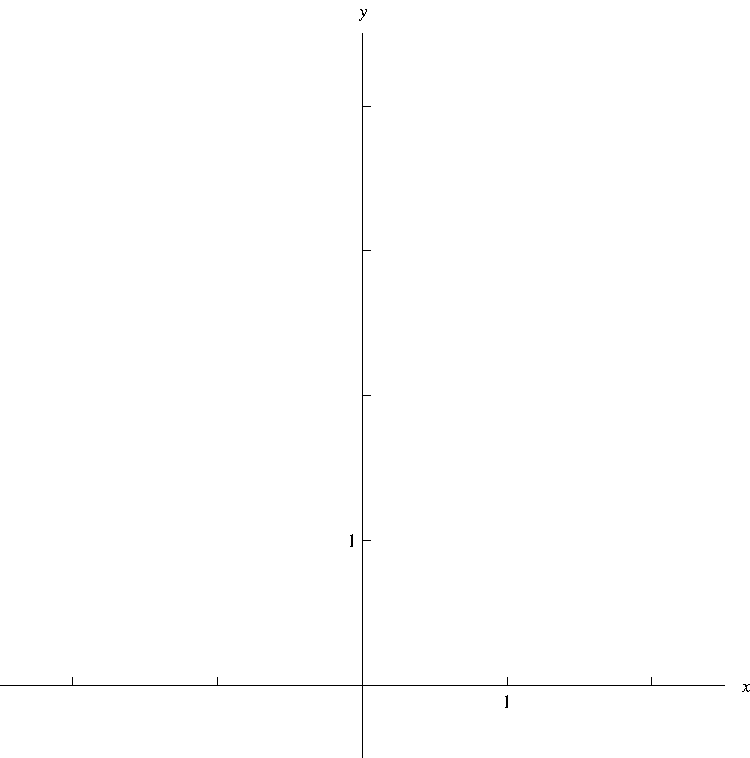
\includegraphics[height=6cm]{exponential-functions/pictures/twoxa.pdf}%
}%
\only<handout:0| 3-4>{%
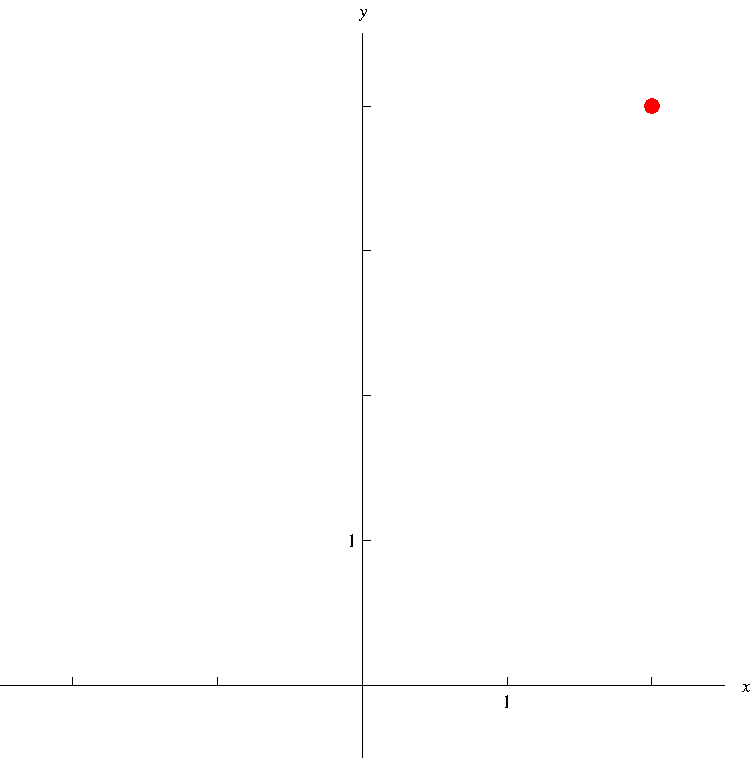
\includegraphics[height=6cm]{exponential-functions/pictures/twoxb.pdf}%
}%
\only<handout:0| 5-6>{%
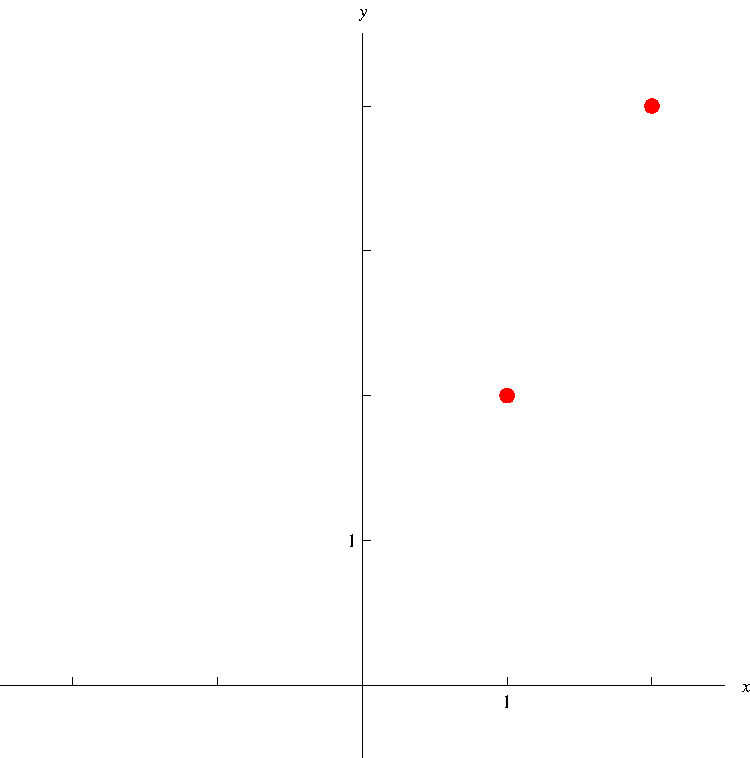
\includegraphics[height=6cm]{exponential-functions/pictures/twoxc.pdf}%
}%
\only<handout:0| 7-8>{%
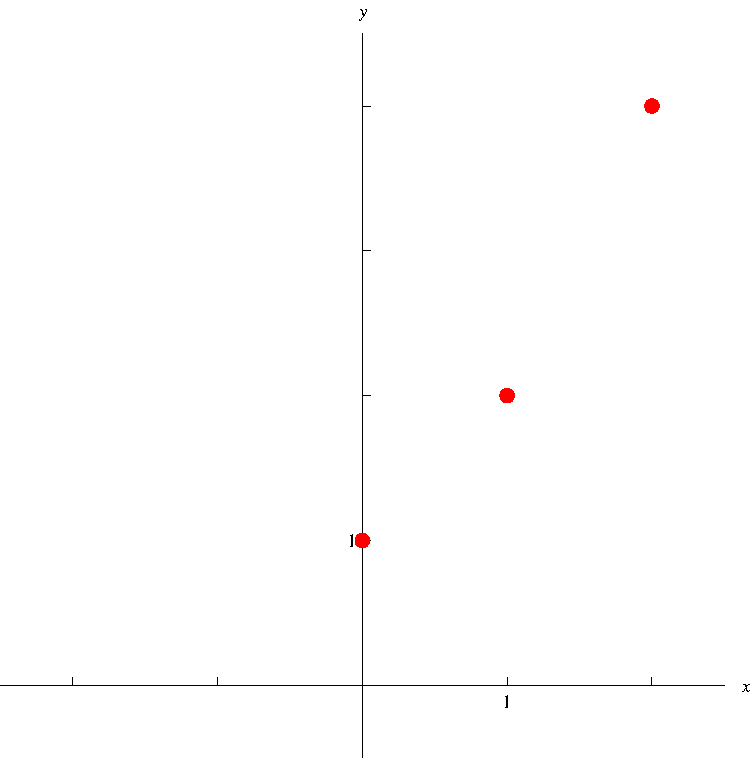
\includegraphics[height=6cm]{exponential-functions/pictures/twoxd.pdf}%
}%
\only<handout:0| 9-10>{%
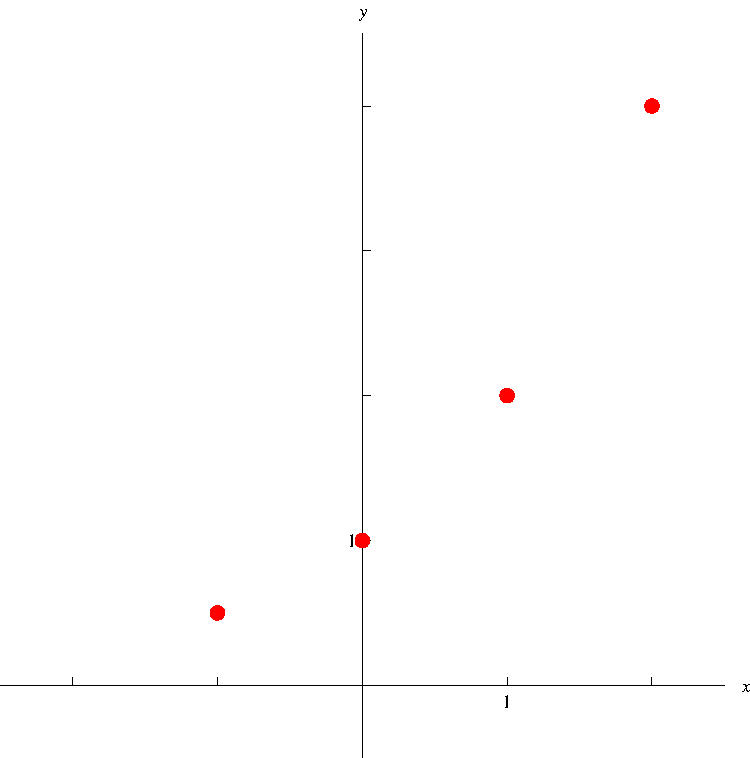
\includegraphics[height=6cm]{exponential-functions/pictures/twoxe.pdf}%
}%
\only<handout:0| 11>{%
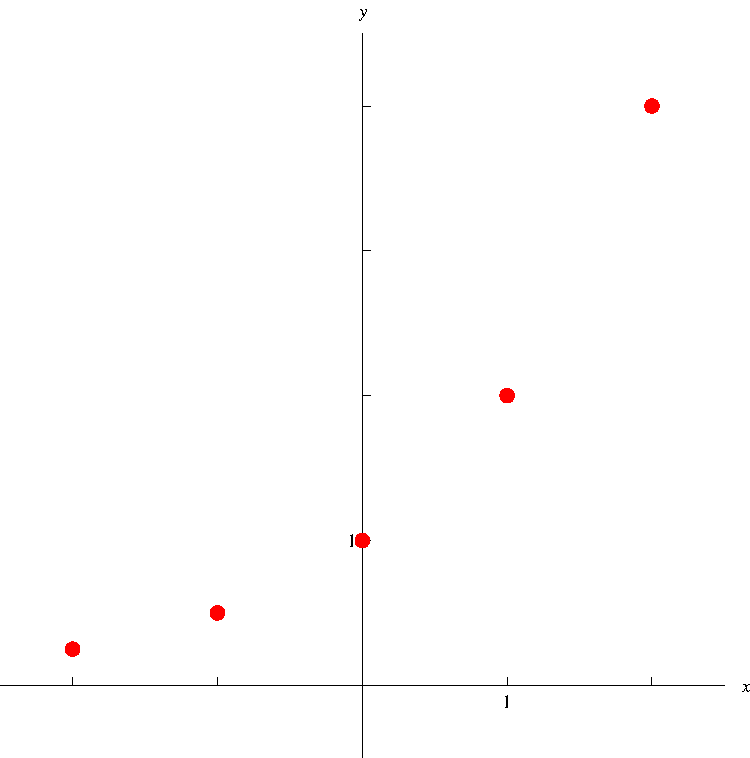
\includegraphics[height=6cm]{exponential-functions/pictures/twoxf.pdf}%
}%
\only<handout:1| 12->{%
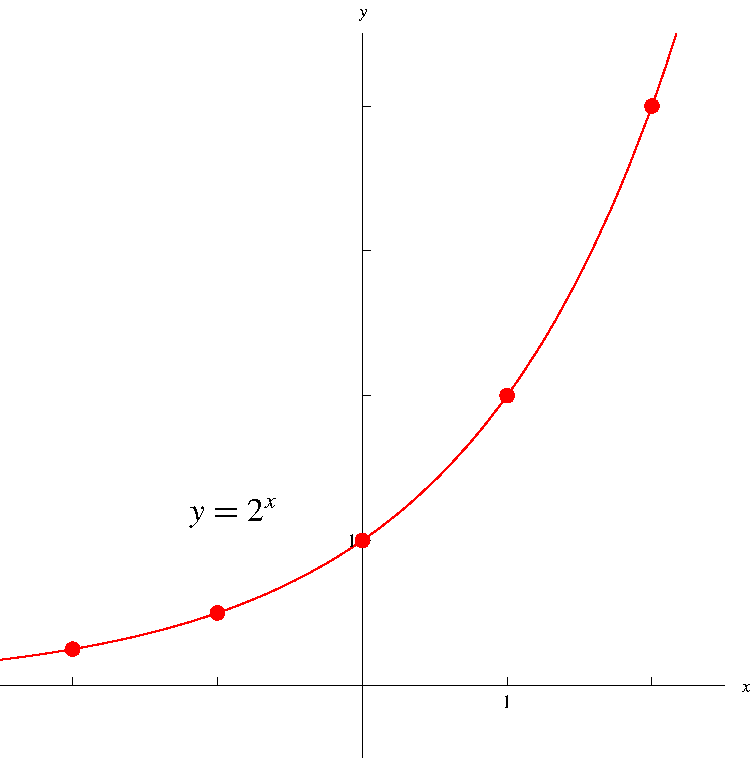
\includegraphics[height=6cm]{exponential-functions/pictures/twoxg.pdf}%
}%
\column{.5\textwidth}
\[
\begin{array}{r|l}
x & y\\
\hline
\alert<handout:0| 2-3>{2} & \alert<handout:0| 3>{\uncover<3->{4}} \\
\alert<handout:0| 4-5>{1} & \alert<handout:0| 5>{\uncover<5->{2}} \\
\alert<handout:0| 6-7>{0} & \alert<handout:0| 7>{\uncover<7->{1}} \\
\alert<handout:0| 8-9>{-1} & \alert<handout:0| 9>{\uncover<9->{1/2}} \\
\alert<handout:0| 10-11>{-2} & \alert<handout:0| 11>{\uncover<11->{1/4}} 
\end{array}
\]
\uncover<13->{
\begin{definition}[Exponential Function]
In general, an exponential function is a function of the form $f(x) = a^x$, where $a$ is a positive constant.
\end{definition}
}
\end{columns}
\end{frame}
% end module exponential-function-def

% begin module exponential-def-various-approaches
\begin{frame}
\frametitle{Exponents overview}
\begin{itemize}
\item<1-> Previously, for fixed $x$, we studied $a^{x}$ as a function of $a$. 
\item<2-> In present lecture we study $f(x)=a^x$ as a function of $x$.
\item<3-> A construction of $a^x$ was previously promised.
\item<4-> There are several equivalent ways of defining $a^x$. 
\item<5-> We give the easiest definition. 
\item<6-> We give a second equivalent definition. The second definition is studied in detail in Calculus II. 
\item<7->We discuss pros and cons.
\end{itemize}
\end{frame}
\begin{frame}
\frametitle{Exponent definition using limits (approach I)}
\begin{itemize}
\item<1-> For integer $p$ we know to compute $a^p$.
\item<2-> Therefore for integer $q$ we know to compute $a^{\frac{1}{q}}= \sqrt[q]{a}=\max\{x|\text{~for~which~} x^q\leq a\}$.
\item<3-> Therefore we know to compute $a^{\frac{p}{q}}$ for all rational $\frac{p}{q}$.
\item<4-> We can then define
\[
a^x = \lim\limits_{\substack{y \to x \\ y\text{-rational}}} a^y 
\]
\item<5-> Not computationally effective. It is not how computers compute.
\item<6-> However is the easiest approach. $a^{x+y}=a^xa^y$ is easiest to prove (follows directly from the $\varepsilon, \delta$-definition of $\lim$).
\item<7->\alert<7->{This is the definition assumed in Calculus I.}
\end{itemize}
\end{frame}
\begin{frame}
\frametitle{Exponent definition using series (approach II)}
\begin{itemize}
\item<1-> The Calc II formula can be used as alternative definition.
\[
e^{x}=\alert<4>{\sum_{n=0}^{\infty}} \frac{x^n}{\alert<2>{n!}}= 1+ x+\frac{x^2}{2!}+\frac{x^3}{3!}+\dots + \frac{x^{n}}{\alert<2>{n!}}+\dots
\]
\uncover<2->{\alert<2>{Here $n!=1\cdot 2\cdot 3\cdot\dots \cdot(n-1)\cdot n$ and is read ``$n$ factorial''. }}
\item<3-> For $|x|<1$ define 
\[
\ln (1+x)=\alert<4>{\sum_{n=1}^{\infty}} (-1)^{n+1}\frac{x^n}{n}=  x-\frac{x^2}{2}+\frac{x^3}{3}-\dots + \frac{(-1)^{n+1}x^{n}}{n}+\dots
\]
\uncover<4->{\alert<4>{Infinite sum studied in Calc II.}} 
\item<5-> For arbitrary $a>0$ define $a^x$ as $a^x=e^{x\ln a}$. 
\item<6-> Disadvantage: more difficult to prove $e^{x+y}=e^{x}e^y$ and $e^{\ln(1+x)}=1+x$, proof done in Calculus II.
\item<7-> This is how computers compute $e^x$ and $a^x$.
\end{itemize}
\end{frame}

% end module exponential-def-various-approaches

% begin module exponential-function-graphs
\begin{frame}
\begin{center}
Graphs of various exponential functions.

\psset{xunit=2cm, yunit=2cm}
\begin{pspicture}(-5, -5)(5,5) 
\psframe*[linecolor=white](-5,-5)(5,5) 
\psaxes[labels=none]{<->}(0,0)(-2.1,-0.2)(2.1,3.5)
\uncover<1->{
\rput[r](1.8, 2.3){$y=2^x$}
%Function formula: 2^{x} 
\psplot[linecolor=red, plotpoints=1000]{-2}{1.584962501}{2 x exp }
}
\uncover<2->{
\rput[l](1.2, 3.1){$y=4^x$}
%Function formula: 4^{x} 
\psplot[linecolor=black, plotpoints=1000]{-2}{0.79248125}{4 x exp }
}
\uncover<3->{
\rput[b](0.4, 3.05){$y=10^x$}
%Function formula: 4^{x} 
\psplot[linecolor=blue, plotpoints=1000]{-2}{0.477121255}{10 x exp }
}
\uncover<4->{
\rput[l](1.15, 1.5){$y=1.5^x$}
%Function formula: 4^{x} 
\psplot[linecolor=green, plotpoints=1000]{-2}{2}{1.5 x exp }
}
\uncover<5->{
\rput[l](-1.9, 2){$y=0.5^x$}
%Function formula: 4^{x} 
\psplot[linecolor=purple, plotpoints=1000]{-1.584962501}{2}{0.5 x exp }
}
\uncover<6->{
\rput[l](-1.2, 3.1){$y=0.25^x$}
%Function formula: 4^{x} 
\psplot[linecolor=brown, plotpoints=1000]{-0.79248125}{2}{0.25 x exp }
}
\end{pspicture}
\pause\pause\pause\pause\pause
%\ \only<handout:0| -1>{%
%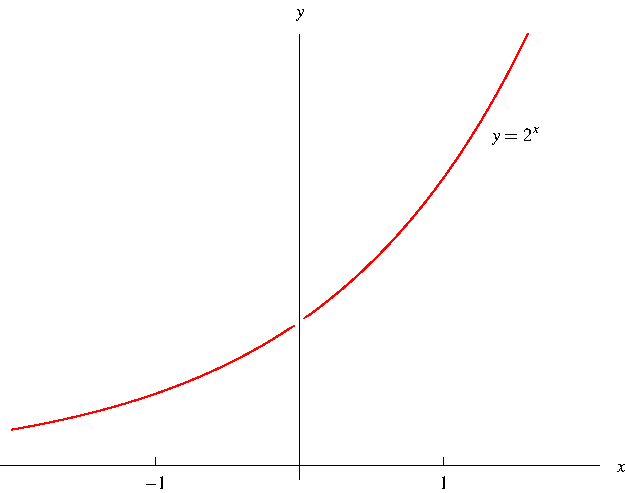
\includegraphics[height=6cm]{exponential-functions/pictures/07-02-manyexpa.pdf}%
%}%
%\only<handout:0| 2>{%
%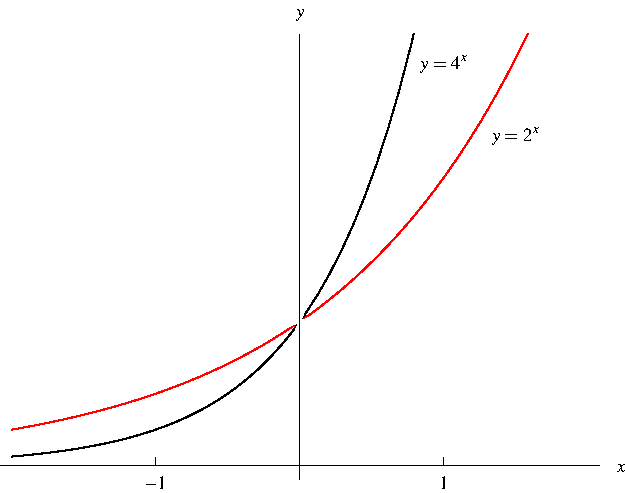
\includegraphics[height=6cm]{exponential-functions/pictures/07-02-manyexpb.pdf}%
%}%
%\only<handout:0| 3>{%
%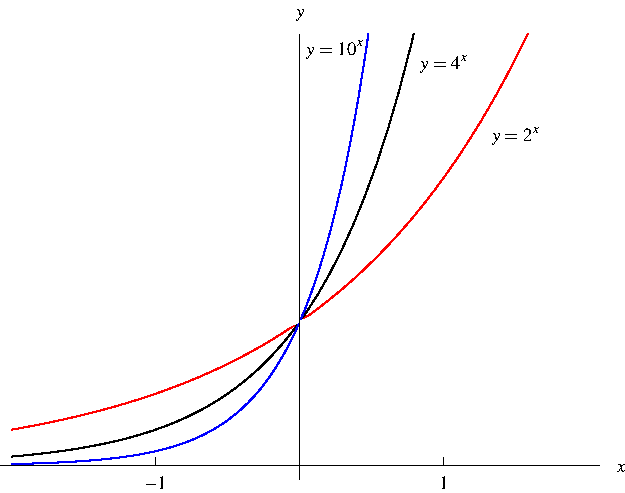
\includegraphics[height=6cm]{exponential-functions/pictures/07-02-manyexpc.pdf}%
%}%
%\only<handout:0| 4>{%
%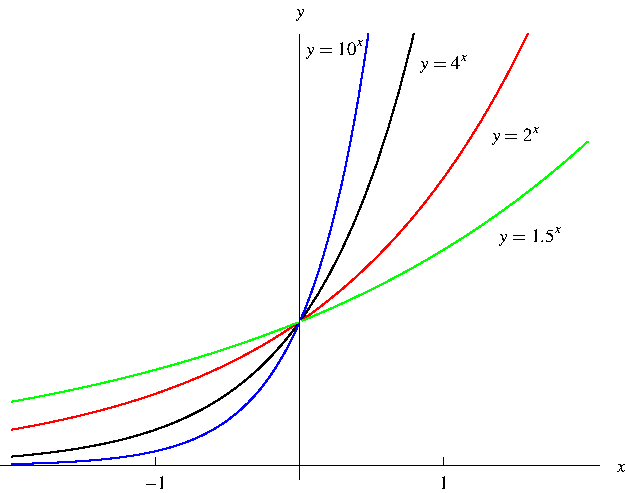
\includegraphics[height=6cm]{exponential-functions/pictures/07-02-manyexpd.pdf}%
%}%
%\only<handout:0| 5>{%
%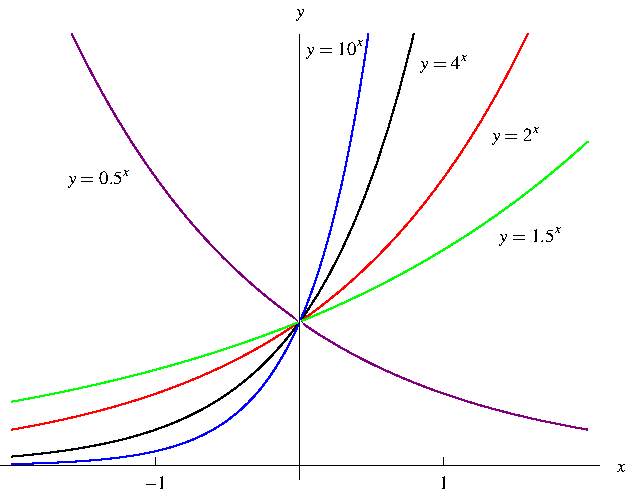
\includegraphics[height=6cm]{exponential-functions/pictures/07-02-manyexpe.pdf}%
%}%
%\only<6->{%
%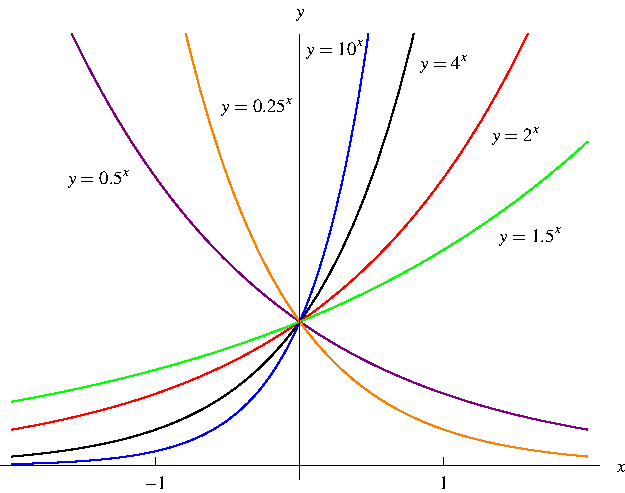
\includegraphics[height=6cm]{exponential-functions/pictures/07-02-manyexpf.pdf}%
%}%

\end{center}
\end{frame}
% end module exponential-function-graphs

% begin module exponential-versus-polynomial
\begin{frame}
\begin{center}
\small
Graphical comparison of $y = 2^x$ with $y = x^2$. Axes have different scales.
\begin{tabular}{cc}
\uncover<1->{
\psset{xunit=0.8cm, yunit=0.1cm}
\begin{pspicture}(-5, -5)(5,5) 
\psframe*[linecolor=white](-5,-5)(5,5) 
\psaxes[ticks=x, labels=x]{<->}(0,0)(-1,-3)(5.01,60)
\psline(-0.1,40)(0.1, 40)
\rput[l](0.2, 40){$40$} 
\psline(-0.1,20)(0.1, 20)
\rput[l](0.2, 20){$20$} 
%Function formula: 2^{x} 
\psplot[linecolor=red, plotpoints=1000]{-0.5}{5}{2 x exp }
\psplot[linecolor=blue, plotpoints=1000]{-0.5}{5}{x 2 exp }
\end{pspicture}
%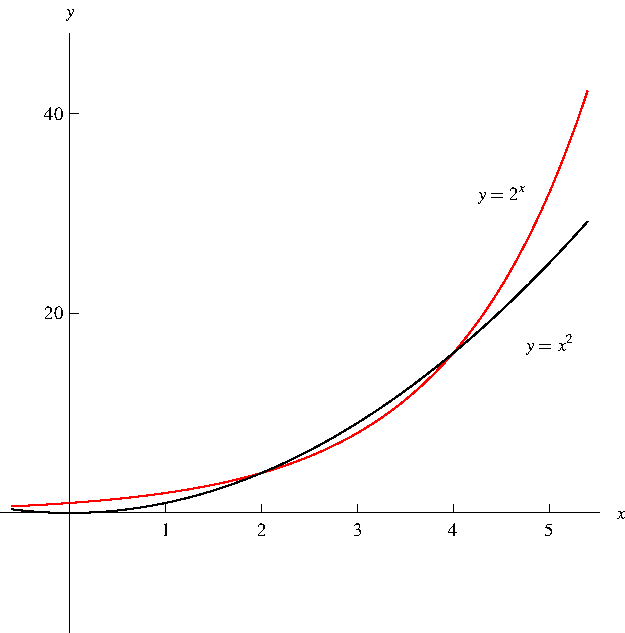
\includegraphics[height=5cm]{exponential-functions/pictures/07-02-expvspowera.pdf}%
}
&%
\uncover<2->{
\psset{xunit=0.25cm, yunit=0.05cm}
\begin{pspicture}(-5, -5)(5,5) 
\psframe*[linecolor=white](-5,-5)(5,5) 
\psaxes[ticks=x, Dx=4, labels=x]{<->}(0,0)(-1,-8)(16,120)
\psline(-0.4,100)(0.4, 100)
\rput[l](0.6, 100){$100$} 
%Function formula: 2^{x} 
\psplot[linecolor=red, plotpoints=1000]{-0.5}{7}{2 x exp }
\psplot[linecolor=blue, plotpoints=1000]{-0.5}{11.313708499}{x 2 exp }
\psline(-0.5, -3.5)(5, -3.5)(5, 32)(-0.5, 32)(-0.5, -3.5)
\rput[l](6, 10){Magnified region}
\end{pspicture}
%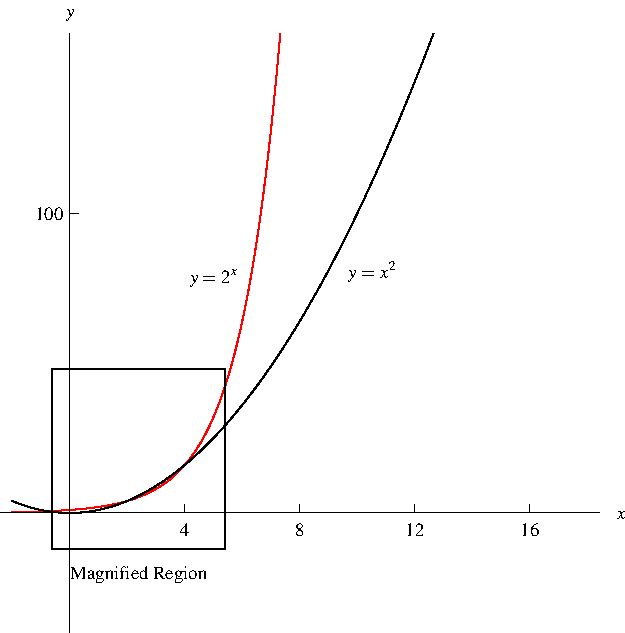
\includegraphics[height=5cm]{exponential-functions/pictures/07-02-expvspowerb.pdf}%
}
\end{tabular}
\end{center}
\end{frame}
% end module exponential-versus-polynomial
% begin module exponential-function-ex-sketch
\begin{frame}
\begin{example}
Draw the graph of the function $y = 2^{-x}-1$.
\only<handout:0| -1>{%
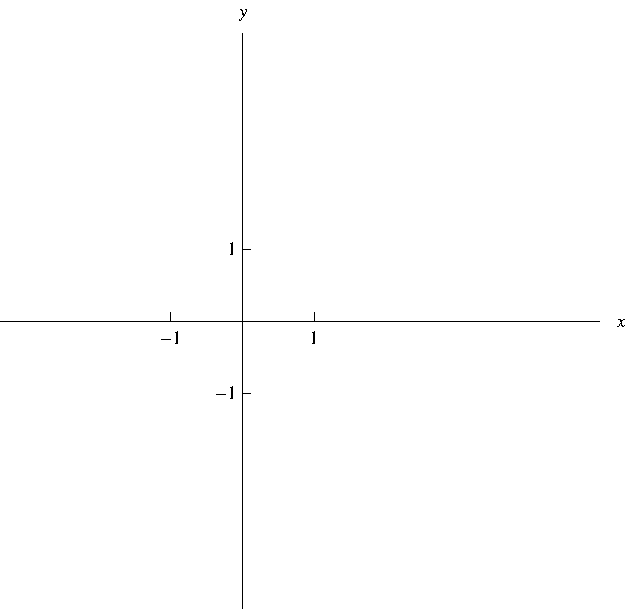
\includegraphics[height=7cm]{exponential-functions/pictures/07-02-ex1a.pdf}%
}%
\only<handout:0| 2>{%
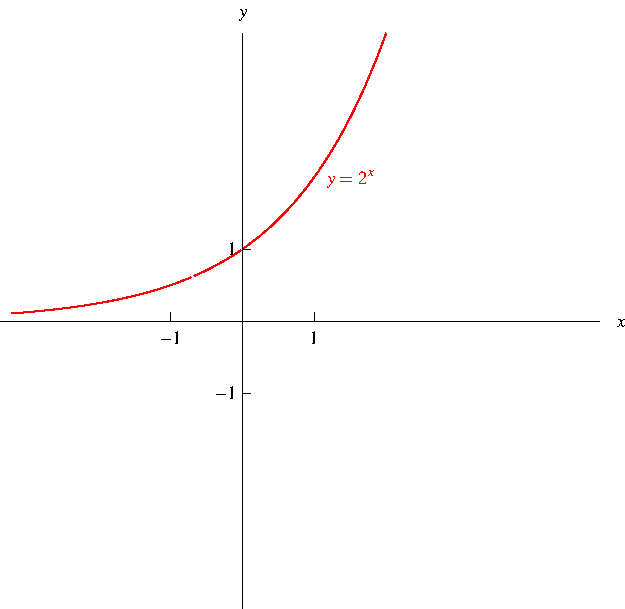
\includegraphics[height=7cm]{exponential-functions/pictures/07-02-ex1b.pdf}%
}%
\only<handout:0| 3>{%
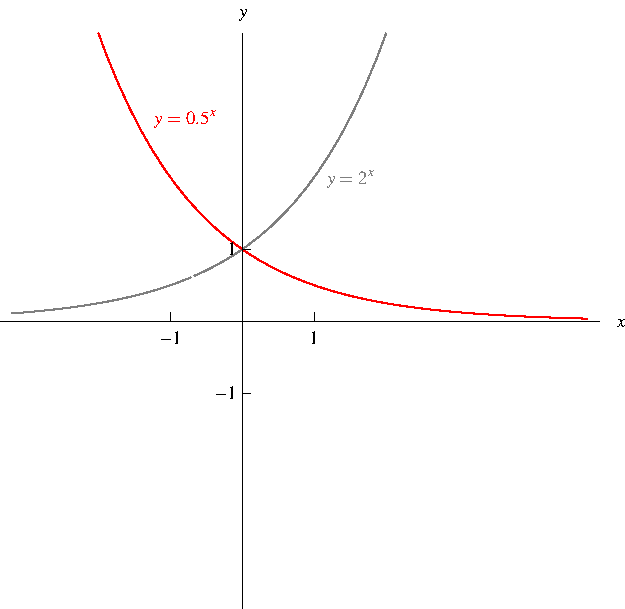
\includegraphics[height=7cm]{exponential-functions/pictures/07-02-ex1c.pdf}%
}%
\only<4->{%
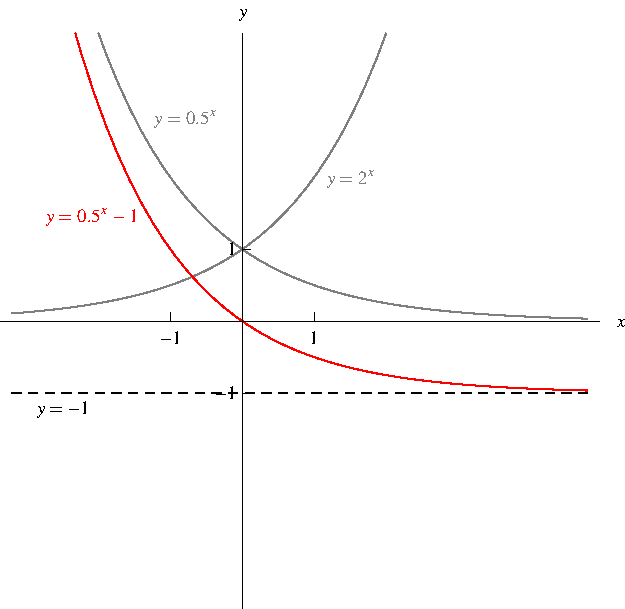
\includegraphics[height=7cm]{exponential-functions/pictures/07-02-ex1d.pdf}%
}%
\end{example}
\end{frame}
% end module exponential-function-ex-sketch

\section{Derivatives of Exponential Functions}
% begin module exponential-function-derivative
\begin{frame}
\frametitle{Derivatives of Exponential Functions}
Compute the derivative of $f(x) = a^x$ using the definition:
\begin{eqnarray*}
\uncover<2->{f'(x) = \lim_{h\rightarrow 0} \frac{f(x+h)-f(x)}{h}} & \uncover<3->{=} & \uncover<3->{\lim_{h\rightarrow 0} \frac{a^{x+h}-a^x}{h}}\\
 & \uncover<4->{=} & \uncover<4->{\lim_{h\rightarrow 0} \frac{a^x a^h-a^x}{h}}\\
 & \uncover<5->{=} & \uncover<5->{\lim_{h\rightarrow 0} \frac{a^x (a^h- 1)}{h}}\\
 & \uncover<6->{=} & \uncover<6->{a^x \lim_{h\rightarrow 0} \frac{a^h- 1}{h}}\\
\end{eqnarray*}
\uncover<7->{%
Note that the limit is the value of the derivative at 0; that is,
\[
f'(0) = \lim_{h\rightarrow 0}\frac{a^h-1}{h} .
\]
}%
\end{frame}


\begin{frame}
We have shown that, if $f(x) = a^x$ is differentiable at 0, then it is differentiable everywhere, and
\[
f'(x) = f'(0)a^x .
\]
\uncover<2->{
It is a fact that, for all positive $a$, the limit $\lim_{h\rightarrow 0}\frac{a^h - 1}{h}$ exists (we will not prove this).  Approximations for $a = 2$ and $a = 3$ appear below.
\[
\lim_{h\rightarrow 0}\frac{2^h - 1}{h} \approx 0.693147, \qquad %
\lim_{h\rightarrow 0}\frac{3^h - 1}{h} \approx 1.098612.
\]
}
\uncover<3->{
Then the derivative of $f(x) = a^x$ exists for all positive $a$.  Approximations for $a = 2$ and $a = 3$ appear below.
\[
\frac{\diff }{\diff x}(2^x) \approx (0.69)2^x, \qquad %
\frac{\diff }{\diff x}(3^x) \approx (1.10)3^x.
\]
}
\end{frame}
% end module exponential-function-derivative

\subsection{The Natural Exponential Function}
% begin module natural-exponential-intro
\begin{frame}
\frametitle{The Natural Exponential Function}
\begin{itemize}
\item  One base for an exponential function is especially useful.
\item<2->  It has a special property: its tangent line at $x = 0$ has slope $m=1$.
\item<3->  We call this number $e$, known as Euler's number or Napier's constant.
\item<4->  $e$ is a number between 2 and 3.  
\item<5-> In fact, $e = 1+1+\frac{1}{2!}+\frac{1}{3!} +\frac{1}{4!}+\dots\approx 2.71828$.  
\end{itemize}

\begin{columns}
\column{.3\textwidth}
\psset{xunit=1.3cm, yunit=1.3cm}
\begin{pspicture}(-1.4, -0.5)(1.4,2.6)
\psaxes[labels=none]{<->}(0,0)(-1.3, -0.5)(1.3,2.5)
\psplot[linecolor=red, plotpoints=1000]{-1.3}{1.3}{2 x exp}
\rput[r](-0.2, 1.1){\footnotesize $y=2^x$}
\rput[l](0.2, 0.8){\tiny $m\approx 0.693147$} 
\psline[linecolor=blue](-1.3,0.098908665)(1.3, 1.901091335)
\end{pspicture}
%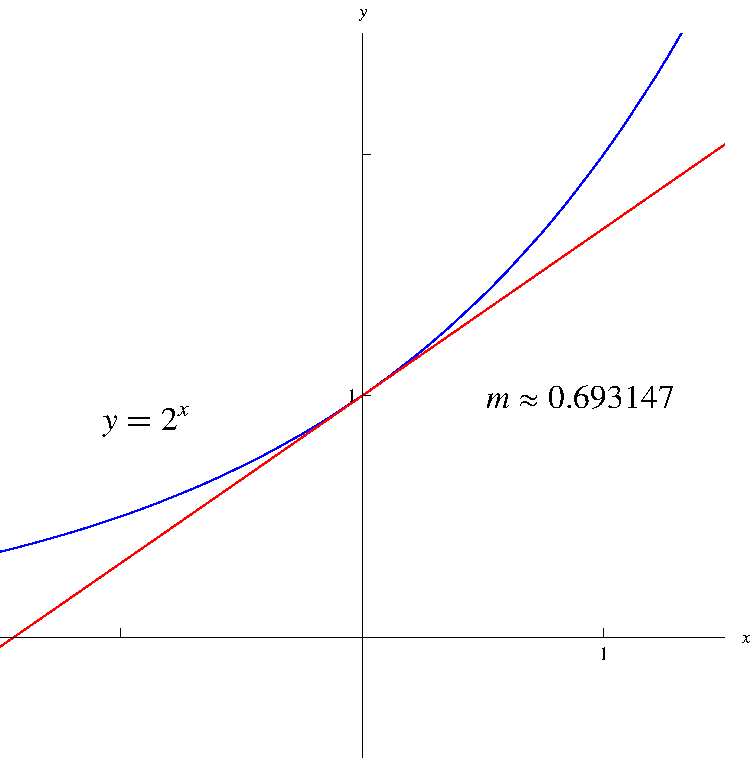
\includegraphics[height=4cm]{exponential-functions/pictures/exp-tangent-two.pdf}%
\column{.3\textwidth}
\uncover<handout: 1|3->{%
\psset{xunit=1.3cm, yunit=1.3cm}
\begin{pspicture}(-1.4, -0.5)(1.4,2.6)
\psaxes[labels=none]{<->}(0,0)(-1.3, -0.5)(1.3,2.5)
\psplot[linecolor=red, plotpoints=1000]{-1.3}{0.901091335}{2.718281828 x exp}
\rput[r](-0.2, 1.1){\footnotesize $y=e^x$}
\rput[l](0.2, 0.8){\tiny $m=1$}
\psline[linecolor=blue](-1.3, -0.3)(1.3,2.3) 
\end{pspicture}
%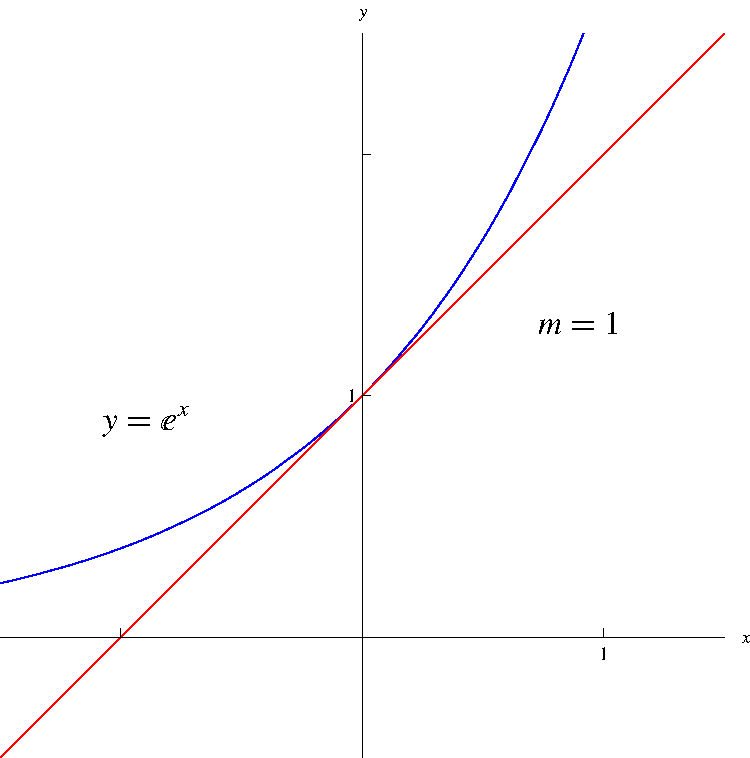
\includegraphics[height=4cm]{exponential-functions/pictures/exp-tangent-e.pdf}%
}%
\column{.3\textwidth}
\psset{xunit=1.3cm, yunit=1.3cm}
\begin{pspicture}(-1.4, -0.5)(1.4,2.6)
\psaxes[labels=none]{<->}(0,0)(-1.3, -0.5)(1.3,2.5)
\psplot[linecolor=red, plotpoints=1000]{-1.3}{0.82020868}{3 x exp}
\rput[r](-0.2, 1.1){\footnotesize $y=3^x$}
\rput[l](0.2, 0.8){\tiny $m\approx 1.09861$} 
\psline[linecolor=blue](-1.3, -0.428195975)(1.3,2.428195975)
\end{pspicture}
%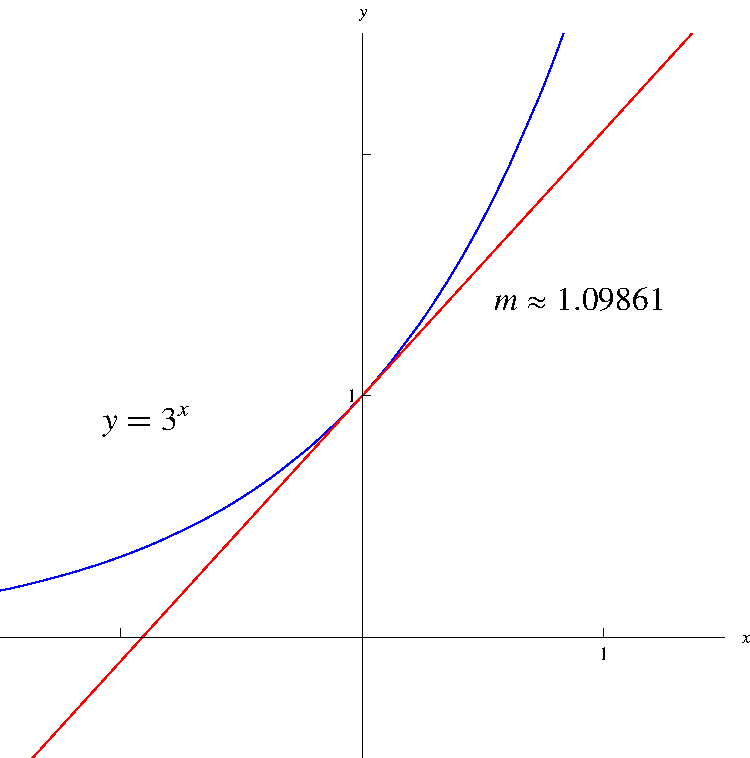
\includegraphics[height=4cm]{exponential-functions/pictures/exp-tangent-three.pdf}%
\end{columns}
\end{frame}
% end module natural-exponential-intro
% begin module e-def
\begin{frame}
\[
\text{If}\quad  f(x) = a^x, \quad \text{then}\quad f'(x) = f'(0)a^x .
\]
The formula above is simplest when $f'(0) = 1$.  Since $\lim\limits_{h\rightarrow 0}\frac{2^h-1}{h}\approx 0.69$ and $\lim\limits_{h\rightarrow 0}\frac{3^h-1}{h}\approx 1.10$, we expect there is a number $a$ between 2 and 3 such that $\lim\limits_{h\rightarrow 0}\frac{a^h-1}{h} = 1$.  
\uncover<2->{
\begin{definition}[$e$]
$e$ is the number such that $\lim\limits_{h\rightarrow 0}\frac{e^h-1}{h} = 1$.
\end{definition}
}

\begin{columns}
\column{.3\textwidth}
\psset{xunit=1.1cm, yunit=1.1cm}
\begin{pspicture}(-1.3, -0.5)(1.4,2.5) 
\psframe*[linecolor=white](-1.3,-0.5)(1.5,2.5) 
\psaxes[labels=none]{<->}(0,0)(-1.3, -0.5)(1.3,2.5)
\psplot[linecolor=red, plotpoints=1000]{-1.3}{1.3}{2 x exp}
\rput[r](-0.2, 1.1){\footnotesize $y=2^x$}
\rput[l](0.2, 0.8){\tiny $m\approx 0.693147$} 
\psline[linecolor=blue](-1.3,0.098908665)(1.3, 1.901091335)
\end{pspicture}
%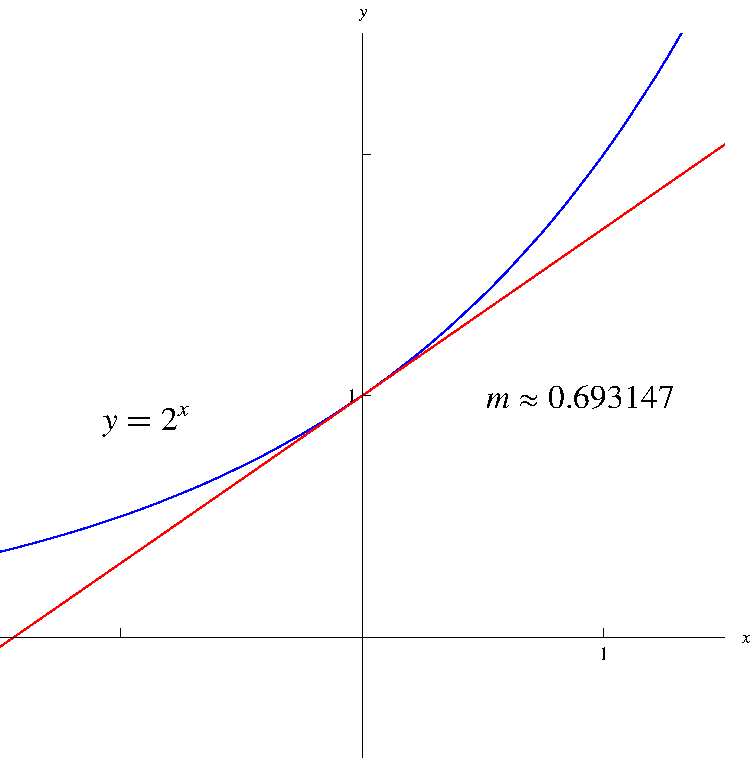
\includegraphics[height=4cm]{exponential-functions/pictures/exp-tangent-two.pdf}%
\column{.3\textwidth}
\uncover<handout: 1|3->{%
\psset{xunit=1.1cm, yunit=1.1cm}
\begin{pspicture}(-1.3, -0.5)(1.4,2.6) 
\psframe*[linecolor=white](-1.3,-0.5)(1.4,2.6) 
\psaxes[labels=none]{<->}(0,0)(-1.3, -0.5)(1.3,2.5)
\psplot[linecolor=red, plotpoints=1000] {-1.3}{0.901091335}{2.718281828 x exp}
\rput[r](-0.2, 1.1){\footnotesize $y=e^x$}
\rput[l](0.2, 0.8){\tiny $m=1$}
\psline[linecolor=blue](-1.3, -0.3)(1.3,2.3) 
\end{pspicture}
%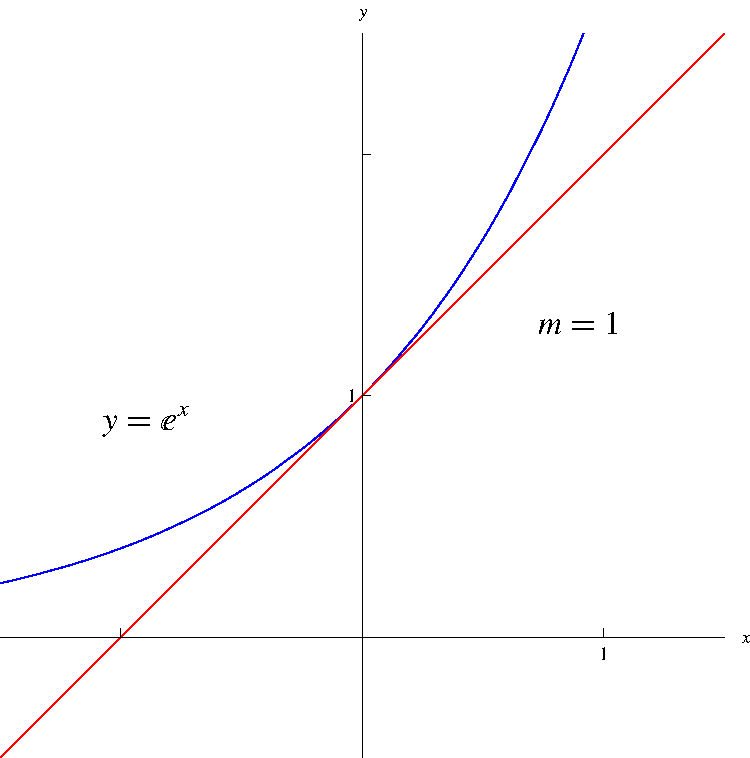
\includegraphics[height=4cm]{exponential-functions/pictures/exp-tangent-e.pdf}%
}%
\column{.3\textwidth}
\psset{xunit=1.1cm, yunit=1.1cm}
\begin{pspicture}(-1.3, -0.5)(1.4,2.6) 
\psframe*[linecolor=white](-1.3,-0.5)(1.4,2.6) 
\psaxes[labels=none]{<->}(0,0)(-1.3, -0.5)(1.3,2.5)
\psplot[linecolor=red, plotpoints=1000]{-1.3}{0.82020868}{3 x exp}
\rput[r](-0.2, 1.1){\footnotesize $y=3^x$}
\rput[l](0.2, 0.8){\tiny $m\approx 1.09861$} 
\psline[linecolor=blue](-1.3, -0.428195975)(1.3,2.428195975)
\end{pspicture}
%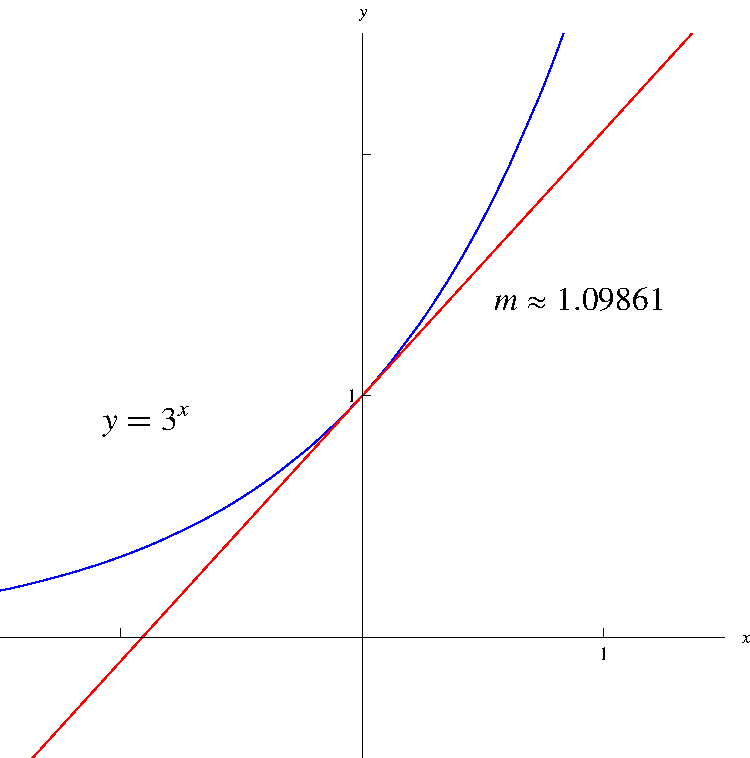
\includegraphics[height=4cm]{exponential-functions/pictures/exp-tangent-three.pdf}%
\end{columns}
\end{frame}
% end module e-def

% begin module natural-exponential-def
\begin{frame}
\begin{definition}[Natural Exponential Function]
$e^x$ is called the natural exponential function.  Its derivative is
\[
\frac{\diff}{\diff x} \left(e^x\right) = e^x .
\]
\end{definition}
\end{frame}
% end module natural-exponential-def

\subsection{Derivative using series definition}
% begin module power-rule-rationa-from-chain-rule
\begin{frame}

\begin{example}
Derive \alert<11>{the exponent rule $\left(e^x\right)'=e^x$} \uncover<2->{using the Calc II formula below,} \uncover<3->{ \alert<3>{the infinite} {\color{gray!50} (both sides uniformly convergent)} \alert<3>{sum rule $(f_1+f_2 +f_3 +\dots)' =f_1' +f_2'  +f_3' +\dots$}}
\uncover<4->{and \alert<4>{the power rule $(x^n)'=nx^{n-1}$}. } 
\uncover<2->{\[
\alert<2,10>{e^x}=\alert<2,10>{1+x+\frac{x^2}{2!}+\frac{x^3}{3!}+\dots},
\]
}
\uncover<2->{where $n!=1\cdot2\cdot3\cdot \dots\cdot n$.} \uncover<5->{We have that $\alert<5,9>{\frac{n}{\alert<6>{ n!}}} =\uncover<6->{ \frac{\alert<7>{n} }{ \alert<6>{ 1\cdot 2\cdot \dots\cdot (n-1) \cdot  \alert<7>{n}}}=}\uncover<7->{\frac{1}{\alert<8>{1\cdot 2\cdot \dots\cdot (n-1)}}=}\uncover<8->{\alert<9>{ \frac{1}{ \alert<8>{(n-1)!} }}} $.}
\[
\begin{array}{rcl}
\uncover<2->{\alert<11>{\left(\alert<2>{e^x}\right)'} &=&\alert<3>{\left(\alert<2>{1+x+\frac{x^2}{2!}+\frac{x^3}{3!}+\dots} \right)' }} \\
\uncover<3->{&=& \alert<3>{ \alert<4>{(1)'}+\alert<4>{(x)'}+\frac{\alert<4>{(x^2)'}}{2!} +\frac{\alert<4>{(x^3)'}}{3!}+\dots + \frac{\alert<4>{(x^n)'}}{n!}+\dots}}
\\ \uncover<4->{&=&\alert<4>{0}+ \alert<4>{1}+ \frac{\alert<4>{\alert<5-9>{2}x}}{\alert<5-9>{2!}}+ \frac{\alert<4>{\alert<5-9>{3}x^2}}{\alert<5-9>{3!}}+ \dots +\frac{\alert<4>{\alert<5-9>{n}x^{n-1}}}{\alert<5-9>{n!}}+\dots }\\
\uncover<9->{&=& \alert<10>{ \phantom{ 0~ + }  1 + \frac{\phantom{2}x}{\alert<9>{1!}}+\frac{\phantom{3}x^{2}}{\alert<9>{2!}}+\dots+\frac{\phantom{n}x^{n-1}}{\alert<9>{(n-1)!}}+\dots}=}\uncover<10->{\alert<10,11>{e^x}}\\
\end{array}
\]
\uncover<11->{\alert<11>{as desired.}}
\end{example}

\end{frame}

%end module power-rule-rationa-from-chain-rule
% begin module derivative-e-plus-polynomial
\begin{frame}
\begin{example}[Derivative of a Polynomial and the Natural Exponential Function]
\abovedisplayskip=0pt
\belowdisplayskip=-15pt
\abovedisplayshortskip=0pt
\belowdisplayshortskip=0pt
\begin{align*}
\text{Differentiate}\quad y & = e^x+x^7.\\
\uncover<2->{\frac{\diff y}{\diff x} & = \alertNoH{3-4}{\frac{\diff}{\diff x}(e^x)} + \alertNoH{5-6}{\frac{\diff}{\diff x}(x^7)}}\\
& \uncover<3->{= \fcAnswer{4}{\alertNoH{4}{e^x}}  + \fcAnswerUncover{3}{6}{\alertNoH{6}{7x^6}.}}
\end{align*}
\end{example}
\end{frame}
% end module derivative-e-plus-polynomial

}% end lecture

% begin lecture
\lect{January 27-31, 2014}{Lecture 2}{2}{
\section{Inverse Functions, Review}
\subsection{One-to-one Functions}
% begin module one-to-one-def
\begin{frame}
\frametitle{One-to-one Functions}
\begin{definition}[One-to-one Function]
A function $f$ is a one-to-one function if it never takes on the same value twice; that is,
\[
f(x_1) \neq f(x_2) \ \text{whenever }  \ x_1 \neq x_2 .
\]
\end{definition}
\begin{columns}[c]
\column{.5\textwidth}
\psset{xunit=1.3cm, yunit=1.3cm}
\begin{pspicture}(-5, -5)(5,5) 
\psframe*[linecolor=white](-5,-5)(5,5) 
\psaxes[ticks=none, labels=none]{<->}(0,0)(-0.5,-0.5)(3.9,3)
%Function formula: -1/2*((-17/10+x)^{2})+9/5 
\psplot[linecolor=red, plotpoints=1000]{-0.5}{3.9}{1.8 x -1.7 add 2 exp -0.5 mul add }
\rput[b](1.7, 1.9) {\footnotesize $y=f(x)$}

\psFullDot{0.7}{1.3}
\rput[br](0.6, 1.4) {\footnotesize $(x_1, f(x_1))$}
\psFullDot{2.7}{1.3}
\rput[bl](2.8, 1.4) {\footnotesize $(x_2, f(x_2))$}

\psline(-0.5, 1.3)(3, 1.3)
\rput[t](1.7, 1.2) {\footnotesize $y=f(x_1)=f(x_2)$}

\psline(0.7, -0.1)(0.7, 0.1)
\rput[t](0.7, -0.2){\footnotesize $x_1$}
\psline(2.7, -0.1)(2.7, 0.1)
\rput[t](2.7, -0.2){\footnotesize $x_2$}

\end{pspicture} 
%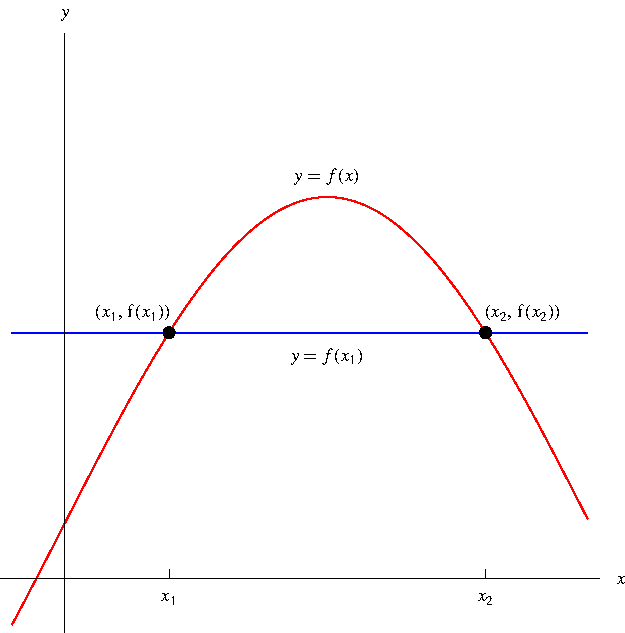
\includegraphics[height=5cm]{inverse-functions/pictures/07-01-1-1def.pdf}%
%
\column{.5\textwidth}
$\leftarrow$ This function is not one-to-one.
\end{columns}
\end{frame}
% end module one-to-one-def

% begin module horizontal-line-test
\begin{frame}
Question: How can we tell from the graph of a function whether it is one-to-one or not?

Answer: Use the horizontal line test.

\begin{proof}[The Horizontal Line Test]
A function is one-to-one if and only if no horizontal line intersects it more than once.
\end{proof}

\begin{tabular}{cc}
\psset{xunit=0.7cm, yunit=0.7cm}
\begin{pspicture}(-5, -5)(5,5) 
\psframe*[linecolor=white](-5,-5)(5,5) 
\psaxes[ticks=none, labels=none]{<->}(0,0)(-3,-3)(3,3)
%Function formula: 1/2 (x)+1/2 
\psplot[linecolor=red, plotpoints=1000]{1}{2}{0.5 x 0.5 mul add } %Function formula: (x)^{3} 
\psplot[linecolor=red, plotpoints=1000]{-1}{1}{x 3 exp } %Function formula: 3/2 (x)+1/2 
\psplot[linecolor=red, plotpoints=1000]{-2}{-1}{0.5 x 1.5 mul add }
\end{pspicture} 
%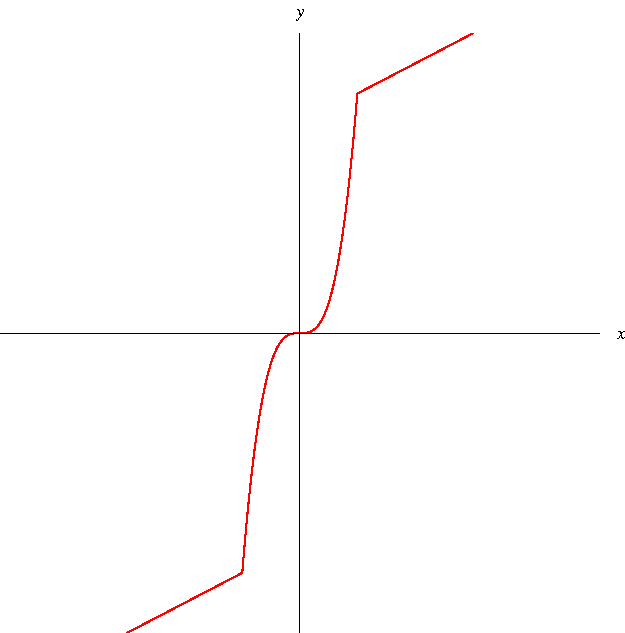
\includegraphics[height=4cm]{inverse-functions/pictures/07-01-onetoone.pdf} 
 %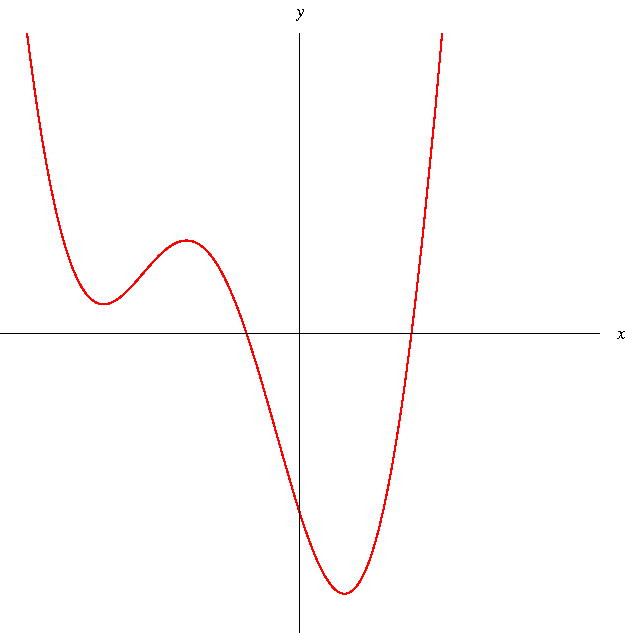
\includegraphics[height=4cm]{inverse-functions/pictures/07-01-notonetoonea.pdf}%
&%
\uncover<handout:0| 2->{%
\psset{xunit=0.7cm, yunit=0.7cm}
\begin{pspicture}(-5, -5)(5,5) 
\psframe*[linecolor=white](-5,-5)(5,5) 
\psaxes[ticks=none, labels=none]{<->}(0,0)(-3,-3)(3,3)
 %Function formula: -2/5+((6/5+x)^{2}) ((x) (x))-6/25 ((6/5+x)^{2})- (((6/5+x)^{2}) (x)) 
 \psplot[linecolor=red, plotpoints=1000]{-2}{1.5}{x x 1.2 add 2 exp mul -1 mul x 1.2 add 2 exp -0.24 mul add x x mul x 1.2 add 2 exp mul add -0.4 add }
 \uncover<3->{
 \psline[linestyle=dashed](-3, 1)(3, 1)
 }
 \end{pspicture} 
}
\\
\uncover<2->{\alert<handout:0| 2>{One-to-one}} &
\uncover<3->{\alert<handout:0| 3>{Not one-to-one}}
\end{tabular}
\end{frame}
% end module horizontal-line-test

\subsection{The Definition of the Inverse of $f$}
% begin module inverse-function-def
\begin{frame}
\frametitle{The Definition of the Inverse of $f$}
\begin{definition}[$f^{-1}$]
Let $f$ be a one-to-one function with domain $A$ and range $B$.  Then the inverse of $f$ is the function $f^{-1}$ that has domain $B$ and range $A$ and is defined by
\[
f^{-1}(y) = x \qquad \Leftrightarrow \qquad f(x) = y 
\]
for all $y$ in $B$.
\end{definition}
\begin{columns}[T]
\column{.5\textwidth}
\uncover<2->{Note:}
\begin{itemize}
\item<3->  Only one-to-one functions have inverses.
\item<4->  $f^{-1}$ reverses the effect of $f$.
\item<5->  domain of $f^{-1} = $ range of $f$.
\item<5->  range of $f^{-1} = $ domain of $f$.
\end{itemize}
\column{.5\textwidth}
\uncover<6->{
\begin{example}[$f(x) = x^3$]
The inverse of $f(x) = x^3$ is $f^{-1}(x) = \sqrt[3]{x}$.  This is because if $y = x^3$, then
\[
f^{-1}(y) = \sqrt[3]{y} = \sqrt[3]{x^3} = x .
\]
\end{example}
}
\end{columns}
\end{frame}
% end module inverse-function-def

% begin module inverse-notation-warning
\begin{frame}
\uncover<1->{The inverse of $f$ is denoted as $f^{-1}$.} \uncover<2->{This notation is one of the most frequent causes of student confusion.} \uncover<3->{\alert<3>{\textbf{WARNING:}}}
\uncover<3->{
\[
f^{\alert<4>{-1}} \alert<4>{(x)}  \text{ does not mean } \left(f \alert<5>{(x)}\right)^{\alert<5>{-1}} = \frac{1}{f(x)}\quad .
\]
}
\uncover<4->{The notations are  \alert<4,5>{different:} the superscript $-1$ has \alert<4,5>{different positions}.}
\begin{itemize}
\item<6->  $f^{-1}$ is the compositional inverse of $f$.
\item<7->  $\frac{1}{f(x)}$ is the multiplicative inverse of $f(x)$.
\item<8->  $f^{2}(x)$ is an abbreviation for $(f(x))^2$,  $f^{3}(x)$ is an abbreviation of $(f(x))^3$, and so on.
\item<9->  \alert<10>{\alert<9>{However, } $f^{-1}(x)$ is not the abbreviation of $\left(f(x)\right)^{-1}$ and does not follow this pattern.}
\end{itemize}

\only<10>{ \begin{quotation}
No one blamed English language of being logical.
\end{quotation}
-Bjarne Stroustrup, creator of the programming language C++
}

\uncover<11->{
\[
f^{n}(x)= \left\{ \begin{array}{ll} \alert<11>{\text{stands for } \left(f(x)\right)^n} & \alert<11>{ \text{when } n=1,2,3,\dots} \\
\alert<12>{\text{stands for inverse of } f \text{ applied to }x} & \alert<12>{ \text{when } n=-1} \\
\alert<13>{\text{should be avoided } } & \alert<13>{ \text{when } n\neq -1, 1,2,3,\dots .}
\end{array} \right.
\]
}
\uncover<14->{ To reduce confusion, if possible, use $\frac{1}{f(x)}$ instead of $\left(f(x)\right)^{-1}$.}


\vspace{8cm}
\end{frame}
% end module inverse-notation-warning

% begin module inverse-function-equations
\begin{frame}
\[
\alert<handout:0| 4>{f^{-1}(y) = x} \qquad \Leftrightarrow \qquad \alert<handout:0| 3>{f(x) = y} .
\]
\uncover<2->{Therefore
\[
(f^{-1}\circ f)(x) = f^{-1}(\alert<handout:0| 3>{f(x)}) = \uncover<3->{\alert<handout:0| 4>{f^{-1}(\alert<handout:0| 3-4>{y})}} \uncover<4->{\alert<handout:0| 4>{ = x}.}
\]
}
\uncover<5->{
\psset{xunit=0.75cm, yunit=0.75cm}
\begin{pspicture}(-4, -2)(13,2)
\footnotesize
\rput[r] (-3.1, 0){$x$}
\psline[linewidth=3pt]{->}(-3,0)(-2.25,0)

\rput(0.25,0){
\fcMachine{$f$}{red}
}
\rput (4, 0){$f(x)$}
\psline[linewidth=3pt]{->}(2.75,0)(3.5,0)
\psline[linewidth=3pt]{->}(4.5,0)(5.25,0)
\rput(7.75,0){
\fcMachine{$f^{-1}$}{blue}
}
\rput[l](11.25, 0){$x$}
\psline[linewidth=3pt]{->}(10.25,0)(11,0)
\end{pspicture}
%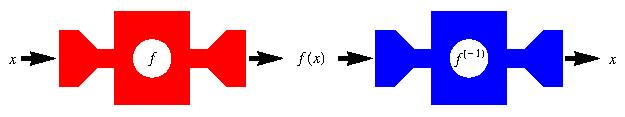
\includegraphics[height=2cm]{inverse-functions/pictures/07-01-machinesb.pdf}%
}
\uncover<6->{
Switch the roles of $x$ and $y$:
\[
\alert<handout:0| 8>{f^{-1}(x) = y} \qquad \Leftrightarrow \qquad \alert<handout:0| 9>{f(y) = x} .
\]
}
\uncover<7->{Therefore
\[
(f\circ f^{-1})(x) = f(\alert<handout:0| 8>{f^{-1}(x)}) = \uncover<8->{\alert<handout:0| 9>{f(\alert<handout:0| 8-9>{y})}} \uncover<9->{\alert<handout:0| 9>{ = x}.}
\]
}
\uncover<10->{
\psset{xunit=0.75cm, yunit=0.75cm}
\begin{pspicture}(-4, -2.5)(13,2.5)
\footnotesize
\rput[r] (-3.1, 0){$x$}
\psline[linewidth=3pt]{->}(-3,0)(-2.25,0)

\rput(0.25,0){
\fcMachine{$f^{-1}$}{blue}
}
\rput (4, 0){ $f^{-1}(x)$}
\psline[linewidth=3pt]{->}(2.75,0)(3.4,0)
\psline[linewidth=3pt]{->}(4.7,0)(5.25,0)
\rput(7.75,0){
\fcMachine{$f$}{red}
}
\rput (11.75, 0){$x$}
\psline[linewidth=3pt]{->}(10.25,0)(11,0)
\end{pspicture}
%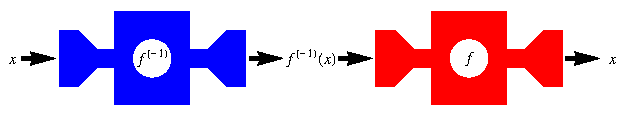
\includegraphics[height=2cm]{inverse-functions/pictures/07-01-machinesa.pdf}%
}
\end{frame}
% end module inverse-function-equations

% begin module inverse-function-solve-for
\begin{frame}
\frametitle{How to Find the Inverse of a One-to-one Function}
\begin{enumerate}
\item<1-| alert@3>  Write $y = f(x)$.
\item<1-| alert@4-5>  Solve this equation for $x$ in terms of $y$ (if possible).
\end{enumerate}
\uncover<2->{
\begin{example}%[Example 4, p. 388]
If $f(x) = x^3 + 2$, find a formula for $f^{-1}(y)$.
\begin{align*}
\uncover<3->{y} & \uncover<3->{=}  \uncover<3->{x^3 + 2}\\
\uncover<4->{x^3} & \uncover<4->{=}  \uncover<4->{y - 2}\\
\uncover<5->{\alert<handout:0| 6>{x}} & \uncover<5->{=}  \uncover<5->{\alert<6>{\sqrt[3]{y - 2}}}
\end{align*}
\uncover<6->{
Therefore \alert<6,8>{$x=f^{-1}(y) = \sqrt[3]{y - 2}$}.
}
\uncover<7->{
Sometimes we relabel $x$ and $y$ and write \only<7>{ $f^{-1}(x)=\sqrt[3]{x-2}$.} \only<8->{\color{gray!50} $f^{-1}(x)=\sqrt[3]{x-2}$.}
}
\uncover<8->{\alert<8>{
Whenever in doubt, do not relabel anything.
}}
\end{example}
}
\end{frame}
% end module inverse-function-solve-for

% begin module guess-and-check
\begin{frame}
\begin{example}[Guess and Check]
If $f(x) = 2x + \sin 2x + e^{x/2}$, find $f^{-1}(1)$.  
\begin{align*}
\uncover<2->{f\alert<handout:0| 2-3>{(\uncover<3-| handout:0>{0})}} & \uncover<2->{=}  \uncover<2->{2\alert<handout:0| 2-3>{(\uncover<3-| handout:0>{0})}  + \sin 2\alert<handout:0| 2-3>{(\uncover<3-| handout:0>{0})}  + e^{\alert<handout:0| 2-3>{(\uncover<3-| handout:0>{0})}/2} }\\ 
 & \uncover<2->{=}  \uncover<3-| handout:0>{0 + 0 + 1} \\
 & \uncover<2->{=}  \uncover<2->{1.} \\
\uncover<4->{\text{Therefore}\quad f^{-1}(1)} & \uncover<4->{=}  \uncover<4-| handout:0>{0.}
\end{align*}
\end{example}
\end{frame}
% end module guess-and-check

% begin module inverse-function-graph
\begin{frame}
\begin{tabular}{cc}
\psset{xunit=0.9cm, yunit=0.9cm}
\begin{pspicture}(-1.5,-1.5)(3.5,3.2)
\psaxes[ticks=none, labels=none]{<->}(0,0)(-1.5,-1.5)(3.4,3.1)
\fcLabels{3.4}{3.1}
\uncover<6->{
\psline(2.5, 1)(1, 2.5)
\psline(1.85, 1.65)(1.95, 1.75)(1.85, 1.85)
\psline(1.85, 1.85)(1.75, 1.95)(1.65, 1.85)

\psline(1.9875, 1.3125)(2.1875, 1.5125)
\psline(2.0625, 1.2375)(2.2625, 1.4375)
\psline(1.3125, 1.9875)(1.5125, 2.1875)
\psline(1.2375, 2.0625)(1.4375, 2.2625)

\psline[linecolor=blue](-1.35, -1.35)(2.8,2.8)
\rput[l](-1, -1.2){\footnotesize $y=x$}
}
\uncover<2->{
\fcFullDot{2.5}{1}
\rput[lt](2.6, 1.1){\footnotesize $(a,b)$}
}
\uncover<5->{
\fcFullDot{1}{2.5}
\rput[rb](0.9, 2.6){\footnotesize $(b,a)$}
}
\end{pspicture}
%\ \only<handout:0| -4>{%
%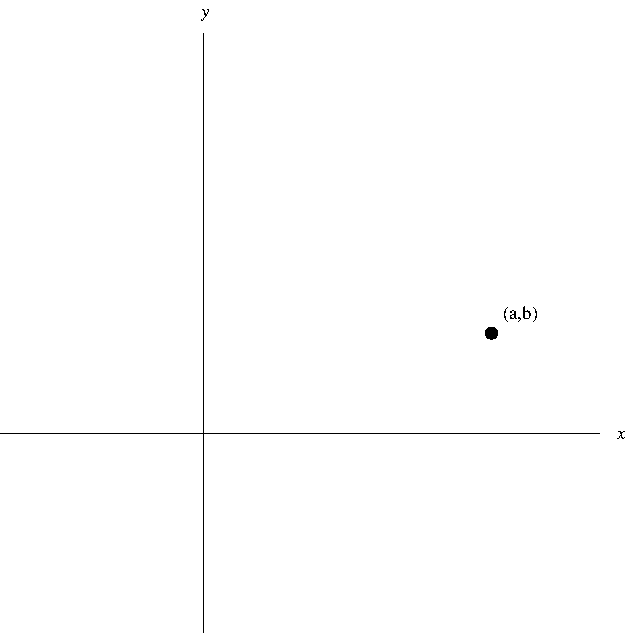
\includegraphics[height=4cm]{inverse-functions/pictures/07-01-reflecta.pdf}%
%}%
%\only<handout:0| 5>{%
%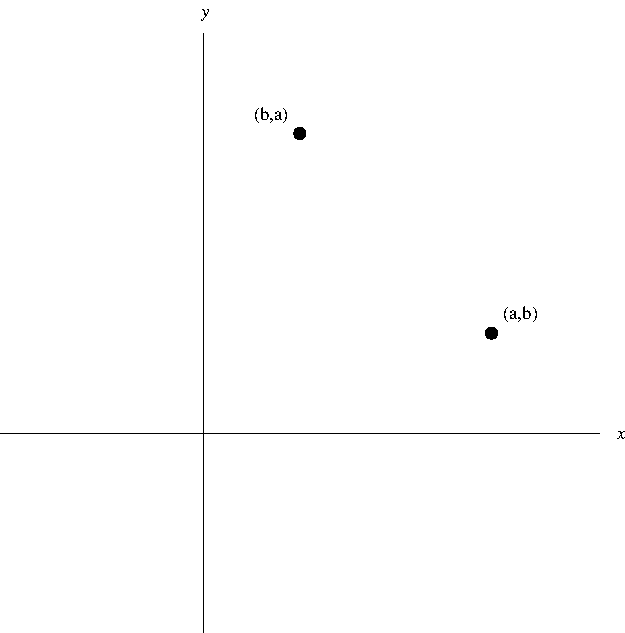
\includegraphics[height=4cm]{inverse-functions/pictures/07-01-reflectb.pdf}%
%}%
%\only<handout:1| 6->{%
%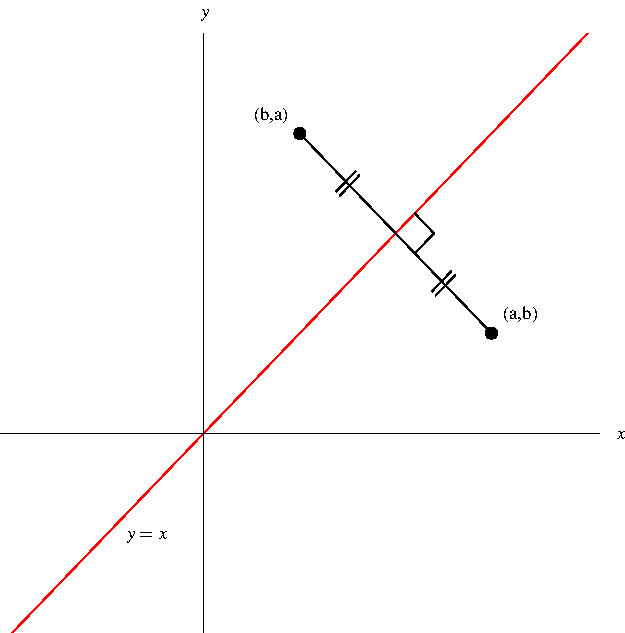
\includegraphics[height=4cm]{inverse-functions/pictures/07-01-reflectc.pdf}%
%}%
&%
\psset{xunit=0.9cm, yunit=0.9cm}
\begin{pspicture}(-1.55,-1.5)(3.5,3.2)
\psaxes[ticks=none, labels=none]{<->}(0,0)(-1.55,-1.5)(3.4,3.1)
\fcLabels{3.4}{3.1}
\uncover<7->{
\psline(0.75, 2.36359)(2.36359, 0.75)
\psline(1.65679, 1.65679)(1.55679, 1.75679)(1.45679, 1.65)
\psline(1.65679, 1.65679)(1.75679, 1.55679)(1.65679, 1.45679)
\fcFullDot{0.75}{2.36359}
\fcFullDot{2.36359}{0.75}

\psline[linecolor=blue](-1.35, -1.35)(2.8,2.8)
\rput[l](-1, -1.2){\footnotesize $y=x$}
\psplot[linecolor=red, plotpoints=1000]{-0.292893219}{3}{x 1 add ln  0.693147181 div 1 sub}
\rput[lb](0.9, 2.4){\footnotesize $y=f^{-1}(x)$}
%Function formula: 2^{1+x}-1
\psplot[linecolor=red, plotpoints=1000]{-1.5}{0.95}{-1 2 x 1 add exp add }
\psline[linecolor=blue](-1.4, -1.4)(2.9,2.9)
\rput[l](-1, -1.2){\footnotesize $y=x$}
\rput[tr](2.8, 0.4){\footnotesize $y=f(x)$}
}
\end{pspicture}
%\only<handout:0| -6>{%
%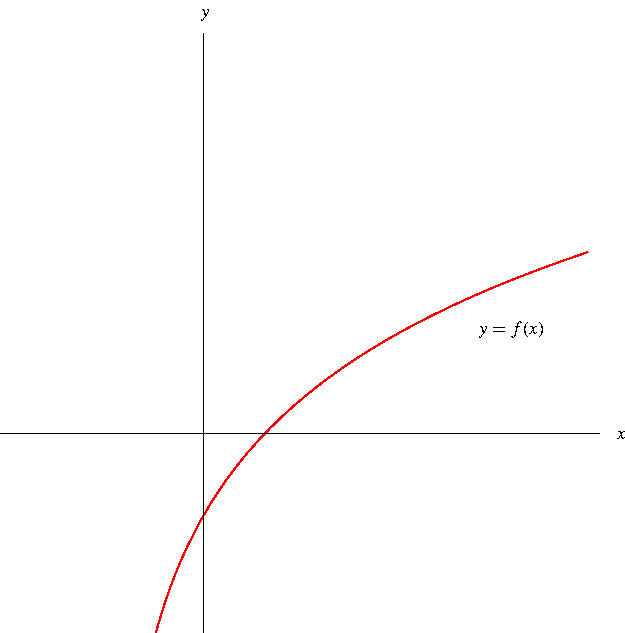
\includegraphics[height=4cm]{inverse-functions/pictures/07-01-reflect-functionb.pdf}%
%}%
%\only<handout:1| 7->{%
%\includegraphics[height=4cm]{inverse-functions/pictures/07-01-reflect-f unctiona.pdf}%
%}%
\end{tabular}

Interchanging $x$ and $y$ suggests relation between the graphs of $f^{-1}$ and $f$:
\begin{itemize}
\item<2->  Suppose $(a,b)$ is on the graph of $f$.
\item<3->  Then $f(a) = b$.
\item<4->  Then $f^{-1}(b) = a$.
\item<5->  Then $(b,a)$ is on the graph of $f^{-1}$.
\item<6->  $(b,a)$ is the reflection of $(a,b)$ in the line $y = x$.
\item<7->  Thus the graph of $f^{-1}$ is obtained by reflecting the graph of $f$ in the line $y = x$.
\end{itemize}
\end{frame}
% end module inverse-function-graph

% begin module inverse-function-ex5
\begin{frame}
\begin{example}%[Example 5, p. 388]
\begin{columns}[c]
\column{.5\textwidth}
\psset{xunit=0.5cm, yunit=0.5cm}
\begin{pspicture}(-5, -5)(5,5) 
\psframe*[linecolor=white](-5,-5)(5,5) 
\psaxes[ticks=none, labels=none]{<->}(0,0)(-4.5,-5)(4.5,5)
\psline(1, -0.1)(1, 0.1)
\rput[t](1, -0.2){\tiny$1$}
\psline(-1, -0.1)(-1, 0.1)
\psline(-0.1, 1)(0.1, 1)
\rput[br](-0.2, 1){\tiny$1$}
\psline(-0.1, -1)(0.1, -1)
\uncover<3>{
%Function formula: sqrt{}(- (x)) 
\psplot[linecolor=red, plotpoints=1000]{-4.5}{0}{x -1 mul sqrt }
\rput(-2, 2.2){\tiny$y=\sqrt{-x}$}
}
\uncover<4->{
%Function formula: sqrt{}(- (x)) 
\psplot[linecolor=gray, plotpoints=1000]{-4.5}{0}{x -1 mul sqrt }
\rput(-2, 2.2){\color{gray}\tiny$y=\sqrt{-x}$}
}
\uncover<2>{
 %Function formula: sqrt{}(x) 
\psplot[linecolor=red, plotpoints=1000]{0}{4.5}{x sqrt } 
\rput(2.4, 1){\tiny $y=\sqrt{x}$}
}
\uncover<3->{
 %Function formula: sqrt{}(x) 
\psplot[linecolor=gray, plotpoints=1000]{0}{4.5}{x sqrt } 
\rput(2.4, 1){\color{gray}\tiny $y=\sqrt{x}$}
}
\uncover<4>{
%Function formula: sqrt{}(- (x)-1) 
\psplot[linecolor=red, plotpoints=1000]{-4.5}{-1}{-1 x -1 mul add sqrt }
\rput[r](-2.3, 0.55){\tiny$y=f(x)$}
}
\uncover<5->{
%Function formula: sqrt{}(- (x)-1) 
\psplot[linecolor=gray, plotpoints=1000]{-4.5}{-1}{-1 x -1 mul add sqrt }
\rput[r](-2.3, 0.55){\color{gray}\tiny$y=f(x)$}
}

\uncover<5>{
%Function formula: - ((x)^{2})-1 
\psplot[linecolor=red, plotpoints=1000]{0}{2}{-1 x 2 exp -1 mul add } 
\rput[l](1.3, -2){\tiny$y=f^{-1}(x)$}
\psline[linecolor=blue, linestyle=dashed] (-4.5, -4.5)(4.5, 4.5)
\rput[tl](-3, -3.2){\tiny $y=x$}
}
\end{pspicture} 
%\ \only<handout:0| -1>{%
%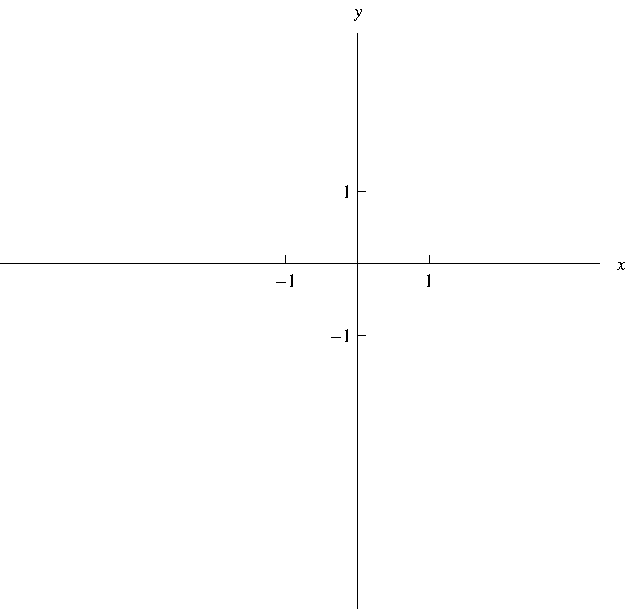
\includegraphics[height=4.5cm]{inverse-functions/pictures/07-01-ex5a.pdf}%
%}%
%\only<handout:0| 2>{%
%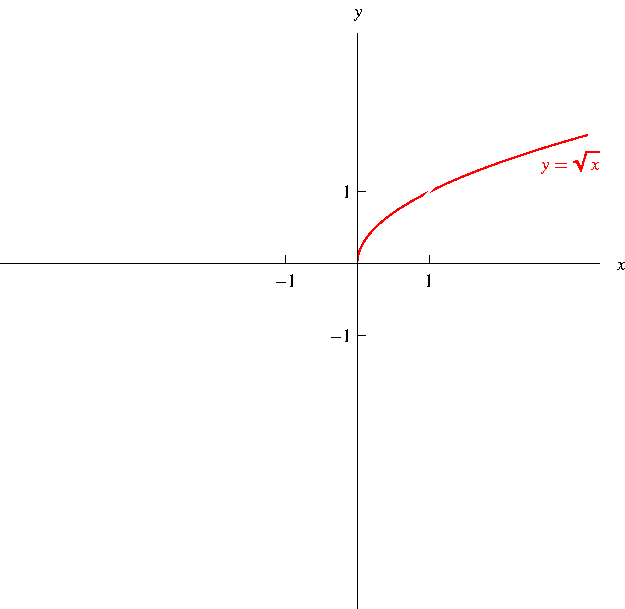
\includegraphics[height=4.5cm]{inverse-functions/pictures/07-01-ex5b.pdf}%
%}%
%\only<handout:0| 3>{%
%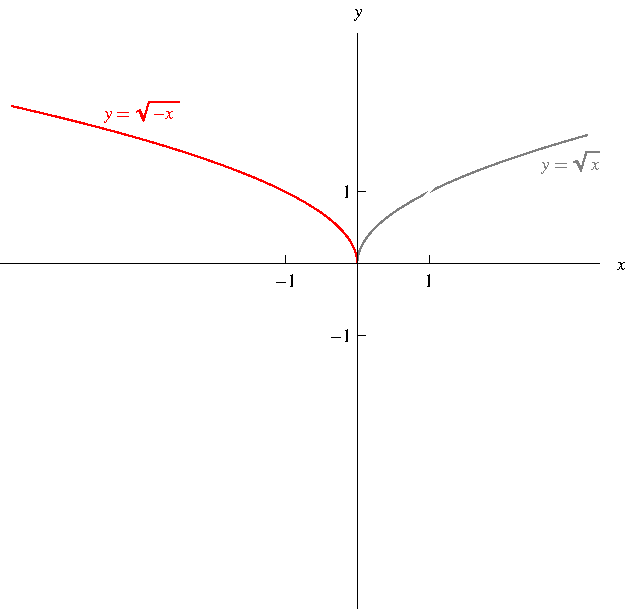
\includegraphics[height=4.5cm]{inverse-functions/pictures/07-01-ex5c.pdf}%
%}%
%\only<handout:0| 4>{%
%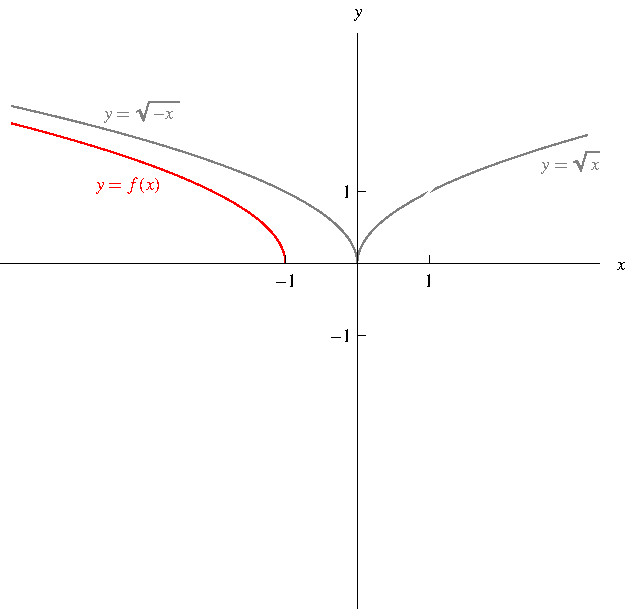
\includegraphics[height=4.5cm]{inverse-functions/pictures/07-01-ex5d.pdf}%
%}%
%\only<handout:1| 5->{%
%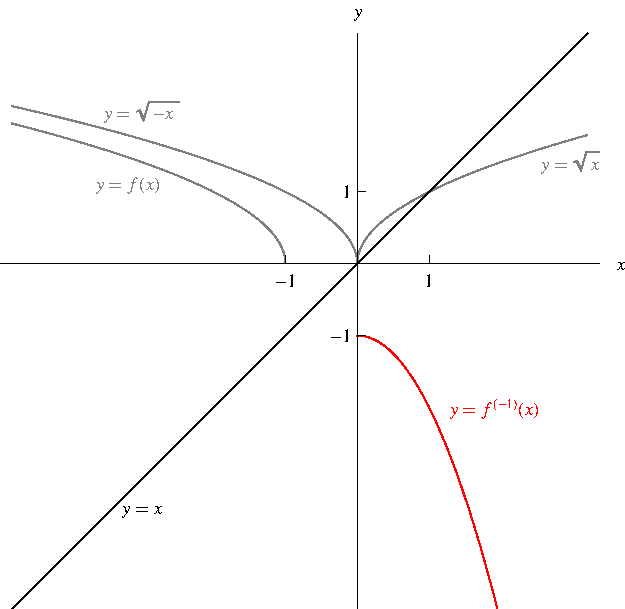
\includegraphics[height=4.5cm]{inverse-functions/pictures/07-01-ex5e.pdf}%
%}%

\column{.5\textwidth}
Sketch the graph of $f(x) = \sqrt{-x - 1}$ and its inverse function.
\end{columns}
\begin{itemize}
\item<2->  First draw the graph of $y = \sqrt{x}$.
\item<3->  $y = \sqrt{-x}$ is the reflection of $y = \sqrt{x}$ in the $y$-axis.
\item<4->  $y = f(x) = \sqrt{-x - 1}$ is the shift of $y = \sqrt{-x}$ one unit to the left.
\item<5->  $y = f^{-1}(x)$ is the reflection of $y = f(x)$ across the line $y = x$.
\end{itemize}
\end{example}
\end{frame}
% end module inverse-function-ex5
% begin module inverse-function-solve-for
\begin{frame}
%\frametitle{Inverse of a ne-to-one Function}
\begin{example}[\uncover<handout:2|16->{\alert<handout:0| 16,17>{What if we change the problem to $x\leq -\frac{2}3$?}}]
Given: $\alert<handout:0| 2>{f(x) =  3x^2+4x-7}$ \alert<handout:0| 3,16,17>{with domain $x\only<handout:1|1-16| handout:1>{\geq}\only<handout:2|17->{\leq} -\frac{2}{3}$}.  Find $f^{-1}(x)$.
\begin{columns}
\column{0.4\textwidth}
\psset{xunit=0.35cm, yunit=0.35cm}
\begin{pspicture}(-9,-9)(5,5)
\psframe*[linecolor=white](-9,-9)(5,5)
\tiny
\psaxes[ticks=none, labels=none]{<->}(0,0)(-9,-9)(4.7,4.7)
\uncover<2-16| handout:1>{ %
\psplot[linecolor=\fcColorGraph, plotpoints=1000] {-0.66}{1.401612274}{x 2 exp 3 mul x 4 mul add -7 add }
}
\uncover<handout:2|17->{ %
\psplot[linestyle=dashed, linecolor=gray!50, plotpoints=1000]{-0.66}{1.401612274}{x 2 exp 3 mul x 4 mul add -7 add }
}
\uncover<handout:2|2,17>{ %
\psplot[linecolor=\fcColorGraph, plotpoints=1000]{-2.7349}{-0.67}{x 2 exp 3 mul x 4 mul add -7 add }
}
\uncover<3-16| handout:1>{ %
\psplot[linestyle=dashed, linecolor=gray!50, plotpoints=1000] {-2.7349}{-0.67}{x 2 exp 3 mul x 4 mul add -7 add }
}
\uncover<14->{
\psline[linecolor=blue, linestyle=dashed](-6.5, -6.5)(4.5,4.5)
}
\uncover<15-16| handout:1>{
\psplot[linecolor=red, plotpoints=1000]{-8.33333}{4.5}{-0.666667 25 x 3 mul add sqrt 0.333333 mul add }
}
\uncover<handout:2|17->{
\psplot[linestyle=dashed, linecolor=gray!50, plotpoints=1000] {-8.33333}{4.5}{-0.666667 25 x 3 mul add sqrt 0.333333 mul add }
}
\uncover<handout:1|15-16>{
\psplot[linecolor=gray!50, linestyle=dashed, plotpoints=1000] {-8.33333}{4.5}{-0.666667 25 x 3 mul add sqrt -0.333333 mul add }
}
\uncover<handout:2|17->{
\psplot[linecolor=\fcColorGraph, plotpoints=1000] {-8.33333}{4.5}{-0.666667 25 x 3 mul add sqrt -0.333333 mul add }
}
\uncover<15-16| handout:1>{\rput[lb](-6, 1){$y=f^{-1}(x)$}}
\uncover<11->{\rput (-3.5, -8 ){$\left(-\frac{2}{3}, -\frac{25}{3}\right)$}}
\uncover<2-16| handout:1>{\rput[tl](1.8, 4.45){$y=f(x)$}}
\uncover<14->{\rput[l] (-7.8, -2.2 ){$\left(-\frac{25}{3}, -\frac{2}{3}\right)$}}
\uncover<handout:2|17->{\rput[rt](4.5, -3){$y=f^{-1}(x)$}}
\uncover<handout:2|17>{ \rput[tr](-3, 4.5){$y=f(x)$}}
\uncover<14->{\fcFullDot{-8.33333}{-0.666667}}
\fcFullDot{-0.666667}{-8.33333}
\end{pspicture}
\uncover<13->{Final }\uncover<12->{answer}\uncover<13->{, \alert<handout:0| 13>{relabelled}:}
\[
\uncover<12->{
f^{-1}(\only<12| handout:0>{y}\only<13->{\alert<handout:0| 13>{x}} )=-\frac{2}{3} \only<1-16| handout:1>{+} \only<handout:2|17->{\alert<handout:0| 17>{-}} \frac{\sqrt{25 +3\only<12| handout:0>{y} \only<13->{\alert<handout:0| 13>{x}}\phantom{y} }}{3}\quad.
}
\]

\column{0.6\textwidth}

\[\begin{array}{rcl}
\uncover<4->{3x^2+4x-7&=&y } \\
\uncover<4->{\alert<handout:0| 7>{3}x^2+\alert<handout:0| 6>{4}x+\alert<handout:0| 8>{(-7-y)}&=&0 }
\end{array}
\]
\uncover<5->{That's \alert<handout:0| 6,7,8>{a quadratic equation in $x$}. Solve:}
\[\begin{array}{l}
\uncover<5->{
\phantom{=}\displaystyle \frac{-\alert<handout:0| 6>{4} \pm \sqrt{\alert<handout:0| 6>{4}^2-4\cdot\alert<handout:0| 7>{3}\cdot\alert<handout:0| 8>{(-y-7)} }}{2\cdot\alert<handout:0| 7>{3}} \\
%~&=& \frac{-2 \pm \sqrt{25+3y}}{3}\\
}
\\
\uncover<9->{=\displaystyle-\frac{2 \pm \sqrt{25+3y}}{3}=} \uncover<10->{\displaystyle-\frac{2}3 \pm \frac{\sqrt{25+3y}}{3}\quad .}
\end{array}
\]
\uncover<11->{
We are given $x\only<11-16| handout:1>{\geq} \only<handout:2|17->{\alert<handout:0| 17>{\leq}}-\frac{2}3 $, therefore $x=-\frac{2}{3}\only<11-16| handout:1>{ +} \only<handout:2|17->{\alert<handout:0| 17>{-}} \frac{\sqrt{25+3y}}{3}=f^{-1}(y)$.
}
\end{columns}
\vspace{-10pt}
\end{example}
\end{frame}
% end module inverse-function-solve-for

} % end lecture

%begin lecture
\lect{January 27-31, 2014}{Lecture  3}{3}{
\section{Logarithmic Functions, Review}
% begin module logarithm-def
\begin{frame}
\frametitle{Logarithmic Functions}
\begin{columns}[c]
\column{.3\textwidth}
\psset{xunit=0.7cm, yunit=0.7cm}
\begin{pspicture}(-5, -5)(5,5) 
\psframe*[linecolor=white](-5,-5)(5,5) 
\psaxes[ticks=none, labels=none]{<->}(0,0)(-2,-2.1)(4.2, 4.2)
\psline(-0.1, 1)(0.1,1)
\rput[r](-0.2, 1){\footnotesize$1$}
\rput(0.9, 3){\footnotesize$y=a^x$}
%Function formula: 2^{x} 
\psplot[linecolor=red, plotpoints=1000]{-2}{2}{2 x exp }
\uncover<8->{
\psplot[linecolor=red, plotpoints=1000]{0.25}{4}{x ln 0.693147181 div }
\psline[linestyle=dashed, linecolor=blue](-1.9, -1.9)(4,4) 
\rput[tl](2, 0.7){\footnotesize$y=\log_ax$}
}
\end{pspicture} 
%\ \only<handout:0| -7>{%
%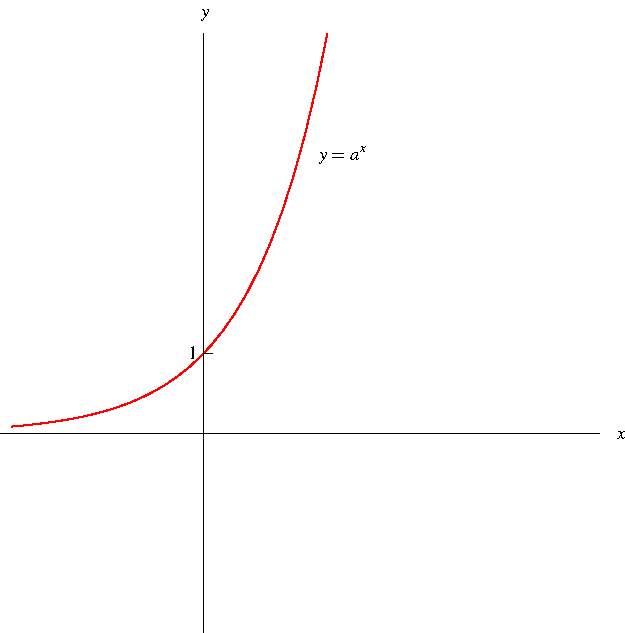
\includegraphics[height=4cm]{logarithms/pictures/07-03-logandexpa.pdf}%
%}%
%\only<8->{%
%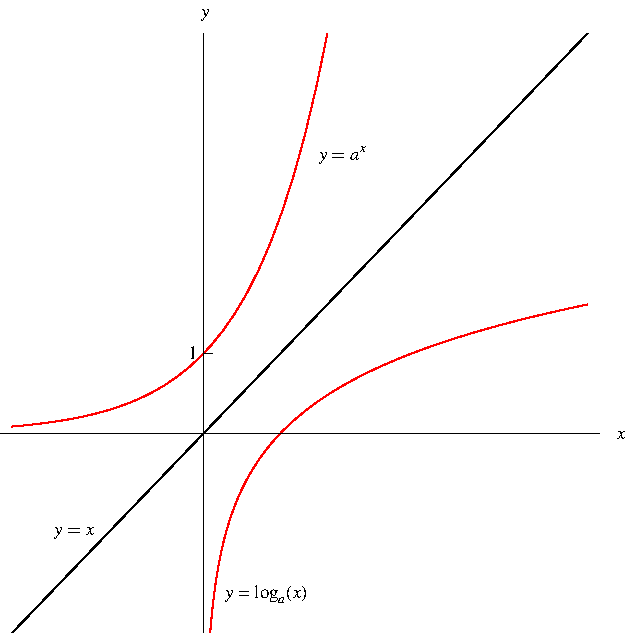
\includegraphics[height=4cm]{logarithms/pictures/07-03-logandexpb.pdf}%
%}%
\column{.7\textwidth}
\begin{itemize}
\item  Suppose $a > 0$, $a\neq 1$.
\item<2->  Let $f(x) = a^x$.
\item<3->  Then $f$ is either increasing or decreasing.
\item<4->  Therefore $f$ is one-to-one.
\item<5->  Therefore $f$ has an inverse function, $f^{-1}$.
\item<7->  The graph shows $y = a^x$ for $a > 1$.
\item<8->  The graph of $y = \log_a x$ is the reflection of this in the line $y = x$.
\end{itemize}
\end{columns}
\uncover<6->{%
\begin{definition}[$\log_a x$]
The inverse function of $f(x) = a^x$ is called the logarithmic function with base $a$, and is written $\log_a x$.  It is defined by the formula
\[
\log_a x = y \qquad \Leftrightarrow \qquad a^y = x .
\]
\end{definition}
}%
\end{frame}
% end module logarithm-def

% begin module logarithm-def-ex1
\begin{frame}
If $x > 0$, then $\log_a x$ is the exponent to which the base $a$ must be raised to give $x$.
\begin{example}%[Example 1, p. 405]
Evaluate:
\begin{enumerate}
\item<1-| alert@2-3> $\log_3 81 =$ \uncover<3->{$4$ because $3^4 = 81$.}
\item<1-| alert@4-5> $\log_{25} 5 =$ \uncover<5->{$\frac{1}{2}$ because $25^{1/2} = 5$.}
\item<1-| alert@6-7> $\log_{10} 0.001 =$ \uncover<7->{$-3$ because $10^{-3} = 0.001$.}
\end{enumerate}
\end{example}
\end{frame}
% end module logarithm-def-ex1

% begin module log-and-exp
\begin{frame}
\begin{columns}[c]
\column{.6\textwidth}
\psset{xunit=1cm, yunit=1cm}
\begin{pspicture}(-5, -5)(5,5) 
\psframe*[linecolor=white](-5,-5)(5,5) 
\psaxes[ticks=none, labels=none]{<->}(0,0)(-2,-2.1)(4.2, 4.2)
\psline(-0.1, 1)(0.1,1)
\rput[r](-0.2, 1){\footnotesize$1$}
\rput(0.9, 3){\footnotesize$y=a^x$}
%Function formula: 2^{x} 
\psplot[linecolor=red, plotpoints=1000]{-2}{2}{2 x exp }
\psplot[linecolor=red, plotpoints=1000]{0.25}{4}{x ln 0.693147181 div }
\psline[linestyle=dashed, linecolor=blue](-1.9, -1.9)(4,4) 
\rput[tl](2, 0.7){\footnotesize$y=\log_ax$}
\rput[tl](-1, -1.1){\footnotesize$y=x$}
\end{pspicture} 
%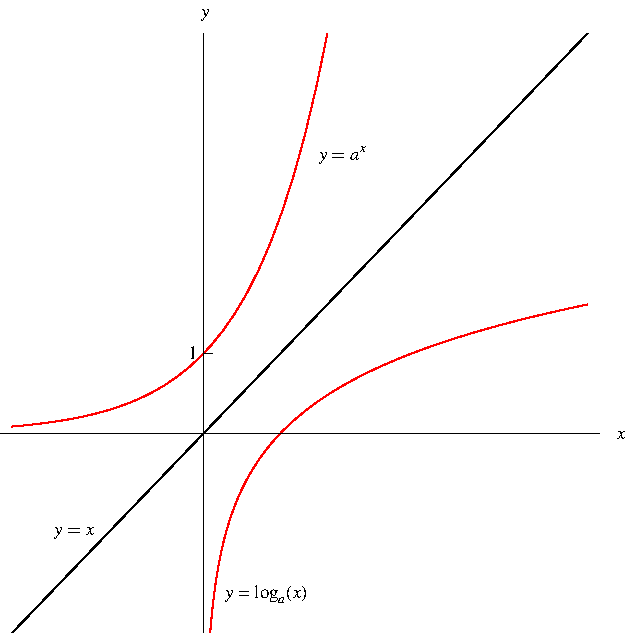
\includegraphics[height=7cm]{logarithms/pictures/07-03-logandexpb.pdf}%
\column{.4\textwidth}
\begin{itemize}
\item  Suppose $a > 1$.
\item<2-| alert@3-4>  Domain of $a^x$: \uncover<4->{$\mathbb{R}$.}
\item<2-| alert@5-6>  Range of $a^x$: \uncover<6->{$(0, \infty )$.}
\item<2-| alert@7-8>  Domain of $\log_a x$: \uncover<8->{$(0, \infty )$.}
\item<2-| alert@9-10>  Range of $\log_a x$: \uncover<10->{$\mathbb{R}$.}
\item<11->  $\log_a (a^x) = x$ for $x\in \mathbb{R}$.
\item<11->  $a^{\log_a x} = x$ for $x > 0$.
%\item<12-| alert@13-14>  $\lim_{x\rightarrow \infty}\log_a x = \uncover<14->{\infty .}$
%\item<12-| alert@15-16>  $\lim_{x\rightarrow 0^+}\log_a x = \uncover<16->{-\infty .}$
\end{itemize}
\end{columns}
\end{frame}
% end module log-and-exp

% begin module logarithm-graphs
\begin{frame}
\begin{center}
Graphs of various logarithmic functions with $a > 1$
\psset{xunit=1cm, yunit=1cm}
\begin{pspicture}(-0.5,-4.5)(7.5,3.2)
\psaxes[ticks=none, labels=none]{<->}(0,0)(-0.5,-4.5)(7.5,3.2)
\psline(1,-0.1)(1,0.1)
%Function formula: ln(x)/ln(2)
\psplot[linecolor=red, plotpoints=1000]{0.044194174}{7.5}{x ln 0.693147181 div}
\rput[r](3, 1.8){\footnotesize $y=log_2 x$}
\uncover<2->{
%Function formula: ln{x}/ln(3) 
\psplot[linecolor=black, plotpoints=1000]{0.007127781}{7.5}{x ln 1.098612289 div}
\rput[l](3.6, 1.6 ){\footnotesize $y=log_3 x$}
}
\uncover<3->{
%Function formula: ln{x}/ln(5) 
\psplot[linecolor=blue, plotpoints=1000]{0.000715542}{7.5}{x ln 1.609437912 div}
\rput[l](3.7, 1.1){\footnotesize $y=log_5 x$}
}
\uncover<4->{
%Function formula: ln{x}/ln(5) 
\psplot[linecolor=green, plotpoints=1000]{0.000031623}{7.5}{x ln 2.302585093 div}
\rput[tl](3.6, 0.6){\footnotesize $y=log_{10} x$}
}
%\rput(6, 1){\color{red!1} .}
\end{pspicture} 
%\ \only<handout:0| -1>{%
%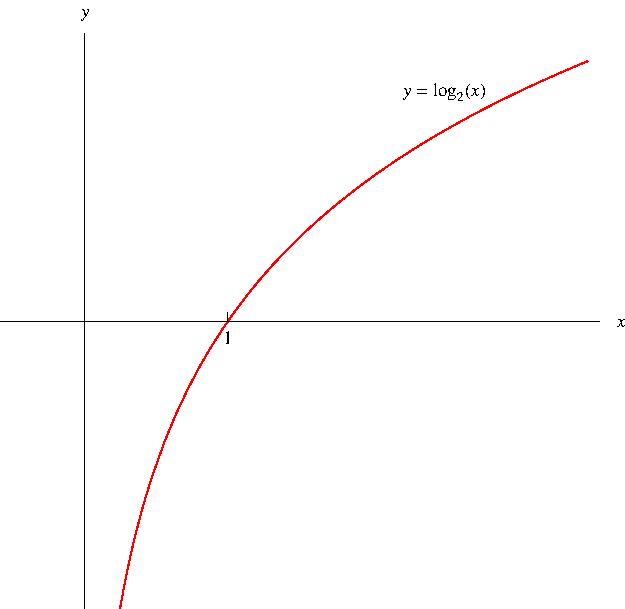
\includegraphics[height=6cm]{logarithms/pictures/07-03-manylogsa.pdf}%
%}%
%\only<handout:0| 2>{%
%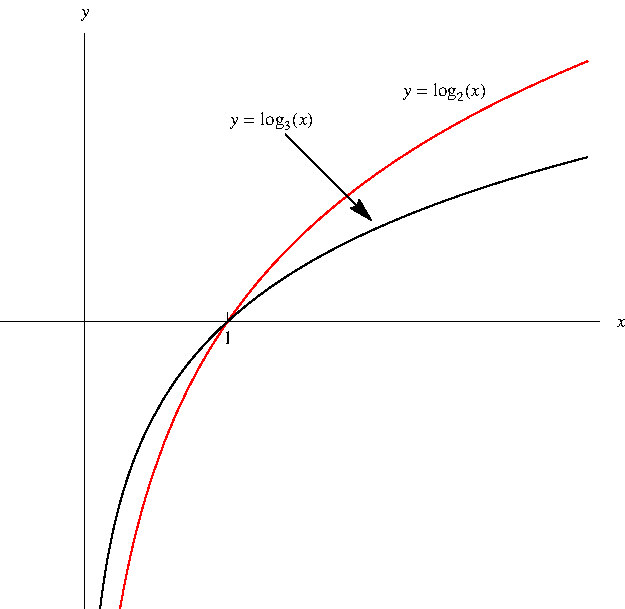
\includegraphics[height=6cm]{logarithms/pictures/07-03-manylogsb.pdf}%
%}%
%\only<handout:0| 3>{%
%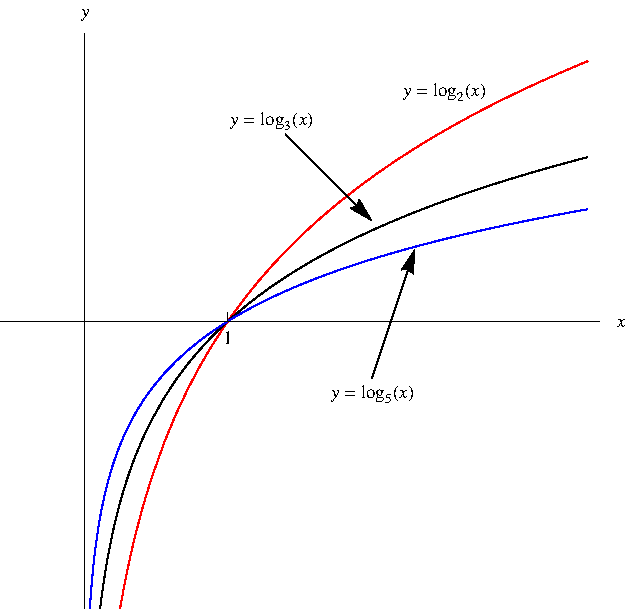
\includegraphics[height=6cm]{logarithms/pictures/07-03-manylogsc.pdf}%
%}%
%\only<4->{%
%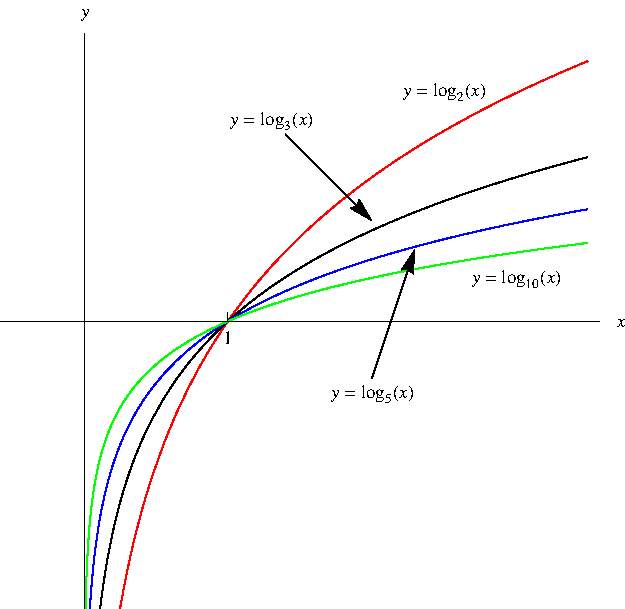
\includegraphics[height=6cm]{logarithms/pictures/07-03-manylogsd.pdf}%
%}%
\pause\pause\pause
\end{center}
\end{frame}
% end module logarithm-graphs
\subsection{Natural Logarithms}
% begin module natural-logarithm-def
\begin{frame}
\frametitle{Natural Logarithms}
\begin{definition}[$\ln x$]
The logarithm with base $e$ is called the natural logarithm, and has a special notation:
\[
\log_e x = \ln x .
\]
\end{definition}
\begin{columns}[c]
\column{.5\textwidth}
\psset{xunit=0.6cm, yunit=0.6cm}
\begin{pspicture}(-4.2,-4.2)(4.2, 4.2)
\psframe*[linecolor=white](-4.2,-4.2)(4.2, 4.2)
\psaxes[ticks=none, labels=none]{<->}(0,0)(-4.2,-4.2)(4.2, 4.2)
\psline(-0.1, 1)(0.1,1)
\rput[r](-0.2, 1){\footnotesize$1$}
\psline(1, -0.1)(1,0.1)
\rput[t](1, -0.2){\footnotesize$1$}
\rput[l](1.3, 3.2){\footnotesize$y=e^x$}
%Function formula: 2^{x} 
\psplot[linecolor=red, plotpoints=1000]{-4}{1.386294361}{2.718281828 x exp }
\psplot[linecolor=red, plotpoints=1000]{0.018315639}{4}{x ln}
\psline[linestyle=dashed, linecolor=blue](-4, -4)(4,4) 
\rput[tl](2, 0.7){\footnotesize$y=\ln x$}
\rput[tl](-2, -2.3){\footnotesize$y=x$}
\end{pspicture} 
%\ 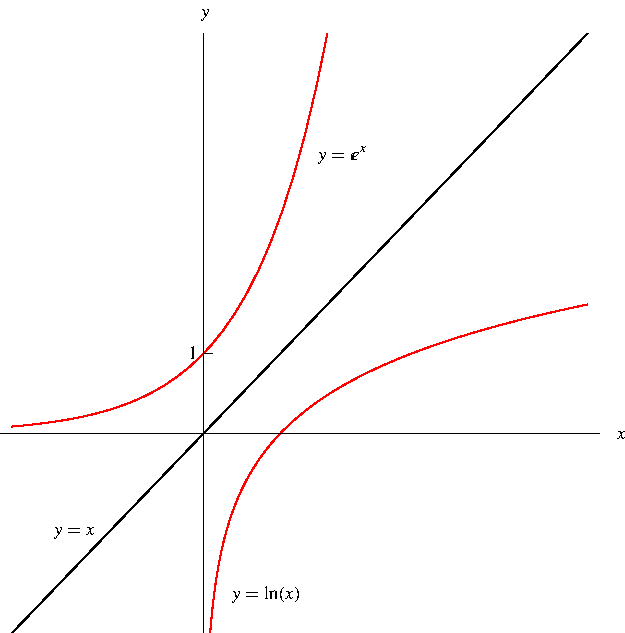
\includegraphics[height=5cm]{logarithms/pictures/07-03-natlog.pdf}%
\column{.5\textwidth}
\begin{itemize}
\item<2->  $\ln x = y \qquad \Leftrightarrow \qquad e^y = x$ .
\item<3->  $\ln (e^x ) = x$ for $x\in \mathbb{R}$.
\item<4->  $e^{\ln x}  = x$ for $x > 0$.
\end{itemize}
\end{columns}
\end{frame}
% end module natural-logarithm-def

% begin module logarithm-properties
\begin{frame}
\begin{theorem}[Properties of Logarithmic Functions]
If $a > 1$, the function $f(x) = \log_a x$ is a one-to-one, continuous, increasing function with domain $(0, \infty )$ and range $\mathbb{R}$.  If $x, y, a, b > 0$ and $r$ is any real number, then
\begin{enumerate}
\item  $\log_a (xy) = \log_a x + \log_a y$.
\item  $\log_a \left( \frac{x}{y}\right) = \log_a x - \log_a y$.
\item  $\log_a (x^r) = r\log_a x$.
\item  $\log_{a}(x)=\log_b x \log_{a} b=\frac{\log_b x}{\log_{b} a}=  \frac{\ln x}{\ln a}$.
\end{enumerate}
\end{theorem}

\end{frame}
% end module logarithm-properties

% begin module logarithm-properties-ex2
\begin{frame}
\begin{example}%[Example 2, p. 406]
Use the properties of logarithms to evaluate the following:
\begin{columns}[t]
\column{.5\textwidth}
\begin{align*}
& \invisible{=} \log_4 2 + \log_4 32 \\
&\uncover<2->{=}  \uncover<2->{\log_4 (2\cdot 32 )} \\
&\uncover<3->{=}  \uncover<3->{\log_4 (64)} \\
&\uncover<4->{=}  \uncover<4->{3} \\
& \uncover<4->{\text{(because $4^3 = 64$.)}}
\end{align*}
\column{.5\textwidth}
\begin{align*}
& \invisible{=} \log_2 80 - \log_2 5 \\
&\uncover<5->{=}  \uncover<5->{\log_2 \left( \frac{80}{5}\right) } \\
&\uncover<6->{=}  \uncover<6->{\log_2 (16)} \\
&\uncover<7->{=}  \uncover<7->{4} \\
& \uncover<7->{\text{(because $2^4 = 16$.)}}
\end{align*}
\end{columns}
\end{example}
\end{frame}
% end module logarithm-properties-ex2

% begin module logarithm-properties-ex3
\begin{frame}
\begin{example}%[Example 3, p. 406]
Find $\lim_{x\rightarrow 0} \log_{10} (\tan^2 x)$.
\begin{itemize}
\item<2->  As $x\rightarrow 0$, $t = \tan^2 x \rightarrow 0$.
\item<3->  Moreover, the values of $t$ are positive.
\item<4->  $\lim_{x\rightarrow 0} \log_{10}(\tan^2 x) = \lim_{t\rightarrow 0^+} \log_{10} t = \uncover<5->{-\infty .}$
\end{itemize}
\end{example}
\end{frame}
% end module logarithm-properties-ex3

% begin module logarithm-change-base
\begin{frame}
\frametitle{General Logarithmic and Exponential Functions}
\begin{theorem}[Logarithm Properties: Change of Base Formula]
For any positive number $a \neq 1$, we have
\[
\log_a x = \frac{\ln x}{\ln a} .
\]
\end{theorem}
\begin{proof}
\begin{itemize}
\item<2->  Let $\alertNoH{ 9-10}{y = \log_a x}$.
\item<3->  Then $a^y = x$.
\item<4->  Take the natural logarithm of both sides:
\item<5->  $\ln x=\only<7->{\alertNoH{ 7}{y \ln a}}\only<handout:0| -6>{\alertNoH{ 6}{\ln a^y}} $.
\item<8->  $\frac{\ln x}{\ln a}=\only<-9>{\alertNoH{ 9}{y}}\only<handout:0| 10->{\alertNoH{ 10}{\log_a x}} $.
\end{itemize}
\end{proof}
\end{frame}
% end module logarithm-change-base

% begin module natural-logarithm-def-ex5
\begin{frame}
\begin{example}
Solve the equation.
\[\begin{array}{rclll}
\displaystyle e^{5-3x} & =&  10 \uncover<2->{&&\text{apply }\alertNoH{2}{\ln}}\\
\uncover<2-| handout:0>{\displaystyle  \alertNoH{2,3}{\ln} ({\alertNoH{3}{e}}^{5-3x}) & =&\displaystyle  \uncover<2-| handout:0>{\alertNoH{2}{\ln} 10} } \\
\uncover<3-| handout:0>{\displaystyle \alertNoH{4}{5-}3x} & \uncover<3->{=}& \displaystyle  \uncover<3-| handout:0>{\ln 10} \\
\displaystyle \uncover<4-| handout:0>{\alertNoH{5}{3}x} & \uncover<4->{=}& \displaystyle  \uncover<4-| handout:0>{\alertNoH{4}{5-}\ln 10} \\
\displaystyle \uncover<5->{x} & \uncover<5->{=}& \displaystyle \uncover<5-| handout:0>{\frac{5-\ln 10}{\alertNoH{5}{3}}} \\
\uncover<6->{\text{Calculator:}\quad x & \approx& 0.8991.}
\end{array}
\]
\end{example}
\end{frame}
% end module natural-logarithm-def-ex5

% begin module natural-logarithm-def-ex5
\begin{frame}
\begin{example}
\text{Solve the equation}
\[
e^{2x}-3e^x-4 =  0
\]
\uncover<2->{Set $e^x=u$. \uncover<3->{Then $\alertNoH{3,4}{e^{2x}=\uncover<4->{u^2}} $.} }
\begin{align*}
\uncover<5->{u^2-3u-4 &=0} \\
\uncover<6->{\alertNoH{6,7}{\left( \uncover<7->{u-4}\right)\left(\uncover<7->{u+1}\right)} &=0}
\end{align*}
\begin{align*}
\uncover<8->{ u=4 & &\text{or} & & u=-1}\\
\uncover<8->{e^x=4  & &\text{or} & & e^x=-1}\\
\uncover<9->{x=\ln 4} \uncover<10->{& &\text{or} & &  \text{no real solution}}\\
\uncover<11->{x\approx 1.386294361 }
\end{align*}
\end{example}
\end{frame}
% end module natural-logarithm-def-ex5

% begin module natural-logarithm-def-ex5
\begin{frame}
\begin{example}
\text{Solve the equation} 
\[  
4^{x+1}+2^{x+2}-3 =  0
\]
\uncover<2->{Set $\alert<2,3>{u= \uncover<3->{2^x}}$.} \uncover<5->{Then $\alert<5,6>{4^{x+1}=\uncover<6->{4u^2} }$,} 
\uncover<7->{$\alert<7,8>{2^{x+2}=\uncover<8->{4u} }$.} 
\begin{align*}
\uncover<9->{4u^2+4u-3 &=0} \\
\uncover<10->{\alert<10,11>{4\left( \uncover<11->{u-\frac{3}2}\right)\left(\uncover<11->{u+\frac12}\right)} &=0}
\end{align*}
\begin{align*}
\uncover<12->{u=\frac32 & &\text{or} & & u=-\frac12}\\
\uncover<12->{2^x=\frac32  & &\text{or} & & 2^x=-\frac12}\\
\uncover<13->{
x=\log_2 \left(\frac32\right) =}\uncover<15->{ \frac{\alert<15,16>{\ln \uncover<16->{\frac32}} }{\alert<15,16>{\ln \uncover<16->{2}}} \uncover<17->{\approx 0.584962501} \quad  }  \uncover<14->{& &\text{or} & & \text{no real solution}}
\end{align*}
\end{example}
\end{frame}
% end module natural-logarithm-def-ex5

% begin module natural-logarithm-def-ex8
\begin{frame}
\begin{example}%[Example 8, p. 408]
Draw the graph of $y = \ln (x - 2) -1$.
\begin{columns}[c]
\column{.55\textwidth}
\psset{xunit=1cm, yunit=1cm}
\begin{pspicture}(-5, -5)(5,5) 
\psframe*[linecolor=white](-5,-5)(6,6) 
\psaxes[ticks=none, labels=none]{<->}(0,0)(-0.5,-3)(6,2.5)
\psLabelXOne
\psLabelYOne
\uncover<2>{
\psplot[linecolor=red, plotpoints=1000]{0.049787068}{6}{x ln}
\rput[lb](0.6, 0.8){\footnotesize $y=\ln(x)$}
}
\uncover<3->{
\psplot[linecolor=gray, plotpoints=1000]{0.049787068}{6}{x ln}
\rput[lb](0.6, 0.8){\color{gray}\footnotesize $y=\ln(x)$}
}
\uncover<3>{
\psplot[linecolor=red, plotpoints=1000]{2.049787068}{6}{x -2 add ln}
\rput[lb](4, 0.3){\footnotesize$y=\ln(x-2)$}
}
\uncover<4->{
\psplot[linecolor=gray, plotpoints=1000]{2.049787068}{6}{x -2 add ln}
\rput[lb](4, 0.3){\color{gray}\footnotesize$y=\ln(x-2)$}
}
\uncover<3->{
\psline[linestyle=dashed, linecolor=blue](2, -3)(2, 2.5)
\rput[l](2.1, 2){\footnotesize$x=2$}
}
\uncover<4->{
\psplot[linecolor=red, plotpoints=1000]{2.135335283}{6}{x -2 add ln -1 add}
\rput(4, -2.3){\footnotesize$y=\ln(x-2)-1$}
}

\end{pspicture} 
%\ \only<handout:0| -1>{%
%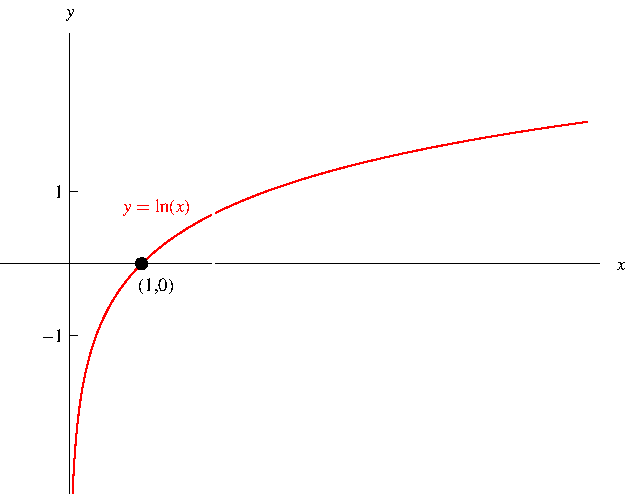
\includegraphics[height=6cm]{logarithms/pictures/07-03-ex8a.pdf}%
%}%
%\only<handout:0| 2>{%
%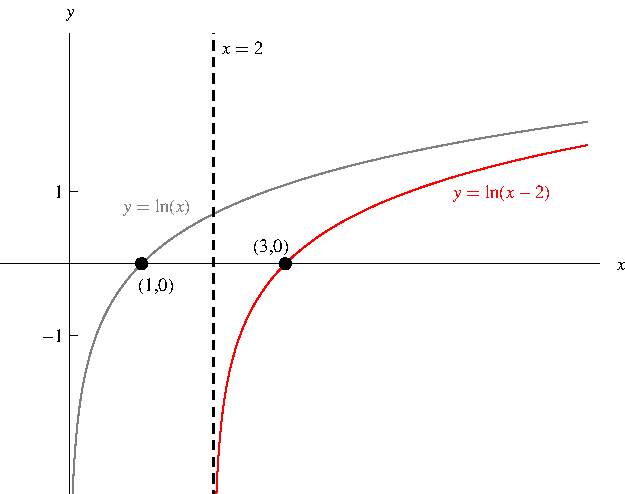
\includegraphics[height=6cm]{logarithms/pictures/07-03-ex8b.pdf}%
%}%
%\only<3->{%
%\includegraphics[height=6cm]{logarithms/pictures/07-03-ex8c.pdf}%
%}%
\column{.45\textwidth}
\begin{itemize}
\item<2-> Graph $y=\ln(x)$ assumed given.
\item<3-> $f(x-2)$ shifts graph $2$ units to the right.
\item<4-> $g(x)-1$ shifts graph $1$ unit down.
\end{itemize}
\end{columns}
\end{example}
\end{frame}
% end module natural-logarithm-def-ex8

% begin module inverse-function-solve-for
\begin{frame}
%\frametitle{Inverse of a ne-to-one Function}
\vskip -0.2cm
\begin{example}
\begin{columns}
\column{0.35\textwidth}
Find $f^{-1}(x)$ for $\displaystyle f(x) = \frac{e^x-e^{-x}}{e^x+e^{-x}}  $. 
\uncover<18->{\alertNoH{18}{$f=\tanh$ = hyperbolic tangent function.}}

\psset{xunit=0.6cm, yunit=0.6cm}
\begin{pspicture}(-3.05,-3.1)(3.15,3.2)
\psframe*[linecolor=white](-3.05,-3.1)(3.15,3.2)
\tiny
\psaxes[ticks=none, labels=none]{<->}(0,0)(-3.05,-3.1)(3.05,3.1)
\fcLabels{3.05}{3.1}
%Function formula: (679570457/250000000^{x}- (679570457/250000000^{- (x)}))/(679570457/250000000^{- (x)}+679570457/250000000^{x})
\uncover<1-16>{
\rput(-2,-0.5){$y=f(x)$}
\psplot[linecolor=\fcColorGraph, plotpoints=1000]{-3}{3}{2.71828 x -1 mul exp -1 mul 2.71828 x exp add 2.71828 x exp 2.71828 x -1 mul exp add div }
}
\uncover<17->{
\rput(-2,-0.5){$y=f(x)$}
\psplot[linecolor=gray!50, plotpoints=1000]{-3}{3}{2.71828 x -1 mul exp -1 mul 2.71828 x exp add 2.71828 x exp 2.71828 x -1 mul exp add div }
}
%Function formula: 1/2 (\ln{}((1+x)/(1- (x))))
\uncover<17->{
\psline[linestyle=dashed, linecolor=blue](-3, -3)(3,3)
\rput[tl](1.1,2.5){$y=f^{-1}(x)$}
\psplot[linecolor=\fcColorGraph, plotpoints= 1000]{ -0.994}{ 0.994 }{x 1 add x -1 mul 1 add div ln 0.5 mul }
}
\end{pspicture}
\uncover<17->{Final }\uncover<16->{answer}\uncover<17->{, \alertNoH{17}{relabeled}:}
$\displaystyle 
\uncover<16->{
f^{-1}( \only<handout:0|16>{y}\only<17->{\alertNoH{17}{x}} )=\frac12\ln\left( \frac{1+\only<handout:0|16>{y} \only<17->{ \alertNoH{17}{x}} }{1-\only<handout:0|16>{y} \only< 17->{ \alertNoH{17 }{x}}}\right)
}
$
\column{0.65\textwidth}
$ \begin{array}{@{}r@{~}c@{~}l@{}l|l}
\displaystyle \uncover<2->{ \frac{ \alertNoH{3}{e^x}- \alertNoH{4, 5}{e^{-x} } }{ \alertNoH{3}{e^x}+\alertNoH{4,5}{e^{-x}}} &=&y\uncover<3->{ &&\begin{array}{l} \text{Set } \alertNoH{3, 12}{u=e^x} \\\uncover<4->{ \alertNoH{4, 5}{e^{-x}=} \fcAnswer{5}{\frac{1}{e^x}= \frac{1}{u}}} \end{array}}}  \\
\displaystyle\uncover<3->{ \frac{ \left(\alertNoH{3}{ u} -\fcAnswerUncover{3}{5}{\frac{1}{u}}\right)\uncover<6->{\alertNoH{6}{u}} }{\left( \alertNoH{3}{u}+ \fcAnswerUncover{3}{5}{\frac{1}{u}}\right)\uncover<6->{\alertNoH{6}{u}}}&=&y}\\
\displaystyle\uncover<7->{\frac{u^2-1}{\alertNoH{8}{u^2+1}}&=&y}\\
\displaystyle\uncover<8->{ \alertNoH{9}{u^2}- \alertNoH{10}{1} &=&\alertNoH{9,10}{ y}( \alertNoH{8}{ \alertNoH{9}{u^2} +\alertNoH{10 }{1}})}\\
\displaystyle\uncover<9->{\alertNoH{9}{ u^2(\alertNoH{11}{1-y})}&=&\alertNoH{10} {1+y}}\\
\displaystyle\uncover<11->{ {\alertNoH{12}{u}}^2&=&\displaystyle \frac{1+y}{ \alertNoH{11}{1-y} }}\\
\displaystyle \uncover<12->{\left(\alertNoH{12}{e^{\alertNoH{13}{x}}} \right)^{\alertNoH{13}{2}}&=&\displaystyle \frac{1+y}{1-y}}\\
\uncover<13->{\displaystyle e^{\alertNoH{13}{2x}}&=&\displaystyle \frac{1+y}{1-y}}\uncover<14->{ &&\text{Take }\alertNoH{14}{\ln}} \\
\uncover<14->{\displaystyle \uncover<handout:0|14,15>{ \alertNoH{15}{2}} x&=&\displaystyle \uncover<16->{ \alertNoH{16}{\frac{1}{2}}} \alertNoH{14}{\ln} \left(\frac{1+y}{1-y} \right)}\\
\end{array}
$
\end{columns}
\vskip -0.3cm
\end{example}
\end{frame}
% end module inverse-function-solve-for

\section{Derivatives of Logarithms, Review}
\subsection{The Natural Logarithm}
% begin module natural-logarithm-derivative
\begin{frame}
\frametitle{The Derivative of the Natural Logarithm}
\begin{theorem}[The Derivative of $\ln x$]
\[
\frac{\diff}{\diff x} (\ln x) = \frac{1}{x} .
\]
\end{theorem}
\begin{proof}
\begin{itemize}
\item<2->  Let $\alertNoH{ 8,10}{y = \ln x}$.
\item<3->  Then $e^y = x$.
\item<4->  Differentiate this implicitly with respect to $x$:
\item<5->  $e^y \frac{\diff y}{\diff x} = 1$.
\item<6->  Rearrange:
\item<7->  $\uncover<10->{\frac{\diff}{\diff x} (\alertNoH{ 10}{\ln x}) = } \frac{\diff \alertNoH{ 10}{y}}{\diff x} = \frac{1}{e^{\alertNoH{ 8}{y}}} \uncover<8->{ = \frac{1}{e^{\alertNoH{ 8}{\ln x}}}} \uncover<9->{ = \frac{1}{x}.}$
\end{itemize}
\end{proof}
\end{frame}
% end module natural-logarithm-derivative

% begin module natural-logarithm-derivative-ex1
\begin{frame}
\chainruley{\ln (x^3+1)}{x^3+1}{\ln u}{\frac{1}{UU}}{3x^2}{\frac{3x^2}{UU}}{ %Example 1, p. 222
}
\end{frame}
% end module natural-logarithm-derivative-ex1

% begin module general-logarithm-derivative
\begin{frame}
\frametitle{General Logarithmic and Exponential Functions}
\begin{theorem}[The Derivative of $\log_a$]
\[
\frac{\diff}{\diff x} (\log_a x) = \frac{1}{x\ln a} .
\]
\end{theorem}
%\begin{theorem}[The Derivative of $a^x$]
%\[
%\frac{\diff}{\diff x} (a^x) = a^x \ln a .
%\]
%\end{theorem}
\begin{proof}
\uncover<2->{Since $\ln a$ is a constant, we can differentiate as follows:}
\[
\uncover<3->{\frac{\diff}{\diff x} (\log_a x) =}%
\uncover<4->{\frac{\diff}{\diff x} \frac{\ln x}{\ln a} = }%
\uncover<5->{\frac{1}{\ln a} \frac{\diff}{\diff x} (\ln x) = }%
\uncover<6->{\frac{1}{x \ln a}.}%
\]
\end{proof}
\end{frame}
% end module general-logarithm-derivative

% begin module general-logarithm-derivative-ex12
\begin{frame}
\chainruley{\log_{10} (2+\sin x)}{2+\sin x}{\log_{10} u}{\frac{1}{UU\ln 10}}{\cos x}{\frac{\cos x}{(UU)\ln 10}}{Example 4, p. 222}
\end{frame}
% end module general-logarithm-derivative-ex12

\subsection{The Number $e$ as a Limit}
% begin module e-limit
\begin{frame}
\begin{theorem}[The Number $e$ as a Limit]
\[
e = \lim_{x\rightarrow 0} (1 + x)^{\frac{1}{x}} = \lim_{y\to \infty} \left(1+\frac{1}{y}\right)^y.
\]
\end{theorem}
\begin{proof}
\uncover<2->{Let $f(x) = \ln x$.  }%
\uncover<3->{Then $f'(x) = \frac{1}{x}$, so $f'(1) = 1$.}%
\abovedisplayskip=0pt
\belowdisplayskip=0pt
\abovedisplayshortskip=0pt
\belowdisplayshortskip=0pt
\begin{align*}
\uncover<4->{\alertNoH{ 10}{1} = f'(1)} & \uncover<4->{=} %
\uncover<4->{\lim_{h\rightarrow 0}\frac{f(1+h)-f(1)}{h}}%
\uncover<5->{ = \lim_{x\rightarrow 0}\frac{f(1+x)-f(1)}{x}}\\%
& \uncover<6->{=}  %
\uncover<6->{\lim_{x\rightarrow 0}\frac{\ln (1+x)-\ln (1)}{x}}%
\uncover<7->{ = \lim_{x\rightarrow 0}\frac{1}{x}\ln (1 + x)}\\%
& \uncover<8->{\alertNoH{ 10}{=}}  %
\uncover<8->{\alertNoH{ 10}{\lim_{x\rightarrow 0}\ln (1+x)^{\frac{1}{x}}}.}
\end{align*}
\uncover<9->{Then use the fact that \alertNoH{ 11}{the exponential function is continuous}:}
\[
\uncover<9->{e = e^{\alertNoH{ 10}{1}} =}%
\uncover<10->{\alertNoH{ 11}{e^{\alertNoH{ 10}{\lim\limits_{x\rightarrow 0}\ln (1+x)^{\frac{1}{x}}}} =}}%
\uncover<11->{\alertNoH{ 11}{\lim\limits_{x\rightarrow 0}e^{\ln (1+x)^{\frac{1}{x}}}} =}%
\uncover<12->{\lim\limits_{x\rightarrow 0} (1+x)^{\frac{1}{x}}.}\qedhere
\]
\end{proof}
\end{frame}
% end module e-limit

%begin module e-limit-problems-ex1
\begin{frame}
\begin{example}
Compute
\[
\begin{array}{rcll|l}
\displaystyle\lim\limits_{x\to \infty}\left(\alertNoH{2}{ \frac{x+3}{x}} \right)^x
\uncover<2->{
&=&\displaystyle  \lim\limits_{x\to \infty} \left(\alertNoH{2}{1 +\alertNoH{3}{\frac{3}{x}} } \right)^{\alertNoH{4}{x}} } \\
\uncover<3->{&=& \displaystyle \lim\limits_{x\to \infty}\left(1+\frac{1}{\alertNoH{3,6}{ \frac{x}{3}} }\right)^{\alertNoH{4}{3\alertNoH{6}{\frac{x}{3}}} } } \uncover<5->{ && \text{Set } \alertNoH{6}{\frac{x}{3}=y}}\\
\uncover<6->{&=&\displaystyle \lim\limits_{\substack{\alertNoH{7}{x\to \infty} \\ \uncover<7->{\alertNoH{7}{\frac{x}{3}=y\to \infty} } }}\left(1+\frac{1}{\alertNoH{6}{y}}\right)^{\alertNoH{8}{3\alertNoH{6}{y}}} } \\
\uncover<8->{ &=&\displaystyle \alertNoH{9,10}{ \alertNoH{11}{\lim\limits_{y\to \infty}}\left(\alertNoH{11}{\left(1+\frac{1}{y}\right)^{\alertNoH{8}{y}}}\right)^{\alertNoH{8}{3}}}} \uncover<9->{\alertNoH{9,10}{=}}\uncover<10->{\alertNoH{10}{\alertNoH{11}{ e}^3} \quad .}
\end{array}
\]

\end{example}
\end{frame}
\begin{frame}
\begin{example}
Compute
\[
\begin{array}{rll|l}
&\displaystyle \lim_{x\to \infty} \left(\frac{\alertNoH{2}{x}}{x-2} \right)^{2x+2}\\
\uncover<2->{ =&\displaystyle
\lim\limits_{x\to \infty}\left(\alertNoH{3}{ \frac{\alertNoH{2}{x-2 +2}} {x-2} } \right)^{2x+2}}
\uncover<3->{= \lim\limits_{x\to \infty}\left(\alertNoH{3}{1+\alertNoH{4}{\frac{2}{x-2}} } \right)^{2\alertNoH{5}{x}+2}} \\
\uncover<4->{=&\displaystyle \lim\limits_{x\to \infty} \left( 1+ \alertNoH{4}{\frac{1}{ \frac{x-2}{2}}} \right)^{\alertNoH{6}{ 2( \alertNoH{5}{ x-2+2} )+2}} }\\
\uncover<6->{ =&\displaystyle \lim\limits_{x\to \infty} \left( 1+ \frac{1}{ \alertNoH{8}{ \frac{x-2}{2}} } \right)^{ \alertNoH{6}{ 4\alertNoH{8}{\frac{x-2}{2}} +6}}} \uncover<8->{= \lim \limits_{\substack{ \alertNoH{8}{\frac{ x-2 }{2}
= y} \\ y\to\infty}} {\alertNoH{9,10}{\left(1+\frac{1}{\alertNoH{8}{ y} }\right)}}^{\alertNoH{9}{4\alertNoH{8}{y}} +\alertNoH{10}{6}} } \uncover<7->{&& \alertNoH{7}{\text{Set } \alertNoH{8}{y=\frac{x-2}{2}} }}\\
\uncover<9->{=& \displaystyle \alertNoH{12}{ \lim\limits_{y\to \infty} }  \alertNoH{9}{ \left( \alertNoH{12}{\left(1+\frac{1}{y} \right)^{y}}\right)^4} \alertNoH{13}{\lim\limits_{ y\to\infty}} \alertNoH{10}{\left(1+\alertNoH{13}{\frac{1}{y}} \right)^6} } \\ \uncover<11->{ =&\alertNoH{14}{ \alertNoH{12}{e}^4\cdot (1+\alertNoH{13}{0})^6}}\uncover<14->{
= \alertNoH{14}{e^4} \quad . }
\end{array}
\]

\end{example}
\end{frame}
%end module e-limit-problems-ex1

\subsection{Derivatives of Exponents with Arbitrary Base}
% begin module general-exponential-derivative
\begin{frame}
\begin{theorem}[The Derivative of $a^x$]
\[
\frac{\diff}{\diff x} (a^x) = a^x \ln a .
\]
\end{theorem}
\begin{proof}
\uncover<2->{
Use the fact that $\alert<handout:0| 4,8>{a = e^{\ln a}}$.
}
\begin{eqnarray*}
\uncover<3->{\frac{\diff}{\diff x} (\alert<handout:0| 4>{a^x})}%
& \uncover<3->{ = } & %
\uncover<4->{\frac{\diff}{\diff x} (\alert<handout:0| 4>{e^{\ln a}})^x}\\%
& \uncover<5->{ = } & %
\uncover<5->{\frac{\diff}{\diff x} e^{(\ln a)x}}\\%
& \uncover<6->{ = } & %
\uncover<6->{ e^{(\ln a)x}\frac{\diff}{\diff x}(\ln a)x }\\%
& \uncover<7->{ = } & %
\uncover<7->{ (\alert<handout:0| 8>{e^{\ln a}})^x(\ln a) }\\%
& \uncover<8->{ = } & %
\uncover<8->{ \alert<handout:0| 8>{a}^x(\ln a).}%
\end{eqnarray*}
\end{proof}
\end{frame}
% end module general-exponential-derivative

% begin module general-exponential-derivative-ex13
\begin{frame}
\chainruley{10^{x^2}}{x^2}{10^u}{10^{UU}(\ln 10)}{2x}{(2\ln 10)x10^{UU}}{Example 13, p. 416}
\end{frame}
% end module general-exponential-derivative-ex13

\subsection{Derivatives of Arbitrary Exponents with Arbitrary Base}
\begin{frame}
\begin{example}
Compute $\frac{\diff}{\diff x} \left((\tan x)^{\frac{1}{x}} \right)$,  where $x\in (0,\frac{\pi}{2})$.

\[
\begin{array}{rcl}
\uncover<2->{\displaystyle  \frac{\diff }{\diff x} \left((\alertNoH{3}{\tan x})^{\frac{1}{x}} \right)&=&} \uncover<3->{ \displaystyle \frac{\diff }{\diff x} \left( (\alertNoH{3}{e^{\alertNoH{4}{\ln \tan x} }})^{ \alertNoH{4}{\frac{1}{x}} } \right)}  \uncover<4->{=\frac{\diff }{\diff x} \left( e^{\alertNoH{4}{\frac{1}{x}\ln \tan x}} \right)}\\
\uncover<5->{ &=&\displaystyle  \alertNoH{6}{e^{\frac{1}{x} \ln (\tan x)}} \alertNoH{7,8}{\frac{\diff }{\diff x}\left(\frac{1}{x} \ln( \tan x) \right)}} \\
\uncover<6->{&=&\displaystyle  \alertNoH{6}{ (\tan x)^{\frac{1}{x}}}\alertNoH{7,8}{ \left( \uncover<8->{ -\frac{1}{x^2} \ln (\tan x) +\frac{1}{x} \frac{(\tan x)' }{\tan x}}\right)}} \\
\uncover<9->{&=&\displaystyle (\tan x)^{\frac{1}{x}} \left( -\frac{1}{x^2} \ln (\tan x) +\frac{1}{x} \frac{\frac{1}{\cos^2(x)}}{\frac{\sin x}{\cos x}}\right)}\\
\uncover<10->{&=&\displaystyle (\tan x)^{\frac{1}{x}} \left( -\frac{1}{x^2} \ln (\tan x) +\frac{1}{x} \frac{1}{\sin x \cos x}\right)}
\end{array}
\]
\end{example}

\end{frame}

% begin module arbitrary-base-arbitrary-exponent-derivative
\begin{frame}
\begin{example}
Suppose $g(x)$ and $f(x)$ are differentiable functions and suppose $g(x)>0$. Prove that
\[
\frac{d}{dx} \left(g(x)^{f(x)} \right)=g(x)^{f(x)} \left( f'(x) \ln (g(x)) + f(x)\frac{g'(x)}{g(x)}\right) \quad .
\]
\end{example}
\begin{proof}
\[
\begin{array}{rcl}
\displaystyle \frac{d}{dx} \left(g(x)^{f(x)} \right)&=&\displaystyle \frac{d}{dx} \left( \left(e^{\ln g(x)}\right)^{f(x)} \right)=\frac{d}{dx} \left(e^{f(x)\ln g(x)} \right)\\
&=&\displaystyle e^{f(x)\ln g(x)} \frac{d}{dx} (f(x) \ln g(x)) \\
&=&\displaystyle 
g(x)^{f(x)} \left( f'(x) \ln (g(x)) + f(x)\frac{g'(x)}{g(x)}\right)\quad ,
\end{array}
\]
as desired.
\end{proof}
\end{frame}
%end module arbitrary-base-arbitrary-exponent-derivative
} %end lecture

% begin lecture
\lect{February 3-7, 2014}{Lecture  4}{4}{
\section{Inverse Trigonometric Functions}
% begin module arcsin-def
\begin{frame}
\frametitle{Inverse Trigonometric Functions}
\psset{xunit=0.6cm,yunit=0.6cm}
\begin{pspicture}(-5,-1.4)(10,1.4)
\tiny
\psaxes[labels=none, Dx=1.570796327, Dy=1] {<->}(0,0)(-4,-1.8)(10,1.8)

\uncover<1-2| handout:0>{\psplot[linecolor=red, plotpoints=1000]{-4}{10}{x 57.295779513 mul sin}}
\uncover<2| handout:0>{\psline(-4,0.6)(10,0.6 )}

\uncover<3>{\psplot[linecolor=red, plotpoints=1000]{-1.570796327}{1.570796327}{x 57.295779513 mul sin}
\rput[bl](3, 1){\alert<3>{$y=\sin x, -\frac{\pi}{2}\leq x\leq \frac{\pi}{2}$} }
}
\uncover<4-| handout:0>{\psplot[linecolor=gray, plotpoints=1000]{-1.570796327}{1.570796327}{x 57.295779513 mul sin}
\rput[bl](3, 1){\color{gray}{$y=\sin x, -\frac{\pi}{2}\leq x\leq \frac{\pi}{2}$} }
}

\uncover<4-| handout:0>{\psplot[linecolor=red, plotpoints=1000]{-1}{1}{x ASIN}
\rput[r](-1.5, -1){\alert<4>{$y=\Arcsin x$} }

}

\rput[t](-3.14, -0.3){$-\pi$}
\rput[t](-1.57, -0.3){$-\frac{\pi}{2}$}
\rput[t](1.57, -0.3){$\frac{\pi}{2}$}
\rput[t](3.14, -0.3){$\pi$}
\rput[t](4.71, -0.3){$\frac{3\pi}{2}$}
\rput[t](6.28, -0.3){$2\pi$}
\rput[t](7.85, -0.3){$\frac{5\pi}{2}$}
\rput[t](9.42, -0.3){$3\pi$}
\rput[bl](0.2,1){\tiny $1$}
\end{pspicture}
\begin{columns}[c]
\column{.65\textwidth}
\begin{itemize}
\item<2->  $\sin x$ isn't one-to-one.
\item<3->  It is if we restrict the domain to $\left[-\frac{\pi}{2}, \frac{\pi}{2}\right]$.
\item<4->  Then it has an inverse function.
\item<4->  We call it $\arcsin$ or $\sin^{-1}$.
\item<6->  $\Arcsin x = y \Leftrightarrow \sin y = x$ and $-\frac{\pi} {2} \leq y \leq \frac{\pi}{2}$.
\end{itemize}
\column{.35\textwidth}
\psset{xunit=1cm,yunit=1cm}
\uncover<5->{
\begin{pspicture}(-1.5,-2)(1.7,2)
\tiny
\psaxes[ticks=none, labels=none]{<->}(0,0)(-1.5,-2)(1.5,2)
\fcLabels{1.5}{2}
\fcLabelXOne
\psline(-1, -0.1)(-1,0.1)
\rput[t](-1,  -0.1){$-1$}

\psline(-0.1, 1.570796327)(0.1,1.570796327)
\rput[r](-0.1,  1.570796327){$\frac{\pi}{2}$}
\psline(-0.1, -1.570796327)(0.1,-1.570796327)
\rput[r](-0.1,  -1.570796327){$-\frac{\pi}{2}$}

\psplot[linecolor=red, plotpoints=1000]{-1}{1}{x ASIN}
\rput[rb](-0.05, 0.2){\alert<4>{$y=\Arcsin x$} }
\fcFullDot{1}{1.570796327}
\fcFullDot{-1}{-1.570796327}
\end{pspicture}
}
%\uncover<5->{%
%\includegraphics[height=4cm]{inverse-trig/pictures/07-06-arcsine.pdf}%
%}%

\end{columns}
\end{frame}
% end module arcsin-def

% begin module arcsin-ex1
\begin{frame}
\begin{example} %[Example 1, p. 217]
\begin{columns}[t]
\column{.4\textwidth}
\[
\text{Find } \ \Arcsin \left( \frac{1}{2}\right)
\]
\begin{itemize}
\item<2->  $\sin (\uncover<2-| handout:0>{\frac{\pi}{ 6}}) = \frac{1}{2}$.
\item<3->  $-\frac{\pi}{2} \leq \uncover<3-| handout:0>{\frac{\pi}{6}} \leq \frac{\pi}{2}$.
\item<4->  Therefore $\Arcsin \left( \frac{1}{2}\right) = \uncover<3-| handout:0>{\frac{\pi}{6}}$.
\end{itemize}
\column{.6\textwidth}
\[
\text{Find } \ \tan \left( \Arcsin \left( \frac{1}{3}\right) \right)
\]
\begin{itemize}
\item<5->  Let $\theta = \Arcsin (1/3)$, so $\sin \theta = 1/3$.
\item<6->  Draw a right triangle with opposite side $1$ and hypotenuse $3$.
\item<7->  \alert<handout:0| 7-8>{Length of adjacent side $ = \uncover<8-| handout:0>{\sqrt{3^2-1^2} = \sqrt{8} = 2\sqrt{2}.}$}
\item<9->  Then \alert<handout:0| 9-10>{$\tan (\Arcsin \frac13) = \uncover<10-| handout:0>{\frac{1}{2\sqrt{2}}.}$}
\end{itemize}

\psset{xunit=1.8cm, yunit=1.8cm}
\begin{pspicture}(-0.2, -0.35)(3.2,1.05)
\psframe*[linecolor=white](-0.2, -0.35)(3.3,1.05)
\psline[linecolor=red!1](2.828427125, 1)(2.828427125, 1.01)
\psline[linecolor=red!1](0, -0.35)(0.001, -0.35)
\uncover<5->{\psline(0,0)(2.828427125, 0)(2.828427125, 1)(0,0)
\psline(2.828427125, 0.1)(2.728427125, 0.1)(2.728427125,0)
\rput[b](1.41, 0.55){$3$}
\rput[l](2.87, 0.5){$1$}
\rput(0.55, 0.1){$\theta$}
\fcAngle{0}{0.339837}{0.4}{}
}
\uncover<7>{\rput[t](1.41, -0.1){\alert<7| handout:0>{?}} }
\uncover<8-| handout:0>{\rput[t](1.41, -0.1){\alert<8>{$2\sqrt{2}$}} }

\end{pspicture}


\end{columns}
\end{example}
\end{frame}
% end module arcsin-ex1

% begin module arcsin-derivative
\begin{frame}
\begin{theorem}[The Derivative of $\sin^{-1} x$]
\[
\frac{\diff}{\diff x} \left( \sin^{-1} x\right) = \frac{1}{\sqrt{1-x^2}} \qquad -1 < x < 1.
\]
\end{theorem}
\begin{proof}
\begin{itemize}
\item  $\sin$ is differentiable, so $\sin^{-1}$ is too.
\item<2->  Let $y = \sin^{-1} x$.  Then $\alert<handout:0| 3,7>{\sin y = x}$ and $\alert<handout:0| 8>{-\pi /2 \leq y \leq \pi /2}$.
\item<3->  Differentiate implicitly with respect to $x$:
\item<4->  $\cos y \frac{\diff y}{\diff x} = 1$.
\item<5->  $ \frac{\diff y}{\diff x} = \frac{1}{\cos y}$.
\item<6->  \uncover<8->{\alert<handout:0| 8>{$\cos y \geq 0$}, so} $\alert<handout:0| 11>{\cos y =} \only<handout:0| -8>{\alert<handout:0| 8>{\pm}}\sqrt{1 - \alert<handout:0| 7>{\sin^2 y}} \uncover<7->{ = \only<handout:0| -8>{\alert<handout:0| 8>{\pm}}\alert<handout:0| 11>{\sqrt{1-\alert<handout:0| 7>{x^2}}}.}$
\item<10->  $ \frac{\diff y}{\diff x} = \frac{1}{\alert<handout:0| 11>{\cos y}} \uncover<11->{ = \frac{1}{\alert<handout:0| 11>{\sqrt{1-x^2}}}.\qedhere}$
\end{itemize}
\end{proof}
\end{frame}
% end module arcsin-derivative

% begin module arcsin-properties
\begin{frame}
Important facts about $\Arcsin$:
\begin{columns}[c]
\column{.5\textwidth}
%\ \includegraphics[height=6cm]{inverse-trig/pictures/07-06-arcsine.pdf}%
\psset{xunit=2cm,yunit=2cm}
\begin{pspicture}(-5,-1.4)(10,1.4)
\tiny
\psaxes[ticks=none, labels=none]{<->}(0,0)(-1.5,-2)(1.5,2)
\psLabels{1.5}{2}
\psLabelXOne
\psline(-1, -0.1)(-1,0.1)
\rput[t](-1,  -0.1){$-1$}

\psline(-0.1, 1.570796327)(0.1,1.570796327)
\rput[r](-0.1,  1.570796327){$\frac{\pi}{2}$}
\psline(-0.1, -1.570796327)(0.1,-1.570796327)
\rput[r](-0.1,  -1.570796327){$-\frac{\pi}{2}$}

\psplot[linecolor=red, plotpoints=1000]{-1}{1}{x ASIN}
\rput[rb](-0.05, 0.2){$y=\Arcsin x$} 
\psFullDot{1}{1.570796327}
\psFullDot{-1}{-1.570796327}
\uncover<3>{\psline[linecolor=red, linewidth=2pt]{<->}(-1,0)(1,0) }
\uncover<5>{\psline[linecolor=red, linewidth=2pt]{<->}(0,-1.570796327)(0,1.570796327) }

\end{pspicture}
\column{.5\textwidth}
\begin{enumerate}
\item  \alert<handout:0| 2-3>{Domain: \uncover<3->{$[-1, 1]$.}}
\item  \alert<handout:0| 4-5>{Range: \uncover<5->{$[-\pi /2, \pi /2]$.}}
\item  $\Arcsin x = y \Leftrightarrow \sin y = x$ and $-\pi /2 \leq y \leq \pi /2$.
\item  $\Arcsin (\sin x) = x$ for $-\pi /2 \leq x \leq \pi /2$.
\item  $\sin (\Arcsin x) = x$ for $-1 \leq x \leq 1$.
\item  $\frac{\diff}{\diff x} (\Arcsin x) = \frac{1}{\sqrt{1-x^2}}$.
\end{enumerate}
\end{columns}
\end{frame}
% end module arcsin-properties


% begin module arccos-def
\begin{frame}
%\ \only<handout:0| -1>{%
%\includegraphics[width=12cm]{inverse-trig/pictures/07-06-arccosa.pdf}%
%}%
%\only<2>{%
%\includegraphics[width=12cm]{inverse-trig/pictures/07-06-arccosb.pdf}%
%}%
%\only<handout:0| 3->{%
%\includegraphics[width=12cm]{inverse-trig/pictures/07-06-arccosc.pdf}%
%}%
\psset{xunit=0.6cm,yunit=0.6cm}
\begin{pspicture}(-5,-1.4)(10,1.4)
\tiny
\psaxes[labels=none, ticks=x, Dx=1.570796327, Dy=1] {<->}(0,0)(-4.1,-1.4)(10,3.4)
\psLabels{10}{3.4}
\uncover<1>{\psplot[linecolor=red, plotpoints=1000]{-4}{10}{x 57.295779513 mul cos}
\rput[t](3.5, 1){$y=\cos x$}
}
\uncover<2>{\psplot[linecolor=red, plotpoints=1000]{0}{3.141592654}{x 57.295779513 mul cos}
\rput[t](3.5, 1){$y=\cos x, \quad 0\leq x\leq \pi$}
}
\uncover<3->{\psplot[linecolor=gray, plotpoints=1000]{0}{3.141592654}{x 57.295779513 mul cos}
\rput[t](3.5, 1){\color{gray}$y=\cos x, \quad 0\leq x\leq \pi$}

\psplot[linecolor=red, plotpoints=1000]{-1}{1}{x ACOS}
\psline(-0.1,3.141592654)(0.1,3.141592654)
\rput[l](0.15,3.141592654){$\pi$}
\psline(-1,-0.1)(-1,0.1)
\rput[t](-1,-0.1){$-1$}
\psline(1,-0.1)(1,0.1)
\rput[t](1,-0.1){$1$}
\rput[r](-0.6, 0.4){$y=\Arccos x$}
}

\rput[t](-3.14, -0.3){$-\pi$}
\rput[t](-1.57, -0.3){$-\frac{\pi}{2}$}
\rput[t](1.57, -0.3){$\frac{\pi}{2}$}
\rput[t](3.14, -0.3){$\pi$}
\rput[t](4.71, -0.3){$\frac{3\pi}{2}$}
\rput[t](6.28, -0.3){$2\pi$}
\rput[t](7.85, -0.3){$\frac{5\pi}{2}$}
\rput[t](9.42, -0.3){$3\pi$}
\rput[br](-0.2,1){\tiny $1$}

\end{pspicture}

\begin{columns}[c]
\column{.65\textwidth}
\begin{itemize}
\item<1->  Same for $\cos x$.
\item<2->  Restrict the domain to $[0, \pi ]$.
\item<3->  The inverse is called $\arccos$ or $\cos^{-1}$.
\item<5->  $\Arccos (x) = y \Leftrightarrow \cos y = x$ and $0 \leq y \leq \pi$.
\end{itemize}
\column{.35\textwidth}
\uncover<4->{%
%\uncover<4->{%
%\includegraphics[height=4cm]{inverse-trig/pictures/07-06-arccosd.pdf}%
%}%
\psset{xunit=1.2cm,yunit=1.2cm}
\begin{pspicture}(-5,-1.4)(10,1.4)
\tiny
\psaxes[labels=none, ticks=none] {<->}(0,0)(-2,-0.5)(1.6,3.7)
\psLabels{1.6}{3.7}
\psplot[linecolor=red, plotpoints=1000]{-1}{1}{x ACOS}
\psline(-0.1,3.141592654)(0.1,3.141592654)
\rput[l](0.15,3.141592654){$\pi$}
\psline(-1,-0.1)(-1,0.1)
\rput[t](-1,-0.1){$-1$}
\psline(1,-0.1)(1,0.1)
\rput[t](1,-0.1){$1$}
\rput[r](-0.6, 2){$y=\Arccos x$}
\end{pspicture}
}%
\end{columns}
\end{frame}
% end module arccos-def


% begin module arccos-properties
\begin{frame}
Important facts about $\Arccos$:
\begin{columns}[c]
\column{.5\textwidth}
\ \includegraphics[height=6cm]{inverse-trig/pictures/07-06-arccosd.pdf}%
\column{.5\textwidth}
\begin{enumerate}
\item  \alert<handout:0| 2-3>{Domain: \uncover<3->{$[-1, 1]$.}}
\item  \alert<handout:0| 4-5>{Range: \uncover<5->{$[0, \pi ]$.}}
\item  $\Arccos x = y \Leftrightarrow \cos y = x$ and $0 \leq y \leq \pi$.
\item  $\Arccos (\cos x) = x$ for $0 \leq x \leq \pi$.
\item  $\cos (\Arccos x) = x$ for $-1 \leq x \leq 1$.
\item  $\frac{\diff}{\diff x} (\cos^{-1} x) = -\frac{1}{\sqrt{1-x^2}}$.  \uncover<6->{(The proof is similar to the proof of the formula for the derivative of $\sin^{-1} x$.)}
\end{enumerate}
\end{columns}
\end{frame}
% end module arccos-properties

% begin module arctan-def
\begin{frame}
\begin{columns}[c]
\column{.5\textwidth}
\psset{xunit=0.6cm, yunit=0.6cm}
\begin{pspicture}(-3.9, -3.8)(5.2,3.8)
\psframe*[linecolor=white](-3.9,3.8)(5.2,3.8)
\tiny
\fcAxesStandard{-3.85}{-3.7}{5.2}{3.7}
%Function formula: \frac{\sin{}x}{\cos{}x}
\uncover<handout:0|1>{\psplot[linecolor=\fcColorGraph, plotpoints=1000]{-3.8}{-1.841592654}{x 57.29578 mul tan }}
\uncover<handout:0|1-2>{\psplot[linecolor=\fcColorGraph, plotpoints=1000]{-1.3}{1.3}{x 57.29578 mul tan }}
\uncover<3->{\psplot[linecolor=gray, plotpoints=1000]{-1.3}{1.3}{x 57.29578 mul tan }}
\uncover<handout:0|1>{\psplot[linecolor=\fcColorGraph, plotpoints=1000]{1.841592654}{4.441592654}{x 57.29578 mul tan }}
\uncover<handout:1|3>{\psline[linecolor=blue, linestyle=dashed](-3.65, -3.65)(3.65, 3.65)}
\uncover<handout:0|3>{\psplot[linecolor=\fcColorGraph, plotpoints=1000]{-3.602102448}{3.602102448}{x ATAN }}
\uncover<4->{\psplot[linecolor=\fcColorGraph, plotpoints=1000]{-3.8}{5.15}{x ATAN }}
\uncover<handout:0|1-2>{
\psline[linestyle=dashed](1.570796327, -3.7)(1.570796327, 3.7)
\psline[linestyle=dashed](-1.570796327, -3.7)(-1.570796327, 3.7)
}
\uncover<handout:1|3->{
%\psline[linecolor=gray!20, linestyle=dashed](1.570796327, -3.7)(1.570796327, 3.7)
%\psline[linecolor=gray!20, linestyle=dashed](-1.570796327, -3.7)(-1.570796327, 3.7)
\psline[linestyle=dashed](-3.7, 1.570796327)(5, 1.570796327)
\psline[linestyle=dashed](-3.7, -1.570796327)(5, -1.570796327)
}
\uncover<handout:0|1>{\psline[linestyle=dashed](4.71238898, -3.7)(4.71238898, 3.7)}
\uncover<3->{
\psline(1.570796327, -0.1)(1.570796327, 0.1)
\psline(-1.570796327, -0.1)(-1.570796327, 0.1)
}
\rput[tr](1.5,-0.1){$\frac{\pi}{2}$}
\rput[tr](-1.7,-0.1){$-\frac{\pi}{2}$}
\uncover<handout:0|1>{
\fcXTickWithLabel{3.141592654}{$\pi$}
\fcXTickWithLabel{-3.141592654}{$-\pi$}
}
\uncover<handout:0|1>{\rput[tr](4.65,-0.1){$\frac{3\pi}{2}$}}
\fcYTickWithLabel{1}{$1$}
\fcYTickWithLabel{-1}{$-1$}
\rput[l](1.6, 2.1){ $\begin{array}{l} y=\tan x\uncover<2->{,}\\ \uncover<2->{-\frac{\pi}{2}\leq x\leq\frac{\pi}{2} }\end{array}$
}
\end{pspicture}

%\ \only<handout:0| -1>{%
%\includegraphics[width=5cm]{inverse-trig/pictures/07-06-arctana.pdf}%
%}%
%\only<handout:1| 2>{%
%\includegraphics[width=5cm]{inverse-trig/pictures/07-06-arctanb.pdf}%
%}%
%\only<handout:2| 3->{%
%\includegraphics[width=5cm]{inverse-trig/pictures/07-06-arctanc.pdf}%
%}%
\column{.5\textwidth}
\begin{itemize}
\item<1->  $\tan x$ isn't one-to-one.
\item<2->  Restrict the domain to $(-\frac{\pi}2, \frac{\pi}2)$.
\item<3->  The inverse is called $\tan^{-1}$ or $\arctan$.
\item<4->  $\Arctan x = y \Leftrightarrow \tan y = x$ and $-\frac{\pi}2 < y < \frac{\pi}2$.
\item<5->  \alert<handout:0| 5-6>{Domain of $\Arctan$: \uncover<6-| handout:0>{$(-\infty,\infty)$.}}
\item<5->  \alert<handout:0| 7-8>{Range of $\Arctan$: \uncover<8-| handout:0>{$(-\frac{\pi}2, \frac{\pi}2 )$.}}
\item<9->  \alert<handout:0| 9-10>{$\displaystyle \lim_{x\rightarrow \infty} \Arctan x = \uncover<10-| handout:0>{\frac{\pi}2.}$}
\item<9->  \alert<handout:0| 11-12>{$\displaystyle \lim_{x\rightarrow - \infty} \Arctan x = \uncover<12-| handout:0>{- \frac{\pi}2.}$}
\end{itemize}
\end{columns}
\end{frame}
% end module arctan-def

% begin module arctan-ex3
\begin{frame}
\begin{example}[Example 3, p. 457]
Simplify the expression $\cos (\tan^{-1} x)$.
\begin{itemize}
\item<2->  Let $y = \tan^{-1} x$, so $\tan y = x$.
\item<3->  Draw a right triangle with opposite $x$ and adjacent $1$.
\item<4->  \alert<handout:0| 4-5>{Length of hypotenuse $ = \uncover<5->{\sqrt{1^2+x^2}.}$}
\item<6->  Then \alert<handout:0| 6-7>{$\cos (\tan^{-1}x) = \uncover<7->{1/\sqrt{1+x^2}.}$}
\end{itemize}
\ \only<handout:0| -2>{%
\includegraphics[width=5cm]{inverse-trig/pictures/07-06-ex3a.pdf}%
}%
\only<handout:0| 3-4>{%
\includegraphics[width=5cm]{inverse-trig/pictures/07-06-ex3b.pdf}%
}%
\only<5->{%
\includegraphics[width=5cm]{inverse-trig/pictures/07-06-ex3c.pdf}%
}%
\end{example}
\end{frame}
% end module arctan-ex3

% begin module arctan-ex4
\begin{frame}
\begin{example}
Evaluate 
\[
\lim_{x\rightarrow 2^+} \arctan \left( \frac{1}{x-2}\right) .
\]
\uncover<2->{
\[
\frac{1}{x-2} \rightarrow \infty \qquad \text{ as } \qquad x\rightarrow 2^+.
\]
}
\uncover<3->{
Therefore 
\[
\alert<handout:0| 3-4>{\lim_{x\rightarrow 2^+} \arctan \left( \frac{1}{x-2}\right) = \uncover<4-| handout:0>{\frac{\pi}{2}.}}
\]
}
\end{example}
\end{frame}
% end module arctan-ex4

% begin module arctan-derivative
\begin{frame}
\begin{theorem}[The Derivative of $\Arctan x$]
\[
\frac{\diff}{\diff x} (\Arctan x) = \frac{1}{1 + x^2}.
\]
\end{theorem}
\begin{proof}
\abovedisplayskip=0pt
\belowdisplayskip=-15pt
\abovedisplayshortskip=0pt
\belowdisplayshortskip=0pt
\begin{align*}
\uncover<2->{%
\text{Let}\quad y %
}%
& \uncover<2->{%
 = \Arctan x.
}\\%
\uncover<2->{%
\text{Then}\quad \alertNoH{ 3-4,10}{\tan y} %
}%
& \uncover<2->{%
 \alertNoH{ 10}{=}  \alertNoH{ 5-6,10}{x.} %
}\\%
\uncover<3->{%
\text{Differentiate implicitly:}\quad \fcAnswer{4}{\sec^2 y \cdot y'} %
}%
& \uncover<3->{ = \fcAnswerUncover{3}{6}{1}} \\%
\uncover<7->{y'}%
& \uncover<7->{%
 = \frac{1}{\alertNoH{ 8-9}{\sec^2 y}} %
}\\%
& \uncover<8->{ = \frac{1}{\fcAnswer{9}{1+\alertNoH{ 10}{\tan^2 y}}}}\\%
& \uncover<10->{ = \frac{1}{1+\alertNoH{ 10}{x^2}}. \qedhere}%
\end{align*}
\end{proof}
\end{frame}
% end module arctan-derivative

% begin module inverse-trig-summary
\begin{frame}[t]
The remaining inverse trigonometric functions aren't used as often:
\[
\begin{array}{llcrcl}
y = \Arccsc x &%
(|x| \geq 1) &%
\alert<0>{\Leftrightarrow}&%
\csc y = x &%
\text{ and } &%
y\in \left(0,\frac{\pi}{2}\right] \cup \left(\pi , \frac{3\pi}{2} \right] \\%
\alert<2>{y = \Arcsec x }&%
\alert<2>{(|x| \geq 1) }&%
\alert<2>{\Leftrightarrow}&%
\alert<2>{\sec y = x }&%
\alert<2>{\text{ and } }&%
\alert<2>{y\in  \left[0,\frac{\pi}{2}\right) \cup \left[\pi , \frac{3\pi}{2}\right) }\\%
y = \Arccot x &%
(|x| \in \mathbb{R}) &%
\alert<0>{\Leftrightarrow}&%
\cot y = x &%
\text{ and } &%
y\in (0,\pi )
\end{array}
\]
\end{frame}
\begin{frame}
We will however make use of $\Arcsec x$: we discuss in detail its domain. 
\[
\begin{array}{llcrcl}
\alert<1>{y = \Arcsec x }&%
\alert<1>{(|x| \geq 1) }&%
\alert<1>{\Leftrightarrow }&%
\alert<1>{\sec y = x }&%
\alert<1>{\text{ and } }&%
\alert<1>{y\in\only<1-6>{\alert<1-6>{\textbf{?}}} \uncover<7->{\alert<7>{ \left[0,\frac{\pi}{2}\right) \cup \left[\pi , \frac{3\pi}{2}\right) }}}
\end{array}
\]

\begin{columns}
\column{0.43\textwidth}
\psset{xunit=0.5cm, yunit=0.5cm}
\begin{pspicture}(-5.2, -5.2)(5.2,5.2) 
\tiny 
\psaxesStandard{-5.15}{-5.15}{5.15}{5.15}

\uncover<1-7>{
\psline[linestyle=dashed](-1.570796327,-5 )(-1.570796327,5)
\psline[linestyle=dashed](1.570796327,-5 )(1.570796327,5)
\psline[linestyle=dashed](4.71238898,-5 )(4.71238898,5)
}
\uncover<10->{
\psline[linestyle=dashed](-5,-1.570796327)(5,-1.570796327)
\psline[linestyle=dashed](-5,1.570796327)(5,1.570796327)
\psline[linestyle=dashed](-5,4.71238898)(5,4.71238898)
}

\psXTickWithLabel{-1.570796327}{$-\frac{\pi}{2}$}
\psXTickWithLabel{1}{$1$}
\psXTick{1.570796327}
\rput[tl](1.6,-0.1){$\frac{\pi}{2}$}
\psXTickWithLabel{3.141592654}{$\pi$}
\psXTick{4.71238898}
\rput[tr](4.65,-0.1){$\frac{3\pi}{2}$}
\psYTickWithLabel{1}{$1$}
\psYTickWithLabel{1.570796327}{$\frac{\pi}{2}$}
\psYTickWithLabel{3.141592654}{$\pi$}
\psYTickWithLabel{4.71238898}{$\frac{3\pi}{2}$}

\uncover<2->{
\rput[l](1.6,4.5){$y=\sec x$}
}
\uncover<9->{
\rput[br](4.9,1.5){$y=\Arcsec x$}
}
\uncover<2-3>{%
%Function formula: 1/\cos{}x 
\psplot[linecolor=\psColorGraph, plotpoints=1000]{-4.511031}{-1.772154}{x 57.29578 mul cos -1 exp }
}%
\uncover<4->{%
%Function formula: 1/\cos{}x 
\psplot[linecolor=gray!10, plotpoints=1000]{-4.511031}{-1.772154}{x 57.29578 mul cos -1 exp }
}%
\uncover<2-4,6>{%
%Function formula: 1/\cos{}x 
\psplot[linecolor=\psColorGraph, plotpoints=1000]{-1.369438}{0}{x 57.29578 mul cos -1 exp }
}%uncover
\uncover<5,7->{%
%Function formula: 1/\cos{}x 
\psplot[linecolor=gray!40, plotpoints=1000]{-1.369438}{0}{x 57.29578 mul cos -1 exp }
}%
\uncover<2->{%
%Function formula: 1/\cos{}x 
\psplot[linecolor=\psColorGraph, plotpoints=1000]{0}{1.369438}{x 57.29578 mul cos -1 exp }
}%
\uncover<2-3>{
%Function formula: 1/\cos{}x 
\psplot[linecolor=\psColorGraph, plotpoints=1000]{1.772154}{3.141592654}{x 57.29578 mul cos -1 exp }
}%
\uncover<4->{
%Function formula: 1/\cos{}x 
\psplot[linecolor=gray!40, plotpoints=1000]{1.772154}{3.141592654}{x 57.29578 mul cos -1 exp }
}%
\uncover<2-3,5,7->{
%Function formula: 1/\cos{}x 
\psplot[linecolor=\psColorGraph, plotpoints=1000]{3.141592654}{4.511031}{x 57.29578 mul cos -1 exp }
}%uncover
\uncover<4,6>{
%Function formula: 1/\cos{}x 
\psplot[linecolor=gray!40, plotpoints=1000]{3.141592654}{4.511031}{x 57.29578 mul cos -1 exp }
}%uncover
\uncover<8->{%
\psline[linestyle=dashed, linecolor=\psColorTangent](-4.9,-4.9)(4.9,4.9)
}
\uncover<9->{
%Function formula: - \arccos{}(x^{-1})+2 \pi 
\psplot[linecolor=\psColorGraph, plotpoints=1000]{-5}{-1.00001}{ 3.141592654 2 mul x -1 exp ACOS -1 mul add }
%Function formula: \arccos{}(x^{-1}) 
\psplot[linecolor=gray!40, plotpoints=1000]{-5}{-1.00001}{x -1 exp ACOS }
%Function formula: \arccos{}(x^{-1}) 
\psplot[linecolor=\psColorGraph, plotpoints=1000]{1.00001}{5}{x -1 exp ACOS }
%Function formula: -\arccos{}(x^{-1}) 
\psplot[linecolor=gray!40, plotpoints=1000]{1.00001}{5}{x -1 exp ACOS -1 mul}
}
\end{pspicture} 
%\ \only<handout:0| -1>{%
%\includegraphics[width=5cm]{inverse-trig/pictures/07-06-seca.pdf}%
%}%
%\only<2->{%
%\includegraphics[width=5cm]{inverse-trig/pictures/07-06-secb.pdf}%
%}%
\column{0.57\textwidth}
\begin{itemize} 
\item<2-> \noindent Plot $\sec x$. 
\item<3-> Restrict domain to make one-to-one: Two common choices: \alert<4>{$x\in \left(-\frac{\pi}{2}, \frac{\pi}{2} \right) $} and \alert<5>{$x\in \left(0, \frac{\pi}{2} \right) \cup \left(\pi,\frac{3\pi}{2} \right) $}. 

\item<6-> $x\in \left(-\frac{\pi}{2}, \frac{\pi}{2} \right) $ is good because the domain is a single interval. \textbf{NOT our choice.}

\item<7,8,9,10-> $x\in \left(0, \frac{\pi}{2} \right) \cup \left(\pi,\frac{3\pi}{2} \right) $ is  good because $\tan x$ is positive on both intervals, resulting in easier differentiation and integration formulas. \textbf{Our choice.} 

\end{itemize}
\end{columns}

\end{frame}

\begin{frame}
Table of derivatives of inverse trigonometric functions: 
\begin{align*}
\frac{\diff}{\diff x} (\Arcsin x) & = %
\frac{1}{\sqrt{1-x^2}} &%
\frac{\diff}{\diff x} (\Arccsc x) & = %
-\frac{1}{x\sqrt{x^2-1}} \\%
\frac{\diff}{\diff x} (\Arccos x) & = %
-\frac{1}{\sqrt{1-x^2}} &%
\frac{\diff}{\diff x} (\Arcsec x) & = %
\frac{1}{x\sqrt{x^2-1}} \\%
\frac{\diff}{\diff x} (\Arctan x) & = %
\frac{1}{1+x^2} &%
\frac{\diff}{\diff x} (\Arccot x) & = %
-\frac{1}{1+x^2} %
\end{align*}
\end{frame}
% end module inverse-trig-summary

% begin module arcsin-ex5
\begin{frame}
\chainruley{\frac{1}{\Arcsin x}}{\Arcsin x}{u^{-1}}{-UU^{-2}}{\frac{1}{\sqrt{1-x^2}}}{-\frac{1}{(UU)^2\sqrt{1-x^2}}}{0}
\end{frame}
% end module arcsin-ex5

% begin module inverse-trig-reminder
\begin{frame}
All of the inverse trigonometric derivatives also give rise to integration formulas.  These two are the most important:
\begin{align*}
\int \frac{1}{\sqrt{1-x^2}}\diff x & = \arcsin x + C.\\
& \\
\int \frac{1}{x^2 + 1}\diff x & = \arctan x + C.
\end{align*}
\end{frame}
% end module inverse-trig-reminder

}% end lecture

%begin lecture
\lect{February 3-7, 2014}{Lecture 5}{5}{
\section{Integration, Review}
\subsection{The Evaluation Theorem (FTC part 2)}
% begin module antiderivative-def
\begin{frame}
\frametitle{Antiderivatives}
\begin{definition}[Antiderivative]
A function $F$ is called an antiderivative of $f$ on an interval $I$ if $F'(x) = f(x)$ for all $x$ in $I$.
\end{definition}
\end{frame}
% end module antiderivative-def

% begin module FTC-part2
\begin{frame}
\begin{theorem}[The Fundamental Theorem of Calculus, Part 2]
If $f$ is continuous on $[a, b]$, then
\[
\int_a^b f(x) \diff x = F(b) - F(a),
\]
where $F$ is any antiderivative of $f$.
\end{theorem}
\end{frame}
% end module FTC-part2

% begin module indefinite-integral-intro
\begin{frame}\frametitle{Indefinite Integrals}
\begin{itemize}
\item  The Evaluation Theorem establishes a connection between antiderivatives and definite integrals.
\item  It says that $\int_a^b f(x)\diff x$ equals $F(b) - F(a)$, where $F$ is an antiderivative of $f$.
\item  We need convenient notation for writing antiderivatives.
\item  This is what the indefinite integral is.
\end{itemize}
\begin{definition}[Indefinite Integral]
The indefinite integral of $f$ is another way of saying the antiderivative of $f$, and is written $\int f(x) \diff x$.  In other words,
\abovedisplayskip=0pt
\belowdisplayskip=0pt
\[
\int f(x) \diff x = F(x) \qquad \text{means}\qquad F'(x) = f(x).
\]
\end{definition}
\end{frame}

\begin{frame}
\begin{example}
\abovedisplayskip=0pt
\belowdisplayskip=0pt
\[
\int x^4 \diff x = \uncover<2->{\frac{x^5}{5}} \uncover<3->{\alert<handout:0| 3>{+ C}}
\]
\uncover<4->{because}
\abovedisplayskip=0pt
\belowdisplayskip=0pt
\[
\uncover<4->{\frac{\diff}{\diff x}\left( \frac{x^5}{5} + C\right) = x^4.}
\]
\end{example}
\begin{itemize}
\item<5->  This shows that the indefinite integral is a whole family of functions.
\item<6->  Example 1b, p. 318:  the general antiderivative of $\frac{1}{x}$ is
\abovedisplayskip=0pt
\belowdisplayskip=0pt
\[
\uncover<6->{%
F(x) = \left\{ \begin{array}{ccc}
\ln |x| + C_1 & \text{ if } & x > 0\\
\ln |x| + C_2 & \text{ if } & x < 0
\end{array}\right.
}%
\]
\item<7->  We adopt the convention that the formula for an indefinite integral is only valid on one interval.
\item<8->  $\int \frac{1}{x} \diff x = \ln |x| + C$, and this is valid either on $(-\infty , 0)$ or $(0, \infty)$.
\end{itemize}
\end{frame}
% end module indefinite-integral-intro

\section{Integration Techniques from Calc I, Review}
\subsection{Differential Forms, Review}
% begin module differential-def
\begin{frame}
\frametitle{Differentials}
\begin{itemize}
\item<1-> From previous slides:
\alert<12>{$\displaystyle \Delta y\approx \frac{dy}{dx} \Delta x$}
\item $\displaystyle \only<1-2>{\Delta y} 
\only<3->{\alert<3,6> {\alert<7>{d}y}} \only<1-3>{\approx}
\only<4->{\alert<3> =} \only<1->{\frac{dy}{\alert<5>{dx}}}
\only<1-3>{ \Delta x} 
\only<4->{\alert<4,5,8>{\alert<7>{d}x}}
\only<6->{=\alert<6>{\alert<7>{d}y} }
$
\item<2-> If we substitute \alert<3>{$\Delta y $ by the formal expression $dy$} and \alert<4>{$\Delta x$ by the formal expression $dx$}, the expression \alert<5>{$dx$ appears to ``cancel''} to give a \alert<6>{formal identity}.
\item<7-> Define the \alert<7,11>{\emph{differential $d$}} %\uncover<8->
{ and the \alert<8,10>{\emph{differential forms $dx$, $d(f(x))$}}} %\uncover<9->
{by requesting that \alert<9>{$d$ and $dx$ satisfy the transformation law} 
\[
\alert<9>{\alert<8>{\alert<7>{d}(f(x))}=f'(x) \alert<8>{\alert<7>{d}x}}
\] 
for any differentiable function $f(x)$.} In abbreviated notation:
\[ 
\alert<9>{ \alert<7>{d}f = f' \alert<8>{\alert<7>{d}x}}
\]
\uncover<10->{Expressions containing expression of the form $\alert<10>{\alert<11>{d}(something)}$ are called \alert<10>{differential forms}.}
\item<12-> Differential forms ``encode'' linear approximations.
\end{itemize}
\end{frame}
\begin{frame}
\begin{itemize}
\item $\alert<4,8,11>{\alert<3>{ \alert<2>{d} f(x)}= f' \alert<3>{\alert<2>{d}x}}$.
\item<2-> On the previous slide we stated the \alert<2>{differential $d$} and the \alert<3>{differential forms} $\alert<3>{dx, d f(x)}$ are \alert<4,7>{formal expressions related by a transformation law}.
\item<5-> One can construct differential forms and differentials  directly but this is outside of the scope of Calculus I and II. 
\item<6-> Courses such as ``Integration and Manifolds'' or ``Differential geometry'' usually give the precise definitions.
\item<7-> Nonetheless, \alert<7>{what we studied} is \alert<8>{completely sufficient} for practical purposes and \alert<8>{carrying out computations}.
\item<9-> \alert<9,10>{\textbf{Do not confuse differentials with derivatives.}} \uncover<11->{\alert<11>{The correct equality is this.}}

\[
\only<9>{\alert<9,10>{ df(x) = f'(x)}} \only<10->{\alert<9,10>{ \xcancel{df(x) = f'(x)}}}
\quad \quad \quad\quad \quad\uncover<11>{\alert<11>{ df(x)=f'(x)dx}}
\]
\end{itemize}
\end{frame}

%begin module differentials-integration-connection-intro
\begin{frame}
\begin{itemize}
\item<1-> We defined $\int f(x) dx$ as an anti-derivative of $f(x)$ and $\displaystyle \only<2>{\color{red} }\only<3>{\color{black} } \int\limits^{b}_{a} \uncover<2>{\color{black}}  \alert<4>{f(x)}\alert<3>{ dx} $ as the definite integral of $f$.
\item<2-> The $\alert<2>{\int}$ sign stands for the \alert<2>{limit of a Riemann sum} (sum of \alert<3,4>{approximating rectangles}).
\item<3-> $\alert<3>{dx}$ stands for \alert<3>{the base} of an ``\alert<5>{infinitesimally small}'' approximating rectangle\uncover<4->{, $\alert<4>{f(x)}$ stands for the \alert<4>{height}.}
\item<5-> ``\alert<5>{Infinitesimally small}'' is an informal expression. 
\item<6-> The strict mathematical terminology for the expression $f(x) dx$ is differential form.
\item<7-> Differential forms can be defined and used as stand-alone objects, without integrals.
\item<8-> We do not give such a stand-alone definition in Calc I and II. However we allow ourselves to compute with differential forms as if we had a stand-alone definition. 
\end{itemize}
\end{frame}

%end module differentials-integratino-connection-intro
%begin module differentials-rules
\begin{frame}
\begin{itemize}
\item All rules for computing with derivatives have analogues for computing with differential forms.
\item<2-> The rules for computing differential forms are a direct consequence of the corresponding derivative rules and the transformation law $\diff (f(x))=f'(x)\diff x$.
\end{itemize}
\end{frame}
\begin{frame}
\uncover<3->{Let $c$ be a constant.} Rule name: \phantom{p}
\only<1,2>{\alert<1,2>{product rule. }}
\only<3,4>{\alert<3,4>{constant derivative rule. }}
\only<7,8>{\alert<7,8>{sum rule. }}
\only<9,10>{\alert<9,10>{chain rule. }}
\only<11-12>{\alert<11-12>{power rule. }}
\only<13-14>{\alert<13-14>{exponent derivative rule. }}
%\only<5,6>{\alert<5,6>{ Constant derivative rule. }}
\only<22>{\alert<22>{Integration by parts.}}
\only<23>{\alert<23>{Integration is linear.}}
\only<24>{\alert<24>{Substitution rule.}}

\uncover<21->{Corresponding \alert<21>{integration rules.} \uncover<25->{\alert<25>{ Integration rules justified via the Fundamental Theorem of Calculus}}}

\begin{tabular}{ll}
\only<1-20>{Differential}\only<21->{\alert<21>{Integration}} rule & Derivative rule \\
\uncover<2->{\alert<22>{$\uncover<21->{\alert<21>{\int}} \diff (fg)=\uncover<21->{\alert<21>{\int}} g \diff f +\uncover<21->{\alert<21>{\int}} f \diff g$} }& 
\uncover<1->{$ (fg)'=f'g +f g'$} \\
\uncover<4->{$\uncover<21->{\alert<21>{\int}}\diff c= 0$} &
\uncover<3->{$(c)'=0$}\\
\uncover<6->{\alert<23>{$\uncover<21->{\alert<21>{\int}}\diff (cf)=c \uncover<21-> {\alert<21>{\int}}\diff f $}} & 
\uncover<5->{$(cf)'=cf'$} \\
\uncover<8->{\alert<23>{$\uncover<21->{\alert<21>{\int}}\diff (f+g) = \uncover<21->{\alert<21>{\int}}\diff f +\uncover<21->{\alert<21>{\int}}\diff g$}} & 
\uncover<7->{$(f+g)'=f'+g'$}\\
\uncover<10->{\alert<24>{$\uncover<21->{\alert<21>{\int}}\diff f(g(x))=$ $ \uncover<21->{\alert<21>{\int}}f'(g(x))\diff g(x) $} }\\
\uncover<10->{\alert<24>{$\phantom{\int \diff f(g(x))}=$ $\uncover<21->{\alert<21>{\int}}f'(g(x))g'(x)\diff x$} } & 
\uncover<9->{$(f(g(x)))'= f'(g(x))g'(x)$} \\ 
\uncover<10->{\alert<24>{$\uncover<21->{\alert<21>{\int}} \diff f(g)\phantom{(x)}= \uncover<21->{\alert<21>{\int}} f'(g) \diff g$} } \\\hline
\uncover<12->{$\diff  x^n= nx^{n-1}\diff x$} & 
\uncover<11->{$(x^n)'=nx^{n-1}$}\\
\uncover<14->{$\diff  e^x= e^x \diff x$} & 
\uncover<13->{$\left(e^x\right)'=e^x$}\\
\uncover<16->{$\diff \sin x = \cos x \diff x$} & 
\uncover<15->{$(\sin x)'= \cos x$}\\
\uncover<18->{$\diff \cos x = -\sin x \diff x$} & 
\uncover<17->{$(\cos x)'= -\sin x$}\\
\uncover<20->{$\displaystyle \diff \ln x=\frac{1}{x}\diff x$} & 
\uncover<19->{$(\ln x)'=\displaystyle \frac1x$}\\
\end{tabular}


\end{frame}
%end module differentials-rules
\section{Integration and Logarithms, Review}
% begin module general-exponential-integral
\begin{frame}
The formula for the derivative of a general exponential function
\[
\frac{\diff}{\diff x} (a^x) = a^x\ln a
\]
tells us how to integrate a general exponential function:
\begin{theorem}[The Integral of $a^x$]
\[
\int a^x \diff x = \frac{a^x}{\ln a} + C, \qquad a\neq 1.
\]
\end{theorem}
\end{frame}
% end module general-exponential-integral

% begin module general-exponential-integral-ex14
\begin{frame}
\begin{example} %[Example 14, p. 417]
Evaluate $\int_0^5 2^x \diff x$.
\begin{eqnarray*}
& & \uncover<2->{\int_0^5 2^x \diff x}\\%
& \uncover<3->{ = } & \uncover<3->{\left[ \frac{2^x}{\ln 2}\right]_0^5}\\%
& \uncover<4->{ = } & \uncover<4->{\frac{2^5}{\ln 2} - \frac{2^0}{\ln 2}}\\%
& \uncover<5->{ = } & \uncover<5->{\frac{31}{\ln 2}}%
\end{eqnarray*}
\end{example}
\end{frame}
% end module general-exponential-integral-ex14

% begin module natural-logarithm-derivative-ex7
\begin{frame}
\begin{example}[Example 6, p. 223]
\abovedisplayskip=0pt
\belowdisplayskip=0pt
\abovedisplayshortskip=0pt
\belowdisplayshortskip=0pt
\begin{align*}
\text{Find $f'(x)$ if } f(x) & = \ln |x|.\\
\uncover<2->{%
f(x) %
}% 
& \uncover<2->{
 = \left\{ \begin{array}{lr}
\alert<handout:0| 3-4>{\ln x} & \text{ if } x > 0 \\
\alert<handout:0| 5-6>{\ln (-x)} & \text{ if } x < 0 \\
\end{array}\right. .
}\\%
\uncover<3->{%
f'(x) %
}%
& \uncover<3->{
 = \left\{ \begin{array}{lr}
\alert<handout:0| 3-4>{\uncover<4->{\frac{1}{x}}} & \text{ if } x > 0 \\
\alert<handout:0| 5-6>{\uncover<6->{\frac{1}{-x}(-1)}} & \text{ if } x < 0 \\
\end{array}\right.
}\\%
& \uncover<7->{
 = \left\{ \begin{array}{lr}
\frac{1}{x} & \text{ if } x > 0 \\
\frac{1}{x} & \text{ if } x < 0 \\
\end{array}\right.
}\\%
& \uncover<8->{%
 = \frac{1}{x} \text{ if } x \neq 0.
}%
\end{align*}
\end{example}
\end{frame}
% end module natural-logarithm-derivative-ex7

% begin module power-rule-minus-one
\begin{frame}
We recall from previous slides that
\[
\frac{\diff}{\diff x} (\ln |x|) = \frac{1}{x}.
\]
This formula has a special application to integration:
\begin{theorem}[The Integral of $1/x$]
\[
\int \frac{1}{x} \diff x = \ln |x| + C.
\]
\end{theorem}
\uncover<2->{
This fills in the gap in the rule for integrating power functions:
\[
\int x^n \diff x = \frac{x^{n+1}}{n+1} + C, \qquad n \neq -1.
\]
Now we know the formula for $n = -1$ too.
}
\end{frame}
% end module power-rule-minus-one

% begin module natural-logarithm-derivative-ex9
\begin{frame}
\subrule%
{\frac{\alert<handout:0| VV>{x}}{\alert<handout:0| UU>{x^2+1}}\alert<handout:0| VV>{\diff x}}%
{x^2+1}%
{2x\diff x}%
{x\diff x}%
{\frac{1}{2}\diff u}%
{\alert<handout:0| VV>{\uncover<VV->{\frac{1}{2}}}\frac{1}{\alert<handout:0| UU>{\uncover<UU->{u}}}\alert<handout:0| VV>{\uncover<VV->{\diff u}}}%
{\frac{1}{2}\ln |UU|}%
{\frac{1}{2}\ln (UU)}%
{
%Example 9, p. 414
}
\end{frame}
% end module natural-logarithm-derivative-ex9

} % end lecture

% begin lecture
\lect{February 10-14, 2014}{Lecture  6}{6}{
\section{Integration by Parts}
% begin module integration-by-parts-intro
\begin{frame}
\frametitle{Integration by Parts}
\begin{itemize}
\item  Every differentiation rule has a corresponding integration rule.
\item<2->  The rule that corresponds to the Product Rule for differentiation is called the rule of Integration by Parts.
\item<3->  Product Rule: $\frac{\diff}{\diff x} [f(x)g(x)] = f(x)g'(x) + f'(x)g(x)$.
\item<4->  In the notation for indefinite integrals:
\end{itemize}
\belowdisplayskip=0pt
\abovedisplayskip=0pt
\begin{eqnarray*}
\uncover<5->{\int [f(x)g'(x) + g(x)f'(x)]\diff x} & \uncover<5->{ = } & \uncover<5->{f(x)g(x)}\\
\uncover<6->{\int f(x)g'(x)\diff x + \int g(x)f'(x)\diff x} & \uncover<6->{ = } & \uncover<6->{f(x)g(x)}\\
\uncover<7->{\int \alert<handout:0| 10>{f(x)}\alert<handout:0| 11>{g'(x)\diff x}} & \uncover<7->{ = } & \uncover<7->{\alert<handout:0| 12>{f(x)}\alert<handout:0| 13>{g(x)} - \int \alert<handout:0| 14>{g(x)}\alert<handout:0| 15>{f'(x)\diff x}}\\
\end{eqnarray*}
\uncover<8->{Let $\alert<handout:0| 10,12>{f(x) = u}$ and $\alert<handout:0| 13-14>{g(x) = v}$, so that $\alert<handout:0| 15>{\diff u = f'(x)\diff x}$ and $\alert<handout:0| 11>{\diff v = g'(x) \diff x}$. }
\uncover<9->{%
\[
\int \alert<handout:0| 10>{u}\alert<handout:0| 11>{\diff v} = \alert<handout:0| 12>{u}\alert<handout:0| 13>{v} - \int \alert<handout:0| 14>{v} \alert<handout:0| 15>{\diff u}.
\]
}%
\end{frame}
% end module integration-by-parts-intro

% begin module integration-by-parts-ex1
\begin{frame}
Integration by parts:
\belowdisplayskip=0pt
\abovedisplayskip=0pt
\[
\int u\diff v = uv - \int v\diff u.
\]
\begin{example}
Find $\int x\sin x \diff x$.

\uncover<2->{%
Let $u = x$ and let $\diff v = \sin x\diff x$.  Then $\alert<handout:0| 3-4>{\diff u = \uncover<4->{\diff x}}$ and $\alert<handout:0| 5-6>{v = \uncover<6->{-\cos x}}$.  
}%
\begin{eqnarray*}
\uncover<7->{\int x\sin x\diff x} & \uncover<7->{ = } & \uncover<7->{uv - \int v\diff u}\\
 & \uncover<8->{ = } & %
\uncover<8->{x(-\cos x) - \int (-\cos x)\diff x}\\
 & \uncover<9->{ = } & %
\uncover<9->{-x\cos x + \int \cos x\diff x}\\
 & \uncover<10->{ = } & %
\uncover<10->{-x\cos x + \sin x + C}\\
\end{eqnarray*}
\uncover<11->{
Note:  This choice of $u = x$ was made to obtain a simpler integral.  It worked because $\diff u = \diff x$---the $x$ ``disappeared.''
}
\end{example}
\end{frame}
% end module integration-by-parts-ex1

% begin module integration-by-parts-ex2
\begin{frame}
\begin{example}[Example 2, p. 490]
Find $\int \ln x \diff x$.

\uncover<2->{%
Let $u = \ln x$ and let $\diff v = \diff x$.  Then $\alert<handout:0| 3-4>{\diff u = \uncover<4->{\frac{1}{x}\diff x}}$ and $\alert<handout:0| 5-6>{v = \uncover<6->{x}}$.  
}%
\begin{eqnarray*}
\uncover<7->{\int \ln x\diff x} & \uncover<7->{ = } & \uncover<7->{uv - \int v\diff u}\\
 & \uncover<8->{ = } & %
\uncover<8->{(\ln x)x - \int x\cdot \frac{1}{x}\diff x}\\
 & \uncover<9->{ = } & %
\uncover<9->{x\ln x - \int \diff x}\\
 & \uncover<10->{ = } & %
\uncover<10->{x\ln x - x + C}\\
\end{eqnarray*}
\uncover<11->{
Note:  Integration by parts works in this example because the derivative of the function $u = \ln x$ is simpler than $\ln x$.
}
\end{example}
\end{frame}
% end module integration-by-parts-ex2

% begin module integration-by-parts-ex3
\begin{frame}
\begin{example} %[Example 3, p. 491]
Find $\int t^2e^t \diff t$.

\uncover<2->{%
\[
\begin{array}{l@{\qquad}l}
\alert<handout:0| 3-4>{u = \uncover<4->{t^2}} & \alert<handout:0| 5-6>{\diff v = \uncover<6->{e^t\diff t}}\\
\alert<handout:0| 7-8>{\diff u = \uncover<8->{2t\diff t}} & \alert<handout:0| 9-10>{v = \uncover<10->{e^t}}
\end{array}\qquad
\alert<handout:0| 11-12,24>{%
\uncover<2->{\int t^2e^t \diff t}  \uncover<2->{ = }  \uncover<12->{t^2e^t - 2 \int te^t\diff t}
}%
\]
}%
\uncover<13->{
Do it again:
\[
\begin{array}{l@{\qquad}l}
\alert<handout:0| 14-15>{u = \uncover<15->{t}} & \alert<handout:0| 16-17>{\diff v = \uncover<17->{e^t\diff t}}\\
\alert<handout:0| 18-19>{\diff u = \uncover<19->{\diff t}} & \alert<handout:0| 20-21>{v = \uncover<21->{e^t}}
\end{array}\qquad
\alert<handout:0| 22-23,25>{%
\uncover<13->{\int te^t \diff t}  \uncover<13->{ = }  \uncover<23->{te^t - \int e^t\diff t}
}%
\]
}
\begin{eqnarray*}
\uncover<24->{%
\alert<handout:0| 24>{
\int t^2e^t\diff t
}}%
& \uncover<24->{\alert<handout:0| 24>{ = }} &%
\uncover<24->{\alert<handout:0| 24>{t^2e^t - 2\alert<handout:0| 25>{\int te^t\diff t}}}\\
& \uncover<25->{ = } &%
\uncover<25->{t^2e^t - 2\alert<handout:0| 25>{\left( te^t - \int e^t\diff t \right)}}\\
& \uncover<26->{ = } &%
\uncover<26->{%
t^2e^t - 2te^t + 2e^t + C.
}%
\end{eqnarray*}
\end{example}
\end{frame}
% end module integration-by-parts-ex3

% begin module integration-by-parts-ex4
\begin{frame}
\begin{example} 
Find $\int e^x \sin x \diff x$.
\abovedisplayskip=0pt
\belowdisplayskip=0pt
\uncover<2->{%
\[
\begin{array}{l@{\ \ }l}
\alert<handout:0| 3-4>{u = \uncover<4->{e^x}} & \alert<handout:0| 5-6>{\diff v = \uncover<6->{\sin x\diff x}}\\
\alert<handout:0| 7-8>{\diff u = \uncover<8->{e^x\diff x}} & \alert<handout:0| 9-10>{v = \uncover<10->{-\cos x}}
\end{array}\ \ 
\alert<handout:0| 11-12,24>{%
\uncover<2->{\int e^x\sin x \diff x}  \uncover<2->{ = }  \uncover<12->{-e^x\cos x + \int e^x\cos x\diff x}
}%
\]
}%
\uncover<13->{
Do it again:
\[
\begin{array}{l@{\ \ }l}
\alert<handout:0| 14-15>{u = \uncover<15->{e^x}} & \alert<handout:0| 16-17>{\diff v = \uncover<17->{\cos x\diff x}}\\
\alert<handout:0| 18-19>{\diff u = \uncover<19->{e^x \diff x}} & \alert<handout:0| 20-21>{v = \uncover<21->{\sin x}}
\end{array}\ \ 
\alert<handout:0| 22-23,25>{%
\uncover<13->{\int e^x\cos x \diff x}  \uncover<13->{ = }  \uncover<23->{e^x\sin x - \int e^x\sin x\diff x}
}%
\]
}
\abovedisplayskip=0pt
\belowdisplayskip=0pt
\begin{eqnarray*}
\uncover<24->{%
\alert<handout:0| 24>{
\int e^x\sin x\diff x
}}%
& \uncover<24->{\alert<handout:0| 24>{ = }} &%
\uncover<24->{\alert<handout:0| 24>{-e^x\cos x + \alert<handout:0| 25>{\int e^x\cos x\diff x}}}\\
& \uncover<25->{ = } &%
\uncover<25->{-e^x\cos x + \alert<handout:0| 25>{e^x\sin x - \int e^x\sin x\diff x }}\\
\uncover<26->{%
2\int e^x\sin x\diff x
}%
& \uncover<26->{ = } &%
\uncover<26->{%
-e^x\cos x + e^x\sin x
}\\%
\uncover<27->{%
\int e^x\sin x\diff x
}%
& \uncover<27->{ = } &%
\uncover<27->{%
\frac{1}{2}e^x(\sin x - \cos x) + C.
}%
\end{eqnarray*}
\end{example}
\end{frame}
% end module integration-by-parts-ex4

% begin module integration-by-parts-ex5
\begin{frame}
\begin{example}[] %[Example 5, p. 492]
Find $\int_0^1  \Arctan x \diff x$.
\abovedisplayskip=0pt
\belowdisplayskip=0pt
\uncover<2->{%
\[
\begin{array}{l@{\qquad}l}
\alert<handout:0| 3-4>{u = \uncover<4->{\Arctan x}} & \alert<handout:0| 5-6>{\diff v = \uncover<6->{\diff x}}\\
\alert<handout:0| 7-8>{\diff u = \uncover<8->{\frac{\diff x}{1+x^2}}} & \alert<handout:0| 9-10>{v = \uncover<10->{x}}
\end{array}  
\alert<handout:0| 11-12,23>{%
\uncover<2->{\int_0^1 \Arctan x \diff x}  \uncover<2->{ = }  \uncover<12->{\left[x\Arctan x\right]_0^1 -  \int_0^1 \frac{x}{1+x^2} \diff x}
}%
\]
}%
\begin{itemize}
\item<13->  Substitute $\alert<handout:0| 13-14>{t = \uncover<14->{1+x^2}}$.  Then $\alert<handout:0| 15-16>{\diff t = \uncover<16->{2x\diff x}}$\uncover<16->{, so $x\diff x = \frac{1}{2}\diff t$.}
\item<17->  When $x = 0$, $\alert<handout:0| 17-18>{t = \uncover<18->{1.}}$  When $x = 1$, $\alert<handout:0| 19-20>{t = \uncover<20->{2.}}$
\end{itemize}
\abovedisplayskip=0pt
\belowdisplayskip=0pt
\[
\alert<handout:0| 24>{%
\uncover<13->{%
\int_0^1\frac{x}{1+x^2}\diff x = 
}%
\uncover<21->{%
\frac{1}{2}\int_1^2\frac{\diff t}{t} = 
}%
\uncover<22->{%
\frac{1}{2}\left[ \ln |t|\right]_1^2
}%
}%
\]
\[
\begin{array}{rcl}
\displaystyle \uncover<23->{%
\alert<handout:0| 23>{
\int_0^1 \Arctan x\diff x
}}%
& \uncover<23->{\alert<handout:0| 23>{ = }} &% 
\displaystyle
\uncover<23->{\alert<handout:0| 23>{\left[ x\Arctan x\right]_0^1 -  \alert<handout:0| 24>{\int_0^1 \frac{x}{1+x^2}\diff x}}}\\ ~\\
& \uncover<24->{ = } &%
\uncover<24->{\left[ x\Arctan x\right]_0^1 -  \alert<handout:0| 24>{\frac{1}{2}\left[ \ln |t|\right]_1^2}}\\~\\
& \uncover<25->{ = } &%
\uncover<25->{%
1\cdot \Arctan1 - 0\cdot \Arctan 0 - \frac{1}{2}(\ln 2 - \ln 1)
}\\
\uncover<26->{ &=& \frac{\pi}{4} - \frac{\ln 2}{2}}\\%
\end{array}
\]
\end{example}
\end{frame}
% end module integration-by-parts-ex5

}% end lecture

% begin lecture
\lect{February 17-21, 2014}{Lecture 7}{7}{
\section{Integration of Rational Functions}
\subsection{Building block integrals}
%begin module partial-fractions-building-blocks-intro
\begin{frame}
\frametitle{Integrating arbitrary rational functions}
Let $\frac{P(x)}{Q(x)}$ be an arbitrary rational function, i.e., a quotient of polynomials.
\begin{question}
Can we integrate $\displaystyle\int \frac{P(x)}{Q(x)}dx$?
\end{question}
\begin{itemize}
\item Yes. We will now proceed to learn how.
\item The algorithm for integration is roughly:
\begin{itemize}
\item We use algebra to split $\frac{P(x)}{Q(x)}$ into smaller pieces (``partial fractions''). 
\item We use linear substitutions to transform each piece to one of 4 basic building block integrals.
\item We solve each building block integral and collect the terms.
\end{itemize}
\item We study the algorithm ``from the ground up'': we start with the building blocks.
\end{itemize}
\end{frame}

%end module partial-fractions-building-blocks-intro
%begin module partial-fractions-building-blocks-3-and-4-intro
\begin{frame}
\frametitle{The building blocks}
Let $n$ be a positive integer.
\begin{itemize}
\item (Building block I) The first building block integral is:  

$\displaystyle \int \frac{1}{x^n }\diff x\quad .$
\item<2-> (Building block II) The second building block integral is: 

$\displaystyle \int \frac{\alert<4>{x}}{(1+\alert<3>{x^2})^n }\alert<4>{\diff x}\quad .$ \quad \uncover<3->{ (Note: $\alert<3>{u=x^2}, \alert<4>{xdx=\frac{1}{2}\diff u}$ transforms II to I).}
\item<5-> (Building block III) The third building block integral is: 

$\displaystyle \int \frac{1}{(1+x^2)^n }\diff x\quad .$
\item<6-> The case $n=1$ is special for each of the building blocks: 

$\displaystyle \int \frac{1}{x}\diff x$, $\displaystyle \int \frac{x}{1+x^2 }\diff x$ and $\displaystyle \int \frac{1}{1+x^2 }\diff x$.
\item<7-> The case $n=1$ we call respectively building block Ia, IIa and IIIa. 
\uncover<8-> {The case $n>1$ we call respectively building block Ib, IIb and IIIb.} \uncover<9->{ This ``building block'' terminology serves our convenience, and is not a part of standard mathematical terminology. }
\end{itemize}

\end{frame}
%end module partial-fractions-building-blocks-3-and-4-intro
%begin module partial-fractions-building-block-1a
\begin{frame}
\frametitle{Building block Ia}
Building block Ia: $\displaystyle \int \frac{1}{x }\diff x$. 
\begin{example} Integrate building block Ia
\[
\int \frac{1}{x }\diff x \uncover<2->{\alert<2,3>{ =}}\uncover<3->{\alert<3>{\ln | x | +C} }
\]
\end{example}
\end{frame}
\begin{frame}
\frametitle{Linear substitutions leading to building block Ia}
Building block Ia: $\displaystyle \int \frac{1}{x }\diff x=\ln |x|+ C$. 
\begin{example} Integrate 
\[
\begin{array}{rcll|l}
\displaystyle \alert<9>{\int \frac{1}{-4x+5 }\diff x} \uncover<2->{&=&\displaystyle \int \frac{1}{(-4x+5) }\frac{\alert<3>{ \diff (\alert<2>{-4} x)}}{ (\alert<2>{-4})}} \\
\uncover<3->{&=&\displaystyle \int \frac{1}{\alert<4>{(-4x+5)} } \frac{\alert<3>{\diff (\alert<4>{-4x+5})}}{ (-4)} \uncover<4->{&&\text{Set } \alert<4,8>{u=-4x+5}}}\\
\uncover<4->{&=&\displaystyle \int \alert<6>{\frac{1}{\alert<4>{u}}}\frac{\diff \alert<4>{u}}{(\alert<5>{-4})}}\\
\uncover<5->{&=&\displaystyle \alert<5>{-\frac{1}{4}} \alert<7>{\int \alert<6>{u^{-1}} \diff u} }\uncover<7->{=-\frac{1}{4}\alert<7>{\ln |\alert<8>{u}|}+C}\\
\uncover<8->{&=&\displaystyle \alert<9>{-\frac{1}{4}\ln |\alert<8>{-4x+5}|  +C}}\quad .
\end{array}
\]

\end{example}
\end{frame}
\begin{frame}
\frametitle{Lin. subst. leading to building block Ia: general case}
Building block Ia: $\displaystyle \int \frac{1}{x }\diff x=\ln |x|+ C$. 
\begin{example} Integrate 
\[
\begin{array}{rcll|l}
\displaystyle \alert<1>{ \int \frac{1}{ax+b }\diff x}&=&\displaystyle \int \frac{1}{(ax+b) }\frac{\diff (a x)}{a} \\
&=&\displaystyle \int \frac{1}{(ax+b) }\frac{\diff (ax+b)}{a} &&\text{Set }u=ax+b\\
&=&\displaystyle \int\frac{1}{u}\frac{\diff u}{a}\\
&=&\displaystyle \frac{1}{a}\int u^{-1} \diff u =\frac{1}{a}\ln |u|+C\\
&=&\displaystyle \alert<1>{\frac{1}{a}\ln |ax+b|  +C}\quad .
\end{array}
\]

\end{example}
\end{frame}

%end module partial-fractions-building-block-1a



%begin module partial-fractions-building-block-1b
\begin{frame}
\frametitle{Building block Ib}
Building block Ib: $\displaystyle \int \frac{1}{x^n }\diff x=\int x^{-n}\diff x$, $n\neq 1$. 
\begin{example} Integrate the building block integral Ib
\[
\int \frac{1}{x^n }\diff x\quad , n\neq 1.
\]

\[
\int \frac{1}{x^n}\diff x \uncover<2->{\alert<2,3>{= \int x^{-n}\diff x}}\uncover<3->{\alert<3>{=}} \uncover<4->{\alert<4>{\frac{x^{-n+1}}{-n+1} +C}}
\]
\end{example}
\end{frame}
\begin{frame}
\frametitle{Linear substitutions leading to building block Ib}
Building block Ib: $\displaystyle \int \frac{1}{x^n }\diff x=\int x^{-n}\diff x= \frac{x^{-n+1}}{-n+1} +C$, $n\neq 1$. 
\begin{example} Integrate 
\[
\begin{array}{rcll|l}
\alert<8>{\displaystyle \int \frac{1}{(3x+5)^3 }\diff x} \uncover<2->{&=&\displaystyle \int \frac{1}{(3x+5)^3 }\frac{\alert<3>{ \diff (\alert<2>{3} x)}}{\alert<2>{3}}} \\
\uncover<3->{&=&\displaystyle \int \frac{1}{(\alert<4>{3x+5})^3 }\frac{\alert<3>{\diff ( \alert<4>{3 x+5})}}{3}} \uncover<4->{&&\text{Set }\alert<4,7>{ u=3x+5}{~~~~~~~~~~~~~~~~~~~} } \\
\uncover<4->{&=&\displaystyle \int\alert<5>{ \frac{1}{{\alert<4>{u}}^3} } \frac{\diff \alert<4>{u}}{3}}\\
\uncover<5->{ &=&\displaystyle \frac{1}{3} \alert<6>{\int \alert<5>{ u^{-3}} \diff u}} \uncover<6->{ =\frac{1}{3} \alert<6>{ \frac{{\alert<7>{u}}^{-2}}{(-2)}}+C}\\
\uncover<7->{&=&\displaystyle \alert<8>{-\frac{1}{6(\alert<7>{3x+5})^2}+C}\quad .}
\end{array}
\]

\end{example}
\end{frame}
\begin{frame}
\frametitle{Lin. subst. leading to building block Ib: general case}
Building block Ib: $\displaystyle \int \frac{1}{x^n }\diff x=\int x^{-n}\diff x= \frac{x^{-n+1}}{-n+1} +C$, $n\neq 1$. 
\begin{example} Let $n\neq 1$. Integrate 
\[
\begin{array}{rcll|l}
\displaystyle \alert<1>{\int \frac{1}{(ax+b)^n }\diff x} &=&\displaystyle \int \frac{1}{(ax+b)^n }\frac{\diff (a x)}{a} \\
&=&\displaystyle \int \frac{1}{(ax+b)^n }\frac{\diff (a x+b)}{a} &&\text{Set }u=ax+b\\
&=&\displaystyle \int\frac{1}{u^3}\frac{\diff u}{a}\\
&=&\displaystyle \frac{1}{a}\int u^{-n} \diff u =-\frac{1}{a} \frac{u^{-n+1}}{(n-1)}+C\\
&=&\displaystyle \alert<1>{-\frac{1}{ a(n-1)(ax+b)^{n-1}}+C}\quad .
\end{array}
\]

\end{example}
\end{frame}

%end module partial-fractions-building-block-1b
%begin module partial-fractions-building-blocks-2a-and-3a
%This module may be too long, perhaps a split is needed.


%\begin{comment}






%\end{comment}
%end module partial-fractions-building-blocks-2a-and-3a
%begin module Building block IIb

\begin{frame}
\frametitle{Building blocks IIa and IIb}
We solve building block IIb. For completeness, we solve block IIa again as well.
\begin{example}
\[
\begin{array}{rcl}
\displaystyle \int \frac{\alertNoH{2}{ x} }{(x^2+1)^n} \alertNoH{2}{\diff x} \uncover<2->{&=&\displaystyle  \int \frac{1}{(\alertNoH{3}{x^2+1})^n} \alertNoH{2}{\frac{\diff \left(\alertNoH{3}{x^2+1} \right )}{2}}} \\
\uncover<3->{&=& \displaystyle \alertNoH{4-7}{ \frac{1}{2}\int {\alertNoH{3}{u}}^{-n}\diff \alertNoH{3}{ u}}} \\
\uncover<4->{&=&\left\{\begin{array}{ll}\displaystyle
\fcAnswer{5}{ \frac{1}{2}\ln (x^2+1) +C} & \alertNoH{4,5}{\text{if }n=1} \\ \fcAnswer{7}{\displaystyle \frac{1}{2} \frac{(x^2+1)^{-n+1}}{(-n+1)}+C} &\alertNoH{6}{ \text{if }n\neq 1}
\end{array}
\right. ,}
\end{array}
\]
\uncover<3->{where we used the substitution $\alertNoH{3}{u=x^2+1}$.}

\end{example}

\end{frame}

%end module Building block IIb

%begin module Building block IIIb

\begin{frame}
\frametitle{Building block IIIb: example illustrating main idea}
\begin{example}
Integrate $\int \frac{\diff x}{(x^2+1)^2}$. We start with an already known integral:
\[
\begin{array}{rcl}
\uncover<2->{\alert<12,13>{\alert<15>{\Arctan x}+C}} 
\only<1-12>{
\uncover<2->{
&=&\displaystyle \int \alert<3>{\frac{1}{x^2+1}}\diff \alert<4>{ x}}\\
\uncover<3->{&=&\displaystyle \alert<3>{\frac{1}{x^2+1}} \alert<4>{ x}-\int \alert<4>{x} \alert<5,6>{ \diff \left(\alert<3>{\frac{1}{x^2+1}}\right)} }\\
\uncover<5->{&=&\displaystyle \frac{x}{x^2+1} \alert<7>{-} \int \alert<7>{ x} \only<5>{\alert<5>{\textbf{?}}} \uncover<6->{\alert<6>{ \left( \alert<7>{-} \frac{\alert<7>{ 2x} }{ (x^2+1)^2}\right)\diff x}}}\\
\uncover<7->{&=&\displaystyle \frac{x}{x^2+1}\alert<7>{ +2} \int \frac{ \uncover<8->{\alert<8>{-\alert<10>{1}}+}\alert<9>{ \alert<7>{ x^2} \uncover<8->{\alert<8>{+1}}}}{\alert<9,10>{(x^2+1)^2}}\diff x }\\
\uncover<9->{&=&\displaystyle  \frac{x}{x^2+1}+2\alert<11>{\int \alert<9>{\frac{1}{x^2+1}} \diff x}-2\int \alert<10>{\frac{1}{(x^2+1)^2}}\diff x}\\
} %only<1-12>
\uncover<11->{ &\alert<12,13>{=}&\displaystyle \alert<12,13>{ \frac{x}{x^2+1}+ \alert<15>{2\alert<11>{\Arctan x} }\alert<14>{ -2 \int \frac{\diff x}{(x^2+1)^2}}} {~~~~~~~~~~~~~~~}} 
\end{array}
\]
\only<13->{
\uncover<14->{Rearrange terms \uncover<16->{and divide by $2$ to get the desired integral:}
\[
\alert<14>{\uncover<14,15>{2} \int \frac{\diff x}{(1+x^2)^2}}=\uncover<16->{\frac{1}{2}} \left(\frac{x}{x^2+1}+ \alert<15>{\Arctan x}  \right)+\uncover<14,15>{L}\uncover<16->{K}\quad .
\]
}%uncover14
}%uncover13
\end{example}
\vspace{8cm}
\end{frame}

\begin{frame}
\frametitle{Building block IIIb}
\begin{itemize}
\item<1-> Building block IIIa: 
\[
\uncover<6->{\alert<6>{J(1)=}} \int \frac{1}{(x^2+1)}\diff x=\alert<6>{\arctan x+C}\quad .
\] 
\item<2-> Block IIIb:
\[
\uncover<4->{\alert<4>{J(n)=}} \alert<4>{\int \frac{1}{(x^2+1)^n}\diff x}
\] 
\item<3-> Unlike other cases, IIIb is much harder than IIIa.
\item<4-> Set $\alert<4>{J(n)=\int \frac{1}{(x^2+1)^n}\diff x}$. \uncover<5->{We are looking for a formula for $J(n)$.} \uncover<6->{We know $\alert<6>{J(1)=\arctan x+C}$ (this is block IIIa).}
\item<7-> We start by $J(n-1) =\int \frac{1}{(x^2+1)^{n-1}} \diff x$ and integrate by parts.
\item<8-> In this way we end up expressing $J(n)$ via $J(n-1)$.
\item<9-> We work our way from $J(n)$ to $J(n-1)$, from $J(n-1)$ to $J(n-2)$, and so on, until we get to $J(1)$.
\end{itemize} 
\end{frame}

\begin{frame}
\begin{example}
Recall that $\alert<11,12>{J(n)=\int \frac{1}{(x^2+1)^{n}}\diff x}$. %\uncover<3->{Set $\alert<3>{u=\frac{1}{(1+x^2)^{n-1}}}$.} 
\uncover<2->{We have that:}
\[
\begin{array}{rcl}
\uncover<2->{\alert<13,14,16>{J(n-1)}}
\only<1-13>{\uncover<2->{&\alert<13>{=} & 
\displaystyle \int \alert<3>{\frac{1}{(x^2+1)^{n-1 }}} \diff \alert<4>{x} } \\
\uncover<3->{&=&\displaystyle  \alert<3>{\frac{1}{(x^2+1)^{n-1}} } \alert<4>{x}-\int  \alert<4>{x} \alert<5,5>{ \diff \left(\alert<3>{ \frac{1}{ (1+x^2)^{ n-1}}}\right)}}\\
\uncover<5->{&=&\displaystyle  \frac{x}{(x^2+1)^{n-1}} \alert<7>{-} \int \alert<7>{ x}  \only<5>{\alert<5>{\textbf{?}}} \uncover<6->{\alert<6>{\frac{ \alert<7>{(-n+1) 2 x}}{ (1+x^2 )^{n}} \diff x}}} \\
\uncover<7->{ &=&\displaystyle  \frac{x}{(x^2+1)^{n-1}} \alert<7>{+ 2(n-1)} \int \frac{\uncover<8->{ \alert<8,9>{1+}} \alert<7,9>{x^2} \uncover<8->{\alert<8,10>{-1}}}{ \alert<9,10>{ (1+x^2)^n} }\diff x}\\
\uncover<9->{ &=&\displaystyle  \frac{x}{(x^2+1)^{n-1}}+ 2(n-1)\alert<11>{ \int \alert<9>{\frac{1}{(1+x^2)^{n-1}}} \diff x}} \\
\uncover<9->{&&\displaystyle \alert<10>{-} 2(n-1)\alert<12>{ \int \alert<10>{\frac{1}{(1+x^2)^n}}\diff x} }\\
} %only<1-13>
\uncover<11->{&\alert<13,14>{=}&\displaystyle \alert<13,14>{ \frac{x}{(x^2+1)^{n-1}}+\alert<16>{ 2(n-1)\alert<11>{ J(n-1)}}  \alert<15>{ -2(n-1)\alert<12>{J(n)}}}\quad .}
\end{array}
\]

\only<14->{
\uncover<15->{
Rearrange to get:
\[
\begin{array}{rcl}
\alert<15>{ \alert<17>{2(n-1)}J(n) } &=& \displaystyle \frac{x}{(x^2+1)^{n-1}}+\alert<16>{(2n-3) J(n-1)} \\
\uncover<17->{ \alert<19,20,21>{J(n)}&\alert<19,20,21>{=}&\displaystyle \alert<19,20,21>{ \frac{x}{ \alert<17>{(2n-2)} (x^2+ 1)^{ n-1}}+ \frac{2n-3}{\alert<17>{ 2n-2}}J(n-1)} \quad .}
\end{array}
\]

\uncover<18->{In this way we expressed $J(n)$ using $J(n-1)$.} \uncover<19->{We apply the above formula consecutively:

$
\alert<19>{ J(n)=  \frac{x}{ (2n-2) (x^2+ 1)^{ n-1}}+   \frac{2n-3}{ 2n-2}\only<19,20>{\alert<20>{J(n-1)}  \phantom{\left(\frac{x}{(2n-4)(x^2+1)^{n-2}}\right)} 
}} \only<21->{\alert<21>{\left(\frac{x}{(2n-4)(x^2+1)^{n-2}}+\frac{2n-5 }{2n-4} \alert<22,23>{ J(n-2)} \right)}}  \uncover<22->{\alert<22>{=\dots}}
$
}

\noindent \uncover<22->{\alert<22>{and so on.}} \uncover<23->{A formula for the final result can be written using the above (found in Calculus for beginners, Chapter ``Techniques of integration'').}

} %uncover15
} %uncover14
\end{example}


\vspace{8cm}
\end{frame}
%end module Building block IIIb
\begin{frame}
\frametitle{Building block integral summary}
\begin{tabular}{|c|c|c|c|c|}\hline
Type & a & b & Type a, lin. sub. & Type b, lin. sub \\\hline
I &   $\only<2>{\color{red}} \int \frac{1}{x}\diff x $  &$\only<2>{\color{red}}\int \frac{1}{x^n}\diff x$ & $\only<5>{ \color{red}}\int \frac{A}{ax+b}\diff x $ &  $\only<5>{ \color{red}}\int \frac{A}{(a x+ b)^n}\diff x $\\\hline
II & $\only<2>{\color{red}}\int \frac{x}{x^2+1}\diff x\only<3->{\color{black}}$ &$\only<2>{\color{red}}\int \frac{x}{\left(x^2+1\right)^n}\diff x\only<3->{ \color{black}} $ & $\only<6>{ \color{red}}\int \frac{A\left(x+ \frac{b}{2a} \right)}{\alertNoH{7}{ax^2+bx+c}}\diff x $ &  $\only<9->{\color{gray}} \int \frac{A\left(x+ \frac{b}{2a} \right)}{\left(\alertNoH{8}{ ax^2 +bx+c}\right)^n}\diff x  $\\\hline
III & $\only<2>{\color{red}}\int \frac{1}{x^2+1}\diff x\only<3->{\color{black}}$ &$\only<2,3>{\color{red}}\int \frac{1}{\left(x^2+1\right)^n}\diff x$ & $\only<6>{ \color{red}}\int \frac{B}{\alertNoH{7}{ax^2+bx+c}}\diff x $ &  $\only<9->{\color{gray}}\int \frac{B}{\left( \alertNoH{8}{a x^2+bx+ c}\right)^n}\diff x $\\\hline
\end{tabular}
where $A,B$ are arbitrary constants and $a,b,c$ are constants with \alertNoH{6,7}{$b^2-4ac<0$}. The quadratics in the denominators have no real roots.


\begin{itemize}
\item<2-> We solved building blocks I, II and III \uncover<3->{\alertNoH{3}{in almost complete detail.}}
\item<4-> The types in the remaining columns can be transformed to building block ones:
\begin{itemize}
\item<5-> Block I, linear substitutions: done in full detail.
\item<6-> Block IIa, IIIa, linear substitutions: done in full detail, \uncover<7->{\alertNoH{7}{by means of completing the square.}}
\item<8-> Block IIb, IIIb, linear substitutions: \alertNoH{8}{done by means of completing the square;} \uncover<9->{\alertNoH{9}{computations are analogous and we leave them for exercise.}}
\end{itemize}
\end{itemize}


\end{frame}

}

\lect{February 24-28, 2014}{Lecture 8}{8}{
\section{Integration of Rational Functions} 
\subsection{Partial fractions}
% begin module from-building-blocks-to-complete-algorithm-intro
\begin{frame}
\frametitle{From building blocks to all rational functions: example}
\begin{itemize}
\item We know how to solve $\displaystyle \int \frac{2}{x-1}\diff x$ and $\displaystyle \int \frac{1}{x+2}\diff x$.
\item Consider the difference
\[
\alertNoH{5}{\frac{2}{x-1} - \frac{1}{x+2} } = %
\uncover<2->{%
\frac{2(x+2) - (x-1)}{(x-1)(x+2)} = %
}%
\uncover<3->{%
\alertNoH{5}{ \frac{x + 5}{x^2+x-2} }\quad .
}%
\]
\item<4->

We can now solve the following integral:
\[
\int \alertNoH{5}{ \frac{x+5}{x^2+x-2}}\diff x = %
\uncover<5->{%
\int \left(\alertNoH{5}{\frac{2}{x-1} - \frac{1}{x+2}} \right) \diff x = %
}%
\uncover<6->{%
2\ln | x - 1| - \ln | x + 2| + C
}%
\]
\item<7-> From  (linear substitutions of) basic building blocks we constructed a larger example, which we can therefore solve.
\item<8-> We now learn how to do the reverse procedure: given a rational function, split it into ``partial fractions''.
\end{itemize}
\end{frame}
% end module from-building-blocks-to-complete-algorithm-intro

\begin{frame}
\frametitle{Partial fractions definition}
\begin{definition} 
A partial fraction is rational function of the form of one of the 2 forms below.
\begin{itemize}
\item $\frac{A}{(ax+b)^n} $, $n\geq 1$.
\item $\frac{Ax+B}{ax^{2}+bx+c}$, where $b^2-4ac<0$ and $n\geq 1$.
\end{itemize}
\end{definition}
\uncover<2->{
\begin{theorem}
Every rational function can be written as a sum of a polynomial and partial fractions.
\end{theorem}
}
\begin{itemize}
\item<3-> We already learned know how to integrate all partial fractions (using linear substitutions and building blocks I, II and III). 
\item<4-> Thus, if we can produce the partial fractions whose existence is promised by the theorem, we can integrate all rational functions.
\end{itemize}
\end{frame}
% begin module partial-fractions-long-division
\begin{frame}
\frametitle{Review of polynomial notation}
\begin{itemize}
\item Recall that a rational function is a function of the form
\[
f(x) = \frac{P(x)}{Q(x)}
\]
where $P$ and $Q\neq 0$ are polynomials. 
\item<2->Recall that the degree of $P$ is the highest power of $x$ in $P$ that has a non-zero coefficient.
\end{itemize}
\end{frame}

\begin{frame}\frametitle{Ensure denominator degree $>$ numerator degree}
\begin{itemize}
\item To decompose $\frac{P(x)}{Q(x)}$ in partial fractions we ensure first the degree of the numerator is smaller than the degree of the denominator.
\item<2-> We recall that to divide the \alertNoH{4}{dividend $P(x)$} by the \alertNoH{5}{divisor $Q(x)$} to get \alertNoH{6}{quotient $S(x)$} with \alertNoH{7}{remainder $R(x)$} means \uncover<3->{ to find polynomials  $S(x), R(x)$ such that \alertNoH{7}{$\deg R<\deg Q$} and
\[
\begin{array}{rcll|l}
\displaystyle \alertNoH{4} {P(x)}& =&\displaystyle  \alertNoH{6}{S(x)} \alertNoH{5}{Q(x)} + \alertNoH{7}{ R(x)} \uncover<8->{&&\alertNoH{8}{ \text{divide by } Q(x)}}\\
\displaystyle \uncover<8->{\frac{P(x)}{\alertNoH{8}{Q(x)} }&=&\displaystyle  \frac{S(x)\fcCancel{9}{Q(x)} }{\fcCancel{9}{\alertNoH{8}{Q(x)}}} +\frac{R(x)}{ \alertNoH{8}{ Q(x)}}} \\
\uncover<9->{
\displaystyle \frac{P(x)}{Q(x) }&=&\displaystyle  S(x) +\frac{R(x)}{ Q(x)}} \\
\end{array}
\]
}
\item<10-> The above transforms $\frac{P(x)}{Q(x)}$ to a polynomial plus a fraction in which the numerator has degree smaller than the denominator.
\item<11-> The polynomials $Q(x)$ and $S(x)$ are computed via polynomial long division. We recall the procedure through examples.
\end{itemize}
\end{frame}
% end module partial-fractions-long-division

% begin module partial-fractions-long-division-ex1
\begin{frame}
\begin{example} %[Example 1, p. 510]
Find $\int \frac{x^3 + x}{x - 1}\diff x$.
\begin{columns}[t]
\column{.45\textwidth}
\uncover<2->{%
\[
\begin{array}{r@{}r@{}c@{}r@{}c@{}c@{}c@{}r@{}r@{}}
& & & %
\uncover<4->{\alert<handout:0| 4-6,23>{x^2}} & %
\uncover<11->{\alert<handout:0| 11-13,23>{+}} & %
\uncover<11->{\alert<handout:0| 11-13,23>{ x}} & %
\uncover<17->{\alert<handout:0| 17-19,23>{+}} & %
\uncover<17->{\alert<handout:0| 17-19,23>{ 2}} & \\%
\cline{3-8}
\alert<handout:0| 3-6,10-13,16-19>{x} & %
\alert<handout:0| 5-6,12-13,18-19>{-1} & %
\Big) & %
\alert<handout:0| 3-4,7-8>{x^3} & %
 & %
 & %
\alert<handout:0| 9>{+} & %
\alert<handout:0| 9>{ x} & \\%
& & & %
\uncover<6->{\alert<handout:0| 6-8>{x^3}} & %
\uncover<6->{\alert<handout:0| 6-8>{-}} & %
\uncover<6->{\alert<handout:0| 6-8>{ x^2}} & %
&  & \\%
\cline{4-6}%
& & & %
&  & %
\uncover<8->{\alert<handout:0| 8,10-11,14-15>{x^2}} & %
\uncover<9->{\alert<handout:0| 9,14-15>{+}} & %
\uncover<9->{\alert<handout:0| 9,14-15>{ x}} & \\%
& & & %
&  & %
\uncover<13->{\alert<handout:0| 13-15>{x^2}} & %
\uncover<13->{\alert<handout:0| 13-15>{-}} & %
\uncover<13->{\alert<handout:0| 13-15>{ x}} & \\%
\cline{6-8}
& & & %
 & %
 & %
 & %
 & %
\uncover<15->{\alert<handout:0| 15-17,20-21>{2x}} & \\%
& & & %
 & %
 & %
 & %
 & %
\uncover<19->{\alert<handout:0| 19-21>{2x}} & %
\uncover<19->{\alert<handout:0| 19-21>{- 2}} \\%
\cline{8-9}%
& & & %
 & %
 & %
 & %
 & %
 & %
\uncover<21->{\alert<handout:0| 21,24>{2}} \\%
\end{array}
\]
}%

\only<handout:0| -4,10-11,16-17>{\uncover<3->{%
Divide %
}}%
\only<handout:0| 5-6,12-13,18-19>{%
Multiply %
}%
\only<handout:0| 7-8,14-15,20-21>{%
Subtract %
}%
\only<handout:0| 3-4>{%
$x^3$ %
}%
\only<handout:0| 10-11>{%
$x^2$ %
}%
\only<handout:0| 16-17>{%
$2x$ %
}%
\only<handout:0| 5-6>{%
$x^2$ %
}%
\only<handout:0| 12-13>{%
$x$ %
}%
\only<handout:0| 18-19>{%
$2$ %
}%
\only<handout:0| 7-8>{%
$x^3-x^2$ %
}%
\only<handout:0| 14-15>{%
$x^2-x$ %
}%
\only<handout:0| 20-21>{%
$2x-2$ %
}%
\only<handout:0| -4,10-11,16-17>{\uncover<3->{%
by %
}}%
\only<handout:0| 5-6,12-13,18-19>{%
by %
}%
\only<handout:0| 7-8,14-15,20-21>{%
from %
}%
\only<handout:0| 3-4,10-11,16-17>{%
$x$ %
}%
\only<handout:0| 5-6,12-13,18-19>{%
$x-1$ %
}%
\only<handout:0| 7-8>{%
$x^3$ %
}%
\only<handout:0| 14-15>{%
$x^2+x$ %
}%
\only<handout:0| 20-21>{%
$2x$ %
}%
\only<handout:0| 9>{%
Bring down the $x$%
}%
\invisible<1->{%
y%
}%
\column{.55\textwidth}
\begin{eqnarray*}
& & %
\uncover<22->{%
\int \frac{x^3 + x}{x - 1}\diff x %
}\\%
& \uncover<22->{ = } & %
\uncover<22->{%
\int \left( \alert<handout:0| 23>{x^2 + x + 2} + \frac{\alert<handout:0| 24>{2}}{x - 1}\right) \diff x
}\\%
& \uncover<25->{ = } & %
\uncover<25->{%
\frac{x^3}{3} + \frac{x^2}{2} + 2x %
}\\%
& & \uncover<25->{%
\qquad + 2\ln | x - 1 | + C %
}%
\end{eqnarray*}
\end{columns}
\end{example}
\end{frame}
% end module partial-fractions-long-division-ex1

\begin{frame}
\begin{itemize}
\item The next step in producing a partial fraction decomposition is to factor the denominator $Q(x)$.
\item Factoring of $Q(x)$ can always be done in quadratic and linear terms: 
\begin{corollary} [Corollary to the Fundamental Theorem of Algebra]
Let $Q(x)$ be a polynomial (with real coefficients). Then $Q(x)$ can be factored as a product of terms of the form $(ax+b)^n$ (powers of linear terms) and product of terms of the form $(ax^2+bx+c)^n$ with $b^2-4ac<0$ (powers of quadratic terms).
\end{corollary}  
\item The above result is a corollary to the Fundamental Theorem of Algebra. We state the Fundamental Theorem of algebra without proving it.
\begin{theorem}[The Fundamental Theorem of Algebra]
Every polynomial has at least one complex root.
\end{theorem}
\end{itemize}
\end{frame}

\begin{frame}
Suppose we have already factored the denominator $Q(x)$ into factors of the form 
\[
(ax+b)^N\qquad \text{ and }\qquad (ax^2+bx+c)^N
\]
\uncover<2->{Then we can split the fraction $R(x)/Q(x)$ into sum of partial fractions of the form 
\[
\frac{A}{(ax+b)^i} \qquad \text{or}\qquad \frac{Ax+B}{(ax^2+bx+c)^i}\quad ,
\]
where the exponent $i$ in the partial fraction does not exceed the exponent $N$ of the corresponding term in $Q(x)$.
}

\uncover<3->{
The cases when the factorization of $Q(x)$ has terms appearing with power $N>1$ are treated differently from the the cases where all terms of the factorization of $Q(x)$ are distinct.
}
\end{frame}

% begin module partial-fractions-case1
\begin{frame}
Suppose $Q(x)$ is a product of distinct linear factors.

This means we can write
\[
Q(x) = (a_1x+b_1)(a_2x+b_2) \cdots (a_kx+b_k)
\]
where no factor is repeated (and no factor is a constant multiple of another).

Then there exist constants $A_1, A_2, \ldots , A_k$ such that
\[
\frac{R(x)}{Q(x)} = \frac{A_1}{a_1x+b_1} + \frac{A_2}{a_2x+b_2} + \cdots + \frac{A_k}{a_kx+b_k}
\]

The next example shows how to find $A_1, A_2, \cdots , A_k$.
\end{frame}
% end module partial-fractions-case1

% begin module partial-fractions-case1-ex2
\begin{frame}
\begin{example} %[Example 2, p. 511]
Find $\int \frac{x^2+2x-1}{2x^3+3x^2-2x}\diff x$.
\begin{itemize}
\item<2->  deg$(x^2+2x-1) < $ deg$(2x^3+3x^2-2x)$: don't divide.
\item<3->  Factor denominator: $2x^3 + 3x^2-2x = x(2x-1)(x+2)$.
\end{itemize}
\abovedisplayskip=0pt
\belowdisplayskip=0pt
\begin{eqnarray*}
\uncover<4->{%
\frac{x^2+2x-1}{x(2x-1)(x+2)}%
}%
& \uncover<4->{ = } & %
\uncover<4->{%
\frac{\alert<handout:0| 12>{A}}{x} + \frac{\alert<handout:0| 13>{B}}{2x-1} + \frac{\alert<handout:0| 14>{C}}{x+2}%
}\\%
\uncover<5->{%
x^2+2x-1%
}%
& \uncover<5->{ = } & %
\uncover<5->{%
A(2x-1)(x+2) + Bx(x+2) + Cx(2x-1)%
}\\%
\uncover<6->{%
\alert<handout:0| 7>{x^2}+\alert<handout:0| 8>{2}x\alert<handout:0| 9>{-1}%
}%
& \uncover<6->{ = } & %
\uncover<6->{%
\alert<handout:0| 7>{(2A + B + 2C)x^2} + \alert<handout:0| 8>{(3A + 2B - C)x} \alert<handout:0| 9>{- 2A}%
}%
\end{eqnarray*}
\begin{columns}[t]
\column{.4\textwidth}
\abovedisplayskip=0pt
\belowdisplayskip=0pt
\[
\begin{array}{r@{}r@{}r@{}r@{}r@{}c@{}r}
\uncover<7->{\alert<handout:0| 7>{2A}} & %
\uncover<7->{\alert<handout:0| 7>{+}} & %
\uncover<7->{\alert<handout:0| 7>{ B}} & %
\uncover<7->{\alert<handout:0| 7>{+}} & %
\uncover<7->{\alert<handout:0| 7>{2C}} & %
\uncover<7->{\alert<handout:0| 7>{=}} & %
\uncover<7->{\alert<handout:0| 7>{1}} \\ %
\uncover<8->{\alert<handout:0| 8>{3A}} & %
\uncover<8->{\alert<handout:0| 8>{+}} & %
\uncover<8->{\alert<handout:0| 8>{2B}} & %
\uncover<8->{\alert<handout:0| 8>{-}} & %
\uncover<8->{\alert<handout:0| 8>{ C}} & %
\uncover<8->{\alert<handout:0| 8>{=}} & %
\uncover<8->{\alert<handout:0| 8>{2}} \\ %
\uncover<9->{\alert<handout:0| 9>{-2A}} & %
 & %
 & %
 & %
 & %
\uncover<9->{\alert<handout:0| 9>{=}} & %
\uncover<9->{\alert<handout:0| 9>{-1}} \\ %
\end{array}
\]
\uncover<10->{Solution:\\ $\alert<handout:0| 12>{A = \frac{1}{2}}, \alert<handout:0| 13>{B = \frac{1}{5}}, \alert<handout:0| 14>{C = -\frac{1}{10}}$.}
\column{.5\textwidth}
\abovedisplayskip=0pt
\belowdisplayskip=0pt
\[
\begin{array}{c@{}l}
&  \uncover<11->{\int \frac{x^2+2x-1}{2x^3+3x^2-2x}\diff x}\\%
\uncover<11->{ = } & %
\uncover<11->{%
\int \left( \alert<handout:0| 12>{\frac{1}{2}} \ \frac{1}{x} + \alert<handout:0| 13>{\frac{1}{5}} \ \frac{1}{2x-1} \alert<handout:0| 14>{- \frac{1}{10}} \ \frac{1}{x+2}\right) \diff x%
}\\%
\uncover<15->{ = } & %
\uncover<15->{%
\frac{1}{2}\ln |x| + \frac{1}{10}\ln |2x-1|%
}\\%
 & %
\uncover<15->{%
\qquad -\frac{1}{10}\ln |x+2| + K%
}%
\end{array}
\]
\end{columns}
\end{example}
\end{frame}
% end module partial-fractions-case1-ex2

% begin module partial-fractions-case1-quick-trick
\begin{frame}
NOTE:  There is a quick trick to find $A, B$, and $C$.
\abovedisplayskip=2pt
\belowdisplayskip=0pt
\[
x^2 + 2x - 1 = A(\alert<handout:0| 3>{2x-1})(\alert<handout:0| 4>{x+2}) + B\alert<handout:0| 2>{x}(\alert<handout:0| 4>{x+2}) + C\alert<handout:0| 2>{x}(\alert<handout:0| 3>{2x-1})
\]
\uncover<2->{\alert<5-7>{ To find $A$, set \alert<handout:0| 2>{$x=0$};}} \uncover<3->{\alert<8-10>{to find $B$, set \alert<handout:0| 3>{$x=\frac{1}{2}$}; }} \uncover<4->{\alert<11-13>{to find $C$, set \alert<handout:0| 4>{$x=-2$}}.}

\[
\begin{array}{rcl}
\uncover<5->{%
0^2 + 2\cdot 0 - 1%
}%
& \uncover<5->{ = } & %
\uncover<5->{%
A(2\cdot 0 - 1)(0 + 2)%
}\\%
\uncover<6->{%
 - 1%
}%
& \uncover<6->{ = } & %
\uncover<6->{%
-2 A%
}\\%
\uncover<7->{%
 A%
}%
& \uncover<7->{ = } & %
\uncover<7->{%
\frac{1}{2}%
}\\ ~\\ ~\\
\uncover<8->{%
\left( \frac{1}{2}\right)^2 + 2\cdot \frac{1}{2} - 1%
}%
& \uncover<8->{ = } & %
\uncover<8->{%
B\left( \frac{1}{2}\right)\left(\frac{1}{2} + 2\right)%
}\\%
\uncover<9->{%
 \frac{1}{4}%
}%
& \uncover<9->{ = } & %
\uncover<9->{%
\frac{5}{4} B%
}\\%
\uncover<10->{%
 B%
}%
& \uncover<10->{ = } & %
\uncover<10->{%
\frac{1}{5}%
}\\ ~\\ ~\\
\uncover<11->{%
(-2)^2 + 2(-2) - 1%
}%
& \uncover<11->{ = } & %
\uncover<11->{%
C(-2)(2(-2) - 1)%
}\\%
\uncover<12->{%
 - 1%
}%
& \uncover<12->{ = } & %
\uncover<12->{%
10C%
}\\%
\uncover<13->{%
 C%
}%
& \uncover<13->{ = } & %
\uncover<13->{%
-\frac{1}{10}%
}\\%
\end{array}
\]
\end{frame}
% end module partial-fractions-case1-quick-trick

% begin module partial-fractions-case2
\begin{frame}
\frametitle{$Q(x)$ has linear factors with higher multiplicity}
\begin{itemize}
\item Suppose $Q(x)$ is a product of linear factors, some of which appear with power greater than $1$.
\item<2-> For example suppose the first linear factor has power $r$, that is, $(a_1x+b_1)^r$ occurs in the factorization of $Q(x)$.
\item<3-> Then instead of a single term $\frac{A}{a_1x+b_1}$ we use
\[
\frac{A_1}{a_1x+b_1}%
 + \frac{A_2}{(a_1x+b_1)^2}%
 + \cdots %
 + \frac{A_r}{(a_1x+b_1)^r}%
\]
\item<4-> In a similar fashion we add more partial fractions to account for all other terms of the form $(a_sx+b_s)^{t}$.
\end{itemize}
\end{frame}
% end module partial-fractions-case2

% begin module partial-fractions-case2-ex4
\begin{frame}
\begin{example}[Example 4, p. 513]
Find $\int \frac{x^4-2x^2+4x+1}{x^3-x^2-x+1}\diff x$.
\begin{itemize}
\item<2->  Divide: $\frac{x^4-2x^2+4x+1}{x^3-x^2-x+1} = x + 1 + \frac{4x}{x^3-x^2-x+1}$.
\item<3->  Factor denominator: $x^3-x^2-x+1 = (x-1)^2(x+1)$.
\end{itemize}
\abovedisplayskip=0pt
\belowdisplayskip=0pt
\begin{eqnarray*}
\uncover<4->{%
\frac{4x}{(x-1)^2(x+1)}%
}%
& \uncover<4->{ = } & %
\uncover<4->{%
\frac{A}{x-1} + \frac{B}{(x-1)^2} + \frac{C}{x+1}%
}\\%
\uncover<5->{%
4x%
}%
& \uncover<5->{ = } & %
\uncover<5->{%
A(\alert<handout:0| 8>{x-1})(\alert<handout:0| 6>{x+1}) + B(\alert<handout:0| 6>{x+1}) + C(\alert<handout:0| 8>{x-1})^2%
}\\%
\end{eqnarray*}
\vspace{-.4in}
\begin{itemize}
\item<6->  Plug in $-1$: \uncover<7->{$4(-1) = C(-1-1)^2$, therefore $C = -1$.}
\item<8->  Plug in $1$: \uncover<9->{$4(1) = B(1+1)$ therefore $B = 2$.}
\item<10->  Plug in $0$: $4(0) = A(0-1)(0+1) + 2(0+1) + (-1)(0-1)^2$.
\item<11->  Therefore $A = 1$.
\end{itemize}
\abovedisplayskip=0pt
\belowdisplayskip=0pt
\[
\begin{array}{r@{ \ }c@{ \ }l}
\uncover<12->{%
\int \frac{x^4-2x^2+4x+1}{x^3-x^2-x+1}\diff x%
}%
& \uncover<12->{ = } & %
\uncover<12->{%
\int \left( x + 1 + \frac{1}{x-1} + \frac{2}{(x-1)^2} - \frac{1}{x+1}\right) \diff x%
}\\%
& \uncover<13->{ = } & %
\uncover<13->{%
\frac{x^2}{2} + x + \ln |x-1| - \frac{2}{x-1} -\ln |x+1| + K%
}%
\end{array}
\]
\end{example}
\end{frame}
% end module partial-fractions-case2-ex4

% begin module partial-fractions-case3
\begin{frame}
\begin{enumerate}
\setcounter{enumi}{2}
\item  $Q(x)$ contains irreducible quadratic factors, none of which is repeated.
\end{enumerate}
If $Q(x)$ has the factor $ax^2 + bx + c$, where $b^2-4ac < 0$, then, in addition to the partial fractions arising from linear factors, the expression for $R(x)/Q(x)$ will have a term of the form
\[
\frac{Ax+B}{ax^2+bx+c}
\]

This term can be integrated by completing the square and using the formula
\[
\int \frac{\diff x}{x^2+a^2} = \frac{1}{a} \tan^{-1} \left( \frac{x}{a}\right) + C
\]
\end{frame}
% end module partial-fractions-case3

% begin module partial-fractions-case3-ex5
\begin{frame}
\begin{example}[Example 5, p. 514]
Find $\int \frac{2x^2-x+4}{x^3+4x}\diff x$.
\begin{itemize}
\item<2->  deg$(2x^2-x+4) < $ deg$(x^3+4x)$: don't divide.
\item<3->  Factor denominator: $x^3+4x = x(x^2+4)$.
\end{itemize}
\abovedisplayskip=0pt
\belowdisplayskip=0pt
\begin{eqnarray*}
\uncover<4->{%
\frac{2x^2-x+4}{x(x^2+4)}%
}%
& \uncover<4->{ = } & %
\uncover<4->{%
\frac{A}{x} + \frac{Bx+C}{(x^2+4)}%
}\\%
\uncover<5->{%
2x^2-x+4%
}%
& \uncover<5->{ = } & %
\uncover<5->{%
A(x^2+4) + (Bx+C)x%
}\\%
\uncover<6->{%
\alert<handout:0| 9>{2x^2}\alert<handout:0| 8>{-x}+\alert<handout:0| 7>{4}%
}%
& \uncover<6->{ = } & %
\uncover<6->{%
\alert<handout:0| 9>{(A+B)x^2} + \alert<handout:0| 8>{Cx} + \alert<handout:0| 7>{4A}
}\\%
\end{eqnarray*}
\abovedisplayskip=0pt
\belowdisplayskip=0pt
\vspace{-.4in}
\[
\uncover<7->{\alert<handout:0| 7>{A = 1}}\qquad%
\uncover<8->{\alert<handout:0| 8>{C = -1}}\qquad%
\uncover<9->{\alert<handout:0| 9-10>{A+B = 2}}%
\uncover<10->{\alert<handout:0| 10>{,\textrm{ therefore } B = 1}}%
\]
\abovedisplayskip=0pt
\belowdisplayskip=0pt
\vspace{-.2in}
\begin{eqnarray*}
%\[
%\begin{array}{r@{ \ }c@{ \ }l}
\uncover<11->{%
\int \frac{2x^2-x+4}{x(x^2+4)}\diff x%
}%
& \uncover<11->{ = } & %
\uncover<11->{%
\int \left( \frac{1}{x} + \frac{x-1}{x^2+4}\right) \diff x%
}\\%
& \uncover<12->{ = } & %
\uncover<12->{%
\int  \frac{1}{x}\diff x + \int \frac{x}{x^2+4}\diff x - \int \frac{1}{x^2+4}\diff x%
}\\%
& \uncover<13->{ = } & %
\uncover<13->{%
\ln |x| + \frac{1}{2}\ln (x^2 + 4) - \frac{1}{2} \tan^{-1} \left( \frac{x}{2}\right) + K%
}\\%
%\end{array}
%\]
\end{eqnarray*}
\vspace{-.3in}
\end{example}
\end{frame}
% end module partial-fractions-case3-ex5

% begin module partial-fractions-case4
\begin{frame}
%\begin{enumerate}
%\setcounter{enumi}{3}
%\item  
Suppose $Q(x)$ contains irreducible quadratic factors, some of which are repeated.
%\end{enumerate}

If $Q(x)$ has the factor $(ax^2 + bx+c)^r$, where $b^2-4ac < 0$, then instead of the single term $(Ax+B)/(ax^2+bx+c)$ we use  
\[
\frac{A_1x+B_1}{ax^2+bx+c} + %
\frac{A_2x+B_2}{(ax^2+bx+c)^2} + %
 \cdots + %
\frac{A_rx+B_r}{(ax^2+bx+c)^r} %
\]
in the partial fraction decomposition of $R(x)/Q(x)$.

These terms can be integrated by completing the square.
\end{frame}
% end module partial-fractions-case4

% begin module partial-fractions-case4-ex7
\begin{frame}
\begin{example} %[Example 7, p. 516]
Write out the form of the partial fraction decomposition of
\[
\frac{x^3+x^2+1}{\alert<handout:0| 2-3>{x}\alert<handout:0| 4-5>{(x-1)}\alert<handout:0| 6-7>{(x^2+x+1)}\alert<handout:0| 8-9>{(x^2+1)^3}}
\]
\[
\uncover<3->{\alert<handout:0| 3>{%
 = \frac{A}{x} + %
}}%
\uncover<5->{\alert<handout:0| 5>{%
 \frac{B}{x-1} + %
}}%
\uncover<7->{\alert<handout:0| 7>{%
 \frac{Cx+D}{x^2+x+1} + %
}}%
\uncover<9->{\alert<handout:0| 9>{%
 \frac{Ex+F}{x^2+1} + %
 \frac{Gx+H}{(x^2+1)^2} + %
 \frac{Ix+J}{(x^2+1)^3} %
}}%
\]
\end{example}
\end{frame}
% end module partial-fractions-case4-ex7

}% end lecture

% begin lecture
\lect{February 24-28, 2014}{Lecture 24-28}{9}{
\section{Trigonometric Integrals}
\subsection{Integrating rational trigonometric integrals}
%begin module trig-integrals-rationalizing-substitution
\begin{frame}
\frametitle{Integrals of the form $\int R(\cos \theta,\sin \theta) \diff \theta$, $R$}

Let $R$ be an arbitrary rational function in two variables (quotient of polynomials in two variables).
\begin{question}
Can we integrate $\int R(\cos \theta, \sin \theta)\diff \theta$?
\end{question}
\begin{itemize}
\item<2-> Yes. We will learn how in what follows.
\item<3-> The algorithm for integration is roughly:
\begin{itemize}
\item<4-> Apply the substitution $\theta=2\Arctan t$ to transform to integral of rational function.
\item<5-> Solve as previously studied.
\end{itemize}
\end{itemize}
\end{frame}

\begin{frame}
\frametitle{The rationalizing substitution $\theta= 2\Arctan t$}
\uncover<13->{
\noindent 
Let $R$- rational function in two variables. 
$\int R(\alert<14,21>{\cos \theta,\sin \theta} ) \alert<22>{\diff \theta} $
can be integrated via the  substitution $\alert<14,15,18,23, 26>{ \theta=2\arctan t} $.
\uncover<14->{ How does this transform \alert<14,21>{$\sin \theta$, $\cos\theta$}? }\uncover<22->{How does this transform $\alert<22>{\diff \theta} $?} \uncover<26->{\alert<26>{How is $t$ expressed via $\theta$?}}
\[
\begin{array}{rcl}
\uncover<14->{ \alert<14,21>{\sin\alert<15>{\theta}}} &\uncover<14->{=} &\displaystyle \uncover<15->{ \alert<16>{\sin (\alert<15>{ 2\Arctan t} )}} \uncover<16->{ \alert<16>{= \frac{2 \alert<17>{\tan\left( \Arctan t\right)} }{1 + {\alert<17>{\tan}}^2 \alert<17>{ \left(\Arctan t \right)}} }} \uncover<17->{\alert<21>{ = \frac{2\alert<17>{ t}}{1+ {\alert<17>{t }}^2}}}\\
\uncover<14->{\alert<14,21>{\cos \alert<18>{\theta}}  } &\uncover<14->{=} &\displaystyle \alert<19>{ \uncover<18-> {\alert<19>{ \cos (\alert<18>{2\Arctan t}) }} } \uncover<19->{ \alert<19>{= \frac{1-{\alert<20>{\tan} }^2 \alert<20>{ (\Arctan t)}}{1+ {\alert<20>{\tan}}^2 \alert<20>{ (\Arctan t) }}}} \uncover<20->{  \alert<21>{= \frac{1- {\alert<20>{ t}}^2 }{1 +{\alert<20>{t} }^2}}} \\
\only<22->{
\uncover<22->{
\alert<22,23>{\diff \theta}}&\uncover<23->{\alert<23>{=}}& \displaystyle \uncover<23->{ \alert<23,24,25>{2 \diff \left(\Arctan t\right)}}\uncover<24->{ \alert<24,25>{=  \uncover<25->{ \alert<25>{\frac{2}{ 1+t^2}}} \uncover<24->{ \uncover<24>{ \textbf{?}}} \diff t}}\\
\uncover<26->{\alert<26,27>{t}&\alert<26,27>{=}&}\displaystyle \uncover<27->{\alert<27>{\tan \left(\frac{\theta}{2}\right)} }
}
\end{array}
\]
}

\only<1-20>{
Recall the expression of $\sin (2z), \cos (2z)$ via $\tan z$:
\[
\begin{array}{rcl}
\uncover<1->{\alert<1,2,16>{\sin \left(2z\right)}} &\uncover<1->{\alert<1>{=}}&\displaystyle  \uncover<2->{ \alert<2>{2\sin z\cos z}} \uncover<3->{=\frac{2 \alert<5>{\sin z\cos z} \uncover<4->{\alert<4>{ \frac{1}{\alert<5>{ \cos^2z}}}}}{\alert<3,6>{( \cos^2z +\sin^2z) }\uncover<4->{\alert<4,6>{\frac{1}{\cos^2z}}}}} \uncover<5->{\alert<16>{= \frac{2\alert<5>{\tan z} }{ \alert<6>{ 1+ \tan^2z}} } \quad .}\\
\uncover<1->{\alert<7,8,19>{\cos (2z)} }& \uncover<7->{ \alert<7,8>{= }}&\displaystyle\uncover<8->{\alert<8>{ \cos^2z-\sin^2z}} \uncover<9->{= \frac{ \alert<11>{ \left(\cos^2 z-\sin^2 z\right) \uncover<10->{\alert<10>{ \frac{1}{ \cos^2z} }}}}{\alert<12>{ \alert<9>{\left(\cos^2z +\sin^2 z\right)} \uncover<10->{\alert<10>{ \frac{1}{ \cos^2z }}} }}} \uncover<11->{\alert<19>{ =\frac{\alert<11>{ 1-\tan^2 z} }{\alert<12>{1+\tan^2z}}} ~ .}
\end{array}
\]
}



\uncover<28->{ 
\begin{theorem}
The substitution given above  transforms $ \int R(\cos \theta, \sin\theta)\diff \theta$ to an integral of a rational function of $t$.
\end{theorem}
}
\vspace{10cm}
\end{frame}
%end module trig-integrals-rationalizing-substitution
%begin module trig-integrals-rationalizing-substitution-ex1
\begin{frame}
\begin{example}
\uncover<2->{Let $\alert<2,25>{\theta=2\arctan t}$, \alert<4>{$\cos \theta=\frac{1-t^2}{1+t^2}$}, \alert<3>{$\sin \theta=\frac{2t}{1+t^2}$}}\uncover<22->{, $\alert<22,24>{z= \frac{3}{\sqrt{5}} \left(t + \frac{1}{3} \right)}$.} 
\[
\begin{array}{rcl}
\displaystyle \int \frac{\alert<2>{ \diff \theta} }{ 2\alert<3>{\sin \theta} -\alert<4>{ \cos \theta} +5}
\only<1-16>{
\uncover<2->{&=& \displaystyle \int \frac{\alert<2>{ 2\diff t} }{\alert<2>{\alert<6,7,9>{(\alert<8>{1}+\alert<5>{t^2})}} \left(\alert<7>{ 2 \alert<3>{\frac{2 t}{ t^2+1}} } \alert<6,9>{-} \alert<4>{ \frac{(\alert<9>{ 1} \alert<6>{- t^2}) }{\alert<6,9>{1+t^2}}}+\alert<5,8>{5}\right)}} \\
\uncover<5->{ &=&\displaystyle \int \frac{\alert<10>{2} \diff t}{ \alert<5,6>{ \alert<10>{6}t^2} +\alert<7>{ \alert<10>{4} t} +\alert<8,9,10> {4}}}\\
\uncover<10->{&=&\displaystyle  \int \frac{\diff t}{\alert<10,11>{3}t^2+\alert<10>{2}t+\alert<10>{2}}}\\
\uncover<11->{ \uncover<12>{\alert<12>{\text{(complete square)}}} &=&\displaystyle \int \frac{\diff t}{ \alert<11>{3}\left(\alert<13>{ t^2+ 2t\frac{ 1}{\alert<11>{3}}} \uncover<12->{\alert<12>{\alert<13>{+ \frac{1}{9}} \alert<14>{-\frac{1}{9}}}} \alert<14>{+ \frac{ 2}{ \alert<11>{3}}} \right)}} \\
\uncover<13->{ &=& \displaystyle \frac{1}{3}\int\frac{\diff t}{\alert<13>{ \left(t+\frac{1}{3}\right)^2} + \alert<14,15>{ \frac{ 5}{9}}}} \\
}
\uncover<15->{&\alert<16,17>{=}&\alert<16,17>{\displaystyle \alert<18>{\frac{1}{3}} \int \frac{\diff t }{ \alert<15,18>{\frac{5}{9}} \left( \alert<15,19>{\frac{9}{5}} \left(t+ \frac{1}{3} \right)^2 +\alert<15>{1} \right)}}} {~~~~~~~~~~~~~~~~~~~~~~~~~~~~~~~} {~~~~~~~~~~~~~~~}\\
\only<17->{
\uncover<18->{&=&\displaystyle \alert<18>{\frac{3}{5}}\int \frac{\uncover<20->{\alert<20>{ \frac{\sqrt{5}}{3}}} \diff \left( \alert<22>{ \uncover<20->{\alert<20>{\frac{3}{ \sqrt{5}}}}\left( t \uncover<21->{\alert<21>{+\frac{1}{3}}}\right)} \right) }{\left(\left(\alert<22>{ \alert<19>{ \frac{3}{ \sqrt{5}}} \left( t+\frac{1}{3}\right)}\right)^{\alert<19>{2} }+1 \right)} }\\
\uncover<22->{ &=&\displaystyle \frac{\sqrt{5}}{5} \alert<23>{\int \frac{\diff \alert<22>{ z}}{{\alert<22>{ z}}^2+1}}}\\
\uncover<23->{&=& \displaystyle  \frac{\sqrt{5}}{5} \alert<23>{\Arctan \alert<24>{z}} +C} \\
\uncover<24->{ &=&\displaystyle \frac{ \sqrt{5}}{5}\Arctan \left(\alert<24>{ \frac{3}{ \sqrt{5}} \left(\alert<25>{ t}+\frac{1}{3} \right)} \right)+C}\\
\uncover<25->{&=&\displaystyle \frac{ \sqrt{5}}{5}\Arctan \left( \frac{3}{ \sqrt{5}} \left(\alert<25>{ \tan \left(\frac{\theta}{2} \right)}+\frac{1}{3} \right) \right)+C
}
}
\end{array}
\]

\end{example}
\vspace{5cm}

\end{frame}
%end module trig-integrals-rationalizing-substitution-ex1
\begin{frame}[t]
The integral $\int \sec \theta \diff \theta$ appears often in practice. A quicker solution will be shown later, but first we show the standard method.
\begin{example}
\uncover<3->{Set $\displaystyle \alertNoH{9,4}{\theta=2\Arctan t}$, $\displaystyle \alertNoH{3}{ \cos \theta =} \frac{1- \tan^2 (\frac{\theta}{2}) }{ 1 + \tan^2\left(\frac{ \theta}{ 2}\right)}= \alertNoH{3}{\frac{1-t^2}{1+t^2}}$,} \uncover<4->{$\displaystyle  \alertNoH{4}{\diff \theta = 2 \frac{1 }{ 1+t^2}\diff t}$}.
$
\begin{array}{rcll@{}|l}
\displaystyle \int \sec \theta\diff\theta &\uncover<2->{=}& \displaystyle
\vphantom{ %phantom to align formulas
\ln \left|\frac{1+\tan \left(\frac{\theta}{2}\right)}{1-\tan \left(\frac{\theta}{2}\right)}\right|
}
\displaystyle
\only<handout:1|1-10>{
\uncover<2->{ \int \frac{1}{\alertNoH{3}{ \cos \theta}} \alertNoH{4}{\diff \theta}}\uncover<3->{ = \int \frac{1}{ \left( \alertNoH{3}{ \frac{1- t^2 }{ \fcCancel{5}{{1+t^{{2}}}}}} \right)} \alertNoH{4}{\frac{2}{(\fcCancel{5}{{1+ t^{{2}}}})} \diff t} } \\
\uncover<5->{ &=&\displaystyle \int \alertNoH{6}{\frac{2}{1-t^2}}\diff t}\uncover<6->{ =\int \left(\alertNoH{6}{ \frac{1}{1 -t}+ \frac{1}{ 1 +t}} \right)\diff t} \uncover<6->{&&\alertNoH{6}{ \text{part. fractions}}}\\
\uncover<7->{&=&\displaystyle - \ln |1-t|+\ln |1+t| +C}\\
\uncover<8->{&=&\displaystyle \ln \left|\frac{1+\alertNoH{9}{t}}{1-\alertNoH{9}{t}}\right|+C}\\

\uncover<9->{&=&}
}
\only<handout:1,2|1-21>{
\displaystyle \uncover<9->{ \alertNoH{10,11}{\alertNoH{21}{ \ln \left|\frac{1 +\alertNoH{9}{ \tan \left( \frac{\theta}{2} \right)} }{1-\alertNoH{9}{ \tan \left(\frac{\theta}{2}\right)}}\right|}+C} }
}
\only<handout:3|22->{
\uncover<22->{\displaystyle \ln \left| \alertNoH{22}{\tan \theta +\sec \theta} \right| +C}
}
\end{array}
$

\only<handout:2,3|11->{
\uncover<12->{
\noindent This is a perfectly good answer, however there's a simplification:}

$
\begin{array}{rcl}
\uncover<12->{\alertNoH{21,22}{\tan \theta+\sec \theta}&=&}\displaystyle\uncover<13->{ \frac{\alertNoH{14}{ \sin \theta} +\alertNoH{15}{1} }{\alertNoH{16}{\cos \theta}}}\uncover<14->{ =\frac{\alertNoH{17}{ \alertNoH{14}{2\sin \left(\frac{\theta}{2}\right)\cos\left( \frac{\theta}{2}\right)} +\alertNoH{15}{ \sin^2\left(\frac{\theta}{2}\right) + \cos^2\left(\frac{\theta}{2}\right)} }}{ \alertNoH{16,18}{ \cos^2\left(\frac{\theta}{2}\right) -\sin^2\left( \frac{\theta}{2}\right) }} } \\
\uncover<17->{ &=&\displaystyle \frac{\alertNoH{17}{ \left( \sin \left(\frac{\theta}{2}\right) + \cos \left( \frac{ \theta}{2}\right)  \right)^{\fcCancel{19}{2}} } }{ \alertNoH{18}{ \left( \cos\left(\frac{\theta}{2}\right) - \sin \left( \frac{ \theta }{2}\right)\right) \fcCancel{19}{{\left(\cos \left( \frac{ \theta }{2}\right) +\sin \left( \frac{\theta}{2}\right) \right)}} }}} \\
\uncover<19->{& =& \displaystyle \frac{\sin\left(  \frac{ \theta}{ 2}\right)  +\cos \left( \frac{\theta}{2}\right) }{\cos \left( \frac{ \theta}{ 2}\right) - \sin \left( \frac{\theta}{2}\right) }\uncover<20->{ \alertNoH{21, 22}{=} \displaystyle\alertNoH{21, 22}{ \frac{1 +\tan\left(  \frac{ \theta}{ 2} \right) }{1-\tan \left( \frac{\theta}{2} \right) }}\quad .}}
\end{array}
$
}

\end{example}

\vspace{5cm}
\end{frame}


\subsection{Ad hoc methods for trigonometric integrals}
%begin module trig-integrals-without-rationalizing-substitution
\begin{frame}
\frametitle{Trigonometric Integrals - quick ad hoc techniques}
\begin{itemize}
\item As we saw, every rational trigonometric expression can be integrated with the substitution $\theta=2\Arctan t$.
\item<2-> This integration technique results in rather long computations. 
\item<3-> Particular integral types may be doable with quicker, ad hoc, techniques.
\item<4-> We illustrate such techniques on examples. 
\item<5-> Such examples often arise from integrals needed outside of the subject of Calculus II.
\item<6-> The trigonometric integral we saw, $\int \frac{d\theta}{2\sin \theta -\cos\theta+5}$, will not work with any of following ad-hoc techniques, so the general method is necessary.
\end{itemize}
\end{frame}

%end module trig-integrals-without-rationalizing-substitution

% begin module trig-integrals-ex1
\begin{frame}
\frametitle{Trigonometric Integrals - particular techniques}
\begin{example} %[Example 1, p. 496]
Evaluate $\int \cos^3 x \diff x$.
\begin{itemize}
\item<2->  Substituting $u =\cos x$ isn't helpful, since then $\diff u = -\sin x \diff x$.
\item<3->  Use the identity $\cos^2 x + \sin^2 x = 1$ to convert $\cos^2 x$ into an expression involving $\sin x$:
\item<4-| alert@6>  $\cos^3 x = \cos^2 x \cdot \cos x = (1 - \sin^2 x)\cos x$.
\item<5-| alert@7>  Now let $u = \sin x$, so $\diff u = \cos x \diff x$.
\end{itemize}
\abovedisplayskip=0pt
\belowdisplayskip=0pt
\begin{eqnarray*}
\uncover<6->{%
\int \cos^3 x \diff x 
}%
& \uncover<6->{ = } &%
\uncover<6->{%
\int (1-\sin^2 x)\cos x\diff x
}\\%
& \uncover<7->{ = } &%
\uncover<7->{%
\int (1-u^2)\diff u
}\\%
& \uncover<8->{ = } &%
\uncover<8->{%
u - \frac{1}{3}u^3 + C
}%
\uncover<9->{%
 = \sin x - \frac{1}{3}\sin^3 x + C
}%
\end{eqnarray*}
\end{example}
\end{frame}
% end module trig-integrals-ex1

% begin module trig-integrals-ex2
\begin{frame}
\begin{example}[Example 2, p. 496]
Evaluate $\int \sin^5 x \cos^2 x \diff x$.
\begin{itemize}
\item<2->  We could convert $\cos^2 x$ to $1 - \sin^2 x$, but then we'd have an expression involving $\sin x$ without any $\cos x$.
\item<3->  Instead split off one $\sin x$ and express the remaining $\sin^4 x$ in terms of $\cos x$:
\item<4-| alert@10>  $\sin^5 x = (\sin^2 x)^2\sin x = (1 - \cos^2 x)^2\sin x$.
\item<5->  Now let \alert<handout:0| 6-7,11>{$u = \uncover<7->{\cos x}$}, so \alert<handout:0| 8-9,12>{$\diff u = \uncover<9->{-\sin x \diff x}$}.
\end{itemize}
\abovedisplayskip=0pt
\belowdisplayskip=0pt
\begin{eqnarray*}
\uncover<10->{%
\int \alert<handout:0| 10>{\sin^5 x}\cos^2 x \diff x 
}%
& \uncover<10->{ = } &%
\uncover<10->{%
\int \alert<handout:0| 10>{(1-\alert<handout:0| 11>{\cos^2 x})^2}\alert<handout:0| 11>{\cos^2 x}\alert<handout:0| 10,12>{\sin x}\alert<handout:0| 12>{\diff x}
}\\%
& \uncover<11->{ = } &%
\uncover<11->{%
\int (1-\alert<handout:0| 11>{u^2})^2\alert<handout:0| 11>{u^2}\alert<handout:0| 12>{(-\diff u)}
}  \uncover<13->{ = } \uncover<13->{%
-\int (u^2 - 2u^4 + u^6)\diff u
}\\%
& \uncover<14->{ = } &%
\uncover<14->{%
-\left( \frac{u^3}{3} - 2\frac{u^5}{5} +\frac{u^7}{7}\right) + C
}\\%
& \uncover<15->{ = } &%
\uncover<15->{%
-\frac{1}{3}\cos^3 x + \frac{2}{5}\cos^5 x - \frac{1}{7}\cos^7 x + C
}%
\end{eqnarray*}
\end{example}
\end{frame}
% end module trig-integrals-ex2

% begin module trig-integrals-ex3
\begin{frame}
\begin{example} %[Example 3, p. 497]
Evaluate $\int_0^{\pi} \sin^2 x \diff x$.
\begin{itemize}
\item<2->  Writing $\sin^2 x = 1 - \cos^2 x$ doesn't make it any easier.
\item<3->  Instead use the half-angle identity $\sin^2 x = \frac{1}{2}(1-\cos 2x)$.
\end{itemize}
\abovedisplayskip=0pt
\belowdisplayskip=0pt
\begin{eqnarray*}
\uncover<4->{%
\int_0^{\pi} \sin^2 x \diff x 
}%
& \uncover<4->{ = } &%
\uncover<4->{%
\frac{1}{2}\int_0^{\pi} (1-\cos 2x)\diff x
}\\%
& \uncover<5->{ = } &%
\uncover<5->{%
\frac{1}{2}\left[ x - \frac{1}{2}\sin 2x\right]_0^{\pi}
}\\%
& \uncover<6->{ = } &%
\uncover<6->{%
\frac{1}{2}\left( \pi - \frac{1}{2}\sin 2\pi\right) %
 - \frac{1}{2}\left( 0 - \frac{1}{2}\sin 0\right)
}\\%
& \uncover<7->{ = } &%
\uncover<7->{%
\frac{\pi}{2}
}\\%
\end{eqnarray*}
\end{example}
\end{frame}
% end module trig-integrals-ex3

% begin module trig-integrals-sin-cos
\begin{frame}
\frametitle{Strategy for Evaluating $\int \sin^m x \cos^n x \diff x$}
\only<handout:1| -1>{%
\begin{enumerate}
\item  If the power of cosine is odd ($n = 2k+1$), save one cosine factor and use $\cos^2 x = 1 - \sin^2 x$ to express the remaining factors in terms of sine:
\begin{eqnarray*}
\int \sin^m x \cos^{2k+1} x \diff x & = & \int \sin^m x (\cos^2 x)^k \cos x \diff x\\
& = & \int \sin^m x (1 - \sin^2 x)^k\cos x \diff x
\end{eqnarray*}
Then substitute $u = \sin x$.
\end{enumerate}
}%
\only<handout:2| 2>{%
\begin{enumerate}
\setcounter{enumi}{1}
\item  If the power of sine is odd ($m = 2k+1$), save one sine factor and use $\sin^2 x = 1 - \cos^2 x$ to express the remaining factors in terms of cosine:
\begin{eqnarray*}
\int \sin^{2k+1} x \cos^{n} x \diff x & = & \int (\sin^2 x)^k \cos^n x \sin x \diff x\\
& = & \int (1 - \cos^2 x)^k\cos^n x\sin x \diff x
\end{eqnarray*}
Then substitute $u = \cos x$.
\end{enumerate}
}%
\only<handout:3| 3->{%
\begin{enumerate}
\setcounter{enumi}{2}
\item  If the powers of both sine and cosine are even, use the half-angle identities
\[
\sin^2 x = \frac{1}{2}(1 - \cos 2x) \qquad \cos^2 x = \frac{1}{2}(1 + \cos 2x)
\]
\end{enumerate}
}%
\end{frame}
% end module trig-integrals-sin-cos

% begin module trig-integrals-ex5
\begin{frame}
\begin{example}[Example 5, p. 498]
Evaluate $\int \tan^6 x\sec^4 x \diff x$.
\begin{itemize}
\item<2->  Save one $\sec^2 x$ factor.
\item<3->  Use the identity \alert<handout:0| 6>{$\sec^2 x = 1 + \tan^2 x $} to convert the remaining $\sec^2 x$ into an expression involving $\tan x$.
\item<4->  Now let \alert<handout:0| 7,11>{$u = \tan x$}, so \alert<handout:0| 8>{$\diff u = \sec^2 x \diff x$}.
\end{itemize}
\abovedisplayskip=0pt
\belowdisplayskip=0pt
\begin{eqnarray*}
\uncover<5->{%
\int \tan^6 x\sec^4 x \diff x 
}%
& \uncover<5->{ = } &%
\uncover<5->{%
\int \tan^6 x \alert<handout:0| 6>{\sec^2 x} \sec^2 x\diff x
}\\%
& \uncover<6->{ = } &%
\uncover<6->{%
\int \alert<handout:0| 7>{\tan^6 x} \alert<handout:0| 6>{(1 + \alert<handout:0| 7>{\tan^2 x})} \alert<handout:0| 8>{\sec^2 x\diff x}
}\\%
& \uncover<7->{ = } &%
\uncover<7->{%
\int \alert<handout:0| 7>{u^6} (1 + \alert<handout:0| 7>{u^2} ) \alert<handout:0| 8>{\diff u}
}\\%
& \uncover<9->{ = } &%
\uncover<9->{%
\int (u^6 + u^8)\diff u
}\\%
& \uncover<10->{ = } &%
\uncover<10->{%
\frac{1}{7}\alert<handout:0| 11>{u^7} + \frac{1}{9}\alert<handout:0| 11>{u^9} + C
}%
\uncover<11->{%
 = \frac{\alert<handout:0| 11>{\tan^7 x}}{7} + \frac{\alert<handout:0| 11>{\tan^9 x}}{9} + C
}%
\end{eqnarray*}
\end{example}
\end{frame}
% end module trig-integrals-ex5

% begin module trig-integrals-ex6
\begin{frame}
\begin{example} %[Example 6, p. 499]
Evaluate $\int \tan^5 x \sec^7 x \diff x$.
\begin{itemize}
\item<2->  We could separate $\sec^2 x$, but that leaves $\sec^5 x$ left over, which doesn't convert easily to $\tan x$. 
\item<3->  Instead split off $\tan x\sec x$ and express the remaining $\tan^4 x$ in terms of $\sec x$:
\item<4->  \alert<handout:0| 10>{$\tan^4 x = (\alert<handout:0| 4-5>{\tan^2 x})^2 = (\uncover<5->{\alert<handout:0| 5>{\sec^2 x - 1}})^2$}.
\item<6->  Now let \alert<handout:0| 6-7,11,15>{$u = \uncover<7->{\sec x}$}, so \alert<handout:0| 8-9,12>{$\diff u = \uncover<9->{\tan x \sec x\diff x}$}.
\end{itemize}
\abovedisplayskip=0pt
\belowdisplayskip=0pt
\begin{eqnarray*}
\uncover<10->{%
\int \alert<handout:0| 10>{\tan^5 x}\sec^7 x \diff x 
}%
& \uncover<10->{ = } &%
\uncover<10->{%
\int \alert<handout:0| 10>{(\alert<handout:0| 11>{\sec^2 x} - 1)^2}\alert<handout:0| 11>{\sec^6 x}\alert<handout:0| 12>{\sec x\alert<handout:0| 10>{\tan x}\diff x}
}\\%
& \uncover<11->{ = } &%
\uncover<11->{%
\int (\alert<handout:0| 11>{u^2} - 1)^2\alert<handout:0| 11>{u^6}\alert<handout:0| 12>{\diff u}
}  \uncover<13->{ = } \uncover<13->{%
\int (u^{10} - 2u^8 + u^6)\diff u
}\\%
& \uncover<14->{ = } &%
\uncover<14->{%
\left( \frac{\alert<handout:0| 15>{u^{11}}}{11} - 2\frac{\alert<handout:0| 15>{u^9}}{9} +\frac{\alert<handout:0| 15>{u^7}}{7}\right) + C
}\\%
& \uncover<15->{ = } &%
\uncover<15->{%
\frac{1}{11}\alert<handout:0| 15>{\sec^{11} x} - \frac{2}{9}\alert<handout:0| 15>{\sec^9 x} + \frac{1}{7}\alert<handout:0| 15>{\sec^7 x} + C
}%
\end{eqnarray*}
\end{example}
\end{frame}
% end module trig-integrals-ex6

% begin module trig-integrals-tann-secm-strategy-and-tan-and-sec
\begin{frame}
\vskip -0.1cm
\begin{example}
$\begin{array}{rcll|l}
\displaystyle \int \tan x \diff x&\uncover<2->{=}&\displaystyle \uncover<2->{\int \frac{\alertNoH{3,4}{ \sin x}}{\cos x} \alertNoH{3,4}{\diff x} } \uncover<3->{= \int \frac{1}{ \alertNoH{5}{\cos x}}\alertNoH{3,4}{ \diff (\fcAnswer{4}{ \alertNoH{6}{-} \alertNoH{5}{\cos x}})}} \uncover<5->{&& \text{Set }\alertNoH{5,8}{u = \cos x}}\\
& \uncover<5->{=}&\displaystyle  \uncover<5->{\alertNoH{6}{-} \alertNoH{7}{\int \frac{\diff \alertNoH{5}{u}}{\alertNoH{5}{u}}}} \uncover<7->{ = }  \uncover<7->{- \alertNoH{7}{\ln |\alertNoH{8}{u}|} + C}\\
& \uncover<8->{ = } &\displaystyle  \uncover<8->{\alertNoH{9}{-}\ln |\alertNoH{8,9}{\cos x}| + C} \uncover<9->{ = } \displaystyle  \uncover<9->{\ln |\alertNoH{9}{\sec x}| + C}\\
\end{array}
$
\end{example}
\uncover<10->{The following can be/was computed via $x=2\arctan t$. \uncover<11->{Alternatively:}}
\begin{example}
$
\begin{array}{rcll|l}
\displaystyle \uncover<10->{\int \sec x \diff x} &\uncover<11->{=}&\displaystyle  \uncover<11->{\int \alertNoH{12,13}{\sec x}\frac{\alertNoH{11}{(\alertNoH{12}{\sec x} + \alertNoH{13}{\tan x})}}{\alertNoH{11}{(\sec x + \tan x)}}\diff x} \\
&\uncover<12->{=}& \displaystyle \uncover<12->{\int \frac{ \alertNoH{12,14}{\sec^2 x }+ \alertNoH{13,15}{\sec x \tan x}}{\sec x + \tan x}\alertNoH{14,15}{\diff x}}\\
&\uncover<14->{=}& \displaystyle \uncover<14->{\int \frac{ \alertNoH{14, 15}{\diff} (\alertNoH{16}{\alertNoH{14}{\tan x} + \alertNoH{15}{ \sec x}})}{\alertNoH{16}{\sec x + \tan x}}} \uncover<16->{&& \text{Set } \alertNoH{16,18}{u = \sec x + \tan x}}\\
&\uncover<16->{=}& \displaystyle \uncover<16->{\alertNoH{17}{ \int \frac{\diff \alertNoH{16}{u}}{\alertNoH{16}{u}}}}
\uncover<17->{=} \uncover<17->{\alertNoH{17}{\ln |\alertNoH{18}{u}|} + C}\\
&\uncover<18->{=}& \uncover<18->{\ln |\alertNoH{18}{\sec x + \tan x}| + C .}\\
\end{array}
$
\end{example}

\end{frame}
% end module trig-integrals-tann-secm-strategy-and-tan-and-sec

% begin module trig-integrals-ex7
\begin{frame}
\begin{example}[Example 7, p. 500]
\begin{eqnarray*}
\int \tan^3 x \diff x%
 & \uncover<2->{ = } & %
\uncover<2->{\int \tan x \tan^2 x \diff x}\\%
 & \uncover<3->{ = } & %
\uncover<3->{\int \tan x (\sec^2 x - 1)\diff x}\\%
 & \uncover<4->{ = } & %
\uncover<4->{\int \tan x \sec^2 x \diff x - \int \tan x \diff x}\\%
 & \uncover<5->{ = } & %
\uncover<5->{\frac{\tan^2 x}{2}  -  \ln|\sec x|  + C}\\%
\end{eqnarray*}
\end{example}
\end{frame}
% end module trig-integrals-ex7

% begin module trig-integrals-ex8
\begin{frame}
\begin{example}[Example 8, p. 500]
Find $\int \sec^3 x \diff x$.

\uncover<2->{%
Integrate by parts:
\[
\begin{array}{l@{\qquad}l}
u = \sec x & \diff v = \sec^2 x \diff x\\
\alert<handout:0| 3-4>{\diff u = \uncover<4->{\sec x \tan x\diff x}} & \alert<handout:0| 5-6>{v = \uncover<6->{\tan x}}
\end{array}
\]
}%
\abovedisplayskip=0pt
\belowdisplayskip=0pt
\begin{eqnarray*}
\uncover<7->{%
\alert<handout:0| 10>{\int \sec^3 x \diff x}
}%
& \uncover<7->{ = } & %
\uncover<7->{\sec x \tan x - \int \sec x \tan^2 x\diff x}\\%
& \uncover<8->{ = } & %
\uncover<8->{\sec x \tan x - \int \sec x (\sec^2 x - 1)\diff x}\\%
& \uncover<9->{ = } & %
\uncover<9->{\sec x \tan x \alert<handout:0| 10>{- \int \sec^3 x\diff x} + \int \sec x \diff x}\\%
\uncover<10->{%
\alert<handout:0| 10>{2 \int \sec^3 x \diff x}
}%
& \uncover<10->{ = } & %
\uncover<10->{\sec x \tan x + \int \sec x \diff x}\\%
\uncover<11->{%
\int \sec^3 x \diff x
}%
& \uncover<11->{ = } & %
\uncover<11->{\frac{1}{2}(\sec x \tan x +\ln| \sec x +\tan x|)+ C}%
\end{eqnarray*}
\end{example}
\end{frame}
% end module trig-integrals-ex8

% begin module trig-integrals-sinm-cosn
\begin{frame}
To evaluate integrals of the form
\begin{enumerate}
\item  $\int \sin (mx) \cos (nx) \diff x$
\item  $\int \sin (mx) \sin (nx) \diff x$
\item  $\int \cos (mx) \cos (nx) \diff x$
\end{enumerate}
use the corresponding identity:
\begin{enumerate}
\item  $\sin A \cos B = \frac{1}{2}[\sin (A-B) + \sin (A+B)]$
\item  $\sin A \sin B = \frac{1}{2}[\cos (A-B) - \cos (A+B)]$
\item  $\cos A \cos B = \frac{1}{2}[\cos (A-B) + \cos (A+B)]$
\end{enumerate}
\end{frame}
% end module trig-integrals-sinm-cosn

% begin module trig-integrals-sinm-cosn-ex9
\begin{frame}
\begin{example}[Example 9, p. 501]
\begin{eqnarray*}
\int \sin 4x \cos 5x \diff x & \uncover<2->{ = } & %
\uncover<2->{\int \frac{1}{2} [ \sin (4x - 5x) + \sin (4x + 5x)]\diff x}\\%
 & \uncover<3->{ = } & %
\uncover<3->{\frac{1}{2} \int  ( \sin (-x) + \sin (9x))\diff x}\\%
 & \uncover<4->{ = } & %
\uncover<4->{\frac{1}{2} \int  (-\sin x + \sin (9x))\diff x}\\%
 & \uncover<5->{ = } & %
\uncover<5->{\frac{1}{2}   (\cos x - \frac{1}{9}\cos (9x)) + C}\\%
\end{eqnarray*}
\end{example}
\end{frame}
% end module trig-integrals-sinm-cosn-ex9

}% end lecture

\lect{March 3-7 2014}{Lecture 10}{10}{
\section{Integrals of form $\int R(x,\sqrt{ax^2+bx+c}) \diff x$, $R$ - rational function}
%begin module Euler-substitution-intro
\begin{frame}
\frametitle{Integrals of form $\int R(x,\sqrt{ax^2+bx+c}) \diff x$, $R$ - rational function}
Let $R(x,y)$ be an arbitrary rational expression in two variables (quotient of polynomials in two variables).
\begin{question}
Can we integrate $\alert<10>{\displaystyle\int R(x,\sqrt{ax^2+bx+c})\diff x}$?
\end{question}
\begin{itemize}
\item<2-> Yes. We will learn how in what follows.
\item<3-> The algorithm for integration is roughly:
\begin{itemize}
\item<4-> Use linear substitution to transform to one of three integrals: 
\uncover<5->{$\int R(x, \sqrt{x^2+1})\diff x$, } \uncover<6->{$\int R(x, \sqrt{-x^2+1})\diff x$, } \uncover<7->{$\int R(x, \sqrt{x^2-1}) \diff x$.}
\item<8-> Use trigonometric substitution or Euler substitution to transform to trigonometric or rational function integral (no radicals).
\item<9-> Solve as previously studied.
\end{itemize}
\item<10-> We motivate why we need \alert<10>{such integrals } by examples such as computing the area of an ellipse.
\end{itemize}
\end{frame}
%end module Euler-substitution-intro
% begin module trig-substitutions-intro
\begin{frame}
\frametitle{Trigonometric Substitution}
\begin{itemize}
\item  To find the area of a circle or ellipse, one needs to compute $\int \sqrt{a^2 - x^2} \diff x$.
\item<2->  For $\int x\sqrt{a^2 - x^2}\diff x$, the substitution $u = a^2 - x^2$ would work.
\item<3->  For $\int \sqrt{a^2 - x^2}\diff x$, we need a more elaborate substitution.
\item<4-| alert@6>  Instead, substitute $x = a\sin \theta$.
\end{itemize}
\[
\uncover<5->{%
\sqrt{a^2-\alert<handout:0| 6>{x^2}} = %
}%
\uncover<6->{%
\sqrt{a^2-\alert<handout:0| 6>{a^2\sin^2 \theta}} = %
}%
\uncover<7->{%
\sqrt{a^2(1 - \sin^2 \theta )} = %
}%
\uncover<8->{%
\sqrt{a^2\cos^2 \theta} = a|\cos \theta |.%
}%
\]
\begin{itemize}
\item<9->  With $u = a^2 - x^2$, the new variable is a function of the old one.
\item<10->  With $x = a\sin \theta$, the old variable is a function of the new one.
%Greg: the below remarks seem redundant to me. Students know how to compute \diff x, I'd think they'd be more confused than englightened by ``substitutions in reverse'', which is made-up terminology anyways.
%\item<11->  To make a substitution of the form $x = g(t)$, use the substitution rule in reverse.
%\item<12->  We call this inverse substitution.
\end{itemize}
\end{frame}
% end module trig-substitutions-intro

%begin module quadratic-radicals-linear-substitution-preparation-ex1
\begin{frame}
\frametitle{Linear substitutions to simplify radicals $\sqrt{ay^2+by+c}$}
\begin{itemize}
\item Using linear substitutions, radicals of form  $\sqrt{ay^2+by+c}$, $a\neq 0$, $b^2-4ac\neq 0$ can be transformed to (multiple of):
\begin{itemize}
\item $\sqrt{x^2+1}$
\item $\sqrt{-x^2+1}$
\item $\sqrt{x^2-1}$.
\end{itemize}
\item We already studied how to do that using completing the square when dealing with rational functions.
\end{itemize}
\end{frame}
\begin{frame}
Recall: linear substitution is subst. of the form $u=px+q$.
\begin{example}
Use linear substitution to transform $\sqrt{x^2+x+1}$ to multiple of $\sqrt{u^2+1}$.

\noindent $
\begin{array}{rcl}
\sqrt{x^2+x+1}&=&\displaystyle \uncover<2->{ \sqrt{ x^2+2\cdot \frac{1}{2}x + \fcAnswer{3}{\frac{1}{4}}  \uncover<2->{ \alertNoH{2,3}{-} } \fcAnswer{3}{  \frac{1}{4}} +1}} \\
\uncover<4->{&=&\displaystyle \sqrt{ {\left(x+\fcAnswer{5}{\frac{1}{2}}  \right)}^2 +  \fcAnswer{5}{ \alertNoH{5, 6}{ \frac{3}{4}}} }} \\
\uncover<6->{&=&\displaystyle \sqrt{ \alertNoH{6,7}{ \frac{3}{4}}\left( \alertNoH{6,8}{\frac{4}{3}} \left(x+\frac{1}{2}\right)^{\alertNoH{8}{2}} +\alertNoH{6}{ 1} \right)}}\\
\uncover<7->{&=&\displaystyle \alertNoH{7}{\frac{\sqrt{3}}{2}} \sqrt{\left(  \alertNoH{9}{\alertNoH{8}{\frac{2}{\sqrt{3}}} \left( x+ \frac{1}{2} \right)}\right)^{\alertNoH{8}{2}}+1}}\\
\uncover<9->{ &=&\displaystyle \frac{\sqrt{3}}{2} \sqrt{ {\alertNoH{9}{u}}^2+1},}
\end{array}
$

\noindent \uncover<9->{ where $\displaystyle \alertNoH{9}{u= \frac{2}{\sqrt{3}}\left( x+\frac{1}{2}\right)}  =\frac{2\sqrt{3}}{3}x +\frac{\sqrt{3}}{3} $.}
\end{example}
\vspace{5cm}
\end{frame}
%end module quadratic-radicals-linear-substitution-preparation-ex1

%begin module quadratic-radicals-linear-substitution-preparation-ex2
\begin{frame}
Recall: linear substitution is subst. of the form $u=px+q$.
\begin{example}
Use linear subst. to transform $\sqrt{-2x^2+x+1}$ to multiple of $\sqrt{-u^2+1}$. 

\noindent 
$
\begin{array}{rcl}
\sqrt{\alert<2>{ -2}x^2+x+\alert<2>{1}}&=& \uncover<2->{ \sqrt{ \alert<2>{-2}\left(x^2\alert<2>{-\frac{1}{2}}x \alert<2>{-\frac{1}{2}}\right) }} \\
&=& \sqrt{ -2\left(x^2-2\frac{1}{4}x +\frac{1}{16}-\frac{1}{16}-\frac{1}{2}\right) }\\
&=&\sqrt{-2\left(\left(x-\frac{1}{16}\right)^2-\frac{9}{16} \right)}\\
&=&\sqrt{\frac{9}{8}\left(-\frac{16}{9}\left(x-\frac{1}{16}\right)^2+1 \right)}\\
&=&\frac{3}{\sqrt{8}}\sqrt{-\left(\frac{4}{3}\left(x-\frac{1}{16}\right)\right)^2+1 }\\
&=&\frac{ 3}{\sqrt{8}} \sqrt{-u^2+1},
\end{array}
$

\noindent where $u=\frac{4}{3}\left(x-\frac{1}{16}\right)  \textbf{?}=\frac{4}{3}x-\frac{1}{12}$.
\end{example}
\end{frame}
%end module quadratic-radicals-linear-substitution-preparation-ex2
%begin module trig-substitutions-euler-substitutions-table

\begin{frame}
\begin{itemize}
\item Let $R$ be a rational function in two variables.
\item<2-> So far, with linear transformations we converted all integrals of the form $\displaystyle\int R(x, \sqrt{ax^2+bx+c})\diff x$ to one of the three forms:

\alertNoH{4,9}{$\int R(x, \sqrt{x^2+1})\diff x$}, \alertNoH{5,10}{$\int R(x, \sqrt{-x^2+1})\diff x$} , \alertNoH{6,11}{$\int R(x, \sqrt{x^2-1}) \diff x$}.
\item<3-> Each of the above integrals can be transformed to a rational trigonometric integral using 3 pairs of substitutions:

\alertNoH{4,9}{$x=\tan\theta $, $x=\cot \theta$;}
\alertNoH{5,10}{$x=\sin\theta $, $x=\cos \theta$;}
\alertNoH{6,11}{$x=\csc\theta $, $x=\sec \theta$.}
\item<7-> We studied that trigonometric integrals are converted to rational function integrals via $\theta=2\arctan t$.
\item<8-> The resulting 3 pairs of substitutions are called Euler substitutions:
\alertNoH{9,13}{$x=\tan (2\arctan t) $, $x=\cot (2\arctan t)$;}
\alertNoH{10,13}{$x=\sin(2\arctan t) $, $x=\cos (2\arctan t)$;}
\alertNoH{11,13}{$x=\csc(2\arctan t) $, $x=\sec (2\arctan t)$.}
\item<12-> The Euler substitutions directly transform the integral to a rational function integral.
\item<13-> We will demonstrate that the Euler substitutions are \alertNoH{13}{rational}.
\end{itemize}

\end{frame}

\begin{frame}
\frametitle{Trigonometric substitution and Euler substitution}
{\tabcolsep=0.11cm
\noindent\begin{tabular}{|l|l|l|r|}
\hline
Expression & Substitution& Variable range & Relevant identity\\\hline
\multirow{2}{*}{$\sqrt{x^2+1}$} & $x = \tan \theta$ &  $ \theta\in \left(-\frac{\pi}{2} , \frac{\pi}{2}\right)$ & $1 + \tan^2 \theta = \sec^2 \theta$\\
&$x=\cot \theta$ &$ \theta\in (0, \pi) $ & $1+\cot^2\theta =\csc^2\theta $ \\ \hline
\multirow{2}{*}{ $\sqrt{-x^2+1 }$} & $x = \sin \theta$ &  $ \theta\in \left[ -\frac{\pi}{2} ,\frac{\pi}{2}\right]$ & $1 - \sin^2 \theta = \cos^2 \theta$\\
& $x = \cos \theta$ & $\theta\in (0,\pi)$& $1-\cos^2\theta=\cos^2\theta$ \\\hline
\multirow{2}{*}{$\sqrt{x^2-1}$} &$x=\csc \theta$ &$\theta\in \left[0, \frac{\pi}{2} \right) \cup \left[ \pi, \frac{3\pi}{2}\right)$ &  $\csc^2\theta-1=\cot^2\theta $ \\
&$x = \sec \theta$ &
$\theta\in \left[0, \frac{\pi}{2}\right)\cup \left[\pi, \frac{ 3 \pi}{2}\right)$
& $\sec^2\theta - 1 = \tan^2\theta$
\\
\hline
\multicolumn{4}{c}{Euler substitution by applying in addition $\theta=2\arctan t$}\\
\hline
\multirow{2}{*}{$\sqrt{x^2+1}$} & $ x =\frac{2t}{1-t^2}$ & $-1< t< 1$ & (?) \\
&$ x=\frac{1}{2} \left(\frac{1}{t}-t\right)$ & $0<t $ &  (?)\\ \hline
\multirow{2}{*}{ $\sqrt{-x^2+1 }$} & $x=\frac{2t}{1+t^2} $ & $-1\leq t\leq 1 $ & (?)\\
& $x =\frac{1-t^2}{1+t^2} $ & $0<t$&  (?)\\\hline
\multirow{2}{*}{ $\sqrt{x^2-1}$} & $x=\frac{1}{2}\left(\frac{ 1}{t}+t\right)$ & $t\in (-\infty, -1)\cup [0,1)$&(?)\\
& $x =\frac{1+t^2}{1-t^2} $ & $t \in (-\infty,-1)\cup [0,1)$ & (?)\\\hline
\end{tabular}
}
\end{frame}
%end module trig-substitutions-euler-substitutions-table


%begin module trig-substitution-case-1-cot
\begin{frame}
\frametitle{Trigonometric substitution $x=\cot \theta$  for $\sqrt{ x^2+1}$}
The trigonometric substitution $ \alertNoH{2,13}{x=\cot \theta}$, $\theta\in \left(0 , \pi\right) $ for $\sqrt{x^2+1}$:
\[
\begin{array}{rclll}
\displaystyle  \alertNoH{8,9,12}{\sqrt{\alertNoH{2}{x}^2+1}}
\vphantom{\frac{1}{\sin \theta}}
\only<handout:1|1-8>{
&=&\displaystyle \uncover<2->{ \sqrt{\alertNoH{3}{\alertNoH{2}{\cot}^2 \alertNoH{2}{ \theta} } +1} }\\
\uncover<3->{&=&\displaystyle \sqrt{\alertNoH{4}{\alertNoH{3}{\frac{\cos^2 \theta }{ \sin^2 \theta}} + 1} }} \\
\uncover<4->{&=&\displaystyle \sqrt{ \alertNoH{4}{\frac{\alertNoH{5}{ \cos^2 \theta+ \sin^2\theta}}{ \sin^2 \theta}}}} \\
\uncover<5->{&=& \displaystyle  \sqrt{\frac{\alertNoH{5}{ 1} }{ \sin^2 \theta}}=\frac{1}{\alertNoH{6}{\sqrt{\sin^2\theta}}} } \uncover<6->{ &&
\begin{array}{|l}\displaystyle \text{when }\theta\in \left(0 , \pi\right) \text{ we have }\\ ~ \sin \theta \geq 0\text{ and so } \\ \alertNoH{6}{ \sqrt{\sin^2 \theta}=\sin\theta}  \end{array} }
\\
} %only<1-8>
\uncover<6->{&\alertNoH{8,9,12}{ =}& \displaystyle  \alertNoH{8,9,12}{\frac{1}{\alertNoH{6}{ \sin \theta} }}} \uncover<7->{\alertNoH{8,9,12}{= \csc \theta \quad . }} && {~~~~~~~~~~~~~~~~~~} {~~~~~~~~~~~~~~~~~~~~} {~~~~~~~~~~~~~~~~~~~} %white space flushes formulas to the left
\end{array}
\]
\uncover<handout:2|10->{
The differential $\diff x$ can be expressed via $\diff \theta$ from $x=\cot \theta$. \uncover<11->{
To summarize:
\begin{definition}The trigonometric substitution $\alertNoH{13}{ x=\cot \theta }$, $\theta\in (0,\pi)$ for $\sqrt{x^2+1} $ is given by:
\[
\begin{array}{rcl}
x &=&\displaystyle \cot \theta \\
\alertNoH{12}{\sqrt{x^2+1}}&\alertNoH{12}{=}&\displaystyle \alertNoH{12}{\frac{1}{\sin \theta}=\csc \theta}\\
\alertNoH{14,15}{\diff x} &\alertNoH{14,15}{=}&\displaystyle \uncover<15->{\alertNoH{15}{ -\frac{\diff \theta}{\sin^2\theta} = - \csc^2 \theta} } \uncover<1-14>{\alertNoH{14}{\textbf{?}}} \alertNoH{14,15}{\diff \theta}\\
\alertNoH{13}{\theta}& \alertNoH{13}{=}& \alertNoH{13}{\Arccot x}\quad .
\end{array}
\]
\end{definition}
}
}

\vspace{10cm}
\end{frame}
%end module trig-substitution-case-1-cot

% begin module trig-substitutions-ex3
\begin{frame}
\begin{example} %[Example 3, p. 505]
\begin{columns}[c]
\column{.4\textwidth}
Find $\int \frac{1}{x^2 \sqrt{x^2+4}}\diff x$.
\begin{itemize}
\item<2->  Let \alert<handout:0| 3-4,7,14,20>{$x = \uncover<4->{2\tan \theta}$}\uncover<4->{, where \alert<handout:0| 10>{$-\pi /2 \leq \theta \leq \pi / 2$}.}
\item<2->  Then \alert<handout:0| 5-6,13>{$\diff x = \uncover<6->{2\sec^2 \theta\diff \theta}$}\uncover<6->{.}
\end{itemize}
\column{.6\textwidth}
\begin{center}
\psset{xunit=2cm, yunit=2cm}
\begin{pspicture}(-0.15,-0.3)(2.3,1.2)
\psframe*[linecolor=white](-0.1,-0.3)(2.3,1.2)
\psline(0,0)(2, 0)(2,1)(0,0)
\psline(1.9,0)(1.9, 0.1)(2,0.1)
\psAngle{0}{0.463648}{0.4}{$\theta$}
\uncover<handout:0|20->{
\rput[l](2.1, 0.5){$x$}
\rput[t](1, -0.1){$2$}
}
\uncover<handout:0|21->{
\rput[br](1, 0.55){$\sqrt{x^2+4}$}
}
%bounding box for pdflatex compilation:
\psline[linecolor=red!1](-0.11, -0.3 )(-0.105, -0.3)
\psline[linecolor=red!1](2.3, 1.21)(2.3, 1.205)
\end{pspicture}
%\ \only<handout:0| -19>{%
%\includegraphics[height=3cm]{trig-substitution/pictures/08-03-ex3a.pdf}%
%}%
%\only<handout:0| 20>{%
%\includegraphics[height=3cm]{trig-substitution/pictures/08-03-ex3b.pdf}%
%}%
%\only<21->{%
%\includegraphics[height=3cm]{trig-substitution/pictures/08-03-ex3c.pdf}%
%}%
\end{center}
\end{columns}
\abovedisplayskip=0pt
\belowdisplayskip=0pt
\[
\uncover<2->{%
\alert<handout:0| 12>{%
\sqrt{\alert<handout:0| 7>{x^2} + 4} = 
}%
}%
\uncover<7->{%
\sqrt{\alert<handout:0| 7>{4\tan^2 \theta} + 4} = 
}%
\uncover<8->{%
\sqrt{4 \sec^2 \theta} = 
}%
\uncover<9->{%
2 |\sec  \theta | = 
}%
\uncover<10->{%
\alert<handout:0| 12>{%
2 \sec  \theta  
}%
}%
\]
\abovedisplayskip=0pt
\belowdisplayskip=0pt
\begin{eqnarray*}
\uncover<11->{%
\int \frac{\alert<handout:0| 13>{\diff x}}{\alert<handout:0| 14>{x^2}\alert<handout:0| 12>{\sqrt{x^2+4}}}%
}%
& \uncover<11->{ = } & %
\uncover<11->{%
\int\frac{\alert<handout:0| 13>{2\sec^2 \theta \diff \theta}}{\alert<handout:0| 14>{4\tan^2 \theta}\cdot \alert<handout:0| 12>{2\sec \theta}}
}%
\uncover<15->{%
 = \frac{1}{4}\int \frac{\cos \theta}{\sin^2\theta} \diff \theta
}\\%
\uncover<16->{%
\textrm{Let } \alert<handout:0| 19>{u = \sin \theta} :%
}%
& \uncover<17->{ = } & %
\uncover<17->{%
\frac{1}{4} \int \frac{\diff u}{u^2}
}  \uncover<18->{ = }  \uncover<18->{%
\frac{1}{4} \left( -\alert<handout:0| 19>{\frac{1}{u}}\right)  + C
}\\%
& \uncover<19->{ = } & %
\uncover<19->{%
 -\frac{\alert<handout:0| 19,22-23>{\csc \theta}}{4} + C
}%
\uncover<23->{%
=  -\frac{\alert<handout:0| 23>{\sqrt{x^2+4}}}{4\alert<handout:0| 23>{x}} + C
}%
\end{eqnarray*}
\end{example}
\end{frame}
% end module trig-substitutions-ex3

%begin module Euler-substitution-case-1-cot
\begin{frame}
\frametitle{Euler subst. for $\sqrt{x^2+1}$ corresponding to $x=\cot \theta$ }
\begin{itemize}
\item $\alert<4>{ x =\cot \theta}$ transforms $\diff x, x,\sqrt{x^2+1}$ to trig form.
\item $\alert<5>{\theta=2\Arctan t}$, \uncover<3->{ $t>0$} transforms $\diff \theta, \cos\theta,\sin \theta$ to rational form.
\end{itemize}
\uncover<2->{\alert<2>{What if we compose the above?}} \uncover<3->{\alert<3>{We get the Euler substitution:}}
\only<1-34>{ %
\[
\begin{array}{rclll}
\uncover<3->{\alert<4,16,26,33,34>{x}}
&\uncover<3->{\alert<4,16,26,33,34>{=}} &\displaystyle 
\vphantom{\frac{1}{2}\left(\frac{1}t -t\right)} %phantom
\only<3-13>{
\displaystyle \uncover<4->{\alert<4>{ \cot\alert<5>{\theta}}} \\
\uncover<5->{&=& \displaystyle \alert<8>{\cot \left(\alert<5>{2\arctan t}\right)}} \uncover<6->{&&| \displaystyle  \text{Recall: } \alert<8>{\cot (2z)} =\frac{ \cos (2z)}{\sin (2z)} \uncover<7->{\alert<8>{=\frac{1-\tan^2z}{2\tan z }}}} \\
\uncover<8->{ &=&\displaystyle \alert<8>{ \frac{1-{\alert<9>{\tan}}^2 \alert<9>{(\arctan t)}}{2 \alert<9>{\tan (\arctan t)}}}} \\
\uncover<9->{&=&\displaystyle \alert<16>{\frac{\alert<11>{1}-\alert<12>{{\alert<9>{t}}^2}}{\alert<10>{2} \alert<9,11,12>{t}}}}\\
\uncover<10->{&=&}
} %only <3-13>
\uncover<10->{\displaystyle \alert<13,14,16,26,33,34>{ \alert<10>{ \frac{1}{2}}\left(\alert<11>{\frac{1}t} - \alert<12>{t} \right)}\quad . &&
{~~~~~~~~~~~~~~~~~~~~~~~~~~~~~~~~~~~~~~~~~~~~~~~~~~~~~~~~~~~~~~~~~~~~~~~~~~~~~} %whitespace flushes formulas left
}
\end{array}
\]
\uncover<15->{
We can furthermore compute 
\[
\begin{array}{rclll}
\displaystyle 
\alert<32,34>{\sqrt{x^2+1}}& \alert<32,34>{=}& 
\only<1-23>{
\displaystyle  \uncover<16->{ \sqrt{ \alert<16>{\alert<17>{\frac{1}{4}} \left(\frac{1}t -t \right)^2} +\alert<17>{1}}}\\
\uncover<17->{ &=&\displaystyle \alert<17>{\frac{1}{2}} \alert<22>{ \sqrt{\alert<19>{\left( \frac{1}{t} \only<1-19>{-}\only<20->{\alert<20>{+}} t \right)^2\uncover<1-19>{+\alert<17>{4}}}}}} & &
\only<18,19>{
\begin{array}{|l} 
\alert<19>{\left(\frac{1}{t}- t\right)^2+4=\left(\frac{1}{t}\alert<18>{+}t\right)^2 }
\end{array}
} 
\uncover<21->{ 
\begin{array}{|l}
\alert<22>{\sqrt{\left(\frac{1}{t}+t\right)^2} = \frac{1}{t} +t}\\ \text{ because }t>0
\end{array}
} %uncover<21->
\\
&\uncover<22->{=}&
} %only<1-23>
\uncover<22->{ \displaystyle \alert<23,24,32,34>{ \frac{1}{2}\left(\alert<22>{\frac{1}{t}+t}\right)} 
\vphantom{\sqrt{ \frac{1}{4} \left(\frac{1}t -t \right)^2 }}
\quad . &&} {~~~~~~~~~~~~~~~~~~~~~~~~~~~~~~~~~~~~~~~~~~~~~~~~~~~~~~~~~~~~~~~~~} %whitespace flushes formulas left
\end{array}
\]
}
\uncover<25->{
Finally compute 
\[
\begin{array}{rcl}
\alert<34>{\diff \alert<26>{x}}&=&\displaystyle  \uncover<26->{\alert<27,28>{\diff \left( \alert<26>{\frac{1}{2} \left(\frac{1}t -t\right)} \right)}}\uncover<27->{\alert<27,28,34>{=}} \uncover<28->{\alert<28,34>{-\frac12 \left( \frac{1}{t^2} +1\right) \diff t}}\\
\displaystyle \uncover<29->{  \alert<30,34>{t}}&\uncover<29->{=} &\displaystyle  \uncover<29->{\alert<32>{ \alert<30,31>{\frac{1}{2}} \left(\alert<31>{\frac{1 }{ t}} +\alert<30>{t}\right)} \alert<30,31>{-} \alert<33>{\alert<30,31>{ \frac{1}{2}} \left(\alert<31>{ \frac{1}{t}} \alert<30>{- t}\right)}\uncover<32->{\alert<34>{ = \alert<32>{\sqrt{ x^2 +1}} -\alert<33>{x}}}\quad .} 
\end{array}
\]
}
} %only <1-34>
\uncover<35->{
\begin{definition}The Euler substitution for $\sqrt{x^2+1}$ corresponding to $x=\cot \theta$ is given by:
\[
\begin{array}{rcl}
\alert<35>{x} &\alert<35>{=}&\displaystyle \alert<35>{\frac12\left(\frac{1}{t}- t\right) }, \quad \quad t>0\\
\displaystyle \alert<35>{ \sqrt{x^2+1}} & \alert<35>{=}& \displaystyle \alert<35>{\frac12 \left(\frac1t +t\right)} \\ 
\displaystyle \alert<35>{ \diff x}& \alert<35>{=}&\displaystyle \alert<35>{-\frac12\left(\frac{1}{t^2}+1\right) \diff t}\\
\alert<35>{t} &\alert<35>{=}&\alert<35>{\sqrt{x^2+1}-x}\quad .
\end{array}
\]
\end{definition}

\vspace{5cm}
}
\end{frame}

%end module Euler-substitution-case-1-cot
%begin module area-under-hyperbola-ex1

\begin{frame}
Recall Euler substitution: $x=\frac12\left(\frac{1}{t}- t \right)$, $\alert<2>{\sqrt{x^2+1}=\frac{1}2\left(\frac 1 t +t\right)}$, $\alert<12,13,14>{ t=\sqrt{x^2+1}-x} $, $\alert<3>{ \diff x=-\frac12 \left(\frac1{t^2} +1\right)\diff t}$.
\begin{example}
$
\begin{array}{rcl}
\displaystyle \int \alert<2>{ \sqrt{x^2+1}} \alert<3>{\diff x} \vphantom{ \frac{1}{8}\left(\frac{1}{ (\sqrt{ x^2 +1} -x)^2} - (\sqrt{x^2+1}- x)^2 \right) } &=&
\displaystyle
\only<1-16>{ 
\uncover<2->{ \alert<3>{-} \int  \alert<2>{\alert<4>{\frac12} \left(\alert<5,6>{\frac1t} +\alert<7,8>{t}\right)} \alert<3>{\alert<4>{ \frac{1}{2}} \left(\alert<5,7>{ \frac 1 {t^2}} +\alert<6,8>{1} \right)\diff t}} \\
\uncover<4->{ &=&\displaystyle -\alert<4>{ \frac 1 4} \alert<9,10,11>{ \int} \left(\alert<5>{ \alert<9>{ \frac{ 1 }{ t^3}}} + \alert<6,7,10>{2\frac{1}t} + \alert<8,11>{t} \right) \alert<9,10,11>{ \diff t} } \\
\uncover<9->{&=&\displaystyle \alert<15>{-\frac{1}4} \left(\alert<9>{\alert<15>{ -}\frac{ \alert<12>{ t^{-2}}}{\alert<15>{2}}} +\alert<10>{ \alert<15>{2} \ln\alert<14>{ |t|} }+ \alert<11>{\frac{\alert<13>{ t^2}}{\alert<15>{2}}} \right)+C}\\
\uncover<12->{&=&}
}
\uncover<12->{\displaystyle \only<1-24>{  \alert<16,18,24>{ \alert<15>{\frac{1}{8}} \left(\frac{1}{\alert<12>{ (\sqrt{ x^2 +1} -x)^2}} - \alert<13>{(\sqrt{x^2+1}- x)^2} \right) } }}\only<25->{
\alert<25>{ \frac{1}{2}x\sqrt{x^2+1}}
} {~~~~~~~~~~~~~~~~~~~~~~~~~~~~~~~~~~~~~~~~~~~~~~~~~~~~~~}  \\
\uncover<12->{ && \displaystyle \alert<16>{ \only<1-30>{\alert<15>{ -}} \only<31->{\alert<31>{+} } \alert<15>{ \frac12}  \alert<26,30>{\ln ( \alert<14>{ \sqrt{x^2+1} \only<1-30>{-}\only<31->{\alert<31>{+} } x})} +C}}
\end{array}
$

\noindent \only<17-25>{The answer is good. However, let's simplify.

\noindent 
\uncover<18->{
$
\begin{array}{l}
\phantom{=}
\displaystyle \alert<18>{ \frac{1}{(\sqrt{x^2+1}-x)^2}- ( \sqrt{ x^2+1 }-x)^2} \\
\uncover<19->{= \displaystyle \frac{ \alert<19>{(\sqrt{x^2+1} +x )^2} }{ ( \sqrt{x^2 +1} -x )^2  	\alert<19>{(\sqrt{x^2+1}+x)^2} } - (\sqrt{x^2+1}-x)^2} \\
\uncover<20->{ =\displaystyle \frac{(\sqrt{x^2+1}+x)^2}{ \alert<20>{ \alert<21,22>{((\sqrt{x^2 +1 } )^2 -x^2 )^2 } \uncover<21,22>{\alert<21,22>{=1}} } } - ( \sqrt{x^2 +1 } -x )^2} \\
\displaystyle \uncover<22->{=(\sqrt{x^2+1}+x)^2-( \sqrt{x^2 + 1 } -x)^2} \uncover<23->{ = \alert<24,25>{ 4x\sqrt{x^2+1}}}
\end{array}
$
} %uncover<18->
} %only<17-25>

\only<26->{
The last expression can be transformed to:
\[
\begin{array}{rcl}
\displaystyle 
\alert<26>{\ln} \left(\frac{\alert<26,28>{(\sqrt{x^2+1}-x)} \uncover<27->{ \alert<27,28>{( \sqrt{x^2+1}+ x )} }}{ \uncover<27->{ \alert<27>{ \sqrt{x^2 +1} +x}}} \right) 
&=& \displaystyle \uncover<28->{\alert<29>{ \ln \left( \frac{\alert<28>{ 1} }{ \sqrt{x^2+1}+x}\right)} }\\ \uncover<29->{&=&\alert<29,30,31>{ -\ln (\sqrt{x^2+1}+x)}}
\end{array}
\]
}
\end{example}

\vspace{8cm}
\end{frame}

\begin{frame}
\begin{example}
Find the area locked b-n the hyperbolas $\alert<2,3>{ y=\pm \sqrt{ x^2+1}}$ and $x=\pm 2\sqrt{ 2}$.
\begin{columns}
\column{.5\textwidth}
\psset{xunit=0.7cm, yunit=0.7cm}
\begin{pspicture}(-3.328427, -5)(3.328427,5) 
\psframe*[linecolor=white](-3.328427,-5)(3.328427,5) 
\tiny 
\uncover<31->{
\pscustom*[linecolor=\psColorAreaUnderGraph]{
\psplot[linecolor=\psColorGraph, plotpoints = 1000 ] {-2.828427} {2.828427}{1 x 2 exp add 0.5 exp }
\psline[linecolor=\psColorGraph](2.828427,-3)(2.828427,3)
\psplot[linecolor=\psColorGraph, plotpoints=1000] { 2.828427 } {-2.828427}{1 x 2 exp add 0.5 exp -1 mul }
\psline[linecolor=\psColorGraph](-2.828427,-3)(-2.828427,3)
}
}
\uncover<1-26,28->{
\psaxes[arrows=<->,ticks=none, labels=none](0,0)(-3,-3)(3,3) 
}
\psline[linecolor=red!1](3.301,2)(3.302,2)
\psline[linecolor=red!1](-3.301,2)(-3.302,2)

%Function formula: - (x^{2}+1)^{1/2} 
\psplot[linecolor=\psColorGraph, plotpoints=1000]{-2.828427}{2.828427}{1 x 2 exp add 0.5 exp -1 mul }
\uncover<3-4>{\rput[tl](-2.2, -2.4){ \alert<3>{ $y= - \sqrt{ x^2 +1 }$}}}

%Function formula: (x^{2}+1)^{1/2} 
\psplot[linecolor=\psColorGraph, plotpoints=1000]{-2.828427}{ 2.828427 }{1 x 2 exp add 0.5 exp }
\uncover<2-4>{\rput[bl](-2.1, 2.4){\alert<2>{ $y=\sqrt{ x^2 +1} $}}}

\uncover<29->{
\psline[linecolor=\psColorGraph](-2.828427,3)(-2.828427,-3)
}
\uncover<30->{
\psline[linecolor=\psColorGraph](2.828427,3)(2.828427,-3)
}
\uncover<25-27>{
\psline{<->}(-2.9,2.9)(2.9,-2.9)
\rput[t](-2.1, 1.7){$\begin{array}{l} \alert<25>{v=0} \\\uncover<1-26>{\alert<25>{y+x=0}} \end{array}$}
}
\uncover<15-27>{
\psline{<->}(-2.9,-2.9)(2.9,2.9)
\rput[b](-2.1, -1.9){$\begin{array}{l} \uncover<1-26>{ \alert<15>{ y-x=0 }}\\\uncover<16->{\alert<16>{u=0}} \end{array}$}
}
\uncover<17-26>{
\psFullDot{1.4}{1.4}
\rput[l]( 1.6, 1.4){$(\frac{y+x}{2},\frac{y+x}{2})$}
}
\uncover<14-26>{
\psFullDot{0.6}{2.2}
\rput[lb](0.65, 2.2){$(x,y)$}
}
\uncover<26>{
\psline(0.6,2.2)(-0.8,0.8)
\psline(-0.7, 0.9)(-0.6, 0.8)(-0.7, 0.7)
\rput[rb](-0.3, 1.3){\alert<26>{$v$}}
}
\uncover<18-26>{
\psline(0.6,2.2)(1.4, 1.4) 
\psline(1.3, 1.5)(1.2,1.4)(1.3, 1.3)
}
\uncover<23-26>{
\rput[tr](0.95, 1.8){\alert<23>{$u$}}
}
\uncover<14-26>{
\psFullDot{2.2}{0.6}
\rput[lt]( 2.2, 0.65){$(y,x)$}
}
\end{pspicture} 

\vbox to 3.0cm {
\uncover<18->{\alert<18>{
\uncover<22->{\alert<22>{Signed}} distance b-n $(x,y)$ and line $u=0$ equals}}
\only<1-23>{
$\uncover<19->{\uncover<22->{\alert<22>{\pm}} \alert<19>{ \sqrt{ \alert<20>{ \left(x-\frac{(x+y)}{2} \right)^2+ \left( y- \frac{(x+y )}{2} \right)^2}}}}
$
$\uncover<20->{=\uncover<22->{\alert<22>{\pm}} \sqrt{ \alert<20>{ \frac{1}{2}(y-x)^2 }}} \uncover<21->{= \alert<21>{ \uncover<1-21>{\pm} \alert<23>{ \frac{\sqrt{2 }}{ 2 } ( y-x)}}} \uncover<23>{ \alert<23>{=}}$
} %only<1-23>
\uncover<23->{ \alert<23,24>{$u $}.} 
\only<24->{\uncover<25->{
Similarly compute that \alert<26>{signed distance b-n $(x,y)$ and the \alert<25>{line $v=0$} equals $v$}. 
\uncover<27->{$\Rightarrow$ $y^2-x^2=1$ is the \alert<27>{ hyperbola $v=\frac{1/2}{v}$} in the $(u,v)$-plane.}
}}

\vfil
} %vbox 

\column {.5\textwidth}
\only<1-27>{
\uncover<4->{We studied $\alert<27>{v=\frac{1/2}{u}}$ is called a hyperbola:}\uncover<3->{ why do we call $y= \sqrt{ x^2 +1}$ hyperbola?} \uncover<5->{Compute:}
\[
\begin{array}{rcl}
\uncover<5->{\sqrt{x^2+1} &=& y}\\
\uncover<6->{ x^2+1 &=& y^2}\\
\uncover<7->{y^2-x^2&=&1}\\
\uncover<8->{\uncover<9>{\alert<9>{\frac{1}{2}}} \uncover<10->{\alert<10,11>{\frac{\sqrt{2}}{2}}} \alert<11>{(y-x)} \uncover<10->{\alert<10,12>{\frac{\sqrt{2}}{2}}} \alert<12>{(y+x)}&=&\uncover<9->{\alert<9>{\frac{1}{2}}} \uncover<8>{1}}\\
\uncover<11->{\alert<11>{u}\alert<12>{v}&=& \frac{1}{2}}\\
\uncover<13->{\alert<27>{v}&\alert<27>{=}& \alert<27>{\frac{1/2}{u}},}
\end{array}
\]
\uncover<11->{where $\begin{array}{|l}
\alert<11,16,23>{u=\frac{\sqrt{2}}{2} \left(y-x\right)}\\ 
\alert<12,25>{v=\frac{\sqrt{2}}{2}\left(y+x\right)}
\end{array}$. } \uncover<14->{Consider an arbitrary point $(x,y)$.}
} %only<1-27>
\only<28->{
The area in question is:
$
\begin{array}{l}
\displaystyle\phantom{=} \int \limits^{{{\uncover<28,29>{\alert<29>{ \textbf{?}}}\uncover<30->{\alert<30>{ 2\sqrt{2}}}}}}_{\uncover<28>{\alert<28>{\textbf{?}}}\uncover<29->{ -2\sqrt{2}}} 2\sqrt{x^2+1}\diff x \\
\displaystyle \uncover<32->{= \uncover<33->{\alert<33>{2}} \left[x\sqrt{x^2+1} \vphantom{\ln (\sqrt{x^2+1}+x)}\right.}\\
\displaystyle \uncover<32->{\left. \ln (\sqrt{x^2+1}+x)\right]^{2\sqrt{2}}_{\only<33->{\alert<33>{0}} \uncover<1-32>{-2\sqrt{2}}}}\\
\uncover<34->{=2\left(2\sqrt{2} \sqrt{(2\sqrt{2})^2+1}\right.} \\
\uncover<34->{\left.+ \ln (\sqrt{(2\sqrt{2})^2+1}+2\sqrt{2}) \right)}\\
\uncover<35->{=12\sqrt{2} +2\ln (3+2\sqrt{2})}\\
\uncover<36->{\approx 20.496}
\end{array}
$
}
\end{columns}

\end{example}

\end{frame}

%end module area-under-hyperbola-ex1
% begin module trig-substitutions-ex4
\begin{frame}
\begin{example} %[Example 4, p. 506]
Find $\int \frac{x}{\sqrt{x^2+4}}\diff x$.
\begin{itemize}
\item<2->  We could use the trig substitution $x = 2\tan \theta$.
\item<3->  But there is an easier way:
\item<3-| alert@4-5,10,13>  $u = $ \uncover<5->{$x^2+4$.}
\item<3-| alert@6-7,11>  $\diff u = $ \uncover<7->{$2x\diff x$.}
\end{itemize}
\[
\uncover<8->{%
\int \frac{\alert<handout:0| 11>{x}}{\sqrt{\alert<handout:0| 10>{x^2+4}}}\alert<handout:0| 11>{\diff x} = %
}%
\uncover<9->{%
\alert<handout:0| 11>{\frac{1}{2}}\int \frac{\alert<handout:0| 11>{\diff u}}{\sqrt{\alert<handout:0| 10>{u}}} = %
}%
\uncover<12->{%
\sqrt{\alert<handout:0| 13>{u}} + C = %
}%
\uncover<13->{%
\sqrt{\alert<handout:0| 13>{x^2 + 4}} + C %
}%
\]
\end{example}
\end{frame}
% end module trig-substitutions-ex4



\begin{frame}

\frametitle{Trigonometric substitution $x=\cos \theta$ for $\sqrt{-x^2+1}$}
The trigonometric substitution $\alertNoH{2}{x=\cos \theta}$, $\theta\in \left[0, \pi\right] $ for $\sqrt{-x^2+1} $:
\[
\begin{array}{rclll}
\displaystyle { \sqrt{-x^2+1}}&{=}&\displaystyle \uncover<2->{ \sqrt{\alertNoH{3}{1-{\alertNoH{2}{\cos}}^2\alertNoH{2}{\theta}}}}\\
\uncover<3->{&=&\displaystyle  \sqrt{\alertNoH{3}{ \sin^2\theta} } } \uncover<4->{&&\begin{array}{|l} \text{when }\theta\in\left[0,\pi \right] \text{we have}\\
\sin \theta\geq 0 \text{ and so } \sqrt{\sin^2\theta}=\sin \theta
\end{array}} \\
\uncover<3->{&=&}
\uncover<3->{\displaystyle \sin \theta\quad .}
\end{array}
\]
\uncover<4->{
To summarize:
\begin{definition}
The trigonometric substitution $ x=\cos \theta$, $\theta\in [0,\pi]$ for $\sqrt{-x^2+1} $ is given by:
\[\begin{array}{rcl}
x&=&\cos \theta\\
\sqrt{-x^2+1}&=&\sin \theta\\
\diff x&=& -\sin \theta \diff \theta\\
\theta&=&\arccos x \quad .
\end{array}
\]
\end{definition}
}
\end{frame}

% begin module trig-substitutions-ex1
\begin{frame}
\begin{example} %[Example 1, p. 504]
\begin{columns}[c]
\column{.4\textwidth}
Evaluate $\int \frac{\sqrt{9-x^2}}{x^2}\diff x$.
\begin{itemize}
\item<2->  Let \alert<handout:0| 3-4,7,14,18>{$x = \uncover<4->{3\sin \theta}$}\uncover<4->{, where \alert<handout:0| 10>{$-\pi /2 \leq \theta \leq \pi / 2$}.}
\item<2->  Then \alert<handout:0| 5-6,13>{$\diff x = \uncover<6->{3\cos \theta\diff \theta}$}\uncover<6->{.}
\end{itemize}
\column{.6\textwidth}
\psset{xunit=1.5cm, yunit=1.5cm}
\begin{pspicture}(-0.15,-0.4)(3.3,1.2)
\psframe*[linecolor=white](-0.1,-0.4)(3.3,1.2)
\psline(0,0)(3, 0)(3,1)(0,0)
\psline(2.9,0)(2.9, 0.1)(3,0.1)
\fcAngle{0}{0.339837}{0.6}{$\theta$}
\uncover<handout:0|18->{
\rput[l](3.1, 0.5){$x$}
\rput[br](1.5, 0.55){$3$}
}
\uncover<handout:0|19->{
\rput[t](1.5, -0.1){$\sqrt{9-x^2} $}
}
%bounding box for pdflatex compilation:
\psline[linecolor=red!1](-0.11, -0.4 )(-0.105, -0.4)
\psline[linecolor=red!1](3.3, 1.21)(3.3, 1.205)
\end{pspicture}
%\ \only<handout:0| -17>{%
%\includegraphics[height=3cm]{trig-substitution/pictures/08-03-ex1a.pdf}%
%}%
%\only<handout:0| 18>{%
%\includegraphics[height=3cm]{trig-substitution/pictures/08-03-ex1b.pdf}%
%}%
%\only<19->{%
%\includegraphics[height=3cm]{trig-substitution/pictures/08-03-ex1c.pdf}%
%}%
\end{columns}
\abovedisplayskip=0pt
\belowdisplayskip=0pt
\[
\uncover<2->{%
\alert<handout:0| 12>{%
\sqrt{9 - \alert<handout:0| 7>{x^2}} =
}%
}%
\uncover<7->{%
\sqrt{9 - \alert<handout:0| 7>{9\sin^2 \theta}} =
}%
\uncover<8->{%
\sqrt{9 \cos^2 \theta} =
}%
\uncover<9->{%
3 |\cos  \theta | =
}%
\uncover<10->{%
\alert<handout:0| 12>{%
3 \cos  \theta
}%
}%
\]
\abovedisplayskip=0pt
\belowdisplayskip=0pt
\begin{eqnarray*}
\uncover<11->{%
\int \frac{\alert<handout:0| 12>{\sqrt{9-x^2}}}{\alert<handout:0| 14>{x^2}}\alert<handout:0| 13>{\diff x}%
}%
& \uncover<11->{ = } & %
\uncover<11->{%
\int\frac{\alert<handout:0| 12>{3\cos \theta}}{\alert<handout:0| 14>{9\sin^2 \theta}}\alert<handout:0| 13>{3\cos \theta \diff \theta}
}%
\uncover<15->{%
 = \int \cot^2 \theta \diff \theta
}\\%
& \uncover<16->{ = } & %
\uncover<16->{%
 \int (\csc^2 \theta  - 1)\diff \theta
}  \uncover<17->{ = }  \uncover<17->{%
 -\alert<handout:0| 20-21>{\cot \theta} - \theta + C
}\\%
& \uncover<21->{ = } & %
\uncover<21->{%
 -\alert<handout:0| 21>{\frac{\sqrt{9-x^2}}{x}} - \Arcsin \left( \frac{x}{3}\right) + C
}%
\end{eqnarray*}
\end{example}
\end{frame}
% end module trig-substitutions-ex1

% begin module trig-substitutions-ex2
\begin{frame}
\begin{example}[Example 2, p. 504]
\begin{columns}[c]
\column{.4\textwidth}
Find the area enclosed by the ellipse $\frac{x^2}{a^2} + \frac{y^2}{b^2} = 1$.
\begin{itemize}
\item<2->  Let \alert<3-4,7,14,18>{$x = \uncover<4->{3\sin \theta}$}\uncover<4->{, where \alert<10>{$-\pi /2 \leq \theta \leq \pi / 2$}.}
\item<2->  Then \alert<5-6,13>{$\diff x = \uncover<6->{3\cos \theta\diff \theta}$}\uncover<6->{.}
\end{itemize}
\column{.6\textwidth}
\begin{center}
\ \only<-17>{%
\includegraphics[height=3cm]{trig-substitution/pictures/08-03-ex2a.pdf}%
}%
\only<18->{%
\includegraphics[height=3cm]{trig-substitution/pictures/08-03-ex2b.pdf}%
}%
\end{center}
\end{columns}
\abovedisplayskip=0pt
\belowdisplayskip=0pt
\[
\uncover<2->{%
\alert<12>{%
\sqrt{9 - \alert<7>{x^2}} = 
}%
}%
\uncover<7->{%
\sqrt{9 - \alert<7>{9\sin^2 \theta}} = 
}%
\uncover<8->{%
\sqrt{9 \cos^2 \theta} = 
}%
\uncover<9->{%
3 |\cos  \theta | = 
}%
\uncover<10->{%
\alert<12>{%
3 \cos  \theta  
}%
}%
\]
\abovedisplayskip=0pt
\belowdisplayskip=0pt
\begin{eqnarray*}
\uncover<11->{%
\int \frac{\alert<12>{\sqrt{9-x^2}}}{\alert<14>{x^2}}\alert<13>{\diff x}%
}%
& \uncover<11->{ = } & %
\uncover<11->{%
\int\frac{\alert<12>{3\cos \theta}}{\alert<14>{9\sin^2 \theta}}\alert<13>{3\cos \theta \diff \theta}
}%
\uncover<15->{%
 = \int \cot^2 \theta \diff \theta
}\\%
& \uncover<16->{ = } & %
\uncover<16->{%
 \int (\csc^2 \theta  - 1)\diff \theta
}  \uncover<17->{ = }  \uncover<17->{%
 -\alert<20-21>{\cot \theta} - \theta + C
}\\%
& \uncover<21->{ = } & %
\uncover<21->{%
 -\alert<21>{\frac{\sqrt{9-x^2}}{x}} - \sin^{-1}\left( \frac{x}{3}\right) + C
}%
\end{eqnarray*}
\end{example}
\end{frame}
% end module trig-substitutions-ex2

% begin module trig-substitution-ex7
\begin{frame}
\begin{example}[Example 7, p. 507]
Evaluate $\int \frac{x}{\sqrt{3-2x-x^2}}\diff x$.
\begin{itemize}
\item<2->  Complete the square under the root sign:
\item<3-| alert@38>  $\uncover<3->{%
3 - 2x - x^2 = %
}% 
\uncover<4->{%
3 \uncover<5->{\alert<handout:0| 5>{ + 1 }} - (x^2 + 2x \uncover<5->{\alert<handout:0| 5>{ + 1}})  = %
}% 
\uncover<6->{%
4 - (x + 1)^2%
}$
\item<7->  Substitute \alert<handout:0| 8-9,17,39>{$u = \uncover<9->{x+1}$}.  Then \alert<handout:0| 10-11,16>{$\diff u = \uncover<11->{\diff x}$} and \alert<handout:0| 12-13,15>{$x = \uncover<13->{u - 1}$}.
\item<7-| alert@27>  $\int \frac{x}{\sqrt{3 - 2x - x^2}}\diff x = \int \frac{\alert<handout:0| 15>{x}}{\sqrt{4 - \alert<handout:0| 17>{(x+1)^2}}}\alert<handout:0| 16>{\diff x} = \uncover<14->{\int \frac{\alert<handout:0| 15>{u-1}}{\sqrt{4 - \alert<handout:0| 17>{u^2}}}\alert<handout:0| 16>{\diff u}}$
\item<18->  Let \alert<handout:0| 19-20,23,29,36>{$u = \uncover<20->{2\sin \theta}$}\uncover<20->{, where \alert<handout:0| 26>{$-\pi /2 \leq \theta \leq \pi / 2$}.}  Then \alert<handout:0| 21-22,30>{$\diff u = \uncover<22->{2\cos \theta\diff \theta}$}\uncover<22->{.}
\item<18->  $\uncover<18->{%
\alert<handout:0| 31,35>{%
\sqrt{4 - \alert<handout:0| 23>{u^2}} = 
}%
}%
\uncover<23->{%
\sqrt{4 - \alert<handout:0| 23>{4\sin^2 \theta}} = 
}%
\uncover<24->{%
\sqrt{4 \cos^2 \theta} = 
}%
\uncover<25->{%
2 |\cos  \theta | = 
}%
\uncover<26->{%
\alert<handout:0| 31,35>{%
2 \cos  \theta  
}%
}$%
\end{itemize}
%\abovedisplayskip=0pt
%\belowdisplayskip=0pt
\[
\begin{array}{l}
\uncover<27->{%
\ \ \int \frac{x}{\sqrt{3-2x-x^2}}\diff x%
}%
 \uncover<27->{ = }  %
\uncover<27->{%
\int\frac{\alert<handout:0| 29>{u} - 1}{\alert<handout:0| 31>{\sqrt{4-u^2}}}\alert<handout:0| 30>{ \diff u}%
}%
\uncover<28->{%
 = \int\frac{\alert<handout:0| 29>{2\sin \theta} - 1}{\alert<handout:0| 31>{2\cos \theta}}\alert<handout:0| 30>{ 2\cos \theta\diff \theta}%
}\\%
 \uncover<32->{ = }  %
\uncover<32->{%
 \int (2\sin \theta  - 1)\diff \theta
}  \uncover<33->{ = }  \uncover<33->{%
 -\alert<handout:0| 35>{2\cos \theta} - \alert<handout:0| 36>{\theta} + C
}\\
 \uncover<34->{ = } \uncover<34->{%
 -\alert<handout:0| 35>{\sqrt{\alert<handout:0| 38>{4-u^2}}} - \alert<handout:0| 36>{\sin^{-1}\left( \frac{\alert<handout:0| 39>{u}}{2}\right)} + C
}\\%
 \uncover<37->{%
 = } %
\uncover<37->{%
 -\sqrt{\alert<handout:0| 38>{3-2x-x^2}} - \alert<handout:0| 36>{\sin^{-1}\left( \frac{\alert<handout:0| 39>{x+1}}{2}\right)} + C
}%
\end{array}
\]
\end{example}
\end{frame}
% end module trig-substitution-ex7

\begin{frame}
\frametitle{Euler subst. for $\sqrt{-x^2+1}$ corresponding to $x=\cos \theta$ }
\begin{itemize}
\item $\alert<4>{ x =\cos \theta}$ transforms $\diff x, x,\sqrt{-x^2+1}$ to trig form.
\item $\alert<5>{\theta=2\Arctan t}$, \uncover<3->{ $t>0$} transforms $\diff \theta, \cos\theta,\sin \theta$ to rational form.
\end{itemize}
\uncover<2->{\alert<2>{What if we compose the above?}} \uncover<3->{\alert<3>{We get the Euler substitution:}}
\only<1-37>{ %
\[
\begin{array}{rclll}
\uncover<3->{\alert<4,13,22,33,37>{x}}&\uncover<3->{\alert<4,13,22,33,37>{=}}&\displaystyle \vphantom{\frac{1- t^2}{ 1+ t^2} } 
\only<1-10>{
\displaystyle \uncover<4->{\alert<4>{ \cos \alert<5>{\theta}} } \\
\uncover<5->{ &=&\displaystyle \alert<8>{ \cos (\alert<5>{2\arctan t})}} \uncover<6->{&&\begin{array}{|l}
\displaystyle \displaystyle \alert<6,7,8>{\cos (2z) =}\uncover<7->{\alert<7,8>{ \frac{ 1-\tan^2 z }{1+ \tan^2 z}}}
\end{array}}
\\
\uncover<8->{ &=&\displaystyle \alert<8>{ \frac{1- {\alert<9>{\tan}}^2 ( \alert<9>{\Arctan t})}{1+{\alert<9>{\tan}}^2(\alert<9>{\Arctan t})} } } \\
\uncover<9->{&=&}
} %only<1-10>
\uncover<9->{\displaystyle \alert<10,11,13,22,33,37>{ \frac{\alert<22>{ 1- { \alert<9>{t}}^2}}{\alert<23>{ 1+ { \alert<9>{t}}^2}} }  &&{~~~~~~~~~~~~~~~~~~~~~~~~~~~~~~~~~~~~~~~~~~~~~~~~~~~~~~~~~~~~~~~~~~~~~~~~~~~~~~~~~} %whitespace flushes formulas left
} 
\uncover<12->{ \\\hline}
\uncover<12->{\alert<37>{ \sqrt{- {\alert<13>{x}}^2+1 }}}&\uncover<12->{\alert<37>{=}} &\displaystyle 
\only<1-20>{
\uncover<13->{ \sqrt{\alert<14>{1} - \left(\alert<13>{ \frac{1-t^2}{ 1+ t^2 }} \right)^2}}\\
\uncover<14->{&=&\displaystyle \sqrt{\frac{ \alert<15>{ \alert<14,17>{ (1+ t^2)^2} -(1-t^2)^2} }{ \alert<14>{(1+t^2)^2}} }}&&
\uncover<15->{\begin{array}{|l}
\alert<15,16>{(1+t^2)^2-(1-t^2)^2=}\only<15>{\alert<15>{\textbf{?}}} \uncover<16->{\alert<16>{4t^2}}}
\end{array} 
\\
\uncover<17->{&=&\displaystyle  \sqrt{\frac{ \alert<17>{4t^2} }{ (1+t^2)^2}}} \uncover<18->{&& 
\begin{array}{|l}
\displaystyle \alert<18>{ \alert<19>{\sqrt{4t^2}=2t} \text{ because } t>0} }
\end{array}
\\
\uncover<19->{&=&}
} %only<1-20>
\uncover<19->{ \displaystyle \alert<20,21,37>{ \frac{{2t} }{1+t^2}} \vphantom{ \sqrt{1 - \left( \frac{1-t^2}{ 1+ t^2 } \right)^2}} }\uncover<22->{\\\hline }
\only<1-30>{
\uncover<22->{ \displaystyle \alert<23>{ (\alert<25>{1}+ \alert<24>{t^2})} \alert<22,24,25>{ x} &=&\displaystyle  \alert<22>{\alert<25>{1} -\alert<24>{t^2}}}\\
\uncover<24->{ \displaystyle \alert<24>{ t^2(\alert<26>{x+1})}&=&\displaystyle \alert<25>{ 1-x}}\\
\uncover<26->{ \displaystyle t^2&=&\displaystyle \frac{1-x}{\alert<26>{1+x}}}\\
}
\uncover<27->{ \displaystyle \alert<30,31,37>{t}} &\alert<30,31,37>{\uncover<27->{=}}&\displaystyle \only<27-30>{\uncover<27->{ \frac{ \alert<29>{ \sqrt{1 -x }}}{\sqrt{ 1+x}}} \uncover<28->{ \frac{ \alert<29>{  \sqrt{1+x}} }{\sqrt{1+x}} }}\only<29-30>{=} \uncover<29->{ \alert<30,31,37>{ \frac{ \alert<29>{ \sqrt{-x^2+1} }}{x+1}}} && 
\uncover<27-30>{
\begin{array}{l}\text{here we use } t>0
\end{array}
} 
\uncover<31->{ \\\hline}
\uncover<32->{\alert<37>{ \diff \alert<33>{x}}} &\uncover<33->{=} & \displaystyle \vphantom{\diff \left( \frac{ 1- t^2}{ 1+ t^2}\right)} \only<33->{\diff \left( \alert<33>{\frac{ 1- t^2}{ 1+ t^2}}\right)} 
\only<34->{=\diff\left(\frac{2-\alert<35>{ (1+t^2)} }{ \alert<35>{ 1 + t^2}} \right)}\\
&\uncover<35->{=}&\only<35->{\displaystyle \diff\left(\frac{2}{1+ t^2} \alert<35>{-1} \right)}
\only<36->{\alert<37>{=-\frac{4t}{(1+t^2)^2}\diff t}}
\end{array}
\]
} %only<1-37>
\uncover<38->{
\begin{definition}
The Euler substitution for $\sqrt{-x^2+1}$ corresponding to $x=\cos \theta$ is given by:
\[
\alert<38>{
\begin{array}{rcl}
x&=&\displaystyle \frac{1-t^2}{1+t^2}, \quad \quad t>0\\
\sqrt{-x^2+1}&=&\displaystyle \frac{2t}{1+t^2}  \\
\diff x&=&\displaystyle  -\frac{4 t}{(t^{2}+1)^{2}} \diff t\\
t&=&\displaystyle \frac{\sqrt{-x^2+1}}{x+1} \quad .
\end{array}
}
\]
\end{definition}

\vspace{7cm}
}
\end{frame}

\begin{frame}
\frametitle{Trigonometric substitution $x=\sec \theta$ for $\sqrt{ x^2-1}$ }
The trigonometric substitution $ \alert<10,12>{x=\sec \theta}$, $\theta \in \left[0, \frac{\pi}{2}\right)\cup \left[\pi, \frac{3\pi}{ 2} \right) $:
\[
\begin{array}{rclll}
\displaystyle \alert<11>{\sqrt{x^2-1}}&\alert<11>{=} & \displaystyle 
\only<1-8>
{\uncover<2->{ \sqrt{\sec^2\theta-1}}\\
\uncover<3->{&=& \displaystyle \sqrt{\frac{1}{\cos^2\theta}-1}}\\
\uncover<4->{&=&\displaystyle \sqrt{\frac{\sin^2\theta}{\cos^2\theta}}} \\ 
\uncover<5->{&=&\displaystyle \sqrt{ \tan^2 \theta}} &&\uncover<6->{ \begin{array}{|l} \text{when }\theta\in \theta \in \left[0, \frac{ \pi}{2 }\right)\cup \left[\pi, \frac{3\pi}{2}\right) \text{we have}\\
\tan \theta\geq 0 \text{ and so } \sqrt{\tan^2\theta}=\tan \theta
\end{array}} \\
\uncover<7->{&=&}
}
\uncover<7->{\displaystyle \alert<8,9,11>{\tan \theta} \vphantom{\sqrt{\sec^2\theta-1}}\quad .&&{~~~~~~~~~~~~~~~~~~~~~~~~~~~~~~~~~~~~~~~~~~~~~~~~~~~~~~~~~~~~~~~~~~~~~~~~~~~~~~~~~~~~~~~~~~~~~~~~~~~~~~} }
\end{array} 
\]
\uncover<10->{
\begin{definition}The trigonometric substitution $\alert<10,12>{ x=\sec \theta }$, $\theta\in (0,\pi)$ for $\sqrt{x^2+1} $ is given by:
\begin{equation*}
\begin{array}{rcl}
\displaystyle \alert<10,13>{ x}&\alert<10,13>{=}& \displaystyle \alert<10,13>{\sec\theta= \frac{1}{\cos \theta} } \quad \quad \theta \in \left[0, \frac{\vphantom{3} \pi}{2}\right)\cup \left[\pi, \frac{ 3 \pi}{ 2} \right)\\
\displaystyle \alert<11>{ \sqrt{x^2-1}}&\alert<11>{ =}& \displaystyle \alert<11>{ \tan \theta}\\
\displaystyle \alert<13,14>{\diff x}& \alert<13,14>{=} & \displaystyle \uncover<14->{\alert<14>{ \frac{\sin\theta}{ \cos^2\theta} \diff \theta= \sec\theta\tan\theta }} \uncover<1-13>{\alert<13>{ \textbf{?}}} \alert<14>{ \diff \theta} \\
\displaystyle \alert<12>{\theta}&\alert<12>{=} &\alert<12>{ \Arcsec x} \quad .
\end{array}
\end{equation*}
\end{definition}
}

\vspace{20cm}
\end{frame}
% begin module trig-substitutions-ex5
\begin{frame}
\begin{example} %[Example 5, p. 506]
\begin{columns}[c]
\column{.4\textwidth}
Find $\int \frac{\diff x}{\sqrt{x^2-a^2}}$, \alert<handout:0| 9>{$a > 0$}.
\begin{itemize}
\item<2->  \alert<handout:0| 3-4,7,16,20>{$x = \uncover<4->{a\sec \theta}$}\uncover<4->{,  \alert<handout:0| 10>{$0 < \theta < \pi / 2$ or $\pi < \theta < 3\pi /2$}.}
\item<2->  \alert<handout:0| 5-6,13>{$\diff x = \uncover<6->{a\sec \theta\tan \theta \diff \theta}$}\uncover<6->{.}
\end{itemize}
\column{.6\textwidth}
\psset{xunit=1.5cm, yunit=1.5cm}
\begin{pspicture}(-0.15,-0.4)(4.4,1.2)
\psframe*[linecolor=white](-0.1,-0.4)(4.4,1.2)
\psline(0,0)(3, 0)(3,1)(0,0)
\psline(2.9,0)(2.9, 0.1)(3,0.1)
\fcAngle{0}{0.339837}{0.6}{$\theta$}
\uncover<handout:0|16->{
\rput[br](1.5, 0.55){$x$}
\rput[t](1.5, -0.1){$a$}
}
\uncover<handout:0|17->{
\rput[l](3.1, 0.5){$\sqrt{x^2-a^2}$}
}
%bounding box for pdflatex compilation:
\psline[linecolor=red!1](-0.11, -0.4 )(-0.105, -0.4)
\psline[linecolor=red!1](4.4, 1.21)(4.4, 1.205)
\end{pspicture}
\end{columns}
\abovedisplayskip=0pt
\belowdisplayskip=0pt
\[
\uncover<2->{%
\alert<handout:0| 12>{%
\sqrt{\alert<handout:0| 7>{x^2}-a^2} =
}%
}%
\uncover<7->{%
\sqrt{\alert<handout:0| 7>{a^2\sec^2 \theta}-a^2} =
}%
\uncover<8->{%
\sqrt{a^2 \tan^2 \theta} =
}%
\uncover<9->{%
a |\tan  \theta | =
}%
\uncover<10->{%
\alert<handout:0| 12>{%
a \tan  \theta
}%
}%
\]
\abovedisplayskip=0pt
\belowdisplayskip=0pt
\begin{eqnarray*}
\uncover<11->{%
\int \frac{\alert<handout:0| 13>{\diff x}}{\alert<handout:0| 12>{\sqrt{x^2-a^2}}}%
}%
& \uncover<11->{ = } & %
\uncover<11->{%
\int\frac{\alert<handout:0| 13>{a\sec \theta \tan \theta \diff \theta}}{\alert<handout:0| 12>{a\tan \theta}}%
}%
\uncover<14->{%
 = \int \sec \theta \diff \theta
}\\%
& \uncover<15->{ = } & %
\uncover<15->{%
\ln | \alert<handout:0| 20>{\sec \theta} + \alert<handout:0| 18-19>{\tan \theta} | + C%
}  \uncover<19->{ = }  \uncover<19->{%
\ln \left| \alert<handout:0| 20>{\frac{x}{\alert<handout:0| 21>{a}}} + \alert<handout:0| 19>{\frac{\sqrt{x^2-a^2}}{\alert<handout:0| 21>{a}}}\right| + C
}\\%
& \uncover<21->{ = } & %
\uncover<21->{%
\ln \left| x + \sqrt{x^2 - a^2}\right| \only<handout:0| -22>{\alert<handout:0| 21-22>{- \ln a} \alert<handout:0| 22>{+ C}}\only<23->{\alert<handout:0| 23>{ + C_1}}%
}%
\end{eqnarray*}
\end{example}
\end{frame}
% end module trig-substitutions-ex5

%begin module trig-substitution-ex1-Euler-sub.tex
%To do: compute area of ellipse usign Euler substitution.

%end module trig-substitution-ex1-Euler-sub.tex
\begin{frame}
\frametitle{Euler substitution $x=\sec \theta$, $\theta = 2\arctan t$}
\begin{itemize}
\item $\alert<4>{ x =\sec \theta}$ transforms $\diff x, x,\sqrt{x^2-1}$ to trig form.
\item $\alert<5>{\theta=2\Arctan t}$, \uncover<3->{ $ t\in (-\infty, -1) \cup \left[0, 1 \right) $ } rationalizes $\diff \theta, \cos\theta,\sin \theta$.
\end{itemize}
\uncover<2->{\alert<2>{What if we compose the above?}} \uncover<3->{\alert<3>{We get the Euler substitution:}}
\only<1-33>{
\[
\begin{array}{rclll}
\phantom{ ( 1- t^2 )} %phantom needed to aling table well.
\uncover<3->{\alert<4,15,22,30,33>{x}}&\uncover<3->{\alert<4,15,22,33>{=}}& \displaystyle  
\only<1-12>{
\uncover<4->{ \alert<4>{\sec \theta} =\frac{1}{\cos \alert<5>{ \theta} }} \\
\uncover<5->{&=& \displaystyle \alert<8>{ \frac{1} {\cos(\alert<5>{ 2\arctan t} )}} } &&
\uncover<6->{
\begin{array}{|l} \displaystyle \alert<8>{ \alert<6,7>{\cos (2z) =} \uncover<7->{\alert<7>{\frac{ 1- \tan^2 z}{1+ \tan^2 z }}}}
\end{array}
}
\\
\uncover<8->{&=& \displaystyle \alert<8>{  \frac{1+ {\alert<9>{\tan}}^2 (\alert<9>{\Arctan t })}{ 1- {\alert<9>{\tan}}^2 (\alert<9>{\Arctan t}) } }}
\\
\uncover<9->{&=&\displaystyle \frac{1+ {\alert<9>{t}}^2 }{1 - { \alert<9>{ t}}^2}}\uncover<10->{=\frac{2\alert<11>{- (1 - t^2 )} }{\alert<11>{1 - t^2} }}  \\
\uncover<11->{&=&} 
} %only<1-12>
\uncover<11->{\displaystyle \alert<12,13,15,22,30,33>{ \alert<11>{-1}+\frac{2}{1-t^2}} }
&&{~~~~~~~~~~~~~~~~~~~~~~~~~~~~~~~~~~~~~~~~~~~~~~~~~~~~~~~~~~~~~~~~~~~~~~~~~~~~~~~~~~~~~~~~~~~~~~~~~~~~~~~~~~~~~~~~~~~~~~~~~~~~~}  %whitespace flushes formulas left

\uncover<13->{\\\hline }
\uncover<14->{\alert<20,33>{ \sqrt{{\alert<15>{x}}^2-1 } }} &\uncover<14->{\alert<20,33>{ =} } &\displaystyle 
\only<1-20>{
\uncover<15->{\sqrt{ \left(\alert<15>{ \frac{1 +t^2 }{\alert<16>{ 1- t^2 }}} \right)^2 -\alert<16>{1}} }\\
\uncover<16->{&=& \displaystyle \sqrt{\frac{ \alert<19>{(1+t^2)^2 - \alert<16>{ (1-t^2)^2}}}{ \alert<16>{(1-t^2)^2} } }} &&
\uncover<17->{
\begin{array}{|l}
\alert<17,18,19>{(1+t^2)^2-(1-t^2)^2= } \only<17>{ \alert<17>{ \textbf{?}}} \uncover<18->{\alert<18,19>{4t^2}}
\end{array}
}
\\
\uncover<19->{ &=& \displaystyle \alert<20>{\sqrt{\frac{ \alert<19>{ 4t^2} } { (1-t^2)^2}}} }&& 
\uncover<20->{ \alert<20>{
\begin{array}{|l} \displaystyle t , 1-t^2\text{ have same sign}\\ \text{when } t\in (-\infty, -1) \cup \left[0, 1 \right)
\end{array}
}
}
\\
\uncover<20>{&=&}
} %only<1-20>
\uncover<20->{ \displaystyle \alert<20,21,33>{ \frac{2t}{1- t^2}} \vphantom{\sqrt{ \left( \frac{1 +t^2 }{ 1- t^2 } \right)^2 -1} }  &&
{~~~~~~~~~~~~~~~~~~~~~~~~~~~~~~~~~~~~~~~~~~~~~~~~~~~~~~~~~~~~~~~~~~~~~~~~~~~~~~~~~~~~~~~~~~~~~~~~~~~~~~~~~~~~~~~~~~~~~~~~~~~~~}  %whitespace flushes formulas left
}
\uncover<21->{\\\hline}
\only<1-27>{
\uncover<22->{\displaystyle \alert<22>{x} &\alert<22>{=} &\displaystyle  \alert<22>{\frac{1+t^2}{ \alert<23>{1- t^2}}}} \\
\uncover<23->{\displaystyle (\alert<23>{ \alert<25>{1} \alert<24>{- t^2}} )\alert<24,25>{x}&=&\displaystyle \alert<25>{ 1}+\alert<24>{ t^2}} \\
\uncover<24->{\displaystyle \alert<24>{\alert<26>{ (1+ x)} t^2} &=&\displaystyle \alert<25>{ x-1} \\
\uncover<26->{ \displaystyle t^2&=&\displaystyle  \frac{x-1 }{\alert<26>{ x+1} }} } \\
}
\uncover<27->{
\displaystyle  
\alert<27,28,33>{t} &\alert<27,28,33>{ =} & \displaystyle \alert<27,28,33>{ \pm \sqrt{\frac{x-1}{x+1}}}
}
\uncover<28->{\\\hline}
\uncover<29->{
\alert<33>{ \diff x} &=& \displaystyle \uncover<30->{ \alert<31,32>{ \diff \left(\alert<30>{ -1+\frac{2}{1-t^2}} \right)}}\\
\uncover<31->{&\alert<31,32,33>{=}& \displaystyle \alert<33>{ \alert<32>{\uncover<32->{ \frac{4 t}{(1- t^{2})^{2}}}} \uncover<31>{\alert<31>{\textbf{?}}} \diff t}
}
}
\end{array}
\]
} %only<1-33>
\uncover<34->{
\begin{definition}
The Euler substitution for $\sqrt{x^2-1}$ corresponding to $x=\sec \theta$ is given by:
\[
\begin{array}{rcl}
\alert<34>{
x} &\alert<34>{=}&\displaystyle \alert<34>{ \frac{1+t^2}{1-t^2}, \quad \quad \quad t\in (-\infty, -1) \cup \left[0, 1 \right)} \\
\alert<34>{\sqrt{x^2-1}}&\alert<34>{=}&\displaystyle \alert<34>{\frac{2t}{1-t^2}}  \\
\alert<34>{\diff x}&\alert<34>{=}&\displaystyle  \alert<34>{\frac{4 t}{(1- t^{2})^{2}} \diff t}\\
\alert<34>{t}&\alert<34>{=}&\displaystyle \alert<34>{\pm \frac{ \sqrt{x^2-1}}{x+1} }\quad .
\end{array}
\]
\end{definition}
}

\vspace{8cm}
\end{frame}


\section{Rationalizing Substitutions}
% begin module partial-fractions-rationalize-intro
\begin{frame}
\frametitle{Rationalizing Substitutions}
Some non-rational fractions can be changed into rational fractions by means of appropriate substitutions.  In particular, when an integrand contains an expression of the form $\sqrt[n]{g(x)}$, the substitution $u = \sqrt[n]{g(x)}$ may be effective.
\end{frame}
% end module partial-fractions-rationalize-intro

% begin module partial-fractions-rationalize-ex9
\begin{frame}
\begin{example}[Example 9, p. 517]
Find $\int \frac{\sqrt{x+4}}{x}\diff x$.

\uncover<2->{%
Let $\alert<handout:0| 3,13>{u = \sqrt{x+4}}$.  Then $u^2 = x + 4$, so \alert<handout:0| 4-5>{$x = \uncover<5->{u^2-4}$} and \alert<handout:0| 6-7>{$\diff x = \uncover<7->{2u\diff u}$}.
}%
\begin{eqnarray*}
\uncover<2->{%
\int \frac{\alert<handout:0| 3>{\sqrt{x+4}}}{\alert<handout:0| 4-5>{x}}\alert<handout:0| 6-7>{\diff x} %
}%
 & \uncover<2->{ = } & %
\uncover<2->{%
\int \frac{\uncover<3->{\alert<handout:0| 3>{u}}}{\uncover<5->{\alert<handout:0| 5>{u^2-4}}}\uncover<7->{\alert<handout:0| 7>{2u\diff u}} %
}%
\uncover<8->{%
\ = \ 2 \int \frac{u^2}{u^2-4}\diff u %
}\\%
 & \uncover<9->{ = } & %
\uncover<9->{%
 2 \int \left( 1 + \frac{4}{u^2-4}\right) \diff u %
} \ \uncover<10->{ = } \ \uncover<10->{%
 2 \int \diff u + 8 \int \frac{\diff u}{u^2-4} %
}\\%
& & \uncover<9->{%
\textrm{(long division)}%
}\\%
 & \uncover<11->{ = } & %
\uncover<11->{%
 2 \int \diff u + 8 \int \left( \frac{1}{4}\cdot \frac{1}{u-2} - \frac{1}{4}\cdot \frac{1}{u+2}\right) \diff u %
}\\%
& & \uncover<11->{%
\textrm{(partial fractions)}%
}\\%
 & \uncover<12->{ = } & %
\uncover<12->{%
 2u + 2(\ln |u - 2| - \ln |u+2|) + C %
}\\%
 & \uncover<13->{ = } & %
\uncover<13->{%
 2\sqrt{x+4} + 2\ln \left|\frac{\sqrt{x+4} - 2}{\sqrt{x+4}+2}\right| + C %
}\\%
\end{eqnarray*}
\end{example}
\end{frame}
% end module partial-fractions-rationalize-ex9

} %end lecture

% begin lecture
\lect{February 8, 2014}{Lecture  11}{11}{
\section{Indeterminate Forms and L'Hospital's Rule}
% begin module lhospital-intro
\begin{frame}
\begin{example}
Find $\lim_{x\rightarrow 1}\frac{\ln x}{x - 1}$.
\begin{itemize}
\item<2-| alert@3-4>  $\lim_{x\rightarrow 1} \ln x = $ \uncover<4->{$0$.}
\item<2-| alert@5-6>  $\lim_{x\rightarrow 1} (x - 1) = $ \uncover<6->{$0$.}
\item<7->  We don't get any cancellation between top and bottom.
\item<8->  We need new techniques.
\end{itemize}
\end{example}
\end{frame}
% end module lhospital-intro

% begin module lhospital-statement
\begin{frame}
\begin{theorem}[L'Hospital's Rule]
Suppose that $f$ and $g$ are differentiable and $g'(x) \neq 0$ on an open interval that contains $a$ (except possibly at $a$).  Suppose that
\[
\begin{array}{l@{\qquad}l@{\qquad}c@{\qquad}l}
& \lim_{x\rightarrow a} f(x) = 0 &
 \textrm{and} & \lim_{x\rightarrow a} g(x) = 0 \\
& & & \\
\textrm{or that} & \lim_{x\rightarrow a} f(x) = \pm\infty &
 \textrm{and} & \lim_{x\rightarrow a} g(x) = \pm\infty \\
\end{array}
\]
(In other words, we have an indeterminate form of type $0/0$ or $\infty / \infty$.)  Then
\[
\lim_{x\rightarrow a} \frac{f(x)}{g(x)} = \lim_{x\rightarrow a} \frac{f'(x)}{g'(x)}.
\]
\end{theorem}
\end{frame}
% end module lhospital-statement

% begin module lhospital-ex1
\begin{frame}
\begin{example}[Example 1, p. 472]
Find $\lim_{x\rightarrow 1}\frac{\ln x}{x - 1}$.
\begin{itemize}
\item  $\lim_{x\rightarrow 1} \ln x = $ \uncover<1->{$0$.}
\item  $\lim_{x\rightarrow 1} (x - 1) = $ \uncover<1->{$0$.}
\item<2->  This is an indeterminate form of type $0/0$.
\item<3->  Apply L'Hospital's rule:
\end{itemize}
\[
\uncover<4->{%
\lim_{x\rightarrow 1} \frac{\ln x}{x - 1} = %
}%
\uncover<5->{%
\lim_{x\rightarrow 1} \frac{\alert<handout:0| 7-8>{\frac{\diff}{\diff x} (\ln x)}}{\alert<handout:0| 9-10>{\frac{\diff}{\diff x} (x - 1)}} = %
}%
\uncover<6->{%
\lim_{x\rightarrow 1} \frac{\uncover<8->{\alert<handout:0| 8>{1/x}}}{\uncover<10->{\alert<handout:0| 10>{1}}} = %
}%
\uncover<11->{%
\lim_{x\rightarrow 1} \frac{1}{x} = %
}%
\uncover<12->{%
1.
}%
\]
\end{example}
\end{frame}
% end module lhospital-ex1

% begin module lhospital-ex2
\begin{frame}
\begin{example}
Find $\lim_{x\rightarrow \infty}\frac{\alert<handout:0| 3-4>{e^x}}{\alert<handout:0| 5-6>{x^2}}$.
\begin{itemize}
\item<2-| alert@3-4,18>  $\lim_{x\rightarrow \infty} e^x = $ \uncover<4->{$\infty$.}
\item<2-| alert@5-6>  $\lim_{x\rightarrow \infty} x^2 = $ \uncover<6->{$\infty$.}
\item<7->  This is an indeterminate form of type $\infty /\infty$.
\item<8->  Apply L'Hospital's rule:
\end{itemize}
\abovedisplayskip=0pt
\belowdisplayskip=0pt
\[
\uncover<9->{%
\lim_{x\rightarrow \infty} \frac{e^x}{x^2} = %
}%
\uncover<10->{%
\lim_{x\rightarrow \infty} \frac{\alert<handout:0| 12-13>{\frac{\diff}{\diff x} (e^x)}}{\alert<handout:0| 14-15>{\frac{\diff}{\diff x} (x^2)}} = %
}%
\uncover<11->{%
\lim_{x\rightarrow \infty} \frac{\uncover<13->{\alert<handout:0| 13,18>{e^x}}}{\uncover<15->{\alert<handout:0| 15-17>{2x}}} %
}%
\]
\begin{itemize}
\item<16-| alert@16-17>  $\lim_{x\rightarrow \infty} 2x = $ \uncover<17->{$\infty$.}
\item<19->  This is an inderminate form of type $\infty /\infty$.
\item<20->  Apply L'Hospital's rule again:
\end{itemize}
\[
\uncover<21->{%
\lim_{x\rightarrow \infty} \frac{e^x}{x^2} = %
}%
\uncover<21->{%
\lim_{x\rightarrow \infty} \frac{e^x}{2x} = %
}%
\uncover<22->{%
\lim_{x\rightarrow \infty} \frac{e^x}{2} = %
}%
\uncover<23->{%
\infty .%
}%
\]
\end{example}
\end{frame}
% end module lhospital-ex2

\subsection{Indeterminate Products}
% begin module indeterminate-products-def
\begin{frame}
\frametitle{Indeterminate Products}
If $\lim_{x\rightarrow a} f(x) = 0$ and $\lim_{x\rightarrow a} g(x) = \pm \infty$, then it isn't clear what $\lim_{x\rightarrow a}(fg)(x)$ will be.

\uncover<2->{
In such a case, write the product $fg$ as a quotient:
\[
fg = \frac{f}{1/g} \qquad \textrm{ or} \qquad fg = \frac{g}{1/f}.
\]
}

\uncover<3->{
This converts the given limit into an indeterminate form of type $0 / 0$ or $\infty / \infty$.
}
\end{frame}
% end module indeterminate-products-def

% begin module indeterminate-products-ex6
\begin{frame}
\begin{example}
Evaluate $\lim_{x\rightarrow 0^+} \alert<handout:0| 5-6>{x}\alert<handout:0| 3-4>{\ln x}$.
\begin{itemize}
\item<2-| alert@3-4>  $\lim_{x\rightarrow 0^+} \ln x = $ \uncover<4->{$-\infty$.}
\item<2-| alert@5-6>  $\lim_{x\rightarrow 0^+} x = $ \uncover<6->{$0$.}
\item<7->  This is an indeterminate form of type $0(-\infty )$ (or $-\infty / (1/0)$).
\item<8->  Apply L'Hospital's rule:
\end{itemize}
\abovedisplayskip=0pt
\belowdisplayskip=0pt
\begin{eqnarray*}
\uncover<9->{%
\lim_{x\rightarrow 0^+} x\ln x & \uncover<9->{=} & %
}%
\uncover<10->{%
\lim_{x\rightarrow 0^+} \frac{\ln x}{1/x} = %
}%
\uncover<11->{%
\lim_{x\rightarrow 0^+} \frac{\alert<handout:0| 13-14>{\frac{\diff}{\diff x} (\ln x)}}{\alert<handout:0| 15-16>{\frac{\diff}{\diff x} (1/x)}} \\
& \uncover<12->{=} & %
}%
\uncover<12->{%
\lim_{x\rightarrow 0^+} \frac{\uncover<14->{\alert<handout:0| 14>{1/x}}}{\uncover<16->{\alert<handout:0| 16>{-1/x^2}}} %
}%
\uncover<17->{%
 = \lim_{x\rightarrow 0^+}(-x)%
}%
\uncover<18->{%
  = 0.
}%
\end{eqnarray*}
\end{example}
\end{frame}
% end module indeterminate-products-ex6

\subsection{Indeterminate Differences}
% begin module indeterminate-differences-def
\begin{frame}
\frametitle{Indeterminate Differences}
If $\lim_{x\rightarrow a} f(x) = \infty$ and $\lim_{x\rightarrow a} g(x) =  \infty$, then the limit
\[
\lim_{x\rightarrow a} [f(x) - g(x)]
\]
is called an indeterminate form of type $\infty - \infty$.

\uncover<2->{
To compute such a limit, try to convert it into a quotient (by using a common denominator, or by rationalizing, or by factoring out a common factor).
}
\end{frame}
% end module indeterminate-differences-def

% begin module indeterminate-differences-ex8
\begin{frame}
\begin{example}[Example 8, p. 475]
Evaluate $\lim_{x\rightarrow (\pi /2)^-} (\alert<handout:0| 3-4>{\sec x} - \alert<handout:0| 5-6>{\tan x})$.
\begin{itemize}
\item<2-| alert@3-4>  $\lim_{x\rightarrow (\pi / 2)^-} \sec x = $ \uncover<4->{$\infty$.}
\item<2-| alert@5-6>  $\lim_{x\rightarrow (\pi / 2)^-} \tan x = $ \uncover<6->{$\infty$.}
\item<7->  This is an indeterminate form of type $\infty - \infty$.
\item<8->  Apply L'Hospital's rule:
\end{itemize}
\abovedisplayskip=0pt
\belowdisplayskip=0pt
\begin{eqnarray*}
\uncover<9->{%
\lim_{x\rightarrow (\pi / 2)^-} ( \sec x - \tan x) & \uncover<9->{=} & %
}%
\uncover<9->{%
\lim_{x\rightarrow (\pi / 2)^-} \left( \frac{1}{\cos x} - \frac{\sin x}{\cos x}\right)%
}\\%
& \uncover<10->{ = } & %
\uncover<10->{%
\lim_{x\rightarrow (\pi / 2)^-} \frac{1 - \sin x}{\cos x} %
}\\%
& & \uncover<11->{\textrm{(indeterminate form of type $0/0$.)}}\\
& \uncover<12->{ = } & %
\uncover<12->{%
\lim_{x\rightarrow (\pi / 2)^-} \frac{\alert<handout:0| 14-15>{\frac{\diff}{\diff x} (1 - \sin x)}}{\alert<handout:0| 16-17>{\frac{\diff}{\diff x} \cos x}} %
}\\%
& \uncover<13->{ = } & %
\uncover<13->{%
\lim_{x\rightarrow (\pi / 2)^-} \frac{\uncover<15->{\alert<handout:0| 15>{- \cos x}}}{\uncover<17->{\alert<handout:0| 17>{ -\sin x}}} %
}  \uncover<18->{ = }  \uncover<18->{0}%
\end{eqnarray*}
\end{example}
\end{frame}
% end module indeterminate-differences-ex8

\subsection{Indeterminate Powers}
% begin module indeterminate-powers-def
\begin{frame}
\frametitle{Indeterminate Powers}
Several indeterminate forms arise from the limit $\lim_{x\rightarrow a} f(x)^{g(x)}$.
\[
\begin{array}{l@{\ \ }c@{\ \ }l@{\qquad}l}
\lim_{x\rightarrow a} f(x) = 0 & \textrm{and} & \lim_{x\rightarrow a}g(x) = 0 & \textrm{type } 0^0 \\
& & & \\
\lim_{x\rightarrow a} f(x) = \infty & \textrm{and} & \lim_{x\rightarrow a}g(x) = 0 & \textrm{type } \infty^0 \\
& & & \\
\lim_{x\rightarrow a} f(x) = 1 & \textrm{and} & \lim_{x\rightarrow a}g(x) = \pm \infty & \textrm{type } 1^{\infty} 
\end{array}
\]
\uncover<2->{
These can all be solved either by taking the natural logarithm:
\[
\textrm{let} \ \ y = [f(x)]^{g(x)}, \ \ \textrm{then} \ \ \ln y = g(x) \ln f(x)
\]
or by writing the function as an exponential:
\[
[f(x)]^{g(x)} = e^{g(x)\ln f(x)} .
\]
}
\end{frame}
% end module indeterminate-powers-def

% begin module indeterminate-powers-ex10
\begin{frame}
\begin{example}
Find $\lim_{x\rightarrow 0^+} x^x$.
\begin{itemize}
\item<2->  $0^x = 0$ for any $x > 0$.
\item<3->  $x^0 = 1$ for any $x \neq 0$.
\item<4->  This is an indeterminate form of type $0^0$.
\item<5->  Write as an exponential:
\item<6->  $x^x = e^{x\ln x}$.
\item<7->  Recall from Example 6, p. 474 that $\lim_{x\rightarrow 0^+} x\ln x = 0$.
\item<8->  Therefore
\end{itemize}
\[
\uncover<8->{ \lim_{x\rightarrow 0^+} x^x = }%
\uncover<9->{ \lim_{x\rightarrow 0^+} e^{x\ln x} = }%
\uncover<10->{  e^{0} = 1}%
\]
\end{example}
\end{frame}
% end module indeterminate-powers-ex10

}% end lecture

% begin lecture
\lect{March 5, 2014}{Lecture 12}{12}{
\section{Curves}
% begin module parametric-intro
\begin{frame}
\frametitle{Curves Defined by Parametric Equations}
\begin{columns}[c]
\column{.4\textwidth}

\psset{xunit=1cm, yunit=1cm}
\begin{pspicture}(-2.2, -0.5)(3,3.7)
\tiny
\fcAxesStandard{-2}{-0.5}{2}{3.5}
%Calculator input: plotCurve{}(\cos{}(t^{2}), t \sin{}t+\sin{}t, 0, 3)
\parametricplot[arrows=->, linecolor=\fcColorGraph, plotpoints=500] {0}{0.75}{t 2 exp 57.29578 mul cos t 57.29578 mul sin t 57.29578 mul sin t mul add }
\parametricplot[arrows=->, linecolor=\fcColorGraph, plotpoints=500] {0.75}{1.5}{t 2 exp 57.29578 mul cos t 57.29578 mul sin t 57.29578 mul sin t mul add }
\parametricplot[arrows=->, linecolor=\fcColorGraph, plotpoints=500] {1.5}{2.25}{t 2 exp 57.29578 mul cos t 57.29578 mul sin t 57.29578 mul sin t mul add }
\parametricplot[linecolor=\fcColorGraph, plotpoints=500] {2.25}{3}{t 2 exp 57.29578 mul cos t 57.29578 mul sin t 57.29578 mul sin t mul add }

\uncover<1>{\fcFullDot{0.987227}{ 0.545186} }
\uncover<2>{\fcFullDot{0.689498}{ 1.488321} }
\uncover<3>{\fcFullDot{-0.379452}{ 2.365079}}
\uncover<4>{\fcFullDot{-0.892288}{ 2.744270}}
\uncover<5->{\fcFullDot{0.866232}{ 2.296575} }
\uncover<6->{
\rput[l](0.89,2.396575){$\begin{array}{l}(x,y)\uncover<7->{= (f(t), g(t))} \\\phantom{(x,y)}\uncover<8->{=(x(t), y(t))}\end{array}$}
}
\end{pspicture}
%\ \only<handout:0| -1>{%
%\includegraphics[height=7cm]{parametric-curves/pictures/11-01-parametrica.pdf}%
%}%
%\only<handout:0| 2>{%
%\includegraphics[height=7cm]{parametric-curves/pictures/11-01-parametricb.pdf}%
%}%
%\only<handout:0| 3>{%
%\includegraphics[height=7cm]{parametric-curves/pictures/11-01-parametricc.pdf}%
%}%
%\only<handout:0| 4>{%
%\includegraphics[height=7cm]{parametric-curves/pictures/11-01-parametricd.pdf}%
%}%
%\only<handout:0| 5-7>{%
%\includegraphics[height=7cm]{parametric-curves/pictures/11-01-parametrice.pdf}%
%}%
%\only<8->{%
%\includegraphics[height=4cm]{parametric-curves/pictures/11-01-parametricf.pdf}%
%}%
\column{.6\textwidth}
\begin{itemize}
\item  Suppose a particle moves along the curve in the picture.
\item<6->  The $x$-coordinate and $y$-coordinate of the particle are some functions of the time $t$.
\item<7->  We can write $x = f(t)$ and $y = g(t)$.
\item<8->  Less formally, we may directly write $(x,y)=(x(t), y(t))$.
\item<9->  We say that the equations $\left| \begin{array}{rcl}x &=& f(t)\\y&=&g(t)\end{array}\right.$ are parametric equations of a parametric curve.
\item<9->  Note that the curve can't be written as $y = f(x)$: it fails the vertical line test.
\end{itemize}
\end{columns}
\end{frame}
% end module parametric-intro

%begin module parametric-curve-definition
\begin{frame}
%Let $[a,b]$ be an interval, and let $f_1, \dots, f_n$ be functions on the interval $[a,b]$. 
\begin{definition}[Curve in $n$-dimensional space]
We define an arbitrary $n$-tuple of functions $f_1,\dots, f_n$ on $[a,b]$ to be a \emph{parametric curve} (or simply \emph{curve}). If $\gamma$ is a curve, we write $\gamma$ as:
\[
\gamma:\left| 
\begin{array}{rcl}
x_1&=&f_1(t)\\
x_2&=&f_2(t)\\
&\vdots & \\
x_n&=&f_n(t)
\end{array} \right., t\in [a,b]\quad 
\]
where $x_1,\dots, x_n$ are the labels of the $n$-dimensional coordinate system.
\end{definition}
Curves in 2- and 3-dimensional space will be of special interest:
\begin{columns}
\column{0.5\textwidth}
A curve in dimension 2 is given by:
\[
\gamma:\left| 
\begin{array}{rcl}
x&=&f(t)\\
y&=&g(t)\\
\end{array} \right., t\in [a,b]\quad .
\]

\column{0.5\textwidth}
A curve in dimension 3 is given by:
\[
\gamma:\left| 
\begin{array}{rcl}
x&=&f(t)\\
y&=&g(t)\\
z&=&h(t)\\
\end{array} \right., t\in [a,b]\quad .
\]

\end{columns}

\end{frame}
%end module parametric-curve-definition
%begin module curve-image-definition-intro
\begin{frame}
Consider the two parametric curves:
\begin{columns}
\column{0.5\textwidth}
\[
\gamma_1:
\left| 
\begin{array}{rcl}
x&=&t^2\\
y&=&t^2\\
\end{array} \right., t\in [0,1]\quad 
\]
\begin{center}
\psset{xunit=2cm, yunit=2cm}
\begin{pspicture}(-1.000000, -5)(1.500000,5) 
\psframe*[linecolor=white](-1.000000,-5)(1.500000,5) 
\tiny 
\psaxesStandard{-0.200000}{-0.2}{1.2}{1.2}
\uncover<8->{ 
\psline[linecolor=\psColorGraph](0,0)(1,1)
}
\uncover<2->{
\psFullDot{0}{0}
}
\uncover<3->{
\psFullDot{0.04}{0.04}
}
\uncover<4->{
\psFullDot{0.16}{0.16}
}
\uncover<5->{
\psFullDot{0.36}{0.36}
}
\uncover<6->{
\psFullDot{0.64}{0.64}
}
\uncover<7->{
\psFullDot{1}{1}
}
\end{pspicture} 
\end{center}

\column{0.5\textwidth}
\[
\gamma_2:
\left| 
\begin{array}{rcl}
x&=&t\\
y&=&t\\
\end{array} \right., t\in [0,1]\quad 
\]
\begin{center}
\psset{xunit=2cm, yunit=2cm}
\begin{pspicture}(-1.000000, -5)(1.500000,5) 
\psframe*[linecolor=white](-1.000000,-5)(1.500000,5) 
\tiny 
\psaxesStandard{-0.200000}{-0.2}{1.2}{1.2}
\uncover<8->{ 
\psline[linecolor=\psColorGraph ](0,0)(1,1)
}
\uncover<2->{
\psFullDot{0}{0}
}
\uncover<3->{
\psFullDot{0.2}{0.2}
}
\uncover<4->{
\psFullDot{0.4}{0.4}
}
\uncover<5->{
\psFullDot{0.6}{0.6}
}
\uncover<6->{
\psFullDot{0.8}{0.8}
}
\uncover<7->{
\psFullDot{1}{1}
}
\end{pspicture}
\end{center}
\end{columns}
\uncover<2->{Plug in} \uncover<2->{\alert<2>{$ t=0 $}}\uncover<3->{, \alert<3>{$t=0.2$}}\uncover<4->{, \alert<4>{$t = 0.4 $}}\uncover<5->{, \alert<5>{$t = 0.6$}}\uncover<6->{, \alert<6>{$t=0.8$}}\uncover<7->{, \alert<7>{$t = 1$}.}
\uncover<9->{
\begin{question}
Are the above curves different?
\end{question}
}
\uncover<10->{
To answer this question we need a definition.
}
\end{frame}
%end module curve-image-definition-intro

\begin{frame}
Recall a parametric curve $\gamma$  was defined as the data
\[
\gamma:
\left| 
\begin{array}{rcl}
x_1&=&f_1(t)\\
x_2&=&f_2(t)\\
&\vdots & \\
x_n&=&f_n(t)
\end{array} \right., t\in [a,b]\quad 
\]
\begin{definition}
A \emph{curve image} (or simply a curve) is any set of points that arises by traversing some \alert<2>{continuous} curve. In other words, a curve image is any set that can be written in the form
\[
\left\{(f_1(t),\dots, f_n(t))~|~ t\in [a,b]\right\}\quad ,
\]
for some \alert<2>{continuous} functions $f_1, \dots, f_n$.
\end{definition}
\only<2>{If we don't require that the functions be continuous, else every set of points will be a curve and the definition would be pointless.}

\uncover<3->{Informally, a curve image ``remembers'' only the points lying on the curve but forgets the ``speed'' with which each point was visited and ``how many times'' each point was visited.
}
\end{frame}
%begin module parametric-curve-vs-curve-image-terminology
\begin{frame}
\begin{columns}
\column{0.5\textwidth}
\begin{center}
\psset{xunit=1.5cm, yunit=1.5cm}
\begin{pspicture}(-1.000000, -5)(1.500000,5) 
\psframe*[linecolor=white](-1.000000,-5)(1.500000,5) 
\tiny 
\psaxesStandard{-0.200000}{-0.2}{1.2}{1.2}
\psline[linecolor=\psColorGraph](0,0)(1,1)
\rput[l](0.4,0.2){$\gamma_1:
\left| 
\begin{array}{rcl}
x&=&t^2\\
y&=&t^2\\
\end{array} \right., t\in [0,1]
$}
\end{pspicture} 
\end{center}

\column{0.5\textwidth}
\begin{center}
\psset{xunit=1.5cm, yunit=1.5cm}
\begin{pspicture}(-1.000000, -5)(1.500000,5) 
\psframe*[linecolor=white](-1.000000,-5)(1.500000,5) 
\tiny 
\psaxesStandard{-0.200000}{-0.2}{1.2}{1.2}
\psline[linecolor=\psColorGraph ](0,0)(1,1)
\rput[l](0.4,0.2){$\gamma_2:
\left| 
\begin{array}{rcl}
x&=&t\\
y&=&t\\
\end{array} \right., t\in [0,1]$
}
\end{pspicture}
\end{center}
\end{columns}
\begin{question}
$\begin{array}{l|l}
\only<1-3>{\text{ Are the above curves different?}}
\only<4->{\alert<4>{\xcancel{\text{ Are the above curves different?}}}} &\begin{array}{l} \uncover<2->{\alert<2>{\text{Are the above parametric curves} }
\\
\alert<2>{\text{different? Yes.}}}
\\
\uncover<3->{\alert<3>{\text{Are the above curve images}}\\ 
\alert<3>{\text{ different? No.}}}
\end{array}
\end{array}
$
\end{question}
\begin{itemize}
\only<1-4>{
\item<2-> As parametric curves, $\gamma_1$ and $\gamma_2$ are different: $\gamma_1, \gamma_2$ are given by different functions.
\item<3-> As curve images, $\gamma_1,\gamma_2$ coincide.
\item<4-> The original question is incorrectly posed: the word ``curve'' does not have a stand-alone mathematical definition without the words ``parametric'' or ``image'' attached to it.
}
\item<5-> Nonetheless we sometimes use the word ``curve'' \alert<5>{informally}, without specifying ``parametric curve'' or ``curve image''. 
\item<6-> In this case, whether we mean  ``parametric curve'' or ``curve image'' should be clear from the context. \uncover<7->{\alert<7>{If not, we are using mathematical language incorrectly.}}
\end{itemize}

\vspace{5cm}

\end{frame}



%end module parametric-curve-vs-curve-image-terminology
%begin module graphs-of-functions-as-curves
\begin{frame}
\frametitle{Graphs of functions as curve images}
\begin{itemize}
\item Consider a graph of a function given by 
\[
y=f(x)
\]
\item<2-> Write $\alert<3>{x=t}$. Then $y=f(x)\uncover<3->{ =f(\alert<3>{t})}$\uncover<4->{, so we get the system }
\uncover<4->{
\[
\gamma: \left|\begin{array}{rcl}
x&=&t\\
y&=&f(t)
\end{array}\right., t\in [a,b]
\]
}
\end{itemize}
\uncover<5->{
\begin{observation}
The graph of an arbitrary function can be written as the image of a curve $\gamma$ using the above transformation.
\end{observation}
}
\end{frame}

%end module graphs-of-functions-as-curves

% begin module eliminate-parameter-ex
\begin{frame}
\begin{example}
Sketch and identify the curve image defined by the equations
%\abovedisplayskip=2pt
%\belowdisplayskip=2pt
$
\left|\begin{array}{rcl}
\alert<handout:0| 15>{x } & \alert<handout:0| 15>{=} & \alert<handout:0| 15>{ -{\alert<2, 4,6,8,10> {t}}^2 + 2}\\
\alert<14>{y}&\alert<14>{=}&\alert<14>{ \alert<2, 4,6,8,10> {t}-1}
\end{array}\right. 
$
\begin{columns}[c]
\column{.5\textwidth}
\psset{xunit=0.8cm, yunit=0.8cm}
\begin{pspicture}(-4.5,-4.2)(3.2,2.2) 
\psframe*[linecolor=white](-4.5,-4.2)(3.2,2.2) 
\tiny 
\psaxes[arrows=<->](0,0)(-4.3, -4)(3, 2)
\psLabels{3}{2}
%Calculator input: plotCurve{}(- t^{2}+2, t-1, -2, 2)

\uncover<3->{ 
\parametricplot[linecolor=\psColorGraph, arrows=->, plotpoints=150]{ -2.5 }{-2.25}{2 t 2 exp -1 mul add -1 t add }
\parametricplot[linecolor=\psColorGraph, plotpoints=150]{ -2.25 }{-2}{2 t 2 exp -1 mul add -1 t add }
}
\uncover<5->{ 
\parametricplot[linecolor=\psColorGraph, arrows=->, plotpoints=150]{ -2 }{-1.5}{2 t 2 exp -1 mul add -1 t add }
\parametricplot[linecolor=\psColorGraph, plotpoints=150]{ -1.5 }{-1}{2 t 2 exp -1 mul add -1 t add }
}
\uncover<7->{ 
\parametricplot[linecolor=\psColorGraph, arrows=->, plotpoints=150]{ -1 }{-0.5}{2 t 2 exp -1 mul add -1 t add }
\parametricplot[linecolor=\psColorGraph, plotpoints=150]{ -0.5 }{0}{2 t 2 exp -1 mul add -1 t add }
}
\uncover<9->{ 
\parametricplot[linecolor=\psColorGraph, arrows=->, plotpoints=150]{ 0}{0.5}{2 t 2 exp -1 mul add -1 t add }
\parametricplot[linecolor=\psColorGraph, plotpoints=150]{ 0.5 }{1}{2 t 2 exp -1 mul add -1 t add }
}
\uncover<11->{ 
\parametricplot[linecolor=\psColorGraph, arrows=->, plotpoints=150]{ 1 }{1.5}{2 t 2 exp -1 mul add -1 t add }
\parametricplot[linecolor=\psColorGraph, plotpoints=150]{ 1.5 }{2}{2 t 2 exp -1 mul add -1 t add }
}
\uncover<12->{ 
\parametricplot[linecolor=\psColorGraph, arrows=->, plotpoints=150]{ 2 }{2.25}{2 t 2 exp -1 mul add -1 t add }
\parametricplot[linecolor=\psColorGraph, plotpoints=150]{ 2.25 }{2.5}{2 t 2 exp -1 mul add -1 t add }
}
\uncover<3->{
\psFullDot{-2}{-3}
}
\uncover<5->{
\psFullDot{1}{-2}
}
\uncover<7->{
\psFullDot{2}{-1}
}
\uncover<9->{
\psFullDot{1}{0}
}
\uncover<11->{
\psFullDot{-2}{1}
}
\end{pspicture}

\vspace{1cm}
%\ \only<handout:0| -2>{%
%\includegraphics[height=6cm]{parametric-curves/pictures/11-01-ex1a.pdf}%
%}%
%\only<handout:0| 3-4>{%
%\includegraphics[height=6cm]{parametric-curves/pictures/11-01-ex1b.pdf}%
%}%
%\only<handout:0| 5-6>{%
%\includegraphics[height=6cm]{parametric-curves/pictures/11-01-ex1c.pdf}%
%}%
%\only<handout:0| 7-8>{%
%\includegraphics[height=6cm]{parametric-curves/pictures/11-01-ex1d.pdf}%
%}%
%\only<handout:0| 9-10>{%
%\includegraphics[height=6cm]{parametric-curves/pictures/11-01-ex1e.pdf}%
%}%
%\only<handout:0| 11>{%
%\includegraphics[height=6cm]{parametric-curves/pictures/11-01-ex1f.pdf}%
%}%
%\only<12->{%
%\includegraphics[height=6cm]{parametric-curves/pictures/11-01-ex1g.pdf}%
%}%
\column{.5\textwidth}
\hfil \hfil
$
\begin{array}{|r|r|r|}
\hline
\alert<2,4,6,8,10>{ t} & x & y\\
\hline
\alert<handout:0| 2-3>{-2} &%
\alert<handout:0| 2-3>{\uncover<3->{-2}} &%
\alert<handout:0| 2-3>{\uncover<3->{-3}} \\%
\alert<handout:0| 4-5>{-1} &%
\alert<handout:0| 4-5>{\uncover<5->{1}} &%
\alert<handout:0| 4-5>{\uncover<5->{-2}} \\%
\alert<handout:0| 6-7>{0} &%
\alert<handout:0| 6-7>{\uncover<7->{2}} &%
\alert<handout:0| 6-7>{\uncover<7->{-1}} \\%
\alert<handout:0| 8-9>{1} &%
\alert<handout:0| 8-9>{\uncover<9->{1}} &%
\alert<handout:0| 8-9>{\uncover<9->{0}} \\%
\alert<handout:0| 10-11>{2} &%
\alert<handout:0| 10-11>{\uncover<11->{-2}} &%
\alert<handout:0| 10-11>{\uncover<11->{1}} \\%
\hline
\end{array}
$
\hfil

\uncover<14->{%
\noindent Eliminate $t$: from second equation we have $\alert<handout:0| 14,16>{t = y + 1}$ \uncover<15->{%
and therefore:}  %
}%
$\begin{array}{rcl}
\uncover<15->{%
\alert<handout:0| 15,18>{x}%
}%
&\uncover<15->{\alert<handout:0| 15>{ =}}&%
\uncover<15->{%
\alert<handout:0| 15>{ -\alert<handout:0| 16>{t}^2 + 2}%
}\\%
& \uncover<16->{ = }&%
\uncover<16->{%
 -(\alert<handout:0| 16>{y+1})^2 + 2
}\\%
& \uncover<17->{\alert<handout:0| 18>{ = }}&%
\uncover<17->{%
\alert<handout:0| 18>{-y^2 - 2y + 1}
}%
\end{array}
$

\uncover<18->{Thus our curve image is a parabola, as expected.}
\end{columns}
\end{example}
\end{frame}

\begin{frame}
\begin{columns}[c]
\column{.5\textwidth}
%\includegraphics[height=6cm]{parametric-curves/pictures/11-01-ex1chopped.pdf}%
\psset{xunit=0.8cm, yunit=0.8cm}
\begin{pspicture}(-4.5,-4.2)(3.2,2.2)
\psframe*[linecolor=white](-4.5,-4.2)(3.2,2.2)
\tiny 
\psaxes[arrows=<->](0,0)(-4.3, -4)(3, 2)
\psLabels{3}{2}
%Calculator input: plotCurve{}(- t^{2}+2, t-1, -2, 2)

\uncover<1-3>{ 
\parametricplot[linecolor=\psColorGraph, arrows=->, plotpoints=150]{ -2.5 }{-1.25}{2 t 2 exp -1 mul add -1 t add }
\parametricplot[linecolor=\psColorGraph, arrows=->, plotpoints=150]{ -1.25 }{0}{2 t 2 exp -1 mul add -1 t add }
\parametricplot[linecolor=\psColorGraph, arrows=->, plotpoints=150]{ 0 }{1.25}{2 t 2 exp -1 mul add -1 t add }
\parametricplot[linecolor=\psColorGraph, plotpoints=150]{ 1.25 }{2.5}{2 t 2 exp -1 mul add -1 t add }
}
\uncover<4->{ 
\parametricplot[linecolor=\psColorGraph, plotpoints=150]{ -1 }{0}{2 t 2 exp -1 mul add -1 t add }
\parametricplot[linecolor=\psColorGraph, arrows=->, plotpoints=150]{ 0 }{1}{2 t 2 exp -1 mul add -1 t add }
\parametricplot[linecolor=\psColorGraph, plotpoints=150]{ 1 }{2}{2 t 2 exp -1 mul add -1 t add }
}
\uncover<5->{
\psFullDot{-2}{1}
\psFullDot{1}{-2}
}
\end{pspicture}
\[
\left|
\begin{array}{rcl}
x & = & -t^2 + 2\\
y & = & t-1
\end{array}
\right. 
\uncover<4->{, \alert<handout:0| 4>{-1 \leq t \leq 2}}
\]
\column{.5\textwidth}
\begin{itemize}
\item<1->  There was no restriction placed on $t$ in the last example. 
\item<2->  In such a case we assume $t\in (-\infty,\infty)$, i.e., $t$ runs over all real numbers.
\item<3->  In general we are expected to specify the interval in which $t$ lies.
\item<4->  For example, if we restrict the previous example to $t\in [-1,2]$, we get the part of the parabola that begins at $(1,-2)$ and ends at $(-2,1)$.
\item<5->  We say that  $(1,-2)$ is the initial point and $(-2,1)$ is the terminal point of the curve.
\end{itemize}
\end{columns}
\end{frame}
% end module eliminate-parameter-ex

% begin module parametric-ex2
\begin{frame}
\begin{example} %[Example 2, p. 658]
Sketch and identify the curve defined by the parametric equations
\abovedisplayskip=2pt
\belowdisplayskip=2pt
\[
\alertNoH{ 15}{x = \cos t}, \qquad \alertNoH{ 14}{y = \sin t}.
\]
\begin{columns}[c]
\column{.55\textwidth}

\psset{xunit=2, yunit=2cm}
\begin{pspicture}(-1.5, -1.5)(1.5,1.5)

\tiny
\fcAxesStandard{-1.4}{-1.4}{1.4}{1.4}

\fcXTick{1}
\rput[rb](0.95, 0.05){$(1,0)$}

%Calculator input for full circle: plotCurve{}(\cos{}t, \sin{}t, 0, 2 \pi)
\uncover<handout:0| 3->{
\fcFullDot{1}{0}
\rput[bl](1.05, 0.05){$t=0$}
}

\uncover<handout:0| 5->{
\parametricplot[arrows=->, linecolor=\fcColorGraph, plotpoints=200] {0} {0.261799388}{t 57.29578 mul cos t 57.29578 mul sin }
\parametricplot[ linecolor=\fcColorGraph, plotpoints=200] {0.261799388} {0.523598776}{t 57.29578 mul cos t 57.29578 mul sin }
\rput[bl](0.9, 0.5){$t=\frac{\pi}{6}$}
\fcFullDot{0.866025} {0.500000}
}

\uncover<handout:0| 7->{
\tiny
%Calculator input: plotCurve{}(\cos{}t, \sin{}t, 1/4 \pi, 1/3 \pi)
\parametricplot[linecolor=\fcColorGraph, plotpoints=1000]{0.785398}{1.0472}{t 57.29578 mul cos t 57.29578 mul sin }
%Calculator input: plotCurve{}(\cos{}t, \sin{}t, 1/6 \pi, 1/4 \pi)
\parametricplot[arrows=->, linecolor=\fcColorGraph, plotpoints=1000]{0.523599}{0.785398}{t 57.29578 mul cos t 57.29578 mul sin }
\fcFullDot{0.500000}{0.866025}
\rput[bl](0.55, 0.9){$t=\frac{\pi}{3}$}
}
\uncover<handout:0| 9->{
%Calculator input: plotCurve{}(\cos{}t, \sin{}t, 5/12 \pi, 1/2 \pi)
\parametricplot[linecolor=\fcColorGraph, plotpoints=1000]{1.309}{1.5708}{t 57.29578 mul cos t 57.29578 mul sin }
%Calculator input: plotCurve{}(\cos{}t, \sin{}t, 1/3 \pi, 5/12 \pi)
\parametricplot[arrows=->, linecolor=\fcColorGraph, plotpoints=1000]{1.0472}{1.309}{t 57.29578 mul cos t 57.29578 mul sin }
\fcFullDot{0.000000}{ 1.000000}
\rput[bl](0.1, 1.05){$t=\frac{\pi}{2}$}
}
\uncover<handout:0| 11->{
%Calculator input: plotCurve{}(\cos{}t, \sin{}t, 3/4 \pi, \pi)
\parametricplot[linecolor=\fcColorGraph, plotpoints=1000]{2.35619}{3.14159}{t 57.29578 mul cos t 57.29578 mul sin }
%Calculator input: plotCurve{}(\cos{}t, \sin{}t, 1/2 \pi, 3/4 \pi)
\parametricplot[arrows=->, linecolor=\fcColorGraph, plotpoints=1000]{1.5708}{2.35619}{t 57.29578 mul cos t 57.29578 mul sin }
\fcFullDot{-1}{0}
\rput[rb](-1, 0.1){$t=\pi$}
}
\uncover<handout:0| 13->{
%Calculator input: plotCurve{}(\cos{}t, \sin{}t, 5/4 \pi, 3/2 \pi)
\parametricplot[linecolor=\fcColorGraph, plotpoints=1000]{3.92699}{4.71239}{t 57.29578 mul cos t 57.29578 mul sin }
%Calculator input: plotCurve{}(\cos{}t, \sin{}t, \pi, 5/4 \pi)
\parametricplot[arrows=->, linecolor=\fcColorGraph, plotpoints=1000]{ 3.14159} {3.92699}{t 57.29578 mul cos t 57.29578 mul sin }
\fcFullDot{0}{-1}
\rput[tr](-0.1, -1.05){$t=\frac{3\pi}{2}$}
}
\uncover<handout:0| 15->{
%Calculator input: plotCurve{}(\cos{}t, \sin{}t, 7/4 \pi, 2 \pi)
\parametricplot[linecolor=\fcColorGraph, plotpoints=1000 ]{ 5.49779}{6.28319}{t 57.29578 mul cos t 57.29578 mul sin }
%Calculator input: plotCurve{}(\cos{}t, \sin{}t, 3/2 \pi, 7/4 \pi)
\parametricplot[arrows=->, linecolor=\fcColorGraph, plotpoints=1000]{4.71239}{5.49779}{t 57.29578 mul cos t 57.29578 mul sin }
\rput[tl](1, -0.1){$t=2\pi$}
}
\end{pspicture}

%\ \only<handout:0| -2>{%
%\includegraphics[height=6cm]{parametric-curves/pictures/11-01-ex2a.pdf}%
%}%
%\only<handout:0| 3-4>{%
%\includegraphics[height=6cm]{parametric-curves/pictures/11-01-ex2b.pdf}%
%}%
%\only<handout:0| 5-6>{%
%\includegraphics[height=6cm]{parametric-curves/pictures/11-01-ex2c.pdf}%
%}%
%\only<handout:0| 7-8>{%
%\includegraphics[height=6cm]{parametric-curves/pictures/11-01-ex2d.pdf}%
%}%
%\only<handout:0| 9-10>{%
%\includegraphics[height=6cm]{parametric-curves/pictures/11-01-ex2e.pdf}%
%}%
%\only<handout:0| 11-12>{%
%\includegraphics[height=6cm]{parametric-curves/pictures/11-01-ex2f.pdf}%
%}%
%\only<handout:0| 13-14>{%
%\includegraphics[height=6cm]{parametric-curves/pictures/11-01-ex2g.pdf}%
%}%
%\only<15->{%
%\includegraphics[height=6cm]{parametric-curves/pictures/11-01-ex2h.pdf}%
%}%

\column{.45\textwidth}
\[
\begin{array}{|r|r|r|}
\hline
t & x & y\\
\hline
\alertNoH{ 2-3}{0} &%
\alertNoH{ 2-3}{\uncover<3->{1}} &%
\alertNoH{ 2-3}{\uncover<3->{0}} \\%
\alertNoH{ 4-5}{\frac{\pi}6} &%
\alertNoH{ 4-5}{\uncover<5->{\frac{\sqrt{3}}{2}}} &%
\alertNoH{ 4-5}{\uncover<5->{\frac12}} \\%
\alertNoH{ 6-7}{\frac{\pi}3} &%
\alertNoH{ 6-7}{\uncover<7->{\frac12}} &%
\alertNoH{ 6-7}{\uncover<7->{\frac{\sqrt{3}}2}} \\%
\alertNoH{ 8-9}{\frac{\pi}2} &%
\alertNoH{ 8-9}{\uncover<9->{0}} &%
\alertNoH{ 8-9}{\uncover<9->{1}} \\%
\alertNoH{ 10-11}{\pi} &%
\alertNoH{ 10-11}{\uncover<11->{-1}} &%
\alertNoH{ 10-11}{\uncover<11->{0}} \\%
\alertNoH{ 12-13}{\frac{3\pi}2} &%
\alertNoH{ 12-13}{\uncover<13->{0}} &%
\alertNoH{ 12-13}{\uncover<13->{-1}} \\%
\alertNoH{ 14-15}{2\pi} &%
\alertNoH{ 14-15}{\uncover<15->{1}} &%
\alertNoH{ 14-15}{\uncover<15->{0}} \\%
\hline
\end{array}
\]
\abovedisplayskip=2pt
\belowdisplayskip=2pt
\[
\uncover<16->{%
x^2 + y^2 = %
}%
\uncover<17->{%
\cos^2 t+ \sin^2 t = %
}%
\uncover<18->{%
1%
}%
\]
\uncover<19->{%
Therefore $(x,y)$ travels on the unit circle $x^2 + y^2 = 1$.
}%
\end{columns}
\end{example}
\end{frame}
% end module parametric-ex2

% begin module parametric-ex4
\begin{frame}[t]
\begin{example} %[Example 4, p. 659]
Find parametric equations for the circle with center $(h, k)$ and radius $r$.
\begin{columns}
\column{0.37\textwidth}
\psset{xunit=1.5cm, yunit=1.5cm}
\begin{pspicture}(-0.5, -0.5)(2.8,2.7)
\tiny
\psframe*[linecolor=white](-0.5, -0.5)(2.8,2.7)
\psaxes[arrows=<->, ticks=none, labels=none](0,0)(-0.5,-0.5)(2.7,2.5)
\parametricplot[algebraic=true, linecolor=\fcColorGraph] {0}{6.283185307}{1.4+cos(t)|1.2+sin(t)}
\uncover<2->{%
\fcFullDot{1.4}{1.2}
\rput[tr](1.35, 1.1){$(h,k)=O$}
}
\uncover<3->{%
\rput[bl](1.6, 1.65){$r$}
\rput[bl](1.9, 2.1){$P=(x,y)$}
\psline(1.4,1.2)(1.9,2.066025)
\fcFullDot{1.900000}{2.066025}
}
\uncover<4->{
\rput(1.4,1.2){\fcAngle{0}{1.047197551}{0.2}{} }
\rput[bl](1.6,1.3){$t$ }
\rput[tl](1.9, 1.1){$Q$}
\psline(1.9,2.066025)(1.9,1.2)
\psline(1.8,1.2)(1.8, 1.3)(1.9,1.3)
\psline(1.4, 1.2)(2.4,1.2)
}
\uncover<9->{
\psline[linestyle=dashed](1.4,1.2)(1.4,0)
\psline[linestyle=dashed](1.4,1.2)(0,1.2)
\psline(1.3,0)(1.3,0.1)(1.4,0.1)
\psline(0,1.1)(0.1,1.1)(0.1,1.2)
\psline[linecolor=red, arrows=<->](0,-0.12)(1.4,-0.12)
\psline[linecolor=red, arrows=<->](-0.12,0)(-0.12,1.2)
\psline[linecolor=red, arrows=<->](1.4,-0.12)(1.9,-0.12)
\psline[linecolor=red, arrows=<->](-0.12,1.2) (-0.12,2.066025)
\rput[t](1.65, -0.14){$r\cot t$}
\rput[r](-0.14, 1.63){$r\sin t$}
\rput[t](0.7, -0.14){$h$}
\rput[r](-0.14, 0.6) {$k$}
\psline[linestyle=dashed](1.9, 1.2)(1.9,0)
\psline[linestyle=dashed](1.9, 2.066025)(0,2.066025)
\psline(1.8,0)(1.8,0.1)(1.9, 0.1)
\psline(0,1.966025)(0.1, 1.966025)(0.1, 2.066025)
}
\end{pspicture}
\vspace{1.4cm}
\column{0.63\textwidth}
\begin{itemize}
\only<1-10>{ \item<2->  Let $O$ be the center of the circle with coordinates $(h,k)$.
\item<3->  Let $P$ be a point on the circle with coordinates $(x,y)$.
\item<4->  Let $t$, $Q$ be as indicated on the figure.
\item<5->  Then $\alert<5,6>{|OQ|=}\uncover<5>{\alert<5>{\textbf{?}}} \uncover<6->{ \alert<6>{r \cos t}}$.
\item<7->  $\alert<7,8>{|PQ|=} \uncover<7>{ \alert<7>{ \textbf{?}}} \uncover<8->{\alert<8>{r \sin t}}$.
\item<9-> Then the coordinates of $P$ are $ (h+r\cos t, k+r\sin t)$.
\item<10-> In this way we get the parametric equations $\left|\begin{array}{l}x=h+r\cos t\\ y=k+r\sin t\end{array}\right., t\in [0,2\pi]$
}
\only<11->{
\item<11-> Alternative solution: $x=\cos t$, $y=\sin t$ is the equation of the unit circle.
\item<12-> Multiply by $r$ to scale the circle to have radius $r$: $x = r\cos t,\ \  y = r\sin t$.
\item<13-> Add $h$ to $x$ and $k$ to $y$ to translate the circle $h$ units to the left and $k$ units up: $x =h+ r\cos t,\ \  y =k+  r\sin t$
}
\end{itemize}
\end{columns}
\end{example}
\end{frame}
% end module parametric-ex4

\subsection{The Cycloid}
% begin module cycloid-def
\begin{frame}
\frametitle{The Cycloid}

\psset{xunit=0.8cm, yunit=0.8cm}
\begin{pspicture}(-1.499950, -5)(14.066321,5) 
\psframe*[linecolor=white](-1.499950,-5)(14.066321,5) 
\tiny 

%circles generated by calculator commands:
%precision:=0.99995;f{}{{t}}:=plot2D(\sqrt{1-(x-t)^2}+1, t-precision, t+precision )+plot2D(-\sqrt{1-(x-t)^2}+1, t-precision, t+precision );f{}(0)+f{}(0.5\pi)+f{}(\pi)+f{}(1.5\pi)+f{}(2\pi)+f{}(2.5\pi)+f{}(3\pi)+f{}(3.5\pi)+f{}(4\pi)

\psaxesStandard{-1.1}{-0.5}{13.566321}{2.3}

%calcululator commands: f{}{{t}}:=(DoubleValue (t\pi-sin (t\pi) ), 1-cos (\pi t));(f{}0, f{}0.5, f{}1, f{}1.5, f{}2, f{}2.5, f{}3, f{}3.5, f{}4)
%generate the following points: 
%(0.000000, 0.000000), (0.570796, 1.000000), (3.141593, 2), (5.712389, 1.000000), (6.283185, 0.000000), (6.853982, 1.000000), (9.424778, 2.000000), (11.995574, 1.000000), (12.566371, 0.000000)

\uncover<1>{
%Function formula: (- x^{2}+1)^{1/2}+1 
\psplot[linecolor=\psColorTangent, plotpoints=1000]{-0.999990}{0.999990}{1.0000000 1.0000000 x 2.0000000 exp -1.0000000 mul add 0.5000000 exp add }
%Function formula: - (- x^{2}+1)^{1/2}+1 
\psplot[linecolor=\psColorTangent, plotpoints=1000]{-0.999990}{0.999990}{1.0000000 1.0000000 x 2.0000000 exp -1.0000000 mul add 0.5000000 exp -1.0000000 mul add }
\psFullDot{0}{0}
\rput[bl](0.1, 0.1){$P$}
}

\uncover<2>{
%Function formula: (- (x-1/2 \pi)^{2}+1)^{1/2}+1 
\psplot[linecolor=\psColorTangent, plotpoints=1000]{0.570806}{2.570786}{1.0000000 1.0000000 3.141592654 -0.5000000 mul x add 2.0000000 exp -1.0000000 mul add 0.5000000 exp add }
%Function formula: - (- (x-1/2 \pi)^{2}+1)^{1/2}+1 
\psplot[linecolor=\psColorTangent, plotpoints=1000]{0.570806}{2.570786}{1.0000000 1.0000000 3.141592654 -0.5000000 mul x add 2.0000000 exp -1.0000000 mul add 0.5000000 exp -1.0000000 mul add }
\psFullDot{0.570796}{1}
\rput[l](0.670796, 1.000000){$P$}
}

\uncover<3>{
%Function formula: (- (x- \pi)^{2}+1)^{1/2}+1 
\psplot[linecolor=\psColorTangent, plotpoints=1000]{2.141603}{4.141583}{1.0000000 1.0000000 3.141592654 -1.0000000 mul x add 2.0000000 exp -1.0000000 mul add 0.5000000 exp add }
%Function formula: - (- (x- \pi)^{2}+1)^{1/2}+1 
\psplot[linecolor=\psColorTangent, plotpoints=1000]{2.141603}{4.141583}{1.0000000 1.0000000 3.141592654 -1.0000000 mul x add 2.0000000 exp -1.0000000 mul add 0.5000000 exp -1.0000000 mul add }
\psFullDot{3.141593}{2}
\rput[t](3.141593, 1.9){$P$}
}

\uncover<4>{
%Function formula: (- (x-3/2 \pi)^{2}+1)^{1/2}+1 
\psplot[linecolor=\psColorTangent, plotpoints=1000]{3.712399}{5.712379}{1.0000000 1.0000000 3.141592654 -1.5000000 mul x add 2.0000000 exp -1.0000000 mul add 0.5000000 exp add }
%Function formula: - (- (x-3/2 \pi)^{2}+1)^{1/2}+1 
\psplot[linecolor=\psColorTangent, plotpoints=1000]{3.712399}{5.712379}{1.0000000 1.0000000 3.141592654 -1.5000000 mul x add 2.0000000 exp -1.0000000 mul add 0.5000000 exp -1.0000000 mul add }
\psFullDot{5.712389}{1}
\rput[r](5.612389, 1){$P$}
}

\uncover<5>{
%Function formula: - (- (x-2 \pi)^{2}+1)^{1/2}+1 
\psplot[linecolor=\psColorTangent, plotpoints=1000]{5.283195}{7.283175}{1.0000000 1.0000000 3.141592654 -2.0000000 mul x add 2.0000000 exp -1.0000000 mul add 0.5000000 exp -1.0000000 mul add }
%Function formula: (- (x-2 \pi)^{2}+1)^{1/2}+1 
\psplot[linecolor=\psColorTangent, plotpoints=1000]{5.283195}{7.283175}{1.0000000 1.0000000 3.141592654 -2.0000000 mul x add 2.0000000 exp -1.0000000 mul add 0.5000000 exp add }
\psFullDot{6.283185}{0}
\rput[lb](6.283185, 0.1){$P$}
}

\uncover<6>{
%Function formula: (- (x-5/2 \pi)^{2}+1)^{1/2}+1 
\psplot[linecolor=\psColorTangent, plotpoints=1000]{6.853992}{8.853972}{1.0000000 1.0000000 3.141592654 -2.5000000 mul x add 2.0000000 exp -1.0000000 mul add 0.5000000 exp add }
%Function formula: - (- (x-5/2 \pi)^{2}+1)^{1/2}+1 
\psplot[linecolor=\psColorTangent, plotpoints=1000]{6.853992}{8.853972}{1.0000000 1.0000000 3.141592654 -2.5000000 mul x add 2.0000000 exp -1.0000000 mul add 0.5000000 exp -1.0000000 mul add }
\psFullDot{6.853982}{1}
\rput[l](6.953982, 1.000000){$P$}
}

\uncover<7>{
%Function formula: (- (x-3 \pi)^{2}+1)^{1/2}+1 
\psplot[linecolor=\psColorTangent, plotpoints=1000]{8.424788}{10.424768}{1.0000000 1.0000000 3.141592654 -3.0000000 mul x add 2.0000000 exp -1.0000000 mul add 0.5000000 exp add }
%Function formula: - (- (x-3 \pi)^{2}+1)^{1/2}+1 
\psplot[linecolor=\psColorTangent, plotpoints=1000]{8.424788}{10.424768}{1.0000000 1.0000000 3.141592654 -3.0000000 mul x add 2.0000000 exp -1.0000000 mul add 0.5000000 exp -1.0000000 mul add }
\psFullDot{9.424778}{2}
\rput[t](9.424778, 1.9){$P$}
}

\uncover<8>{
%Function formula: - (- (x-7/2 \pi)^{2}+1)^{1/2}+1 
\psplot[linecolor=\psColorTangent, plotpoints=1000]{9.995584}{11.995564}{1.0000000 1.0000000 3.141592654 -3.5000000 mul x add 2.0000000 exp -1.0000000 mul add 0.5000000 exp -1.0000000 mul add }
%Function formula: (- (x-7/2 \pi)^{2}+1)^{1/2}+1 
\psplot[linecolor=\psColorTangent, plotpoints=1000]{9.995584}{11.995564}{1.0000000 1.0000000 3.141592654 -3.5000000 mul x add 2.0000000 exp -1.0000000 mul add 0.5000000 exp add }
\psFullDot{11.995574}{1}
\rput[r](11.895574, 1.000000){$P$}
}

\uncover<9>{
%Function formula: (- (x-4 \pi)^{2}+1)^{1/2}+1 
\psplot[linecolor=\psColorTangent, plotpoints=1000]{11.566381}{13.566361}{1.0000000 1.0000000 3.141592654 -4.0000000 mul x add 2.0000000 exp -1.0000000 mul add 0.5000000 exp add }
%Function formula: - (- (x-4 \pi)^{2}+1)^{1/2}+1 
\psplot[linecolor=\psColorTangent, plotpoints=1000]{11.566381}{13.566361}{1.0000000 1.0000000 3.141592654 -4.0000000 mul x add 2.0000000 exp -1.0000000 mul add 0.5000000 exp -1.0000000 mul add }
\psFullDot{12.566371}{0}
\rput[lb](12.566371, 0.1){$P$}
}

%Calculator input:f{}{{p}}:=plotCurve(t+\cos(- t+3\pi/2), 1+\sin(3\pi/2- t),p, p+\pi/4)+ plotCurve(t+\cos(- t+3\pi/2), 1+\sin(3\pi/2- t), p+\pi/4, p+\pi/2); f{}0+f{}(0.5\pi)+ f{}(\pi)+f{}(1.5\pi)+f{}(2\pi)+f{}(2.5\pi)+f{}(3\pi)+f{}(3.5\pi)+f{}(4\pi)


\uncover<2->{
%Calculator input: plotCurve{}(\cos{}(- t+3/2 \pi)+t, \sin{}(- t+3/2 \pi)+1, 0, 1/4 \pi)
\parametricplot[linecolor=\psColorGraph, arrows=->, plotpoints=1000]{0}{0.785398}{t 3.141592654 1.5000000 mul t -1.0000000 mul add 57.29578 mul cos add 1.0000000 3.141592654 1.5000000 mul t -1.0000000 mul add 57.29578 mul sin add }
%Calculator input: plotCurve{}(\cos{}(- t+3/2 \pi)+t, \sin{}(- t+3/2 \pi)+1, 1/4 \pi, 1/2 \pi)
\parametricplot[linecolor=\psColorGraph, plotpoints=1000]{ 0.785398}{1.5708}{t 3.141592654 1.5000000 mul t -1.0000000 mul add 57.29578 mul cos add 1.0000000 3.141592654 1.5000000 mul t -1.0000000 mul add 57.29578 mul sin add }
}
\uncover<3->{
%Calculator input: plotCurve{}(\cos{}(- t+3/2 \pi)+t, \sin{}(- t+3/2 \pi)+1, 1/2 \pi, 3/4 \pi)
\parametricplot[linecolor=\psColorGraph, arrows=->, plotpoints=1000]{1.5708}{2.35619}{t 3.141592654 1.5000000 mul t -1.0000000 mul add 57.29578 mul cos add 1.0000000 3.141592654 1.5000000 mul t -1.0000000 mul add 57.29578 mul sin add }
%Calculator input: plotCurve{}(\cos{}(- t+3/2 \pi)+t, \sin{}(- t+3/2 \pi)+1, 3/4 \pi, \pi)
\parametricplot[linecolor=\psColorGraph, plotpoints=1000]{2.35619}{3.14159}{t 3.141592654 1.5000000 mul t -1.0000000 mul add 57.29578 mul cos add 1.0000000 3.141592654 1.5000000 mul t -1.0000000 mul add 57.29578 mul sin add }
}
\uncover<4->{
%Calculator input: plotCurve{}(\cos{}(- t+3/2 \pi)+t, \sin{}(- t+3/2 \pi)+1, \pi, 5/4 \pi)
\parametricplot[linecolor=\psColorGraph, arrows=->, plotpoints=1000]{3.14159}{3.92699}{t 3.141592654 1.5000000 mul t -1.0000000 mul add 57.29578 mul cos add 1.0000000 3.141592654 1.5000000 mul t -1.0000000 mul add 57.29578 mul sin add }
%Calculator input: plotCurve{}(\cos{}(- t+3/2 \pi)+t, \sin{}(- t+3/2 \pi)+1, 5/4 \pi, 3/2 \pi)
\parametricplot[linecolor=\psColorGraph, plotpoints=1000]{3.92699}{4.71239}{t 3.141592654 1.5000000 mul t -1.0000000 mul add 57.29578 mul cos add 1.0000000 3.141592654 1.5000000 mul t -1.0000000 mul add 57.29578 mul sin add }
}
\uncover<5->{
%Calculator input: plotCurve{}(\cos{}(- t+3/2 \pi)+t, \sin{}(- t+3/2 \pi)+1, 3/2 \pi, 7/4 \pi)
\parametricplot[linecolor=\psColorGraph, arrows=->, plotpoints=1000]{4.71239}{5.49779}{t 3.141592654 1.5000000 mul t -1.0000000 mul add 57.29578 mul cos add 1.0000000 3.141592654 1.5000000 mul t -1.0000000 mul add 57.29578 mul sin add }
%Calculator input: plotCurve{}(\cos{}(- t+3/2 \pi)+t, \sin{}(- t+3/2 \pi)+1, 7/4 \pi, 2 \pi)
\parametricplot[linecolor=\psColorGraph, plotpoints=1000]{5.49779}{6.28319}{t 3.141592654 1.5000000 mul t -1.0000000 mul add 57.29578 mul cos add 1.0000000 3.141592654 1.5000000 mul t -1.0000000 mul add 57.29578 mul sin add }
}
\uncover<6->{
%Calculator input: plotCurve{}(\cos{}(- t+3/2 \pi)+t, \sin{}(- t+3/2 \pi)+1, 2 \pi, 9/4 \pi)
\parametricplot[linecolor=\psColorGraph, arrows=->, plotpoints=1000]{6.28319}{7.06858}{t 3.141592654 1.5000000 mul t -1.0000000 mul add 57.29578 mul cos add 1.0000000 3.141592654 1.5000000 mul t -1.0000000 mul add 57.29578 mul sin add }
%Calculator input: plotCurve{}(\cos{}(- t+3/2 \pi)+t, \sin{}(- t+3/2 \pi)+1, 9/4 \pi, 5/2 \pi)
\parametricplot[linecolor=\psColorGraph, plotpoints=1000]{7.06858}{7.85398}{t 3.141592654 1.5000000 mul t -1.0000000 mul add 57.29578 mul cos add 1.0000000 3.141592654 1.5000000 mul t -1.0000000 mul add 57.29578 mul sin add }
}
\uncover<7->{
%Calculator input: plotCurve{}(\cos{}(- t+3/2 \pi)+t, \sin{}(- t+3/2 \pi)+1, 5/2 \pi, 11/4 \pi)
\parametricplot[linecolor=\psColorGraph, arrows=->, plotpoints=1000]{7.85398}{8.63938}{t 3.141592654 1.5000000 mul t -1.0000000 mul add 57.29578 mul cos add 1.0000000 3.141592654 1.5000000 mul t -1.0000000 mul add 57.29578 mul sin add }
%Calculator input: plotCurve{}(\cos{}(- t+3/2 \pi)+t, \sin{}(- t+3/2 \pi)+1, 11/4 \pi, 3 \pi)
\parametricplot[linecolor=\psColorGraph, plotpoints=1000]{8.63938}{9.42478}{t 3.141592654 1.5000000 mul t -1.0000000 mul add 57.29578 mul cos add 1.0000000 3.141592654 1.5000000 mul t -1.0000000 mul add 57.29578 mul sin add }
}
\uncover<8->{
%Calculator input: plotCurve{}(\cos{}(- t+3/2 \pi)+t, \sin{}(- t+3/2 \pi)+1, 3 \pi, 13/4 \pi)
\parametricplot[linecolor=\psColorGraph, arrows=->, plotpoints=1000]{9.42478}{10.2102}{t 3.141592654 1.5000000 mul t -1.0000000 mul add 57.29578 mul cos add 1.0000000 3.141592654 1.5000000 mul t -1.0000000 mul add 57.29578 mul sin add }
%Calculator input: plotCurve{}(\cos{}(- t+3/2 \pi)+t, \sin{}(- t+3/2 \pi)+1, 13/4 \pi, 7/2 \pi)
\parametricplot[linecolor=\psColorGraph, plotpoints=1000]{10.2102}{10.9956}{t 3.141592654 1.5000000 mul t -1.0000000 mul add 57.29578 mul cos add 1.0000000 3.141592654 1.5000000 mul t -1.0000000 mul add 57.29578 mul sin add }
}
\uncover<9->{
%Calculator input: plotCurve{}(\cos{}(- t+3/2 \pi)+t, \sin{}(- t+3/2 \pi)+1, 7/2 \pi, 15/4 \pi)
\parametricplot[linecolor=\psColorGraph, arrows=->, plotpoints=1000]{10.9956}{11.781}{t 3.141592654 1.5000000 mul t -1.0000000 mul add 57.29578 mul cos add 1.0000000 3.141592654 1.5000000 mul t -1.0000000 mul add 57.29578 mul sin add }
%Calculator input: plotCurve{}(\cos{}(- t+3/2 \pi)+t, \sin{}(- t+3/2 \pi)+1, 15/4 \pi, 4 \pi)
\parametricplot[linecolor=\psColorGraph, plotpoints=1000]{11.781}{12.5664}{t 3.141592654 1.5000000 mul t -1.0000000 mul add 57.29578 mul cos add 1.0000000 3.141592654 1.5000000 mul t -1.0000000 mul add 57.29578 mul sin add }
}
\uncover<10->{
%Calculator input: plotCurve{}(\cos{}(- t+3/2 \pi)+t, \sin{}(- t+3/2 \pi)+1, 4 \pi, 17/4 \pi)
\parametricplot[linecolor=\psColorGraph, arrows=->, plotpoints=1000]{12.5664}{13.3518}{t 3.141592654 1.5000000 mul t -1.0000000 mul add 57.29578 mul cos add 1.0000000 3.141592654 1.5000000 mul t -1.0000000 mul add 57.29578 mul sin add }
%Calculator input: plotCurve{}(\cos{}(- t+3/2 \pi)+t, \sin{}(- t+3/2 \pi)+1, 17/4 \pi, 9/2 \pi)
\parametricplot[linecolor=\psColorGraph, plotpoints=1000]{13.3518}{14.1372}{t 3.141592654 1.5000000 mul t -1.0000000 mul add 57.29578 mul cos add 1.0000000 3.141592654 1.5000000 mul t -1.0000000 mul add 57.29578 mul sin add }
}
\end{pspicture} 


%\ \only<handout:0| 1>{%
%\includegraphics[width=12cm]{parametric-curves/pictures/11-01-cycloida.pdf}%
%}%
%\only<handout:0| 2>{%
%\includegraphics[width=12cm]{parametric-curves/pictures/11-01-cycloidb.pdf}%
%}%
%\only<handout:0| 3>{%
%\includegraphics[width=12cm]{parametric-curves/pictures/11-01-cycloidc.pdf}%
%}%
%\only<handout:0| 4>{%
%\includegraphics[width=12cm]{parametric-curves/pictures/11-01-cycloidd.pdf}%
%}%
%\only<handout:0| 5>{%
%\includegraphics[width=12cm]{parametric-curves/pictures/11-01-cycloide.pdf}%
%}%
%\only<handout:0| 6>{%
%\includegraphics[width=12cm]{parametric-curves/pictures/11-01-cycloidf.pdf}%
%}%
%\only<handout:0| 7>{%
%\includegraphics[width=12cm]{parametric-curves/pictures/11-01-cycloidg.pdf}%
%}%
%\only<8>{%
%\includegraphics[width=12cm]{parametric-curves/pictures/11-01-cycloidh.pdf}%
%}%
%\only<handout:0| 9>{%
%\includegraphics[width=12cm]{parametric-curves/pictures/11-01-cycloidi.pdf}%
%}%
%\only<handout:0| 10->{%
%\includegraphics[width=12cm]{parametric-curves/pictures/11-01-cycloidj.pdf}%
%}%
\begin{definition}[Cycloid]
The curve traced out by a point $P$ on the circumference of a circle as the circle rolls along a straight line is called a cycloid. \uncover<10>{}
\end{definition}
\end{frame}
% end module cycloid-def

% begin module cycloid-equations-ex7
\begin{frame}
\begin{example} %[Example 7, p. 660]
Find parametric equations of a cycloid made using a circle with radius $r$ that rolls along the $x$-axis such that $P$ hits the origin.
\begin{columns}[c]
\column{.4\textwidth}

\psset{xunit=1.7cm, yunit=1.7cm}
\begin{pspicture}(-1.000000, -5)(1.500000,5) 
\psframe*[linecolor=white](-1.000000,-5)(5.500000,5) 
\tiny 
\psaxes[arrows=<->, ticks=none, labels=none ]( 0,0)( -0.500000, -0.5)(2.55,2.2)

%Function formula: - (- (x-1256637061/1000000000)^{2}+1 )^{1/2}+1 
\psplot[linecolor=\psColorTangent, plotpoints=1000] {0.256647} {2.256627}{1 1 -1.25664 x add 2 exp -1 mul add 0.5 exp -1 mul add }
%Function formula: (- (x-1256637061/1000000000)^{2}+1 )^{1/2}+1 
\psplot[linecolor=\psColorTangent, plotpoints=1000] {0.256647} {2.256627}{1 1 -1.25664 x add 2 exp -1 mul add 0.5 exp add }
\uncover<2->{
\psplot[linecolor=green, plotpoints=300]{0.305581} {1.256637061} {1 1 -1.25664 x add 2 exp -1 mul add 0.5 exp -1 mul add }
}

%Calculator input: plotCurve{}(- \sin{}t+t, - \cos{}t+1, 0, \pi)
\parametricplot[linecolor=\psColorGraph, plotpoints=1000] { 0}{2.8}{t t 57.29578 mul sin -1 mul add 1 t 57.29578 mul cos -1 mul add }

\psFullDot{0.305581}{0.690983}
\rput[r](0.2, 0.69){$P$}
\psFullDot{1.256637061}{1}
\rput[bl](1.286637061,1.05){\uncover<5->{\alert<5>{$ C=(r\theta,r)$}}}

\uncover<6->{\psline[linestyle=dashed](0.305581,0)(0.305581,0.690983)
\rput[b](0.15, 0.05){\alert<6>{$x$}}
\rput[l](0.32, 0.35){\alert<6>{$y$}}
}

\psline(0.305581,0.690983)(1.256637061,1)
\rput[b](0.75, 0.85){$r$}

\uncover<7->{
\psline[linestyle=dashed](0.305581,0.690983)(1.256637061,0.690983)
\psline(1.156637061,0.690983)(1.156637061,0.590983)(1.256637061,0.590983)
\rput[l](1.306637061,0.690983){$Q$}
}

\psline(1.256637061,0.1)(1.356637061,0.1)(1.356637061,0)
\rput[lt](1.256637061,-0.1){$T$}
\psline(1.256637061,1)(1.256637061,0)

\uncover<3->{\psline[linecolor=green](0,0)(1.256637061, 0)}

\uncover<4->{
\psline{<-}(0,-0.2)(0.5, -0.2)
\psline{->}(0.72,-0.2)(1.256637061, -0.2)
\rput(0.62, -0.2){\alert<4>{$r\theta$}}
}
\rput(1.2, 0.9){\uncover<2->{\alert<2>{$\theta$}}}
\rput (-0.2, -0.2){$O$}
\end{pspicture} 

%\ \only<handout:0| -2>{%
%\includegraphics[width=5cm]{parametric-curves/pictures/11-01-cycloideqa.pdf}%
%}%
%\only<handout:0| 3>{%
%\includegraphics[width=5cm]{parametric-curves/pictures/11-01-cycloideqb.pdf}%
%}%
%\only<handout:0| 4>{%
%\includegraphics[width=5cm]{parametric-curves/pictures/11-01-cycloideqc.pdf}%
%}%
%\only<handout:0| 5>{%
%\includegraphics[width=5cm]{parametric-curves/pictures/11-01-cycloideqd.pdf}%
%}%
%\only<handout:0| 6>{%
%\includegraphics[width=5cm]{parametric-curves/pictures/11-01-cycloideqe.pdf}%
%}%
%\only<7->{%
%\includegraphics[width=5cm]{parametric-curves/pictures/11-01-cycloideqf.pdf}%
%}%
\column{.6\textwidth}
\begin{itemize}
\item<2->  We choose our parameter to be \alert<2>{$\theta$}, the angle of rotation of the circle.
\item<3->  How far has the circle moved if it has rolled through $\theta$ radians?
\abovedisplayskip=0pt
\belowdisplayskip=0pt
\[
\uncover<3->{%
{|OT|} = \alert<handout:0| 4>{{ \textrm{arc} PT} }%
}%
\uncover<4->{%
\alert<handout:0| 4>{ = r\theta}%
}%
\]
\item<5->  Then the center is $\alert<5>{C = (r\theta , r)}$.
\item<6->  Let the coordinates of $P$ be $(x,y)$.
\end{itemize}
\[
\begin{array}{cccccc}
\uncover<6->{%
\alert<handout:0| 8>{x}%
}&%
\uncover<6->{%
\alert<handout:0| 8>{=}%
}&%
\uncover<8->{%
\alert<handout:0| 8>{\alert<handout:0| 9-10>{|OT|} - \alert<handout:0| 11-12>{|PQ|}}%
}&%
\uncover<9->{%
=%
}&%
\uncover<10->{%
\alert<handout:0| 10>{r\theta}%
}%
\uncover<9->{-}%
\uncover<12->{%
\alert<handout:0| 12>{r\sin \theta}%
}\\%

\uncover<6->{%
\alert<handout:0| 13>{y}%
}&%
\uncover<6->{%
\alert<handout:0| 13>{=}%
}&%
\uncover<13->{%
\alert<handout:0| 13>{\alert<handout:0| 14-15>{|CT|} - \alert<handout:0| 16-17>{|CQ|}}%
}&%
\uncover<14->{%
=%
}&%
\uncover<15->{%
\alert<handout:0| 15>{r}%
}%
\uncover<14->{-}%
\uncover<17->{%
\alert<handout:0| 17>{r\cos \theta}%
}\\%
\end{array}
\]
\end{columns}
\uncover<18->{%
Therefore the equations are
\abovedisplayskip=0pt
\belowdisplayskip=0pt
\[
x = r(\theta - \sin \theta ),\qquad y = r(1-\cos \theta ),\qquad \theta \in \mathbb{R}
\]
}%
\end{example}
\end{frame}
% end module cycloid-equations-ex7

}% end lecture

% begin lecture
\lect{March 2014}{Lecture 13}{13}{
\section{Polar Coordinates}
% begin module polar-intro
\begin{frame}
\frametitle{(11.3)  Polar Coordinates}
\begin{itemize}
\item  The polar coordinates system is an alternative to the Cartesian coordinates system.
%\item  Instead of specifying horizontal distance and vertical distance, we specify angle and distance from the origin.
\item  Choose a point in the plane called $O$ (the origin).
\item  Draw a ray starting at $O$ called the polar axis.  This ray is usually drawn horizontally to the right.
\end{itemize}
\begin{columns}[c]
\column{.5\textwidth}
\includegraphics[height=4cm]{polar-curves/pictures/11-03-polar.pdf}%
\column{.5\textwidth}
\begin{itemize}
\item  Let $P$ be a point in the plane.
\item  Let $\theta$ denote the angle between the polar axis and the line $OP$.
\item  Let $r$ denote the length of the line $OP$.
\item  Then $P$ is represented by the ordered pair $(r, \theta )$.
\end{itemize}
\end{columns}
\end{frame}
% end module polar-intro

% begin module polar-questions
\begin{frame}
\begin{enumerate}
\item<1-| alert@2>  What if $\theta$ is negative?
\item<1-| alert@3>  What if $r$ is negative?
\item<1-| alert@4>  What if $r$ is $0$?
\end{enumerate}
\begin{columns}[c]
\column{.5\textwidth}
\ \uncover<2->{%
\includegraphics[height=3cm]{polar-curves/pictures/11-03-ex1b.pdf}%
}%
\ \uncover<3->{%
\includegraphics[height=3cm]{polar-curves/pictures/11-03-negativer.pdf}%
}%
\column{.5\textwidth}
\begin{enumerate}
\item<2-| alert@2>  Positive angles $\theta$ are measured in the counterclockwise direction from $O$.  Negative angles are measured in the clockwise direction.
\item<3-| alert@3>  $-r$ and $r$ lie on the same line through $O$ and at the same distance from $O$, but on opposite sides.
\item<4-| alert@4>  If $r = 0$, then $(r, \theta) = P = O$ for all values of $\theta$.
\end{enumerate}
\end{columns}
\end{frame}
% end module polar-questions

% begin module polar-many-representations
\begin{frame}
\begin{columns}[c]
\column{.5\textwidth}
\ \uncover<1->{%
\includegraphics[height=3cm]{polar-curves/pictures/11-03-ex1a.pdf}%
}%

\ \uncover<2->{%
\includegraphics[height=3cm]{polar-curves/pictures/11-03-ex1b.pdf}%
}%
\column{.5\textwidth}
\ \uncover<3->{%
\includegraphics[height=3cm]{polar-curves/pictures/11-03-ex1c.pdf}%
}%

\ \uncover<4->{%
\includegraphics[height=3cm]{polar-curves/pictures/11-03-ex1d.pdf}%
}%
\end{columns}
\begin{itemize}
\item  There are many ways to represent the same point.
\item<2-| alert@2>  We could use a negative $\theta$.
\item<3-| alert@3>  We could go around more than once.
\item<4-| alert@4>  We could use a negative $r$.
\end{itemize}
\end{frame}
% end module polar-many-representations

% begin module polar-to-cartesian
\begin{frame}
\begin{itemize}
\item  How do we go from polar coordinates to Cartesian coordinates?
\item<2->  Suppose a point has polar coordinates $(r, \theta )$ and Cartesian coordinates $(x,y)$.
\item<8->  How do we go from Cartesian coordinates to polar coordinates?
\end{itemize}
\begin{columns}[c]
\column{.6\textwidth}
\ \uncover<2->{%
\includegraphics[height=5cm]{polar-curves/pictures/11-03-conversion.pdf}%
}%
\column{.4\textwidth}
\[
\uncover<3->{%
\alert<handout:0| 3-4>{\cos\theta = \uncover<4->{\frac{x}{r}}}\qquad %
}%
\uncover<3->{%
\alert<handout:0| 5-6>{\sin\theta = \uncover<6->{\frac{y}{r}}}%
}%
\]
\[
\uncover<7->{%
x = r\cos \theta \qquad y = r\sin \theta
}%
\]
\[
\uncover<9->{%
\alert<handout:0| 9-10>{r^2 = \uncover<10->{x^2 + y^2}}\qquad %
}%
\uncover<9->{%
\alert<handout:0| 11-12>{\tan\theta = \uncover<12->{\frac{y}{x}}}%
}%
\]
\end{columns}
\end{frame}
% end module polar-to-cartesian

% begin module polar-to-cartesian-ex2
\begin{frame}
\begin{example}[Example 2, p. 677]
Convert the point $(\alert<handout:0| 4>{2}, \alert<handout:0| 6>{\pi/3})$ from polar to Cartesian coordinates.
\[
\uncover<2->{%
x = \alert<handout:0| 3-4>{r}\cos \alert<handout:0| 5-6>{\theta} = %
}%
\uncover<3->{%
\alert<handout:0| 3-4>{\uncover<4->{2}}\alert<handout:0| 7-8>{\cos} \alert<handout:0| 5-8>{\uncover<6->{\frac{\pi}{3}}} %
}%
\uncover<7->{%
 = 2\left( \alert<handout:0| 7-8>{\uncover<8->{\frac{1}{2}}}\right) \uncover<9->{ = 1}%
}%
\]
\[
\uncover<2->{%
y = r\sin \theta = %
}%
\uncover<10->{%
2\alert<handout:0| 11-12>{\sin \frac{\pi}{3}}%
}%
\uncover<11->{%
 = 2\left( \alert<handout:0| 11-12>{\uncover<12->{\frac{\sqrt{3}}{2}}}\right) \uncover<13->{ = \sqrt{3}}%
}%
\]
\uncover<14->{%
Therefore the point with polar coordinates $(2,\pi /3)$ has Cartesian coordinates $(1,\sqrt{3})$.
}%
\end{example}
\end{frame}
% end module polar-to-cartesian-ex2

% begin module polar-to-cartesian-ex3
\begin{frame}
\begin{example} %[Example 3, p. 677]
Represent the point with Cartesian coordinates $(1,-1)$ in terms of polar coordinates.
\begin{columns}[c]
\column{.6\textwidth}
\begin{itemize}
\item<3-| alert@3-4>  Suppose $r$ is positive.
\item<7->  $\tan \theta = -1$ for $\theta = \alert<handout:0| 10>{\frac{3\pi}{4}}, \alert<handout:0| 10-11>{\frac{7\pi}{4}}$, and many other angles.
\item<8-| alert@8-9>  $(1,-1)$ is in the \uncover<9->{fourth} quadrant.
\item<10->  Of the two values above, only \alert<handout:0| 10-11>{$\theta = \uncover<11->{\frac{7\pi}{4}}$} gives a point in the fourth quadrant.
\item<12->  Therefore one possible representation of $(1,-1)$ in polar coordinates is $(\sqrt{2}, 7\pi/4)$.
\item<13->  $(\sqrt{2}, -\pi /4)$ is another.
\end{itemize}
\column{.4\textwidth}
\begin{eqnarray*}
\uncover<2->{%
r%
}%
& \uncover<2->{ = } &%
\uncover<2->{%
\uncover<-3>{\alert<handout:0| 3>{\pm}} \sqrt{x^2+y^2}%
}\\%
& \uncover<5->{ = } &%
\uncover<5->{%
\sqrt{1^2 + (-1)^2}%
}\\% = \sqrt{2}%
& \uncover<5->{ = } &%
\uncover<5->{%
\sqrt{2}%
}\\% = \sqrt{2}%
&&\\
\uncover<2->{%
\tan \theta%
}%
& \uncover<2->{ = } &%
\uncover<2->{%
\frac{y}{x}%
}\\%
& \uncover<6->{ = } &%
\uncover<6->{%
-1%
}\\%
\end{eqnarray*}
\end{columns}
\end{example}
\end{frame}
% end module polar-to-cartesian-ex3

\subsection{Polar Curves}
% begin module polar-curve-ex4
\begin{frame}
\begin{example} %[Example 4, p. 677]
What curve is represented by the polar equation $r = 2$?
\begin{columns}[c]
\column{.5\textwidth}

\psset{xunit=0.5cm, yunit=0.5cm, algebraic=true}
\begin{pspicture}(-4.8, -4.8)(4.8,4.8)
\tiny
\psframe*[linecolor=white](-4.8, -4.8)(4.8, 4.8)
%Force a bounding box for pdflatex:
\psline[linecolor=red!1](4.6, 4.6)(4.6001,4.6)
\psline[linecolor=red!1](-4.6, -4.6)(-4.6001,-4.6)%
\fcFullDotBlue{0}{0}%
\psline{->}(0,0)(4.4,0)%
\uncover<3->{%
\rput[bl](1.5, 1.7){\alert<3>{$r=2$}}%
}%
\uncover<3>{%
\parametricplot[linecolor=\fcColorGraph, plotpoints=1000]{-3.14159}{3.14159}{2*cos(t)|2*sin(t) }
}
\uncover<4->{
\parametricplot[plotpoints=1000]{-3.14159}{3.14159}{2*cos(t)|2*sin(t) }
}
\uncover<4->{
\rput[bl](0.6, 0.88){\alert<4>{$r=1$}}
}
\uncover<4>{
\parametricplot[linecolor=\fcColorGraph, plotpoints=1000]{-3.14159}{3.14159}{cos(t)|sin(t)}
}
\uncover<5->{
\parametricplot[plotpoints=1000]{-3.14159}{3.14159}{cos(t)|sin(t)}
}
\uncover<5->{
\rput[bl](3.2, 3.4){\alert<5>{$r=4$}}
}
\uncover<5>{
\parametricplot[linecolor=\fcColorGraph, plotpoints=1000]{-3.14159}{3.14159}{4*cos(t)|4*sin(t)}
}
\end{pspicture}
%\only<handout:0| -2>{%
%\includegraphics[height=6cm]{polar-curves/pictures/11-03-ex4a.pdf}%
%}%
%\only<handout:0| 3>{%
%\includegraphics[height=6cm]{polar-curves/pictures/11-03-ex4b.pdf}%
%}%
%\only<handout:0| 4>{%
%\includegraphics[height=6cm]{polar-curves/pictures/11-03-ex4c.pdf}%
%}%
%\only<5->{%
%\includegraphics[height=6cm]{polar-curves/pictures/11-03-ex4d.pdf}%
%}%
\column{.5\textwidth}
\begin{itemize}
\item<2->  The equation describes all points that are $2$ units away from $O$.
\item<3->  This is the circle with center $O$ and radius $2$.
\item<4->  The equation $r = 1$ describes the unit circle.
\item<5->  The equation $r = 4$ describes the circle with center $O$ and radius $4$.
\end{itemize}
\end{columns}
\end{example}
\end{frame}
% end module polar-curve-ex4

% begin module polar-curve-ex6
\begin{frame}[t]
\begin{example} %[Example 6, p. 678]
\begin{enumerate}
\item<1-| alert@2-21> Sketch the curve with polar equation \alertNoH{ 26}{$r = 2\cos \theta$}.
\item<1-| alert@22-> Find a Cartesian equation for this curve.
\end{enumerate}
\begin{columns}[c]
\column{.5\textwidth}
\psset{xunit=1.75cm, yunit=1.75cm}
\begin{pspicture}(-0.6, -1.5)(2.5,1.5)

\tiny
\fcAxesStandard{-0.52}{-1.4}{2.4}{1.4}

\uncover<21->{
%Calculator input: plotCurve{}(2 \cos^{2}{}t, 2 \cos{}t \sin{}t, 0, 2 \pi)
\parametricplot[linecolor=\fcColorGraph, plotpoints=200]{0}{6.28319}{t 57.29578 mul cos 2.0000000 exp 2.0000000 mul t 57.29578 mul sin t 57.29578 mul cos mul 2.0000000 mul }
}
\uncover<4->{
\fcFullDot{2}{0}
\rput[bl](2.05,0.05){$(2,0)$}
}
\uncover<6->{
\fcFullDot{1.500000}{0.866025}
\rput[bl](1.55,0.9){$\left(\sqrt{3}, \frac{\pi}{6}\right)$}
}

\uncover<8->{
\fcFullDot{1}{1}
\rput[bl](1.05,1.05){$\left(\sqrt{2}, \frac{\pi}{4}\right)$}
}
\uncover<10->{
\fcFullDot{0.5}{0.866025}
\rput[br](0.45,0.86){$\left(1, \frac{\pi}{3}\right)$}
}
\uncover<12->{
\fcFullDot{0}{0}
\rput[tr](-0.05,-0.05){$\left(0,\frac{\pi}{2}\right)$}
}
\uncover<14->{
\fcFullDot{0.5}{ -0.866025}
\rput[t](0.5,-0.88){$\left(-1, \frac{2\pi}{3}\right)$}
}
\uncover<16->{
\fcFullDot{1}{-1}
\rput[t](1,-1.05){$\left(-\sqrt{2},\frac{3\pi}{4}\right)$}
}
\uncover<18->{
\fcFullDot{1.5}{-0.866025}
\rput[lt](1.5,-0.9){$\left(-\sqrt{3},\frac{5\pi}{6}\right)$}
}
\uncover<4-5>{
\psline[linecolor=blue](0,0)(2,0)
}
\uncover<6-7>{
\parametricplot[arrows=->, linecolor=\fcColorGraph, plotpoints=200] {0}{0.523598776 }{t 57.29578 mul cos 0.3 mul t 57.29578 mul sin 0.3 mul }
\psline[linecolor=blue](0,0)(1.5,0.866025)
}
\uncover<8-9>{
\parametricplot[arrows=->, linecolor=\fcColorGraph, plotpoints=200] {0}{0.785398163}{t 57.29578 mul cos 0.3 mul t 57.29578 mul sin 0.3 mul }
\psline[linecolor=blue](0,0)(1,1)
}
\uncover<10-11>{
\parametricplot[arrows=->, linecolor=\fcColorGraph, plotpoints=200] {0}{1.047197551}{t 57.29578 mul cos 0.3 mul t 57.29578 mul sin 0.3 mul }
\psline[linecolor=blue](0,0)(0.5,0.866025)
}
\uncover<12-13>{
\parametricplot[arrows=->, linecolor=\fcColorGraph, plotpoints=200] {0}{1.570796327}{t 57.29578 mul cos 0.3 mul t 57.29578 mul sin 0.3 mul }
}
\uncover<14-15>{
\parametricplot[arrows=->, linecolor=\fcColorGraph, plotpoints=200] {0}{2.094395102}{t 57.29578 mul cos 0.3 mul t 57.29578 mul sin 0.3 mul }
\psline[linecolor=blue](0,0)(0.5, -0.866025)
\psline[linecolor=blue, linestyle=dashed](0,0)(-0.500000, 0.866025)
}
\uncover<16-17>{
\parametricplot[arrows=->, linecolor=\fcColorGraph, plotpoints=200] {0}{2.35619449}{t 57.29578 mul cos 0.3 mul t 57.29578 mul sin 0.3 mul }
\psline[linecolor=blue, linestyle=dashed](0,0)(-0.5, 0.5)
\psline[linecolor=blue](0,0)(1, -1)
}
\uncover<18-19>{
\parametricplot[arrows=->, linecolor=\fcColorGraph, plotpoints=200] {0}{2.617993878}{t 57.29578 mul cos 0.3 mul t 57.29578 mul sin 0.3 mul }
\psline[linecolor=blue, linestyle=dashed](0,0)(-0.500000, 0.288675)
\psline[linecolor=blue](0,0)(1.500000, -0.866025)
}
\uncover<20>{
\parametricplot[arrows=->, linecolor=\fcColorGraph, plotpoints=200] {0}{3.141592654}{t 57.29578 mul cos 0.3 mul t 57.29578 mul sin 0.3 mul }
\psline[linecolor=blue, linestyle=dashed](0,0)(-0.5,0)
\psline[linecolor=blue](0,0)(2,0)
}
\end{pspicture}
\vspace{1cm}
%\ \only<handout:0| -3>{%
%\includegraphics[height=6cm]{polar-curves/pictures/11-03-ex6z.pdf}%
%}%
%\only<handout:0| 4-5>{%
%\includegraphics[height=6cm]{polar-curves/pictures/11-03-ex6a.pdf}%
%}%
%\only<handout:0| 6-7>{%
%\includegraphics[height=6cm]{polar-curves/pictures/11-03-ex6b.pdf}%
%}%
%\only<handout:0| 8-9>{%
%\includegraphics[height=6cm]{polar-curves/pictures/11-03-ex6c.pdf}%
%}%
%\only<handout:0| 10-11>{%
%\includegraphics[height=6cm]{polar-curves/pictures/11-03-ex6d.pdf}%
%}%
%\only<handout:0| 12-13>{%
%\includegraphics[height=6cm]{polar-curves/pictures/11-03-ex6e.pdf}%
%}%
%\only<handout:0| 14-15>{%
%\includegraphics[height=6cm]{polar-curves/pictures/11-03-ex6f.pdf}%
%}%
%\only<handout:0| 16-17>{%
%\includegraphics[height=6cm]{polar-curves/pictures/11-03-ex6g.pdf}%
%}%
%\only<handout:0| 18-19>{%
%\includegraphics[height=6cm]{polar-curves/pictures/11-03-ex6h.pdf}%
%}%
%\only<handout:0| 20>{%
%\includegraphics[height=6cm]{polar-curves/pictures/11-03-ex6i.pdf}%
%}%
%\only<21->{%
%\includegraphics[height=6cm]{polar-curves/pictures/11-03-ex6j.pdf}%
%}%
\column{.5\textwidth}
\only<handout:1| -21>{\uncover<2->{%
\[
\begin{array}{|@{\ }l@{\ }|r@{\ }|}
\hline
\theta & r \\
\hline
\alertNoH{ 3-4}{%
0%
}&%
\uncover<4->{\alertNoH{ 4}{%%
2%
}}\\%%
\alertNoH{ 5-6}{%
\pi /6%
}&%
\uncover<6->{\alertNoH{ 6}{%%
\sqrt{3}%
}}\\%%
\alertNoH{ 7-8}{%
\pi /4%
}&%
\uncover<8->{\alertNoH{ 8}{%%
\sqrt{2}%
}}\\%%
\alertNoH{ 9-10}{%
\pi /3%
}&%
\uncover<10->{\alertNoH{ 10}{%%
1%
}}\\%%
\alertNoH{ 11-12}{%
\pi /2%
}&%
\uncover<12->{\alertNoH{ 12}{%%
0%
}}\\%%
\alertNoH{ 13-14}{%
2\pi /3%
}&%
\uncover<14->{\alertNoH{ 14}{%%
-1%
}}\\%%
\alertNoH{ 15-16}{%
3\pi /4%
}&%
\uncover<16->{\alertNoH{ 16}{%%
-\sqrt{2}%
}}\\%%
\alertNoH{ 17-18}{%
5\pi /6%
}&%
\uncover<18->{\alertNoH{ 18}{%%
-\sqrt{3}%
}}\\%%
\alertNoH{ 19-20}{%
\pi%
}&%
\uncover<20->{\alertNoH{ 20}{%%
-2%
}}\\%%
\hline
\end{array}
\]
}}%
\only<handout:2| 22->{%
\begin{itemize}
\item<22-| alert@22-23>  $x = $ \uncover<23->{$r\cos \theta$.}
\item<24-| alert@24-25>  $\cos \theta = $ \uncover<25->{$x/r$.}
\item<26-| alert@26-27>  $r = 2\cos \theta = $ \uncover<27->{$\alertNoH{ 28}{2x}/r$.}
\item<28-| alert@28-30>  $2x = $ \uncover<29->{$r^2 = $ \uncover<30->{$x^2+y^2$.}}
\item<31->  $x^2 + y^2 - 2x = 0$.
\item<32->  Complete the square:
\end{itemize}
\begin{eqnarray*}
\uncover<32->{%
(x^2 - 2x \uncover<33->{\alertNoH{ 33}{+ 1}}) + y^2%
}%
& \uncover<32->{ = } &%
\uncover<32->{%
0 \uncover<33->{\alertNoH{ 33}{+ 1}}%
}\\%
\uncover<34->{%
(x-1)^2 + y^2%
}%
& \uncover<34->{ = } &%
\uncover<34->{%
1%
}%
\end{eqnarray*}
}%
\end{columns}
\end{example}
\end{frame}
% end module polar-curve-ex6

% begin module cardioid-ex7
\begin{frame}
\begin{example} %[Example 7, p. 679]
Sketch the curve $r = 1 + \sin \theta$.
\begin{columns}[c]
\column{.3\textwidth}
\psset{xunit=1cm, yunit=1cm, algebraic=true}
\begin{pspicture}(-1.499038, -0.700000)(1.6,2.4)

\tiny
\fcAxesStandard{-1.4}{-0.6}{1.4}{2.3}
\fcLabelXOne
\fcLabelYOne
\uncover<handout:0| 3>{%
\psline[linecolor=blue](0,0)(1.207107, 1.207107)
\fcAngle{0}{0.785398}{0.4}{$\theta$}
\rput[b](0.6, 0.68){$r$}
}
\uncover<handout:0| 4>{%
\psline[linecolor=blue](0,0)(1.017510, 1.522811)
\fcAngle{0}{0.981748}{0.4}{$\theta$}
\rput[b](0.45, 0.8){$r$}
}
\uncover<handout:0| 5>{
\psline[linecolor=blue](0,0)(0.736237, 1.777433)
\fcAngle{0}{1.178097}{0.4}{$\theta$}
\rput[b](0.3, 0.9){$r$}
}
\uncover<handout:0| 6>{
\fcAngle{0}{1.374447}{0.4}{$\theta$}
\psline[linecolor=blue](0,0)(0.386432, 1.942725)
\rput[b](0.1, 1.1){$r$}
}
\uncover<2-6>{%
\fcDrawPolarWithArrow{0}{1.570796327 1 mul} {1+sin(t)}{linecolor=red, plotpoints=400}%
}%
\uncover<handout:0| 7->{%
\fcDrawPolar{0}{1.570796327 1 mul} {1+sin(t)}{linecolor=blue, plotpoints=400}%
}%
\uncover<7>{%
\fcDrawPolarWithArrow{1.570796327 1 mul}{1.570796327 2 mul} {1+sin(t)}{linecolor=red, plotpoints=400}%
}%
\uncover<handout:0| 8->{%
\fcDrawPolarWithArrow{1.570796327 1 mul}{1.570796327 2 mul} {1+sin(t)}{linecolor=red, plotpoints=400}%
}%
\uncover<8>{%
\fcDrawPolarWithArrow{1.570796327 2 mul}{1.570796327 3 mul} {1+sin(t)}{linecolor=red, plotpoints=400}%
}%
\uncover<handout:0| 9->{%
\fcDrawPolarWithArrow{1.570796327 2 mul}{1.570796327 3 mul} {1+sin(t)}{linecolor=red, plotpoints=400}%
}%
\uncover<9>{%
\fcDrawPolarWithArrow{1.570796327 3 mul}{1.570796327 4 mul} {1+sin(t)}{linecolor=red, plotpoints=400}%
}%
\uncover<handout:0| 10->{%
\fcDrawPolarWithArrow{1.570796327 3 mul}{1.570796327 4 mul} {1+sin(t)}{linecolor=red, plotpoints=400}%
}%
\end{pspicture}

%\ \only<handout:0| 1>{%
%\includegraphics[height=3.6cm]{polar-curves/pictures/11-03-ex7a.pdf}%
%}%
%\only<handout:0| 2>{%
%\includegraphics[height=3.6cm]{polar-curves/pictures/11-03-ex7b.pdf}%
%}%
%\only<handout:0| 3>{%
%\includegraphics[height=3.6cm]{polar-curves/pictures/11-03-ex7ba.pdf}%
%}%
%\only<handout:0| 4>{%
%\includegraphics[height=3.6cm]{polar-curves/pictures/11-03-ex7bb.pdf}%
%}%
%\only<handout:0| 5>{%
%\includegraphics[height=3.6cm]{polar-curves/pictures/11-03-ex7bc.pdf}%
%}%
%\only<handout:0| 6>{%
%\includegraphics[height=3.6cm]{polar-curves/pictures/11-03-ex7bd.pdf}%
%}%
%\only<handout:0| 7>{%
%\includegraphics[height=3.6cm]{polar-curves/pictures/11-03-ex7c.pdf}%
%}%
%\only<handout:0| 8>{%
%\includegraphics[height=3.6cm]{polar-curves/pictures/11-03-ex7d.pdf}%
%}%
%\only<9->{%
%\includegraphics[height=3.6cm]{polar-curves/pictures/11-03-ex7e.pdf}%
%}%
\column{.7\textwidth}
\psset{xunit=1cm, yunit=1cm}
\begin{pspicture}(-0.700000, -0.700000)(6.55,2.4)

\tiny
\psframe*[linecolor=white](-0.7, -0.7)(6.55, 2.4)
\psaxes[arrows=<->, Dx=1.570796327, Dy=1, labels=none](0,0)(-0.5, -0.5)(6.4, 2.3)
\rput[r](-0.1,2.3){$r$}
\rput[t](6.48,-0.01){$\theta$}
\rput[r](-0.15,1){$1$}
\rput[r](-0.15,2){$2$}

\rput[t](! 1.570796327 -0.15){$\frac{\pi}2$}
\rput[t](! 1.570796327 2 mul -0.15){$\pi$}
\rput[t](! 1.570796327 3 mul -0.15){$\frac{3\pi}{2}$}
\rput[t](! 1.570796327 4 mul -0.15){$2\pi$}

\rput[l](3.4, 1){$r=1+\sin \theta$}

\uncover<handout:0| 3>{
\fcLengthIndicator{0}{-0.1}{0.785398163}{-0.1}{$\theta$}
\psline[linecolor=blue](0.785398163, 0)(0.785398163, 1.707107)
}
\uncover<handout:0| 4>{
\fcLengthIndicator{0}{-0.1}{0.981747704}{-0.1}{$\theta$}
\psline[linecolor=blue](0.981747704, 0)(0.981747704, 1.831470)
}
\uncover<handout:0| 5>{
\fcLengthIndicator{0}{-0.1}{1.178097245}{-0.1}{$\theta$}
\psline[linecolor=blue](1.178097245, 0)(1.178097245, 1.923880)
}
\uncover<handout:0| 6>{
\fcLengthIndicator{0}{-0.1}{1.374446786}{-0.1}{$\theta$}
\psline[linecolor=blue](1.374446786, 0)(1.374446786, 1.980785)
}


%Function formula: \sin{}x+1
\psplot[linecolor=blue, plotpoints=1000]{0.000000}{6.283185}{1.0000000 x 57.29578 mul sin add }
\uncover<handout:0| 2-6>{
\psplot[linecolor=red, plotpoints=400]{0.000000}{1.570796327}{1.0000000 x 57.29578 mul sin add }
\fcFullDot{0}{1}
\fcFullDot{1.570796327}{2}
}
\uncover<handout:0| 7>{
\psplot[linecolor=red, plotpoints=400]{1.570796327}{3.141592654} {1.0000000 x 57.29578 mul sin add }
\fcFullDot{1.570796327}{2}
\fcFullDot{3.141592654}{1}
}
\uncover<handout:0| 8>{
\psplot[linecolor=red, plotpoints=400]{3.141592654} {4.71238898} {1.0000000 x 57.29578 mul sin add }
\fcFullDot{3.141592654}{1}
\fcFullDot{4.71238898}{0}
}
\uncover<handout:0| 9>{
\psplot[linecolor=red, plotpoints=400]{4.71238898}{6.283185307}{1.0000000 x 57.29578 mul sin add }
\fcFullDot{4.71238898}{0}
\fcFullDot{6.283185307}{1}
}
\end{pspicture}


%\ \only<handout:0| 1>{%
%\includegraphics[height=3.6cm]{polar-curves/pictures/11-03-ex7helpera.pdf}%
%}%
%\only<handout:0| 2>{%
%\includegraphics[height=3.6cm]{polar-curves/pictures/11-03-ex7helperb.pdf}%
%}%
%\only<handout:0| 3>{%
%\includegraphics[height=3.6cm]{polar-curves/pictures/11-03-ex7helperba.pdf}%
%}%
%\only<handout:0| 4>{%
%\includegraphics[height=3.6cm]{polar-curves/pictures/11-03-ex7helperbb.pdf}%
%}%
%\only<handout:0| 5>{%
%\includegraphics[height=3.6cm]{polar-curves/pictures/11-03-ex7helperbc.pdf}%
%}%
%\only<handout:0| 6>{%
%\includegraphics[height=3.6cm]{polar-curves/pictures/11-03-ex7helperbd.pdf}%
%}%
%\only<handout:0| 7>{%
%\includegraphics[height=3.6cm]{polar-curves/pictures/11-03-ex7helperc.pdf}%
%}%
%\only<handout:0| 8>{%
%\includegraphics[height=3.6cm]{polar-curves/pictures/11-03-ex7helperd.pdf}%
%}%
%\only<9->{%
%\includegraphics[height=3.6cm]{polar-curves/pictures/11-03-ex7helpere.pdf}%
%}%
\end{columns}
\uncover<1-10>{}
\end{example}
\end{frame}
% end module cardioid-ex7

% begin module polar-curve-ex8

%plots a section of the second graph:
\newcommand{\plotSection}[1]{%
\psplot[linecolor=red, plotpoints=200]{#1\space 1 sub 6.283185 mul 8 div}{#1\space  6.283185 mul 8 div}{cos(2*x)}%
\psFullDot{#1\space  1 sub 6.283185 mul 8 div} {#1\space  1 sub 6.283185 mul 8 div 57.29578 mul 2 mul cos }%
\psFullDot{#1\space  6.283185 mul 8 div} {#1\space  6.283185 mul 8 div 57.29578 mul 2 mul cos }%
}

\begin{frame}
\begin{example} %[Example 8, p. 679]
Sketch the curve $r = \cos (2\theta)$.
\begin{columns}[c]
\column{.3\textwidth}
\psset{xunit=1cm, yunit=1cm,algebraic=true}
\begin{pspicture}(-1.4, -1.6)(1.6,1.6) 
\tiny%
\psaxesStandard{-1.3}{-1.3}{1.6}{1.6}%
\psLabelXOne%
\psLabelYOne%
\uncover<2>{%
\drawPolarWithArrow{3.141592654 0 mul 4 div}{3.141592654 1 mul 4 div}{cos(2*t)}{linecolor=red, plotpoints=200}%
}%
\uncover<3->{%
\drawPolar{3.141592654 0 mul 4 div}{3.141592654 1 mul 4 div}{cos(2*t)}{linecolor=blue, plotpoints=200}%
}%
\uncover<3>{%
\drawPolarWithArrow{3.141592654 1 mul 4 div}{3.141592654 2 mul 4 div}{cos(2*t)}{linecolor=red, plotpoints=200}%
}%
\uncover<4->{%
\drawPolar{3.141592654 1 mul 4 div}{3.141592654 2 mul 4 div}{cos(2*t)}{linecolor=blue, plotpoints=200}%
}%
\uncover<4>{%
\drawPolarWithArrow{3.141592654 2 mul 4 div}{3.141592654 3 mul 4 div}{cos(2*t)}{linecolor=red, plotpoints=200}%
}%
\uncover<5->{%
\drawPolar{3.141592654 2 mul 4 div}{3.141592654 3 mul 4 div}{cos(2*t)}{linecolor=blue, plotpoints=200}%
}%
\uncover<5>{%
\drawPolarWithArrow{3.141592654 3 mul 4 div}{3.141592654 4 mul 4 div}{cos(2*t)}{linecolor=red, plotpoints=200}%
}%
\uncover<6->{%
\drawPolar{3.141592654 3 mul 4 div}{3.141592654 4 mul 4 div}{cos(2*t)}{linecolor=blue, plotpoints=200}%
}%
\uncover<6>{%
\drawPolarWithArrow{3.141592654 4 mul 4 div}{3.141592654 5 mul 4 div}{cos(2*t)}{linecolor=red, plotpoints=200}%
}%
\uncover<7->{%
\drawPolar{3.141592654 4 mul 4 div}{3.141592654 5 mul 4 div}{cos(2*t)}{linecolor=blue, plotpoints=200}%
}%
\uncover<7>{%
\drawPolarWithArrow{3.141592654 5 mul 4 div}{3.141592654 6 mul 4 div}{cos(2*t)}{linecolor=red, plotpoints=200}%
}%
\uncover<8->{%
\drawPolar{3.141592654 5 mul 4 div}{3.141592654 6 mul 4 div}{cos(2*t)}{linecolor=blue, plotpoints=200}%
}%
\uncover<8>{%
\drawPolarWithArrow{3.141592654 6 mul 4 div}{3.141592654 7 mul 4 div}{cos(2*t)}{linecolor=red, plotpoints=200}%
}%
\uncover<9->{%
\drawPolar{3.141592654 6 mul 4 div}{3.141592654 7 mul 4 div}{cos(2*t)}{linecolor=blue, plotpoints=200}%
}%
\uncover<9>{%
\drawPolarWithArrow{3.141592654 7 mul 4 div}{3.141592654 8 mul 4 div}{cos(2*t)}{linecolor=red, plotpoints=200}%
}%
\uncover<10->{%
\drawPolar{3.141592654 7 mul 4 div}{3.141592654 8 mul 4 div}{cos(2*t)}{linecolor=blue, plotpoints=200}%
}%
\end{pspicture} 

%\ \only<handout:0| 1>{%
%\includegraphics[height=3.6cm]{polar-curves/pictures/11-03-ex8a.pdf}%
%}%
%\only<handout:0| 2>{%
%\includegraphics[height=3.6cm]{polar-curves/pictures/11-03-ex8b.pdf}%
%}%
%\only<handout:0| 3>{%
%\includegraphics[height=3.6cm]{polar-curves/pictures/11-03-ex8c.pdf}%
%}%
%\only<handout:0| 4>{%
%\includegraphics[height=3.6cm]{polar-curves/pictures/11-03-ex8d.pdf}%
%}%
%\only<handout:0| 5>{%
%\includegraphics[height=3.6cm]{polar-curves/pictures/11-03-ex8e.pdf}%
%}%
%\only<handout:0| 6>{%
%\includegraphics[height=3.6cm]{polar-curves/pictures/11-03-ex8f.pdf}%
%}%
%\only<handout:0| 7>{%
%\includegraphics[height=3.6cm]{polar-curves/pictures/11-03-ex8g.pdf}%
%}%
%\only<handout:0| 8>{%
%\includegraphics[height=3.6cm]{polar-curves/pictures/11-03-ex8h.pdf}%
%}%
%\only<9->{%
%\includegraphics[height=3.6cm]{polar-curves/pictures/11-03-ex8i.pdf}%
%}%
\column{.7\textwidth}
\psset{xunit=1cm, yunit=1cm, algebraic=true}
\begin{pspicture}(-0.7, -1.6)(6.55,1.6) 

\tiny 
\psframe*[linecolor=white](-0.7, -1.6)(6.55, 1.6)
\psaxes[arrows=<->, Dx=0.785398163, Dy=1, labels=none](0,0)(-0.5, -1.4)(6.4, 1.4)
\rput[r](-0.1,1.4){$r$}
\rput[t](6.48,-0.01){$\theta$}
\rput[r](-0.15,1){$1$}

\rput[t](! 1.570796327 2 div 1 mul -0.2){$\frac{\pi}4$}
\rput[t](! 1.570796327 2 div 2 mul -0.2){$\frac{\pi}2$}
\rput[t](! 1.570796327 2 div 3 mul -0.2){$\frac{3\pi}4$}
\rput[t](! 1.570796327 2 div 4 mul -0.2){$\pi$}
\rput[t](! 1.570796327 2 div 5 mul -0.2){$\frac{5\pi}4$}
\rput[t](! 1.570796327 2 div 6 mul -0.2){$\frac{3\pi}{2}$}
\rput[t](! 1.570796327 2 div 7 mul -0.2){$\frac{7\pi}{2}$}
\rput[t](! 1.570796327 2 div 8 mul -0.2){$2\pi$}

\rput[l](3.4, 1){$r=\cos (2\theta)$}
\psplot[linecolor=blue, plotpoints=1000]{0.000000}{6.283185}{cos(2*x)}
\uncover<2>{
\plotSection{1}
}
\uncover<3>{
\plotSection{2}
}
\uncover<4>{
\plotSection{3}
}
\uncover<5>{
\plotSection{4}
}
\uncover<6>{
\plotSection{5}
}
\uncover<7>{
\plotSection{6}
}
\uncover<8>{
\plotSection{7}
}
\uncover<9>{
\plotSection{8}
}
\end{pspicture} 
\uncover<1-9>{}
%\ \only<handout:0| 1>{%
%\includegraphics[height=3.6cm]{polar-curves/pictures/11-03-ex8helpera.pdf}%
%}%
%\only<handout:0| 2>{%
%\includegraphics[height=3.6cm]{polar-curves/pictures/11-03-ex8helperb.pdf}%
%}%
%\only<handout:0| 3>{%
%\includegraphics[height=3.6cm]{polar-curves/pictures/11-03-ex8helperc.pdf}%
%}%
%\only<handout:0| 4>{%
%\includegraphics[height=3.6cm]{polar-curves/pictures/11-03-ex8helperd.pdf}%
%}%
%\only<handout:0| 5>{%
%\includegraphics[height=3.6cm]{polar-curves/pictures/11-03-ex8helpere.pdf}%
%}%
%\only<handout:0| 6>{%
%\includegraphics[height=3.6cm]{polar-curves/pictures/11-03-ex8helperf.pdf}%
%}%
%\only<handout:0| 7>{%
%\includegraphics[height=3.6cm]{polar-curves/pictures/11-03-ex8helperg.pdf}%
%}%
%\only<handout:0| 8>{%
%\includegraphics[height=3.6cm]{polar-curves/pictures/11-03-ex8helperh.pdf}%
%}%
%\only<9->{%
%\includegraphics[height=3.6cm]{polar-curves/pictures/11-03-ex8helperi.pdf}%
%}%
\end{columns}
\end{example}
\end{frame}
% end module polar-curve-ex8

% begin module polar-symmetry
\begin{frame}
\frametitle{Symmetry}
\begin{itemize}
\item<1-> \alert<handout:1|2->{ If the polar equation is unchanged when $\theta$ is replaced by $-\theta$, the curve is symmetric about the polar axis.}
\item<1-> \alert<handout:2|3->{ If the equation is unchanged when $\theta$ is replaced by $\pi + \theta$, the curve is symmetric under rotation about the pole.}
\item<1->\alert<handout:3|4->{ If the equation is unchanged when $\theta$ is replaced by $\pi - \theta$, the curve is symmetric about the vertical line $\theta = \frac{\pi}{2}$.}
\end{itemize}
%\begin{center} breaks in Ubuntu
\hfil \hfil
\psset{xunit=0.65cm, yunit=0.65cm, algebraic=true}%
\begin{pspicture}(-3.4, -3.4)(3.4,3.4)
\tiny
\psaxes[labels=none, ticks=none, arrows=<->](0,0)(-3.3, -3.3)(3.3, 3.3)%
\uncover<handout:1|2>{%
\fcDrawPolar[linecolor=red, plotpoints=1000]{0}{6.28319}{2+cos(3*t)}%
\fcAngle[linecolor=\fcColorGraph, arrows=->] {0}{1.047197551}{0.6}{$\theta$}%
\psline[linecolor=blue](0,0)(0.500000, 0.866025)
\fcFullDot{0.500000}{0.866025}%
\rput[bl](0.6, 1){$(r, \theta)$}%
\fcAngle[linecolor=\fcColorGraph, arrows=->] {0}{-1.047197551}{0.8}{$-\theta$}%
\psline[linecolor=blue](0,0)(0.500000, -0.866025)
\fcFullDot{0.500000}{-0.866025} %
\rput[tl](0.6, -1){$(r, -\theta)$}%
}%
\uncover<handout:2|3>{%
\fcDrawPolar[linecolor=red, plotpoints=1000] {0}{6.28319}{2+cos(2*t-0.5)}%
\fcAngle[linecolor=\fcColorGraph, arrows=->] {0}{1.047197551}{0.8}{$\theta$}%
\psline[linecolor=blue](0,0)(0.988202, 1.711616)
\fcFullDot{0.988202}{1.711616}%
\rput[b](1, 1.8){$(r, \theta)$}%
\fcAngle[linecolor=\fcColorGraph, arrows=->] {0}{4.188790205}{0.6}{$\pi+\theta$}%
\psline[linecolor=blue](0,0)(-0.988202, -1.711616)
\fcFullDot{-0.988202}{-1.711616}%
\rput[t](-1, -1.8){$(-r, \theta)$}%
}%
\uncover<handout:3|4>{%
\fcDrawPolar[linecolor=red, plotpoints=1000]{0}{6.28319}{2+sin(5*t)}%
\fcAngle[linecolor=\fcColorGraph, arrows=->] {0}{0.523598776}{0.8}{$\theta$}%
\psline[linecolor=blue](0,0)(2.165064, 1.250000)
\fcFullDot{2.165064}{1.250000}%
\rput[b](2.1, 1.3){$(r, \theta)$}%
\fcAngle[linecolor=\fcColorGraph, arrows=->] {0}{2.617993878}{0.5}{$\pi-\theta$}%
\psline[linecolor=blue](0,0)(-2.165064, 1.250000)
\fcFullDot{-2.165064}{1.250000}%
\rput[b](-2.1, 1.3){$(r,\pi- \theta)$}%
}%
\end{pspicture}
%\end{center}
\end{frame}
% end module polar-symmetry

} %end lecture

% begin lecture
\lect{March 5, 2014}{Lecture 14}{14}{
\section{Tangents to Curves}
% begin module parametric-tangents-intro-version2
\begin{frame}
\frametitle{Tangents}
Let $C $ be the curve $C:\left|\begin{array}{rcl}x&=&f(t)\\y&=&g(t)\end{array} \right., t\in [a,b]$.
\begin{definition}
Suppose \alert<4,5>{ $f'(t)$ and $g'(t)$ are not simultaneously equal to $0$.} 
\begin{itemize}
\item  We define $(f'(t), g'(t))$ to be the \emph{tangent vector} to $C$ at $t$.
\item<2->  We define the line passing through $(f(t), g(t))$ with direction vector equal to the tangent vector to be \emph{tangent line} to $C$ at $t$. In other words, the tangent line has equation
\[
(x-f(t))g'(t) =(y-g(t))f'(t)\quad .
\]
\item<3->  We say that the tangent to $C$ at $t$ is vertical if $f'(t)=0$ (\alert<4>{and therefore $g'(t)\neq 0$}).
\end{itemize}
\end{definition}
\uncover<5->{\alert<5->{Note.} When $f'(t)=g'(t)=0$, for curves $C$ with additional properties, natural definition(s) of tangent(s) do exist but are beyond Calc II.}
\end{frame}
\begin{frame}
\begin{example}

\end{example}
\end{frame}

\begin{frame}
Recall $C:\left|\begin{array}{rcl}x&=&\only<1>{f}\only<2->{\alert<2>{x}}(t)\\y&=& \only<1>{g}\only<2->{\alert<2>{y}}(t)\end{array} \right., t\in [a,b]$, tangent vector at $t$ is $(\only<1>{f}\only<2->{\alert<2>{x}}'(t), \only<1>{g}\only<2->{\alert<2>{y}}'(t))$. \uncover<2->{We write informally $\alert<2>{x=x(t)}, \alert<2>{y=y(t)}$ to simplify notation.}

\begin{itemize}
\item<3-> Suppose we could eliminate the parameter $t$ and write $y=F(x)$ for some function $F$ near the point $(x,y)=(x(t), y(t))$. 
\item<4-> Suppose in $x'(t)\neq 0$ for some $t$. 
\item<5-> Compute:
\[
\begin{array}{rcll|l}
\displaystyle y(t)&=&\displaystyle  F(x(t)) &&\text{apply } \frac{\diff }{\diff t}\\
\displaystyle y'(t)&=&\displaystyle \frac{\diff} {\diff t} \left(F(x(t))\right)&&\text{use chain rule}\\
&=&\displaystyle  F'(x(t)) y'(t)=F'(x(t))x'(t) &&\text{divide by } x'(t)\\
\displaystyle \frac{\diff y}{\diff x}=F'(x(t)) &=&\displaystyle  \frac{y'(t) }{x'(t)}
\end{array}
\] 
\end{itemize}
\begin{observation}
If $\frac{\diff x}{\diff t}\neq 0$, we have $\displaystyle
\frac{\diff y}{\diff x}= \frac{\frac{\diff y}{\diff t}}{\frac{\diff x}{\diff t}}\quad .
$
\end{observation}
\end{frame}
% begin module parametric-tangents-intro-version2

% begin module parametric-tangents-ex1
\begin{frame}[t]
\begin{example}
A curve $C$ is defined by $x = t^2, y = t^3 - 3t$.
\begin{enumerate}
\item  Show $C$ has two tangents at $(x,y)=(3,0)$ and find their slopes.
\item  Find the points on $C$ where the tangents are horizontal or vertical.
\item  Find two intervals where we can write $y$ as a function of $x$.
\item  Determine the intervals of concavity of the functions found in item 3.
\end{enumerate}
\end{example}
\end{frame}




\begin{frame}[t]
\begin{example}
A curve $C$ is defined by \alert<handout:0| 2>{$x = t^2, y = t^3 - 3t$}.
\begin{enumerate}
\item  Show $C$ has two tangents at $(x,y)=(3,0)$ and find their slopes.
%\item  Find the points on $C$ where the tangents are horizontal or vertical.
%\item  Determine where the curve is concave up or down.
\end{enumerate}
\begin{itemize}
\item<2-| alert@3-4>  $3 = \alert<handout:0| 2>{x = t^2}$ \ if \ $t = $ \uncover<4->{$\pm \sqrt{3}$.}
\item<2-| alert@5-6>  $0 = \alert<handout:0| 2>{y = t^3 - 3t} = t(t^2-3)$\  if \ $t = $ \uncover<6->{$0$\  or\  $\pm \sqrt{3}$.}
\item<7->  Therefore the point $(3,0)$ is traversed when $t$ equals $\sqrt{3}$ or $-\sqrt{3}$.
\end{itemize}
\abovedisplayskip=0pt
\belowdisplayskip=0pt
\[
\uncover<8->{%
\frac{\diff y}{\diff x} = \frac{\alert<handout:0| 9-10>{\diff y / \diff t}}{\alert<handout:0| 11-12>{\diff x / \diff t}} %
}%
\uncover<9->{%
 = \frac{\alert<handout:0| 10>{\uncover<10->{3t^2-3 }}}{\alert<handout:0| 12>{\uncover<12->{2t }}}%
}%
\]
\uncover<13->{%
Plug in $t = \pm \sqrt{3}$:
}%
\abovedisplayskip=0pt
\belowdisplayskip=0pt
\[
\uncover<13->{%
\left. \frac{\diff y}{\diff x} \right|_{t = \pm \sqrt{3}} = \frac{3(\pm \sqrt{3})^2 - 3}{2(\pm \sqrt{3})} = %
}%
\uncover<14->{%
\pm \frac{6}{2\sqrt{3}} = \pm \sqrt{3}%
}%
\]
\uncover<15->{%
Therefore the tangents at $(3,0)$ have slopes $\pm \sqrt{3}$.
}%
\end{example}
\end{frame}



\begin{frame}[t]
\begin{example}
A curve $C$ is defined by $x = t^2, y = t^3 - 3t$.
\begin{enumerate}
\setcounter{enumi}{1}
%\item  Show that $C$ has two tangents at $(3,0)$ and find their slopes.
\item  Find the points on $C$ where the tangents are horizontal or vertical.
%\item  Determine where the curve is concave up or down.
\end{enumerate}
\begin{columns}[t]
\column{.5\textwidth}
Horizontal tangent:
\abovedisplayskip=0pt
\belowdisplayskip=0pt
\begin{eqnarray*}
\frac{\diff y}{\diff t} & = & 0\\
\uncover<2->{%
3t^2 - 3%
}%
& \uncover<2->{ = } & %
\uncover<2->{%
0
}\\%
\uncover<3->{%
3(t^2 - 1)%
}%
& \uncover<3->{ = } & %
\uncover<3->{%
0
}\\%
\uncover<4->{%
t%
}%
& \uncover<4->{ = } & %
\uncover<4->{%
\pm 1%
}%
\end{eqnarray*}
\uncover<5->{$\frac{\diff x}{\diff t} \neq 0$ when $t = \pm 1$, so there are horizontal tangents when $t = \pm 1$.}

\uncover<6->{%
The points are $(1, 2)$ and $(1, -2)$.
}%
\column{.5\textwidth}
Vertical tangent:
\abovedisplayskip=0pt
\belowdisplayskip=0pt
\begin{eqnarray*}
\frac{\diff x}{\diff t} & = & 0\\
\uncover<7->{%
2t%
}%
& \uncover<7->{ = } & %
\uncover<7->{%
0%
}\\%
\uncover<8->{%
t%
}%
& \uncover<8->{ = } & %
\uncover<8->{%
0%
}%
\end{eqnarray*}
\uncover<9->{$\frac{\diff y}{\diff t} \neq 0$ when $t =  0$, so there is a vertical tangent when $t = 0$.}

\uncover<10->{%
The points is $(0,0)$.
}%
\end{columns}
\end{example}
\end{frame}



\begin{frame}[t]
\begin{example}[Example 1, p. 667]
A curve $C$ is defined by $x = t^2, y = t^3 - 3t$.
\begin{enumerate}
\setcounter{enumi}{2}
%\item  Show that $C$ has two tangents at $(3,0)$ and find their slopes.
%\item  Find the points on $C$ where the tangents are horizontal or vertical.
\item  Determine where the curve is concave up or down.
\end{enumerate}
\uncover<2->{Find the second derivative:}%
\begin{eqnarray*}
\uncover<2->{%
\frac{\diff^2 y}{\diff x^2}%
}%
& \uncover<2->{ = } &%
\uncover<2->{%
\frac{\frac{\diff}{\diff t}\left( \alert<handout:0| 3-4>{\frac{\diff y}{\diff x}}\right)}{\alert<handout:0| 5-6>{\frac{\diff x}{\diff t}}}%
}  \uncover<3->{ = }  \uncover<3->{%
\frac{\frac{\diff}{\diff t}\left( \alert<handout:0| 3-4,7>{\uncover<4->{\frac{3t^2-3}{2t}}}\right)}{\alert<handout:0| 5-6>{\uncover<6->{2t}}}%
}\\%
& \uncover<7->{ = } &%
\uncover<7->{%
\frac{\alert<handout:0| 8-9>{\frac{\diff}{\diff t}\left( \alert<handout:0| 7>{\frac{3}{2}\left( t - \frac{1}{t}\right)}\right)}}{2t}%
}  \uncover<8->{ = }  \uncover<8->{%
\frac{\alert<handout:0| 8-9>{\uncover<9->{\frac{3}{2} + \frac{3}{2t^2} }}}{2t}%
}\\%
& \uncover<10->{ = } &%
\uncover<10->{%
\frac{\frac{3t^2 + 3}{2t^2}}{2t}%
}  \uncover<11->{ = } \uncover<11->{%
\frac{3(t^2 + 1)}{4t^3}%
}%
\end{eqnarray*}
\uncover<12->{%
Therefore the curve is concave up when $t > 0$ and concave down when $t < 0$.
}%
\end{example}
\end{frame}
% end module parametric-tangents-ex1

% begin module cycloid-tangents-ex2
\begin{frame}[t]
\begin{example} %[Example 2, p. 667]
Consider the cycloid $x = r(\theta - \sin \theta )$, $y = r(1 - \cos \theta )$.
\psset{xunit=0.43cm, yunit=0.43cm}
\begin{pspicture}(-6.683185, -0.900000)(20.5,2.6500000) 
\tiny 
\psaxesStandard{-6.433185}{-0.650000}{20.5}{2.550000}

\psYTickWithLabel{2}{$2r$}
\psXTickWithLabel{6.283185307}{$2\pi r$}
\psXTickWithLabel{12.566370614}{$4\pi r$}
\psXTickWithLabel{18.849555922}{$6\pi r$}
%Calculator input: plotCurve{}(- \sin{}t+t, - \cos{}t+1, -2 \pi, 6 \pi+1)
\parametricplot[linecolor=\psColorGraph, plotpoints=1000]{-6.28319}{20.9}{t t 57.29578 mul sin -1.0000000 mul add 1.0000000 t 57.29578 mul cos -1.0000000 mul add }
\end{pspicture}
\begin{enumerate}
\item  At what points is the tangent horizontal?
\item  At what points is the tangent vertical?
\end{enumerate}
\end{example}
\end{frame}


\begin{frame}[t]
\begin{example} %[Example 2, p. 667]
Consider the cycloid \alert<handout:0| 5-6>{$x = r(\theta - \sin \theta )$}, \alert<handout:0| 3-4>{$y = r(1 - \cos \theta )$}.
\psset{xunit=0.43cm, yunit=0.43cm}
\begin{pspicture}(-6.683185, -0.900000)(20.5,2.6500000) 
\tiny 
\psaxesStandard{-6.433185}{-0.650000}{20.5}{2.550000}

\psYTickWithLabel{2}{$2r$}
\psXTickWithLabel{6.283185307}{$2\pi r$}
\psXTickWithLabel{12.566370614}{$4\pi r$}
\psXTickWithLabel{18.849555922}{$6\pi r$}
%Calculator input: plotCurve{}(- \sin{}t+t, - \cos{}t+1, -2 \pi, 6 \pi+1)
\parametricplot[linecolor=\psColorGraph, plotpoints=1000]{-6.28319}{20.9}{t t 57.29578 mul sin -1.0000000 mul add 1.0000000 t 57.29578 mul cos -1.0000000 mul add }
\uncover<14->{%
\psFullDotBlue{3.141592654}{2}
\psline[linecolor=\psColorTangent](1.141592654, 2)(5.141592654,2)
\psFullDotBlue{-3.141592654}{2}
\psline[linecolor=\psColorTangent](-1.141592654, 2)(-5.141592654,2)
\psFullDotBlue{9.424777961}{2}
\psline[linecolor=\psColorTangent](7.424777961, 2)(11.424777961,2)
\psFullDotBlue{15.707963268}{2}
\psline[linecolor=\psColorTangent](13.707963268, 2)(17.707963268,2)
}%
\end{pspicture}

%\ \only<handout:0| -13>{%
%\includegraphics[height=1.5cm]{parametric-curves/pictures/11-02-ex2a.pdf}%
%}%
%\only<14->{%
%\includegraphics[height=1.5cm]{parametric-curves/pictures/11-02-ex2b.pdf}%
%}%
\begin{enumerate}
\item  At what points is the tangent horizontal?
%\item  At what points is the tangent vertical?
\end{enumerate}
\begin{itemize}
\item<2->  The slope of the tangent is $
\uncover<2->{%
\frac{\diff y}{\diff x} = \frac{\alert<handout:0| 3-4>{\diff y /\diff \theta}}{\alert<handout:0| 5-6>{\diff x/\diff \theta}}%
}%
\uncover<3->{%
 = \frac{\alert<handout:0| 3-4>{\uncover<4->{r\sin \theta}}}{\alert<handout:0| 5-6>{\uncover<6->{r(1-\cos \theta )}}}%
}%
\uncover<7->{%
 = \frac{\sin \theta}{1-\cos \theta}%
}%
$
\item<8->  The tangent is horizontal when $\diff y/\diff x = 0$, that is, when $\diff y/\diff \theta = 0$ and $\diff x/\diff \theta \neq 0$.
\item<9-| alert@10-11>  $r\sin\theta = \diff y/\diff \theta = 0$ if $\theta = $ \uncover<11->{$n\pi$, where $n$ is any integer.}
\item<9-| alert@12-13>  $r(1 - \cos\theta ) = \diff x/\diff \theta = 0$ if $\theta = $ \uncover<13->{$2n\pi$, where $n$ is any integer.}
\item<14->  Therefore there is a horizontal tangent when $\theta = (2n+1)\pi$.
\end{itemize}
\end{example}
\end{frame}



\begin{frame}[t]
\begin{example} %[Example 2, p. 667]
Consider the cycloid $x = r(\theta - \sin \theta )$, $y = r(1 - \cos \theta )$.
\psset{xunit=0.43cm, yunit=0.43cm}
\begin{pspicture}(-6.683185, -0.900000)(20.5,2.6500000) 
\tiny 
\psaxesStandard{-6.433185}{-0.650000}{20.5}{2.550000}

\psYTickWithLabel{2}{$2r$}
\psXTickWithLabel{6.283185307}{$2\pi r$}
\psXTickWithLabel{12.566370614}{$4\pi r$}
\psXTickWithLabel{18.849555922}{$6\pi r$}
%Calculator input: plotCurve{}(- \sin{}t+t, - \cos{}t+1, -2 \pi, 6 \pi+1)
\parametricplot[linecolor=\psColorGraph, plotpoints=1000]{-6.28319}{20.9}{t t 57.29578 mul sin -1.0000000 mul add 1.0000000 t 57.29578 mul cos -1.0000000 mul add }
\uncover<15->{%
\psFullDotBlue{0}{0}%
\psFullDotBlue{6.283185307}{0}%
\psFullDotBlue{12.566370614}{0}%
\psFullDotBlue{18.849555922}{0}%
\psline[linecolor=\psColorTangent](0,-0.6)(0,1.2)
\psline[linecolor=\psColorTangent](6.283185307,-0.6)(6.283185307,1.2)
\psline[linecolor=\psColorTangent](12.566370614,-0.6)(12.566370614,1.2)
\psline[linecolor=\psColorTangent](18.849555922,-0.6)(18.849555922,1.2)
}
\end{pspicture}

%\ \only<handout:0| -14>{%
%\includegraphics[height=1.5cm]{parametric-curves/pictures/11-02-ex2a.pdf}%
%}%
%\only<15->{%
%\includegraphics[height=1.5cm]{parametric-curves/pictures/11-02-ex2c.pdf}%
%}%
\begin{enumerate}
\setcounter{enumi}{1}
%\item  At what points is the tangent horizontal?
\item  At what points is the tangent vertical?
\end{enumerate}
\begin{itemize}
\item<2->  When $\theta = 2n\pi$ both $\diff y/\diff \theta$ and $\diff x/\diff \theta$ are $0$.
\item<3->  To see if there is a vertical tangent, \alert<handout:0| 5-8>{use L'Hospital's Rule}.
%\abovedisplayskip=0pt
%\belowdisplayskip=0pt
$\displaystyle
\uncover<4->{%
\lim_{\theta\to 2n\pi^+} \frac{\diff y}{\diff x} = \lim_{\theta\to 2n\pi^+} \frac{\alert<handout:0| 5-6>{\sin \theta}}{\alert<handout:0| 7-8>{1-\cos \theta}}%
}%
\uncover<5->{%
 = \lim_{\theta\to 2n\pi^+} \frac{\alert<handout:0| 5-6,9-10>{\uncover<6->{\cos \theta}}}{\alert<handout:0| 7-8,11-12>{\uncover<8->{\sin \theta}}}%
}%
\uncover<9->{%
{%
\uncover<9->{\alert<handout:0| 9-10>{\to}} \atop%
\uncover<11->{\alert<handout:0| 11-12>{\to}} }%
\frac{\uncover<10->{\alert<handout:0| 9-10>{1}}}{\uncover<12->{\alert<handout:0| 11-12>{0^+}}} %
}%
$
\item<13->  Therefore $\lim_{\theta\to 2n\pi^+} (\diff y/\diff x) = \infty$.
\item<14->  A similar argument shows $\lim_{\theta\to 2n\pi^-} (\diff y/\diff x) = -\infty$.
\item<15->  Therefore there is a vertical tangent when $\theta = 2n\pi$.
\end{itemize}
\end{example}
\end{frame}
% end module cycloid-tangents-ex2

\subsection{Tangents to Polar Curves}
% begin module polar-tangents
\begin{frame}
\frametitle{Tangents to Polar Curves}
To find the tangent line to a polar curve \alertNoH{ 9}{$r = f(\theta )$}, regard $\theta$ as a parameter and write the parametric equations as
\[
\alertNoH{ 4}{x = r\cos \theta = f(\theta )\cos \theta \qquad y = r\sin\theta = f(\theta )\sin\theta}%
\]
\uncover<2->{Then use the formula for the slope of a parametric curve:}
\begin{eqnarray*}
\uncover<2->{%
\alertNoH{ 2-3}{\frac{\diff y}{\diff x}}%
}%
& \uncover<2->{\alertNoH{ 2-3}{ = }} &%
\uncover<3->{%
\alertNoH{ 3}{\frac{\frac{\diff \alertNoH{ 4}{y}}{\diff \theta}}{\frac{\diff \alertNoH{ 4}{x}}{\diff \theta}}}%
}\\%
& \uncover<4->{ = } &%
\uncover<4->{%
\frac{\alertNoH{ 5-6}{\frac{\diff }{\diff \theta}\alertNoH{ 4}{\left( f(\theta )\sin \theta\right)}}}{\alertNoH{ 7-8}{\frac{\diff }{\diff \theta}\alertNoH{ 4}{\left( f(\theta ) \cos\theta\right)}}}%
}\\%
& \uncover<5->{ = } &%
\uncover<5->{%
\frac{\uncover<6->{\alertNoH{ 6}{\alertNoH{ 9}{f'(\theta )}\sin\theta + \alertNoH{ 9}{f(\theta )}\cos \theta }}}{\uncover<8->{\alertNoH{ 8}{\alertNoH{ 9}{f'(\theta )}\cos\theta + \alertNoH{ 9}{f(\theta )}(-\sin\theta ) }}}
}\\%
& \uncover<9->{ = } &%
\uncover<9->{%
\frac{\alertNoH{ 9}{\frac{\diff r}{\diff \theta}}\sin\theta + \alertNoH{ 9}{r}\cos \theta }{\alertNoH{ 9}{\frac{\diff r}{\diff \theta}}\cos\theta - \alertNoH{ 9}{r}\sin\theta }
}%
\end{eqnarray*}
\end{frame}
% end module polar-tangents

% begin module cardioid-tangents-ex9
\begin{frame}
\begin{example} %[Example 9, p. 681]
Find the points on \alert<handout:0| 3-6>{$r = 1+\sin\theta$} where the tangent is horizontal or vertical.
\begin{columns}[c]
\column{.4\textwidth}
\psset{xunit=1.2cm, yunit=1.2cm}
\begin{pspicture}(-2.2, -0.900000)(2.2,2.6)
\tiny
\fcAxesStandard{-2.1}{-0.650000}{2.1}{2.4}
%Calculator command: drawPolar{}(\sin{}t+1, 0, 2 \pi)
\parametricplot[linecolor=\fcColorGraph, plotpoints=1000, algebraic=false]{0}{6.28319}{1.0000000 t 57.29578 mul sin add t 57.29578 mul cos mul 1.0000000 t 57.29578 mul sin add t 57.29578 mul sin mul }

\uncover<15->{%
\fcFullDotBlue{1.299038}{0.75}
\psline[linecolor=\fcColorTangent](1.299038,0.35)(1.299038,1.15)
\rput[l](1.35, 0.75){$\left(\frac{3}{2},\frac{\pi}{6}\right)$}
}%
\uncover<14->{%
\fcFullDotBlue{0}{2}
\psline[linecolor=\fcColorTangent](-0.4,2)(0.4,2)
\rput[bl](0.05,2.05){$\left(2,\frac{\pi}{2}\right)$}
}%
\uncover<15->{%
\fcFullDotBlue{-1.299038}{0.75}
\psline[linecolor=\fcColorTangent](-1.299038,0.35)(-1.299038,1.15)
\rput[r](-1.35,0.75){$\left(\frac{3}{2},\frac{5\pi}{6}\right)$}
}%
\uncover<14->{%
\fcFullDotBlue{-0.433013}{-0.25}
\psline[linecolor=\fcColorTangent](-0.033013,-0.25)(-0.833013,-0.25)
\rput[t](-0.433013,-0.3){$\left(\frac{1}{2},\frac{7\pi}{6}\right)$}
}
\uncover<22->{%
\fcFullDotBlue{0}{0}
\psline[linecolor=\fcColorTangent](0,-0.4)(0,0.4)
\rput[bl](0.05,0.05){$\left(0,\frac{3\pi}{2}\right)$}
}%
\uncover<14->{%
\fcFullDotBlue{0.433013}{-0.25}
\psline[linecolor=\fcColorTangent](0.033013,-0.25)(0.833013,-0.25)
\rput[t](0.433013,-0.3){$\left(\frac{1}{2},\frac{11\pi}{6}\right)$}
}%
\end{pspicture}

%\ \only<handout:0| -13>{%
%\includegraphics[height=4cm]{polar-curves/pictures/11-03-tangenta.pdf}%
%}%
%\only<handout:0| 14>{%
%\includegraphics[height=4cm]{polar-curves/pictures/11-03-tangentb.pdf}%
%}%
%\only<handout:0| 15>{%
%\includegraphics[height=4cm]{polar-curves/pictures/11-03-tangentc.pdf}%
%}%
%\only<handout:0| 16-21>{%
%\includegraphics[height=4cm]{polar-curves/pictures/11-03-tangentd.pdf}%
%}%
%\only<22->{%
%\includegraphics[height=4cm]{polar-curves/pictures/11-03-tangente.pdf}%
%}%
\column{.62\textwidth}
\abovedisplayskip=0pt
\belowdisplayskip=0pt
\[
\begin{array}{r@{\ }c@{\ }l}
\uncover<2->{%
\frac{\diff y}{\diff x} %
}%
&\uncover<2->{ = } & %
\uncover<2->{\frac{\alert<handout:0| 5-6>{\frac{\diff r}{\diff\theta}}\sin \theta + \alert<handout:0| 3-4>{r}\cos \theta}{\alert<handout:0| 5-6>{\frac{\diff r}{\diff \theta}}\cos \theta - \alert<handout:0| 3-4>{r}\sin \theta}}%
\uncover<3->{ = \frac{\uncover<6->{\alert<handout:0| 6>{\cos\theta }}\sin\theta + \uncover<4->{\alert<handout:0| 4>{(1+\sin\theta )}}\cos\theta}{\uncover<6->{\alert<handout:0| 6>{\cos\theta }}\cos \theta - \uncover<4->{\alert<handout:0| 4>{(1+\sin \theta )}}\sin\theta}}\\%
&\uncover<7->{ = } & %
\uncover<7->{\frac{\cos\theta (1+2\sin \theta )}{1 - 2\sin^2\theta - \sin\theta}}%
\uncover<8->{ = \frac{\cos\theta (1+2\sin\theta)}{(1+\sin\theta )(1-2\sin\theta )}}%
\end{array}
\]
\begin{itemize}
\item<9->  $\cos\theta (1+2\sin \theta ) = 0$ \\
 when \alert<handout:0| 10-11>{$\theta =$ \uncover<11->{$\alert<handout:0| 14>{\frac{\pi}{2}}, \alert<handout:0| 16>{\frac{3\pi}{2}}, \alert<handout:0| 14>{\frac{7\pi}{6}}, \alert<handout:0| 14>{\frac{11\pi}{6}}$.}}%
\item<9->  $(1+\sin \theta ) (1-2\sin \theta ) = 0$ \\
 when \alert<handout:0| 12-13>{$\theta = $ \uncover<13->{$\alert<handout:0| 16>{\frac{3\pi}{2}}, \alert<handout:0| 15>{\frac{\pi}{6}}, \alert<handout:0| 15>{\frac{5\pi}{6}}$.}}%
\end{itemize}
\end{columns}
\begin{itemize}
\item<14->  Horizontal tangents at $(2,\alert<handout:0| 14>{\pi /2})$, $(1/2, \alert<handout:0| 14>{7\pi /6})$, and $(1/2, \alert<handout:0| 14>{11\pi /6})$.
\item<15->  Vertical tangents at $(3/2,\alert<handout:0| 15>{\pi /6})$, and $(3/2, \alert<handout:0| 15>{5\pi /6})$.
\item<16->  If \alert<handout:0| 16>{$\theta = 3\pi /2$}, top and bottom are both $0$, so \alert<handout:0| 20-21>{use L'Hospital's Rule}.
\end{itemize}
\abovedisplayskip=0pt
\belowdisplayskip=0pt
\[
\begin{array}{l}
\uncover<17->{{\displaystyle \lim_{\theta\to 3\pi/2^-}}\frac{\diff y}{\diff x} = }%
\uncover<17->{ \alert<handout:0| 18-19>{{\displaystyle \lim_{\theta\to 3\pi/2^-}}\frac{1+2\sin\theta}{1-2\sin\theta}}\cdot %
 \alert<handout:0| 20-21>{{\displaystyle \lim_{\theta\to 3\pi/2^-}}\frac{\cos\theta}{1+\sin\theta}} }%
\uncover<18->{=} \uncover<19->{\alert<handout:0| 19>{-\frac{1}{3}}} \uncover<21->{\alert<handout:0| 21>{{\displaystyle \lim_{\theta\to 3\pi/2^-}}\frac{-\sin\theta}{\cos\theta}}} %
\uncover<22->{= \infty}
\end{array}
\]
\end{example}
\end{frame}
% end module cardioid-tangents-ex9

}%end lecture

%begin lecture
\lect{March 5, 2014}{Lecture 15}{15}{
\section{Arc Length}
% begin module arc-length-intro
\begin{frame}
\frametitle{Arc Length}
\begin{center}

\psset{xunit=2cm, yunit=2cm}
\begin{pspicture}(-1, -1)(1,1) 
\tiny %
\parametricplot[linecolor=\psColorGraph, plotpoints=1000, algebraic=true]{0}{6.283185307}{cos(t)|sin(t)}%
\uncover<3>{ %
\psRegularNgon[linecolor=\psColorTangent]{3}{1}%
}
\uncover<4>{ %
\psRegularNgon[linecolor=\psColorTangent]{4}{1}%
}
\uncover<5>{ %
\psRegularNgon[linecolor=\psColorTangent]{6}{1}%
}
\uncover<6>{ %
\psRegularNgon[linecolor=\psColorTangent]{8}{1}%
}
\uncover<7>{ %
\psRegularNgon[linecolor=\psColorTangent]{12}{1}%
}
\uncover<8>{ %
\psRegularNgon[linecolor=\psColorTangent]{16}{1}%
}
\uncover<9>{ %
\psRegularNgon[linecolor=\psColorTangent]{32}{1}%
}
\end{pspicture} 

\uncover<1-9>{}
%\ \only<-2>{%
%\includegraphics[height=4cm]{arc-length/pictures/09-01-circlea.pdf}%
%}%
%\only<handout:0| 3>{%
%\includegraphics[height=4cm]{arc-length/pictures/09-01-circleb.pdf}%
%}%
%\only<handout:0| 4>{%
%\includegraphics[height=4cm]{arc-length/pictures/09-01-circlec.pdf}%
%}%
%\only<handout:0| 5>{%
%\includegraphics[height=4cm]{arc-length/pictures/09-01-circled.pdf}%
%}%
%\only<handout:0| 6>{%
%\includegraphics[height=4cm]{arc-length/pictures/09-01-circlee.pdf}%
%}%
%\only<handout:0| 7->{%
%\includegraphics[height=4cm]{arc-length/pictures/09-01-circlef.pdf}%
%}%
\end{center}
\begin{itemize}
\item  What do we mean by the length of a curve?
\item<2->  The length of a polygon is easy to compute: add up the length of the line segments that form the polygon.
\item<3->  If the curve is a circle, approximate it by a polygon.
\item<4->  Then take the limit as the number of segments of the polygon goes to $\infty$.
\end{itemize}
\end{frame}
% end module arc-length-intro

%begin module arc-length-derivation-parametric
{% scoping block for the following command:
%Calculator input: plotCurve{}(t, 8 t^{4}-40 t^{3}+70 t^{2}-50 t+13, 2/5, 2)
\newcommand{\theCurve}{t 13 t -50 mul add t 2 exp 70 mul add t 3 exp -40 mul add t 4 exp 8 mul add}
\newcommand{\lowBound}{0.4}
\newcommand{\highBound}{2}
\begin{frame}
Let $\gamma $ be the curve
$ \gamma: \left|
\begin{array}{rcl}
x=x(t)\\
y=y(t)
\end{array}, t\in [a,b]
\right.$

\begin{itemize}
\item<2->  Divide $[a,b]$ into $n$ subintervals with endpoints $t_0, t_1, \ldots , t_n$ and equal width $\Delta t$.
\item<3->  The points $P_i = (x(t_i), y(t_i))$ lie on the curve $\gamma$. The lengths of the segments with endpoints with consecutive indices from $P_0, P_1, \ldots , P_n$ approximate the length of the curve $\gamma$.
\item<4->  The length $L$ of the curve $\gamma$ is the limit of the lengths of these segments as $n\rightarrow \infty$.
\end{itemize}
\begin{columns}[c]
\column{.6\textwidth}
\begin{center}
\psset{xunit=1.4cm, yunit=1.4cm}
\begin{pspicture}(-0.4,-0.3)(2.3,1.994800)
\tiny
\fcAxesStandard{-0.3}{-0.3}{2.146803}{1.994800}
%\theCurve is defined in the beginning of this module, has limited scope
\parametricplot{\lowBound}{\highBound}{\theCurve}
\uncover<2-4>{%
\fcPolylineAlongCurveWithLabels[linecolor=\fcColorGraph]{3}{\lowBound}{\highBound}{\theCurve}{P}%
}
\uncover<5>{%
\fcPolylineAlongCurveWithLabels[linecolor=\fcColorGraph]{4}{\lowBound}{\highBound}{\theCurve}{P}%
}
\uncover<6>{%
\fcPolylineAlongCurveWithLabels[linecolor=\fcColorGraph]{5}{\lowBound}{\highBound}{\theCurve}{P}%
}
\uncover<6>{%
\fcPolylineAlongCurveWithLabels[linecolor=\fcColorGraph]{6}{\lowBound}{\highBound}{\theCurve}{P}%
}
\uncover<7>{%
\fcPolylineAlongCurveWithLabels[linecolor=\fcColorGraph]{10}{\lowBound}{\highBound}{\theCurve}{P}%
}
\uncover<8->{%0
\fcPolylineAlongCurveWithLabels[linecolor=\fcColorGraph]{14}{\lowBound}{\highBound}{\theCurve}{P}%
}
\end{pspicture}
%\ \only<handout:0| -1>{%
%\includegraphics[height=4.5cm]{arc-length/pictures/09-01-arclengtha.pdf}%
%}%
%\only<handout:0| 2-4>{%
%\includegraphics[height=4.5cm]{arc-length/pictures/09-01-arclengthb.pdf}%
%}%
%\only<handout:0| 5>{%
%\includegraphics[height=4.5cm]{arc-length/pictures/09-01-arclengthc.pdf}%
%}%
%\only<handout:0| 6>{%
%\includegraphics[height=4.5cm]{arc-length/pictures/09-01-arclengthd.pdf}%
%}%
%\only<handout:0| 7>{%
%\includegraphics[height=4.5cm]{arc-length/pictures/09-01-arclengthe.pdf}%
%}%
%\only<8>{%
%\includegraphics[height=4.5cm]{arc-length/pictures/09-01-arclengthf.pdf}%
%}%
%\only<handout:0| 9->{%
%\includegraphics[height=4.5cm]{arc-length/pictures/09-01-arclengthg.pdf}%
%}%
%\only<10->{%
%\includegraphics[height=4.5cm]{arc-length/pictures/09-01-arclengthh.pdf}%
%}%
\end{center}
\column{.4\textwidth}
\uncover<10->{%
\[
L = \lim_{n\rightarrow \infty} \sum_{i=1}^n |P_{i-1}P_i|
\]
}%
\end{columns}
\end{frame}



\begin{frame}
Let $\gamma $ be the curve
$ \gamma: \left|
\begin{array}{rcl}
x=x(t)\\
y=y(t)
\end{array}, t\in [a,b]
\right.$

$\begin{array}{rcl}
\uncover<1->{%
L = \lim_{n\rightarrow \infty} \sum_{i = 1}^n \alert<handout:0| 10>{|P_{i-1}P_i|}%
}%
& \uncover<10->{ = } &%
\uncover<10->{%
\alert<handout:0| 12>{\lim_{n\rightarrow\infty} \sum_{i=1}^n} \alert<handout:0| 10>{\sqrt{\alert<handout:0|13>{ (x'(s_i))^2}+\alert<handout:0| 13>{(y'(r_i))^2}}\ \alert<handout:0| 14>{\Delta t}}%
}\\%
& \uncover<11->{ = } &%
\uncover<11->{%
\alert<handout:0| 12>{\int_a^b} \sqrt{ \alert<handout:0| 13>{(x'(t))^2} +\alert<handout:0| 13>{(y'(t))^2}} \ \alert<handout:0| 14>{\diff t}%
}%
\end{array}
$
\begin{itemize}
\item  When $f$ has a continuous derivative we can compute arc length directly using the above limit.
\item<2->  Let $y_i = y(t_i)$, and $\Delta y = y_i - y_{i-1} = y(t_i) - y(t_{i-1})$.
\item<3-| alert@6>  Then $|P_iP_{i-1}| = \sqrt{(x(t_i)-x(t_{i-1}))^2+(y(t_i) -y(t_{i-1}))^2} = \sqrt{(\Delta x)^2 + (\Delta y)^2}$.
\item<4->  Mean Value Theorem: there exist numbers $s_i$ and $r_i$ between $t_{i-1}$ and $t_i$ such that $\alert<handout:0| 5>{x(t_i) - x(t_{i-1}) = x'(s_i )(t_i- t_{i-1})}$  and $\alert<handout:0| 5>{y(t_i) - y(t_{i-1}) = y'(r_i)( t_i-t_{i-1})}$
\item<5-| alert@5,7> $\Delta x = x'(s_i)\Delta t$, $\Delta y = y'(r_i)\Delta t$.
\end{itemize}
$\begin{array}{rcl}
\uncover<6->{%
\alert<handout:0| 10>{|P_{i-1}P_i|}%
}%
& \uncover<6->{\alert<handout:0| 10>{ = }} &%
\uncover<6->{%
\sqrt{(\alert<handout:0| 7>{\Delta x})^2 + (\alert<handout:0| 7>{\Delta y})^2}%
}  \uncover<7->{ = } \uncover<7->{%
\sqrt{ (\alert<handout:0| 7>{x'(s_i)\Delta t})^2 + (\alert<handout:0| 7>{y'(r_i)\Delta t})^2}%
}\\%
& \uncover<8->{ = } &%
\uncover<8->{%
\sqrt{(x'(s_i))^2 + (y'(r_i))^2}\sqrt{(\Delta t)^2}%
}  \uncover<9->{ = } \uncover<9->{%
\alert<handout:0| 10>{\sqrt{(x'(s_i))^2 + (y'(r_i))^2}\ \Delta t }%
}\\%
\end{array}
$
\end{frame}
}% end of scoping block
%end module arc-length-derivation-parametric

% begin module arc-length-def
\begin{frame}
\frametitle{The Arc Length Formula}
Let $\gamma:\left|\begin{array}{rcl} x&=&x(t)\\ y&=&y(t)\end{array}  \right., t\in [a,b]$.


\begin{definition}
Suppose $x'(t)$ and $y'(t)$ (exist and) are continuous on $[a,b]$. Then the length of the curve $\gamma$ is defined as 
\[
\begin{array}{rclll}
\displaystyle L(\gamma) &=&\displaystyle  \int_a^b \sqrt{x'(t) +y'(t)^2} ~ \diff x\\
\uncover<2->{&=& \displaystyle \int_a^b \sqrt{\left(\frac{\diff x}{\diff t}\right)^2 + \left( \frac{\diff y}{\diff t}\right)^2} ~ \diff t &&\text{in Leibniz notation .}}
\end{array}
\]

\end{definition}
\end{frame}
% end module arc-length-def

%begin module arc-length-does-not-depend-on-parametrization-when-one-to-one

%end module arc-length-does-not-depend-on-parametrization-when-one-to-one
%begin module arc-length-function-graph-from-parametric-curve-length

\begin{frame}
\frametitle{Arc length of graph of a function}
\begin{question}
What is the length of the graph of the curve given by the graph of $y=f(x)$?
\end{question}
\begin{itemize}
\item<2-> The graph of $y=f(x)$ is written as a curve as 
\[
\gamma:\left|
\begin{array}{rcl}
x&=&t\\
y&=&f(t) 
\end{array}\right.,t\in [a,b]\quad .
\]
\item<3-> In other words, the question asks what is the length $L(\gamma)$ of $\gamma$. \uncover<4->{That is a straightforward computation: 
$
\begin{array}{rcl}
\uncover<4->{\alert<4>{L(\gamma)}}&\uncover<4->{\alert<4>{=}}&\displaystyle \int \sqrt{\uncover<5->{( \alert<5>{x'(t)})^2 +(y'(t))^2 } \uncover<4>{ \alert<4>{ \textbf{?}}} } \diff t= \uncover<5->{\int \sqrt{\alert<5>{1} +(f'(t))^2 } \diff t }
\end{array}
$
}
\end{itemize}

\end{frame}
%end module arc-length-function-graph-from-parametric-curve-length
% begin module arc-length-def
\begin{frame}
The Arc Length Formula

If $f'$ is continuous on $[a,b]$, then the length of the curve $y = f(x)$, $a\leq x \leq b$, is
\[
L = \int_a^b \sqrt{1 +(f'(x))^2} \ \diff x
\]
In Leibniz notation, this is
\[
L = \int_a^b \sqrt{1 + \left( \frac{\diff y}{\diff x}\right)^2} \ \diff x
\]
\end{frame}
% end module arc-length-def

% begin module arc-length-ex1
\begin{frame}
\begin{example}[Example 1, p. 562]
Find the length of the arc of $y^2 = x^3$ between $(1,1)$ and $(4,8)$.
\begin{columns}[c]
\column{.3\textwidth}
\includegraphics[height=6cm]{arc-length/pictures/09-01-ex1.pdf}%
\column{.7\textwidth}
\begin{itemize}
\item<2->  For the top half of the curve we have:
\item<2->  \alert<handout:0| 3-4>{$y = \uncover<4->{x^{3/2}}$} and  \alert<handout:0| 5-6,8>{$y' = \uncover<6->{\frac{3}{2}x^{1/2}}$}.
\item<9->  \alert<handout:0| 10-11>{$u = \uncover<11->{1 + \frac{9}{4}x}$} and  \alert<handout:0| 12-13>{$\diff u = \uncover<13->{\frac{9}{4}\diff x}$}.
\item<9-| alert@14-15>  When $x = 1$, $u = \uncover<15->{\frac{13}{4}}$.
\item<9-| alert@16-17>  When $x = 4$, $u = \uncover<17->{10}$.
\end{itemize}
\begin{eqnarray*}
\uncover<7->{%
L % 
}%
& \uncover<7->{ = } &%
\uncover<7->{%
\int_1^4 \sqrt{1+\left( \alert<handout:0| 8>{y'} \right)^2}\diff x%
}\\%
& \uncover<8->{ = } &%
\uncover<8->{%
\int_{\alert<handout:0| 14-15>{1}}^{\alert<handout:0| 16-17>{4}} \sqrt{\alert<handout:0| 11>{1+} \alert<handout:0| 8,11>{\frac{9}{4}x} }\ \alert<handout:0| 12-13>{\diff x}%
} \uncover<9->{ = } \uncover<9->{%
\int_{\alert<handout:0| 14-15>{\uncover<15->{13/4}}}^{\alert<handout:0| 16-17>{\uncover<17->{10}}} \alert<handout:0| 12-13>{\uncover<13->{\frac{4}{9}}}\uncover<11->{\sqrt{\alert<handout:0| 10-11>{u}}}\ \alert<handout:0| 12-13>{\uncover<13->{\diff u}}%
}\\%
& \uncover<18->{ = } &%
\uncover<18->{%
\frac{4}{9}\left[ \frac{2}{3} u^{3/2}\right]_{13/4}^{10}%
} \uncover<19->{ = } \uncover<19->{%
\frac{8}{27}\left( 10^{3/2} - \left( \frac{13}{4}\right)^{3/2}\right)%
}\\%
\end{eqnarray*}
\end{columns}
\end{example}
\end{frame}
% end module arc-length-ex1

% begin module arc-length-flip-xy
\begin{frame}
If a curve has equation $x = g(y)$, $c\leq y \leq d$, and $g'(y)$ is continuous, then we can get the length of the curve by interchanging the roles of $x$ and $y$ in the arc length formula:
\[
L = \int_c^d \sqrt{1+(g'(y))^2}\ \diff y = \int_c^d \sqrt{1 + \left( \frac{\diff x}{\diff y}\right)^2}\ \diff y
\]
\end{frame}
% end module arc-length-flip-xy

% begin module arc-length-flip-xy-ex2
\begin{frame}
\begin{example} %[Example 2, p. 563]
Find the length of the arc of $x = y^2$ from $(0,0)$ to $(1,1)$.
\begin{itemize}
\item<2->  $x = y^2$, so \alert<handout:0| 3-4>{$\diff x / \diff y = \uncover<4->{2y}$}.
\item<5->  Substitute \alert<handout:0| 6-7>{$y = \uncover<7->{\frac{1}{2}\tan \theta}$}, so  \alert<handout:0| 8-9>{$\diff y = \uncover<9->{\frac{1}{2}\sec^2 \theta \diff\theta}$}, and  \alert<handout:0| 10-11>{$\sqrt{1+4y^2} =  \uncover<11->{\sec \theta}$}.
\item<12->  When $y = 0$, \alert<handout:0| 12-13>{$\tan \theta = \uncover<13->{0}$}, so \alert<handout:0| 14-15>{$\theta = \uncover<15->{0}$}.
\item<12->  When $y = 1$, \alert<handout:0| 16-17>{$\tan \theta = \uncover<17->{2}$}, so \alert<handout:0| 18-19,23-26>{$\theta = \uncover<19->{\Arctan (2)}$ \uncover<19->{(call this $\alpha$)}}.
\end{itemize}
\abovedisplayskip=0pt
\belowdisplayskip=0pt
\begin{eqnarray*}
L &  = & \int_0^1 \sqrt{1 + \alert<handout:0| 3-4>{\left(\diff x / \diff y\right)^2}} \ \diff y  \uncover<2->{ = } \uncover<2->{%
\int_{\alert<handout:0| 12-15>{0}}^{\alert<handout:0| 16-19>{1}} \alert<handout:0| 10-11>{\sqrt{1 + \alert<handout:0| 4>{\uncover<4->{4y^2}}}}\ \alert<handout:0| 8-9>{\diff y}%
}\\%
& \uncover<5->{ = } &%
\uncover<5->{%
\int_{\alert<handout:0| 15>{\uncover<15->{0}}}^{\alert<handout:0| 19>{\uncover<19->{\alpha}}} \alert<handout:0| 11>{\uncover<11->{\sec \theta }}\uncover<11->{\cdot} \alert<handout:0| 9>{\uncover<9->{\frac{1}{2}\sec^2 \theta \ \diff \theta}}%
} \uncover<20->{ = } \uncover<20->{%
\frac{1}{2}\int_0^{\alpha} \sec^3 \theta \ \diff \theta%
}\\%
& \uncover<21->{ = } &%
\uncover<21->{%
\frac{1}{2}\cdot \frac{1}{2}\left[ \sec \theta \tan \theta +\ln| \sec \theta + \tan \theta | \right]_0^\alpha%
}\\%
& \uncover<22->{ = } &%
\uncover<22->{%
\frac{1}{4}\left( \alert<handout:0| 25-26>{\sec \alpha} \alert<handout:0| 23-24>{\tan \alpha} +\ln| \alert<handout:0| 25-26>{\sec \alpha} + \alert<handout:0| 23-24>{\tan \alpha} | \right)%
}\\%
& \uncover<23->{ = } &%
\uncover<23->{%
\frac{1}{4}\left( \alert<handout:0| 23-24>{\uncover<24->{2}}\alert<handout:0| 25-26>{\uncover<26->{\sqrt{5}}}  +\ln| \alert<handout:0| 25-26>{\uncover<26->{\sqrt{5}}} + \alert<handout:0| 23-24>{\uncover<24->{2}} | \right)%
}\\%
\end{eqnarray*}
\vspace{-.3in}
\end{example}
\end{frame}
% end module arc-length-flip-xy-ex2

% WARNING: This section needs an example in which y' = (a - b)^2 with 2ab = .5 
% begin module arc-length-half-ex
\begin{frame}
\begin{example}[$(a+b)^2$, $(a-b)^2$, $2ab=1/2$]
Find the length of the arc of $x = \frac{1}{6}e^{3x} + \frac{1}{6}e^{-3x}$ from $x = 0$ to $x = 1$.
\abovedisplayskip=0pt
\belowdisplayskip=0pt
\begin{eqnarray*}
\uncover<2->{\alert<handout:0| 2-3>{y'}} %
& \uncover<2->{\alert<handout:0| 2-3>{=}} & %
\uncover<3->{\alert<handout:0| 3>{\frac{1}{2}e^{3x} - \frac{1}{2}e^{-3x}}} \\%
\uncover<4->{\alert<handout:0| 8>{(y')^2}} %
& \uncover<4->{=} & %
\uncover<4->{\frac{1}{4}e^{6x} \alert<handout:0| 5-6>{- \frac{1}{4}e^{3x}e^{-3x} - \frac{1}{4}e^{3x}e^{-3x}} + \frac{1}{4}e^{-6x}} \\%
& \uncover<6->{\alert<handout:0| 8>{=}} & %
\uncover<6->{\alert<handout:0| 8>{\frac{1}{4}e^{6x} \alert<handout:0| 6>{- \frac{1}{2}} + \frac{1}{4}e^{-6x}}} \\%
\uncover<7->{L} %
& \uncover<7->{=} & %
\uncover<7->{\int_0^1 \sqrt{1 + \alert<handout:0| 8>{(y')^2}} \diff x} %
 \uncover<8->{=}  %
\uncover<8->{\int_0^1 \sqrt{\alert<handout:0| 9>{1} + \alert<handout:0| 8>{\frac{1}{4}e^{6x} \alert<handout:0| 9>{- \frac{1}{2}} + \frac{1}{4}e^{-6x}}} \diff x} \\%
& \uncover<9->{=} & %
\uncover<9->{\int_0^1 \sqrt{\frac{1}{4}e^{6x} \alert<handout:0| 9>{+ \frac{1}{2}} + \frac{1}{4}e^{-6x}} \diff x} %
 \uncover<10->{=}  %
\uncover<10->{\int_0^1 \sqrt{\left( \frac{1}{2}e^{3x} + \frac{1}{2}e^{-3x}\right)^2} \diff x} \\%
& \uncover<11->{=} & %
\uncover<11->{\int_0^1 \left( \alert<handout:0| 12-13>{\frac{1}{2}e^{3x}} + \alert<handout:0| 14-15>{\frac{1}{2}e^{-3x}}\right) \diff x} %
 \uncover<12->{=}  %
\uncover<12->{\left[ \uncover<13->{\alert<handout:0| 13>{\frac{1}{6}e^{3x}}} \uncover<15->{\alert<handout:0| 15>{- \frac{1}{6}e^{-3x}}}\right]_0^1} %
 \uncover<16->{=}  %
\uncover<16->{\frac{ e^3 - e^{-3}}{6}} %
\end{eqnarray*}
\end{example}
\end{frame}
% end module arc-length-half-ex

% begin module cycloid-arc-length-ex5
\begin{frame}
\begin{example} %[Example 5, p. 671]
\begin{columns}[c]
\column{.4\textwidth}
\psset{xunit=0.6cm, yunit=0.6cm}
\begin{pspicture}(-0.9, -0.9)(6.8,2.6)
\tiny
\fcAxesStandard{-0.8}{-0.65}{6.8}{2.4}
\fcYTickWithLabel{2}{$2\pi r$}
\fcXTickWithLabel{6.28319}{$2\pi r$}
%Calculator input: plotCurve{}(- \sin{}t+t, - \cos{}t+1, 0, 2 \pi)
\parametricplot[linecolor=\fcColorGraph, plotpoints=1000]{0}{6.28319}{t t 57.29578 mul sin -1 mul add 1 t 57.29578 mul cos -1 mul add }
\end{pspicture}
%\ \includegraphics[height=2.2cm]{parametric-curves/pictures/11-02-ex5.pdf}%
\column{.6\textwidth}
Find the length of one arch of the cycloid
\[
\alert<handout:0| 3-4>{x = r(\theta - \sin \theta )}, \quad  \alert<handout:0| 5-6>{y = r(1-\cos \theta )}.%
\]
\uncover<2->{%
The first arch is \alert<handout:0| 2,12>{$0\leq \theta \leq 2\pi$}.
}%
\end{columns}
\abovedisplayskip=0pt
\belowdisplayskip=0pt
\[
\uncover<2->{%
L = \int_{\alert<handout:0| 2>{0}}^{\alert<handout:0| 2>{2\pi}}\sqrt{\left( \alert<handout:0| 3-4>{\frac{\diff x}{\diff \theta}}\right)^2+\left( \alert<handout:0| 5-6>{\frac{\diff y}{\diff \theta}}\right)^2} \diff \theta%
}%
\uncover<3->{%
 = \int_0^{2\pi}\sqrt{\left( \alert<handout:0| 3-4>{\uncover<4->{r(1-\cos \theta )}}\right)^2+\left( \alert<handout:0| 5-6>{\uncover<6->{r\sin \theta}}\right)^2} \diff \theta%
}%
\]
\abovedisplayskip=0pt
\belowdisplayskip=0pt
\[
\uncover<7->{%
 = \int_0^{2\pi} \sqrt{r^2(1 - 2\cos \theta + \cos^2\theta + \sin^2\theta)}\diff \theta%
}%
\uncover<8->{%
 = r \int_0^{2\pi} \sqrt{2(1 - \cos \theta)}\diff \theta%
}%
\]
\uncover<9->{%
Use the identity \alert<handout:0| 10>{$\sin^2 x = \frac{1}{2}(1-\cos 2x)$}.  %
}%
\uncover<10->{%
Then %
}%
\abovedisplayskip=0pt
\belowdisplayskip=0pt
\[
\uncover<9->{%
\sqrt{\alert<handout:0| 10>{2(1-\cos \theta )}}%
}%
\uncover<10->{%
 = \sqrt{\alert<handout:0| 10>{4\sin^2 (\theta /2) }}%
}%
\uncover<11->{%
 = 2\alert<handout:0| 12>{|}\sin (\theta /2)\alert<handout:0| 12>{|}%
}%
\uncover<12->{%
 = 2\sin (\theta /2)%
}%
\]
\abovedisplayskip=0pt
\belowdisplayskip=0pt
\[
\uncover<13->{%
L = r\int_0^{2\pi}2\sin (\theta /2)\diff \theta%
}%
\uncover<14->{%
 = r\left[ -4\cos (\theta / 2)\right]_0^{2\pi}%
}%
%\uncover<15->{%
% = r\left( (-4)(-1) - (-4)(1)\right)%
%}%
\uncover<15->{%
 = 8r%
}%
\]
\end{example}
\end{frame}
% end module cycloid-arc-length-ex5

\subsection{Arc Length in Polar Coordinates}
% begin module polar-arc-length-formula
\begin{frame}
\frametitle{Arc Length}
To find the arc length of a polar curve $r = f(\theta )$, $a\leq \theta \leq b$, regard $\theta$ as a parameter.  
\uncover<2->{%
Then the derivatives of the parametric equations are%
}%
\uncover<2->{%
\abovedisplayskip=2pt
\belowdisplayskip=2pt
\[
\alert<handout:0| 4>{\frac{\diff x}{\diff \theta} = \frac{\diff r}{\diff \theta}\cos \theta - r\sin \theta} \qquad%
\alert<handout:0| 5>{\frac{\diff y}{\diff \theta} = \frac{\diff r}{\diff \theta}\sin \theta + r\cos \theta}%
\]
}%
\uncover<3->{%
and%
}%
\abovedisplayskip=2pt
\belowdisplayskip=2pt
\begin{eqnarray*}
\uncover<3->{%
\alert<handout:0| 11>{%
\alert<handout:0| 4>{\left( \frac{\diff x}{\diff \theta}\right)^2}%
 + \alert<handout:0| 5>{\left( \frac{\diff y}{\diff \theta}\right)^2}%
}%
}%
& \uncover<3->{ = } &%
\uncover<4->{%
\alert<handout:0| 4>{%
\alert<handout:0| 6-7>{\left( \frac{\diff r}{\diff \theta}\right)^2 \cos^2\theta} \alert<handout:0| 8>{- 2r\frac{\diff r}{\diff \theta}\cos \theta\sin\theta} + \alert<handout:0| 9-10>{r^2\sin^2\theta}%
}%
}\\%
%& \uncover<1->{ = } &%
&  &%
\uncover<3->{\ + }%
\uncover<5->{%
\alert<handout:0| 5>{%
\alert<handout:0| 6-7>{\left( \frac{\diff r}{\diff \theta}\right)^2 \sin^2\theta} \alert<handout:0| 8>{+ 2r\frac{\diff r}{\diff \theta}\sin \theta\cos\theta} + \alert<handout:0| 9-10>{r^2\cos^2\theta}%
}%
}\\%
& \uncover<6->{ = } &%
\uncover<6->{%
\alert<handout:0| 11>{%
\uncover<7->{\alert<handout:0| 7>{\left( \frac{\diff r}{\diff \theta}\right)^2}} \uncover<10->{+ \alert<handout:0| 10>{r^2}}%
}%
}%
\end{eqnarray*}
The arc length is
\[
L = \int_a^b \sqrt{\alert<handout:0| 11>{\left(\frac{\diff x}{\diff \theta}\right)^2 + \left( \frac{\diff y}{\diff \theta}\right)^2}}\diff \theta%
\uncover<11->{%
 = \int_a^b\sqrt{\alert<handout:0| 11>{r^2 + \left( \frac{\diff r}{\diff \theta}\right)^2}}\diff \theta
}%
\]
\end{frame}
% end module polar-arc-length-formula

% begin module cardioid-arc-length-ex4
\begin{frame}[t]
\begin{example} %[Example 4, p. 688]
\begin{columns} 
\column{0.2\textwidth}
\psset{xunit=0.5cm, yunit=0.5cm}
\begin{pspicture}(-1.699025, -0.9)(1.699025,2.499985) 
\tiny 
\psaxesStandard{-1.449025}{-0.65}{1.449025}{2.149985}
%Calculator command: drawPolar{}(\sin{}t+1, 0, 2 \pi) 
\parametricplot[linecolor=\psColorGraph, plotpoints=1000, algebraic=false]{0}{6.28319}{ 1 t 57.29578 mul sin add t 57.29578 mul cos mul 1 t 57.29578 mul sin add t 57.29578 mul sin mul }
\end{pspicture} 
\column{0.8\textwidth}
Find the length of the cardioid \alert<handout:0| 3-6>{$r = 1 + \sin \theta$}.
\uncover<2->{%
The full length is given by \alert<handout:0| 2>{$0\leq \theta \leq 2\pi$}.
}%
\end{columns}
\abovedisplayskip=0pt
\belowdisplayskip=0pt
%\begin{eqnarray*}
\[
\begin{array}{l}
\uncover<2->{%
\displaystyle L  = \displaystyle  \int_{\alert<handout:0| 2>{0}}^{\alert<handout:0| 2>{2\pi}} \sqrt{\alert<handout:0| 3-4>{r^2} + \alert<handout:0| 5-6>{\left( \frac{\diff r}{\diff \theta}\right)^2}}\diff \theta%
}%
\uncover<3->{%
\displaystyle  = \int_0^{2\pi} \sqrt{\alert<handout:0| 4>{\uncover<4->{(1+\sin \theta )^2}} + \alert<handout:0| 6>{\uncover<6->{\cos^2\theta}}}\diff \theta%
}\\%
 \uncover<7->{ = } %
\uncover<7->{%
\displaystyle \int_0^{2\pi} \sqrt{2 + 2\sin\theta}\only<8->{\alert<handout:0| 8>{\frac{\sqrt{2-2\sin\theta}}{\sqrt{2-2\sin\theta}}}}\diff \theta%
}%
\uncover<9->{%
\displaystyle  = \int_0^{2\pi} \frac{\sqrt{4 - 4\sin^2\theta}}{\sqrt{2-2\sin\theta}}\diff \theta%
}\\%
 \uncover<10->{ = } %
\uncover<10->{%
\displaystyle \int_0^{2\pi} \frac{\alert<handout:0| 11>{\sqrt{4\cos^2\theta}}}{\sqrt{2-2\sin\theta}}\diff \theta%
}%
\uncover<11->{%
\displaystyle  = \int_{\alert<handout:0| 12>{0}}^{\alert<handout:0| 12>{2\pi}} \frac{\alert<handout:0| 11-12>{2|\cos\theta |}}{\sqrt{2-2\sin\theta}}\diff \theta%
}\\%
 \uncover<12->{ = } %
\uncover<12->{%
\displaystyle \int_{\alert<handout:0| 12>{0}}^{\alert<handout:0| 12>{\pi/2}}\frac{\alert<handout:0| 12>{2\cos \theta}}{\sqrt{2-2\sin\theta}}\diff\theta%
 + \int_{\alert<handout:0| 12>{\pi/2}}^{\alert<handout:0| 12>{3\pi /2}}\frac{\alert<handout:0| 12>{-2\cos \theta}}{\sqrt{2-2\sin\theta}}\diff\theta%
 + \int_{\alert<handout:0| 12>{3\pi/2}}^{\alert<handout:0| 12>{2\pi}}\frac{\alert<handout:0| 12>{2\cos \theta}}{\sqrt{2-2\sin\theta}}\diff\theta%
}\\%
 \uncover<13->{ = } %
\uncover<13->{%
\displaystyle \left[ -2\alert<handout:0| 14-17>{\sqrt{2-2\sin\theta}}\right]_{\alert<handout:0| 16-17>{0}}^{\alert<handout:0| 14-15>{\pi/2}}%
\displaystyle  + \left[ 2\alert<handout:0| 18-21>{\sqrt{2-2\sin\theta}}\right]_{\alert<handout:0| 20-21>{\pi/2}}^{\alert<handout:0| 18-19>{3\pi/2}}%
\displaystyle  + \left[ -2\alert<handout:0| 22-25>{\sqrt{2-2\sin\theta}}\right]_{\alert<handout:0| 24-25>{3\pi/2}}^{\alert<handout:0| 22-23>{2\pi}}%
}\\%
 \uncover<14->{ = } %
\uncover<14->{%
\displaystyle -2\left( \uncover<15->{\alert<handout:0| 15>{0}} - \uncover<17->{\alert<handout:0| 17>{\sqrt{2}}}\right)%
\displaystyle +2\left( \uncover<19->{\alert<handout:0| 19>{2}} - \uncover<21->{\alert<handout:0| 21>{0}}\right)%
\displaystyle -2\left( \uncover<23->{\alert<handout:0| 23>{\sqrt{2}}} - \uncover<25->{\alert<handout:0| 25>{2}}\right)%
}%
 \uncover<26->{ = } %
\uncover<26->{%
8%
}%
%\end{eqnarray*}
\end{array}
\]
\end{example}
\end{frame}
% end module cardioid-arc-length-ex4

}
%end lecture

%begin lecture
\lect{March 5, 2014}{Lecture 16}{16}{
\subsection{Areas Locked by Curves}
% begin module parametric-area-formula
\begin{frame}
\frametitle{Areas}
\begin{itemize}
\item  The area under a curve $y = F(x)$ from $a$ to $b$ is
\[
A = \int_a^b F(x) \diff x
\]
\item  Suppose the curve has parametric equations \alertNoH{ 5-6}{$x = f(t)$}, \alertNoH{ 3-4}{$y = g(t)$},  $\alpha \leq t \leq \beta$.
\item<2->  Then use the Substitution Rule to find the area:
\end{itemize}
\[
\uncover<2->{%
A = \int_{\alertNoH{ 7-8}{a}}^{\alertNoH{ 7-8}{b}} \alertNoH{ 3-4}{y} \alertNoH{ 5-6}{\diff x}%
}%
\uncover<3->{%
 = \int_{\alertNoH{ 7-8}{\alpha}}^{\alertNoH{ 7-8}{\beta}} \alertNoH{ 3-4}{\uncover<4->{g(t)}} \alertNoH{ 5-6}{\uncover<6->{f'(t)\diff t}}%
}%
\]
\begin{itemize}
\item<7->  How do we know where to put $\alpha$ and $\beta$?
\item<8->  When $x = a$, $t$ will be either $\alpha$ or $\beta$.  When $x = b$, $t$ will take the other value.
\end{itemize}
\end{frame}
% end module parametric-area-formula

% begin module cycloid-area-ex3
\begin{frame}
\begin{example} %[Example 3, p. 668]
\begin{columns}[c]
\column{.5\textwidth}
\psset{xunit=0.6cm, yunit=0.6cm, algebraic=true}
\begin{pspicture}(-1.290703, -0.7)(7.5, 2.8)%
\tiny
\psframe*[linecolor=white](-1.290703, -0.7)(7.5, 2.8)
\pscustom*[linecolor=\fcColorAreaUnderGraph]{%
\parametricplot{0}{6.283185307}{t-sin(t)|1-cos(t)}%
\psline(6.283185307, 0)(0,0)%
}%
\parametricplot[linecolor=\fcColorGraph]{-2}{8.283185307}{t-sin(t)|1-cos(t)}%
\fcAxesStandardNoFrame{-1.090703}{-0.5}{7.373888}{2.5}%
\fcYTickWithLabel{2}{$2r$}
\fcXTickWithLabel{6.283185307}{$2\pi r$}
\end{pspicture}
%\ \includegraphics[height=1.7cm]{parametric-curves/pictures/11-02-ex3.pdf}%
\column{.5\textwidth}
Find the area under one arch of the cycloid
\[
\alert<handout:0| 6-7>{x = r(\theta - \sin \theta )},\qquad \alert<handout:0| 4-5>{y = r(1-\cos \theta )}
\]
\end{columns}
\uncover<2->{%
One arch is given by $\alert<handout:0| 8-11>{0\leq \theta \leq 2\pi}$.
}%
\begin{eqnarray*}
\uncover<3->{%
A & = & \int_{\alert<handout:0| 8-9>{0}}^{\alert<handout:0| 10-11>{2\pi r}} \alert<handout:0| 4-5>{y}\alert<handout:0| 6-7>{\diff x}%
} \uncover<4->{ = } \uncover<4->{%
\int_{\alert<handout:0| 8-9>{\uncover<9->{0}}}^{\alert<handout:0| 10-11>{\uncover<11->{2\pi}}} \alert<handout:0| 4-5>{\uncover<5->{r(1-\cos \theta )}}\alert<handout:0| 6-7>{\uncover<7->{r(1-\cos \theta )\diff \theta}}%
}\\%
& \uncover<12->{ = } &%
\uncover<12->{%
r^2 \int_0^{2\pi} (1-\cos \theta )^2\diff \theta%
}  \uncover<13->{ = } \uncover<13->{%
r^2 \int_0^{2\pi} (1-2\cos \theta + \alert<handout:0| 14>{\cos^2 \theta}) \diff \theta%
}\\%
& \uncover<14->{ = } &%
\uncover<14->{%
r^2 \int_0^{2\pi} \left( 1-2\cos \theta + \alert<handout:0| 14>{\frac{1}{2}(1+\cos 2 \theta)}\right) \diff \theta%
}\\%
&  \uncover<15->{ = } &%
\uncover<15->{%
r^2 \left[ \frac{3}{2}\theta -2\sin \theta + \frac{1}{4}\sin 2\theta \right]_0^{2\pi}%
}  \uncover<16->{ = } \uncover<16->{%
r^2 \left( \frac{3}{2} \cdot 2\pi \right) = 3\pi r^2%
}\\%
\end{eqnarray*}
\end{example}
\end{frame}
% end module cycloid-area-ex3

\section{Areas in Polar Coordinates}
% begin module polar-area-intro
\begin{frame}
\frametitle{Areas in Polar Coordinates}
Suppose we have a polar curve $r = f(\theta )$, $a\leq \theta \leq b$.
\begin{definition} We say that the figure obtained as the union of the segments connecting the origin with the points of the curve is the figure \emph{swept} by the curve as  $\theta$ varies from $a$ to $b$.
\end{definition}
\begin{center}
\psset{xunit=0.6cm, yunit=0.6cm}
\begin{pspicture}(-0.5,-0.5)(2,2.4)
\tiny
\pstVerb{/theFunction {3 t sub} def}
\uncover<2->{%
\fcPolarWedge{0}{0.05}{theFunction}%
}%
\uncover<3->{%
\fcPolarWedge{0.05}{0.1}{theFunction}%
}%
\uncover<4->{%
\fcPolarWedge{0.1}{0.15}{theFunction}%
}%
\uncover<5->{%
\fcPolarWedge{0.15}{0.2}{theFunction}%
}%
\uncover<6->{%
\fcPolarWedge{0.2}{0.25}{theFunction}%
}%
\uncover<7->{%
\fcPolarWedge{0.25}{0.3}{theFunction}%
}%
\uncover<8->{%
\fcPolarWedge{0.3}{0.35}{theFunction}%
}%
\uncover<9->{%
\fcPolarWedge{0.35}{0.4}{theFunction}%
}%
\uncover<10->{%
\fcPolarWedge{0.4}{0.45}{theFunction}%
}%
\uncover<11->{%
\fcPolarWedge{0.45}{0.5}{theFunction}%
}%
\uncover<12->{%
\fcPolarWedge{0.5}{0.55}{theFunction}%
}%
\uncover<13->{%
\fcPolarWedgeSequence{0.55}{0.05}{20}{theFunction}%
}%
\fcAxesStandardNoFrame{-0.5}{-0.5}{3.2}{2.2}
\rput[bl](1.5, 1.7){$r=f(\theta)$}
\end{pspicture}
\end{center}
\uncover<14->{
\begin{theorem}
Suppose no two points on the curve lie on the same ray from the origin. Then the area swept by the curve equals $\displaystyle A = \int_a^b \frac{1}{2}\left(f(\theta )\right)^2\diff \theta$.
\end{theorem}
}
%A geometric explanation of this formula can be found in the textbook. I am preparing a geometric explanation, no need to refer to Stewart.

\end{frame}
% end module polar-area-intro

% begin module polar-area-ex1
\begin{frame}
\begin{example} %[Example 1, p. 686]
Find the area enclosed by one loop of the four-leaved rose $r = \cos 2\theta$.
\begin{columns}[c]
\column{.5\textwidth}
\psset{xunit=2cm, yunit=2cm, algebraic=true}
\begin{pspicture}(-1.5,-1.5)(1.5,1.5)
\tiny%
\psframe*[linecolor=white](-1.5,-1.5)(1.5,1.5)%
\uncover<2->{%
\pscustom*[linecolor=\fcColorAreaUnderGraph]{%
\parametricplot{-0.785398163}{0.785398163}{cos(2*t)*cos(t)|cos(2*t)*sin(t)}%
}%
\rput(-0.8,0.8){$r=\cos (2\theta)$}
\parametricplot[linecolor=\fcColorGraph, plotpoints=1000] {0}{6.283185307}{cos(2*t)*cos(t)|cos(2*t)*sin(t)}%
}
\fcAxesStandardNoFrame{-1.2}{-1.2}{1.2}{1.2}%
\uncover<3->{
\psline[linecolor=\fcColorTangent](0,0)(1.2,1.2)
\psline[linecolor=\fcColorTangent](0,0)(1.2,-1.2)
\rput[r](1, 1.1){$\theta=\frac{\pi}{4}$}
\rput[r](1, -1.1){$\theta=-\frac{\pi}{4}$}
}
\end{pspicture}
%\ \uncover<2->{%
%\includegraphics[height=5cm]{polar-curves/pictures/11-04-ex1a.pdf}%
%}%

\uncover<2->{%
The region enclosed by the right loop corresponds to points whose  \alert<2,3>{$\theta$ polar coordinate lies in the interval} $\uncover<3->{ \alert<3,4>{ -\frac{\pi}{4}}} \uncover<2>{ \alert<2>{\textbf{?}}} \alert<2,3,4>{\leq\theta\leq }\uncover<2>{\alert<2>{ \textbf{?}}} \uncover<3->{ \alert<3,4>{\frac{\pi}{4}}} $.
}%
\column{.5\textwidth}
\begin{eqnarray*}
\uncover<4->{%
A%
}%
& \uncover<4->{ = } &%
\uncover<4->{%
\int_{\alert<4>{-\frac{\pi}{4}} }^{\alert<4>{\frac{\pi} {4} }}\frac{1}{2}\alert<handout:0| 5>{r^2}\diff \theta%
}\\%
& \uncover<5->{ = } &%
\uncover<5->{%
\alert<handout:0| 6>{\frac{1}{2}} \int_{\alert<handout:0| 6>{-\frac{\pi}{4}}}^{\alert<handout:0| 6>{\frac{\pi}{4}}}\alert<handout:0| 5>{\cos^22\theta} \diff \theta%
}\\%
& \uncover<6->{ = } &%
\uncover<6->{%
\int_{\alert<handout:0| 6>{0}}^{\alert<handout:0| 6>{\frac{\pi}{4}}}\alert<handout:0| 7>{\cos^22\theta} \diff \theta%
}\\%
& \uncover<7->{ = } &%
\uncover<7->{%
\int_{0}^{\frac{\pi}{4}}\alert<handout:0| 7>{\frac{1}{2}(1+\cos 4\theta )}\diff \theta%
}\\%
& \uncover<8->{ = } &%
\uncover<8->{%
\frac{1}{2}\left[ \theta + \frac{1}{4}\sin 4\theta\right]_0^{\frac{\pi}{4}}%
}\\%
& \uncover<9->{ = } &%
\uncover<9->{%
\frac{\pi}{8}%
}%
\end{eqnarray*}
\end{columns}
\end{example}
\end{frame}
% end module polar-area-ex1

% begin module polar-area-ex2
\begin{frame}
\begin{example}[Example 2, p. 687]
Find the area that lies within the circle $r = 3\sin\theta$ and outside of the cardioid $r = 1+\sin \theta$.
\begin{columns}[c]
\hspace{-.1in}
\column{.3\textwidth}
\ \uncover<2->{%
\includegraphics[height=4cm]{polar-curves/pictures/11-04-ex2.pdf}%
}%

\uncover<2->{%
The curves meet if 
\abovedisplayskip=0pt
\belowdisplayskip=0pt
\begin{eqnarray*}
3\sin \theta & = & 1 + \sin \theta\\
\sin \theta & = & 1/2\\
\theta & = & \pi/6, \ 5\pi/6
\end{eqnarray*}
}%
\column{.65\textwidth}
%\begin{eqnarray*}
\[
\begin{array}{l}
\uncover<3->{%
\ \ A%
}\\%
 \uncover<3->{ = } %
\uncover<3->{%
\frac{1}{2}\int_{\pi /6}^{5\pi /6}(3\sin \theta )^2\diff \theta%
%}\\%
%&&\uncover<3->{%
- \frac{1}{2}\int_{\pi /6}^{5\pi /6}(1+\sin \theta )^2\diff \theta%
}\\%
 \uncover<4->{ = } %
\uncover<4->{%
\frac{1}{2} \int_{\pi /6}^{5\pi /6}\left( 9\sin^2\theta - (1 + 2\sin \theta + \sin^2\theta)\right)\diff \theta%
}\\% 
 \uncover<5->{ = } %
\uncover<5->{%
\alert<handout:0| 6>{\frac{1}{2}} \int_{\alert<handout:0| 6>{\pi /6}}^{\alert<handout:0| 6>{5\pi /6}}\left( 8\sin^2\theta - 1 - 2\sin \theta\right)\diff \theta%
}\\%
 \uncover<6->{ = } %
\uncover<6->{%
\int_{\alert<handout:0| 6>{\pi /6}}^{\alert<handout:0| 6>{\pi /2}}\left( \alert<handout:0| 7>{8\sin^2\theta - 1} - 2\sin \theta\right)\diff \theta%
}\\% 
 \uncover<7->{ = } %
\uncover<7->{%
\int_{\alert<handout:0| 6>{\pi /6}}^{\alert<handout:0| 6>{\pi /2}}\left( \alert<handout:0| 7>{3 - 4\cos 2\theta } - 2\sin \theta\right)\diff \theta%
}\\%
 \uncover<8->{ = } %
\uncover<8->{%
\left[ 3\alert<handout:0| 9-10,15-16>{\theta} - 2\alert<handout:0| 11-12,17-18>{\sin 2\theta} + 2\alert<handout:0| 13-14,19-20>{\cos \theta} \right]_{\alert<handout:0| 15-20>{\pi /6}}^{\alert<handout:0| 9-14>{\pi /2}}% 
}\\%
 \uncover<9->{ = } %
\uncover<9->{%
\left( 3\alert<handout:0| 10>{\uncover<10->{\frac{\pi}{2}}} - 2\cdot \alert<handout:0| 12>{\uncover<12->{0}} + 2\cdot \alert<handout:0| 14>{\uncover<14->{0}}\right) - \left( 3\alert<handout:0| 16>{\uncover<16->{\frac{\pi}{6}}} - 2\alert<handout:0| 18>{\uncover<18->{\frac{\sqrt{3}}{2}}} + 2\alert<handout:0| 20>{\uncover<20->{\frac{\sqrt{3}}{2}}}\right)%
}\\%
 \uncover<21->{ = } %
\uncover<21->{%
\pi%
}%
\end{array}
\]
\end{columns}
\end{example}
\end{frame}
% end module polar-area-ex2

% begin module polar-intersection-ex3
\begin{frame}
\begin{example} %[Example 3, p. 688]
Find all points of intersection of the polar curves $r = \frac{1}{2}$ and $r = \cos (2\theta)$.
\begin{columns}[c]
\column{.4\textwidth}

\psset{xunit=1.8cm, yunit=1.8cm}
\begin{pspicture}(-1.5, -1.5)(1.5,1.5)
\tiny
\fcAxesStandard{-1.4}{-1.4}{1.4}{1.4}
%Calculator command: drawPolar{}(1/2, 0, 2 \pi)
\parametricplot[linecolor=\fcColorGraph, plotpoints=1000, algebraic=false]{0}{6.28319}{ 0.5 t 57.29578 mul cos mul 0.5 t 57.29578 mul sin mul }
%Calculator command: drawPolar{}(\cos{}(2 t), 0, 2 \pi)
\parametricplot[linecolor=\fcColorGraph, plotpoints=1000, algebraic=false]{0}{6.28319}{t 2 mul 57.29578 mul cos t 57.29578 mul cos mul t 2 mul 57.29578 mul cos t 57.29578 mul sin mul }

\rput[tr](-0.8, -0.8){$r=\frac{1}{2}$}
\psline{->}(-0.75, -0.75)(-0.353553391, -0.353553391)
\rput[lt] (0.2, -1){$r=\cos (2\theta)$}

\uncover<4->{
\fcFullDotBlack{0.433013}{0.25}
\fcFullDotBlack{-0.433013}{0.25}
\fcFullDotBlack{-0.433013}{-0.25}
\fcFullDotBlack{0.433013}{-0.25}
}
\uncover<6->{
\fcFullDotBlack{0.25}{0.433013}
\fcFullDotBlack{0.25}{-0.433013}
\fcFullDotBlack{-0.25}{-0.433013}
\fcFullDotBlack{-0.25}{0.433013}
}
\uncover<9>{
\pscircle*[linecolor=red](0.433013,0.25){0.09}
\pscircle*[linecolor=red](-0.433013,0.25){0.09}
\pscircle*[linecolor=red](-0.433013,-0.25){0.09}
\pscircle*[linecolor=red](0.433013,-0.25){0.09}
}
\uncover<10>{
\pscircle*[linecolor=red](0.25,0.433013){0.09}
\pscircle*[linecolor=red](0.25,-0.433013){0.09}
\pscircle*[linecolor=red](-0.25,-0.433013){0.09}
\pscircle*[linecolor=red](-0.25,0.433013){0.09}
}
\end{pspicture}

%\ \only<handout:0| -3>{%
%\includegraphics[height=5cm]{polar-curves/pictures/11-04-ex3a.pdf}%
%}%
%\only<handout:0| 4-5>{%
%\includegraphics[height=5cm]{polar-curves/pictures/11-04-ex3b.pdf}%
%}%
%\only<6-8>{%
%\includegraphics[height=5cm]{polar-curves/pictures/11-04-ex3c.pdf}%
%}%
%\only<handout:0| 9>{%
%\includegraphics[height=5cm]{polar-curves/pictures/11-04-ex3d.pdf}%
%}%
%\only<handout:0| 10->{%
%\includegraphics[height=5cm]{polar-curves/pictures/11-04-ex3e.pdf}%
%}%
\column{.6\textwidth}
\abovedisplayskip=0pt
\belowdisplayskip=0pt
\begin{eqnarray*}
\uncover<2->{%
\cos 2\theta%
}%
& \uncover<2->{ = } &%
\uncover<2->{%
\frac{1}{2}%
}\\%
\uncover<3->{%
2\theta%
}%
& \uncover<3->{ = } &%
\uncover<3->{%
\frac{\pi}{3}, \frac{5\pi}{3}, \frac{7\pi}{3}, \frac{11\pi}{3}%
}\\%
\uncover<4->{%
\theta%
}%
& \uncover<4->{ = } &%
\uncover<4->{%
\frac{\pi}{6}, \frac{5\pi}{6}, \frac{7\pi}{6}, \frac{11\pi}{6}%
}%
\end{eqnarray*}
\begin{itemize}
\item<5->  This only gives four points.
\item<6->  There are actually eight.
\item<7->  The circle $r = \frac{1}{2}$ also has polar equation $r = -\frac{1}{2}$.
\item<8->  To find all eight points, solve \alertNoH{ 9}{$\cos (2\theta )= \frac{1}{2}$} and \alertNoH{ 10}{$\cos (2\theta) = -\frac{1}{2}$}.
\end{itemize}
\end{columns}
\end{example}
\end{frame}
% end module polar-intersection-ex3

}% end lecture

\lect{March 7, 2014}{Lecture 18}{18}{
\section{Modeling with Differential Equations}
% begin module diff-eq-def
\begin{frame}
\frametitle{Modeling with Differential Equations}
\begin{itemize}
\item  When modeling real-world problems, we often have a relationship between an unknown function and some of its derivatives.  
\item  Such a relationship is called a differential equation.
\item  It is not always possible to find an explicit solution to a differential equation, but sometimes a graphical or approximate answer can be good enough for applications.
\end{itemize}
\end{frame}
% end module diff-eq-def

\subsection{Models of Population Growth}
% begin module diff-eq-natural-growth
\begin{frame}
\frametitle{Models of Population Growth}
\begin{itemize}
\item  One model for population growth assumes that the population grows at a rate proportional to its size.
\item  In other words, if a certain number of bacteria produce a certain number of offspring in a certain time, then ten times that many bacteria produce ten times that many offspring in the same time.
\item  This is plausible when the population has unlimited food and environment and no restrictions on its size.
\item<2->  Name the variables:
\uncover<2->{%
\begin{quote}
$t = $ time %(the independent variable)

$P = $ the number of individuals in the population %(the dependent variable)
\end{quote}
}%
\item<3->  The rate of growth is $\diff P/\diff t$.
\item<4->  Then ``rate of growth proportional to population size'' means
\end{itemize}
\uncover<4->{%
\[
\frac{\diff P}{\diff t} = k P
\]
where $k$ is the proportionality constant.
}%
\end{frame}
% end module diff-eq-natural-growth

% begin module diff-eq-natural-growth-solution
\begin{frame}
\begin{columns}[c]
\column{.4\textwidth}
\[
\frac{\diff P}{\diff t} = k P
\]
\column{.6\textwidth}
\ \only<handout:0| -9>{%
\includegraphics[height=4cm]{diff-eq-models/pictures/10-01-natgrowtha.pdf}%
}%
\only<handout:0| 10>{%
\includegraphics[height=4cm]{diff-eq-models/pictures/10-01-natgrowthb.pdf}%
}%
\only<11->{%
\includegraphics[height=4cm]{diff-eq-models/pictures/10-01-natgrowthc.pdf}%
}%
\end{columns}
\begin{itemize}
\item  This is a differential equation.
\item<2->  Exponential functions satisfy this condition.
\item<3->  Let $\alert<handout:0| 8>{P(t) = Ce^{kt}}$ ($C$ is a constant).  Then
\abovedisplayskip=0pt
\belowdisplayskip=0pt
\[
\uncover<4->{%
\frac{\diff P}{\diff t} = %
}%
\uncover<5->{%
\frac{\diff}{\diff t} (Ce^{kt}) = %
}%
\uncover<6->{%
 Cke^{kt} = %
}%
\uncover<7->{%
 k\alert<handout:0| 8>{Ce^{kt}} = %
}%
\uncover<8->{%
 k\alert<handout:0| 8>{P(t)} %
}%
\]
\item<9->  Therefore any function of the form $P(t) = Ce^{kt}$ satisfies the equation.  We will see later that there is no other solution.
\item<10->  Letting $C$ vary over the real numbers gives a family of solutions.
\item<11->  Populations have positive values, so we only care about $C > 0$.
\end{itemize}
\end{frame}
% end module diff-eq-natural-growth-solution

% begin module diff-eq-logistic
\begin{frame}
\begin{itemize}
\item  This model works well under ideal conditions.
\item  In real life, most populations are constrained by the environment, the amount of food, etc.
\item  Many populations start by increasing exponentially, but then level off when they approach some upper bound, called the carrying capacity $K$.
\item<2->  To take this into account, make two assumptions:
\begin{itemize}
\item<2->  $\frac{\diff P}{\diff t} \approx kP$ if $P$ is small (Initially, the growth rate is proportional to $P$).
\item<2->  $\frac{\diff P}{\diff t} < 0$ if $P > K$ ($P$ decreases if it ever exceeds $K$).
\end{itemize}
\item<3->  Here is an expression that takes both assumptions into account:
\[
\uncover<3->{%
\frac{\diff P}{\diff t} = kP\left( 1 - \frac{P}{K}\right)
}%
\]
\item<4->  This is called the logistic differential equation.
\end{itemize}
\end{frame}
% end module diff-eq-logistic

% begin module diff-eq-logistic-graph
\begin{frame}
\[
\frac{\diff P}{\diff t} = kP\left( 1 - \frac{P}{K}\right)
\]
\begin{itemize}
\item  What do the solutions look like?
\item<2->  $P = 0$ and $P = K$ are special solutions, called equilibrium solutions.
\item<3->  If $P > K$, then $1 - P/K < 0$ , so $\diff P/ \diff t < 0$, and $P$ decreases.
\item<4->  If $P < K$, then $1 - P/K > 0$, so $\diff P/\diff t > 0$, and $P$ increases.
\item<5->  As $P \rightarrow K$, $1 - P/K \rightarrow 0$, so $\diff P/\diff t \rightarrow 0$ and $P$ levels off.
\end{itemize}
\begin{center}

\psset{xunit=0.8cm, yunit=0.8cm}
\begin{pspicture}(-2.000000, -0.700000)(3.200000,4) 
\tiny 
\psaxes[ticks=none, labels=none, arrows=<->](0, 0)(-2, -0.550000)(5.000000, 3.873671)
\rput[t](5.000000, -0.1){$t$}
\rput[r](-0.1,3.873671){$P$}

\uncover<2->{
\psline(-1.95, 1)( 5,1)
\rput[rt](-0.05, 0.95){$P=K$}
\rput[rt](-0.05, -0.05){$P=0$}
}

\uncover<3->{
%Function formula: \frac{3/2*e^{x}}{3/2*e^{x}-1/2} 
\psplot[linecolor=red, plotpoints=1000]{-0.800000}{5.000000}{2.718281828 x exp 1.5000000 mul -0.5000000 2.718281828 x exp 1.5000000 mul add div }

%Function formula: \frac{7/5*e^{x}}{7/5*e^{x}-2/5} 
\psplot[linecolor=purple, plotpoints=1000]{-0.9}{5.000000}{2.718281828 x exp 1.4000000 mul -0.4000000 2.718281828 x exp 1.4000000 mul add div }

%Function formula: \frac{13/10*e^{x}}{13/10*e^{x}-3/10} 
\psplot[linecolor=green, plotpoints=1000]{-1.100000}{5.000000}{2.718281828 x exp 1.3000000 mul -0.3000000 2.718281828 x exp 1.3000000 mul add div }

%Function formula: \frac{11/10*e^{x}}{11/10*e^{x}-1/10} 
\psplot[linecolor=brown, plotpoints=1000]{-1.95}{5.000000}{2.718281828 x exp 1.1000000 mul -0.1000000 2.718281828 x exp 1.1000000 mul add div }
}

\uncover<4->{
%Function formula: \frac{2/5*e^{x}}{2/5*e^{x}+3/5} 
\psplot[linecolor=orange, plotpoints=1000]{-1.95}{5.000000}{2.718281828 x exp 0.4000000 mul 0.6000000 2.718281828 x exp 0.4000000 mul add div }

%Function formula: \frac{3/10*e^{x}}{3/10*e^{x}+7/10} 
\psplot[linecolor=blue, plotpoints=1000]{-1.95}{5.000000}{2.718281828 x exp 0.3000000 mul 0.7000000 2.718281828 x exp 0.3000000 mul add div }

%Function formula: \frac{1/5*e^{x}}{1/5*e^{x}+4/5} 
\psplot[linecolor=red, plotpoints=1000]{-1.95}{5.000000}{2.718281828 x exp 0.2000000 mul 0.8000000 2.718281828 x exp 0.2000000 mul add div }

%Function formula: \frac{1/10*e^{x}}{1/10*e^{x}+9/10} 
\psplot[linecolor=cyan, plotpoints=1000]{-1.95}{5.000000}{2.718281828 x exp 0.1000000 mul 0.9000000 2.718281828 x exp 0.1000000 mul add div }
}
\end{pspicture} 


%\ \only<handout:0| -1>{%
%\includegraphics[height=4cm]{diff-eq-models/pictures/10-01-logistica.pdf}%
%}%
%\only<handout:0| 2>{%
%\includegraphics[height=4cm]{diff-eq-models/pictures/10-01-logisticb.pdf}%
%}%
%\only<handout:0| 3-4>{%
%\includegraphics[height=4cm]{diff-eq-models/pictures/10-01-logisticc.pdf}%
%}%
%\only<5->{%
%\includegraphics[height=4cm]{diff-eq-models/pictures/10-01-logisticd.pdf}%
%}%
\end{center}
\end{frame}
% end module diff-eq-logistic-graph

\subsection{A Model for the Motion of a Spring}
% begin module diff-eq-spring
\begin{frame}
\frametitle{A Model for the Motion of a Spring}
\begin{itemize}
\item  Suppose we have an object with mass $m$ attached to a spring.
\item  Hooke's Law: if the spring is stretched or compressed $x$ units from its natural length, then it exerts a force that is proportional to $x$.
\item  Force equals mass times acceleration.
\item  Acceleration is the second derivative of displacement with respect to time.
\[
m\frac{\diff^2 x}{\diff t^2} = -kx
\]
\item<2->  This is called a second-order differential equation because it involves second derivatives.
\item<3->  Sine and cosine functions are solutions.
\end{itemize}
\end{frame}
% end module diff-eq-spring

\subsection{General Differential Equations}
% begin module diff-eq-terminology
\begin{frame}
\frametitle{General Differential Equations}
\begin{definition}[Differential Equation]
A differential equation is an equation that contains an unknown function and some of its derivatives.
\end{definition}
\begin{definition}[Order of a Differential Equation]
The order of a differential equation is the highest derivative that appears in it.
\end{definition}
\begin{definition}[Solution]
A function $f$ is called a solution of a differential equation if the equation is satisfied when $f$ and its derivatives are plugged in.
\end{definition}
\begin{definition}[To Solve a Differential Equation]
When we are asked to solve a differential equation we are expected to find all possible solutions.
\end{definition}
\end{frame}
% end module diff-eq-terminology

% begin module diff-eq-ex1
\begin{frame}
\begin{example} %[Example 1, p. 606]
Show that every member of the family of functions 
\abovedisplayskip=0pt
\belowdisplayskip=0pt
\[
y = \frac{1 + ce^t}{1-ce^t}
\]
is a solution of the differential equation $\alert<handout:0| 2-4>{y'} = \alert<handout:0| 5->{\frac{1}{2} (y^2 - 1)}$.
\abovedisplayskip=0pt
\belowdisplayskip=0pt
\begin{eqnarray*}
\uncover<2->{%
\textrm{LHS} %
}%
& \uncover<2->{ = } &%
\uncover<2->{%
\frac{(1-ce^t)(ce^t) - (1+ce^t)(-ce^t)}{(1-ce^t)^2}%
}\\%
& \uncover<3->{ = } &%
\uncover<3->{%
\frac{ce^t - c^2 e^{2t} + ce^t + c^2 e^{2t}}{(1-ce^t)^2}%
}  \uncover<4->{ = } \uncover<4->{%
\alert<handout:0| 9>{\frac{2ce^t}{(1-ce^t)^2}}%
}\\%
\end{eqnarray*}
\abovedisplayskip=0pt
\belowdisplayskip=0pt
\begin{eqnarray*}
\uncover<5->{%
\textrm{RHS} %
} 
& \uncover<5->{ = } & 
\uncover<5->{%
\frac{1}{2}\left[ \left( \frac{1+ce^t}{1-ce^t}\right)^2 - 1\right]
} \uncover<6->{ = } \uncover<6->{%
\frac{1}{2}\left[  \frac{(1+ce^t)^2 - (1-ce^t)^2}{(1-ce^t)^2} \right]
}\\ 
& \uncover<7->{ = } &
\uncover<7->{%
\frac{1}{2}\left[  \frac{1+2ce^t +c^2e^{2t} - 1 + 2ce^t - c^2e^{2t}}{(1-ce^t)^2} \right]
}\\
 & \uncover<8->{ = } & %
\uncover<8->{%
\frac{1}{2}  \frac{4ce^t }{(1-ce^t)^2} 
} \uncover<9->{ = } \uncover<9->{%
  \alert<handout:0| 9>{\frac{2ce^t }{(1-ce^t)^2}} \uncover<10->{= \textrm{LHS}}
}\\%
\end{eqnarray*}
\end{example}
\end{frame}
% end module diff-eq-ex1

% begin module diff-eq-initial-condition
\begin{frame}
\begin{itemize}
\item  Often we don't want to find all solutions (the general solution).
\item  Instead, we only want to find a single solution that satisfies some additional requirement.
\item  Often that requirement has the form $y(t_0) = y_0$.
\item  This is called an initial condition.
\item  This type of problem is called an initial value problem.
\end{itemize}
\end{frame}
% end module diff-eq-initial-condition

% begin module diff-eq-initial-condition-ex2
\begin{frame}
\begin{example}[Example 2, p. 606]
Find a solution of the differential equation $y' = \frac{1}{2}(y^2 - 1)$ that satisfies the initial condition $y(0) = 2$.

\uncover<2->{%
Substitute $t = 0$ and $y = 2$ into the formula 
\abovedisplayskip=0pt
\belowdisplayskip=0pt
\[
y = \frac{1+ce^t}{1-ce^t}
\]
from Example 1.
}%
\abovedisplayskip=0pt
\belowdisplayskip=0pt
\begin{eqnarray*}
\uncover<3->{%
2 %
}%
& \uncover<3->{ = } &%
\uncover<3->{%
\frac{1+ce^0}{1-ce^0}
} \uncover<4->{ = } \uncover<4->{%
\frac{1+c}{1-c}
}\\%
\uncover<5->{%
2(1-c) %
}%
& \uncover<5->{ = } &%
\uncover<5->{%
1+c%
}\\%
\uncover<6->{%
2-2c %
}%
& \uncover<6->{ = } &%
\uncover<6->{%
1+c%
}\\%
\uncover<7->{%
c %
}%
& \uncover<7->{ = } &%
\uncover<7->{%
1 / 3
}\\%
\end{eqnarray*}

\uncover<8->{%
Therefore the solution to the initial-value problem is
\abovedisplayskip=0pt
\belowdisplayskip=0pt
\[
y = \frac{1+\frac{1}{3}e^t}{1 - \frac{1}{3} e^t} = \frac{3 + e^t}{3 - e^t}.
\]
}%
\end{example}
\end{frame}
% end module diff-eq-initial-condition-ex2

\section{Direction Fields and Euler's Method}
% begin module direction-fields-intro
\begin{frame}
\frametitle{(10.2) Direction Fields and Euler's Method} 
\begin{itemize}
\item  Often we don't know how to find explicit solutions to a differential equation.
\item  Nevertheless, we can learn a lot about the solutions using:
\begin{itemize}
\item  A graphical approach (direction fields)
\item  A numerical approach (Euler's method)
\end{itemize}
\item<2->  Today we will discuss direction fields, but not Euler's method.
\end{itemize}
\end{frame}
% end module direction-fields-intro

\subsection{Direction Fields}
% begin module direction-fields-procedure
\begin{frame}
\frametitle{Direction Fields}
\begin{itemize}
\item  How do we sketch the graph of the solution to $y' = x + y$ that satisfies the initial condition $y(0) = 1$?
\item<2->  Make a table of values of $y'$.
\end{itemize}
\begin{columns}[c]

\column{.25\textwidth}
\uncover<2->{%
\[%
\begin{array}{|c|r|}
\hline
\textrm{Point} & y' \\
\hline
\alert<handout:0| 3-4>{(1,0)}&%
\alert<handout:0| 3-4>{\uncover<4->{1}}\\%
\alert<handout:0| 5-6>{(-1,0)}&%
\alert<handout:0| 5-6>{\uncover<6->{-1}}\\%
\alert<handout:0| 7-8>{(0,1)}&%
\alert<handout:0| 7-8>{\uncover<8->{1}}\\%
\alert<handout:0| 9-10>{(0,-1)}&%
\alert<handout:0| 9-10>{\uncover<10->{-1}}\\%
\alert<handout:0| 11-12>{(0,0)}&%
\alert<handout:0| 11-12>{\uncover<12->{0}}\\%
\alert<handout:0| 13-14>{(1,1)}&%
\alert<handout:0| 13-14>{\uncover<14->{2}}\\%
\alert<handout:0| 15-16>{(1,-1)}&%
\alert<handout:0| 15-16>{\uncover<16->{0}}\\%
\alert<handout:0| 17-18>{(-1,1)}&%
\alert<handout:0| 17-18>{\uncover<18->{0}}\\%
\alert<handout:0| 19-20>{(-1,-1)}&%
\alert<handout:0| 19-20>{\uncover<20->{-2}}\\%
\hline
\end{array}
\]%
}%


\column{.45\textwidth}
\psset{xunit=1cm, yunit=1cm}
\begin{pspicture}(-2.8,-2.8)(2.8,2.8)
\tiny
\psaxesStandard{-2.7}{-2.7}{2.7}{2.7}%
%WARNING THE LATEX MESSES UP WHITE SPACE. DO NOT USE SPACES
\psXTickWithLabel{1}{$1$}%
\psXTickWithLabel{2}{$2$}%
\uncover<4-33>{%
\directionFieldOneTangent{x y add}{1}{0}{0.2}{0.02}{linecolor=blue}%
}%
\uncover<6-33>{%
\directionFieldOneTangent{x y add}{-1}{0}{0.2}{0.02}{linecolor=blue}%
}%
\uncover<8-33>{%
\directionFieldOneTangent{x y add}{0}{1}{0.2}{0.02}{linecolor=blue}%
}%
\uncover<10-33>{%
\directionFieldOneTangent{x y add}{0}{-1}{0.2}{0.02}{linecolor=blue}%
}%
\uncover<12-33>{%
\directionFieldOneTangent{x y add}{0}{0}{0.2}{0.02}{linecolor=blue}%
}%
\uncover<14-33>{%
\directionFieldOneTangent{x y add}{1}{1}{0.2}{0.02}{linecolor=blue}%
}%
\uncover<16-33>{%
\directionFieldOneTangent{x y add}{1}{-1}{0.2}{0.02}{linecolor=blue}%
}%
\uncover<18-33>{%
\directionFieldOneTangent{x y add}{-1}{1}{0.2}{0.02}{linecolor=blue}%
}%
\uncover<20-33>{%
\directionFieldOneTangent{x y add}{-1}{-1}{0.2}{0.02}{linecolor=blue}%
}%
\uncover<23>{%
\psline(-2.5,2.5)(2.5,-2.5)%
}%
\uncover<24>{%
\multido{\ra=-2.5+0.5}{11}{%
\directionFieldOneTangent{x y add}{\ra}{\ra\space -1 mul} {0.2}{0.02}{linecolor=red}%
}%
}%
\uncover<25-33>{%
\multido{\ra=-2.5+0.5}{11}{%
\directionFieldOneTangent{x y add}{\ra}{\ra\space -1 mul} {0.2}{0.02}{linecolor=blue}%
}%
}%
\uncover<25>{%
\psline(-2,2.5)(2.5,-2)%
}%
\uncover<26>{%
\multido{\ra=-2.5+0.5}{10}{%
\directionFieldOneTangent{x y add}{\ra\space 0.5 add}{\ra\space -1 mul} {0.2}{0.02}{linecolor=red}%
}%
}%
\uncover<27-33>{%
\multido{\ra=-2.5+0.5}{10}{%
\directionFieldOneTangent{x y add}{\ra\space 0.5 add}{\ra\space -1 mul} {0.2}{0.02}{linecolor=blue}%
}%
}%
\uncover<27>{%
\psline(-1.5,2.5)(2.5,-1.5)%
}%
\uncover<28>{%
\multido{\ra=-2.5+0.5}{9}{%
\directionFieldOneTangent{x y add}{\ra\space 1 add}{\ra\space -1 mul} {0.2}{0.02}{linecolor=red}%
}%
}%
\uncover<28-33>{%
\multido{\ra=-2.5+0.5}{9}{%
\directionFieldOneTangent{x y add}{\ra\space 1 add}{\ra\space -1 mul} {0.2}{0.02}{linecolor=blue}%
}%
}%
\uncover<29>{%
\psline(-2.5,2)(2,-2.5)%
}%
\uncover<30-33>{%
\multido{\ra=-2.5+0.5}{10}{%
\directionFieldOneTangent{x y add}{\ra}{\ra\space -1 mul 0.5 sub} {0.2}{0.02}{linecolor=red}%
}%
}%
\uncover<31-33>{%
\multido{\ra=-2.5+0.5}{10}{%
\directionFieldOneTangent{x y add}{\ra}{\ra\space -1 mul 0.5 sub} {0.2}{0.02}{linecolor=blue}%
}%
}%
\uncover<31>{%
\psline(-2.5,1.5)(1.5,-2.5)%
}%
\uncover<32>{%
\multido{\ra=-2.5+0.5}{9}{%
\directionFieldOneTangent{x y add}{\ra}{\ra\space -1 mul 1 sub} {0.2}{0.02}{linecolor=red}%
}%
}%
\uncover<33>{%
\multido{\ra=-2.5+0.5}{9}{%
\directionFieldOneTangent{x y add}{\ra}{\ra\space -1 mul 1 sub} {0.2}{0.02}{linecolor=blue}%
}%
}%
\uncover<34->{%
\directionFieldDefault{x y add}{-2.5}{-2.5}{0.5}{11}%
}%
\uncover<35->{%
%Function formula: 2 e^{x}- x-1 
\psplot[linecolor=\psColorGraph, plotpoints=1000]{-2.7}{0.814045}{-1 x -1 mul add 2.718281828 x exp 2 mul add }
}%
\end{pspicture}

%\ \only<handout:0| -3>{%
%\includegraphics[height=5cm]{diff-eq-direction-fields/pictures/10-02-dirfielda.pdf}%
%}%
%\only<handout:0| 4>{%
%\includegraphics[height=5cm]{diff-eq-direction-fields/pictures/10-02-dirfieldb.pdf}%
%}%
%\only<handout:0| 5>{%
%\includegraphics[height=5cm]{diff-eq-direction-fields/pictures/10-02-dirfieldc.pdf}%
%}%
%\only<handout:0| 6>{%
%\includegraphics[height=5cm]{diff-eq-direction-fields/pictures/10-02-dirfieldd.pdf}%
%}%
%\only<handout:0| 7>{%
%\includegraphics[height=5cm]{diff-eq-direction-fields/pictures/10-02-dirfielde.pdf}%
%}%
%\only<handout:0| 8>{%
%\includegraphics[height=5cm]{diff-eq-direction-fields/pictures/10-02-dirfieldf.pdf}%
%}%
%\only<handout:0| 9>{%
%\includegraphics[height=5cm]{diff-eq-direction-fields/pictures/10-02-dirfieldg.pdf}%
%}%
%\only<handout:0| 10>{%
%\includegraphics[height=5cm]{diff-eq-direction-fields/pictures/10-02-dirfieldh.pdf}%
%}%
%\only<handout:0| 11>{%
%\includegraphics[height=5cm]{diff-eq-direction-fields/pictures/10-02-dirfieldi.pdf}%
%}%
%\only<handout:0| 12>{%
%\includegraphics[height=5cm]{diff-eq-direction-fields/pictures/10-02-dirfieldj.pdf}%
%}%
%\only<handout:0| 13>{%
%\includegraphics[height=5cm]{diff-eq-direction-fields/pictures/10-02-dirfieldk.pdf}%
%}%
%\only<handout:0| 14>{%
%\includegraphics[height=5cm]{diff-eq-direction-fields/pictures/10-02-dirfieldl.pdf}%
%}%
%\only<handout:0| 15>{%
%\includegraphics[height=5cm]{diff-eq-direction-fields/pictures/10-02-dirfieldm.pdf}%
%}%
%\only<handout:0| 16>{%
%\includegraphics[height=5cm]{diff-eq-direction-fields/pictures/10-02-dirfieldn.pdf}%
%}%
%\only<handout:0| 17>{%
%\includegraphics[height=5cm]{diff-eq-direction-fields/pictures/10-02-dirfieldo.pdf}%
%}%
%\only<handout:0| 18>{%
%\includegraphics[height=5cm]{diff-eq-direction-fields/pictures/10-02-dirfieldp.pdf}%
%}%
%\only<handout:0| 19>{%
%\includegraphics[height=5cm]{diff-eq-direction-fields/pictures/10-02-dirfieldq.pdf}%
%}%
%\only<handout:0| 20>{%
%\includegraphics[height=5cm]{diff-eq-direction-fields/pictures/10-02-dirfieldr.pdf}%
%}%
%\only<handout:0| 21-22>{%
%\includegraphics[height=5cm]{diff-eq-direction-fields/pictures/10-02-dirfields.pdf}%
%}%
%\only<handout:0| 23>{%
%\includegraphics[height=5cm]{diff-eq-direction-fields/pictures/10-02-dirfieldt.pdf}%
%}%
%\only<handout:0| 24>{%
%\includegraphics[height=5cm]{diff-eq-direction-fields/pictures/10-02-dirfieldu.pdf}%
%}%
%\only<handout:0| 25>{%
%\includegraphics[height=5cm]{diff-eq-direction-fields/pictures/10-02-dirfieldv.pdf}%
%}%
%\only<handout:0| 26>{%
%\includegraphics[height=5cm]{diff-eq-direction-fields/pictures/10-02-dirfieldw.pdf}%
%}%
%\only<handout:0| 27>{%
%\includegraphics[height=5cm]{diff-eq-direction-fields/pictures/10-02-dirfieldx.pdf}%
%}%
%\only<handout:0| 28>{%
%\includegraphics[height=5cm]{diff-eq-direction-fields/pictures/10-02-dirfieldy.pdf}%
%}%
%\only<handout:0| 29>{%
%\includegraphics[height=5cm]{diff-eq-direction-fields/pictures/10-02-dirfieldz.pdf}%
%}%
%\only<handout:0| 30>{%
%\includegraphics[height=5cm]{diff-eq-direction-fields/pictures/10-02-dirfieldaa.pdf}%
%}%
%\only<handout:0| 31>{%
%\includegraphics[height=5cm]{diff-eq-direction-fields/pictures/10-02-dirfieldab.pdf}%
%}%
%\only<handout:0| 32>{%
%\includegraphics[height=5cm]{diff-eq-direction-fields/pictures/10-02-dirfieldac.pdf}%
%}%
%\only<handout:0| 33>{%
%\includegraphics[height=5cm]{diff-eq-direction-fields/pictures/10-02-dirfieldad.pdf}%
%}%
%\only<handout:0| 34>{%
%\includegraphics[height=5cm]{diff-eq-direction-fields/pictures/10-02-dirfieldae.pdf}%
%}%
%\only<35>{%
%\includegraphics[height=5cm]{diff-eq-direction-fields/pictures/10-02-dirfieldaf.pdf}%
%}%

\column{.3\textwidth}
\uncover<22->{%
\[%
\begin{array}{|l|r|}
\hline
\textrm{Line} & y' \\
\hline
\alert<handout:0| 23-24>{y = -x}&%
\alert<handout:0| 23-24>{\uncover<24->{0}}\\%
\alert<handout:0| 25-26>{y = -x+\frac{1}{2}}&%
\alert<handout:0| 25-26>{\uncover<26->{\frac{1}{2}}}\\%
\alert<handout:0| 27-28>{y = -x+1}&%
\alert<handout:0| 27-28>{\uncover<28->{1}}\\%
\alert<handout:0| 29-30>{y = -x-\frac{1}{2}}&%
\alert<handout:0| 29-30>{\uncover<30->{-\frac{1}{2}}}\\%
\alert<handout:0| 31-32>{y = -x-1}&%
\alert<handout:0| 31-32>{\uncover<32,33,34,35->{-1}}\\%
\hline
\end{array}
\]%
}%
\end{columns}
\end{frame}
% end module direction-fields-procedure

% begin module direction-fields-ex1
\begin{frame}
\begin{example} %[Example 1, p. 609]
Sketch the direction field for the differential equation $y' = x^2 + y^2 - 1$.  Use this to sketch the solution curve that passes through the origin.
\begin{columns}[c]

\column{.3\textwidth}
\uncover<2->{%
\[%
\begin{array}{|c|r|}
\hline
\textrm{Point} & y' \\
\hline
\alert<handout:0| 3-4>{(-1,1)}&%
\alert<handout:0| 3-4>{\uncover<4->{1}}\\%
\alert<handout:0| 5-6>{(0,1)}&%
\alert<handout:0| 5-6>{\uncover<6->{0}}\\%
\alert<handout:0| 7-8>{(1,1)}&%
\alert<handout:0| 7-8>{\uncover<8->{1}}\\%
\alert<handout:0| 9-10>{(-1,0)}&%
\alert<handout:0| 9-10>{\uncover<10->{0}}\\%
\alert<handout:0| 11-12>{(0,0)}&%
\alert<handout:0| 11-12>{\uncover<12->{-1}}\\%
\alert<handout:0| 13-14>{(1,0)}&%
\alert<handout:0| 13-14>{\uncover<14->{0}}\\%
\alert<handout:0| 15-16>{(-1,-1)}&%
\alert<handout:0| 15-16>{\uncover<16->{1}}\\%
\alert<handout:0| 17-18>{(0,-1)}&%
\alert<handout:0| 17-18>{\uncover<18->{0}}\\%
\alert<handout:0| 19-20>{(1,-1)}&%
\alert<handout:0| 19-20>{\uncover<20->{1}}\\%
\hline
\end{array}
\]%
}%
\column{.7\textwidth}
\ \only<handout:0| -3>{%
\includegraphics[height=6.5cm]{diff-eq-direction-fields/pictures/10-02-ex1a.pdf}%
}%
\only<handout:0| 4>{%
\includegraphics[height=6.5cm]{diff-eq-direction-fields/pictures/10-02-ex1b.pdf}%
}%
\only<handout:0| 5>{%
\includegraphics[height=6.5cm]{diff-eq-direction-fields/pictures/10-02-ex1c.pdf}%
}%
\only<handout:0| 6>{%
\includegraphics[height=6.5cm]{diff-eq-direction-fields/pictures/10-02-ex1d.pdf}%
}%
\only<handout:0| 7>{%
\includegraphics[height=6.5cm]{diff-eq-direction-fields/pictures/10-02-ex1e.pdf}%
}%
\only<handout:0| 8>{%
\includegraphics[height=6.5cm]{diff-eq-direction-fields/pictures/10-02-ex1f.pdf}%
}%
\only<handout:0| 9>{%
\includegraphics[height=6.5cm]{diff-eq-direction-fields/pictures/10-02-ex1g.pdf}%
}%
\only<handout:0| 10>{%
\includegraphics[height=6.5cm]{diff-eq-direction-fields/pictures/10-02-ex1h.pdf}%
}%
\only<handout:0| 11>{%
\includegraphics[height=6.5cm]{diff-eq-direction-fields/pictures/10-02-ex1i.pdf}%
}%
\only<handout:0| 12>{%
\includegraphics[height=6.5cm]{diff-eq-direction-fields/pictures/10-02-ex1j.pdf}%
}%
\only<handout:0| 13>{%
\includegraphics[height=6.5cm]{diff-eq-direction-fields/pictures/10-02-ex1k.pdf}%
}%
\only<handout:0| 14>{%
\includegraphics[height=6.5cm]{diff-eq-direction-fields/pictures/10-02-ex1l.pdf}%
}%
\only<handout:0| 15>{%
\includegraphics[height=6.5cm]{diff-eq-direction-fields/pictures/10-02-ex1m.pdf}%
}%
\only<handout:0| 16>{%
\includegraphics[height=6.5cm]{diff-eq-direction-fields/pictures/10-02-ex1n.pdf}%
}%
\only<handout:0| 17>{%
\includegraphics[height=6.5cm]{diff-eq-direction-fields/pictures/10-02-ex1o.pdf}%
}%
\only<handout:0| 18>{%
\includegraphics[height=6.5cm]{diff-eq-direction-fields/pictures/10-02-ex1p.pdf}%
}%
\only<handout:0| 19>{%
\includegraphics[height=6.5cm]{diff-eq-direction-fields/pictures/10-02-ex1q.pdf}%
}%
\only<handout:0| 20>{%
\includegraphics[height=6.5cm]{diff-eq-direction-fields/pictures/10-02-ex1r.pdf}%
}%
\only<handout:0| 21>{%
\includegraphics[height=6.5cm]{diff-eq-direction-fields/pictures/10-02-ex1s.pdf}%
}%
\only<handout:0| 22>{%
\includegraphics[height=6.5cm]{diff-eq-direction-fields/pictures/10-02-ex1t.pdf}%
}%
\only<23->{%
\includegraphics[height=6.5cm]{diff-eq-direction-fields/pictures/10-02-ex1u.pdf}%
}%
\end{columns}
\end{example}
\end{frame}
% end module direction-fields-ex1

\section{Separable Equations}
% begin module diff-eq-separable-def
\begin{frame}
\frametitle{Separable Equations}
In this section, we will discuss a type of differential equation, called a separable equation, for which it is possible to find an explicit solution.

\begin{definition}[Separable Equation]
A separable equation is a first-order equation in which the expression for $\diff y/\diff x$ can be factored as a function of $x$ times a function of $y$.  In other words,
\[
\frac{\diff y}{\diff x} = g(x)f(y).
\]
\end{definition}

\uncover<2->{%
Let $f(y) = 1/h(y)$.  Then
\[
\frac{\diff y}{\diff x} = \frac{g(x)}{h(y)}.
\]
}%
\end{frame}
% end module diff-eq-separable-def

% begin module diff-eq-separable-solution
\begin{frame}
\[
\frac{\diff y}{\diff x} = \frac{g(x)}{h(y)}.
\]
\begin{itemize}
\item<2->  To solve, write this in differential form:
\uncover<2->{%
\abovedisplayskip=0pt
\belowdisplayshortskip=0pt
\belowdisplayskip=0pt
\[
h(y) \diff y = g(x)\diff x
\]
}%
\item<3->  Now integrate:
\uncover<3->{%
\abovedisplayskip=0pt
\belowdisplayshortskip=0pt
\belowdisplayskip=0pt
\[
\int h(y) \diff y = \int g(x)\diff x
\]
}%
\item<4->  This defines $y$ implicitly as a function of $x$.
\item<5->  Sometimes we might be able to solve explicitly for $y$ in terms of $x$.
\end{itemize}
\end{frame}

\begin{frame}
Why does this process yield a function that satisfies the original differential equation?  Suppose that $\int h(y) \diff y = \int g(x) \diff x$.  Then we will use the Chain Rule to show that $y$ satisfies the original equation.
\begin{eqnarray*}
\int h(y) \diff y & = & \int g(x) \diff x\\
\uncover<2->{%
\frac{\diff}{\diff x}\left( \int h(y)\diff y\right)%
}%
& \uncover<2->{ = } &%
\uncover<2->{%
\frac{\diff}{\diff x}\left( \int g(x)\diff x\right)%
}\\%
\uncover<3->{%
\frac{\diff}{\diff y}\left( \int h(y)\diff y\right)\frac{\diff  y}{\diff x}%
}%
& \uncover<3->{ = } &%
\uncover<3->{%
\frac{\diff}{\diff x}\left( \int g(x)\diff x\right)%
}\\%
\uncover<4->{%
h(y) \frac{\diff y}{\diff x}%
}%
& \uncover<4->{ = } &%
\uncover<4->{%
g(x)%
}\\%
\frac{\diff y}{\diff x} & = & \frac{g(x)}{h(y)}
\end{eqnarray*}
\end{frame}
% end module diff-eq-separable-solution

% begin module diff-eq-separable-ex1
\begin{frame}
\begin{example} %[Example 1, p. 617]
Solve the differential equation $\frac{\diff y}{\diff x} = \frac{x^2}{y^2}$, and find the solution that satisfies the initial condition $y(0) = 2$.
\belowdisplayskip=0pt
\begin{eqnarray*}
\uncover<2->{%
y^2 \diff y %
}%
& \uncover<2->{ = } &%
\uncover<2->{%
x^2 \diff x %
}\\%
\uncover<3->{%
\int y^2 \diff y %
}%
& \uncover<3->{ = } &%
\uncover<3->{%
\int x^2 \diff x %
}\\%
\uncover<4->{%
\frac{y^3}{3}%
}%
& \uncover<4->{ = } &%
\uncover<4->{%
\frac{x^3}{3} + C
}\\%
\uncover<5->{%
y%
}%
& \uncover<5->{ = } &%
\uncover<5->{%
\sqrt[3]{x^3 + 3C}%
}\\%
\uncover<6->{%
y%
}%
& \uncover<6->{ = } &%
\uncover<6->{%
\sqrt[3]{x^3 + K}%
}%
\end{eqnarray*}
\uncover<7->{%
To find the solution satisfying the initial condition, set $2 = y(0) = \sqrt[3]{0^3 + K} = \sqrt[3]{K}$.  %
}%
\uncover<8->{%
Then $\sqrt[3]{K} = 2$, so $K = 8$.%
}%
\uncover<9->{%
\belowdisplayskip=0pt
\abovedisplayskip=0pt
\[
y = \sqrt[3]{x^3 + 8}.
\]
}%
\end{example}
\end{frame}
% end module diff-eq-separable-ex1

% begin module diff-eq-separable-ex3
\begin{frame}
\begin{example} %[Example 3, p. 617]
Solve the equation $\alert<handout:0| 9>{y' =} \alert<handout:0| 9>{x^2y}$.
\belowdisplayskip=0pt
\abovedisplayskip=0pt
\begin{eqnarray*}
\uncover<2->{%
\frac{\diff y}{\diff x}%
}%
& \uncover<2->{ = } &%
\uncover<2->{%
x^2y%
}\\%
\uncover<3->{%
\frac{1}{y}\diff y%
}%
& \uncover<3->{ = } &%
\uncover<3->{%
x^2\diff x \qquad y\neq 0%
}\\%
\uncover<4->{%
\int \frac{1}{y}\diff y%
}%
& \uncover<4->{ = } &%
\uncover<4->{%
\int x^2\diff x%
}\\%
\uncover<5->{%
\ln |y|%
}%
& \uncover<5->{ = } &%
\uncover<5->{%
\frac{1}{3}x^3 + C%
}\\%
\uncover<6->{%
e^{\ln |y|}%
}%
& \uncover<6->{ = } &%
\uncover<6->{%
e^{x^3/3 + C}%
}\\%
\uncover<7->{%
\alert<handout:0| 8>{|}y\alert<handout:0| 8>{|}%
}%
& \uncover<7->{ = } &%
\uncover<7->{%
e^Ce^{x^3/3}%
}\\%
\uncover<8->{%
y%
}%
& \uncover<8->{ = } &%
\uncover<8->{%
\alert<handout:0| 8,10>{\pm} \alert<handout:0| 10>{e^C}e^{x^3/3}%
}%
\end{eqnarray*}
\uncover<9->{%
The function $y = 0$ satisfies the equation.  }%
\uncover<10->{ General solution:
\belowdisplayskip=0pt
\abovedisplayskip=0pt
\[
y = \alert<handout:0| 10>{A}e^{x^3/3}.
\]
\vspace{-.2in}
}%
\end{example}
\end{frame}
% end module diff-eq-separable-ex3

\subsection{Orthogonal Trajectories}
% begin module orthogonal-trajectory-def
\begin{frame}
\frametitle{Orthogonal Trajectories}
\begin{definition}[Orthogonal Trajectory]
An orthogonal trajectory to a family of curves is a curve that intersects each curve of the family orthogonally (that is, at right angles).
\end{definition}

\begin{columns}[c]
\column{.5\textwidth}
\psset{xunit=1cm, yunit=1cm}
\begin{pspicture}(-1.649994, -1.649998)(1.65,1.749998)
\tiny
\fcAxesStandard{-1.399994}{-1.399998}{1.4}{1.399998}

%Calculator input: plotCurve{}(5/4 \cos{}t, 5/4 \sin{}t, 0, 2 \pi)
\parametricplot[linecolor=\fcColorGraph, plotpoints=1000]{0}{6.28319}{t 57.29578 mul cos 1.25 mul t 57.29578 mul sin 1.25 mul }

%Calculator input: plotCurve{}(\cos{}t, \sin{}t, 0, 2 \pi)
\parametricplot[linecolor=\fcColorGraph, plotpoints=1000]{0}{6.28319}{t 57.29578 mul cos t 57.29578 mul sin }

%Calculator input: plotCurve{}(3/4 \cos{}t, 3/4 \sin{}t, 0, 2 \pi)
\parametricplot[linecolor=\fcColorGraph, plotpoints=1000]{0}{6.28319}{t 57.29578 mul cos 0.75 mul t 57.29578 mul sin 0.75 mul }

\psline[linecolor=blue] (1.293431, 0.535757) (-1.293431, -0.535757)
\psline[linecolor=blue] (0.989949, 0.989949) (-0.989949, -0.989949)
\psline[linecolor=blue] (0.535757, 1.293431) (-0.535757, -1.293431)
\psline[linecolor=blue] (-0.535757, 1.293431) (0.535757, -1.293431)
\psline[linecolor=blue] (-0.989949, 0.989949) (0.989949, -0.989949)
\psline[linecolor=blue] (-1.293431, 0.535757) (1.293431, -0.535757)
\end{pspicture}

%\ \uncover<2->{%
%\includegraphics[height=5.5cm]{diff-eq-separable/pictures/10-03-orthcirc.pdf}%
%}%
\column{.5\textwidth}
\uncover<2->{%
Each member of the family $y = mx$ of straight lines passing through the origin is an orthogonal trajectory to the family $x^2 + y^2 = r^2$ of circles centered at the origin.
}%
\end{columns}
\end{frame}
% end module orthogonal-trajectory-def

% begin module orthogonal-trajectory-ex5
\begin{frame}
\begin{example} %[Example 5, p. 619]
Find the orthogonal trajectories of the family $x = ky^2$, where $k$ is an arbitrary constant.  \uncover<3->{\alert<handout:0| 3>{Differentiate implicitly:}}
\begin{columns}[c]
\column{.5\textwidth}
\abovedisplayskip=0pt
\belowdisplayskip=0pt
\begin{eqnarray*}
\uncover<2->{%
\alert<handout:0| 5>{x}%
}%
& \uncover<2->{ \alert<handout:0| 5>{=} } &%
\uncover<2->{%
\alert<handout:0| 5>{ky^2}%
}\\%
\uncover<3->{%
1%
}%
& \uncover<3->{ = } &%
\uncover<3->{%
2\alert<handout:0| 4-5>{k}y\frac{\diff y}{\diff x}%
}\\%
\uncover<4->{%
1%
}%
& \uncover<4->{ = } &%
\uncover<4->{%
2\left(\alert<handout:0| 4-5>{\uncover<5->{\frac{x}{y^2}}}\right) y\frac{\diff y}{\diff x}%
}\\%
\uncover<6->{%
\frac{\diff y}{\diff x}%
}%
& \uncover<6->{ = } &%
\uncover<6->{%
\frac{y}{2x}%
}%
\end{eqnarray*}
\begin{center}

\psset{xunit=0.4cm, yunit=0.4cm}
\begin{pspicture}(-4.4, -3.228427)(4.4,3.317125) 
\tiny 
\psaxesStandard{-4.15}{-2.978427}{4.15}{2.967125}

%Calculator input: plotCurve{}(1/2 t^{2}, t, - (8)^{1/2}, (8)^{1/2})
\parametricplot[linecolor=\psColorGraph, plotpoints=1000]{-2.82843}{2.82843}{t 2 exp 0.5 mul t}

%Calculator input: plotCurve{}(-1/2 t^{2}, t, - (8)^{1/2}, (8)^{1/2})
\parametricplot[linecolor=\psColorGraph, plotpoints=1000]{-2.82843}{2.82843}{t 2 exp -0.5 mul t}

%Calculator input: plotCurve{}(t^{2}, t, - (4)^{1/2}, (4)^{1/2})
\parametricplot[linecolor=\psColorGraph, plotpoints=1000]{-2}{2}{t 2 exp t}

%Calculator input: plotCurve{}(- t^{2}, t, - (4)^{1/2}, (4)^{1/2})
\parametricplot[linecolor=\psColorGraph, plotpoints=1000]{-2}{2}{t 2 exp -1 mul t}

%Calculator input: plotCurve{}(-2 t^{2}, t, - (2)^{1/2}, (2)^{1/2})
\parametricplot[linecolor=\psColorGraph, plotpoints=1000]{-1.41421}{1.41421}{t 2 exp -2 mul t}

%Calculator input: plotCurve{}(2 t^{2}, t, - (2)^{1/2}, (2)^{1/2})
\parametricplot[linecolor=\psColorGraph, plotpoints=1000]{-1.41421}{1.41421}{t 2 exp 2 mul t}
\uncover<11->{%
%Calculator input: plotCurve{}(1/2 \cos{}t, 1/2\sqrt{2} \sin{}t, 0, 2 \pi)
\parametricplot[linecolor=blue, plotpoints=1000]{0}{6.28319}{t 57.29578 mul cos 0.5 mul t 57.29578 mul sin 0.707107 mul }%
%Calculator input: plotCurve{}(3/2 \cos{}t, 3/2\sqrt{2} \sin{}t, 0, 2 \pi)
\parametricplot[linecolor=blue, plotpoints=1000]{0}{6.28319}{t 57.29578 mul cos 1.5 mul t 57.29578 mul sin 2.12132 mul }%
%Calculator input: plotCurve{}(\cos{}t, \sqrt{2} \sin{}t, 0, 2 \pi)
\parametricplot[linecolor=blue, plotpoints=1000]{0}{6.28319}{t 57.29578 mul cos t 57.29578 mul sin 1.414214 mul }%
}%
%\psFullDot{1.081139}{1.470469}
\end{pspicture} 

%\ \only<handout:0| -10>{%
%\includegraphics[height=3cm]{diff-eq-separable/pictures/10-03-ex5a.pdf}%
%}%
%\only<11->{%
%\includegraphics[height=3cm]{diff-eq-separable/pictures/10-03-ex5b.pdf}%
%}%
\end{center}
\column{.5\textwidth}
\uncover<7->{%
An orthogonal trajectory will have a slope that is the negative reciprocal of the slope of the curve.
}%
\abovedisplayskip=0pt
\belowdisplayskip=0pt
\begin{eqnarray*}
\uncover<7->{%
\frac{\diff y}{\diff x}%
}%
& \uncover<7->{ = } &%
\uncover<7->{%
-\frac{2x}{y}%
}\\%
\uncover<8->{%
\int y \diff y%
}%
& \uncover<8->{ = } &%
\uncover<8->{%
-\int 2x\diff x%
}\\%
\uncover<9->{%
\frac{y^2}2%
}%
& \uncover<9->{ = } &%
\uncover<9->{%
-x^2 + C%
}\\%
\uncover<10->{%
x^2 + \frac{y^2}{2} %
}%
& \uncover<10->{ = } &%
\uncover<10->{%
C%
}%
\end{eqnarray*}
\uncover<11->{%
The ellipses $x^2 + \frac{y^2}{2} = C$ are all orthogonal trajectories to $x = ky^2$.
}%
\end{columns}
\end{example}
\end{frame}
% end module orthogonal-trajectory-ex5

\subsection{Mixing Problems}
% begin module mixing-problem-intro
\begin{frame}
\frametitle{Mixing Problems}
\begin{itemize}
\item  Typical mixing problems involve:
\item  A tank of fixed capacity.
\item  A completely mixed solution of some substance in the tank.
\item  A solution of a certain concentration enters the tank at a fixed rate.
\item  In the tank, the solution immediately becomes completely stirred.
\item  The mixture leaves at the other end at a fixed rate (possibly a different rate).
\item<2->  Let $y(t)$ denote the amount of substance in the tank at time $t$.
\item<2->  Then $y'(t)$ denotes the rate at which the substance is being added minus the rate at which it is being removed.
\item<2->  This often gives a differential equation.
\end{itemize}
\end{frame}
% end module mixing-problem-intro

% begin module mixing-problem-ex6
\begin{frame}[t]
\begin{example} %[Example 6, p. 621]
\alert<handout:0| 5>{A tank contains 20 kg of salt} dissolved in 5000 L of water.  \alert<handout:0| 11>{Brine that contains 0.03 kg of salt per liter of water enters the tank} \alert<handout:0| 13>{at a rate of 25 L/min}.  \alert<handout:0| 16>{The solution is kept thoroughly mixed} and \alert<handout:0| 18>{drains from the tank at the same rate}.  \alert<handout:0| 7>{How much salt is in the tank after half an hour?}
\begin{itemize}
\item<2->  Let $y(t)$ denote the amount of salt (in kg) after $t$ minutes.
\item<3->  \alert<handout:0| 4-5>{Given: $y(0) = \uncover<5->{20.}$}  \alert<handout:0| 6-7>{We want to know: $\uncover<7->{y(30).}$}
\end{itemize}
\abovedisplayskip=0pt
\belowdisplayskip=0pt
\begin{eqnarray*}
\uncover<8->{%
\frac{\diff y}{\diff t}%
}%
& \uncover<8->{ = } &%
\uncover<8->{%
\textrm{(rate in) $-$ (rate out)}%
} \uncover<20->{ = 0.75 - \frac{y(t)}{200} = \frac{150 - y(t)}{200}}\\%
\uncover<9->{%
\textrm{rate in}%
}%
& \uncover<9->{ = } &%
\uncover<9->{%
\textrm{(\alert<handout:0| 10-11>{concentration in})(\alert<handout:0| 12-13>{rate of volume in})}%
}\\%
& \uncover<10->{ = } &%
\uncover<10->{%
\left(\alert<handout:0| 10-11>{\uncover<11->{0.03 \frac{\textrm{kg}}{\textrm{L}}}}\right)\left(\alert<handout:0| 12-13>{\uncover<13->{25 \frac{\textrm{L}}{\textrm{min}}}}\right)%
} \uncover<14->{ = } \uncover<14->{%
0.75 \frac{\textrm{kg}}{\textrm{min}}%
}\\%
\uncover<9->{%
\textrm{rate out}%
}%
& \uncover<9->{ = } &%
\uncover<9->{%
\textrm{(\alert<handout:0| 15-16>{concentration out})(\alert<handout:0| 17-18>{rate of volume out})}%
}\\%
& \uncover<15->{ = } &%
\uncover<15->{%
\left(\alert<handout:0| 15-16>{\uncover<16->{\frac{y(t)}{5000} \frac{\textrm{kg}}{\textrm{L}}}}\right)\left(\alert<handout:0| 17-18>{\uncover<18->{25 \frac{\textrm{L}}{\textrm{min}}}}\right)%
} \uncover<19->{ = } \uncover<19->{%
\frac{y(t)}{200} \frac{\textrm{kg}}{\textrm{min}}%
}%
\end{eqnarray*}
\end{example}
\end{frame}





\begin{frame}[t]
\begin{example}[Example 6, p. 621]
A tank contains 20 kg of salt dissolved in 5000 L of water.  Brine that contains 0.03 kg of salt per liter of water enters the tank at a rate of 25 L/min.  The solution is kept thoroughly mixed and drains from the tank at the same rate.  \alert<handout:0| 11>{How much salt is in the tank after half an hour?}
\abovedisplayskip=0pt
\belowdisplayskip=0pt
\begin{eqnarray*}
\uncover<1->{%
\frac{\diff y}{\diff t}%
}%
& \uncover<1->{ = } &%
\uncover<1->{%
\frac{150 - y(t)}{200}%
}\\%
\uncover<2->{%
\int \frac{\diff y}{150-y}%
}%
& \uncover<2->{ = } &%
\uncover<2->{%
\int \frac{\diff t}{200}%
}\\%
\uncover<3->{%
-\ln |150 - y|%
}%
& \uncover<3->{ = } &%
\uncover<3->{%
t /200 \alert<handout:0| 6>{+ C}%
}  \qquad \uncover<4->{%
y(0) = 20, \textrm{ so } \alert<handout:0| 4-6>{C = \uncover<5->{-\ln 130}}%
}\\%
\uncover<6->{%
-\ln |150 - y|%
}%
& \uncover<6->{ = } &%
\uncover<6->{%
t /200 \alert<handout:0| 6>{- \ln 130}%
}\\%
\uncover<7->{%
\uncover<-8>{\alert<handout:0| 8>{|}}150 - y\uncover<-8>{\alert<handout:0| 8>{|}}%
}%
& \uncover<7->{ = } &%
\uncover<7->{%
130e^{-t/200}%
}\\%
& & \uncover<8->{%
y < 150 = (0.03)(5000), \textrm{ so } \alert<handout:0| 8-9>{|150 - y| = 150 - y}%
}\\%
\uncover<10->{%
y%
}%
& \uncover<10->{ = } &%
\uncover<10->{%
150 - 130e^{-t/200}%
}\\%
\uncover<11->{%
y(30)%
}%
& \uncover<11->{ = } &%
\uncover<11->{%
150 - 130e^{-30/200} \approx 38.1 \textrm{kg}%
}%
\end{eqnarray*}
\end{example}
\end{frame}
% end module mixing-problem-ex6

}% end lecture

% begin lecture
\lect{March 19, 2014}{Lecture 20}{20}{
\section{Models for Population Growth}
\subsection{The Law of Natural Growth}
% begin module natural-growth-reminder
\begin{frame}
\frametitle{The Law of Natural Growth}
\begin{itemize}
\item  Recall that differential equations could be used to model population growth.
\item  The Law of Natural Growth works in ideal cases, where populations are unconstrained by lack of food, or the environment.
\item  Let $P(t)$ be the population at time $t$.
\item  Then the Law of Natural Growth says:
\end{itemize}
\[
\frac{\diff P}{\diff t} = kP
\]
\begin{itemize}
\item  The constant $k$ is sometimes called the relative growth rate.
\end{itemize}
\end{frame}
% end module natural-growth-reminder

% begin module natural-growth-solution
\begin{frame}
\[
\frac{\diff P}{\diff t} = kP
\]

This is a separable equation, so we can solve it.
\abovedisplayskip=0pt
\belowdisplayskip=0pt
\begin{eqnarray*}
\uncover<2->{%
\int \frac{\diff P}{P}%
}%
& \uncover<2->{ = } &%
\uncover<2->{%
\int k\diff t%
}\\%
\uncover<3->{%
\ln |P|%
}%
& \uncover<3->{ = } &%
\uncover<3->{%
kt + C%
}\\%
\uncover<4->{%
 |P|%
}%
& \uncover<4->{ = } &%
\uncover<4->{%
e^Ce^{kt}%
}\\%
\uncover<5->{%
 P%
}%
& \uncover<5->{ = } &%
\uncover<5->{%
\pm e^Ce^{kt}%
}%
\end{eqnarray*}
\begin{itemize}
\item<6->  Let $A = \pm e^C$.  Then the solution is $P = A e^{kt}$.
\item<7->  $A = \pm e^C$ can be any positive or negative number.
\item<8->  The function $P = 0$ is also a solution, so $A$ can be any number.
\item<9->  $P(0) = Ae^{k\cdot 0} = A$.
\end{itemize}
\uncover<10->{%
The solution to the initial value problem
\abovedisplayskip=0pt
\belowdisplayskip=0pt
\[
\frac{\diff P}{\diff t} = kP, \qquad P(0) = P_0
\]
\abovedisplayskip=0pt
\belowdisplayskip=0pt
\[
\textrm{is}\qquad P(t) = P_0e^{kt}.
\]
}%
\end{frame}
% end module natural-growth-solution

\subsection{The Logistic Model}
% begin module logistic-reminder
\begin{frame}
\frametitle{The Logistic Model}
\begin{itemize}
\item  The Logistic Model works in cases when the population is constrained by its environment.
\item  Let $P(t)$ be the population at time $t$.
\item  Then the Logistic Equation is:
\end{itemize}
\[
\frac{\diff P}{\diff t} = kP\left( 1 - \frac{P}{K}\right)
\]
\begin{itemize}
\item  The constant $K$ is called the carrying capacity.  It represents how many individuals the environment can sustain in the long run.
\end{itemize}
\end{frame}
% end module logistic-reminder

% begin module logistic-solution
\begin{frame}
\begin{columns}[c]
\column{.6\textwidth}
\abovedisplayskip=0pt
\belowdisplayskip=0pt
\begin{eqnarray*}
\frac{\diff P}{\diff t} & = & kP\left( 1 - \frac{P}{K}\right)\\
\uncover<2->{%
\int \frac{1}{P(1-P/K)}\diff P%
}%
& \uncover<2->{ = } &%
\uncover<2->{%
\int k\diff t%
}\\%
\uncover<3->{%
\int \frac{K}{P(K-P)}\diff P%
}%
& \uncover<3->{ = } &%
\uncover<3->{%
\int k\diff t%
}\\%
\uncover<4->{%
\int \left( \frac{1}{P} + \frac{1}{K-P}\right)\diff P%
}%
& \uncover<4->{ = } &%
\uncover<4->{%
\int k\diff t%
}\\%
\uncover<5->{%
\ln |P| - \ln |K-P|%
}%
& \uncover<5->{ = } &%
\uncover<5->{%
kt + C%
}\\%
\uncover<6->{%
\ln  \left| \frac{K-P}{P}\right|%
}%
& \uncover<6->{ = } &%
\uncover<6->{%
-kt - C%
}\\%
\uncover<7->{%
\alert<handout:0| 11>{ \frac{K-P}{P}}%
}%
& \uncover<7->{ = } &%
\uncover<7->{%
\alert<handout:0| 8>{\pm e^{-C}}e^{-kt}%
}\uncover<8->{\alert<handout:0| 11>{ = \alert<handout:0| 8>{A} e^{-kt}}}\\%
\uncover<9->{%
K%
}%
& \uncover<9->{ = } &%
\uncover<9->{%
P(1+Ae^{-kt})%
}\\%
\uncover<10->{%
P%
}%
& \uncover<10->{ = } &%
\uncover<10->{%
\frac{K}{1+Ae^{-kt}}%
}\\%
\end{eqnarray*}
\column{.4\textwidth}
\uncover<11->{%
Plug in $P(0) = P_0$:
\[
\frac{K - P_0}{P_0} = Ae^{-k\cdot 0} = A.
\]
}%
\end{columns}
\end{frame}


\begin{frame}
The solution to the initial value problem
\[
\frac{\diff P}{\diff t} = kP\left( 1 - \frac{P}{K}\right), \qquad P(0) = P_0
\]
is
\[
P = \frac{K}{1+Ae^{-kt}},\qquad A = \frac{K-P_0}{P_0}.
\]
\end{frame}
% end module logistic-solution

% begin module logistic-ex2
\begin{frame}
\begin{example} %[Example 2, p. 631]
Write the solution of the initial value problem
\abovedisplayskip=0pt
\belowdisplayskip=0pt
\[
\frac{\diff P}{\diff t} = 0.08P\left( 1 - \frac{P}{1000}\right),\qquad P(0) = 100
\]
and use it to \alert<handout:0| 8>{find when the population reaches 900}.
\abovedisplayskip=0pt
\belowdisplayskip=0pt
\[
\uncover<2->{%
P(t) = %
\frac{1000}{1+Ae^{-0.08t}},\qquad %
}%
\uncover<2->{%
A = \alert<handout:0| 5-6>{\frac{\uncover<3->{\alert<handout:0| 3>{1000}} - \uncover<4->{\alert<handout:0| 4>{100}}}{\uncover<4->{\alert<handout:0| 4>{100}}} \uncover<5->{ = } \uncover<6->{ 9}}
}%
\]
\uncover<7->{%
\abovedisplayskip=0pt
\belowdisplayskip=0pt
\[
\textrm{Therefore}\qquad  P(t) = \frac{1000}{1+9e^{-0.08t}}.
\]
}%
%\uncover<8->{%
%The population reaches 900 when
%}%
\begin{eqnarray*}
\uncover<8->{%
\textrm{Set } \ P(t) = 900:\qquad \frac{1000}{1+9e^{-0.08t}}%
}%
& \uncover<8->{ = } & %
\uncover<8->{%
900 %
}\\%
\uncover<9->{%
1+9e^{-0.08t}%
}%
& \uncover<9->{ = } & %
\uncover<9->{%
1000/ 900 %
}\\%
\uncover<10->{%
e^{-0.08t}%
}%
& \uncover<10->{ = } & %
\uncover<10->{%
\frac{1000/ 900-1}{9}  = \frac{1}{81}%
}\\%
\uncover<11->{%
-0.08t%
}%
& \uncover<11->{ = } & %
\uncover<11->{%
-\ln 81%
}\\%
\uncover<12->{%
t%
}%
& \uncover<12->{ = } & %
\uncover<12->{%
\frac{\ln 81}{0.08} \approx 54.9%
}%
\end{eqnarray*}
\end{example}
\end{frame}
% end module logistic-ex2

}% end lecture

% begin lecture
\lect{February 29, 2014}{Lecture 102}{102}{
\section{Improper Integrals}
% begin module improper-integral-def
\begin{frame}
\frametitle{Improper Integrals}
\begin{itemize}
\item  The definition of $\int_a^b f(x) \diff x$, where $f$ is defined on $[a,b]$,  has two requirements:
\begin{enumerate}
\item  $[a,b]$ is a finite interval.
%\item  $f$ is defined on $[a,b]$.
\item  $f$ has no infinite discontinuities in $[a,b]$.
\end{enumerate}
\item<2->  We are now going to relax these requirements.
\begin{enumerate}
\item<2->  We allow infinite intervals, such as $(a,\infty), (-\infty , b)$, and $(-\infty , \infty )$.
\item<2->  $f$ might have infinite discontinuities in $[a,b]$.
\end{enumerate}
\item<3->  Such integrals are called improper integrals.
\end{itemize}
\uncover<4->{%
\begin{definition}[Improper Integral]
The integral
\[
\int_a^b f(x)\diff x
\]
is called improper if one or more of the endpoints $a$ and $b$ is infinite, or if $f$ has an infinite discontinuity on $[a,b]$.
\end{definition}
}%
\end{frame}
% end module improper-integral-def

\subsection{Type I: Infinite Intervals}
% begin module improper-integral-geometry

\begin{frame}
\frametitle{Type I: Infinite Intervals}
\begin{itemize}
\item  Consider the region $A$ that lies under $y = 1/x^2$, above the $x$-axis, and to the right of $x = 1$.
\item<2->  To find its area, approximate with $A(t)$, the area of the region under $1/x^2$, above the $x$-axis, right of $x = 1$, and left of $x = t$.
\end{itemize}
\begin{columns}[c]
\column{.5\textwidth}
\[
\uncover<2->{%
A(t) = \int_1^t \frac{\diff x}{x^2} = %
}%
\uncover<3->{%
\left[ -\frac{1}{x}\right]_1^t = %
}%
\uncover<4->{%
1 - \frac{1}{t}
}%
\]
\column{.5\textwidth}

\psset{xunit=1cm, yunit=1cm}
\begin{pspicture}(-0.5, -0.5)(5.6,2.1)%
\psframe*[linecolor=white](-0.5,-0.5)(5.6,2.1)%
\tiny%
\uncover<1,14->{%
\psline[linewidth=0.5pt](1,0)(1,1)%
\pscustom*[linecolor=\fcColorAreaUnderGraph]{%
\psplot[linecolor=\fcColorGraph, plotpoints=1000]{1}{5.5}{1 x 2 exp div }%
\psline(5.5,0.033057851)(5.5, 0)(1,0)%
}%
}%
\uncover<2-9>{%
\pscustom*[linecolor=\fcColorAreaUnderGraph]{%
\psplot[linecolor=\fcColorGraph, plotpoints=1000]{1}{3}{1 x 2 exp div }%
\psline(3,  0.111111)(3, 0)(1,0)%
}%
\psline[linewidth=0.5pt](3,  0.111111)(3, 0)%
\fcXTickWithLabel{3}{$t$}%
}%
\uncover<handout:0|10>{%
\pscustom*[linecolor=\fcColorAreaUnderGraph]{%
\psplot[linecolor=\fcColorGraph, plotpoints=1000]{1}{2}{1 x 2 exp div }%
\psline(2,  0.25)(2, 0)(1,0)%
}%
\psline(2,0)(2, 0.25)%
\fcXTickWithLabel{2}{$2$}%
}%
\uncover<handout:0|11>{%
\pscustom*[linecolor=\fcColorAreaUnderGraph]{%
\psplot[linecolor=\fcColorGraph, plotpoints=1000]{1}{3}{1 x 2 exp div }%
\psline(3,  0)(1,0)%
}%
\psline(3,0)(3, 0.111111)%
\fcXTickWithLabel{3}{$3$}%
}%
\uncover<handout:0|12>{%
\pscustom*[linecolor=\fcColorAreaUnderGraph]{%
\psplot[linecolor=\fcColorGraph, plotpoints=1000]{1}{4}{1 x 2 exp div }%
\psline(4,  0)(1,0)%
}%
\psline(4,0)(4, 0.0625)%
\fcXTickWithLabel{4}{$4$}%
}%
\uncover<handout:0|13>{%
\pscustom*[linecolor=\fcColorAreaUnderGraph]{%
\psplot[linecolor=\fcColorGraph, plotpoints=1000]{1}{5}{1 x 2 exp div }%
\psline(5,  0)(1,0)%
}%
\psline(5,0)(5, 0.04)%
\fcXTickWithLabel{5}{$5$}%
}%
\psaxes[ticks=none, labels=none]{<->}(0,0)(-0.5,-0.5)(5.5,2)%
\fcLabels{5.5}{2}%
%Function formula: (1)/((x)^{2})
\rput[b](5,0.3){$y=\frac{1}{x^2}$}%
\psplot[linecolor=\fcColorGraph, plotpoints=1000]{0.75}{5.5}{1 x 2 exp div }%
%\uncover<1,14->{\rput(1.7, 1.2){$A$}}
\rput[l](1.7, 1.2){$\displaystyle\uncover<1,2-9,14>{ A} \uncover<2-9>{(t)} \uncover<4-9>{=1-\frac{1}t}$}%
\uncover<handout:0|10>{\rput[l](1.7, 1.2){$\displaystyle A(2)=\frac{1}2$}}%
\uncover<handout:0|11>{\rput[l](1.7, 1.2){$\displaystyle A(3)=\frac{2}3$}}%
\uncover<handout:0|12>{\rput[l](1.7, 1.2){$\displaystyle A(4)=\frac{3}4$}}%
\uncover<handout:0|13>{\rput[l](1.7, 1.2){$\displaystyle A(5)=\frac{4}5$}}%
%\uncover<2-9>
{\psline[linewidth=2pt]{->}(1.6, 0.9 )(1.2, 0.3)}
\fcXTickWithLabel{1}{$1$}%
\psline[linewidth=0.5pt](1,  0)(1, 1)%
\end{pspicture}
%\ \only<-1>{%
%\includegraphics[height=3cm]{improper-integrals/pictures/08-08-xsquaredy.pdf}%
%}%
%\only<handout:0| 2-3>{%
%\includegraphics[height=3cm]{improper-integrals/pictures/08-08-xsquaredz.pdf}%
%}%
%\only<handout:0| 4-8>{%
%\includegraphics[height=3cm]{improper-integrals/pictures/08-08-xsquareda.pdf}%
%}%
%\only<handout:0| 9>{%
%\includegraphics[height=3cm]{improper-integrals/pictures/08-08-xsquaredb.pdf}%
%}%
%\only<handout:0| 10>{%
%\includegraphics[height=3cm]{improper-integrals/pictures/08-08-xsquaredc.pdf}%
%}%
%\only<handout:0| 11>{%
%\includegraphics[height=3cm]{improper-integrals/pictures/08-08-xsquaredd.pdf}%
%}%
%\only<handout:0| 12>{%
%\includegraphics[height=3cm]{improper-integrals/pictures/08-08-xsquarede.pdf}%
%}%
%\only<handout:0| 13->{%
%\includegraphics[height=3cm]{improper-integrals/pictures/08-08-xsquaredf.pdf}%
%}%
\end{columns}
\begin{itemize}
\item<5->  Notice $A(t) < 1$ no matter how large $t$ is.
\item<6->  Also notice $\lim\limits_{t\rightarrow \infty}A(t) = \alert<handout:0| 7-8>{\lim\limits_{t\rightarrow \infty}\left( 1 - \frac{1}{t}\right) = \fcAnswer{8}{1}}$\uncover<8->{.}
\item<14->  We say that the area $A$ is equal to $1$ and write $\int_1^\infty \frac{1}{x^2}\diff x = \lim_{t\rightarrow \infty}\int_1^t \frac{1}{x^2}\diff x = 1$.
\end{itemize}
\end{frame}
% end module improper-integral-geometry

% begin module improper-integral-type1
\begin{frame}
\begin{definition}[Improper Integral of Type I]
\begin{enumerate}
\item  If $\int_a^t f(x) \diff x$ exists for every $t \geq a$, then
\abovedisplayskip=0pt
\belowdisplayskip=0pt
\[
\int_a^\infty f(x) \diff x = \lim_{t\rightarrow \infty} \int_a^t f(x) \diff x
\]
if the limit exists.
\item  If $\int_t^b f(x) \diff x$ exists for every $t \leq b$, then
\abovedisplayskip=0pt
\belowdisplayskip=0pt
\[
\int_{-\infty}^b f(x) \diff x = \lim_{t\rightarrow -\infty} \int_t^b f(x) \diff x
\]
if the limit exists.
\end{enumerate}
$\int_a^\infty f(x) \diff x$ and $\int_{-\infty}^b f(x) \diff x$ are called convergent if the corresponding limit exists and divergent if it doesn't exist.
\begin{enumerate}
\setcounter{enumi}{2}
\item  If both $\int_a^\infty f(x) \diff x$ and $\int_{-\infty}^a f(x) \diff x$ are convergent, then we define
\abovedisplayskip=0pt
\belowdisplayskip=0pt
\[
\int_{-\infty}^\infty f(x) \diff x = \int_{-\infty}^a f(x) \diff x + \int_a^\infty f(x) \diff x .
\]
\end{enumerate}
\end{definition}
\end{frame}
% end module improper-integral-type1

% begin module improper-integral-type1-ex1
\begin{frame}
\begin{example} %[Example 1, p. 545]
Determine whether $\int_1^\infty \frac{1}{x} \diff x$ is convergent or divergent.
\begin{columns}[c]
\column{.4\textwidth}


\psset{xunit=1cm, yunit=1cm}
\begin{pspicture}(-0.4, -0.4)(3.4,2.2)
\tiny
\fcAxesStandard{-0.40}{-0.4}{3.3}{2}

\pscustom*[linecolor=cyan]{
%Function formula: x^{-1}

\psplot[linecolor=\fcColorGraph, plotpoints=1000]{1.000000}{3.000000}{x -1.0000000 exp }\psline(3.000000, 0)(1.000000, 0)}

%Function formula: x^{-1}

\psplot[linecolor=\fcColorGraph, plotpoints=1000]{0.5}{3.000000}{x -1.0000000 exp }
\rput(1.5, 1.5){$y=\frac{1}{x}$}
\end{pspicture}
%\ \includegraphics[height=3cm]{improper-integrals/pictures/08-08-ex1b.pdf}%

%\begin{center}
\uncover<7->{Infinite area}%
%\end{center}

\ \uncover<8->{%
\psset{xunit=1cm, yunit=1cm}
\begin{pspicture}(-0.4, -0.4)(3.3,2.2)
\tiny
\fcAxesStandard{-0.400000}{-0.4}{3.200000}{2}
\pscustom*[linecolor=cyan]{
%Function formula: x^{-2}

\psplot[linecolor=\fcColorGraph, plotpoints=1000]{1.000000}{3.000000}{x -2.0000000 exp }\psline(3.000000, 0)(1.000000, 0)}

%Function formula: x^{-2}

\psplot[linecolor=\fcColorGraph, plotpoints=1000]{0.75}{3.000000}{x -2.0000000 exp }
\rput(1.5, 1.5){$y=\frac{1}{x^2}$}

\end{pspicture}

%\includegraphics[height=3cm]{improper-integrals/pictures/08-08-ex1a.pdf}%
}%

%\begin{center}
\uncover<8->{Finite area}%
%\end{center}
\column{.6\textwidth}
\begin{eqnarray*}
\uncover<2->{%
\int_1^\infty \frac{1}{x}\diff x%
}%
& \uncover<2->{ = } & %
\uncover<2->{%
\lim_{t\rightarrow \infty} \int_1^t \frac{1}{x}\diff x%
}\\%
& \uncover<3->{ = } & %
\uncover<3->{%
\lim_{t\rightarrow \infty} \left[ \ln x\right]_1^t%
}\\%
& \uncover<4->{ = } & %
\uncover<4->{%
\lim_{t\rightarrow \infty} (\ln t - \ln 1)%
}\\%
& \uncover<5->{ = } & %
\uncover<5->{%
\lim_{t\rightarrow \infty} \ln t%
}%
\uncover<6->{ = \infty }%
\end{eqnarray*}
\uncover<7->{Therefore the improper integral is divergent.}
\end{columns}
\end{example}
\end{frame}
% end module improper-integral-type1-ex1

% begin module improper-integral-type1-ex3
\begin{frame}
\begin{example} %[Example 3, p. 546]
Evaluate $\int_{-\infty}^\infty \frac{1}{1+x^2}\diff x$.
\abovedisplayskip=0pt
\belowdisplayskip=0pt
\uncover<2->{%
\[
\int_{-\infty}^\infty \frac{1}{1+x^2}\diff x = \alert<handout:0| 4-8>{\int_{-\infty}^0 \frac{1}{1+x^2}\diff x} + \alert<handout:0| 9-12>{\int_0^\infty \frac{1}{1+x^2}\diff x}%
\]
}%
\uncover<3->{Evaluate the two integrals separately:}
\begin{eqnarray*}
\uncover<4->{%
\int_{-\infty}^0 \frac{1}{1+x^2}\diff x%
}%
& \uncover<4->{ = } &%
\uncover<4->{%
\lim_{t\rightarrow -\infty} \int_{t}^0 \frac{1}{1+x^2}\diff x%
}%
\uncover<5->{%
 = \lim_{t\rightarrow -\infty} \left[ \tan^{-1} x\right]_t^0%
}\\%
& \uncover<6->{ = } &%
\uncover<6->{%
\lim_{t\rightarrow -\infty} (\tan^{-1} 0 - \tan^{-1} t)%
}%
\uncover<7->{%
 = \lim_{t\rightarrow -\infty}  (0 -\tan^{-1} t) %
}\\%
& \uncover<8->{ = } &%
\uncover<8->{%
0 - \left( -\frac{\pi}{2}\right) = \frac{\pi}{2}%
}\\%
\uncover<4->{%
\int_0^{\infty} \frac{1}{1+x^2}\diff x%
}%
& \uncover<4->{ = } &%
\uncover<4->{%
\lim_{t\rightarrow \infty} \int_{0}^t \frac{1}{1+x^2}\diff x%
}%
\uncover<9->{%
 = \lim_{t\rightarrow \infty} \left[ \tan^{-1} x\right]_0^t%
}\\%
& \uncover<10->{ = } &%
\uncover<10->{%
\lim_{t\rightarrow \infty} (\tan^{-1} t - \tan^{-1} 0)%
}%
\uncover<11->{%
 = \lim_{t\rightarrow \infty} \tan^{-1} t %
}%
\uncover<12->{%
 = \frac{\pi}{2}
}%
\end{eqnarray*}
\uncover<13->{Therefore $\int_{-\infty}^\infty \frac{1}{1+x^2}\diff x = \frac{\pi}{2} + \frac{\pi}{2} = \pi$.}
\end{example}
\end{frame}
% end module improper-integral-type1-ex3

% begin module improper-integral-type1-ex4
\begin{frame}
\begin{example} %[Example 4, p. 547]
For what values of $p$ is the integral $\int_1^\infty \frac{1}{x^p}\diff x$ convergent?
\begin{itemize}
\item<2->  We know from Example 1 that if $p = 1$, the integral is divergent.
\item<3->  Assume $p\neq 1$.
\end{itemize}
\abovedisplayskip=0pt
\belowdisplayskip=0pt
\[
\uncover<4->{%
\int_1^\infty \frac{1}{x^p} \diff x%
}%
 \uncover<4->{ = }  %
\uncover<4->{%
\lim_{t\rightarrow \infty}\int_1^t \frac{1}{x^p} \diff x%
}%
 \uncover<5->{ = }  %
\uncover<5->{%
\lim_{t\rightarrow \infty}\left[ \frac{x^{-p+1}}{-p+1}\right]_1^t%
}%
 \uncover<6->{ = }  %
\uncover<6->{%
\lim_{t\rightarrow \infty}\frac{ \frac{1}{t^{p-1}} - 1}{1-p}%
}%
\]
\begin{itemize}
\item<7->  If $p > 1$, then $p - 1 > 0$, so as $t\rightarrow \infty$, $t^{p-1}\rightarrow \infty$ and $1/t^{p-1}\rightarrow 0$.
\item<8->  Therefore $\int_1^\infty \frac{1}{x^p}\diff x = \frac{1}{p-1}$ if $p > 1$, and so the integral is convergent.
\item<9->  If $p < 1$, then $p - 1 < 0$, so $\frac{1}{t^{p-1}} = t^{1-p} \rightarrow \infty$ as $t\rightarrow \infty$.
\item<10->  Therefore $\int_1^\infty \frac{1}{x^p}\diff x$ is divergent if $p < 1$.
\end{itemize}
\end{example}
\uncover<11->{%
\begin{theorem}
$\int_1^\infty \frac{1}{x^p}\diff x$ converges if $p > 1$ and diverges if $p \leq 1$.
\end{theorem}
}%
\end{frame}
% end module improper-integral-type1-ex4

\subsection{Type II: Discontinuous Integrands}
% begin module improper-integral-type2
\begin{frame}
\frametitle{Type II: Discontinuous Integrands}
We can use the same approach if the function $f$ is discontinuous at one of the endpoints $a$ and $b$ in the integral $\int_a^b f(x) \diff x$.

For example, $\frac{1}{\sqrt{x - 2}}$ is discontinuous at $2$, so we might wonder if the integral
\[
\int_2^5 \frac{1}{\sqrt{x-2}}\diff x
\]
exists.

%\begin{center}center collides with pspictures in newest Ubuntu!
\hfil \psset{xunit=1cm, yunit=1cm}
\begin{pspicture}(-0.5, -0.5)(5.600000,3.3)
\psframe*[linecolor=white](-0.5,-0.5)(5.600000,3.3)
\tiny
\pscustom*[linecolor=\fcColorAreaUnderGraph]{
%Function formula: \frac{1}{(x-2)^{1/2}}
\psplot[linecolor=\fcColorGraph, plotpoints=1000]{2.100000}{5.000000}{1.0000000 -2.0000000 x add 0.5000000 exp div }
\psline(5.000000, 0)(2.00000, 0)(2,3.16227766)
}
%Function formula: \frac{1}{(x-2)^{1/2}}
\psplot[linecolor=\fcColorGraph, plotpoints=1000]{2.100000}{5.000000}{1.0000000 -2.0000000 x add 0.5000000 exp div }

\psaxes[arrows=<->](0,0)(-0.500000,-0.5)(5.5,3.2)
\fcLabels{5.5}{3.2}
\end{pspicture}
%\ \includegraphics[height=3cm]{improper-integrals/pictures/08-08-ex5.pdf}%
%\end{center}
\end{frame}

\begin{frame}
\begin{definition}[Improper Integral of Type II]
\begin{enumerate}
\item  If $f$ is continuous on $[a, b)$ and discontinuous at $b$, then
\abovedisplayskip=0pt
\belowdisplayskip=0pt
\[
\int_a^b f(x) \diff x = \lim_{t\rightarrow b^-} \int_a^t f(x) \diff x
\]
if the limit exists.
\item  If $f$ is continuous on $(a, b]$ and discontinuous at $a$, then
\abovedisplayskip=0pt
\belowdisplayskip=0pt
\[
\int_a^b f(x) \diff x = \lim_{t\rightarrow a^+} \int_t^b f(x) \diff x
\]
if the limit exists.
\end{enumerate}
$\int_a^bf(x) \diff x$ is called convergent if the corresponding limit exists and divergent if it doesn't exist.
\begin{enumerate}
\setcounter{enumi}{2}
\item  If $f$ has a discontinuity at $c$, where $a < c < b$, and both $\int_a^c f(x)\diff x$ and $\int_c^b f(x)\diff x$ are convergent, then we define
\abovedisplayskip=0pt
\belowdisplayskip=0pt
\[
\int_a^b f(x) \diff x = \int_a^c f(x)\diff x + \int_c^b f(x) \diff x
\]
\end{enumerate}
\end{definition}
\end{frame}
% end module improper-integral-type2

% begin module improper-integral-type2-ex5
\begin{frame}
\begin{example} %[Example 5, p. 548]
Find $\displaystyle \alertNoH{4}{ \int_2^5 \alertNoH{3}{\frac{1}{\sqrt{x-2}} } \diff x} $.

\uncover<2->{Observe that $x = 2$ is a vertical asymptote for the integrand.}
\begin{columns}[c]
\column{.33\textwidth}
\psset{xunit=0.7cm, yunit=0.7cm}
\begin{pspicture}(-0.5, -0.5)(5.600000,3.3)
\psframe*[linecolor=white](-0.5,-0.5)(5.600000,3.3)
\tiny
\uncover<4->{\pscustom*[linecolor=\fcColorAreaUnderGraph]{
%Function formula: \frac{1}{(x-2)^{1/2}}
\psplot[linecolor=\fcColorGraph, plotpoints=1000]{2.100000}{5.000000}{1.0000000 -2.0000000 x add 0.5000000 exp div }
\psline(5.000000, 0)(2.00000, 0)(2,3.16227766)
}
}
\uncover<2->{\psline[linestyle=dashed](2, -0.49)(2, 3.19)}%
%Function formula: \frac{1}{(x-2)^{1/2}}
\uncover<3->{\psplot[linecolor=\fcColorGraph, plotpoints=1000]{ 2.1}{ 5}{1 -2 x add 0.5 exp div }}

\psaxes[arrows=<->](0,0)(-0.500000,-0.5)(5.5,3.2)
\fcLabels{5.5}{3.2}
\end{pspicture}


%\ \includegraphics[height=4cm]{improper-integrals/pictures/08-08-ex5.pdf}%

\uncover<11->{Area = $2\sqrt{3}$}
\column{.67\textwidth}
\[
\begin{array}{@{}r@{}c@{}l}
\displaystyle \uncover<5->{%
\int_{\alertNoH{5}{2}}^5 \frac{1}{\sqrt{x-2}}\diff x%
}& \uncover<5->{ = } &\displaystyle %
\uncover<5->{%
\alertNoH{5}{\lim_{ t\rightarrow 2^+}} {\alertNoH{6,7}{\int}}_{\!\!\!\alertNoH{5}{t}}^5 \alertNoH{6,7}{\frac{1}{\sqrt{x-2}}\diff x}%
}\\%
& \uncover<6->{ = } &\displaystyle %
\uncover<6->{%
\lim\limits_{t\rightarrow 2^+}{\left[ \fcAnswer{7}{2\sqrt{x-2}}\right]}_{ \alertNoH{9}{ t}}^{\alertNoH{8}{ 5}}%
}\\%
& \uncover<8->{ = } &%
\uncover<8->{%
\lim\limits_{t\rightarrow 2^+} 2\left(\sqrt{\alertNoH{8}{5}-2} - \sqrt{\alertNoH{9}{t}- 2}\right)%
}\\%
& \uncover<10->{ = } &%
\uncover<10->{%
2\sqrt{3}%
}\\%
\end{array}
\]
\end{columns}
\end{example}
\end{frame}
% end module improper-integral-type2-ex5

% begin module improper-integral-type2-ex7
\begin{frame}
\begin{example}[Example 7, p. 549]
Evaluate $\int_0^3 \frac{1}{x-1}\diff x$.

\uncover<2->{Observe that $x = 1$ is a vertical asymptote for the integrand.}%

\abovedisplayskip=0pt
\belowdisplayskip=0pt
\[
\uncover<3->{%
\int_0^3 \frac{1}{x-1}\diff x = \alert<handout:0| 4>{\int_0^1\frac{1}{x-1}\diff x} + \int_1^3 \frac{1}{x-1}\diff x
}%
\]
\abovedisplayskip=0pt
\belowdisplayskip=0pt
\begin{eqnarray*}
\uncover<4->{%
\int_0^1 \frac{\diff x}{x - 1}%
}%
& \uncover<4-> { = } &%
\uncover<4->{%
\lim_{t\rightarrow 1^-} \int_0^t \frac{\diff x}{x - 1}%
}  \uncover<5-> { = } \uncover<5->{%
\lim_{t\rightarrow 1^-} \left[ \ln| x - 1| \right]_0^t%
}\\%
& \uncover<6-> { = } &%
\uncover<6->{%
\lim_{t\rightarrow 1^-} \ln|t-1| - \ln 1%
} \uncover<7-> { = } \uncover<7->{%
-\infty
}%
\end{eqnarray*}
\begin{itemize}
\item<8->  Therefore the integral diverges.
\item<9->  If we had not noticed the vertical asymptote, we might have made the following \alert<1->{mistake}:
\end{itemize}
\uncover<9->{\alert<handout:0| 1->{%
\abovedisplayskip=0pt
\belowdisplayskip=0pt
\[
\int_0^3 \frac{\diff x}{x - 1} = \left[ \ln | x - 1|\right]_0^3 = \ln 2 - \ln 1 = \ln 2.
\]}}%
\vspace{-.1in}
\end{example}
\end{frame}
% end module improper-integral-type2-ex7

\subsection{A Comparison Test for Improper Integrals}
% begin module improper-integral-comparison
\begin{frame}
\frametitle{A Comparison Test for Improper Integrals}
Sometimes it's impossible to find the exact value of an integral, but we still want to know if it's convergent or divergent.  For such cases, we can sometimes use the following theorem.
\begin{theorem}[Comparison Theorem]
Suppose $f$ and $g$ are continuous and $f(x) \geq g(x) \geq 0$ for $x \geq a$.
\begin{enumerate}
\item  \alertNoH{2}{If $\int_a^\infty f(x) \diff x$ is convergent}, then \alertNoH{3}{$\int_a^\infty g(x)\diff x$ is convergent}.
\item \alertNoH{4}{If $\int_a^\infty g(x) \diff x$ is divergent}, \alertNoH{5}{then $\int_a^\infty f(x)\diff x$ is divergent.}
\end{enumerate}
\end{theorem}
\begin{columns}[c]
\column{.4\textwidth}
%\includegraphics[height=3cm]{improper-integrals/pictures/08-08-comptest.pdf}%
\psset{xunit=0.5cm, yunit=0.5cm}
\begin{pspicture}(-0.5, -0.5)(8.6,5.4)
\psframe*[linecolor=white](-0.5,-0.5)(8.6,5.4)
\tiny

\pscustom*[linecolor=blue]{
%Function formula: \frac{4}{(x-1/2)^{1/2}}
\psplot[linecolor=\fcColorGraph, plotpoints=1000]{1.100000} {8.5} {4.0000000 -0.5000000 x add 0.5000000 exp div }\psline(8.5, 0)(1.100000, 0)}


\pscustom*[linecolor=cyan]{
%Function formula: \frac{8 x-4}{x^{2}+2}
\psplot[linecolor=\fcColorGraph, plotpoints=1000]{1.100000} {8.5} {-4.0000000 x 8.0000000 mul add 2.0000000 x 2.0000000 exp add div } 
\psline(8.5, 0)(1.100000, 0)
}

\uncover<handout:0|3,4>{
\pscustom*[linecolor=red]{
%Function formula: \frac{8 x-4}{x^{2}+2}
\psplot[linecolor=\fcColorGraph, plotpoints=1000]{1.100000} {8.5} {-4.0000000 x 8.0000000 mul add 2.0000000 x 2.0000000 exp add div } 
\psline(8.5, 0)(1.100000, 0)
}
}

\uncover<handout:0|2,5>{
\pscustom*[linecolor=red]{
%Function formula: \frac{4}{(x-1/2)^{1/2}}
\psplot[linecolor=\fcColorGraph, plotpoints=1000]{1.100000} {8.5} {4.0000000 -0.5000000 x add 0.5000000 exp div }\psline(8.5, 0)(1.100000, 0)}
}


%Function formula: \frac{4}{(x-1/2)^{1/2}}
\psplot[linecolor=\fcColorGraph, plotpoints=1000]{1.100000} {8.500000} {4.0000000 -0.5000000 x add 0.5000000 exp div }
%Function formula: \frac{8 x-4}{x^{2}+2}
\psplot[linecolor=\fcColorGraph, plotpoints=1000] {1.100000} {8.5000000}{-4.0000000 x 8.0000000 mul add 2.0000000 x 2.0000000 exp add div }


\fcAxesStandardNoFrame{-0.500000}{-0.5}{8.6}{5.3}
\uncover<handout:0|2,3>{\rput(4.2,1){Area$<\infty$}}
\uncover<handout:0|4,5>{\rput(4.2,1){Area$=\infty$}}

\rput(2,4){$f$}
\rput(2,1.4){$g$}
\psline(1.1, 0)(1.1, 5.163977795)
\end{pspicture}

\column{.6\textwidth}
\uncover<7->{%
A similar theorem holds for Type II improper integrals.
}%
\end{columns}
\end{frame}
% end module improper-integral-comparison

% begin module improper-integral-comparison-ex9
\begin{frame}
\vskip -0.15cm
\begin{example} 
Show that $\alertNoH{3}{ \int_0^\infty \alertNoH{2}{ e^{-x^2}} \diff x}$ is convergent.
\begin{itemize}
\item<4->  The antiderivative of $e^{-x^2}$ isn't an elementary function.
\item<5-> If integral were $ \alertNoH{7}{\int_{0}^{ \infty } \alertNoH{6}{e^{-x} }\diff x}$, we'd have no problem integrating. 
\item<8-> Notice that $ \alertNoH{27}{ 0\leq \alertNoH{8,18}{ \alertNoH{9}{ \alertNoH{ 12}{ e}^{\alertNoH{11}{-x^2}}} \leq \alertNoH{10 }{ \alertNoH{12}{ e}^{\alertNoH{11}{-x}}} }} $ \alertNoH{27}{for $x\geq 1$} \uncover<11->{(because \alertNoH{11}{$-x^2<-x$} for $x>1$ and \alertNoH{12}{the exponent is an increasing function}).}
\item<13-> Split $\alertNoH{28}{ \int_{\alertNoH{13}{0}}^{ \alertNoH{13}{ \infty}} e^{-x^2}\diff x = \alertNoH{14,16}{ \int_{\alertNoH{13}{0} }^{ \alertNoH{13}{1} } e^{-x^2}\diff x} + \alertNoH{15,17}{\int_{ \alertNoH{ 13}{1} }^{\alertNoH{13}{\infty}} e^{-x^2}\diff x}}$.
\item<16->  On the RHS, \alertNoH{16,28}{first integral is proper} - no effect on convergence.
\end{itemize}
\vskip -0.15cm
\begin{columns}[c]
\column{.43\textwidth}
\psset{xunit=1.5cm, yunit=1.5cm}
\begin{pspicture}(-0.5,-0.3)(3.2,1.1)%
\psframe*[linecolor=white](-0.3,-0.5)(3.1,1.3)%
\tiny%
\uncover<3->{%
\pscustom*[linecolor=orange]{%
\psplot[linecolor=\fcColorGraph, plotpoints=1000] {1} {3}{2.718281828 x 2.0000000 exp -1.0000000 mul exp }%
\psline( 3,0)(1,0)%
}%
}%
\uncover<3->{%
\pscustom*[linecolor=orange]{%
\psplot[linecolor=\fcColorGraph, plotpoints=1000] {0} {1}{2.718281828 x 2 exp -1 mul exp }%
\psline( 1,0)(0,0)%
}%
}%
\uncover<handout:0|14,16>{%
\pscustom*[linecolor=purple]{%
\psplot[linecolor=\fcColorGraph, plotpoints=1000] {0} {1}{2.718281828 x 2 exp -1 mul exp }%
\psline( 1,0)(0,0)%
}%
}%
%Function formula: e^{- x^{2}}
\uncover<2->{%
\psplot[linecolor=\fcColorGraph, plotpoints=1000] {0} {3}{2.718281828 x 2 exp -1 mul exp }%
\rput[lb](0.5, 0.9){$y=e^{-x^2}$}%
}%
\uncover<7,19->{%
\pscustom*[linecolor=cyan]{%
%Function formula: e^{- x}
\psplot {1}{3}{2.718281828 x -1.0000000 mul exp }
\psline(3, 0 )(1,0)%
}%
}%
\uncover<handout:1|15,17->{%
\pscustom*[linecolor=purple]{%
\psplot[linecolor=\fcColorGraph, plotpoints=1000] {1} {3}{2.718281828 x 2.0000000 exp -1.0000000 mul exp }%
\psline( 3,0)(1,0)%
}%
}%
\uncover<handout:0|7>{%
\pscustom*[linecolor=cyan]{%
%Function formula: e^{- x}
\psplot {0.000000}{1}{2.718281828 x -1.0000000 mul exp }%
\psline(1, 0 )(0,0)%
}%
}%
\uncover<6->{
%Function formula: e^{- x}
\psplot[linecolor=blue, plotpoints=1000] {0.000000}{3.000000}{2.718281828 x -1.0000000 mul exp }%
\rput[t](0.5, 0.45){$y=e^{-x}$}%
}%
\uncover<9-12,18>{%
\psplot[linecolor=\fcColorGraph, plotpoints=1000, linewidth=2pt] {1} {3}{2.718281828 x 2 exp -1 mul exp }%
%\rput[lb](0.5, 0.9){$y=e^{-x^2}$}%
}%
\uncover<10-12,18>{%
%Function formula: e^{- x}
\psplot[linecolor=blue, linewidth=2pt, plotpoints=1000] {1}{3}{2.718281828 x -1 mul exp }%
}%
\fcAxesStandardNoFrame{-0.3}{-0.3}{3}{1.15}%
\fcXTickWithLabel{1}{$1$}%
\end{pspicture}
\uncover<27->{%
\alertNoH{27}{By the Comparison Theorem, $\int_1^\infty e^{-x^2}\diff x$ converges} \alertNoH{28}{$\Rightarrow$ $\int_0^\infty e^{-x^2}\diff x$ converges.}
}%


\column{.55\textwidth}
$\begin{array}{@{\!\!\!}r@{}c@{}l}
\displaystyle \uncover<17->{\alertNoH{17}{ \int_{1}^{\infty}  \alertNoH{18}{e^{-x^2}}\diff x}} &\uncover<18->{ \alertNoH{18 }{\leq}} &\displaystyle  \uncover<18->{\alertNoH{19,27}{  \int_1^{\alertNoH{20}{\infty}} \alertNoH{18}{ e^{-x}}\diff x}} \\
& \uncover<20->{ = } &\displaystyle  \uncover<20->{\lim\limits_{\alertNoH{20}{t\rightarrow \infty}} {\alertNoH{21,22}{\int}}_{\!\!\!1}^{ \alertNoH{ 20}{t}} \alertNoH{21,22}{e^{-x}\diff x}}\\[3mm]%
& \uncover<21->{ = } &\displaystyle  \uncover<21->{ \lim_{ t \to \infty} \left[ \fcAnswer{22}{ -e^{- \alertNoH{22, 23} { x}}} \right]_{ \alertNoH{ 24}{1} }^{ \alertNoH{23}{t}}}\\%
& \uncover<23->{ = } &\displaystyle  \uncover<23->{ \alertNoH{25}{\lim_{t \to\infty}} \left( \alertNoH{25}{-e^{-\alertNoH{23}{t}}} \alertNoH{26}{-} \left( \alertNoH{26}{-}e^{ - \alertNoH{24}{1}}\right) \right)}\\%
& \uncover<25->{ \alertNoH{27}{=} } &\displaystyle  \uncover<25->{ \alertNoH{ 27 }{ e^{-1}} }%
\end{array}$
\end{columns}
\end{example}
\end{frame}
% end module improper-integral-comparison-ex9

% begin module improper-integral-comparison-ex10
\begin{frame}
\begin{example} %[Example 10, p. 551]
Is $\int_1^\infty \frac{1+e^{-x}}{x}\diff x$ convergent or divergent?

\begin{itemize}
\item<2->  $\frac{1+e^{-x}}{x} > \frac{1}{x}$.
\item<3->  By a previously studied example, $\int_1^\infty \frac{\diff x}{x}$ is divergent.
\item<4->  Therefore $\int_1^\infty \frac{1+e^{-x}}{x}\diff x$ is divergent by the Comparison Theorem.
\end{itemize}
\end{example}
\end{frame}
% end module improper-integral-comparison-ex10

}% end lecture

% begin lecture
\lect{April 2, 2014}{Lecture 25}{25}{
\section{Sequences}
% begin module sequence-def
\begin{frame}
\frametitle{Sequences}
\begin{definition}[Sequence]
A sequence is a list of numbers written in a definite order:
\[
a_1, a_2, a_3, a_4, \ldots , a_n , \ldots
\]

The number $a_1$ is called the first term, $a_2$ is called the second term, and in general $a_n$ is the $n$th term.

We will always deal with infinite sequences, in which each term $a_n$ has a successor $a_{n+1}$.
\end{definition}

Notation:

The sequence $\{ a_1, a_2, a_3, \ldots \}$ can also be written
\[
\{ a_n\} \qquad \textrm{ or }\qquad \{ a_n\}_{n = 1}^\infty
\]
\end{frame}
% end module sequence-def

% begin module sequence-ex1
\begin{frame}
Some sequences can by defined by giving a formula for the $n$th term $a_n$.  This example expresses four different sequences in three different ways: first, by using the preceding notation; second, by giving a formula; and third, by writing out the terms of the sequence.
\begin{example}[Example 1, p. 711]
\[
\begin{array}{lll}
\left\{ \frac{n}{n+1}\right\} &%
a_n = \frac{n}{n+1} &%
\left\{ \frac{1}{2}, \frac{2}{3}, \frac{3}{4}, \frac{4}{5}, \ldots \right\}\\%
&&\\%
\left\{ \frac{(-1)^n(n+1)}{3^n}\right\} &%
a_n = \frac{(-1)^n(n+1)}{3^n} &%
\left\{ \frac{-2}{3}, \frac{3}{9}, \frac{-4}{27}, \frac{5}{81}, \ldots \right\}\\%
&&\\%
\left\{ \sqrt{n-3}\right\}_{n=3}^\infty &%
a_n = \sqrt{n-3}, n\geq 3&%
\left\{ 0, 1, \sqrt{2}, \sqrt{3}, \ldots \right\}\\%
&&\\%
\left\{ \cos \frac{n\pi}{6}\right\}_{n=0}^\infty &%
a_n = \cos \frac{n\pi}{6}, n\geq 0&%
\left\{ 1, \frac{\sqrt{3}}{2}, \frac{1}{2}, 0, \ldots \right\}\\%
\end{array}
\]
\end{example}
\end{frame}
% end module sequence-ex1

% begin module sequence-find-formula-ex
\begin{frame}\frametitle{Sequences via formulas: guess formula from sequence terms}
\begin{example}
Find a formula for the general term $a_n$ of the sequence
\abovedisplayskip=2pt
\belowdisplayskip=2pt
\[
\left\{ %
0,%
 \frac{1}{4},%
-\frac{2}{8},%
 \frac{3}{16},%
-\frac{4}{32},%
 \frac{5}{64},%
\ldots
\right\}%
\]
\uncover<2->{%
\abovedisplayskip=2pt
\belowdisplayskip=2pt
\[
a_{\alert<handout:0| 4,13>{1}} = \alert<handout:0| 3-4,12-13,20>{0},%
\  a_{\alert<handout:0| 5,14>{2}} =  \frac{\alert<handout:0| 3,5>{1}}{\alert<handout:0| 12,14>{4}},%
\  a_{\alert<handout:0| 6,15>{3}} = \alert<handout:0| 20>{-}\frac{\alert<handout:0| 3,6>{2}}{\alert<handout:0| 12,15>{8}},%
\  a_{\alert<handout:0| 7,16>{4}} =  \frac{\alert<handout:0| 3,7>{3}}{\alert<handout:0| 12,16>{16}},%
\  a_{\alert<handout:0| 8,17>{5}} = \alert<handout:0| 20>{-}\frac{\alert<handout:0| 3,8>{4}}{\alert<handout:0| 12,17>{32}},%
\  a_{\alert<handout:0| 9,18>{6}} =  \frac{\alert<handout:0| 3,9>{5}}{\alert<handout:0| 12,18>{64}},%
\]
}%
\begin{itemize}
\item<3->  The numerators start at $0$ and go up by one with each term.
\item<4-| alert@4-11>  The $n$th term has numerator \uncover<11->{$n-1$.}
\item<12->  The denominators start at $2$ and double with each term.
\item<13-| alert@13-19>  The $n$th term has denominator \uncover<19->{$2^n$.}
\item<20->  The signs of the terms alternate between positive and negative.
\item<21->  We take this into account by multiplying by $(-1)^n$.
\end{itemize}
\abovedisplayskip=2pt
\belowdisplayskip=0pt
\[
\uncover<22->{a_n =} %
\uncover<21->{\alert<handout:0| 21>{(-1)^n}}%
\only<handout:0| -18>{{\uncover<11->{\alert<handout:0| 11>{n-1}} \atop \invisible<1->{2^n}}}%
\only<19->{{n-1 \over \alert<handout:0| 19>{2^n}}}%
\]
\vspace{-.1in}
\end{example}
\end{frame}
% end module sequence-find-formula-ex

% begin module sequence-ex2
\begin{frame}
Not all sequences can be represented by a simple formula.
\begin{example}[Sequences without a simple formula]
\begin{enumerate}
\item  Consider the sequence $( p_n)$, where $p_n$ is the population of the world as of January 1 of year $n$.  This has no simple formula.
\item<2->  Let $a_n$ be the $n$th digit of the number $e$.  Then the first few terms of $( a_n)$ are
\uncover<2->{%
\[
 7, 1, 8, 2, 8, 1, 8, 2, 8, 4, 5, \ldots 
\]
}%
\item<3->  The Fibonacci sequence $( f_n)$ is defined recursively by
\[
f_1 = 1 \qquad f_2 = 1 \qquad f_n = f_{n-1} + f_{n-2}, \quad n\geq 3
\]
\uncover<4->{%
The first few terms are
\abovedisplayskip=1pt
\belowdisplayskip=1pt
\[
\alert<handout:0| 4-5>{1},%
\alert<handout:0| 4-7>{1},%
\uncover<5-| handout:0>{\alert<handout:0| 5-9>{{2},}}%
\uncover<7-| handout:0>{\alert<handout:0| 7-11>{{3},}}%
\uncover<9-| handout:0>{\alert<handout:0| 9-13>{{5},}}%
\uncover<11-| handout:0>{\alert<handout:0| 11-13>{{8},}}%
\uncover<13-| handout:0>{\alert<handout:0| 13>{{13},\ldots }}%
\]
}%
\uncover<14->{%
The Fibonacci sequence can be described by a formula, but not a simple one.%
}%
\end{enumerate}
\end{example}
\end{frame}
% end module sequence-ex2

% begin module sequence-plotting
\begin{frame}
\psset{xunit=0.75cm, yunit=0.75cm}
\begin{pspicture}(-0.5, -0.5)(15, 1.4)
\tiny
\fcAxesStandard{-0.5}{-0.5}{15.2}{1.4}
\fcYTickWithLabel{1}{$1$}
\rput[tl](15.2, -0.1){$n$}
\rput[rb]( -0.1, 1.45){$a$}
\multido{\na=1+1}{9}{%
\FPeval{\naPlusOne}{clip(\na+1)}%
\FPeval{\naPlusTwo}{clip(\na+2)}%
\only<\naPlusOne->{%
\pstVerb{1 dict begin /na \na\space def}%
\fcXTickWithLabel{na}{$\na$}%
}%
\only<\naPlusOne>{%
\rput[l](! na 0.1 add na na 1 add div 2 div ){ $a_{\na}=\frac{\na}{\naPlusOne}$}%
\psline(! na 0)(! na na na 1 add div)%
\fcFullDot[linecolor=red]{na}{na na 1 add div}%
}%
\only<\naPlusTwo->{%
\fcFullDot[scale=0.6, linecolor=red]{na}{na na 1 add div}
}%
\only<\naPlusOne->{%
\pstVerb{end}%
}%
}%
\uncover<11->{%
\multido{\na=10+1}{6}{%
\pstVerb{1 dict begin /na \na\space def}%
\fcXTickWithLabel{na}{$\na$}%
\fcFullDot[scale=0.6, linecolor=red]{na}{na na 1 add div}%
\pstVerb{end}%
}%
\psline[linestyle=dashed, linewidth = 0.4pt, linecolor=blue](0,1)(15,1)%
}%
\end{pspicture}



\psset{xunit=6cm, yunit=6cm}
\begin{pspicture}(-0.05, -0.2)(1.05, 0.2)
\tiny
\fcBoundingBox{-0.05}{-0.2}{1.05}{0.2}
\psline(-0.05,0)(1.05,0)%
\rput[t](0,-0.03){$0$}
\psline(0,-0.02)(0, 0.02)
\rput[t](1,-0.03){$1$}
\psline(1,-0.02)(1, 0.02)
\uncover<2->{
\rput[t](! 1 2 div -0.03){$a_1$}
\psline[linewidth=0.3pt](! 1 2 div -0.02)(! 1 2 div 0.02)
}
\uncover<3->{
\rput[t](! 2 3 div -0.03){$a_2$}
\psline[linewidth=0.3pt](! 2 3 div -0.02)(! 2 3 div 0.02)
}
\uncover<4->{
\rput[t](! 3 4 div -0.03){$a_3$}
\psline[linewidth=0.3pt](! 3 4 div -0.02)(! 3 4 div 0.02)
}
\multido{\na=5+1}{6}{%
\FPeval{\naMinusOne}{clip(\na-1)}%
\only<\na->{%
\psline[linewidth=0.3pt](!\na\space 1 sub \na\space div -0.02)(!\na\space 1 sub \na\space div 0.02)%
}%
\only<\na>{%
\rput[t](!\na\space 1 sub \na\space div -0.03){$a_{\naMinusOne}$}%
}%
}%
\uncover<11->{%
\multido{\na=11+1}{25}{%
\psline[linewidth=0.3pt](!\na\space 1 sub \na\space div -0.02)(!\na\space 1 sub \na\space div 0.02)%
}%
\psline*(! 35 36 div -0.02 )(! 1 -0.02 )(! 1 0.02 )(! 35 36 div 0.02 )(! 35 36 div -0.02 )
}
\end{pspicture}



\begin{itemize}
\item  The sequence $a_n=\frac{n}{n+1}$ can be plotted on a number line or using Cartesian coordinates.
\item<12->  From the pictures, the terms in the sequence appear to approach $1$ as $n$ gets larger.
\item<13->  \alert<handout:0| 13-14>{$1 - \frac{n}{n+1} =$ \uncover<14->{$\frac{1}{n+1}$.}}
\item<15->  This can be made arbitrarily small by choosing $n$ large enough.
\item<16->  We express this by writing $\lim\limits_{n\to\infty}\frac{n}{n+1} = 1$.
\end{itemize}
\end{frame}
% end module sequence-plotting

% begin module sequence-limit-def
\begin{frame}
\begin{definition}[Limit of a Sequence]
A sequence $\{ a_n\}$ has the limit $L$, and we write
\[
\lim_{n\to\infty}a_n = L \qquad \textrm{or}\qquad a_n\to L \ \textrm{as} \ n\to \infty
\]
if we can make $a_n$ as close to $L$ as we like by taking $n$ large enough.
\end{definition}
\begin{definition}[Convergent]
A sequence that has a limit is called convergent. A sequence that has no limit is called divergent.
\end{definition}

\begin{columns}[c]
\column{.5\textwidth}
\psset{xunit=0.6cm,yunit=0.6cm}
\begin{pspicture}(-0.5, -0.5)(5, 3)
\tiny
\fcAxesStandard{-0.5}{-0.5}{7}{3}
\rput[b](0,3.1){$a$}
\rput[l](7.1,0){$n$}
\multido{\na=0+1}{36}{%
\pstVerb{2 dict begin /na \na\space def /t na 0.2 mul def}%
\fcFullDot[scale=0.5, linecolor=red]{t }{t t mul 4 mul t 6 mul add t t mul 4 mul 1 add div }
\pstVerb{end}%
}%
\psline[linewidth =0.4pt, linestyle=dashed, linecolor=blue](0, 1)(7, 1)
\rput[r](-0.1, 1){$L$}
\end{pspicture}

\column{.5\textwidth}
\psset{xunit=0.3cm,yunit=0.3cm}
\begin{pspicture}(-1, -1)(14, 6)
\tiny
\fcAxesStandard{-1}{-1}{14}{6}
\rput[b](0,6.2){$a$}
\rput[l](14.2, 0){$n$}
\multido{\na=0+1}{36}{%
\pstVerb{2 dict begin /na \na\space def /t na 0.4 mul def}%
\fcFullDot[scale=0.5, linecolor=red]{t }{t t mul 3 mul t 4 mul add t t mul 3 mul 1 add div t 90 mul sin 3 mul t 1 add div add }%
\pstVerb{end}%
}%
\psline[linewidth =0.4pt, linestyle=dashed, linecolor=blue](0, 1)(14, 1)
\rput[r](-0.1, 1){$L$}
\end{pspicture}

\end{columns}
\end{frame}
% end module sequence-limit-def

% begin module sequence-limit-function
\begin{frame}
If you compare the definition of the limit of a sequence with the definition of the infinite limit of a function, you'll see that the only difference between
\[
\lim_{n\to\infty} a_n = L \qquad \textrm{and} \qquad \lim_{x\to\infty}f(x) = L
\]
is that $n$ is required to be an integer.
\begin{center}
\ \only<handout:0| -1>{%
\includegraphics[width=6cm]{sequences/pictures/12-01-functionsequencea.pdf}%
}%
\only<2->{%
\includegraphics[width=6cm]{sequences/pictures/12-01-functionsequenceb.pdf}%
}%
\uncover<3->{%
\begin{theorem}
If $\lim_{x\to\infty}f(x) = L$ and $f(n) = a_n$ for all integers $n$, then $\lim_{n\to\infty} a_n = L$.
\end{theorem}
}%
\end{center}
\end{frame}
% end module sequence-limit-function

% begin module sequence-ex4
\begin{frame}
\begin{example}[Example 4, p. 715]
Find $\lim_{n\to\infty} \frac{n}{n+1}$.

\uncover<2->{%
Divide numerator and denominator by \alert<handout:0| 3>{the highest power of $n$}, and use the limit laws:
}%
\begin{eqnarray*}
\uncover<2->{%
\lim_{n\to\infty} \frac{n}{\alert<handout:0| 3>{n}+1}\uncover<3->{\cdot \alert<handout:0| 3>{\frac{\frac{1}{n}}{\frac{1}{n}}}}%
}%
& \uncover<4->{ = } &%
\uncover<4->{%
\lim_{n\to\infty} \frac{1}{1+\frac{1}{n}}%
}\\%
& \uncover<5->{ = } &%
\uncover<5->{%
\frac{\displaystyle \lim_{n\to\infty}1}{\displaystyle \lim_{n\to\infty}1+\displaystyle \lim_{n\to\infty}\frac{1}{n}}%
}\\%
& \uncover<6->{ = } &%
\uncover<6->{%
\frac{1}{1+0}%
}\\%
& \uncover<7->{ = } &%
\uncover<7->{%
1%
}%
\end{eqnarray*}
\end{example}
\end{frame}
% end module sequence-ex4

% begin module sequence-limit-infinite
\begin{frame}
Just like for functions, there is a notion of sequences tending to infinity:  If $a_n$ grows large as $n$ becomes large, we write $\lim_{n\to\infty}a_n = \infty$.

\uncover<2->{%
You can probably guess what $\lim_{n\to\infty}a_n = - \infty$ means.%
}%
\end{frame}
% end module sequence-limit-infinite

% begin module sequence-limit-laws
\begin{frame}
The Limit Laws from section 2.3 also hold for sequences:

If $\{ a_n\}$ and $\{ b_n\}$ are convergent sequences and $c$ is a constant, then
\begin{enumerate}
\item  $\displaystyle \lim_{n\to\infty}(a_n+b_n) = \lim_{n\to\infty}a_n +\lim_{n\to\infty}b_n$
\item  $\displaystyle \lim_{n\to\infty}(a_n-b_n) = \lim_{n\to\infty}a_n -\lim_{n\to\infty}b_n$
\item  $\displaystyle \lim_{n\to\infty}ca_n = c\lim_{n\to\infty}a_n$
\item  $\displaystyle \lim_{n\to\infty}(a_n b_n) = \lim_{n\to\infty}a_n \cdot \lim_{n\to\infty}b_n$
\item  $\displaystyle \lim_{n\to\infty}\frac{a_n}{ b_n} = \frac{\displaystyle \lim_{n\to\infty}a_n}{\displaystyle  \lim_{n\to\infty}b_n}$ if $\lim_{n\to\infty}b_n\neq 0$
\item  $\displaystyle \lim_{n\to\infty}a_n^p = \left[ \lim_{n\to\infty}a_n\right]^p$ if $p > 0$ and $a_n > 0$.
\end{enumerate}
\end{frame}
% end module sequence-limit-laws

}% end lecture

% begin lecture
\lect{April 4, 2014}{Lecture 26}{26}{
\section{Sequences}
% begin module sequence-squeeze-theorem
\begin{frame}
The Squeeze Theorem also works for sequences:
\begin{theorem}[The Squeeze Theorem for Sequences]
If $a_n\leq b_n\leq c_n$ for $n \geq n_0$ and $\lim_{n\to\infty} a_n = L = \lim_{n\to\infty}c_n$, then $\lim_{n\to\infty}b_n=L$.
\end{theorem}
\begin{center}
\psset{xunit=1cm, yunit=1cm}
\begin{pspicture}(-0.5,-0.5)(10, 3)
\tiny
\fcAxesStandard{-0.5}{-0.5}{7}{3}
\rput[b](0,3.1){$a$}
\rput[l](7.1,0){$n$}
\multido{\na=1+1}{35}{%
\pstVerb{2 dict begin /na \na\space def /t na 0.2 mul def}%
\fcFullDot[scale=0.6, linecolor=red]{t }{1 t 1 add div 1 add}
\fcFullDot[scale=0.6, linecolor=black]{t }{1 t 1 add div t 180 mul sin mul 1 add}
\fcFullDot[scale=0.6, linecolor=blue]{t }{-1 t 1 add div 1 add}
\pstVerb{end}%
}%
\psline[linewidth =0.4pt, linestyle=dotted, linecolor=blue](0, 1)(7, 1)
\rput[r](-0.1, 1){$L$}
\rput[b](0.2, 2){\color{red}$c_n$}
\rput[t](0.2, 1.4){\color{black}$b_n$}
\rput[b](0.2, 0.4){\color{blue}$c_n$}
\end{pspicture}
%\includegraphics[width=8cm]{sequences/pictures/12-01-squeeze.pdf}%
\end{center}
\uncover<2->{%
%Here is a corollary to the Squeeze Theorem for sequences:
\begin{corollary}
If $\lim_{n\to\infty} |a_n| = 0$, then $\lim_{n\to\infty}a_n = 0$.
\end{corollary}
}%
\end{frame}
% end module sequence-squeeze-theorem

% begin module sequence-ex5
\begin{frame}
\begin{example}[Example 5, p. 715]
Calculate $\lim_{n\to\infty} \frac{\ln n}{n}$.
\begin{itemize}
\item<2->  Both $\ln n$ and $n$ go to $\infty$ as $n$ gets bigger.
\item<3->  We can't use L'Hospital's Rule directly, because L'Hospital's Rule is for functions.
\item<4->  Define $f(x) = \frac{\ln x}{x}$.  Now \alert<handout:0| 5-8>{use L'Hospital's Rule}:
\end{itemize}
\[
\uncover<4->{%
\lim_{x\to\infty}\frac{\alert<handout:0| 5-6>{\ln x}}{\alert<handout:0| 7-8>{x}}%
}%
\uncover<4->{%
 = \lim_{x\to\infty}\frac{\uncover<6->{\alert<handout:0| 6>{1/x}}}{\uncover<8->{\alert<handout:0| 8>{1}}}%
}%
\uncover<9->{%
 = 0%
}%
\]
\begin{itemize}
\item<10->  Therefore
\end{itemize}
\[
\uncover<10->{%
\lim_{n\to\infty}\frac{\ln n}{n} = \lim_{x\to\infty}f(x) = 0
}%
\]
\end{example}
\end{frame}
% end module sequence-ex5

% begin module sequence-ex6
\begin{frame}
\begin{example}[Example 6, p. 715]
Is the sequence $a_n = (-1)^n$ convergent or divergent?
\begin{columns}[c]
\column{.5\textwidth}
\ \only<handout:0| -1>{%
\includegraphics[width=6cm]{sequences/pictures/12-01-ex6a.pdf}%
}%
\only<2->{%
\includegraphics[width=6cm]{sequences/pictures/12-01-ex6b.pdf}%
}%
\column{.5\textwidth}
\begin{itemize}
\item<2->  The terms oscillate between $-1$ and $1$ infinitely many times.
\item<3->  Therefore the sequence doesn't approach any number.
\item<4->  $\{ a_n\}$ is divergent.
\end{itemize}
\end{columns}
\end{example}
\end{frame}
% end module sequence-ex6

% begin module sequence-ex7
\begin{frame}
\begin{example}[Example 7, p. 716]
Is $a_n = \frac{(-1)^n}{n}$ convergent or divergent?
\begin{columns}[c]
\column{.5\textwidth}
\ \only<handout:0| -4>{%
\includegraphics[height=4cm]{sequences/pictures/12-01-ex7a.pdf}%
}%
\only<5->{%
\includegraphics[height=4cm]{sequences/pictures/12-01-ex7b.pdf}%
}%
\column{.5\textwidth}
\[
\uncover<2->{%
\lim_{n\to\infty}\left| \frac{(-1)^n}{n}\right| = %
}%
\uncover<3->{%
\lim_{n\to\infty} \frac{1}{n} = %
}%
\uncover<4->{%
0%
}%
\]
\uncover<5->{%
Therefore, by the corollary to the Squeeze Theorem,
\[
\lim_{n\to\infty}\frac{(-1)^n}{n} = 0%
\]
}%
\uncover<6->{%
Therefore $\left\{ \frac{(-1)^n}{n} \right\}$ is convergent.
}%
\end{columns}
\end{example}
\end{frame}
% end module sequence-ex7

% begin module sequence-function-composition
\begin{frame}
\begin{theorem}
If $\lim_{n\to\infty} a_n = L$ and the function $f$ is continuous at $L$, then
\[
\lim_{n\to\infty} f(a_n) = f(L)
\]
\end{theorem}
\end{frame}
% end module sequence-function-composition

% begin module sequence-function-composition-ex8
\begin{frame}
\begin{example} %[Example 8, p. 716]
\begin{columns}[c]
\column{.5\textwidth}
Find $\lim_{n\to\infty}\sin (\pi /n)$.

\uncover<2->{%
Sine is continuous at $0$.
}%
\begin{eqnarray*}
&&%
\uncover<1->{%
\lim_{n\to\infty}\sin (\pi /n)%
}\\%
& \uncover<2->{ = }&%
\uncover<2->{%
\sin\left( \alert<handout:0| 3-4>{\lim_{n\to\infty} (\pi /n)}\right)%
}\\%
& \uncover<3->{ = }&%
\uncover<3->{%
\sin \uncover<4->{\alert<handout:0| 4>{0}}%
}\\%
& \uncover<5->{ = }&%
\uncover<5->{%
0%
}\\%
\end{eqnarray*}

\column{.5\textwidth}
Find $\lim_{n\to\infty}\cos (\pi /n)$.

\uncover<6->{%
Cosine is continuous at $0$.
}%
\begin{eqnarray*}
&&%
\uncover<1->{%
\lim_{n\to\infty}\cos (\pi /n)%
}\\%
& \uncover<6->{ = }&%
\uncover<6->{%
\cos\left( \alert<handout:0| 7-8>{\lim_{n\to\infty} (\pi /n)}\right)%
}\\%
& \uncover<7->{ = }&%
\uncover<7->{%
\cos \uncover<8->{\alert<handout:0| 8>{0}}%
}\\%
& \uncover<9->{ = }&%
\uncover<9->{%
1%
}\\%
\end{eqnarray*}
\end{columns}
\end{example}
\end{frame}
% end module sequence-function-composition-ex8

% begin module sequence-ex9
\begin{frame}
\begin{example}[Example 9, p. 716]
Discuss the convergence of the sequence $a_n = \frac{n!}{n^n}$, where $n! = 1\cdot 2 \cdot 3 \cdot \cdots \cdot n$.
\begin{itemize}
\item<2->  Both the top and the bottom go to infinity as $n \to\infty$.
\item<3->  We can't use L'Hospital's Rule, because we have no function corresponding to $n!$ ($x!$ isn't defined if $x$ isn't an integer).
%\item<4->  Look at the first few terms to find a pattern:
\end{itemize}
\uncover<4->{%
\abovedisplayskip=0pt
\belowdisplayskip=0pt
\[
a_1 = 1 \qquad a_2 = \frac{1\cdot 2}{2\cdot 2} \qquad a_3 = \frac{1\cdot 2\cdot 3}{3\cdot 3\cdot 3}%
\]
}%
\abovedisplayskip=0pt
\belowdisplayskip=0pt
\begin{eqnarray*}
\uncover<5->{%
a_n%
}%
& \uncover<5->{ = }&%
\uncover<5->{%
\frac{\alert<handout:0| 6>{1}\cdot 2\cdot 3 \cdot 4 \cdot \cdots \cdot n}{\alert<handout:0| 6>{n}\cdot n\cdot n \cdot n \cdot \cdots \cdot n}%
}\\%
& \uncover<6->{ = }&%
\uncover<6->{%
\alert<handout:0| 6>{\frac{1}{n}}\left(\frac{
\alert<handout:0| 7>{2}\cdot 
\alert<handout:0| 8>{3} \cdot 
\alert<handout:0| 9>{4} \cdot \cdots \cdot 
\alert<handout:0| 10>{n}}{
\alert<handout:0| 7>{n}\cdot 
\alert<handout:0| 8>{n} \cdot 
\alert<handout:0| 9>{n} \cdot \cdots \cdot 
\alert<handout:0| 10>{n}}\right)%
}%
\end{eqnarray*}
\begin{itemize}
\item<7->  %
\uncover<7->{\alert<handout:0| 7>{$\frac{2}{n}\leq 1$},} %
\uncover<8->{\alert<handout:0| 8>{$\frac{3}{n}\leq 1$},} %
\uncover<9->{\alert<handout:0| 9>{$\frac{4}{n}\leq 1$},$\ldots$} %
\uncover<10->{\alert<handout:0| 10>{$\frac{n}{n}\leq 1$}.} \uncover<11->{Therefore $0\leq a_n \leq \frac{1}{n}$.}%
\item<12->  Since $\frac{1}{n}\to 0$ as $n\to \infty$, by the Squeeze Theorem $a_n \to 0$ as $n\to \infty$.
\end{itemize}
\end{example}
\end{frame}
% end module sequence-ex9

}% end lecture

% begin lecture
\lect{April 6, 2014}{Lecture 27}{27}{
\section{Sequences}
% begin module sequence-geometric-ex10
\begin{frame}
\begin{example} %[Example 10, p. 717]
\begin{columns}[c]
\column{.6\textwidth}
For what values of $r$ is the sequence $\{ r^n\}$ convergent?

\uncover<2->{%
Consider the exponential function $y = r^x$.}%
\abovedisplayskip=0pt
\belowdisplayskip=0pt
\[
\uncover<2->{%
\lim_{x\to\infty}r^x = \left\{ \begin{array}{lll}
\uncover<4->{\alert<handout:0| 4>{\infty}} & \alert<handout:0| 3-4>{\textrm{ if }} & \alert<handout:0| 3-4>{r > 1}\\
\uncover<6->{\alert<handout:0| 6>{0}} & \alert<handout:0| 5-6>{\textrm{ if }} & \alert<handout:0| 5-6>{0 < r < 1}\\
\end{array}\right.}%
\]
\uncover<7->{Therefore}
\abovedisplayskip=0pt
\belowdisplayskip=0pt
\[
\uncover<7->{%
\lim_{n\to\infty}r^n = \left\{ \begin{array}{lll}
\uncover<8->{\alert<handout:0| 8>{\infty}} & \alert<handout:0| 7-8>{\textrm{ if }} & \alert<handout:0| 7-8>{r > 1}\\
\uncover<10->{\alert<handout:0| 10>{0}} & \alert<handout:0| 9-10>{\textrm{ if }} & \alert<handout:0| 9-10>{0 < r < 1}\\
\end{array}\right.}%
\]
\uncover<11->{Also, $\displaystyle \alert<handout:0| 11-12>{\lim_{n\to\infty}1^n = \uncover<12->{1}}$ and $\displaystyle \alert<handout:0| 13-14>{\lim_{n\to\infty}0^n = \uncover<14->{0}}$.}

\uncover<15->{If $-1 < r < 0$, then $0 < |r| < 1$, and
\abovedisplayskip=0pt
\belowdisplayskip=0pt
\[
\lim_{n\to\infty} |r^n| = \lim_{n\to\infty}|r|^n = 0 
\]
Therefore $\displaystyle \lim_{n\to\infty}r^n = 0$.}

\uncover<16->{If $r < -1$, then $r^n$ diverges, just like $(-1)^n$.}
\column{.4\textwidth}
\ \only<handout:0| -7>{%
\includegraphics[height=3.8cm]{sequences/pictures/12-01-ex10a.pdf}%
}%
\only<handout:0| 8-9>{%
\includegraphics[height=3.8cm]{sequences/pictures/12-01-ex10b.pdf}%
}%
\only<handout:0| 10-11>{%
\includegraphics[height=3.8cm]{sequences/pictures/12-01-ex10c.pdf}%
}%
\only<12->{%
\includegraphics[height=3.8cm]{sequences/pictures/12-01-ex10d.pdf}%
}%

\ \only<handout:0| -14>{%
\includegraphics[height=3.8cm]{sequences/pictures/12-01-ex10e.pdf}%
}%
\only<handout:0| 15>{%
\includegraphics[height=3.8cm]{sequences/pictures/12-01-ex10f.pdf}%
}%
\only<16->{%
\includegraphics[height=3.8cm]{sequences/pictures/12-01-ex10g.pdf}%
}%
\end{columns}
\end{example}
\end{frame}
% end module sequence-geometric-ex10

% begin module sequence-geometric-theorem
\begin{frame}
This theorem summarizes the results of the previous example.
\begin{theorem}[Convergence of Geometric Sequences]
The sequence $\{ r^n\}$ is convergent if $-1 < r \leq 1$ and divergent otherwise.
\[
\lim_{n\to\infty}r^n = \left\{ \begin{array}{lll}
0 & \textrm{ if } & -1 < r < 1\\
1 & \textrm{ if } & r = 1\\
\end{array}\right.
\]
\end{theorem}
\end{frame}
% end module sequence-geometric-theorem

% begin module sequence-monotonic-def
\begin{frame}
\begin{definition}[Increasing and Decreasing]
A sequence $\{ a_n\}$ is called increasing if $a_n < a_{n+1}$ for all $n \geq 1$.  In other words, $\{ a_n\}$ is increasing if $a_1 < a_2 < a_3 < \cdots$.

A sequence $\{ a_n\}$ is called decreasing if $a_n > a_{n+1}$ for all $n \geq 1$.  In other words, $\{ a_n\}$ is decreasing if $a_1 > a_2 > a_3 > \cdots$.

A sequence is called monotonic if it is either increasing or decreasing.
\end{definition}
\end{frame}
% end module sequence-monotonic-def

% begin module sequence-monotonic-ex
\begin{frame}
\begin{example}
The sequence $\left\{ \frac{1}{2n+1}\right\}$ is decreasing because
\[
a_n = \frac{1}{2n+1} \qquad a_{n+1} = \frac{1}{2(n+1)+1} = \frac{1}{2n+3}
\]
and 
\[
\frac{1}{2n+1} > \frac{1}{2n+3}
\]
because the denominator of the latter is bigger.
\end{example}
\end{frame}
% end module sequence-monotonic-ex

% begin module sequence-bounded-def
\begin{frame}
\begin{definition}[Bounded Sequence]
A sequence $\{ a_n\}$ is called bounded above if there exists a number $M$ such that 
\[
a_n < M \qquad \textrm{for all}\qquad  n\geq 1.
\]
It is called bounded below if there exists a number $M$ such that 
\[
a_n > M \qquad \textrm{for all}\qquad  n\geq 1.
\]
A bounded sequence is a sequence that is bounded below and above.
\end{definition}
\begin{center}

\psset{xunit=0.4cm,yunit=0.4cm}
\begin{pspicture}(-1,-6)(28.5,8)
\tiny
\fcAxesStandard{-1}{-1}{27}{7}
\rput[b](0,7.2){$a$}
\rput[l](27.2, 0){$n$}

\fcYTickWithLabel{6.5}{$M$}
\fcYTickWithLabel{5}{$L$}
\psline[linecolor=blue, linewidth=0.7pt](0, 6.5)(27, 6.5)
\psline[linestyle=dashed, linewidth=0.7pt](0, 5)(27, 5)
\fcXTickWithLabel{1}{$1$}
%\fcXTickWithLabel{2}{$2$}
%\fcXTickWithLabel{3}{$3$}
\multido{\na=1+1}{27}{%
\pstVerb{2 dict begin /na \na\space def /x na  def}%
\fcFullDot[scale=0.5, linecolor=red]{x}{ x x mul x sub 1 sub x x mul 1 add div 4 mul 1 add }%
\pstVerb{end}%
}%
\end{pspicture}

\end{center}
\end{frame}
% end module sequence-bounded-def

% begin module monotonic-sequence-theorem
\begin{frame}
\begin{theorem}[Monotonic Sequence Theorem]
Every bounded, monotonic sequence is convergent.
\end{theorem}
\end{frame}
% end module monotonic-sequence-theorem

% WARNING: You need an example of the monotonic sequence theorem in use.
% Try using alternating convergents in the continued fraction expansion
% of some irrational number (the golden mean will work well).
}% end lecture

% begin lecture
\lect{April 9, 2014}{Lecture 28}{28}{
\section{Series}
% begin module series-def
\begin{frame}
\frametitle{(12.2)  Series}
\begin{definition}[Series]
If we add the terms in an infinite sequence, we get an infinite series:
\[
a_1 + a_2 + a_3 + a_4 + \cdots + a_n + \cdots 
\]
We denote this sum by
\[
\sum_{n = 1}^\infty a_n \qquad \textrm{ or } \qquad \sum a_n
\]
\end{definition}
\end{frame}
% end module series-def

% begin module series-convergence
\begin{frame}
\begin{itemize}
\item  Does it make sense to add infinitely many numbers?
\item<2->  Sometimes yes, sometimes no.
\item<3->  Consider the series $\sum_{n=1}^\infty n$.
\end{itemize}
\uncover<3->{%
\abovedisplayskip=2pt
\[
\alert<handout:0| 4-15>{ 1}%
\alert<handout:0| 6-15>{+2}%
\alert<handout:0| 8-15>{+3}%
\alert<handout:0| 10-15>{+4}%
\alert<handout:0| 12-15>{+5}%
\alert<handout:0| 14-15>{+ \cdots + n}%
+ \cdots 
\]
\belowdisplayskip=2pt
}%
\begin{itemize}
\item<4->  If we add the terms, we get the partial sums %
\uncover<5->{\alert<handout:0| 5>{$1$},}%
\uncover<7->{\alert<handout:0| 7>{$3$},}%
\uncover<9->{\alert<handout:0| 9>{$6$},}%
\uncover<11->{\alert<handout:0| 11>{$10$},}%
\uncover<13->{\alert<handout:0| 13>{$15$}.}
\item<14->  After the $n$th term, we get \uncover<15->{\alert<handout:0| 15>{$\frac{n(n+1)}{2}$}.}%
\item<16->  This goes to $\infty$ as $n$ gets bigger.
\item<17->  Now consider the series $\sum_{n=1}^\infty \frac{1}{2^n}$.
\end{itemize}
\uncover<17->{%
\abovedisplayskip=2pt
\[
\alert<handout:0| 18-29>{ \frac{1}{2}}%
\alert<handout:0| 20-29>{+\frac{1}{4}}%
\alert<handout:0| 22-29>{+\frac{1}{8}}%
\alert<handout:0| 24-29>{+\frac{1}{16}}%
\alert<handout:0| 26-29>{+\frac{1}{32}}%
\alert<handout:0| 28-29>{+ \cdots + \frac{1}{2^n}}%
+ \cdots 
\]
\belowdisplayskip=2pt
}%
\begin{itemize}
\item<18->  If we add the terms, we get the partial sums %
\uncover<19->{\alert<handout:0| 19>{$\frac{1}{2}$},}%
\uncover<21->{\alert<handout:0| 21>{$\frac{3}{4}$},}%
\uncover<23->{\alert<handout:0| 23>{$\frac{7}{8}$},}%
\uncover<25->{\alert<handout:0| 25>{$\frac{15}{16}$},}%
\uncover<27->{\alert<handout:0| 27>{$\frac{31}{32}$}.}
\item<28->  After the $n$th term, we get \uncover<29->{\alert<handout:0| 29>{$1-\frac{1}{2^n}$}.}%
\item<30->  This gets closer and closer to $1$.  We write $\sum_{n=1}^\infty \frac{1}{2^n} = 1$.
\end{itemize}
\end{frame}


\begin{frame}
\begin{definition}[Partial Sum, Convergent, Divergent, Sum]
Given a series $\sum_{i=1}^\infty a_i = a_1 + a_2 + a_3 + \cdots$, let $s_n$ denote the $n$th partial sum:
\[
s_n = \sum_{i=1}^n a_i = a_1 + a_2 + \cdots + a_n
\]

If the sequence $\{ s_n\}$ is convergent and $\lim_{n\to \infty} s_n = s$, then we say that the series $\sum_{i=1}^\infty a_i$ is convergent, and we write
\[
\sum_{i=1}^\infty a_i = s.
\]
In this case, we call $s$ the sum of the series.

If the sequence $\{ s_n\}$ is divergent, then we say that the series $\sum_{i=1}^\infty a_i$ is divergent.
\end{definition}
\end{frame}
% end module series-convergence

% begin module series-geometric-ex1
\begin{frame}
\begin{example} %[Example 1, p. 724]
An important example is the geometric series
\abovedisplayskip=2pt
\belowdisplayskip=2pt
\[
a + ar + ar^2 + ar^3 + \cdots + ar^{n-1} + \cdots = \sum_{n = 1}^\infty ar^{n-1}, \qquad a\neq 0
\]
\begin{itemize}
\item<2->  If $r = 1$, then $s_n = a + a + \cdots + a = na \to \pm\infty$.
\item<3->  Since $\lim_{n\to\infty} s_n$ doesn't exist, the series is divergent when $r = 1$.
\item<4->  If $r\neq 1$, then
\end{itemize}
\only<handout:0| -5>{%
\uncover<4->{%
\abovedisplayskip=2pt
\belowdisplayskip=2pt
\[
\begin{array}{rcrrrrrr}
s_n & = & a & + ar & + ar^2 & + \cdots & + ar^{n-1} & \\
\invisible<1->{-}\qquad \uncover<5->{rs_n} & \uncover<5->{=} &  &  \uncover<5->{ar} & \uncover<5->{+ ar^2} & \uncover<5->{+ \cdots} & \uncover<5->{+ ar^{n-1}} & \uncover<5->{+ ar^n}\\
%\hline
\uncover<6->{s_n - rs_n} & \uncover<6->{=} & \multicolumn{6}{l}{\uncover<6->{a-ar^n}}\\
\uncover<7->{s_n} & \uncover<7->{=} & \multicolumn{6}{l}{\uncover<7->{\frac{a(1-r^n)}{1-r}}}
\end{array}
\]
}}%
\only<handout:1| 6->{%
\abovedisplayskip=2pt
\belowdisplayskip=2pt
\[
\begin{array}{rcrrrrrr}
\alertNoH{ 8}{s_n} & = & \alertNoH{ 9}{a} & + ar & + ar^2 & + \cdots & + ar^{n-1} & \\
\alertNoH{ 8}{-\qquad \uncover<5->{rs_n}} & \uncover<5->{=} &  &  \uncover<5->{ar} & \uncover<5->{+ ar^2} & \uncover<5->{+ \cdots} & \uncover<5->{+ ar^{n-1}} & \uncover<5->{+ \alertNoH{ 9}{ar^n}}\\
\hline
\uncover<7->{\alertNoH{ 8}{s_n - rs_n}} & \uncover<7->{=} & \multicolumn{6}{l}{\uncover<7->{\alertNoH{ 9}{a-ar^n}}}\\
\uncover<10->{s_n} & \uncover<10->{=} & \multicolumn{6}{l}{\uncover<10->{\frac{a(1-r^n)}{1-r}}}
\end{array}
\]
}%

\begin{itemize}
\item<11->  If $-1 < r < 1$, then $r^n\to 0$, so the geometric series is convergent and its sum is $a/(1-r)$.
\item<12->  If $r > 1$ or $r \leq -1$, then $r^n$ is divergent, so $\sum_{n=1}^\infty ar^{n-1}$ diverges.
\end{itemize}
\end{example}
\end{frame}
% end module series-geometric-ex1

% begin module series-geometric-theorem
\begin{frame}
This theorem summarizes the results of the previous example.
\begin{theorem}[Convergence of Geometric Series]
The geometric series
\[
\sum_{n=1}^\infty ar^{n-1} = a + ar + ar^2 + \cdots
\]
is convergent if $|r| < 1$ and its sum is
\[
\sum_{n=1}^\infty ar^{n-1} = \frac{a}{1-r}.
\]
If $|r| \geq 1$, the series is divergent.

$a$ is called the first term and $r$ is called the common ratio.
\end{theorem}
\end{frame}
% end module series-geometric-theorem

% begin module series-geometric-ex
\begin{frame}
\uncover<2->{
Recall that the sum of a \alertNoH{2,8}{geometric series} is 
\[
\begin{array}{rclcl}
\displaystyle \alertNoH{2,5,8}{ \alertNoH{3,10,12}{a} +\alertNoH{12}{ \alertNoH{3}{a} r} +\alertNoH{3}{a} r^2+\alertNoH{3}{a}r^3+\dots} \uncover<3->{&=&\displaystyle  \alertNoH{3}{a}\left( \alertNoH{4}{ 1+ r+r^2+r^3+\dots} \right)} \uncover<4->{&=&\displaystyle \frac{a}{\alertNoH{4}{1-r}} }\\\uncover<5->{&&\text{alternatively}}\\
\uncover<5->{\displaystyle \alertNoH{5}{ \sum\limits_{ \alertNoH{6}{n=1} }^{ \infty} \alertNoH{13}{a} \alertNoH{14}{ r}^{\alertNoH{6}{ n-1}}}} \uncover<6->{= \sum\limits_{\alertNoH{6}{m=0} }^{\infty}\alertNoH{7}{a} r^{\alertNoH{6}{m}}} \uncover<7->{&=& \displaystyle  \alertNoH{7}{a} \sum\limits_{m= 0}^{\infty}r^m} \uncover<5->{&=& \displaystyle \frac{\alertNoH{13}{a}}{1-\alertNoH{14}{r}}}
\end{array}
\]
}
\begin{example}
 Find the sum of \alertNoH{8}{the geometric series\quad \quad 
$\displaystyle \alertNoH{10,12,13}{-2} + \alertNoH{12}{\frac{6}{5}} - \frac{18}{25} + \frac{54}{125} - \cdots$}
\vskip -0.2cm
\begin{itemize}
\item<9-| alert@9-10>  The first term is $a = \fcAnswer{10}{-2}$.
\item<11-| alert@11-12>  The common ratio is $r = \fcAnswer{12}{ \alertNoH{13}{ \frac{\frac{6}{5}}{-2}= - \frac{ 3}{5}}}$.
\item<13->  Therefore the sum is
\[
\uncover<13->{\sum_{n=1}^\infty \alertNoH{13}{(-2)}{\alertNoH{14}{ \left( - \frac{3}{5} \right) } }^{n-1} = \frac{ \alertNoH{13}{(-2)}}{\alertNoH{15}{ 1- \alertNoH{14}{\left( - \frac{3}{5}\right)}}}} \uncover<15->{ = -\frac{\alertNoH{ 16}{2} }{ \alertNoH{15}{ \frac{ \alertNoH{ 16} {8}} {\alertNoH{ 17}{5} }}}}  \uncover<16->{ = -\frac{\alertNoH{17}{5}}{\alertNoH{16}{4}}}
\]
\end{itemize}
\end{example}
\end{frame}
% end module series-geometric-ex

% begin module series-geometric-ex4
\begin{frame}
\begin{example} %[Example 4, p. 726]
Write the number $2.3\overline{17} = 2.3171717\ldots$ as a quotient of integers.
\uncover<2->{%
\abovedisplayskip=0pt
\belowdisplayskip=0pt
\[
\alertNoH{ 3}{2.3}%
\alertNoH{ 4}{17}%
\alertNoH{ 5}{17}%
\alertNoH{ 6}{17}%
\ldots =
\alertNoH{ 3}{2.3}%
+ \alertNoH{ 7-11}{\alertNoH{ 4}{\frac{17}{10^3}}%
+ \alertNoH{ 5}{\frac{17}{10^5}}%
+ \alertNoH{ 6}{\frac{17}{10^7}}%
+ \cdots}%
\]
}%
\begin{itemize}
\item<7->  After the first term, we have a geometric series.
\item<8->  \alertNoH{ 8-9,12-13}{$a =$ \uncover<9->{$\frac{17}{10^3}$}} and \alertNoH{ 10-11,14-15}{$r =$ \uncover<11->{$\frac{1}{10^2}$.}}
\end{itemize}
\begin{eqnarray*}
\uncover<12->{%
2.3171717\ldots%
}%
& \uncover<12->{ = } &%
\uncover<12->{%
2.3 + \frac{\uncover<13->{\alertNoH{ 13}{\frac{17}{10^3}}}}{1- \uncover<15->{\alertNoH{ 15}{\frac{1}{10^2}}}}%
}%
 \uncover<16->{ = } %
\uncover<16->{%
2.3 + \frac{\uncover<13->{\alertNoH{ 13}{\frac{17}{1000}}}}{\uncover<15->{\alertNoH{ 15}{\frac{99}{100}}}}%
}\\%
& \uncover<17->{ = } &%
\uncover<17->{%
\frac{23}{10} + \frac{17}{990}%
}%
 \uncover<18->{ = } %
\uncover<18->{%
\frac{1147}{495}%
}%
\end{eqnarray*}
\end{example}
\end{frame}
% end module series-geometric-ex4

% begin module series-telescoping-ex6
\begin{frame}
\begin{example} %[Example 6, p. 727]
Show that the series $\sum_{n=1}^\infty \frac{1}{n(n+1)}$ is convergent and find its sum.
\begin{itemize}
\item<2-| alert@2-3>  Is this a geometric series?  \uncover<3->{No.}%
\item<4->  Use partial fractions:
\end{itemize}
\uncover<4->{%
\abovedisplayskip=0pt
\belowdisplayskip=0pt
\[
a_n = \alert<handout:0| 7>{\frac{1}{n(n+1)} \uncover<5->{ = \frac{1}{n} - \frac{1}{n+1}}}%
\]
}%
\abovedisplayskip=0pt
\belowdisplayskip=0pt
\begin{eqnarray*}
\uncover<6->{%
\alert<handout:0| 15>{s_n}%
}%
& \uncover<6->{ = } &%
\uncover<6->{%
\sum_{i=1}^n \alert<handout:0| 7>{\frac{1}{i(i+1)}}%
}  \uncover<7->{ = } \uncover<7->{%
\sum_{i=1}^n \alert<handout:0| 7>{\left( \frac{1}{i} - \frac{1}{i+1}\right)}%
}\\%
& \uncover<8->{ = } &%
\uncover<8->{%
\left( \alert<handout:0| 13>{1} - \alert<handout:0| 9>{\frac{1}{2}}\right) %
+ \left( \alert<handout:0| 9>{\frac{1}{2}} - \alert<handout:0| 10>{\frac{1}{3}}\right) %
+ \left( \alert<handout:0| 10>{\frac{1}{3}} - \alert<handout:0| 11>{\frac{1}{4}}\right) %
+ \alert<handout:0| 11-12>{\cdots} %
+ \left( \alert<handout:0| 12>{\frac{1}{n}} \alert<handout:0| 13>{- \frac{1}{n+ 1}}\right) %
}\\%
& \uncover<13->{\alert<handout:0| 15>{ = }} &%
\uncover<13->{%
\alert<handout:0| 13,15>{1 - \frac{1}{n+1}}%
}%
\end{eqnarray*}
\uncover<14->{%
\abovedisplayskip=0pt
\belowdisplayskip=0pt
\[
\textrm{Therefore}\quad \sum_{i=1}^\infty \frac{1}{i(i+1)} = \lim_{n\to\infty} \alert<handout:0| 15>{s_n} \uncover<15->{= \lim_{n\to\infty} \alert<handout:0| 15>{\left( 1 - \frac{1}{n+1}\right)}} \uncover<16>{= 1}%
\]
}%
\vspace{-.1in}
\end{example}
\end{frame}
% end module series-telescoping-ex6

% begin module series-harmonic-ex7
\begin{frame}
\begin{example} %[Example 7, p. 727]
Show that the harmonic series %
%\abovedisplayskip=0pt
%\belowdisplayskip=0pt
%\[
$\displaystyle%
\sum_{n=1}^\infty \frac{1}{n} = \alertNoH{ 2-4}{1} \alertNoH{ 3-4}{+ \frac{1}{2}} \alertNoH{ 4}{+ \frac{1}{3} + \frac{1}{4}} + \cdots%
$ %
%\]
diverges.
\abovedisplayskip=0pt
\belowdisplayskip=0pt
\[
\begin{array}{rcl}
\uncover<2->{\alertNoH{ 2}{s_1}} & \uncover<2->{\alertNoH{ 2}{=}} & \uncover<2->{\alertNoH{ 2}{1}} \\
\uncover<3->{\alertNoH{ 3}{s_2}} & \uncover<3->{\alertNoH{ 3}{=}} & \uncover<3->{\alertNoH{ 3}{1 + \frac{1}{2}}} \\
\uncover<4->{\alertNoH{ 4}{s_4}} & \uncover<4->{\alertNoH{ 4}{=}} & \uncover<4->{\alertNoH{ 4}{1 + \frac{1}{2} + \alertNoH{ 5}{\frac{1}{3} + \frac{1}{4}}}} \uncover<5->{ > 1 + \frac{1}{2} + \alertNoH{ 5}{\frac{1}{4} + \frac{1}{4}}} \uncover<6->{ = 1 + \frac{2}{2}}\\
\uncover<7->{s_8} & \uncover<7->{=} & \uncover<7->{1 + \frac{1}{2} + \alertNoH{ 8}{\frac{1}{3} + \frac{1}{4}} + \alertNoH{ 9}{\frac{1}{5} + \frac{1}{6} + \frac{1}{7} + \frac{1}{8}}}\\
 & \uncover<8->{>} & \uncover<8->{1 + \frac{1}{2} + \alertNoH{ 8,10-11}{\frac{1}{4} + \frac{1}{4}} + \alertNoH{ 9,12-13}{\frac{1}{8} + \frac{1}{8} + \frac{1}{8} + \frac{1}{8}}}\\
 & \uncover<10->{=} & \uncover<10->{1 + \frac{1}{2} \uncover<11->{\alertNoH{ 11}{+ \frac{1}{2}}} \uncover<13->{\alertNoH{ 13}{+ \frac{1}{2}}} \uncover<14->{= 1 + \frac{3}{2}}} \\
\uncover<15->{s_{16}} & \uncover<15->{=} & \uncover<15->{1 + \frac{1}{2} + \alertNoH{ 16}{\left( \frac{1}{3} +\frac{1}{4}\right)} + \alertNoH{ 17}{\left( \frac{1}{5} + \cdots + \frac{1}{8}\right)} + \alertNoH{ 18}{\left( \frac{1}{9} + \cdots + \frac{1}{16}\right)}} \\
 & \uncover<16->{>} & \uncover<16->{1 + \frac{1}{2} + \alertNoH{ 16,19-20}{\left( \frac{1}{4} +\frac{1}{4}\right)} + \alertNoH{ 17,21-22}{\left( \frac{1}{8} + \cdots + \frac{1}{8}\right)} + \alertNoH{ 18,23-24}{\left( \frac{1}{16} + \cdots + \frac{1}{16}\right)}} \\
 & \uncover<19->{=} & \uncover<19->{1 + \frac{1}{2} \uncover<20->{\alertNoH{ 20}{+ \frac{1}{2}}} \uncover<22->{\alertNoH{ 22}{+ \frac{1}{2}}} \uncover<24->{\alertNoH{ 24}{+ \frac{1}{2}}} \uncover<25->{= 1 + \frac{4}{2}}} \\
 & \uncover<26->{\vdots} &  \\
\uncover<26->{\alertNoH{ 26-27}{s_{2^n}}} & \uncover<26->{\alertNoH{ 26-27}{>}} & \uncover<27->{\alertNoH{ 27}{1 + \frac{n}{2}}}
\end{array}
\]
\uncover<28->{%
Therefore $s_{2^n}\to \infty$ as $n\to\infty$, so $\{s_n\}$ is divergent, so the harmonic series is divergent.
}%
\end{example}
\end{frame}
% end module series-harmonic-ex7

% begin module series-divergence-test
\begin{frame}[t]
\begin{theorem}
If the series $\sum_{n=1}^\infty a_n$ is convergent, then $\lim_{n\to\infty}a_n = 0$.
\end{theorem}
\begin{proof}
\begin{itemize}
\item<2->  Let $s_n = a_1 + a_2 + \cdots + a_n$.
\item<3->  Then \alertNoH{ 8}{$a_n = s_n - s_{n-1}$}.
\item<4->  Since $\sum_{n=1}^\infty a_n$ is convergent, the sequence $\{ s_n\}$ is convergent.
\item<5->  Let \alertNoH{ 9}{$\lim_{n\to\infty} s_n = s$.}
\item<6->  Then \alertNoH{ 6-7,9}{$\lim_{n\to\infty} s_{n-1} =$ \uncover<7->{$s$.}}
\item<8->  Therefore
\end{itemize}
\[
\uncover<8->{\lim_{n\to\infty}\alertNoH{ 8}{a_n}} %
\uncover<8->{= \lim_{n\to\infty}\alertNoH{ 8}{(\alertNoH{ 9}{s_n}-\alertNoH{ 9}{s_{n-1}})}} %
\uncover<9->{= \alertNoH{ 9}{s} - \alertNoH{ 9}{s}} %
\uncover<10->{= 0\qedhere}%
\]
\end{proof}
\end{frame}


\begin{frame}[t]
\begin{theorem}
If the series $\sum_{n=1}^\infty a_n$ is convergent, then $\lim_{n\to\infty}a_n = 0$.
\end{theorem}
This is just a restatement of the previous theorem:
\begin{theorem}[The Divergence Test]
If $\lim_{n\to\infty} a_n$ doesn't exist or if $\lim_{n\to\infty}a_n \neq 0$, then the series $\sum_{n=1}^\infty a_n$ is divergent.
\end{theorem}
\end{frame}
% end module series-divergence-test

% begin module series-divergence-test-ex8
\begin{frame}
\begin{example} %[Example 8, p. 728]
Show that the series $\sum_{n=1}^\infty \frac{n^2}{5n^2+4}$ diverges.
\[
\uncover<2->{%
\lim_{n\to\infty} a_n = \lim_{n\to\infty} \frac{n^2}{5\alert<handout:0| 3>{n^2}+4}\uncover<3->{\alert<handout:0| 3>{\cdot \frac{\frac{1}{n^2}}{\frac{1}{n^2}}}}%
}%
\uncover<4->{%
 = \lim_{n\to\infty} \frac{1}{5+\frac{4}{n^2}} %
}%
\uncover<5->{%
 = \frac{1}{5} \neq 0%
}%
\]
\uncover<6->{%
Therefore, by the Divergence Test, the series diverges.%
}%
\end{example}
\end{frame}
% end module series-divergence-test-ex8

}% end lecture

% begin lecture
\lect{April 11, 2014}{Lecture 29}{29}{
\section{The Integral Test and Estimates of Sums}
\subsection{The Integral Test}
% begin module integral-test-intro
\begin{frame}\frametitle{The Integral Test and Estimates of Sums}
\begin{itemize}
\item  In general, it is not easy to find the sum of a series.
\item  We could do this for $\displaystyle \sum_{n=1}^\infty \frac{1}{n(n+1)}$ because we found a simple formula for the $n$th partial sum $s_n$.
\item  In the next few sections, we'll learn techniques for showing whether a series is convergent or divergent without explicitly computing its sum.
\end{itemize}
\end{frame}
% end module integral-test-intro

% begin module integral-test-above
\begin{frame}
\begin{columns}
\column{.57\textwidth}
\[
\alertNoH{15}{\sum_{n=1}^\infty \alertNoH{5,11}{\frac{1}{n^2}} =} \alertNoH{6-10,15}{\frac{1}{1^2}} \alertNoH{ 7-10,14,15}{+\alertNoH{14}{\frac{1}{2^2}}} \alertNoH{ 8-10, 14-15}{+ \frac{1}{3^2}} \alertNoH{9-10,14-15}{+ \frac{1}{4^2}} \alertNoH{10,14-15}{+ \cdots} 
\]
\begin{itemize}
\item<2->  Use a computer to calculate partial sums.
\item<3->  Appears to be converging.
\item<4->  How do we prove it?
\item<5->  Use $\alertNoH{5,11}{f(x) = \frac{1}{x^2}}$.
\end{itemize}
\begin{center}
\uncover<5->{%
\psset{xunit=1.2cm, yunit=1.2cm}
\begin{pspicture}(-0.3,-0.8)(5.4,1.2)%
\tiny%
\fcBoundingBox{-0.3}{-0.8}{5.4}{1.2}%
\fcLabels{5.5}{1.5}%
\newcommand{\oneBlock}[2]{%
\pstVerb{1 dict begin /x ####1\space def}%
\psline*[linecolor=####2](! x 0)(!x 1 x x mul div)(!x 1 sub 1 x x mul div)(! x 1 sub 0)(! x 0)%
\psline[linecolor=brown](! x 0)(!x 1 x x mul div)(!x 1 sub 1 x x mul div)(! x 1 sub 0)(! x 0)%
\pstVerb{end}%
}%
\newcommand{\oneBlockLabel}[2]{%
\pstVerb{1 dict begin /x ####1\space def}%
\psline[arrows=->, linewidth=0.5pt](! x 0.5 sub -0.2)(! x 0.5 sub 0.5 x x mul div)%
\rput[t](! x 0.5 sub -0.3 ){####2}%
\pstVerb{end}%
}%
\uncover<handout:1,4|6-11,15->{\oneBlock{1}{orange}}%
\uncover<handout:1|6-11>{\oneBlockLabel{1}{$\alertNoH{6}{a_1=1\vphantom{\frac{1}{4}}}$}}%
\uncover<handout:3|14>{\oneBlock{1}{gray}}%
\uncover<handout:1,3,4|7-11,14-> {\oneBlock{2}{orange}}%
\uncover<handout:1|7-11>{\oneBlockLabel{2}{$\alertNoH{7}{a_2=\frac{1}{4}}$}}%
\uncover<handout:1,3,4|8-11,14->{\oneBlock{3}{orange}}%
\uncover<handout:1|8-11> {\oneBlockLabel{3}{$\alertNoH{8}{a_3=\frac{1}{9}}$}}%
\uncover<handout:1,3,4|9-11,14-> {\oneBlock{4}{orange}}%
\uncover<handout:1|9-11> {\oneBlockLabel{4}{$\alertNoH{9}{a_4=\frac{1}{16}}$}}%
\uncover<handout:1,3,4|10-11,13->{\oneBlock{5}{orange}}%
\uncover<handout:1|10-11>{\oneBlockLabel{5}{$\alertNoH{10}{a_5=\frac{1}{25}}$}}%
\uncover<handout:2|12,13>{%
\pscustom*[linecolor=orange]{
\psplot{1}{5.2}{1 x x mul div}
\psline(5.2, 0)(1,0)(1,1)
}%
}%
\uncover<handout:2,3,4|13->{%
\rput[t](2.6, -0.3){\alertNoH{13,14,15}{finite area}}%
\psline[arrows=->, linewidth=0.5pt](2.6, -0.2)(2.6, 0.1)%
}%
\psplot[linecolor=\fcColorGraph]{1}{5.2}{1 x x mul div}%
\rput(2, 0.8){$y=\frac{1}{x^2}$}%
\fcXTickWithLabel{1}{$1$}%
\fcXTickWithLabel{2}{$2$}%
\fcXTickWithLabel{3}{$3$}%
\fcXTickWithLabel{4}{$4$}%
\fcXTickWithLabel{5}{$5$}%
\fcAxesStandardNoFrame{-0.3}{-0.3}{5.5}{1.5}%
\end{pspicture}
} %

\end{center}
\column{.43\textwidth}
\uncover<2->{%
$
\begin{array}{|r@{\ }|c|}
\hline
n & s_n = \sum_{i=1}^n \frac{1}{i^2}\\
\hline
     5 & 1.4636 \\
    10 & 1.5498 \\
    50 & 1.6251 \\
   100 & 1.6350 \\
   500 & 1.6429 \\
  1000 & 1.6439 \\
  5000 & 1.6447 \\
\hline
\end{array}
$
}%
\begin{itemize}
\item<6->  $\frac{1}{1^2}$ is the area of a rectangle.
\item<7->  So is $\frac{1}{2^2} = \frac{1}{4}$.
\item<handout:2-| 11->  The improper integral \alertNoH{12,13 }{$ \int_1^\infty \alertNoH{11}{\frac{1}{x^2}} \diff x$ is}  \fcAnswerUncover{12}{13}{convergent.}
\item<handout:4-| 15->  Therefore $\alertNoH{14}{ \sum\limits_{n=1}^\infty \frac{1}{n^2}}$ is convergent.
\end{itemize}
\end{columns}
\end{frame}
% end module integral-test-above

% begin module integral-test-below
\begin{frame}
\begin{columns}
\column{.56\textwidth}
\[
\alertNoH{15}{ \sum_{n=1}^\infty \alertNoH{5,11}{\frac{1}{\sqrt{n}}} =\alertNoH{6-10}{\frac{1}{\sqrt{1}}} \alertNoH{7-10}{+\frac{1}{\sqrt{2}}} \alertNoH{8-10}{+ \frac{1}{\sqrt{3}}} \alertNoH{9-10}{+ \frac{1}{\sqrt{4}}} \alertNoH{10}{+ \cdots} }
\]
\begin{itemize}
\item<2->  Use a computer to calculate partial sums.
\item<3->  Appears to be diverging.
\item<4->  How do we prove it?
\item<5->  Use $\alertNoH{5,11}{f(x) = \frac{1}{\sqrt{x}}}$.
\end{itemize}
%\begin{center}breaks in ubuntu
\uncover<5->{%
\psset{xunit=1.1cm, yunit=1.1cm}
\begin{pspicture}(-0.3,-0.8)(6.5,1.6)%
\tiny%
\fcBoundingBox{-0.3}{-0.8}{6.5}{1.6}%
\fcLabels{6.3}{1.5}%
\newcommand{\oneBlock}[2]{%
\pstVerb{1 dict begin /x ####1\space def}%
\psline*[linecolor=####2](! x 0)(!x 1 x sqrt div)(!x 1 add 1 x sqrt div)(! x 1 add 0)(! x 0)%
\psline[linecolor=brown](! x 0)(!x 1 x sqrt div)(!x 1 add 1 x sqrt div)(! x 1 add 0)(! x 0)%
\pstVerb{end}%
}%
\newcommand{\oneBlockLabel}[2]{%
\pstVerb{1 dict begin /theArgument ####1\space def}%
\psline[arrows=->, linewidth=0.5pt](! theArgument 0.5 add -0.2)(! theArgument 0.5 add 0.5 theArgument sqrt div)%
\rput[t](! theArgument 0.5 add -0.3 ){####2}%
\pstVerb{end}%
}%
\uncover<handout:1,3|6-11,15->{\oneBlock{1}{orange}}%
\uncover<handout:1|6-11>{\oneBlockLabel{1}{$\alertNoH{6}{a_1=1\vphantom{\frac{1}{\sqrt{2}}}}$}}%
\uncover<handout:1,3|7-11,15-> {\oneBlock{2}{orange}}%
\uncover<handout:1|7-11>{\oneBlockLabel{2}{$\alertNoH{7}{a_2=\frac{1}{\sqrt{2}}}$}}%
\uncover<handout:1,3|8-11,15->{\oneBlock{3}{orange}}%
\uncover<handout:1|8-11> {\oneBlockLabel{3}{$\alertNoH{8}{a_3=\frac{1}{\sqrt{3}}}$}}%
\uncover<handout:1,3|9-11,15-> {\oneBlock{4}{orange}}%
\uncover<handout:1|9-11> {\oneBlockLabel{4}{$\alertNoH{9}{a_4=\frac{1}{2}}$}}%
\uncover<handout:1,3|10-11,15->{\oneBlock{5}{orange}}%
\uncover<handout:1|10-11>{\oneBlockLabel{5}{$\alertNoH{10}{a_5=\frac{1}{\sqrt{5}}}$}}%
\uncover<handout:2|12,13,14>{%
\pscustom*[linecolor=orange]{
\psplot{1}{6.2}{1 x sqrt div}
\psline(6.2, 0)(1,0)(1,1)
}%
}%
\psplot[linecolor=\fcColorGraph]{1}{6.3}{1 x sqrt div}%
\rput(2, 1.2){$\alertNoH{5}{y=\frac{1}{\sqrt{x}}}$}%
\fcXTickWithLabel{1}{$1$}%
\fcXTickWithLabel{2}{$2$}%
\fcXTickWithLabel{3}{$3$}%
\fcXTickWithLabel{4}{$4$}%
\fcXTickWithLabel{5}{$5$}%
\fcXTickWithLabel{6}{$6$}%
\uncover<handout:2,3|14->{%
\rput[t](2.6, -0.3){\alertNoH{13,14,15}{infinite area}}%
\psline[arrows=->, linewidth=0.5pt](2.6, -0.2)(2.6, 0.4)%
}%
\fcAxesStandardNoFrame{-0.3}{-0.3}{6.3}{1.5}%
\end{pspicture}
}
%\end{center}
\column{.44\textwidth}
\uncover<2->{%
$
\begin{array}{|r@{\ }|r|}
\hline
n & s_n = \sum_{i=1}^n \frac{1}{\sqrt{i}}\\
\hline
     5 & 3.2317 \\
    10 & 5.0210 \\
    50 & 12.7524 \\
   100 & 18.5896 \\
   500 & 43.2834 \\
  1000 & 61.8010 \\
  5000 & 139.9681 \\
\hline
\end{array}
$
}%
\begin{itemize}
\item<6->  $\frac{1}{\sqrt{1}}$ is the area of a rectangle.
\item<7->  So is $\frac{1}{\sqrt{2}}$.
\item<handout:2-| 11->  \alertNoH{13,14}{\alertNoH{12}{$ \int_1^\infty \alertNoH{11}{\frac{1}{ \sqrt{x}}} \diff x$} is} \fcAnswerUncover{11}{14}{divergent.}
\item<handout:3| 15->  Therefore $\sum\limits_{n=1}^\infty \frac{1}{\sqrt{n}}$ is divergent.
\end{itemize}
\end{columns}
\end{frame}
% end module integral-test-below

% begin module integral-test-def
\begin{frame}
\begin{theorem}[The Integral Test]
Let $f$ be a continuous, positive, decreasing function on $[1, \infty )$ and let $a_n = f(n)$.  Then the series $\sum_{n=1}^\infty a_n$ is convergent if and only if the improper integral $\int_1^\infty f(x)\diff x$ is convergent.  In other words,
\begin{enumerate}
\item  If $\displaystyle \int_1^\infty f(x)\diff x$ is convergent, then $\displaystyle \sum_{n=1}^\infty a_n$ is convergent.
\item  If $\displaystyle \int_1^\infty f(x)\diff x$ is divergent, then $\displaystyle \sum_{n=1}^\infty a_n$ is divergent.
\end{enumerate}
\end{theorem}
\uncover<2->{%
Note that it is not necessary to start the series or the integral at $n = 1$.  For instance, to test the series
\abovedisplayskip=0pt
\belowdisplayskip=0pt
\[
\sum_{n=4}^\infty \frac{1}{(n-3)^2}
\]
we would use
\abovedisplayskip=0pt
\belowdisplayskip=0pt
\[
\int_{4}^\infty \frac{1}{(x-3)^2}\diff x
\]
}%
\end{frame}
% end module integral-test-def

% begin module integral-test-ex1
\begin{frame}
\begin{example} 
Test the series $\displaystyle \sum_{n=1}^\infty \frac{1}{ n^2 + 1 }$ for convergence.

\uncover<2->{%
$f(x) = \frac{1}{x^2+1}$ is continuous, positive, and decreasing on $[1,\infty )$, so use the Integral Test.
}%
\begin{columns}
\column{0.67\textwidth}
\[
\begin{array}{rcl}
\displaystyle \uncover<3->{\int_1^{\alertNoH{3}{\infty}} \frac{1}{x^2+1}\diff x} & \uncover<3->{ = } &\displaystyle  \uncover<3->{ \alertNoH{3}{ \lim\limits_{ t\to\infty}} {\alertNoH{4,5}{\int}}_{\!\!\! 1}^{\alertNoH{3}{ t} } \alertNoH{4-5}{\frac{1}{x^2+1} \diff x} } \\
& \uncover<4->{ = } & \displaystyle \uncover<4->{\lim\limits_{t \to\infty} \left[ \fcAnswer{5}{\alertNoH{6,7,8}{\Arctan  x} } \right]_{ \alertNoH{7-8}{1}}^{\alertNoH{6 }{t}}}\\
& \uncover<6->{ = } &\displaystyle \uncover<6->{ \alertNoH{9-12 }{ \lim\limits_{ t\to \infty }}\left( \alertNoH{6, 9-12}{ \Arctan t } - \fcAnswerUncover{6}{8}{ \frac{\pi}{4}} \right)}\\
& \uncover<9->{ = } &\displaystyle  \fcAnswerUncover{9}{12}{ \frac{\pi}{2}} \uncover<9->{- \frac{\pi}{4}} \uncover<13->{= \frac{\pi}{4}} 
\end{array}
\]
\uncover<14->{%
Therefore $\sum\limits_{n=1}^\infty \frac{1}{n^2+1}$ is \fcAnswer{15}{convergent.}%
}%

\column{0.33\textwidth}
\uncover<6->{
\psset{xunit=1.2cm, yunit=1.2cm}
\begin{pspicture}(-1.3,-1.3)(1.2,3)
\tiny%
\fcBoundingBox{-1.3}{-1.3}{1.7}{3}%
\fcAxesStandardNoFrame{-1.2}{-1.2}{1.2}{3}%
\psline(1,-1)(1,3)%
\parametricplot[linecolor=\fcColorGraph]{0}{360}{t cos t sin}%
\newcommand{\ArctanValue}{1}%
\only<10->{\renewcommand{\ArctanValue}{1.6}}%
\only<11->{\renewcommand{\ArctanValue}{2.2}}%
\only<11->{\renewcommand{\ArctanValue}{2.8}}%
\only<handout:0|8>{%
\fcPerpendicular{[1 1]}{[1 0]}{0.1}%
\fcPerpendicular{[1 1]}{[0 1]}{0.1}%
}%
\psline[linewidth=2pt, linecolor=blue](1,0)(1, \ArctanValue )%
\rput[l](! 1.1 \ArctanValue\space 2 div ){$\alertNoH{9-12}{ t \only<handout:0|8>{ =1} \uncover<12->{\to\infty}}$}%
\parametricplot[arrows=->,linewidth=1.5pt, linecolor=darkgreen]{0}{ \ArctanValue\space ATAN 57.295779513 mul}{t cos 0.3 mul t sin 0.3 mul}%
\rput[l](0.3, 0.2){$\alertNoH{9-12}{\Arctan t}  \only<handout:0|8>{ =\frac{\pi}{4}} \uncover<12->{ \alertNoH{12}{ \to \frac{\pi}{2}}}$}%
\psline(0,0)(1,\ArctanValue)%
\end{pspicture}
\vskip -0.2cm
}
\end{columns}
\end{example}
\end{frame}
% end module integral-test-ex1

% begin module integral-test-ex2
\begin{frame}
\begin{example}
For which values of $p$ is the series $\displaystyle \sum_{n=1}^\infty \frac{1}{n^p}$ convergent?
\begin{itemize}
\item<2-| alert@2-3>  If $p < 0$, then $\lim\limits_{ n\to\infty} \frac{1}{n^p} = $\fcAnswer{3}{$\infty$.}
\item<4-| alert@4-5>  If $p = 0$, then $\lim\limits_{n \to \infty } \frac{ 1}{n^p} = $\fcAnswer{5}{$1$.}
\item<6-| alert@6-7>  Therefore \alertNoH{14}{for $p\leq 0$ the series is \fcAnswer{7}{divergent.}}
\item<8->  It remains to investigate the case $p > 0$. If $p>0$, then $f(x) = \frac{1}{x^p}$ is continuous, positive, and decreasing on $[1, \infty)$, so we can use the Integral Test.

\uncover<9->{
\hfil \hfil$
\displaystyle \alertNoH{9,10,11,12,13,14}{ \int_1^\infty \frac{1}{x^p}\diff x} = \left\{\begin{array}{ll} \alertNoH{9,10,13}{ \text{convergent} }&  \alertNoH{9,10,13}{ \text{when~~ } }  \fcAnswer{10}{ \alertNoH{13}{p> 1}  } \\ \alertNoH{11,12,14}{\text{divergent}} & \alertNoH{11,12,14}{ \text{when~~ }} \fcAnswerUncover{9}{12}{ \alertNoH{14}{p\leq 1}}  \end{array}\right.
$
}
\item<13->  $\Rightarrow$ $\displaystyle \alertNoH{13,14}{\sum_{n=1}^\infty \frac{1}{n^p}}$ \alertNoH{13}{is convergent when $p > 1$} and \alertNoH{14}{divergent when $p \leq 1$}.
\end{itemize}
\end{example}
\end{frame}
% end module integral-test-ex2

% begin module p-series
\begin{frame}
This theorem summarizes the results of the previous example.
\begin{theorem}[$p$-series Convergence]
The $p$-series $\displaystyle \sum_{n=1}^\infty \frac{1}{n^p}$ is convergent if $p > 1$ and divergent if $p \leq 1$.
\end{theorem}
\end{frame}
% end module p-series

% begin module integral-test-ex4
\begin{frame}
\begin{example}[Example 4, p. 736]
Test the series $\displaystyle \sum_{n=1}^\infty \frac{\ln n}{n}$ for convergence.
\begin{itemize}
\item<2->  $f(x) = \frac{\ln x}{x}$ is continuous and positive.
\item<3->  It's not obvious if it's decreasing, so take the derivative.
\abovedisplayskip=0pt
\belowdisplayskip=0pt
\uncover<4->{%
\[
f'(x) = \frac{\left(\frac{1}{x}\right)(x) - (\ln x)(1)}{x^2} %
\uncover<5->{ = \frac{1-\ln x}{x^2}}
\]
}%
\item<6->  This is negative for all \alert<handout:0| 6-7>{$x >$ \uncover<7->{$e$.}}
\item<8->  Therefore $f$ is decreasing for all $x > e$.
\end{itemize}
\abovedisplayskip=0pt
\belowdisplayskip=0pt
\begin{eqnarray*}
\uncover<9->{\int_1^\infty \frac{\ln x}{x}\diff x} & \uncover<9->{ = } & \uncover<9->{\lim_{t\to\infty} \int_1^t \alert<handout:0| 10-11>{\frac{\ln x}{x}}\diff x} %
 \uncover<10->{ = } %
\uncover<10->{\lim_{t\to\infty}\left[ \uncover<11->{\alert<handout:0| 11>{\frac{(\ln x)^2}{2}}}\right]_{\alert<handout:0| 13-14>{1}}^{\alert<handout:0| 12>{t}}}\\
 & \uncover<12->{ = } & %
\uncover<12->{\alert<handout:0| 15-16>{\lim_{t\to\infty}}\left( \alert<handout:0| 12,15-16>{\frac{1}{2}(\ln t)^2} - \uncover<14->{\alert<handout:0| 14>{0}} \right)} %
 \uncover<15->{ = } %
\uncover<16->{\alert<handout:0| 16>{\infty}}
\end{eqnarray*}
\uncover<17->{%
Therefore $\sum_{n=1}^\infty \frac{\ln n}{n}$ is \uncover<18->{divergent.}%
}%
\end{example}
\end{frame}
% end module integral-test-ex4

\subsection{Estimating the Sum of a Series}
% begin module integral-test-estimate
\begin{frame}
\frametitle{Estimating the Sum of a Series}
\begin{itemize}
\item  Suppose we have already used the Integral Test to show that $\sum a_n$ converges.
\item  Now we want to find an approximation to the sum of the series.
\item<2->  Any partial sum $s_n$ is an approximation.  But how good?
\item<3->  Estimate the size of the remainder $R_n = s - s_n = a_{n+1}+a_{n+2}+a_{n+3}+\cdots $.
\item<4->  Suppose $f(n) = a_n$.  Draw rectangles with heights $a_{n+1}, a_{n+2}, \ldots$.
\item<5->  Use the right endpoints to find the height: then the rectangles are under the curve $y = f(x)$.
\item<6->  $R_n = a_{n+1}+a_{n+2}+a_{n+3}+\cdots \leq \int_n^\infty f(x)\diff x$.
\item<5->  Use the left endpoints to find the height: then the rectangles are above the curve $y = f(x)$.
\item<7->  $R_n = a_{n+1}+a_{n+2}+a_{n+3}+\cdots \geq \int_{n+1}^\infty f(x)\diff x$.
\end{itemize}
\end{frame}


\begin{frame}
Remainder Estimate for the Integral Test

Suppose $f(k) = a_k$, where $f$ is continuous, positive, and decreasing for $x\geq n$, and $\sum a_k$ is convergent with sum $s$.  If $R_n = s - s_n$, then
\[
\int_{n+1}^\infty f(x)\diff x \leq R_n \leq \int_n^\infty f(x)\diff x%
\]
\end{frame}
% end module integral-test-estimate

% begin module integral-test-estimate-ex5
\begin{frame}
\begin{example}[Example 5, p. 737]
Approximate the sum of $\sum \frac{1}{n^3}$ using the first 10 terms.  Estimate the error involved in this approximation.  How many terms are required to get an accuracy of $0.0005$ or better?
\abovedisplayskip=0pt
\belowdisplayskip=0pt
\[
\uncover<2->{%
\alertNoH{ 2-3}{\int_{\alertNoH{ 8}{n}}^\infty \frac{1}{x^3}\diff x =} %
}%
\uncover<3->{%
\alertNoH{ 2-3}{\lim_{t\to\infty} \left[ -\frac{1}{2x^2}\right]_n^t} %
}%
\uncover<4->{%
 = \alertNoH{ 4-5}{\lim_{t\to\infty}\left( -\frac{1}{2t^2}+\frac{1}{2n^2}\right) = } %
}%
\uncover<5->{%
\alertNoH{ 4-5}{\frac{1}{2\alertNoH{ 8}{n}^2}}%
}%
\]
\abovedisplayskip=0pt
\belowdisplayskip=0pt
\[
\uncover<6->{%
\sum_{n=1}^\infty \frac{1}{n^3} \approx s_{10} = \frac{1}{1^3} + \frac{1}{2^3} + \cdots + \frac{1}{10^3} \approx 1.975%
}%
\]
\abovedisplayskip=0pt
\belowdisplayskip=0pt
\[
\uncover<7->{%
R_{10}\leq \alertNoH{ 7}{\int_{\alertNoH{ 8}{10}}^\infty \frac{1}{x^3}\diff x =}%
}%
\uncover<8->{%
\frac{1}{2(\alertNoH{ 8}{10})^2}
}%
\uncover<9->{%
 = \frac{1}{200}%
}%
\]
\uncover<10->{Therefore the error is at most $0.005$.}

\uncover<11->{To get an accuracy of $0.0005$ or better, we want $R_n \leq 0.0005$.  Since $R_n \leq \frac{1}{2n^2}$, we want}
\[
\uncover<11->{%
\frac{1}{2n^2} \leq 0.0005, \qquad \textrm{or}\qquad n \geq \sqrt{1000} \approx 31.6
}%
\]
\end{example}
\end{frame}
% end module integral-test-estimate-ex5

% begin module integral-test-estimate-improvement
\begin{frame}
\[
\begin{array}{rcccl}
\int_{n+1}^\infty f(x)\diff x & \leq & R_n & \leq & \int_n^\infty f(x)\diff x \\%
\uncover<2->{\alert<handout:0| 2>{s_n}+\int_{n+1}^\infty f(x)\diff x} & \uncover<2->{\leq} & \uncover<2->{\alert<handout:0| 3-4>{\alert<handout:0| 2>{s_n}+R_n}} & \uncover<2->{\leq} & \uncover<2->{\alert<handout:0| 2>{s_n} + \int_n^\infty f(x)\diff x} \\%
\uncover<3->{\alert<handout:0| 2>{s_n}+\int_{n+1}^\infty f(x)\diff x} & \uncover<3->{\leq} & \uncover<4->{\alert<handout:0| 3-4>{s}} & \uncover<3->{\leq} & \uncover<3->{\alert<handout:0| 2>{s_n} + \int_n^\infty f(x)\diff x} \\%
\end{array}
\]
\begin{itemize}
\item<2->  Add $s_n$ to both sides of both inequalities.
\item<5->  This gives upper and lower bounds for $s$.
\item<6->  This is a better approximation than just using $s_n$.
\end{itemize}
\end{frame}
% end module integral-test-estimate-improvement

}% end lecture

% begin lecture
\lect{April 13, 2014}{Lecture 30}{30}{
\section{The Comparison Tests}
% begin module comparison-intro
\begin{frame}
\frametitle{(12.4)  The Comparison Tests}
\begin{itemize}
\item  In the Comparison Tests, the idea is to compare a given series with another series that is known to be convergent or divergent.
\item  Consider the series $\sum_{n=1}^\infty \frac{1}{2^n+1}$.
\item<1-| alert@2-3>  This reminds us of the series \uncover<3->{$\sum_{n=1}^\infty \frac{1}{2^n}$.}
\item<4->  $\sum_{n=1}^\infty \frac{1}{2^n}$ is a geometric series with \alert<handout:0| 4-5>{$a = $ \uncover<5->{$\frac{1}{2}$}} and \alert<handout:0| 6-7>{$r = $ \uncover<7->{$\frac{1}{2}$.}}
\item<8-| alert@8-9>  Therefore $\sum_{n=1}^\infty \frac{1}{2^n}$ is \uncover<9->{convergent.}
\end{itemize}
\abovedisplayskip=0pt
\belowdisplayskip=0pt
\begin{eqnarray*}
\uncover<10->{%
\alert<handout:0| 10-11>{%
 \frac{1}{2^i+1}}}%
& \uncover<11->{\alert<handout:0| 11>{ < }} &%
\uncover<10->{%
\alert<handout:0| 10-11>{%
\frac{1}{2^i}%
}%
}\\%
\uncover<12->{%
\alert<handout:0| 12>{\sum_{i=1}^n} \frac{1}{2^i+1}%
}%
& \uncover<12->{ < } &%
\uncover<12->{%
\alert<handout:0| 12>{\sum_{i=1}^{\alert<handout:0| 13>{n}}} \frac{1}{2^i}%
}%
\uncover<13->{%
 < \alert<handout:0| 14-15>{\sum_{i=1}^{\alert<handout:0| 13>{\infty}} \frac{1}{2^i} \uncover<14->{ = }}%
}%
\uncover<15->{%
\alert<handout:0| 15>{1}%
}%
\end{eqnarray*}
\begin{itemize}
\item<16->  The partial sums of $\sum_{n=1}^\infty \frac{1}{2^n+1}$ are increasing and are bounded above by 1.
\item<17-| alert@17-18>  Therefore $\sum_{n=1}^\infty \frac{1}{2^n+1}$ is \uncover<18->{convergent.}
\end{itemize}
\end{frame}
% end module comparison-intro

% begin module comparison-theorem
\begin{frame}
\begin{theorem}[The Comparison Test]
Suppose that $\sum a_n$ and $\sum b_n$ are series with positive terms.
\begin{enumerate}
\item  If $\sum b_n$ is convergent and $a_n \leq b_n$ for all $n$, then $\sum a_n$ is also convergent.
\item  If $\sum b_n$ is divergent and $a_n \geq b_n$ for all $n$, then $\sum a_n$ is also divergent.
\end{enumerate}
\end{theorem}
\uncover<2->{%
When we use the Comparison Test, we need to have some series $\sum b_n$ that we know in order to make a comparison.  Usually $\sum b_n$ is one of
}%
\begin{itemize}
\item<2->  A $p$-series \uncover<3->{($\sum \frac{1}{n^p}$ \alertNoH{ 3-4}{converges if \uncover<4->{$p>1$}} and \alertNoH{ 5-6}{diverges if \uncover<6->{$p\leq 1$}})}
\item<2->  A geometric series \uncover<7->{($\sum a r^{n-1}$ \alertNoH{ 7-8}{converges if \uncover<8->{$|r| <1$}} and \alertNoH{ 9-10}{diverges if \uncover<10->{$|r| \geq 1$}})}
\end{itemize}
\end{frame}
% end module comparison-theorem

% begin module comparison-ex1
\begin{frame}
\begin{example}
Determine if $\sum_{n=1}^\infty \frac{5}{2n^2+7n+3}$ converges or diverges.
\begin{itemize}
\item<2->  As $n\to \infty$, the dominant term in the denominator is $2n^2$, so compare with $\frac{5}{2n^2}$.
\end{itemize}
\abovedisplayskip=0pt
\belowdisplayskip=0pt
\[
\uncover<2->{%
\alertNoH{ 2-3}{%
\frac{5}{2n^2+7n+3} \uncover<3->{<} \frac{5}{2n^2}%
}}%
\]
\abovedisplayskip=0pt
\belowdisplayskip=0pt
\[
\uncover<4->{%
\sum_{n=1}^\infty \frac{5}{2n^2} = \frac{5}{2}\sum_{n=1}^\infty \frac{1}{n^{\alertNoH{ 6}{2}}}%
}%
\]
\begin{itemize}
\item<5->  This is a constant times a $p$-series with \alertNoH{ 5-6}{$p = $ \uncover<6->{$2 > 1$.}}
\item<7-| alert@7-8>  Therefore $\sum_{n=1}^\infty \frac{5}{2n^2}$ is \uncover<8->{convergent.}
\item<9-| alert@9-10>  Therefore $\sum_{n=1}^\infty \frac{5}{2n^2+7n+3}$ is \uncover<10->{convergent} by the Comparison Test.
\end{itemize}
\end{example}
\end{frame}
% end module comparison-ex1

% begin module comparison-ex2
\begin{frame}
\begin{example}[Example 2, p. 742]
Determine if $\sum_{n=1}^\infty \frac{\ln n}{n}$ converges or diverges.
\begin{itemize}
\item<2->  We could use the Integral Test to find this.
\item<3->  The Comparison Test is even easier.
\end{itemize}
\abovedisplayskip=0pt
\belowdisplayskip=0pt
\[
\uncover<4->{%
\alert<handout:0| 4-5>{%
\frac{\ln n}{n} \uncover<5->{ > } \frac{1}{n} \qquad \textrm{if} \ n \geq 3
}}%
\]
\begin{itemize}
\item<6->  $\sum_{n=1}^\infty \frac{1}{n}$ is a $p$-series with \alert<handout:0| 6-7>{$p = $ \uncover<7->{1.}}
\item<8-| alert@8-9>  Therefore $\sum_{n=1}^\infty \frac{1}{n}$ is \uncover<9->{divergent.}
\item<10-| alert@10-11>  Therefore $\sum_{n=1}^\infty \frac{\ln n}{n}$ is \uncover<11->{divergent} by the Comparison Test.
\end{itemize}
\end{example}
\end{frame}
% end module comparison-ex2

% begin module limit-comparison-intro
\begin{frame}
In order to use the comparison test to see if $\sum a_n$ is convergent or divergent, we need the terms $a_n$ to be
\begin{enumerate}
\item  \alert<1-2>{smaller} than the terms of a \alert<1-2>{convergent} series, or
\item  \alert<1-2>{bigger} than the terms of a \alert<1-2>{divergent} series.
\end{enumerate}

\uncover<2->{%
If the terms $a_n$ are
\begin{enumerate}
\item  \alert<handout:0| 6>{\alert<1-2>{bigger} than the terms of a \alert<1-2>{convergent} series}, or
\item  \alert<1-2>{smaller} than the terms of a \alert<1-2>{divergent} series,
\end{enumerate}
then \alert<handout:0| 6>{the Comparison Test gives no information}.
}%
\begin{itemize}
\item<3->  Consider the series $\sum_{n=1}^\infty \frac{1}{2^n-1}$.
\end{itemize}
\abovedisplayskip=0pt
\belowdisplayskip=0pt
\[
\uncover<4->{%
\alert<handout:0| 4-5>{%
\frac{1}{2^n-1} \uncover<5->{ > } \frac{1}{2^n}
}}%
\]
\begin{itemize}
\item<6->  The Comparison Test tells us nothing here.
\item<7->  Nevertheless, we think $\sum \frac{1}{2^n-1}$ should converge, because it's so close to $\sum \frac{1}{2^n}$.
\end{itemize}
\end{frame}
% end module limit-comparison-intro

% begin module limit-comparison-theorem
\begin{frame}
\begin{theorem}[The Limit Comparison Test]
Suppose that $\sum a_n$ and $\sum b_n$ are series with positive terms.  If
\[
\lim_{n\to\infty} \frac{a_n}{b_n} = c
\]
where \alertNoH{ 2}{$c$ is a finite number and $c > 0$}, then either both series converge or both series diverge.
\end{theorem}
\uncover<2->{%
The main thing to check is that $c$ is finite and non-zero.%
}%
\end{frame}
% end module limit-comparison-theorem

% begin module limit-comparison-ex3
\begin{frame}
\begin{example}[Example 3, p. 743]
Test the series $\sum_{n=1}^\infty \frac{1}{2^n-1}$ for convergence or divergence.

\uncover<2->{%
Use the Limit Comparison Test with
\abovedisplayskip=0pt
\belowdisplayskip=0pt
\[
a_n = \frac{1}{2^n-1}, \qquad b_n = \frac{1}{2^n}
\]
}%
\abovedisplayskip=0pt
\belowdisplayskip=0pt
\begin{eqnarray*}
\uncover<3->{%
\lim_{n\to\infty} \frac{a_n}{b_n}%
}%
& \uncover<3->{ = } &%
\uncover<3->{%
\lim_{n\to\infty} \frac{\frac{1}{2^n-1}}{\frac{1}{2^n}}%
}\\%
& \uncover<4->{ = } &%
\uncover<4->{%
\lim_{n\to\infty} \frac{2^n}{\alert<handout:0| 5>{2^n}-1}\uncover<5->{\alert<handout:0| 5>{\cdot \frac{\frac{1}{2^n}}{\frac{1}{2^n}}}}%
}\\%
& \uncover<6->{ = } &%
\uncover<6->{%
\lim_{n\to\infty} \frac{1}{1-\frac{1}{2^n}}%
}%
\uncover<7->{%
 = 1 > 0%
}%
\end{eqnarray*}
\begin{itemize}
\item<8-| alert@8-9>  $\sum \frac{1}{2^n}$ is a \uncover<9->{convergent} geometric series.
\item<10->  By the Limit Comparison Test $\sum \frac{1}{2^n-1}$ is convergent too.%
\end{itemize}
\end{example}
\end{frame}
% end module limit-comparison-ex3

% begin module limit-comparison-ex4
\begin{frame}
\vskip -0.15cm
\begin{example}
Test the series $\displaystyle \sum_{n=1}^\infty \frac{2n^2+3n}{\sqrt{7+n^5}}$ for convergence or divergence.

\begin{itemize}
\item<2->  \alertNoH{ 2-3}{The dominant part of the numerator is \uncover<3->{$2n^2$}} and \alertNoH{ 4-5}{the dominant part of the denominator is \uncover<5->{$\sqrt{n^5} = n^{5/2}$.}}

\abovedisplayskip 0cm
\belowdisplayskip 0cm
\[
\begin{array}{rcl}
\displaystyle 
\uncover<2->{%
a_n &=&\displaystyle \frac{\alertNoH{ 3}{2n^2} + 3n}{\sqrt{7+\alertNoH{ 5}{n^5}}}, \qquad b_n = \frac{\uncover<3->{\alertNoH{ 3}{2n^2}}}{\uncover<5->{\alertNoH{ 5}{n^{5/2}}}} \uncover<6->{=  \frac{2}{n^{1/2}}}
}%
\\
\displaystyle \uncover<7->{\lim_{n\to\infty} \frac{a_n}{b_n}}%
& \uncover<7->{ = } &\displaystyle \uncover<7->{\lim_{n\to\infty} \frac{2n^2+3n}{\sqrt{7+n^5}}\cdot \frac{n^{1/2}}{2}}  \uncover<8->{ = } \uncover<8->{\lim_{n\to\infty} \frac{2n^{5/2} + 3n^{3/2}}{2\sqrt{7+\alertNoH{ 9}{n^5}}}\uncover<9->{\alertNoH{ 9}{\frac{\frac{1}{n^{5/2}}}{\frac{1}{n^{5/2}}}}}}\\%
& \uncover<10->{ = } &\displaystyle \uncover<10->{\lim_{n\to\infty} \frac{2 + \frac{3}{n}}{2\sqrt{\frac{7}{n^5} + 1}}}\uncover<11->{= 1 > 0}%
\end{array}
\]

\item<12-> $ \sum \frac{2}{n^{\alertNoH{ 13}{\frac{1}{2}}}}$ is a constant multiple of a $p$-series with \alertNoH{ 12-13}{$p = $ \uncover<13->{$\frac{1}{2}$.}}
\item<14-| alert@14-15> Therefore $ \sum \frac{2}{n^{\frac{1}{2}}}$ is \uncover<15->{divergent}\uncover<16->{, and so is $ \sum  \frac{2n^2+3n}{\sqrt{7+n^5}}$.}%
\end{itemize}
\end{example}
\end{frame}
% end module limit-comparison-ex4

}% end lecture

% begin lecture
\lect{April 18, 2014}{Lecture 31}{31}{
\section{Alternating Series}
% begin module alternating-def
\begin{frame}
\frametitle{Alternating Series}
\begin{definition}[Alternating Series]
An alternating series is a series whose terms are alternately positive and negative.
\end{definition}
\uncover<2->{%
\begin{examples}
Here are two examples:
\abovedisplayskip=0pt
\[
\begin{array}{r@{\ }c@{\ }c@{\ }c@{\ }c@{\ }c@{\ }c@{\ }c@{\ }c@{\ }c@{\ }c@{\ }c@{\ }c@{\ }l}
\alert<handout:0| 3-6>{1} &%
\alert<handout:0| 7-8>{-} &%
\frac{\alert<handout:0| 5-6>{1}}{\alert<handout:0| 3-4>{2}} &%
 + &%
\frac{\alert<handout:0| 5-6>{1}}{\alert<handout:0| 3-4>{3}} &%
\alert<handout:0| 7-8>{-} &%
\frac{\alert<handout:0| 5-6>{1}}{\alert<handout:0| 3-4>{4}} &%
 + &%
\frac{\alert<handout:0| 5-6>{1}}{\alert<handout:0| 3-4>{5}} &%
\alert<handout:0| 7-8>{-} &%
\frac{\alert<handout:0| 5-6>{1}}{\alert<handout:0| 3-4>{6}} &%
 + &%
\cdots &%
\displaystyle  = \sum_{n=1}^\infty \uncover<8->{\alert<handout:0| 8>{(-1)^{n-1}}}\frac{\uncover<6->{\alert<handout:0| 6>{1}}}{\uncover<4->{\alert<handout:0| 4>{n}}} \\%
\alert<handout:0| 13-14>{-} %
\frac{\alert<handout:0| 11-12>{1}}{\alert<handout:0| 9-10>{2}} &%
 + &%
\frac{\alert<handout:0| 11-12>{2}}{\alert<handout:0| 9-10>{3}} &%
\alert<handout:0| 13-14>{-} &%
\frac{\alert<handout:0| 11-12>{3}}{\alert<handout:0| 9-10>{4}} &%
 + &%
\frac{\alert<handout:0| 11-12>{4}}{\alert<handout:0| 9-10>{5}} &%
\alert<handout:0| 13-14>{-} &%
\frac{\alert<handout:0| 11-12>{5}}{\alert<handout:0| 9-10>{6}} &%
 + &%
\frac{\alert<handout:0| 11-12>{6}}{\alert<handout:0| 9-10>{7}} &%
\alert<handout:0| 13-14>{-} &%
\cdots &%
\displaystyle  = \sum_{n=1}^\infty \uncover<14->{\alert<handout:0| 14>{(-1)^{n}}}\frac{\uncover<12->{\alert<handout:0| 12>{n}}}{\uncover<10->{\alert<handout:0| 10>{n+1}}} %
\end{array}
\]
\end{examples}
}%
%\begin{itemize}
\uncover<15->{The $n$th term of an alternating series has the form}
\[
\uncover<15->{%
a_n = (-1)^{n-1}b_n \qquad \textrm{or}\qquad a_n = (-1)^n b_n
}%
\]
\uncover<15->{where $b_n$ is positive.}
%\end{itemize}
\end{frame}
% end module alternating-def

% begin module alternating-theorem
\begin{frame}
\begin{theorem}[The Alternating Series Test]
If the alternating series
\[
\sum_{n=1}^\infty (-1)^{n-1} b_n = b_1 - b_2 + b_3 - b_4 + b_5 - \cdots , \qquad b_n > 0 
\]
satisfies
\begin{enumerate}
\item  $b_{n+1} \leq b_n$ for all $n$ and
\item  $\lim_{n\to\infty}b_n = 0$
\end{enumerate}
then the series is convergent.
\end{theorem}
\end{frame}
% end module alternating-theorem

% begin module alternating-ex1
\begin{frame}
\begin{example}[Example 1, p. 747]
The alternating harmonic series
\abovedisplayskip=0pt
\belowdisplayskip=0pt
\[
1 - \frac{1}{2} + \frac{1}{3} - \frac{1}{4} + \cdots = \sum_{n=1}^\infty \frac{(-1)^{n-1}}{n}
\]
satisfies
\begin{enumerate}
\item  $b_{n+1} < b_n$ because $\frac{1}{n+1} < \frac{1}{n}$.
\item  $\lim_{n\to\infty} b_n = $\alert<handout:0| 2-3>{$\lim_{n\to\infty} \frac{1}{n}$ \uncover<2->{$ = $} \uncover<3->{\alert<handout:0| 4>{$0$}.}}
\end{enumerate}
\uncover<4->{Therefore the series is \alert<handout:0| 4>{convergent} by the Alternating Series Test.}
\end{example}
\end{frame}
% end module alternating-ex1

% begin module alternating-ex2
\begin{frame}
\begin{example} %[Example 2, p. 747]
The series $\sum_{n=1}^\infty (-1)^n \frac{3n}{4n-1}$ is alternating, but
\[
\lim_{n\to\infty} b_n = \lim_{n\to\infty} \frac{3n}{4\alertNoH{ 2}{n}-1}\uncover<2->{\alertNoH{ 2}{\cdot \frac{\frac{1}{n}}{\frac{1}{n}}}}%
\uncover<3->{%
 = \lim_{n\to\infty} \frac{3}{4-\frac{1}{n}}%
}%
\uncover<4->{%
 = \alertNoH{ 5}{\frac{3}{4}}%
}%
\]
\uncover<5->{Therefore the series is \alertNoH{ 5}{divergent} by the basic Divergence Test.}
\end{example}
\end{frame}
% end module alternating-ex2

\subsection{Estimating Sums}
% begin module alternating-estimate
\begin{frame}
\frametitle{Estimating Sums}
This theorem allows us to estimate the size of the remainder $R_n = s - s_n$ in an alternating series.
\begin{theorem}[Alternating Series Estimation Theorem]
Let $\displaystyle \sum (-1)^{n-1} b_n$ be the sum of an alternating series that satisfies
\begin{enumerate}
\item  $0\leq b_{n+1}\leq b_n$ and
\item  $\displaystyle \lim_{n\to\infty} b_n = 0$.
\end{enumerate}
Then the size of the error is less than the first omitted term; that is,
\[
|R_n| = |s - s_n| \leq b_{n+1}.
\]
\end{theorem}
\end{frame}
% end module alternating-estimate

% begin module alternating-estimate-ex4
\begin{frame}
\begin{example}[Example 4, p. 749]
Find the sum of $\sum_{n=0}^\infty \frac{(-1)^n}{n!}$ correct to three decimal places.  (\alert<handout:0| 10>{$0! = 1$}.)
\begin{enumerate}
\item<2->  $\displaystyle b_{n+1} = \frac{1}{(n+1)!} \uncover<3->{ = \frac{1}{n!(n+1)} } \uncover<4->{ < \frac{1}{n!} = b_n.}$
\item<5->  $\displaystyle 0 < \frac{1}{n!} \uncover<6->{ < \frac{1}{n} }\uncover<7->{ \to 0 }$\uncover<7->{, so } \uncover<7->{$\displaystyle b_n \to 0$ as $n\to \infty$.}
\end{enumerate}
\begin{itemize}
\item<8->  Therefore the series converges by the Alternating Series Test.
%\item<9->  Compute the first few terms:
\end{itemize}
\abovedisplayskip=0pt
\belowdisplayskip=0pt
\begin{eqnarray*}
\uncover<9->{s} & \uncover<9->{=} & \uncover<9->{\alert<handout:0| 12>{\alert<handout:0| 10>{\frac{1}{0!}} - \frac{1}{1!} + \frac{1}{2!} - \frac{1}{3!} + \frac{1}{4!} - \frac{1}{5!} + \frac{1}{6!}} - \alert<handout:0| 11>{\frac{1}{7!}} + \cdots}\\
 & \uncover<10->{=} & \uncover<10->{\alert<handout:0| 12>{\alert<handout:0| 10>{1} - 1 + \frac{1}{2} - \frac{1}{6} + \frac{1}{24} - \frac{1}{120} + \frac{1}{720}} - \alert<handout:0| 11>{\frac{1}{5040}} + \cdots}
\end{eqnarray*}
\begin{itemize}
\item<11-| alert@11,13>  $|s - s_6| \leq b_7 = \frac{1}{5040} < 0.0002$.
\item<12-| alert@12>  $s_6 = 1 - 1 + \frac{1}{2} - \frac{1}{6} + \frac{1}{24} - \frac{1}{120} + \frac{1}{720} \approx 0.36\alert<handout:0| 13>{80}56$.
\item<13->  The error of less than $0.0002$ doesn't affect the third decimal place\uncover<14->{, so $s \approx s_6 \approx 0.368$.}
\end{itemize}
\end{example}
\end{frame}
% end module alternating-estimate-ex4

% begin module absolute-convergence-intro
\begin{frame}
\frametitle{(12.6) Absolute Convergence and the Ratio and Root Tests}
In this section, we start with any series $\displaystyle \sum a_n$ and consider the corresponding series
\[
\sum |a_n| = |a_1| + |a_2| + |a_3| + \cdots
\]
consisting of the absolute values of the terms of the original series.
\end{frame}
% end module absolute-convergence-intro

\subsection{Absolute Convergence}
% begin module absolute-convergence-def
\begin{frame}
\frametitle{Absolute Convergence}
\begin{definition}[Absolutely Convergent]
A series $\displaystyle \sum a_n$ is called absolutely convergent if the series of absolute values $\displaystyle \sum |a_n|$ is convergent.
\end{definition}
\uncover<2->{%
If $\displaystyle \sum a_n$ is a series with all positive terms, then $|a_n| = a_n$ and absolute convergence is the same thing as convergence in this case.%
}%
\end{frame}
% end module absolute-convergence-def

% begin module absolute-convergence-ex1
\begin{frame}
\begin{example} %[Example 1, p. 750]
The series
\[
\sum_{n=1}^\infty \frac{(-1)^{n-1}}{n^2} = 1 - \frac{1}{2^2} + \frac{1}{3^2} - \frac{1}{4^2} + \cdots%
\]
is absolutely convergent because
\[
\sum_{n=1}^\infty \left| \frac{(-1)^{n-1}}{n^2}\right|  = 1 + \frac{1}{2^2} + \frac{1}{3^2} + \frac{1}{4^2} + \cdots%
\]
is a convergent $p$-series with $p = 2$.
\end{example}
\end{frame}
% end module absolute-convergence-ex1

% begin module absolute-convergence-ex2
\begin{frame}
\begin{example}[Example 2, p. 751]
The alternating harmonic series
\abovedisplayskip=0pt
\belowdisplayskip=0pt
\[
\sum_{n=1}^\infty \frac{(-1)^{n-1}}{n} = 1 - \frac{1}{2} + \frac{1}{3} - \frac{1}{4} + \cdots%
\]
is convergent (we know this from Example 1, p. 747).
\begin{itemize}
\item<2->  Is it absolutely convergent?
\[
\uncover<2->{%
\sum_{n=1}^\infty \left| \frac{(-1)^{n-1}}{n}\right|  = 1 + \frac{1}{2} + \frac{1}{3} + \frac{1}{4} + \cdots%
}%
\]
\item<3->  This is a $p$-series with \alert<handout:0| 3-4>{$p = \uncover<4->{1.}$}
\item<5->  Therefore $\sum_{n=1}^\infty \left|\frac{(-1)^{n-1}}{n}\right|$ is \uncover<6->{\alert<handout:0| 6>{divergent.}}
\item<5->  Therefore $\sum_{n=1}^\infty \frac{(-1)^{n-1}}{n}$ is \uncover<7->{\alert<handout:0| 7>{not absolutely convergent.}}
\end{itemize}
\end{example}
\end{frame}
% end module absolute-convergence-ex2

% begin module conditional-convergence-def
\begin{frame}
\begin{definition}[Conditionally Convergent]
A series $\displaystyle \sum a_n$ is called conditionally convergent if it is convergent but not absolutely convergent.
\end{definition}
\begin{itemize}
\item<2->  The alternating harmonic series is conditionally convergent.
\item<3->  Therefore it is possible for a series to be convergent but not absolutely convergent.
\item<4->  Question: Is it possible for a series to be absolutely convergent but not convergent?
\item<5->  Answer: No.  This is the content of the next theorem.
\end{itemize}
\end{frame}
% end module conditional-convergence-def

% WARNING:  I lack a proof of the fact that absolute convergence
% implies convergence.  I should add it to this next module.
% begin module absolute-implies-convergence
\begin{frame}
\begin{theorem}[Absolute Convergence Implies Convergence]
If a series is absolutely convergent, then it is convergent.
\end{theorem}
\end{frame}
% end module absolute-implies-convergence

% begin module absolute-convergence-ex3
\begin{frame}
\begin{example} %[Example 3, p. 751]
Determine whether
\abovedisplayskip=0pt
\belowdisplayskip=0pt
\[
\sum_{n=1}^\infty \frac{\cos n}{n^2} = \frac{\cos 1}{1^2} + \frac{\cos 2}{2^2} + \frac{\cos 3}{3^2} + \frac{\cos 4}{4^2} + \cdots%
\]
is convergent or divergent.
\begin{itemize}
\item<2->  The series has positive and negative terms, but is not alternating.
\item<3->  Use the Comparison Test:
\end{itemize}
\abovedisplayskip=0pt
\belowdisplayskip=0pt
\[
\displaystyle \begin{array}{rcccl}
\uncover<3->{%
0%
}%
& \uncover<3->{ \leq } & %
\uncover<3->{%
| \cos n |%
}%
& \uncover<3->{ \leq } & %
\uncover<3->{%
1%
}\\%
\uncover<4->{%
0%
}%
& \uncover<4->{ \leq } & %
\uncover<4->{%
\displaystyle \frac{| \cos n |}{\alert<handout:0| 4>{n^2}}%
}%
& \uncover<4->{ \leq } & %
\uncover<4->{%
\displaystyle \frac{1}{\alert<handout:0| 4>{n^2}}%
}%
\end{array}
\]
\vspace{-.5cm}
\begin{itemize}
\item<5->  $\sum \frac{1}{n^2}$ is a $p$-series with \alert<handout:0| 5-6>{$p = \uncover<6->{2.}$}
\item<7->  Therefore $\sum \frac{1}{n^2}$ is \uncover<8->{\alert<handout:0| 8>{convergent},} and so by the Comparison Test, $\sum \frac{|\cos n|}{n^2}$ is also \uncover<8->{\alert<handout:0| 8>{convergent}.}
\item<9->  Therefore $\sum \frac{\cos n}{n^2}$ is absolutely convergent.
\item<10->  Therefore by the previous theorem, $\sum \frac{\cos n}{n^2}$ is convergent.
\end{itemize}
\end{example}
\end{frame}
% end module absolute-convergence-ex3

}% end lecture

% begin lecture
\lect{April 20, 2014}{Lecture 32}{32}{
\section{Absolute Convergence and the Ratio and Root Tests}
\subsection{The Ratio Test}
% begin module ratio-test
\begin{frame}
\frametitle{The Ratio Test}
\begin{theorem}[The Ratio Test]
\begin{enumerate}
\item  If $\displaystyle \lim_{n\to\infty} \left| \frac{a_{n+1}}{a_n}\right| = L < 1$, then the series $\sum a_n$ is absolutely convergent (and therefore convergent).
\item  If $\displaystyle \lim_{n\to\infty} \left| \frac{a_{n+1}}{a_n}\right| = L > 1$ or $\displaystyle \lim_{n\to\infty} \left| \frac{a_{n+1}}{a_n}\right| = \infty$, then the series $\sum a_n$ is divergent.
\item  If $\displaystyle \lim_{n\to\infty} \left| \frac{a_{n+1}}{a_n}\right| = L = 1$, then the Ratio Test is inconclusive.
\end{enumerate}
\end{theorem}
\end{frame}
% end module ratio-test

% begin module ratio-test-inconclusive
\begin{frame}
\alert<handout:0| 21>{The Ratio Test is inconclusive if $\displaystyle \lim_{n\to\infty} \left| \frac{a_{n+1}}{a_n}\right| = 1.$}

\uncover<2->{%
\begin{example}
\begin{columns}
\column{.2\textwidth}
\abovedisplayskip=0pt
\belowdisplayskip=0pt
\[
\sum_{n=1}^\infty \frac{1}{n^2}
\]
\column{.8\textwidth}
\begin{itemize}
\item<3->  This is a $p$-series with \alert<handout:0| 3-4>{$p = \uncover<4->{2.}$}
\item<3->  Therefore it is \uncover<5->{\alert<handout:0| 5,21>{convergent}.}
\end{itemize}
\end{columns}
\abovedisplayskip=0pt
\belowdisplayskip=0pt
\[
\uncover<6->{%
\left| \frac{a_{n+1}}{a_n}\right|  = \frac{\frac{1}{(n+1)^2}}{\frac{1}{n^2}}%
}%
\uncover<7->{%
 = \frac{n^2}{(n+1)^2}\uncover<8->{\alert<handout:0| 8>{\cdot \frac{\frac{1}{n^2}}{\frac{1}{n^2}}}}%
}%
\uncover<9->{%
\alert<handout:0| 10-11>{%
 = \frac{1}{\left( 1 + \frac{1}{n}\right)^2}%
}%
}%
\uncover<10->{%
\alert<handout:0| 10-11>{%
 \to \uncover<11->{\alert<handout:0| 21>{1}} \qquad \textrm{ as } n\to\infty
}%
}%
\]
\end{example}

\begin{example}
\begin{columns}
\column{.2\textwidth}
\abovedisplayskip=0pt
\belowdisplayskip=0pt
\[
\sum_{n=1}^\infty \frac{1}{n}
\]
\column{.8\textwidth}
\begin{itemize}
\item<12->  This is a $p$-series with \alert<handout:0| 12-13>{$p = \uncover<13->{1.}$}
\item<12->  Therefore it is \uncover<14->{\alert<handout:0| 14,21>{divergent}.}
\end{itemize}
\end{columns}
\abovedisplayskip=0pt
\belowdisplayskip=0pt
\[
\uncover<15->{%
\left| \frac{a_{n+1}}{a_n}\right|  = \frac{\frac{1}{n+1}}{\frac{1}{n}}%
}%
\uncover<16->{%
 = \frac{n}{n+1}\uncover<17->{\alert<handout:0| 17>{\cdot \frac{\frac{1}{n}}{\frac{1}{n}}}}%
}%
\uncover<18->{%
\alert<handout:0| 19-20>{%
 = \frac{1}{ 1 + \frac{1}{n}}%
}%
}%
\uncover<19->{%
\alert<handout:0| 19-20>{%
 \to \uncover<20->{\alert<handout:0| 21>{1}} \qquad \textrm{ as } n\to\infty
}%
}%
\]
\end{example}

}%
\end{frame}
% end module ratio-test-inconclusive

% begin module ratio-test-ex4
\begin{frame}
\begin{example}[Example 4, p. 753]
Test the series $\displaystyle \sum_{n=1}^\infty (-1)^n \frac{n^3}{3^n}$ for absolute convergence.
\abovedisplayskip=0pt
\belowdisplayskip=0pt
\begin{eqnarray*}
\uncover<2->{%
\left| \frac{a_{n+1}}{a_n}\right| %
}%
 & \uncover<2->{=} & %
\uncover<2->{%
\left| \frac{(-1)^{n+1}\frac{(n+1)^3}{3^{n+1}}}{(-1)^n\frac{n^3}{3^n}}\right| %
}\\%
 & \uncover<3->{=} & %
\uncover<3->{%
\frac{(n+1)^3}{3^{n+1}}\cdot \frac{3^n}{n^3}%
}\\%
 & \uncover<4->{=} & %
\uncover<4->{%
\frac{1}{3} \left( \frac{n+1}{n}\right)^3%
}\\%
 & \uncover<5->{=} & %
\uncover<5->{%
\alert<handout:0| 6-7>{%
\frac{1}{3} \left( 1 + \frac{1}{n}\right)^3%
}%
}\\%
 & \uncover<6->{\alert<handout:0| 6-7>{\to}} & %
\uncover<7->{%
\alert<handout:0| 6-7,9>{%
\frac{1}{3} \uncover<9->{ < 1 }
}%
}%
\end{eqnarray*}
\uncover<8->{%
Therefore the series is \uncover<9->{\alert<handout:0| 9>{absolutely convergent}} by the Ratio Test.%
}%
\end{example}
\end{frame}
% end module ratio-test-ex4

% begin module ratio-test-ex5
\begin{frame}
\begin{example}
Test the convergence of the series $\displaystyle \sum_{n=1}^\infty \frac{n^n}{n!}$.
\abovedisplayskip=0pt
\belowdisplayskip=0pt
\begin{eqnarray*}
\uncover<2->{%
\left| \frac{a_{n+1}}{a_n}\right| %
}%
 & \uncover<2->{=} & %
\uncover<2->{%
\left| \frac{\frac{(n+1)^{n+1}}{(n+1)!}}{\frac{n^n}{n!}}\right| %
}\\%
 & \uncover<3->{=} & %
\uncover<3->{%
\frac{\alertNoH{ 4}{(n+1)^{n+1}}}{\alertNoH{ 5}{(n+1)!}}\cdot \frac{n!}{n^n}%
}\\%
 & \uncover<4->{=} & %
\uncover<4->{%
\frac{\alertNoH{ 4}{(n+1)(n+1)^{n}}}{\alertNoH{ 5}{(n+1)n!}}\cdot \frac{n!}{n^n}%
}\\%
 & \uncover<6->{=} & %
\uncover<6->{%
\left( \frac{n+1}{n}\right)^n%
}%
  \uncover<7->{=}  %
\uncover<7->{%
\alertNoH{ 8-9}{%
\left( 1 + \frac{1}{n}\right)^n%
}%
}\\%
 & \uncover<8->{\alertNoH{ 8-9}{\to}} & %
\uncover<9->{%
\alertNoH{ 9,11}{%
e \uncover<11->{ > 1 }
}%
}%
\end{eqnarray*}
\uncover<10->{%
Therefore the series is \uncover<11->{\alertNoH{ 11}{divergent}} by the Ratio Test.%
}%
\end{example}
\end{frame}
% end module ratio-test-ex5

\subsection{The Root Test}
% begin module root-test
\begin{frame}
\frametitle{The Root Test}
\begin{theorem}[The Root Test]
\begin{enumerate}
\item  If $\displaystyle \lim_{n\to\infty} \sqrt[n]{\left| a_n\right|} = L < 1$, then the series $\sum a_n$ is absolutely convergent (and therefore convergent).
\item  If $\displaystyle \lim_{n\to\infty} \sqrt[n]{\left| a_n\right|} = L > 1$ or $\displaystyle \lim_{n\to\infty} \sqrt[n]{\left| a_n\right|} = \infty$, then the series $\sum a_n$ is divergent.
\item  If $\displaystyle \lim_{n\to\infty} \sqrt[n]{\left| a_n\right|} = L = 1$, then the Root Test is inconclusive.
\end{enumerate}
\end{theorem}
\uncover<2->{%
If $L = 1$ in the Ratio Test, don't try the Root Test, because it will be inconclusive too.

If $L = 1$ in the Root Test, don't try the Ratio Test, because it will be inconclusive too.
}%
\end{frame}
% end module root-test

% begin module root-test-ex6
\begin{frame}
\begin{example} %[Example 4, p. 753]
Test convergence of the series $\displaystyle \sum_{n=1}^\infty \left( \frac{2n + 3}{3n+2}\right)^n$.
\abovedisplayskip=0pt
\belowdisplayskip=0pt
\begin{eqnarray*}
\uncover<2->{%
a_n %
}%
 & \uncover<2->{=} & %
\uncover<2->{%
\left( \frac{2n+3}{3n+2}\right)^n%
}\\%
\uncover<3->{%
\sqrt[n]{\left| a_n\right|} %
}%
 & \uncover<3->{=} & %
\uncover<3->{%
\frac{2n+3}{3\alert<handout:0| 4>{n}+2}\uncover<4->{\alert<handout:0| 4>{\cdot \frac{\frac{1}{n}}{\frac{1}{n}}}}%
}\\%
 & \uncover<5->{=} & %
\uncover<5->{%
\alert<handout:0| 6-7>{%
\frac{2 + \frac{3}{n}}{3+\frac{2}{n}}%
}%
}\\%
 & \uncover<6->{\alert<handout:0| 6-7>{\to}} & %
\uncover<7->{%
\alert<handout:0| 6-7,9>{%
\frac{2}{3} \uncover<9->{ < 1 }
}%
}%
\end{eqnarray*}
\uncover<8->{%
Therefore the series is \uncover<9->{\alert<handout:0| 9>{absolutely convergent}} by the Root Test.%
}%
\end{example}
\end{frame}
% end module root-test-ex6

}% end lecture

% begin lecture
\lect{April 23, 2014}{Lecture 33}{33}{
\section{Power Series}
% begin module power-series-def
\begin{frame}
\frametitle{Power Series}
\begin{definition}[Power Series]
A power series is a series of the form
\abovedisplayskip=0pt
\belowdisplayskip=0pt
\[
\sum_{n=0}^\infty c_n x^n = c_0 + c_1 x + c_2 x^2 + c_3x^3 + \cdots%
\]
where $x$ is a variable and the $c_n$'s are constants called the coefficients of the series.
\end{definition}
\begin{itemize}
\item<2->  For each fixed $x$, this is a series of constants which either converges or diverges.
\item<3->  A power series might converge for some values of $x$ and diverge for others.
\item<4->  The sum of the series is a function
\abovedisplayskip=0pt
\belowdisplayskip=0pt
\[
\uncover<4->{%
f(x) = c_0 + c_1x + c_2x^2 + c_3x^3 + \cdots %
}%
\]
\uncover<4->{whose domain is the set of all $x$ for which the series converges.}
\item<5->  $f$ resembles a polynomial, except it has infinitely many terms.
\end{itemize}
\end{frame}

\begin{frame}
\begin{definition}[Power Series Centered at $a$]
A series of the form
\abovedisplayskip=0pt
\belowdisplayskip=0pt
\[
\sum_{n=0}^\infty c_n (x-a)^n = c_0 + c_1 (x-a) + c_2 (x-a)^2 + c_3(x-a)^3 + \cdots%
\]
is called a power series centered at $a$ or a power series about $a$ or a power series in $(x-a)$.
\end{definition}
\begin{itemize}
\item<2->  We use the convention that $(x-a)^0 = 1$, even if $x = a$.
\item<3->  If $x = a$, then all terms are $0$ for $n \geq 1$, so the series always converges when $x = a$.
\end{itemize}
\end{frame}
% end module power-series-def

% begin module power-series-ex1
\begin{frame}
\begin{example}[Example 1, p. 759]
For what values of $x$ is the series $\sum_{n=0}^\infty n! x^n$ convergent?
\begin{itemize}
\item<2->  Use the Ratio Test.
\item<3->  The $n$th term is $a_n = n! x^n$.
\item<4->  If $x\neq 0$, then
\end{itemize}
\abovedisplayskip=0pt
\belowdisplayskip=0pt
\begin{eqnarray*}
\uncover<4->{%
\lim_{n\to\infty} \left| \frac{a_{n+1}}{a_n}\right|%
}%
& \uncover<4->{ = } &%
\uncover<4->{%
\lim_{n\to\infty} \left| \frac{\alert<handout:0| 5-6>{(n+1)!}\alert<handout:0| 7-8>{x^{n+1}}}{\alert<handout:0| 5-6>{n!}\alert<handout:0| 7-8>{x^n}}\right|%
}\\%
& \uncover<5->{ = } &%
\uncover<5->{%
\lim_{n\to\infty} \alert<handout:0| 6>{\uncover<6->{(n+1)}}\alert<handout:0| 8>{\uncover<8->{|x|}}%
}\\%
& \uncover<9->{ = } &%
\uncover<9->{%
\infty%
}%
\end{eqnarray*}
\begin{itemize}
\item<10->  Therefore by the Ratio Test the series diverges for all $x\neq 0$.
\item<11->  Therefore the series only converges for $x = 0$.
\end{itemize}
\end{example}
\end{frame}
% end module power-series-ex1

% begin module power-series-ex2
\begin{frame}
\begin{example}[Example 2, p. 759]
For what values of $x$ is the series $\sum_{n=1}^\infty \frac{(x-3)^n}{n}$ convergent?
\begin{itemize}
\item<2->  Use the Ratio Test.
\item<3->  The $n$th term is $a_n = \frac{(x-3)^n}{n}$.
\end{itemize}
\abovedisplayskip=0pt
\belowdisplayskip=0pt
\begin{eqnarray*}
\uncover<4->{%
\lim_{n\to\infty} \left| \frac{a_{n+1}}{a_n}\right|%
}%
& \uncover<4->{ = } &%
\uncover<4->{%
\lim_{n\to\infty} \left| \frac{\alert<handout:0| 5-6>{(x-3)^{n+1}}}{\alert<handout:0| 7-8>{n+1}} \cdot \frac{\alert<handout:0| 7-8>{n}}{\alert<handout:0| 5-6>{(x-3)^n}}\right|%
}\\%
& \uncover<5->{ = } &%
\uncover<5->{%
\lim_{n\to\infty} \alert<handout:0| 6>{\uncover<6->{|x-3|}}\alert<handout:0| 8>{\uncover<8->{\frac{n}{\alert<handout:0| 9>{n}+1}}}\uncover<9->{\alert<handout:0| 9>{\cdot \frac{\frac{1}{n}}{\frac{1}{n}}}}%
}%
 \uncover<10->{ = } %
\uncover<10->{%
\lim_{n\to\infty} |x-3| \frac{1}{1 + \frac{1}{n}}%
}%
 \uncover<11->{ = } %
\uncover<11->{%
|x-3|%
}%
\end{eqnarray*}
\begin{itemize}
\item<12->  Therefore by the Ratio Test the series \alert<handout:0| 12-13>{converges absolutely if \uncover<13->{$|x-3| < 1$}} and \alert<handout:0| 14-15>{diverges if \uncover<15->{$|x-3|>1$.}}
\end{itemize}
\abovedisplayskip=0pt
\belowdisplayskip=0pt
\[
\uncover<16->{%
|x-3| < 1 \quad \Leftrightarrow \quad -1 < x -3 < 1 \quad %
}%
\uncover<17->{%
\Leftrightarrow \quad 2 < x < 4%
}%
\]
\vspace{-.3in}
\begin{itemize}
\item<18-| alert@18-19>  If we put $x = 4$ in the series, we get $\sum \frac{1}{n}$, which is \uncover<19->{divergent.}
\item<18-| alert@20-21>  If we put $x = 2$ in the series, we get $\sum \frac{(-1)^n}{n}$, which is \uncover<21->{convergent.}
\item<22->  The series converges if $2 \leq x < 4$ and diverges otherwise.
\end{itemize}
\end{example}
\end{frame}
% end module power-series-ex2

% begin module power-series-ex3
\begin{frame}
\begin{example} %[Example 3, p. 760]
Find the domain of the Bessel function of order $0$ defined by
\abovedisplayskip=0pt
\belowdisplayskip=0pt
\[
J_0(x) = \sum_{n=0}^\infty \frac{(-1)^nx^{2n}}{2^{2n}(n!)^2}%
\]
\begin{itemize}
\item<2->  The $n$th term is $a_n = \frac{(-1)^nx^{2n}}{2^{2n}(n!)^2}$.%
\end{itemize}
\abovedisplayskip=0pt
\belowdisplayskip=0pt
\begin{eqnarray*}
\uncover<4->{%
\lim_{n\to\infty} \left| \frac{a_{n+1}}{a_n}\right|%
}%
& \uncover<4->{ = } &%
\uncover<4->{%
\lim_{n\to\infty} \left| \frac{(-1)^{n+1}\alert<handout:0| 5-6>{x^{2(n+1)}}}{\alert<handout:0| 7-8>{2^{2(n+1)}}\alert<handout:0| 9-10>{[(n+1)!]^2}} \cdot \frac{\alert<handout:0| 7-8>{2^{2n}}\alert<handout:0| 9-10>{(n!)^2}}{(-1)^n\alert<handout:0| 5-6>{x^{2n}}}\right|%
}\\%
& \uncover<5->{ = } &%
\uncover<5->{%
\lim_{n\to\infty} \frac{\alert<handout:0| 6>{\uncover<6->{x^2}}}{\alert<handout:0| 8>{\uncover<8->{4}}\alert<handout:0| 10>{\uncover<10->{(n+1)^2}}}%
}%
 \uncover<11->{ = } %
\uncover<11->{%
0%
}%
 \uncover<12->{ < } %
\uncover<12->{%
1%
}%
\end{eqnarray*}
\begin{itemize}
\item<13->  Therefore by the Ratio Test the series converges for all $x$.
\item<14->  Therefore the domain of the function is $(-\infty , \infty )$, or $\mathbb{R}$.
\end{itemize}
\end{example}
\end{frame}
% end module power-series-ex3

% begin module radius-of-convergence
\begin{frame}[t]
\begin{theorem}[Convergence of Power Series]
For a power series $\displaystyle \sum c_n (x-a)^n$, there are three possibilities:
\begin{enumerate}
\item<1-| alert@3,6>  The series converges only when $x = a$.
\item<1-| alert@4,7>  The series converges for all $x$.
\item<1-| alert@2,8>  There is a positive number $R$ such that the series converges if $|x-a| < R$ and diverges if $|x-a|>R$.
\end{enumerate}
\end{theorem}

\uncover<2->{%
\only<handout:1| 1-4>{%
\begin{definition}[Radius of Convergence]
The number $R$ in case three of the theorem is called the radius of convergence of the power series.
\end{definition}
\begin{enumerate}
\item<3-| alert@3>  In the first case, we say $R = 0$.
\item<4-| alert@4>  In the second case, we say $R = \infty$.
\end{enumerate}
}%
\only<handout:2| 5->{%
\begin{definition}[Interval of Convergence]
The interval of convergence of a power series is the interval consisting of all numbers $x$ for which the series converges.
\end{definition}
\begin{enumerate}
\item<6-| alert@6>  In the first case, the interval contains the single point $ a$.
\item<7-| alert@7>  In the second case, the interval is $( - \infty , \infty )$.
\item<8-| alert@8>  In the third case, the inequality $|x - a| < R$ can be rewritten $a - R < x < a + R$.
\end{enumerate}
}%
}%
\end{frame}
% end module radius-of-convergence

% begin module interval-of-convergence-endpoints
\begin{frame}[t]
What happens at the endpoints of the interval $a - R < x < a + R$?
\begin{itemize}
\item<2->  Anything can happen.
\item<3-| alert@5>  The series might converge at one endpoint.
\item<3-| alert@6>  The series might converge at both endpoints.
\item<3-| alert@7>  The series might diverge at both endpoints.
\item<4->  Thus we have four possibilities for the endpoints.
\begin{enumerate}
\item<5-| alert@5>  $[a-R, a+R)$
\item<5-| alert@5>  $(a-R, a+R]$
\item<6-| alert@6>  $[a-R, a+R]$
\item<7-| alert@7>  $(a-R, a+R)$
\end{enumerate}
\item<8->  In general, the Ratio Test (or Root Test) should be used to find the radius of convergence $R$.
\item<9->  The Ratio and Root Tests will always fail when $x$ is an endpoint $a - R$ or $a + R$, so the endpoints must be checked with another test.
\end{itemize}
\end{frame}
% end module interval-of-convergence-endpoints

% WARNING: I'm missing the table that compiles radius and interval
% of convergence for the previous three examples.
% ALSO: Change the order of the examples so it agrees with the order in the theorem.
% begin module power-series-ex4
\begin{frame}
\begin{example}
Find the radius of convergence and interval of convergence of the series $\sum_{n=0}^\infty \frac{(-3)^nx^n}{\sqrt{n+1}}$.
\abovedisplayskip=0pt
\belowdisplayskip=0pt
\begin{eqnarray*}
\uncover<2->{%
\lim_{n\to\infty} \left| \frac{a_{n+1}}{a_n}\right|%
}%
& \uncover<2->{ = } &%
\uncover<2->{%
\lim_{n\to\infty} \left| \frac{\alertNoH{ 3-4}{(-3)^{n+1}}\alertNoH{ 5-6}{x^{n+1}}}{\alertNoH{ 7-8}{\sqrt{n+2}}} \cdot \frac{\alertNoH{ 7-8}{\sqrt{n+1}}}{\alertNoH{ 3-4}{(-3)^n}\alertNoH{ 5-6}{x^n}}\right|%
}\\%
& \uncover<3->{ = } &%
\uncover<3->{%
\lim_{n\to\infty} \alertNoH{ 4}{\uncover<4->{3}}\alertNoH{ 6}{\uncover<6->{|x|}}\alertNoH{ 8}{\uncover<8->{\sqrt{\frac{n+1}{\alertNoH{ 9}{n}+2}}}}\uncover<9->{\alertNoH{ 9}{\cdot \frac{\frac{1}{\sqrt{n}}}{\frac{1}{\sqrt{n}}}}}%
}%
 \uncover<10->{ = } %
\uncover<10->{%
\lim_{n\to\infty} 3|x| \sqrt{\frac{1+\frac{1}{n}}{1 + \frac{2}{n}}}%
}%
 \uncover<11->{ = } %
\uncover<11->{%
3|x|%
}%
\end{eqnarray*}
\begin{itemize}
\item<12->  Ratio Test: it \alertNoH{ 12-13}{converges if \uncover<13->{$3|x| < 1$}} and \alertNoH{ 14-15}{diverges if \uncover<15->{$3|x|>1$.}}
\item<16->  So it converges if $|x| < \frac{1}{3}$ and diverges if $|x| > \frac{1}{3}$.
\item<17->  Therefore $R = \frac{1}{3}$.
\item<18-| alert@18-19>  If we use $x = \frac{1}{3}$, we get $\sum_{n=0}^\infty \frac{(-1)^n}{\sqrt{n+1}}$, which is \uncover<19->{convergent.}
\item<18-| alert@20-21>  If we use $x = -\frac{1}{3}$, we get $\sum_{n=0}^\infty \frac{1}{\sqrt{n+1}}$, which is \uncover<21->{divergent.}
\item<22->  The interval of convergence is $(-\frac{1}{3}, \frac{1}{3}]$.
\end{itemize}
\end{example}
\end{frame}
% end module power-series-ex4

}% end lecture

% begin lecture
\lect{April 25, 2014}{Lecture 34}{34}{
\section{Representations of Functions as Power Series}
% begin module power-series-as-function-intro
\begin{frame}
\frametitle{(12.9)  Representations of Functions as Power Series}
\[
\sum_{n=0}^\infty x^n = 1 + x + x^2 + x^3 + \cdots 
\]
\begin{itemize}
\item<2->  This is a geometric series with \alert<handout:0| 2-3,9>{$a = $ \uncover<3->{$1$}} and \alert<handout:0| 4-5,10>{$r = $ \uncover<5->{$x$.}}
\item<6->  It is convergent if \uncover<7->{\alert<handout:0| 7,12>{$|x| < 1$}} and divergent otherwise.
\item<8->  If it converges, the sum is $\frac{\uncover<9->{\alert<handout:0| 9>{1}}}{1 - \uncover<10->{\alert<handout:0| 10>{x}}}$.
\item<11->  The thing that is new in this section is the we now regard the series $\sum_{n=0}^\infty x^n$ as expressing the function $f(x) = \frac{1}{1-x}$.
\item<12->  This only works if $-1 < x < 1$.
\end{itemize}
\end{frame}
% end module power-series-as-function-intro

% begin module power-series-as-function-ex1
\begin{frame}
\begin{example} %[Example 1, p. 765]
Write $\frac{1}{1+x^2}$ as a power series and find the interval of convergence.
\uncover<2->{%
\abovedisplayskip=0pt
\belowdisplayskip=0pt
\[
\frac{1}{1+x^2} = \frac{1}{1-(-x^2)}%
\]
}%
\uncover<3->{%
\abovedisplayskip=0pt
\belowdisplayskip=0pt
\[
\begin{array}{c@{\  }c@{\  }l@{\ }c@{\  }c@{\  }c@{  }c@{  }c@{  }c@{  }c@{  }c@{  }c@{  }}
\displaystyle \frac{1}{1-\alert<handout:0| 4>{x}} &%
 = & %
\displaystyle \sum_{n=0}^\infty \alert<handout:0| 4>{x}^n &%
 = & %
1 &%
+ &%
x &%
+ &%
x^2 &%
+ &%
x^3 &%
%+ &%
%x^4 &%
+ \ \cdots \\%
% & \uncover<3->{%
%\displaystyle \frac{1}{1+x^2}%
%} &&&&&&&&&&&&&\\%
\uncover<4->{%
\displaystyle \frac{1}{1-(\alert<handout:0| 4>{-x^2})}%
} &%
\uncover<4->{ = } &%
\uncover<4->{%
\displaystyle \sum_{n=0}^\infty (\alert<handout:0| 4>{-x^2})^n%
} &%
\uncover<5->{ = } &%
\uncover<5->{1} &%
\uncover<5->{+} &%
\uncover<5->{(-x^2)} &%
\uncover<5->{+} &%
\uncover<5->{(-x^2)^2} &%
\uncover<5->{+} &%
\uncover<5->{(-x^2)^3} &%
%\uncover<5->{+} &%
%\uncover<5->{(-x^2)^4} &%
\uncover<5->{+ \ \cdots} \\%
&&&%
\uncover<6->{ = } &%
\uncover<6->{1} &%
\uncover<6->{-} &%
\uncover<6->{x^2} &%
\uncover<6->{+} &%
\uncover<6->{x^4} &%
\uncover<6->{-} &%
\uncover<6->{x^6} &%
%\uncover<6->{+} &%
%\uncover<6->{x^8} &%
\uncover<6->{+ \ \cdots} %
%
\end{array}
\]
}%
\begin{itemize}
\item<7->  Another way to write the series is $\sum_{n=0}^\infty (-x^2)^n = \sum_{n=0}^\infty (-1)^nx^{2n}$.
\item<8->  This converges if $|-x^2| < 1$, that is, if $x^2 < 1$, or $|x| < 1$.
\item<9->  Therefore the interval of convergence is $(-1, 1)$.
\end{itemize}
\end{example}
\end{frame}
% end module power-series-as-function-ex1

% begin module power-series-as-function-ex2
\begin{frame}
\begin{example} %[Example 2, p. 765]
Find a power series representation for $\frac{1}{x+2}$.
\abovedisplayskip=0pt
\belowdisplayskip=0pt
\begin{eqnarray*}
\uncover<2->{%
\frac{1}{2+x}%
}%
 & \uncover<2->{ = } &%
\uncover<2->{%
\frac{1}{2\left( 1 \alert<handout:0| 3>{+} \frac{x}{2}\right)}%
}%
  \uncover<3->{ = } %
\uncover<3->{%
\frac{1}{2}\cdot \frac{1}{\left[ 1 \alert<handout:0| 3>{-} \alert<handout:0| 4>{\left( \alert<handout:0| 3>{-}\frac{x}{2}\right)} \right]}%
}\\%
 & \uncover<4->{ = } &%
\uncover<4->{%
\frac{1}{\alert<handout:0| 9-10>{2}}\sum_{n=0}^\infty \left( \alert<handout:0| 4>{\alert<handout:0| 5-6>{-}\frac{\alert<handout:0| 7-8>{x}}{\alert<handout:0| 9-10>{2}}}\right)^{\alert<handout:0| 5-10>{n}}%
}%
  \uncover<5->{ = } %
\uncover<5->{%
\sum_{n=0}^\infty \frac{\alert<handout:0| 6>{\uncover<6->{(-1)^n}}}{\alert<handout:0| 10>{\uncover<10->{2^{n+1}}}}\alert<handout:0| 8>{\uncover<8->{x^n}}%
}\\%
 & \uncover<11->{ = } &%
\uncover<11->{%
\frac{1}{2} - \frac{x}{4} + \frac{x^2}{8} - \frac{x^3}{16} + \cdots%
}%
\end{eqnarray*}
\uncover<12->{Interval of convergence:}%
\abovedisplayskip=0pt
\belowdisplayskip=0pt
\begin{eqnarray*}
\uncover<13->{%
\alert<handout:0| 13>{\left| - \frac{x}{2}\right|}%
}%
 & \uncover<12->{ \alert<handout:0| 12-13>{<} } &%
\uncover<12->{%
\alert<handout:0| 12-13>{1}%
}\\%
\uncover<14->{%
|x|%
}%
 & \uncover<14->{ \alert<handout:0| 12-13>{<} } &%
\uncover<14->{%
\alert<handout:0| 12-13>{2}%
}%
\end{eqnarray*}
\uncover<15->{Therefore the interval of convergence is $(-2, 2)$.}%
\end{example}
\end{frame}
% end module power-series-as-function-ex2

% begin module power-series-as-function-ex3
\begin{frame}
\begin{example} 
Find a power series representation for $\frac{x^3}{x+2}$.

\[\begin{array}{rcll|l}
\displaystyle \uncover<2->{ \frac{x^3}{x+2} }%
 & \uncover<2->{ = } & \displaystyle %
\uncover<2->{ x^3 \cdot \alertNoH{3-4}{\frac{1}{x+2}} } \\%
& \uncover<3->{ = } &\displaystyle %
\uncover<3->{ \alertNoH{5-6}{x^3}  \fcAnswer{4}{ \sum_{n=0}^\infty \frac{(-1)^n }{2^{n+1}}\alertNoH{5-6}{ x^n}} } \uncover<4->{&& \alertNoH{9}{ \text{if \& only if } |x|<2}} \\%
 & \uncover<5->{ = } &\displaystyle %
\uncover<5->{ \sum_{n=0}^\infty \frac{(-1)^n}{2^{n+1}}  \fcAnswer{6}{ x^{n+3}}%
}\\%
 & \uncover<7->{ = } &\displaystyle %
\uncover<7->{ \frac{x^3}{2} - \frac{x^4}{4} + \frac{x^5}{8} - \frac{x^6}{16} + \cdots }%
\end{array}
\]
\begin{itemize}
\item<8->  Another way to write this is $\displaystyle \frac{x^3}{x+2} = \sum_{n=3}^\infty \frac{ (-1)^{ n-1}}{ 2^{n-2}}x^n$.
\item<9->  The interval of convergence is again $x \in (-2, 2)$.
\end{itemize}
\end{example}
\end{frame}
% end module power-series-as-function-ex3

\subsection{Differentiation and Integration of Power Series}
% begin module power-series-calculus
\begin{frame}
\frametitle{Differentiation and Integration of Power Series}
\begin{theorem}[Differentiation and Integration of Power Series]
If a power series $\sum c_n (x-a)^n$ has radius of convergence $R >0$, then the function $f$ defined by
\abovedisplayskip=0pt
\belowdisplayskip=0pt
\[
f(x) = c_0 + c_1(x-a) + c_2(x-a)^2 + c_3(x-a)^3 +\cdots  = \sum_{n=0}^\infty c_n(x-a)^n%
\]
is differentiable (and therefore continuous) on the interval $(a-R, a+R)$ and
\begin{enumerate}
\item  $\displaystyle f'(x) = c_1 + 2c_2(x-a) + 3c_3(x-a)^2 + \cdots = \sum_{n=1}^\infty nc_n(x-a)^{n-1}$.
\item  $\displaystyle \int f(x) \ \diff x  = C + c_0(x-a) + c_1\frac{(x-a)^2}{2} + c_2\frac{(x-a)^3}{3} + \cdots $ $= C + \sum_{n=0}^\infty c_n\frac{(x-a)^{n+1}}{n+1}$.
\end{enumerate}
\end{theorem}
\end{frame}


\begin{frame}
\begin{itemize}
\item  This is called term-by-term differentiation and integration.
\item  Another way of saying it is
\end{itemize}
\begin{eqnarray*}
\frac{\diff}{\diff x} \left[ \sum_{n=0}^\infty c_n (x-a)^n\right] & = & \sum_{n=0}^\infty \frac{\diff}{\diff x} \left[ c_n (x-a)^n\right]\\
\int \left[ \sum_{n=0}^\infty c_n (x-a)^n\right] \diff x & = & \sum_{n=0}^\infty \int \left[ c_n (x-a)^n\right] \diff x
\end{eqnarray*}
\begin{itemize}
\item  We can treat power series like polynomials with infinitely many terms.
\end{itemize}
\end{frame}
% end module power-series-calculus

% begin module power-series-calculus-ex4
\begin{frame}
\begin{example} %[Example 4, p. 766]
Find the derivative of the Bessel function
\abovedisplayskip=0pt
\belowdisplayskip=0pt
\begin{eqnarray*}
J_0(x) & = & \sum_{n=0}^\infty \frac{(-1)^n x^{2n}}{2^{2n}(n!)^2}\\%
\uncover<2->{%
J_0'(x)%
}%
 & \uncover<2->{ = } &%
\uncover<2->{%
\sum_{n=0}^\infty \frac{\diff}{\diff x}\left( \frac{(-1)^n x^{\alert<handout:0| 3>{ 2n}}}{2^{2n}(n!)^2}\right) %
}\\%
 & \uncover<3->{\  = \ } &%
\uncover<3->{%
\sum_{n=0}^\infty \frac{(-1)^n \alert<handout:0| 3>{2n}x^{\alert<handout:0| 3>{ 2n -1}}}{2^{2n}(n!)^2}%
}%
\end{eqnarray*}
\begin{itemize}
\item<4-| alert@4-5>  $J_0(x)$ is defined \uncover<5->{everywhere.}
\item<6->  Therefore its derivative $J_0'(x)$ is also defined everywhere.
\end{itemize}
\end{example}
\end{frame}
% end module power-series-calculus-ex4

% begin module power-series-calculus-ex6
\begin{frame}
\begin{example}[Example 6, p. 767]
Find a power series for $\ln (1-x)$ and state its radius of convergence.
\abovedisplayskip=0pt
\belowdisplayskip=0pt
\[
\uncover<2->{%
\alert<handout:0| 2-3>{\frac{\diff}{\diff x} \ln (1-x)}
}%
  \uncover<2->{ \alert<handout:0| 2-3>{=} } %
\uncover<3->{%
\alert<handout:0| 2-3>{-\frac{1}{1-x}}%
}%
\]
\uncover<4->{Therefore}
\abovedisplayskip=0pt
\belowdisplayskip=0pt
\begin{eqnarray*}
\uncover<4->{%
\alert<handout:0| 10-11>{\ln (1-x)}%
}%
 & \uncover<4->{ = } &%
\uncover<4->{%
- \int \alert<handout:0| 5>{\frac{1}{1-x}} \diff x%
}%
  \uncover<5->{ \ = \ } %
\uncover<5->{%
- \int \alert<handout:0| 5>{(1+x+x^2+x^3+\cdots) } \diff x%
}\\%
 & \uncover<6->{ = } &%
\uncover<6->{%
-\left( x + \frac{x^2}{2} + \frac{x^3}{3} + \frac{x^4}{4} + \cdots \right) \uncover<7->{\alert<handout:0| 7>{+C}}%
}%
  \uncover<8->{ \ \alert<handout:0| 10-11>{=} \ } %
\uncover<8->{%
\alert<handout:0| 10-11>{C - \sum_{n=1}^\infty \frac{1}{n} x^n}%
}%
\end{eqnarray*}
\begin{itemize}
\item<9->  The radius is the same as for the original series: $R = 1$.
\item<10->  To find $C$, plug in $x = 0$: \uncover<11->{\alert<handout:0| 11>{$0 = C$}.}
\end{itemize}
%\abovedisplayskip=0pt
%\belowdisplayskip=0pt
%\begin{eqnarray*}
%\uncover<10->{%
%\ln (1-0)%
%}%
%& \uncover<10->{ = } &%
%\uncover<10->{%
%C - \sum_{n=1}^\infty \frac{1}{n} 0^n%
%}\\%
%\uncover<11->{%
%0%
%}%
%& \uncover<11->{ = } &%
%\uncover<11->{%
%C %
%}%
%\end{eqnarray*}
\uncover<12->{Therefore}
\abovedisplayskip=0pt
\belowdisplayskip=0pt
\[
\uncover<12->{%
\ln (1-x) = - \sum_{n=1}^\infty \frac{1}{n}x^n%
}%
\]
\end{example}
\end{frame}
% end module power-series-calculus-ex6

% begin module power-series-calculus-ex7
\begin{frame}
\vskip -0.1cm
\begin{example} 
Find a power series for $\Arctan x$ and state its radius of convergence.
$
\begin{array}{@{}r@{~~}cll|l}
\displaystyle \Arctan (\alertNoH{17,18}{x}) & \uncover<2->{ = } &\displaystyle \uncover<2->{ \alertNoH{ 2 }{ \int \alertNoH{3}{\diff}} \alertNoH{3} {( \Arctan x)}} \uncover<3->{ =\int \alertNoH{3}{\alertNoH{4,5} {(\Arctan x)'} \diff x }} \uncover<2->{&&\alertNoH{2,13}{ \text{up to const.}}}\\  
&\uncover<4->{ = }&\displaystyle \uncover<4->{ \int  \left( \fcAnswer{ 5 }{\frac{ 1}{ 1 + x^2}}\right) \diff x} \uncover<6->{ =\int \left(\alertNoH{7,8}{\frac{1}{1-\left(- x^2 \right)}} \right)\diff x} \\%
&\uncover<7->{=}&\displaystyle \uncover<7->{ \alertNoH{9, 10, 11,12}{\int} \left(\fcAnswerUncover{7}{ 8}{ \alertNoH{ 9}{1} -\alertNoH{10}{x^2}+ \alertNoH{11}{x^4} - \alertNoH{12}{x^6} +\cdots }\right) \alertNoH{9, 10, 11, 12}{\diff x} } \uncover<7->{&& \alertNoH{7,8,19}{\text{for } |x|<1}} \\%
& \uncover<9->{ = } &\displaystyle \uncover<9->{ \left(\alertNoH{16,17}{ \alertNoH{9}{ x} - \alertNoH{10}{\frac{x^3}{3}} + \alertNoH{11}{\frac{x^5}{5}} - \alertNoH{12}{\frac{x^7}{7}} + \cdots }\right) \uncover<13->{\alertNoH{ 13,14}{+C} } } \\
\uncover<14->{&=&\displaystyle  \alertNoH{ 14}{C +}\alertNoH{15,16}{ \sum_{n=0}^\infty \fcAnswerUncover{14}{ 16}{ (-1)^{n}\frac{{\alertNoH{17,18}{x}}^{2n+1}}{2n+1}}}
}
\end{array}
$
\vskip -0.3cm
\begin{itemize}
\item<17-> To find $C$, plug in $\alertNoH{17,18}{x = 0} $: $\alertNoH{17, 18}{C=}\fcAnswer{18}{0.} $
\item<19-> Therefore the theorem on integrating power series implies that $\displaystyle  \Arctan x = \sum_{n=0}^\infty(-1)^{n} \frac{x^{2n+1}}{2n+1}$, for $|x|<1$.
\item<20-> By the same theorem, the radius of convergence remains $R = 1$.
\end{itemize}
\end{example}
\end{frame}
% end module power-series-calculus-ex7

% WARNING: I want to include some integral approximation questions here.
}% end lecture

% begin lecture
\lect{April 30, 2014}{Lecture 35}{35}{
\section{Taylor and Maclaurin Series}
% begin module taylor-series-intro
\begin{frame}
\frametitle{Taylor and Maclaurin Series}
\begin{itemize}
\item  Let $f$ be a function that can be represented by a power series:
\item  $f(x) = \alertNoH{ 3}{c_0} + c_1 (x-a) + c_2 (x-a)^2 + c_3(x-a)^3 + \cdots$
\item<2-| alert@2-3>  $f(a) = $ \uncover<3->{$c_0$.}
\item<4->  $f'(x) = \alertNoH{ 6}{c_1}  + 2c_2 (x-a) + 3c_3(x-a)^2 + 4c_4 (x-a)^3 + \cdots$
\item<5-| alert@5-6>  $f'(a) = $ \uncover<6->{$c_1$.}
\item<7->  $f''(x) =  \alertNoH{ 9}{2c_2}  + 2\cdot 3c_3(x-a) + 3\cdot 4c_4 (x-a)^2 + 4\cdot 5 c_5 (x-a)^3 + \cdots$
\item<8-| alert@8-9>  $f''(a) = $ \uncover<9->{$2 c_2$.}
\item<10->  $f'''(x) =   \alertNoH{ 12}{2\cdot 3c_3} + 2\cdot 3\cdot 4c_4 (x-a) + 3\cdot 4\cdot 5  c_5(x-a)^2 + \cdots$
\item<11-| alert@11-12>  $f'''(a) = $ \uncover<12->{$2\cdot 3 c_3 = 3! c_3$.}
\item<13-| alert@13-14>  $f^{(n)}(a) = $ \uncover<14->{$n! c_n$.}
\item<15->  Therefore $c_n = \frac{f^{(n)}(a)}{n!}$.
\end{itemize}
\end{frame}
% end module taylor-series-intro

% begin module taylor-series-def
\begin{frame}
\begin{theorem}[Coefficients of a Power Series]
If $f$ has a power series representation at $a$, that is, if
\abovedisplayskip=0pt
\belowdisplayskip=0pt
\[
f(x) = \sum_{n=0}^\infty c_n (x-a)^n, \qquad |x-a| < R,
\]
then its coefficients are given by the formula
\abovedisplayskip=0pt
\belowdisplayskip=0pt
\[
\alert<handout:0| 2>{c_n = \frac{f^{(n)}(a)}{n!}}.
\]
\end{theorem}
\uncover<2->{%
Here is what we get if we plug these coefficients into the power series:
\abovedisplayskip=0pt
\belowdisplayskip=0pt
\begin{eqnarray*}
f(x) & = & \sum_{n=0}^\infty \alert<handout:0| 2>{\frac{f^{(n)}(a)}{n!}} (x-a)^n\\
& = & f(a) + \frac{f'(a)}{1!}(x-a) + \frac{f''(a)}{2!}(x-a)^2 + \frac{f'''(a)}{3!}(x-a)^3 + \cdots 
\end{eqnarray*}
}%
\uncover<3->{%
\begin{definition}[Taylor Series]
This series is called the Taylor series of $f$.
\end{definition}
}%
\end{frame}
% end module taylor-series-def

% begin module maclaurin-series-def
\begin{frame}
The case when $a = 0$ is special enough to have its own name:
\begin{definition}[Maclaurin Series]
The Maclaurin series of $f$ is the Taylor series of $f$ centered at $a = 0$.  In other words, it is the series
\abovedisplayskip=0pt
\belowdisplayskip=0pt
\[
f(x) = \sum_{n=0}^\infty \frac{f^{(n)}(0)}{n!}x^n = f(0) + \frac{f'(0)}{1!}x + \frac{f''(0)}{2!}x^2 + \frac{f'''(0)}{3!}x^3 + \cdots%
\]
\end{definition}
\end{frame}
% end module maclaurin-series-def

% begin module maclaurin-series-ex1
\begin{frame}
\begin{example}[Example 1, p. 772]
Find the Maclaurin series of $f(x) = e^x$ and its radius of convergence.
\begin{itemize}
\item<2-| alert@2-3>  $f^{(n)}(x) = $ \uncover<3->{$e^x$.}
\item<4-| alert@4-6>  $f^{(n)}(0) = $ \uncover<5->{$e^0 = 1$.}
\item<6->  Therefore the Maclaurin series is
\end{itemize}
\uncover<6->{%
\abovedisplayskip=0pt
\belowdisplayskip=0pt
\[
\sum_{n=0}^\infty \frac{\alert<handout:0| 6>{f^{(n)}(0)}}{n!}x^n = \sum_{n=0}^\infty \frac{\alert<handout:0| 6>{1}}{n!}x^n = 1 + \frac{x}{1!} + \frac{x^2}{2!} + \frac{x^3}{3!} + \cdots%
\]
}%
\begin{itemize}
\item<7->  To find the radius of convergence, let $a_n = \frac{x^n}{n!}$.
\end{itemize}
\abovedisplayskip=0pt
\belowdisplayskip=0pt
%\begin{eqnarray*}
\[
\uncover<8->{%
\lim_{n\to\infty} \left| \frac{a_{n+1}}{a_n}\right|%
}%
 \uncover<8->{ = } %
\uncover<8->{%
\lim_{n\to\infty} \left| \frac{\alert<handout:0| 9-10>{x^{n+1}}}{\alert<handout:0| 11-12>{(n+1)!}}\cdot \frac{\alert<handout:0| 11-12>{n!}}{\alert<handout:0| 9-10>{x^n}}\right|%
}%
 \uncover<9->{ = } %
\uncover<9->{%
\alert<handout:0| 13-14>{\lim_{n\to\infty} \frac{\uncover<10->{\alert<handout:0| 10>{|x|}}}{\uncover<12->{\alert<handout:0| 12>{n+1}}}}%
}%
 \uncover<13->{\alert<handout:0| 13-14>{ = }} %
\uncover<14->{%
\alert<handout:0| 14-15>{0}%
}%
 \uncover<15->{\alert<handout:0| 15>{ < 1}} %
%\end{eqnarray*}
\]
\begin{itemize}
\item<16->  Therefore by the Ratio Test the series converges for all $x$.
\item<17->  Therefore $R = \infty$.
\end{itemize}
\end{example}
\end{frame}
% end module maclaurin-series-ex1

% begin module taylor-series-representation
\begin{frame}
\begin{itemize}
\item  Last day we found the Maclaurin series for $e^x$:
\abovedisplayskip=0pt
\belowdisplayskip=0pt
\[
\alert<handout:0| 1-2>{\sum_{n=0}^\infty \uncover<2->{\frac{1}{n!}}x^n}
\]
\item<3->  If $e^x$ has a power series representation about $0$, then it is equal to the Maclaurin series.
\item<3->  Does $e^x$ have a power series representation about $0$?
\item<4->  Yes.  A proof of this fact can be found on p. 774.  It uses Taylor's Inequality, from p. 773.
\item<5->  Therefore
\uncover<5->{%
\abovedisplayskip=0pt
\belowdisplayskip=0pt
\[
e^x = \sum_{n=0}^\infty \frac{1}{n!} x^n
\]
}%
\item<6->  This equality holds for all $x$, because the series converges for all $x$.
\item<7->  Taylor's Inequality is used to show that many different functions are equal to their Maclaurin series.
\end{itemize}
\end{frame}
% end module taylor-series-representation

% begin module maclaurin-series-e-ex
\begin{frame}
\begin{example}
Find the sum of the series
\abovedisplayskip=0pt
\belowdisplayskip=0pt
\[
\renewcommand{\arraystretch}{1.5}
\begin{array}{rcl}
\displaystyle \sum_{n=0}^\infty (-1)^n\frac{1}{2^nn!}& =& \displaystyle 1 - \frac{1}{2\cdot 1!} + \frac{1}{4\cdot 2!} - \frac{1}{8\cdot 3!} + \cdots\\
\displaystyle \uncover<2->{\alertNoH{2-3}{e^{\alertNoH{ 7}{x}}} }& \uncover<2->{ \alertNoH{ 2-3}{=}} & \displaystyle \uncover<2->{ \alertNoH{ 2-3}{ \sum_{ n=0}^\infty \uncover<3->{\frac{1}{n!}\alertNoH{ 6-7}{x^n}}}} \\%
& & \\%
\displaystyle \uncover<4->{\sum_{n=0}^\infty (-1)^n\frac{1}{2^nn!}} & \uncover<4->{=} & \displaystyle \uncover<4->{ \sum_{n=0}^\infty \frac{1}{n! }\alertNoH{ 4-7}{ {\left( \uncover<5->{-\frac{1}{2}}\right)}^n}}\\%
& \uncover<7->{=} & \displaystyle \uncover<7->{ e^{\alertNoH{ 7}{-\frac{1}{2}}} }\\%
& \uncover<8->{=} & \displaystyle \uncover<8->{\frac{1}{\sqrt{e}}}%
\end{array}
\]
\end{example}
\end{frame}
% end module maclaurin-series-e-ex

% begin module taylor-series-ex3
\begin{frame}
\begin{example}[Example 3, p. 775]
Find the Taylor series for $f(x) = e^x$ at $a = 2$.
\begin{itemize}
\item<2-| alert@2-3>  $f^{(n)}(x) = $ \uncover<3->{$e^x$.}
\item<4-| alert@4-6>  $f^{(n)}(2) = $ \uncover<5->{$e^2$.}
\item<6->  Therefore the Taylor series is
\end{itemize}
\uncover<6->{%
\abovedisplayskip=0pt
\belowdisplayskip=0pt
\[
\sum_{n=0}^\infty \frac{\alert<handout:0| 6>{f^{(n)}(2)}}{n!}(x-2)^n = \sum_{n=0}^\infty \frac{\alert<handout:0| 6>{e^2}}{n!}(x-2)^n %= e^2 + \frac{e^2}{1!}(x-2) + \frac{e^2}{2!}(x-2)^2 + \frac{e^3}{3!}(x-2)^3 + \cdots%
\]
}%
\begin{itemize}
\item<7->  To find the radius of convergence, let $a_n = \frac{e^2}{n!}(x-2)^n$.
\end{itemize}
\abovedisplayskip=0pt
\belowdisplayskip=0pt
%\begin{eqnarray*}
\[
\uncover<8->{%
\lim_{n\to\infty} \left| \frac{a_{n+1}}{a_n}\right|%
}%
 \uncover<8->{ = } %
\uncover<8->{%
\lim_{n\to\infty} \left| \frac{e^2\alert<handout:0| 9-10>{(x-2)^{n+1}}}{\alert<handout:0| 11-12>{(n+1)!}}\cdot \frac{\alert<handout:0| 11-12>{n!}}{e^2\alert<handout:0| 9-10>{(x-2)^n}}\right|%
}%
 \uncover<9->{ = } %
\uncover<9->{%
\alert<handout:0| 13-14>{\lim_{n\to\infty} \frac{\uncover<10->{\alert<handout:0| 10>{|x-2|}}}{\uncover<12->{\alert<handout:0| 12>{n+1}}}}%
}%
 \uncover<13->{\alert<handout:0| 13-14>{ = }} %
\uncover<14->{%
\alert<handout:0| 14>{0}%
}%
% \uncover<15->{\alert<handout:0| 15>{ < 1}} %
%\end{eqnarray*}
\]
\begin{itemize}
\item<15->  Therefore by the Ratio Test the series converges for all $x$.
\item<16->  Therefore $R = \infty$.
\item<17->  Just like the Maclaurin series, this series also represents $e^x$.
\end{itemize}
\end{example}
\end{frame}
% end module taylor-series-ex3

% begin module maclaurin-series-ex4
\begin{frame}
\begin{example}
Find the Maclaurin series of $f(x) = \sin x$ and its radius of convergence.
\abovedisplayskip=2pt
\belowdisplayskip=2pt
\[
\begin{array}{rcl@{\qquad}rcl}
\uncover<2->{%
f(x)%
}%
&%
\uncover<2->{%
=%
}%
&%
\uncover<2->{%
\sin x%
}%

&%
\uncover<2->{%
\alert<handout:0| 2-3,21>{%
f(0)%
}%
}%
&%
\uncover<2->{%
\alert<handout:0| 2-3,21>{%
=%
}%
}%
&%
\alert<handout:0| 2-3,21>{%
\uncover<3->{%
0%
}%
}\\%

\uncover<2->{%
\alert<handout:0| 4-5>{%
f'(x)%
}%
}%
&%
\uncover<2->{%
\alert<handout:0| 4-5>{%
=%
}%
}%
&%
\alert<handout:0| 4-5>{%
\uncover<5->{%
\cos x%
}%
}%

&%
\uncover<2->{%
\alert<handout:0| 6-7,22-23>{%
f'(0)%
}%
}%
&%
\uncover<2->{%
\alert<handout:0| 6-7,22-23>{%
=%
}%
}%
&%
\alert<handout:0| 6-7,22-23>{%
\uncover<7->{%
1%
}%
}\\%

\uncover<2->{%
\alert<handout:0| 8-9>{%
f''(x)%
}%
}%
&%
\uncover<2->{%
\alert<handout:0| 8-9>{%
=%
}%
}%
&%
\alert<handout:0| 8-9>{%
\uncover<9->{%
-\sin x%
}%
}%

&%
\uncover<2->{%
\alert<handout:0| 10-11,24>{%
f''(0)%
}%
}%
&%
\uncover<2->{%
\alert<handout:0| 10-11,24>{%
=%
}%
}%
&%
\alert<handout:0| 10-11,24>{%
\uncover<11->{%
0%
}%
}\\%

\uncover<2->{%
\alert<handout:0| 12-13>{%
f'''(x)%
}%
}%
&%
\uncover<2->{%
\alert<handout:0| 12-13>{%
=%
}%
}%
&%
\alert<handout:0| 12-13>{%
\uncover<13->{%
-\cos x%
}%
}%

&%
\uncover<2->{%
\alert<handout:0| 14-15,25-26>{%
f'''(0)%
}%
}%
&%
\uncover<2->{%
\alert<handout:0| 14-15,25-26>{%
=%
}%
}%
&%
\alert<handout:0| 14-15,25-26>{%
\uncover<15->{%
-1%
}%
}\\%

\uncover<2->{%
\alert<handout:0| 16-17>{%
f^{(4)}(x)%
}%
}%
&%
\uncover<2->{%
\alert<handout:0| 16-17>{%
=%
}%
}%
&%
\alert<handout:0| 16-17>{%
\uncover<17->{%
\sin x%
}%
}%

&%
\uncover<2->{%
\alert<handout:0| 18-19,27>{%
f^{(4)}(0)%
}%
}%
&%
\uncover<2->{%
\alert<handout:0| 18-19,27>{%
=%
}%
}%
&%
\alert<handout:0| 18-19,27>{%
\uncover<19->{%
0%
}%
}%
\end{array}
\]
\uncover<20->{%
The Maclaurin series is
\abovedisplayskip=2pt
\belowdisplayskip=2pt
\[
\sum_{n=0}^\infty \frac{f^{(n)}(0)}{n!}x^n = %
\uncover<23->{%
\alert<handout:0| 23>{%
\alert<handout:0| 33-34>{x}%
}%
}%
\uncover<26->{%
\alert<handout:0| 26>{%
\alert<handout:0| 31-32>{-} \frac{x^{\alert<handout:0| 33-34>{3}}}{\alert<handout:0| 33-34>{3}!}%
}%
}%
\uncover<29->{%
\alert<handout:0| 29>{%
\alert<handout:0| 31-32>{+} \frac{x^{\alert<handout:0| 33-34>{5}}}{\alert<handout:0| 33-34>{5}!}%
}%
}%
\uncover<30->{%
\alert<handout:0| 30>{%
\alert<handout:0| 31-32>{-} \frac{x^{\alert<handout:0| 33-34>{7}}}{\alert<handout:0| 33-34>{7}!} \alert<handout:0| 31-32>{+} \cdots %
}%
}%
\uncover<31->{%
 = \sum_{n=0}^\infty \uncover<32->{\alert<handout:0| 32>{(-1)^n}}\frac{\uncover<34->{x^{\alert<handout:0| 34>{2n+1}}}}{\uncover<34->{(\alert<handout:0| 34>{2n+1})!}}%
}%
\]
}%
\uncover<35->{%
Use the Ratio Test to find $R$.%
}%
\abovedisplayskip=2pt
\belowdisplayskip=2pt
\begin{eqnarray*}
\uncover<35->{%
\lim_{n\to\infty} \left| \frac{a_{n+1}}{a_n}\right|%
}%
& \uncover<35->{ = } &%
\uncover<35->{%
\lim_{n\to\infty} \left| \frac{(-1)^{n+1}\alert<handout:0| 36-37>{x^{2n+3}}}{\alert<handout:0| 38-39>{(2n+3)!}}\cdot \frac{\alert<handout:0| 38-39>{(2n+1)!}}{(-1)^n\alert<handout:0| 36-37>{x^{2n+1}}}\right|%
}\\%
& \uncover<36->{ = } &%
\uncover<36->{%
\alert<handout:0| 40-41>{\lim_{n\to\infty} \frac{\uncover<37->{\alert<handout:0| 37>{x^2}}}{\uncover<39->{\alert<handout:0| 39>{(2n+2)(2n+3)}}}}%
}%
 \uncover<40->{\alert<handout:0| 40-41>{ = }} %
\uncover<41->{%
\alert<handout:0| 41>{0}%
}%
\end{eqnarray*}
\uncover<42->{Therefore $\alert<handout:0| 42-43>{R = \uncover<43->{\infty}}$.  }%
\uncover<44->{It can be shown that this series sums to $\sin x$.}%
\end{example}
\end{frame}
% end module maclaurin-series-ex4

% begin module maclaurin-series-sin-ex
\begin{frame}
\begin{example}
Find the sum of the series
\abovedisplayskip=0pt
\belowdisplayskip=0pt
\[
\sum_{n=0}^\infty (-1)^n\frac{\pi^{2n+1}}{2^{2n+1}(2n+1)!} = \frac{\pi}{2} - \frac{\pi^3}{8\cdot 3!} + \frac{\pi^5}{32\cdot 5!} - \frac{\pi^7}{128\cdot 7!} + \cdots
\]
\abovedisplayskip=0pt
\belowdisplayskip=0pt
\begin{eqnarray*}
\uncover<2->{%
\alert<handout:0| 2-3>{%
\sin {\alert<handout:0| 7>{x}}%
}%
}%
& \uncover<2->{\alert<handout:0| 2-3>{=}} & %
\uncover<2->{%
\alert<handout:0| 2-3>{%
\sum_{n=0}^\infty \uncover<3->{(-1)^n\frac{1}{(2n+1)!}\alert<handout:0| 6-7>{x^{2n+1}}}%
}%
}\\%
& & \\%
\uncover<4->{%
\sum_{n=0}^\infty (-1)^n\frac{\pi^{2n+1}}{2^{2n+1}(2n+1)!}%
}%
& \uncover<4->{=} & %
\uncover<4->{%
\sum_{n=0}^\infty (-1)^n\frac{1}{(2n+1)!}\alert<handout:0| 4-7>{ \left( \uncover<5->{\frac{\pi}{2}}\right)^{2n+1}}%
}\\%
& \uncover<7->{=} & %
\uncover<7->{%
\sin {\alert<handout:0| 7>{\frac{\pi}{2}}}
}\\%
& \uncover<8->{=} & %
\uncover<8->{%
1%
}%
\end{eqnarray*}
\end{example}
\end{frame}
% end module maclaurin-series-sin-ex

% begin module maclaurin-series-ex5
\begin{frame}
\begin{example}
Find the Maclaurin series for $\cos x$.
\abovedisplayskip 0cm
\belowdisplayskip 0cm
\[
\begin{array}{rcl}
\uncover<2->{\cos x}& \uncover<2->{=}&\displaystyle  \uncover<2->{ \alertNoH{ 2-3}{\frac{\diff}{\diff x}\left( \uncover<3->{\alertNoH{ 4-5}{\sin x}}\right) }}%
\\
& \uncover<4->{=} &\displaystyle \uncover<4->{ \alertNoH{ 6}{\frac{\diff}{\diff x}}\left( \alertNoH{ 5}{\uncover<5->{ \sum_{n=0}^\infty (-1)^n\frac{x^{2n+1}}{ (2n+1)!}}}\right) } \\%
& \uncover<6->{=} &\displaystyle \uncover<6->{ \sum_{n=0}^\infty \alertNoH{ 6}{\frac{\diff}{\diff x}}\left( (-1)^n\frac{x^{2n+1}}{ (2n+1)!}\right)} \\%
& \uncover<7->{=} &\displaystyle \uncover<7->{ \sum_{n=0}^\infty (-1)^n\frac{(\alertNoH{ 7-9}{2n+1})x^{\alertNoH{ 7}{2n}}}{\alertNoH{ 8-9}{(2n+1)!}}} \\%
& \uncover<8->{=} &\displaystyle \uncover<8->{ \sum_{n=0}^\infty (-1)^n\frac{x^{2n}}{\alertNoH{ 9}{\uncover<9->{(2n)!}}}} \\%
& \uncover<10->{=} &\displaystyle  \uncover<10->{ 1 - \frac{x^2}{2!} + \frac{x^4}{4!} - \frac{x^6}{6!} + \cdots }%
\end{array}
\]

\uncover<11->{%
The series for $\sin x$ converges everywhere, so the series for $\cos x$ does too.%
}%
\end{example}
\end{frame}
% end module maclaurin-series-ex5

% begin module maclaurin-series-ex6
\begin{frame}
\begin{example}[Example 6, p. 776]
Find the Maclaurin series for $x\cos x$.
\abovedisplayskip=0pt
\belowdisplayskip=0pt
\begin{eqnarray*}
\uncover<2->{%
x\alertNoH{ 2-3}{\cos x}%
}%
& \uncover<2->{=} &%
\uncover<2->{\alertNoH{ 4-5}{x}}%
\uncover<3->{%
\alertNoH{ 3}{\sum_{n=0}^\infty (-1)^n\frac{\alertNoH{ 4-5}{x^{2n}}}{(2n)!}}%
}\\%
& \uncover<4->{=} &%
\uncover<4->{%
\sum_{n=0}^\infty (-1)^n\frac{\alertNoH{ 4-5}{\uncover<5->{x^{2n+1}}}}{(2n)!}%
}\\%
& \uncover<6->{=} &%
\uncover<6->{%
x - \frac{x^3}{2!} + \frac{x^5}{4!} - \frac{x^7}{6!} + \cdots%
}%
\end{eqnarray*}
\end{example}
\end{frame}
% end module maclaurin-series-ex6

% begin module maclaurin-series-list
\begin{frame}
Here is a table of some important Maclaurin series we have learned:
\[
\begin{array}{rcl@{\qquad}|r}
\textrm{Function} & \multicolumn{2}{c|}{\textrm{Series}} & R \\
\hline
\displaystyle \frac{1}{1-x} & = & \displaystyle \sum_{n=0}^\infty x^n = 1 + x + x^2 + x^3 + \cdots  & 1\\
\displaystyle \Arctan x & = & \displaystyle \sum_{n=0}^\infty (-1)^n \frac{x^{2n+1}}{2n+1} = x - \frac{x^3}{3} + \frac{x^5}{5} - \frac{x^7}{7} + \cdots  & 1\\
\displaystyle e^x & = & \displaystyle \sum_{n=0}^\infty \frac{x^n}{n!} = 1 + \frac{x}{1!} + \frac{x^2}{2!} + \frac{x^3}{3!} + \cdots  & \infty \\
\displaystyle \sin x & = & \displaystyle \sum_{n=0}^\infty (-1)^n \frac{x^{2n+1}}{(2n+1)!} = x - \frac{x^3}{3!} + \frac{x^5}{5!} - \frac{x^7}{7!} + \cdots  & \infty \\
\displaystyle \cos x & = & \displaystyle \sum_{n=0}^\infty (-1)^n \frac{x^{2n}}{(2n)!} = 1 - \frac{x^2}{2!} + \frac{x^4}{4!} - \frac{x^6}{6!} + \cdots  & \infty \\
\end{array}
\]
\end{frame}
% end module maclaurin-series-list

% begin module maclaurin-series-ex11
\begin{frame}
\begin{example}[Example 11, p. 780]
Use a power series to find $\displaystyle \lim_{x\to 0}\frac{e^x - 1 - x}{x^2}$.
\abovedisplayskip=0pt
\belowdisplayskip=0pt
\begin{eqnarray*}
\uncover<2->{%
e^x%
}%
& \uncover<2->{=} &%
\uncover<2->{%
\alert<handout:0| 3>{1 + x } + \frac{x^2}{2!} + \frac{x^3}{3!} + \cdots %
}\\%
\uncover<3->{%
e^x \alert<handout:0| 3>{ - 1 - x}%
}%
& \uncover<3->{=} &%
\uncover<3->{%
\frac{x^2}{2!} + \frac{x^3}{3!} + \frac{x^4}{4!} + \cdots %
}\\%
\uncover<4->{%
\frac{e^x  - 1 - x}{x^2}%
}%
& \uncover<4->{=} &%
\uncover<4->{%
\frac{1}{2!} + \frac{x}{3!} + \frac{x^2}{4!} + \cdots %
}\\%
\uncover<5->{%
\lim_{x\to 0}\frac{e^x  - 1 - x}{x^2}%
}%
& \uncover<5->{=} &%
\uncover<5->{%
\alert<handout:0| 6-7>{%
\lim_{x\to 0}\left( \frac{1}{2} + \frac{x}{3!} + \frac{x^2}{4!} + \cdots \right) \uncover<6->{= \uncover<7->{\frac{1}{2}}} %
}%
}%
\end{eqnarray*}
\end{example}
\end{frame}
% end module maclaurin-series-ex11

% begin module maclaurin-series-limit-ex
\begin{frame}
\begin{example}
Use a power series to find $\displaystyle \lim_{x\to 0}\frac{x - \sin x}{x^3}$.
\abovedisplayskip=0pt
\belowdisplayskip=0pt
\begin{eqnarray*}
\uncover<2->{%
\sin x%
}%
& \uncover<2->{=} &%
\uncover<2->{%
 x - \frac{x^3}{3!} + \frac{x^5}{5!} - \frac{x^7}{7!} + \cdots %
}\\%
\uncover<3->{%
- \sin x%
}%
& \uncover<3->{=} &%
\uncover<3->{%
\alertNoH{ 4}{- x} + \frac{x^3}{3!} - \frac{x^5}{5!} + \frac{x^7}{7!} - \cdots %
}\\%
\uncover<4->{%
\alertNoH{ 4}{x} - \sin x%
}%
& \uncover<4->{=} &%
\uncover<4->{%
\frac{x^3}{3!} - \frac{x^5}{5!} + \frac{x^7}{7!} - \cdots %
}\\%
\uncover<5->{%
\frac{x  - \sin x}{x^3}%
}%
& \uncover<5->{=} &%
\uncover<5->{%
\frac{1}{3!} - \frac{x^2}{5!} + \frac{x^4}{7!} - \cdots %
}\\%
\uncover<6->{%
\lim_{x\to 0}\frac{x  - \sin x}{x^3}%
}%
& \uncover<6->{=} &%
\uncover<6->{%
\alertNoH{ 7-8}{%
\lim_{x\to 0}\left( \frac{1}{6} - \frac{x^2}{5!} + \frac{x^4}{7!} - \cdots \right) \uncover<7->{= \uncover<8->{\frac{1}{6}}} %
}%
}%
\end{eqnarray*}
\end{example}
\end{frame}
% end module maclaurin-series-limit-ex

}% end lecture

%\section{(12.11) Applications of Taylor Polynomials}
% WARNING:  Section (12.11) is missing here.
% WARNING:  Section (12.11) is listed as optional on the website.  Perhaps I can use this day to take care of any overflow from previous lectures.
% end lecture

% begin lecture
\lect{January 23, 2014}{Lecture  100}{100}{
\section{Areas Between Curves}
% begin module area-between-curves-intro
\begin{frame}
\frametitle{More About Areas}
Suppose two curves, $y = f(x)$ and $y = g(x)$, are given.

How do we find the area bounded by those curves between the endpoints $x = a$ and $x = b$?

%\begin{center}
\hfil\hfil\psset{xunit=1cm, yunit=1cm}
\begin{pspicture}(-0.5, -0.5)(4.2,3.7)
\psframe*[linecolor=white](-0.5, -0.5)(4.2,3.7)
\tiny
\psaxes[ticks=none, labels=none]{<->}(0,0)(-0.5,-0.5)(4,3.5)
\fcLabels{4}{3.5}
\fcXTickWithLabel{0.5}{$a$}
\fcXTickWithLabel{3}{$b$}
\rput[bl](3.1, 3){$y=f(x)$}
\rput[l](3.1, 1.3){$y=g(x)$}
\pscustom*[linecolor=\fcColorAreaUnderGraph]{
%Function formula: (1/4 (x))^{2}+2
\psplot[plotpoints=1000]{0.5}{3}{2 x 0.25 mul 2 exp add }
%Function formula: 3/2- ((-3/4+1/4 (x))^{2})
\psplot[plotpoints=1000]{3}{0.5}{x 0.25 mul -0.75 add 2 exp -1 mul 1.5 add }
}
%Function formula: (1/4 (x))^{2}+2
\psplot[linecolor=\fcColorGraph, plotpoints=1000]{0}{4}{2 x 0.25 mul 2 exp add }
%Function formula: 3/2- ((-3/4+1/4 (x))^{2})
\psplot[linecolor=\fcColorGraph, plotpoints=1000]{0}{4}{x 0.25 mul -0.75 add 2 exp -1 mul 1.5 add }
\end{pspicture}
%\end{center}
%\includegraphics[height=3cm]{area-between-curves/pictures/06-01-doubleint.pdf}
\end{frame}
% end module area-between-curves-intro

% begin module area-between-curves-def
\begin{frame}[t]
\begin{tabular}{|c|c|}
\hline
 \ \ \ \ \ The Area Under a Curve \ \ \ \ \ &
 \ \ \ \ The Area Between Two Curves \ \ \ \ \\
\ \only<1>{%
\includegraphics[height=3cm]{area-between-curves/pictures/06-01-singleint.pdf}%
}%
\only<handout:0| 2->{%
\includegraphics[height=3cm]{area-between-curves/pictures/06-01-1rectangle.pdf}%
}&%
\ \only<-12>{%
\includegraphics[height=3cm]{area-between-curves/pictures/06-01-doubleint.pdf}%
}%
\only<handout:0| 13->{%
\includegraphics[height=3cm]{area-between-curves/pictures/06-01-1rectanglediff.pdf}%
}\\%
\uncover<2->{
rectangle area $ = $ \only<handout:0| -5>{\alert<handout:0| 5>{height}}\only<6->{\alert<handout:0| 6>{$f(x)$}}$\cdot$\only<handout:0| -3>{\alert<handout:0| 3>{width}}\only<4->{\alert<handout:0| 4>{$\Delta x$}}
} &
\uncover<13->{
rectangle area $ = $ \only<handout:0| -16>{\alert<handout:0| 16>{height}}\only<17->{\alert<handout:0| 17>{$(f(x)-g(x))$}}$\cdot$\only<handout:0| -14>{\alert<handout:0| 14>{width}}\only<15->{\alert<handout:0| 15>{$\Delta x$}}
} \\
\ \only<-7>{%
\uncover<7>{%
\includegraphics[height=3cm]{area-between-curves/pictures/06-01-4rectangle.pdf}%
}%
}%
\only<handout:0| 8>{%
\includegraphics[height=3cm]{area-between-curves/pictures/06-01-8rectangle.pdf}%
}% 
\only<handout:0| 9>{%
\includegraphics[height=3cm]{area-between-curves/pictures/06-01-16rectangle.pdf}%
}% 
\only<handout:0| 10->{%
\includegraphics[height=3cm]{area-between-curves/pictures/06-01-singleint.pdf}%
}&%
\ \only<-18>{%
\uncover<18->{%
\includegraphics[height=3cm]{area-between-curves/pictures/06-01-4rectanglediff.pdf}%
}%
}%
\only<handout:0| 19>{%
\includegraphics[height=3cm]{area-between-curves/pictures/06-01-8rectanglediff.pdf}%
}%  
\only<handout:0| 20>{%
\includegraphics[height=3cm]{area-between-curves/pictures/06-01-16rectanglediff.pdf}%
}%  
\only<handout:0| 21>{%
\includegraphics[height=3cm]{area-between-curves/pictures/06-01-doubleint.pdf}%
}\\
\uncover<7->{
\# rectangles $ = \alert<handout:0| 10>{n} \only<handout:0| -9>{=}\only<10->{\alert<handout:0| 10>{\rightarrow}} $ \only<handout:0| -7>{4}\only<handout:0| 8>{\alert<handout:0| 8>{8}}\only<handout:0| 9>{\alert<handout:0| 9>{16}}\only<10->{\alert<handout:0| 10>{$\infty$}}
} & 
\uncover<18->{
\# rectangles $ = n \only<handout:0| -20>{=}\only<21->{\rightarrow} $ \only<handout:0| -18>{4}\only<handout:0| 19>{8}\only<handout:0| 20>{16}\only<21->{$\infty$}
} \\
\only<handout:0| -9,12->{\invisible<1->{$\underset{n\rightarrow \infty}{\lim}$}}%
\uncover<7->{
A  =  \only<handout:0| 10-11>{\alert<handout:0| 10-11>{$\underset{n\rightarrow \infty}{\lim}$}}\only<handout:0| -11>{\alert<handout:0| 11>{$ \sum_{i = 1}^{\only<handout:0| -7>{4}\only<handout:0| 8>{\alert<handout:0| 8>{8}}\only<handout:0| 9>{\alert<handout:0| 9>{16}}\only<handout:0| 10->{\alert<handout:0| 10>{n}}} f(x_i)\Delta x$}}
\only<12->{\alert<handout:0| 12>{$ \int_a^b f(x)\diff x$}}
}% 
\only<-11>{\invisible<1->{$\int_a^b$}}%
& 
\uncover<18->{
A  =  \only<handout:0| -20>{$ \sum_{i = 1}^{\only<handout:0| -18>{4}\only<handout:0| 19>{8}\only<handout:0| 20>{16}} (f(x_i)- g(x_i))\Delta x$}
\only<21->{$ \int_a^b [f(x) - g(x)]\diff x$}
} \\ 
\hline
\end{tabular}
\end{frame}


\begin{frame}
\begin{definition}[The Area Between Two Curves]
The area between two curves $y = f(x)$ and $y = g(x)$ bounded by the endpoints $x = a$ and $x = b$ is
\[ \int_a^b |f(x) - g(x)|\diff x . \]

Note that we use the absolute value, because in general we don't know which curve is above the other.
\end{definition}
\end{frame}
% end module area-between-curves-def

% begin module area-between-curves-ex1
\begin{frame}
\begin{example}%[Example 1, p. 348]
Find the area of the region bounded above by $\alert<handout:0| 3>{y = x^2 + 1}$, bounded below by $\alert<handout:0| 4>{y = x}$, and bounded on its sides by $\alert<handout:0| 6>{x = 0}$ and $\alert<handout:0| 6>{x = 1}$.
\begin{columns}
\column{.4\textwidth}
\ \only<handout:0| -2>{%
\includegraphics[height=6.5cm]{area-between-curves/pictures/06-01-ex1a.pdf}%
}%  
\only<handout:0| 3>{%
\includegraphics[height=6.5cm]{area-between-curves/pictures/06-01-ex1b.pdf}%
}%  
\only<handout:0| 4-5>{%
\includegraphics[height=6.5cm]{area-between-curves/pictures/06-01-ex1c.pdf}%
}%  
\only<6->{%
\includegraphics[height=6.5cm]{area-between-curves/pictures/06-01-ex1d.pdf}%
}%  

\column{.6\textwidth}
\begin{enumerate}
\item<2->  Graph the functions.
\item<5->  Identify the region.
\item<7->  Integrate.
\end{enumerate}
\abovedisplayskip=0pt
\belowdisplayskip=0pt
\abovedisplayshortskip=0pt
\belowdisplayshortskip=0pt
\begin{align*}
\uncover<8->{A} & \uncover<8->{=}  \uncover<8->{\int_0^1 |(x^2 + 1) - x|\diff x} \\
 &  \uncover<8->{=}  \uncover<8->{\int_0^1 ( x^2 - x + 1 ) \diff x} \\
 & \uncover<9->{=}  \uncover<9->{\left[  \frac{x^3}{3} - \frac{x^2}{2} + x \right]_0^1} \\
 & \uncover<10->{=}  \uncover<10->{ \frac{1}{3} - \frac{1}{2} + 1 } \uncover<11->{  = \frac{5}{6}. } 
\end{align*}
\end{columns}
\end{example}
\end{frame}
% end module area-between-curves-ex1

% begin module area-between-curves-ex2
\begin{frame}
\begin{example} %[Example 2, p. 433]
\begin{columns}
\column{.35\textwidth}
\psset{xunit=1.5cm, yunit=1.5cm}
\begin{pspicture}(-0.5, -0.5)(1.5,2.7) 
\psframe*[linecolor=white](-0.5,-0.5)(1.7,2.7) 
\tiny 
\psaxes[ticks=none, labels=none]{<->}(0,0)(-0.5,-0.5)(1.5,2.5)
\psLabels{1.5}{2.5}
\psXTickWithLabel{1}{$1$}
\psYTickWithLabel{1}{$1$}
\psYTickWithLabel{2}{$2$}

\uncover<6->{
\psFullDot{1}{1}
\rput[bl](1.1,1){$(1,1)$}
\psFullDot{0}{0}
\rput[tl](0.05,-0.05){$(0,0)$}
}

\uncover<11->{ %
\pscustom*[linecolor=\psColorAreaUnderGraph]{ %
%Function formula: 2 (x)- ((x)^{2}) 
\psplot[linecolor=\psColorGraph, plotpoints=1000]{0}{1}{x 2 exp -1 mul x 2 mul add }
%Function formula: (x)^{2} 
\psplot[linecolor=\psColorGraph, plotpoints=1000]{1}{0}{x 2 exp }
} %
} %
\uncover<9->{ %
%Function formula: 2 (x)- ((x)^{2}) 
\rput[l](-0.4,0.7){$y=2 x- x^{2}$} 
\psplot[linecolor=\psColorGraph, plotpoints=1000]{-0.2}{1.5}{x 2 exp -1 mul x 2 mul add }
} %
\uncover<8->{ %
%Function formula: (x)^{2} 
\rput[r](1.3,2){$y=x^{2}$} 
\psplot[linecolor=\psColorGraph, plotpoints=1000]{-0.2}{1.5}{x 2 exp }
} %
\end{pspicture} 
%\ \only<handout:0| -5>{%
%\includegraphics[height=4cm]{area-between-curves/pictures/06-01-ex2a.pdf}%
%}%  
%\only<handout:0| 6-7>{%
%\includegraphics[height=4cm]{area-between-curves/pictures/06-01-ex2b.pdf}%
%}%  
%\only<handout:0| 8>{%
%\includegraphics[height=4cm]{area-between-curves/pictures/06-01-ex2c.pdf}%
%}%  
%\only<handout:0| 9-10>{%
%\includegraphics[height=4cm]{area-between-curves/pictures/06-01-ex2d.pdf}%
%}%  
%\only<11->{%
%\includegraphics[height=4cm]{area-between-curves/pictures/06-01-ex2e.pdf}%
%}%  
\begin{enumerate}
\item<2->  Find the point of intersection.
\item<7->  Graph the functions.
\item<10->  Identify the region.
\item<12->  Integrate.
\end{enumerate}

\column{.65\textwidth}
Find the area of the region enclosed by the parabolas $\alert<handout:0| 8>{y =} \alert<handout:0| 3,8>{x^2}$ and $\alert<handout:0| 9>{y =} \alert<handout:0| 3,9>{2x - x^2}$.
\abovedisplayskip=0pt
\belowdisplayskip=0pt
\abovedisplayshortskip=0pt
\belowdisplayshortskip=0pt
\begin{align*}
\uncover<3->{\alert<handout:0| 3>{x^2}} & \uncover<3->{\alert<handout:0| 3>{=}}  \uncover<3->{\alert<handout:0| 3>{2x - x^2}} \\
\uncover<4->{0} & \uncover<4->{=}  \uncover<4->{2x - 2x^2} \uncover<5->{ = 2x(1 - x)} \\
\uncover<6->{x} & \uncover<6->{=}  \uncover<6->{0 \text{ or } 1.}
\end{align*}
\begin{align*}
\uncover<13->{A} & \uncover<13->{=}  \uncover<13->{\int_0^1 (2x - 2x^2) \diff x} \uncover<14->{ = 2\int_0^1 (x - x^2) \diff x} \\
 & \uncover<15->{=}  \uncover<15->{2\left[ \frac{x^2}{2} - \frac{x^3}{3}\right]_0^1} \uncover<16->{ = 2\left( \frac{1}{2} - \frac{1}{3}\right)} \uncover<17->{ = \frac{1}{3}.}
\end{align*}
\end{columns}
\end{example}
\end{frame}
% end module area-between-curves-ex2

% begin module area-between-curves-ex5
\begin{frame}
\begin{example}%[Example 5, p. 350]
\begin{columns}
\column{.4\textwidth}
~
\psset{xunit=1.1cm, yunit=1.1cm}
\begin{pspicture}(-0.5, -5)(3.5,5) 
\psframe*[linecolor=white](-0.6,-5)(3.6,5) 
\tiny 
\psaxes[ticks=none, labels=none]{<->}(0,0)(-0.6,-1.2)(3.5,1.2)
\psLabels{3.5}{1.1}
\uncover<3->{ %
\psXTickWithLabel{0.785398163}{\alert<3>{$\frac{\pi}{4}$}}
\psFullDot{0.785398163}{0.707106781}
} %
\psXTickWithLabel{3.141592654}{$\pi$}

\uncover<8->{
\rput[r](-0.05,0.5){\alert<8>{$x=0$}}
\rput[l](1.64,0.5){\alert<8>{$x=\frac{\pi}{2}$}}
\pscustom*[linecolor=\psColorAreaUnderGraph]{ %
%Function formula: \sin{}(x) 
\psplot[plotpoints=1000]{0}{1.570796327}{x 57.29578 mul sin }
%Function formula: \cos{}(x) 
\psplot[plotpoints=1000]{1.570796327}{0}{x 57.29578 mul cos }
} %
\rput[r](0.470796327, 0.6){$A_1$}
\rput[l](1.1, 0.6){$A_2$}
}

\uncover<5->{ %
%Function formula: \sin{}(x) 
\rput[tl](2.5,0.8){$y=\sin{}(x)$} 
\psplot[linecolor=\psColorGraph, plotpoints=1000]{-0.5}{3.5}{x 57.29578 mul sin }
} %
\uncover<6->{ %
%Function formula: \cos{}(x) 
\rput[rb](2.4,-1){$y=\cos{}(x)$} 
\psplot[linecolor=\psColorGraph, plotpoints=1000]{-0.5}{3.5}{x 57.29578 mul cos }
} %
\end{pspicture} 

%\ \ \only<handout:0| -2>{%
%\includegraphics[height=3cm]{area-between-curves/pictures/06-01-ex5a.pdf}%
%}%  
%\only<handout:0| 3-4>{%
%\includegraphics[height=3cm]{area-between-curves/pictures/06-01-ex5b.pdf}%
%}%  
%\only<handout:0| 5>{%
%\includegraphics[height=3cm]{area-between-curves/pictures/06-01-ex5c.pdf}%
%}%  
%\only<handout:0| 6-7>{%
%\includegraphics[height=3cm]{area-between-curves/pictures/06-01-ex5d.pdf}%
%}%  
%\only<8->{%
%\includegraphics[height=3cm]{area-between-curves/pictures/06-01-ex5e.pdf}%
%}%  
\begin{enumerate}
\item<2->  Find the point of intersection.
\item<4->  Graph the functions.
\item<7->  Identify the region.
\item<9->  Integrate.
\end{enumerate}

\column{.65\textwidth}
Find the area of the region enclosed by the curves $\alert<handout:0| 5>{y =} \alert<handout:0| 5>{\sin x}$, $\alert<handout:0| 6>{y =} \alert<handout:0| 6>{\cos x}$, $\alert<handout:0| 8>{x = 0}$ and $\alert<handout:0| 8>{x = \pi/2}$.

\uncover<3->{The only point of intersection in the interval $[0,\pi /2]$ is $(\pi /4, 1/\sqrt{2} )$.}
\abovedisplayskip=0pt
\belowdisplayskip=0pt
\abovedisplayshortskip=0pt
\belowdisplayshortskip=0pt
\begin{align*}
\uncover<8->{A} & \uncover<8->{ = A_1 + A_2} \\%
 & \uncover<9->{=}  \uncover<9->{\int_0^{\pi /4} (\cos x - \sin x )\diff x} \\
&  \qquad \uncover<9->{+ \int_{\pi /4}^{\pi /2} (\sin x - \cos x)\diff x} \\
 & \uncover<10->{=}  \uncover<10->{\left[ \sin x + \cos x \right]_0^{\pi / 4} + \left[ -\cos x - \sin x\right]_{\pi /4}^{\pi /2}}  \\
% & \uncover<11->{=}  \uncover<11->{\left[ \left( \frac{\sqrt{2}}{2} + \frac{\sqrt{2}}{2}\right) - \left( 0 + 1\right)\right] + \left[ \left( -0 - 1\right) - \left( -\frac{\sqrt{2}}{2} - \frac{\sqrt{2}}{2}\right) \right]}\\
% & \uncover<11->{=}  \uncover<11->{\left(  \frac{1}{\sqrt{2}} + \frac{1}{\sqrt{2}} - 0 - 1\right) + \left( -0 - 1 + \frac{1}{\sqrt{2}} + \frac{1}{\sqrt{2}}\right)}  \\
 & \uncover<11->{=}  \uncover<11->{2\sqrt{2} - 2.}%
\end{align*}
\end{columns}
\end{example}
\end{frame}
% end module area-between-curves-ex5

}% end lecture

% begin lecture
\lect{January 25, 2014}{Lecture  25}{25}{
\section{Volumes}
% begin module volumes-intro
\begin{frame}
\frametitle{Volumes}
\begin{center}
\begin{pspicture}(-3,-3)(3,3)
\renewcommand{\fcScreen}{[-1 -1 -1] 0}
\pscustom*[linecolor=cyan]{%
\fcPolyLineIIId{[-2 -2 0] [-2 2 0] [2 2 0] [2 -2 0] [-2 -2 0]}%
}%
\pscustom*[linecolor=white]{%
\fcCurveIIId{0}{360}{[2 t cos mul 2 t sin mul 0]}%
}%
%\fcAxesIIId{2}{2}{2}
\fcBoxIIId[linecolor=gray]{[2 2 2]}{[2 2 0]}{[2 -2 2]}{[-2 2 2]}%
\fcPlotIIIdXconst[linewidth=0.3pt, linecolor=\fcColorGraph]{iterationsX=15, iterationsY=15}{-2}{4 x x mul sub sqrt -1 mul}{2}{4 x x mul sub sqrt}{1 dict begin /rho x x mul y y mul  add sqrt def rho rho mul 2 rho  sub mul  0 max end}%
\fcPlotIIIdYconst[linewidth=0.3pt, linecolor=\fcColorGraph]{iterationsX=10, iterationsY=10}{4 y y mul sub sqrt -1 mul}{-2}{4 y y mul sub sqrt}{2}{1 dict begin /rho x x mul y y mul  add sqrt def rho rho mul 2 rho  sub mul  0 max end}%
\fcCurveIIId[linecolor=\fcColorGraph]{0}{360}{[2 t cos mul 2 t sin mul 0]}%
\end{pspicture}
%

Volumes of solids are found/defined via integration.%
\end{center}
\end{frame}

\begin{frame}
\begin{columns}[c]
\column{.35\textwidth}
\psset{xunit=2cm, yunit=2cm}
\begin{pspicture}(-0.3,-0.3)(2,1.2)%
\renewcommand{\fcScreen}{[-1 1.6 -1] 0}%
\fcBoundingBox{-0.3}{-0.3}{2}{1.2}%
\tiny%
\uncover<handout:0| 2>{%
\fcParallelogramIIId[linecolor=pink!70]{[0.3 0 0]}{[0.3 1 0]}{[0.3 0 1]}%
\fcParallelogramIIId[linecolor=cyan!70]{[0.3 0.35 0.35]}{[0.3 0.65 0.35]}{[0.3 0.35 0.65]}%
\fcParallelogramHalfVisibleIIId[linecolor=gray]{[0.3 0.35 0.65]}{[0.3 0.35 0.35]}{[0.3 0.65 0.65]}%
\fcPutIIId{[0.3 0.5 0.5]}{$A(x)$}%
\fcPutIIId[t]{[0.3 0 -0.1]}{$x$}%
}%
\uncover<handout:0| 3>{%
\fcParallelogramIIId[linecolor=pink!70]{[0.35 0 0]}{[0.35 1 0]}{[0.35 0 1]}%
\fcParallelogramIIId[linecolor=cyan!70]{[0.35 0.325 0.325]}{[0.35 0.675 0.325]}{[0.35 0.325 0.675]}%
\fcParallelogramHalfVisibleIIId[linecolor=gray!70]{[0.35 0.325 0.675]}{[0.35 0.325 0.325]}{[0.35 0.675 0.675]}%
\fcPutIIId{[0.35 0.5 0.5]}{$A(x)$}%
\fcPutIIId[t]{[0.35 0 -0.1]}{$x$}%
}%
\uncover<handout:0| 4>{%
\fcParallelogramIIId[linecolor=pink!70]{[0.4 0 0]}{[0.4 1 0]}{[0.4 0 1]}%
\fcParallelogramIIId[linecolor=cyan!70]{[0.4 0.3 0.3]}{[0.4 0.7 0.3]}{[0.4 0.3 0.7]}%
\fcParallelogramHalfVisibleIIId[linecolor=gray!70]{[0.4 0.3 0.7]}{[0.4 0.3 0.3]}{[0.4 0.7 0.7]}%
\fcPutIIId{[0.4 0.5 0.5]}{$A(x)$}%
\fcPutIIId[t]{[0.4 0 -0.1]}{$x$}%
}%
\uncover<handout:0| 5>{%
\fcParallelogramIIId[linecolor=pink!70]{[0.45 0 0]}{[0.45 1 0]}{[0.45 0 1]}
\fcParallelogramIIId[linecolor=cyan!70]{[0.45 0.275 0.275]}{[0.45 0.725 0.275]}{[0.45 0.275 0.725]}
\fcParallelogramHalfVisibleIIId[linecolor=gray!70]{[0.45 0.275 0.725]}{[0.45 0.275 0.275]}{[0.45 0.725 0.725]}
\fcPutIIId{[0.45 0.5 0.5]}{$A(x)$}
\fcPutIIId[t]{[0.45 0 -0.1]}{$x$}
}%
\uncover<handout:1| 7->{%
\fcParallelogramIIId[linecolor=cyan!70]{[0.5 0.25 0.25]}{[0.5 0.75 0.25]}{[0.5 0.25 0.75]}%
\fcParallelogramHalfVisibleIIId[linecolor=gray!70]{[0.5 0.25 0.75]}{[0.5 0.25 0.25]}{[0.5 0.75 0.75]}%
}%
\uncover<6,7>{%
\fcParallelogramHalfVisibleIIId[linecolor=gray!70]{[0.4 0.3 0.7]}{[0.4 0.3 0.3]}{[0.4 0.7 0.7]}%
}
\uncover<6,7>{%
\fcParallelogramHalfVisibleIIId[linecolor=gray!70]{[0.6 0.2 0.8]}{[0.6 0.2 0.2]}{[0.6 0.8 0.8]}%
}%
\uncover<7->{%
\fcPutIIId[t]{[0.5 0 -0.1]}{$x^*$}%
\fcLineIIId{[0.5 0 0]}{[0.5 0.05 0]}%
}%
\uncover<8->{%
\fcBoxIIIdFilled[linecolor=cyan!30]{[0.6 0.25 0.75]}{[0.4 0.25 0.75]}{[0.6 0.25 0.25]}{[0.6 0.75 0.75]}%
\fcParallelogramHalfVisibleIIId{[0.5 0.25 0.75]}{[0.5 0.25 0.25]}{[0.5 0.75 0.75]}%
\fcBoxIIId{[0.6 0.25 0.75]}{[0.4 0.25 0.75]}{[0.6 0.25 0.25]}{[0.6 0.75 0.75]}%
\fcLineIIId[arrows=<->]{[0.4 0.2 0.2]}{[0.6 0.2 0.2]}%
\fcPutIIId[t]{[0.5 0.16 0.16]}{$\Delta x$}%
}%
\fcLineIIId[arrows=->]{[0 0 0]}{[1.2 0 0]}%
\fcLineIIId[arrows=->]{[0 0 0]}{[0 1.2 0]}%
\fcLineIIId[arrows=->]{[0 0 0]}{[0 0 1.2]}%
\fcParallelogramHollowIIId{[1 0 0]}{[1 1 0]}{[1 0 1]}%
\fcLineIIId{[1 0 0]}{[0 0.5 0.5]}%
\fcLineIIId{[1 0 1]}{[0 0.5 0.5]}%
\fcLineIIId{[1 1 1]}{[0 0.5 0.5]}%
\fcLineIIId[linestyle=dashed]{[1 1 0]}{[0 0.5 0.5]}%
\end{pspicture}

%\only<handout:1| -1>{%
%\includegraphics[height=4cm]{volumes/pictures/06-02-pyramida.pdf} %
%}%
%\only<handout:0| 2>{%
%\includegraphics[height=4cm]{volumes/pictures/06-02-pyramidb.pdf}%
%}%
%\only<handout:0| 3>{%
%\includegraphics[height=4cm]{volumes/pictures/06-02-pyramidc.pdf}%
%}%
%\only<handout:0| 4>{%
%\includegraphics[height=4cm]{volumes/pictures/06-02-pyramidd.pdf}%
%}%
%\only<handout:2| 5>{%
%\includegraphics[height=4cm]{volumes/pictures/06-02-pyramide.pdf}%
%}%
%\only<handout:0| 6-7>{%
%\includegraphics[height=4cm]{volumes/pictures/06-02-pyramidf.pdf}%
%}%
%\only<handout:3| 8->{%
%\includegraphics[height=4cm]{volumes/pictures/06-02-pyramidg.pdf}%
%}%

\uncover<handout:3| 9->{Approx. volume of slab:}
\abovedisplayskip=1pt
\belowdisplayskip=1pt
\[
\uncover<handout:3| 9->{A(x^*)\Delta x}%
\]
\uncover<handout:3| 10->{Approx. volume of $S$:}
\abovedisplayskip=1pt
\belowdisplayskip=1pt
\[
\uncover<handout:3| 10->{V \approx \sum_{i=1}^n A(x_i^*)\Delta x}%
\]
\uncover<handout:3| 11->{Exact volume of $S$:}
\abovedisplayskip=1pt
\belowdisplayskip=1pt
\[
\uncover<handout:3| 11->{V = \lim_{n\to\infty}\sum_{i=1}^n A(x_i^*)\Delta x}%
\]
\column{.65\textwidth}
\begin{itemize}
\item  How do we find the volume of a solid $S$?
\item<handout:2-| 2->  Let $P_x$ be the plane perpendicular to the $x$-axis and passing through the point $x$.
\item<handout:2-| 2->  The intersection of $P_x$ with $S$ is called a cross-section.
\item<handout:2-| 2->  Let $A(x)$ be the area of this cross-section.
\item<handout:3| 6->  Consider the part of $S$ between two planes $P_{x_1}$ and $P_{x_2}$.
\item<handout:3| 7->  Approximate this part of $S$:
\item<handout:3| 7->  Pick a sample point $x^*$ between $x_1$ and $x_2$.  Use a solid that has the same constant cross-sectional area $A(x^*)$ between $x_1$ and $x_2$.
\item<handout:3| 8->  Let $\Delta x$ be the distance from $x_1$ to $x_2$.
\end{itemize}
\end{columns}
\end{frame}
% end module volumes-intro

% begin module volumes-def
\begin{frame}
\begin{definition}[Volume]
Let $S$ be a solid that lies between $x = a$ and $x = b$.  If the cross-sectional area of $S$ in the plane $P_x$ is a continuous function $A(x)$, then the volume of $S$ is
\[
V = \lim_{n\to\infty} \sum_{i=1}^n A(x_i^*)\Delta x = \int_a^b A(x)\diff x%
\]
\end{definition}
\end{frame}
% end module volumes-def

% begin module volumes-ex2
\begin{frame}
\begin{example} %[Example 2, p. 440]
Find the volume of the solid obtained by rotating about the $x$-axis the region under the curve $y = \sqrt{x}$ from $0$ to $1$.
\begin{itemize}
\item<8->  The cross-sections of this solid are all circles.
\item<9->  The circular cross-section through the point $(x, 0)$ has radius $\sqrt{x}$.
\item<10->  The area of the cross-section is \alert<handout:0| 10-11>{$A(x) = $ \uncover<11->{$\pi (\sqrt{x})^2$}} \uncover<12->{$ = \pi x$.}
\item<13->  The volume of a single approximating section is $A(x) \Delta x = \pi x \ \Delta x$.
\item<14->  The solid lies between $0$ and $1$, so its volume is
\end{itemize}
\begin{columns}[c]
\column{.4\textwidth}
\begin{center}
\only<handout:0| 1>{%
\includegraphics[height=3.5cm]{volumes/pictures/06-02-ex2a.pdf} %
}%
\only<handout:0| 2>{%
\includegraphics[height=3.5cm]{volumes/pictures/06-02-ex2b.pdf} %
}%
\only<handout:0| 3>{%
\includegraphics[height=3.5cm]{volumes/pictures/06-02-ex2c.pdf} %
}%
\only<handout:0| 4>{%
\includegraphics[height=3.5cm]{volumes/pictures/06-02-ex2d.pdf} %
}%
\only<handout:0| 5>{%
\includegraphics[height=3.5cm]{volumes/pictures/06-02-ex2e.pdf} %
}%
\only<handout:0| 6>{%
\includegraphics[height=3.5cm]{volumes/pictures/06-02-ex2f.pdf} %
}%
\only<7->{%
\includegraphics[height=3.5cm]{volumes/pictures/06-02-ex2g.pdf} %
}%
\end{center}
\column{.6\textwidth}
\abovedisplayskip=0pt
\belowdisplayskip=0pt
\abovedisplayshortskip=0pt
\belowdisplayshortskip=0pt
\begin{align*}
\uncover<14->{%
V%
}%
& \uncover<14->{ = } %
\uncover<14->{%
\int_0^1 A(x) \ \diff x%
}%
 \uncover<15->{ = } %
\uncover<15->{%
\int_0^1 \pi x \ \diff x%
}\\%
& \uncover<16->{ = } %
\uncover<16->{%
\left[ \pi \frac{x^2}{2}\right]_0^1%
}%
 \uncover<17->{ = } %
\uncover<17->{%
\frac{\pi}{2}%
}%
\end{align*}
\end{columns}
\end{example}
\end{frame}
% end module volumes-ex2

% begin module volumes-washer
\begin{frame}
\begin{example}[Typical Cross-Section is a Washer]
\begin{columns}[c]
\column{.35\textwidth}
\psset{xunit=1cm, yunit=1cm}
\begin{pspicture}(-1.6,-2.5)(2, 2.5)
\tiny%
\fcBoundingBox{-1.6}{-2.5}{2}{2.5}
\newcommand{\theFunOuter}{u u mul 1 add\space}%
\newcommand{\theFunInner}{u \space}%
\newcommand{\theSurface}{%
\fcSurfaceInScene[iterationsU=3, arrows=none ]{0}{0}{1}{30 \fcIterationsV\space mul}{[u v cos \theFunOuter mul v sin \theFunOuter mul]}{}%
\fcSurfaceInScene[iterationsU=3, arrows=none, colorUV={0.7 0.2 0.2}, colorVU={1 0.5 0.5} ]{0.01 }{0 }{1 }{30 \fcIterationsV  \space mul}{[u v cos \theFunInner mul v sin \theFunInner mul]}{}%
\fcSurfaceInScene[iterationsU=1, arrows=none, colorUV={1 0.5 0.5}, colorVU={0.7 0.2 0.2} ]{1 }{0 }{2 }{30 \fcIterationsV\space mul}{[1 v cos u mul v sin u mul]}{}%
}%
\renewcommand{\fcScreenStyle}{x}%
\renewcommand{\fcScreen}{[0 0 -1] 0}%
\renewcommand{\fcIterationsU}{4}%
\only<handout:2|7->{\renewcommand{\fcScreen}{[-0.05 -0.05 -1] 0}}%
\only<handout:2|8->{\renewcommand{\fcScreen}{[-0.1 -0.1 -1] 0}}%
\only<handout:2|9->{\renewcommand{\fcScreen}{[-0.15 -0.15 -1] 0}}%
\only<handout:2|10->{\renewcommand{\fcScreen}{[-0.2 -0.2 -1] 0}}%
\only<handout:2-|11->{\renewcommand{\fcScreen}{[-0.25 -0.25 -1] 0}}%
\only<handout:1|6-11>{%
\pscustom*[linecolor=\fcColorAreaUnderGraph]{%
\fcCurveIIId{0}{1}{[t t t mul 1 add 0 ]}%
\fcLineIIId[linecolor=\fcColorGraph]{[1 2 0]}{[1 1 0]}%
\fcLineIIId[linecolor=\fcColorGraph]{[1 1 0]}{[0 0 0]}%
\fcLineIIId[linecolor=\fcColorGraph]{[0 0 0]}{[0 1 0]}%
}%
}%
\fcStartIIIdScene%
\only<handout:3|16-26>{%
\fcSurfaceInScene[iterationsU=1, arrows=none, colorUV=cyan, colorVU=cyan, linecolor=cyan]{1 dict begin /u 2 3 div def \theFunInner end}{0 }{1 dict begin /u 2 3 div def \theFunOuter end}{360}{[2 3 div v cos u mul v sin u mul]}{}%
}%
\only<handout:3|15-26>{%
\fcCurveIIIdInScene[linewidth=1.5, linecolor=blue]{0}{360 }{[1 dict begin /u 2 3 div def u t cos \theFunInner 0.04 sub mul t sin \theFunInner 0.04 sub mul end]}%
\fcCurveIIIdInScene[linewidth=1.5, linecolor=blue]{0}{360 }{[1 dict begin /u 2 3 div def u t cos \theFunOuter mul t sin \theFunOuter mul end]}%
}%
\only<handout:2-|7->{\fcPutIIId{[-0.1 -0.1 1.6]}{$z$}}%
\only<7->{\fcPutIIId[lb]{[0.5 2.2 0]}{$y=x^2+1$}}%
\fcAxesIIIdFullInScene[linewidth=1, linecolor=black, arrows=->, xLabel={$x$}, yLabel={$y$},zLabel={} ]{-0.5}{-2.5}{-2.5}{1.8}{2.5}{2.5}%
\only<handout:0|12>{%
\renewcommand{\fcIterationsV}{4}%
\theSurface%
}%
\only<handout:0|13>{%
\renewcommand{\fcIterationsV}{8}%
\theSurface%
}%
\only<handout:2|14,15,27->{%
\renewcommand{\fcIterationsV}{12}%
\theSurface%
}%
\only<handout:1,2|6->{%
\fcCurveIIIdInScene[linewidth=1.5, arrows=(none), linecolor=\fcColorGraph, linewidth=1]{0}{1}{[t t t mul 1 add 0 ]}%
\fcLineIIIdInScene[linewidth=1.5, arrows=(none), linecolor=\fcColorGraph, linewidth=1]{[0 0 0]}{[1 1 0]}%
\fcLineIIIdInScene[linewidth=1.5, arrows=(none), linecolor=\fcColorGraph, linewidth=1]{[0 0 0]}{[0 1 0]}%
\fcLineIIIdInScene[linewidth=1.5, arrows=(none), linecolor=\fcColorGraph, linewidth=1]{[1 1 0]}{[1 2 0]}%
}%
\fcFinishIIIdScene%
\only<handout:0|2-5>{\fcCurveIIId[linecolor=\fcColorGraph]{-0.4}{1.2}{[t t t mul 1 add 0 ]}}%
\only<handout:0|3-5>{\fcLineIIId[linecolor=\fcColorGraph]{[-1 -1 0]}{[1 1 0]}}%
\only<handout:0|4-5>{\fcLineIIId[linecolor=\fcColorGraph]{[0 -1.6 0]}{[0 1.6 0]}}%
\only<handout:0|5>{\fcLineIIId[linecolor=\fcColorGraph]{[1 -1.6 0]}{[1 2.2 0]}}%
\only<handout:3-|28->{%
\fcLineIIId[linecolor=blue, linewidth=2pt]{[0 0 0]}{[1 0 0]}%
\fcDotIIId[linecolor=blue]{[0 0 0]}%
\fcDotIIId[linecolor=blue]{[1 0 0]}%
}%
\end{pspicture}
\column{.65\textwidth}
Find the volume of the solid obtained by rotating about the $x$-axis \alertNoH{ 6}{the region bounded by \alertNoH{ 2}{$y = x^2+1$}, \alertNoH{ 3}{$y = x$}, \alertNoH{ 4}{$x = 0$}, and \alertNoH{ 5}{$x = 1$}}.

\uncover<handout:2-|15->{%
\uncover<15->{Cross-section: }\uncover<16->{washer, center: $(x, 0)$.} \uncover<17->{Area: $ \alertNoH{29}{A(x){ = \alertNoH{30 }{\text{Area outer disk}} - \alertNoH{31 }{\text{Area inner disk}}}}$}

\noindent\uncover<18->{%
\alertNoH{18}{\alertNoH{31}{Inner disk} radius:} $\fcAnswer{19}{x,}$ \alertNoH{20,21,31}{ area: $\fcAnswer{21}{\pi x^2}.$}

\alertNoH{22,23}{\alertNoH{30}{Outer disk} radius:} $\fcAnswer{23}{x^2+1},$ \alertNoH{24,25,30}{area: $\fcAnswer{25}{\pi (x^2+1)^2.}$}
}%
}%uncover

\uncover<handout:3|1->{
$
\begin{array}{@{}r@{}c@{}l}
\uncover<26->{V & = & \displaystyle \int_{{\fcAnswer{28}{0} }}^{{\fcAnswer{28}{1}}} \alertNoH{29}{ A(x)} \diff x \uncover<29->{ = \int_0^1 \left(\alertNoH{29}{ \alertNoH{30} {\alertNoH{32}{\pi} \alertNoH{33}{(x^2+1)^2}} - \alertNoH{31}{\alertNoH{32}{\pi} \alertNoH{33}{x^2} } } \right) \diff x}}\\%
\uncover<32->{ & = &\displaystyle %
\alertNoH{32}{\pi} {\alertNoH{34-38} {\int}}_{\!\!\!0}^1 \left( \alertNoH{33}{ \alertNoH{34-35}{x^4} + \alertNoH{36-37}{x^2} + \alertNoH{38,39}{1} } \right) \alertNoH{34-39}{  \diff x}%
}\\%
\uncover<34->{&  = &\displaystyle %
\pi {\left[ \fcAnswerUncover{34}{35}{\frac{x^5}{5}} + \fcAnswerUncover{34}{37}{\frac{x^3}{3}} + \fcAnswerUncover{34}{39}{x} \right]}_0^1%
}\\%
\uncover<40->{&  = &\displaystyle \pi \left( \frac{1}{5} + \frac{1}{3} + 1\right) \uncover<41->{= \frac{23}{15}\pi}}%
\end{array}
$
}
\end{columns}
\end{example}
\end{frame}
% end module volumes-washer

% begin module volumes-otherline
\begin{frame}
\begin{example}[Rotated About a Line Other Than the $x$-axis]
Find the volume of the solid obtained by rotating about the line $y = 1$ \alert<handout:0| 4>{the region bounded by \alert<handout:0| 2>{$y = -x^2+2x+1$} and \alert<handout:0| 3>{$y = 1$}.}

\uncover<5->{%
The typical cross-section is a circle centered at $(x, 1)$.
}%

\uncover<6->{%
\alert<handout:0| 6-7>{Area of cross-section: \uncover<7->{$\pi ((-x^2+2x+1)-1)^2$}}
}%
\begin{columns}[c]
\column{.4\textwidth}
\begin{center}
\only<handout:0| 1>{%
\includegraphics[height=5cm]{volumes/pictures/06-02-otherlinea.pdf} %
}%
\only<handout:0| 2>{%
\includegraphics[height=5cm]{volumes/pictures/06-02-otherlineb.pdf} %
}%
\only<handout:0| 3>{%
\includegraphics[height=5cm]{volumes/pictures/06-02-otherlinec.pdf} %
}%
\only<handout:0| 4>{%
\includegraphics[height=5cm]{volumes/pictures/06-02-otherlined.pdf} %
}%
\only<5->{%
\includegraphics[height=5cm]{volumes/pictures/06-02-otherlinee.pdf} %
}%
\end{center}
\column{.6\textwidth}

\abovedisplayskip=0pt
\belowdisplayskip=0pt
\abovedisplayshortskip=0pt
\belowdisplayshortskip=0pt
\begin{align*}
\uncover<8->{%
V%
}%
& \uncover<8->{ = } %
\uncover<8->{%
\int_0^2  \pi \left( (-x^2+2x+1) -  1\right)^2  \ \diff x%
}\\%
& \uncover<9->{ = } %
\uncover<9->{%
\pi \int_0^2 \left( \alert<handout:0| 10-11>{x^4} - \alert<handout:0| 12-13>{4x^3} + \alert<handout:0| 14-15>{4x^2} \right) \  \diff x%
}\\%
& \uncover<10->{ = } %
\uncover<10->{%
\pi \left[ \alert<handout:0| 11>{\uncover<11->{\frac{x^5}{5}}} - \alert<handout:0| 13>{\uncover<13->{x^4}} + \alert<handout:0| 15>{\uncover<15->{\frac{4x^3}{3}}} \right]_0^2%
}\\%
& \uncover<16->{ = } %
\uncover<16->{%
\pi \left( \frac{32}{5} - 16 + \frac{32}{3} \right) \uncover<17->{= \frac{16}{15}\pi}
}%
\end{align*}
\end{columns}
\end{example}
\end{frame}
% end module volumes-otherline

\section{Volumes by Cylindrical Shells}
% begin module cylindrical-shells-intro
\begin{frame}[t]
Find the volume obtained by rotating the region bounded by \alertNoH{2}{$ y = 2x^2 - x^3$} and the \alertNoH{3}{$x$-axis} around $\ldots$
\begin{columns}
\column{0.5\textwidth}
\begin{pspicture}(-1,-2)(3,3)%
\tiny%
\renewcommand{\fcScreenStyle}{x}%
\fcBoundingBox{-2.2}{-1.2}{2.5}{2.3}%
\renewcommand{\fcScreen}{[0 0 -1] 0}%
\renewcommand{\fcIterationsU}{4}%
\only<handout:2|5->{\renewcommand{\fcScreen}{[-0.07 dup -1] 0}}%
\only<handout:2|6->{\renewcommand{\fcScreen}{[-0.14 dup -1] 0}}%
\only<handout:2|7->{\renewcommand{\fcScreen}{[-0.21 dup -1] 0}}%
\only<handout:2,3|8->{\renewcommand{\fcScreen}{[-0.28 dup -1] 0}}%
\newcommand{\theFun}{u u mul 2 mul u u u mul mul sub\space}%
\newcommand{\theYAxis}{0\space}%
\newcommand{\theSurfaceFla}{u v cos \theFun mul v sin \theFun mul\space}%
\newcommand{\theSurface}{%
\fcSurfaceInScene[colorVU= {1 0.5 0.5}, iterationsU=6, arrows=none, linewidth=0.3, linecolor=black, forceForeground=true]{0.03}{0}{1.99}{30 \fcIterationsV\space mul}{[\theSurfaceFla]}{}%
}%
\uncover<handout:1|4-8>{\pscustom*[linecolor=\fcColorAreaUnderGraph]{%
\fcLineIIId{ [0 0 0]}{[2 0  0]}%
\fcCurveIIId{2}{0}{[1 dict begin /u t def t \theFun 0 end]}%
}}%
\fcStartIIIdScene%
\fcAxesIIIdInScene[zLabel={}, arrows=->]{2.2}{2.2}{3}%
\uncover<handout:2,3|8->{\fcPutIIId[t]{[0 0 3.1]}{$z$}}%
\only<handout:0|9>{%
\renewcommand{\fcIterationsV}{4}%
\theSurface%
}%
\only<handout:0|10>{%
\renewcommand{\fcIterationsV}{8}%
\theSurface%
}%
\only<handout:2|11,12>{%
\renewcommand{\fcIterationsV}{12}%
\theSurface%
}%
\only<handout:2,3|12->{%
\fcSurfaceInScene[linewidth=1, arrows=(none), colorUV=cyan, colorVU=cyan, linecolor=blue, iterationsU=12, iterationsV=1, forceForeground=false]{0}{0.9}{360}{1}{1 dict begin /theRadius 1 dict begin /u 0.9 def \theFun end def [ v u cos  theRadius mul u sin theRadius mul] end}{}%
\fcSurfaceInScene[linewidth=1, arrows=(none), colorUV=cyan, colorVU=cyan, linecolor=blue, iterationsU=12, iterationsV=1, forceForeground=false]{0}{0.01}{360}{1 dict begin /u 0.9 def \theFun  end}{[1 u cos v mul  u sin v mul ]}{}%
\fcSurfaceInScene[linewidth=1, arrows=(none), colorUV=cyan, colorVU=cyan, linecolor=blue, iterationsU=12, iterationsV=1, forceForeground=false]{0}{0.8}{360}{1 dict begin /u 0.9 def \theFun  end}{[0.9 u cos v mul u sin v mul ]}{}%
}%
\only<4->{\fcCurveIIIdInScene[linewidth=1, arrows=(none), linecolor= \fcColorGraph]{0}{2}{1 dict begin /u {t} def  [t \theFun 0] end}}%
\only<4->{\fcLineIIIdInScene[linewidth=1, arrows=(none), linecolor= \fcColorGraph]{[0 0 0]}{[2 0 0]}}%
\fcFinishIIIdScene%
\only<handout:1|2-3>{\fcCurveIIId{-0.8}{2.2}{1 dict begin /u {t} def  [t \theFun 0] end}}%
\only<handout:1|3>{\fcLineIIId[linecolor=\fcColorGraph]{[-0.8 0 0]}{[2.1 0 0]}}%
\uncover<handout:3|13->{ \fcLineIIId[linecolor=black, linewidth=0.4pt]{[0.9 -0.05 0]}{[0.9 0.05 0]}}%
\fcLineIIId[linecolor=black, linewidth=0.4pt]{[2 -0.05 0]}{[2 0.05 0]}%
\fcLineIIId[linecolor=black, linewidth=0.4pt]{[-0.05 1 0]}{[0.05 1 0]}%
\uncover<handout:3|13->{ \fcPutIIId[t]{[1 -0.1 0]}{$x$}}%
\fcPutIIId[t]{[2 -0.1 0]}{$2$}%
\fcPutIIId[r]{[-0.1 1 0]}{$1$}%
\only<2->{\fcPutIIId[b]{[4 3 div 1.5 0]}{$\alertNoH{2}{y=2x^2-x^3}$}}%
%\only<handout:0|25->{%
%\fcLineIIId[linecolor=blue, linewidth=2pt]{[0 0 0]}{[2 0 0]}%
%\fcDotIIId[linecolor=blue]{[0 0 0]}
%\fcDotIIId[linecolor=blue]{[2 0 0]}
%}%
\end{pspicture}

\vskip -0.3cm
\begin{itemize}
\item<1->  \alertNoH{9-12}{ $\ldots$ the $x$-axis.}
\item<13->  Approximate the volume using circular cylinders with radius $2x^2 - x^3$ and height $\Delta x$.
\item<14->  $V = \int_0^2 \pi (2x^2 - x^3)^2 \diff x$.
\item<15->  We understand the problem.
\end{itemize}
\vskip 5cm


\column{0.5\textwidth}
\begin{pspicture}(-1,-2)(3,3)%
\tiny%
\renewcommand{\fcScreenStyle}{x}%
\fcBoundingBox{-2.2}{-1.1}{2.5}{2.4}%
\renewcommand{\fcScreen}{[0 0 -1] 0}%
\renewcommand{\fcIterationsU}{4}%
\only<handout:2|5->{\renewcommand{\fcScreen}{[-0.07 dup -1] 0}}%
\only<handout:2|6->{\renewcommand{\fcScreen}{[-0.14 dup -1] 0}}%
\only<handout:2|7->{\renewcommand{\fcScreen}{[-0.21 dup -1] 0}}%
\only<handout:2,3|8->{\renewcommand{\fcScreen}{[-0.28 dup -1] 0}}%
\newcommand{\theFun}{u u mul 2 mul u u u mul mul sub\space}%
\newcommand{\theYAxis}{0\space}%
\newcommand{\theSurfaceFla}{v cos u mul \theFun v sin u mul\space}%
\newcommand{\theSurface}{%
\fcSurfaceInScene[colorVU= {1 0.5 0.5}, iterationsU=6, arrows=none, linewidth=0.3, linecolor=black, forceForeground=true ]{0.03}{0}{1.99}{30 \fcIterationsV\space mul}{[\theSurfaceFla]}{}%
}%
\uncover<handout:1|4-16,24->{\pscustom*[linecolor=\fcColorAreaUnderGraph]{%
\fcLineIIId{ [0 0 0]}{[2 0  0]}%
\fcCurveIIId{2}{0}{[1 dict begin /u t def t \theFun 0 end]}%
}}%
\fcStartIIIdScene%
\fcAxesIIIdInScene[zLabel={}, arrows=->]{2.2}{2.2}{3}%
\uncover<handout:2,3|8->{\fcPutIIId[t]{[0 0 3.1]}{$z$}}%
\only<handout:0|17>{%
\renewcommand{\fcIterationsV}{4}%
\theSurface%
}%
\only<handout:0|18>{%
\renewcommand{\fcIterationsV}{8}%
\theSurface%
}%
\only<handout:2|19,20>{%
\renewcommand{\fcIterationsV}{12}%
\theSurface%
}%
\only<handout:2,3|20-23>{%
\fcSurfaceInScene[linewidth=1, arrows=(none), colorUV=cyan, colorVU=cyan, linecolor=blue, iterationsU=12, iterationsV=1, forceForeground=false]{0}{0.9}{360}{1}{[u cos 5 sqrt 1 add 2 div mul v u sin 5 sqrt 1 add 2 div mul]}{}%
\fcSurfaceInScene[linewidth=1, arrows=(none), colorUV=cyan, colorVU=cyan, linecolor=blue, iterationsU=12, iterationsV=1, forceForeground=false]{0}{0.9}{360}{1}{[u cos v u sin ]}{}%
\fcSurfaceInScene[linewidth=1, arrows=(none), colorUV=cyan, colorVU=cyan, linecolor=blue, iterationsU=12, iterationsV=1, forceForeground=false]{0}{1}{360}{5 sqrt 1 add 2 div}{[u cos v mul 1 u sin v mul ]}{}%
}%
\only<4->{\fcCurveIIIdInScene[linewidth=1, arrows=(none), linecolor= \fcColorGraph]{0}{2}{1 dict begin /u {t} def  [t \theFun 0] end\space}}%
\only<4->{\fcLineIIIdInScene[linewidth=1, arrows=(none), linecolor= \fcColorGraph]{[0 0 0]}{[2 0 0]}}%
\fcFinishIIIdScene%
\only<handout:1|2-3>{\fcCurveIIId{-0.8}{2.2}{1 dict begin /u {t} def  [t \theFun 0] end}}%
\only<handout:1|3>{\fcLineIIId[linecolor=\fcColorGraph]{[-0.8 0 0]}{[2.1 0 0]}}%
\fcLineIIId[linecolor=black, linewidth=0.4pt]{[-0.05 1 0]}{[0.05 1 0]}%
\fcLineIIId[linecolor=black, linewidth=0.4pt]{[2 -0.05 0]}{[2 0.05 0]}%
\uncover<handout:4|24->{\fcLineIIId[linecolor=black, linewidth=0.4pt]{[1 -0.05 0]}{[1 0.05 0]}%
\fcLineIIId[linecolor=black, linewidth=0.4pt]{[5 sqrt 1 add 2 div -0.05 0]}{[5 sqrt 1 add 2 div 0.05 0]}%
\fcLineIIId[linecolor=black, linestyle=dotted, linewidth=0.4pt]{[5 sqrt 1 add 2 div 0 0]}{[5 sqrt 1 add 2 div 1 0]}%
\fcLineIIId[linecolor=black, linestyle=dotted, linewidth=0.4pt]{[1 0 0]}{[1 1 0]}%
\uncover<handout:3|21->{ \fcPutIIId[t]{[1 -0.1 0]}{$x_i$}}%
\uncover<handout:3|21->{ \fcPutIIId[t]{[5 sqrt 1 add 2 div -0.1 0]}{$x_o$}}%
}%
\uncover<handout:3|21->{ \fcPutIIId[r]{[-0.1 1 0]}{$y$}}%
\fcPutIIId[t]{[2 -0.1 0]}{$2$}%
\only<2->{\fcPutIIId[b]{[4 3 div 1.5 0]}{$\alertNoH{2,24}{y=2x^2-x^3}$}}%
\uncover<handout:0|23>{\fcLineIIId[linecolor=purple, linewidth=2.2pt]{[0 1 0]}{[5 sqrt 1 add 2 div 1 0]}}%
\uncover<handout:0|22,23>{\fcLineIIId[linecolor=red, linewidth=1.8pt]{[0 1 0]}{[1 1 0]}}%
\uncover<handout:4|24->{\fcLineIIId[linecolor=purple, linewidth=1.2pt]{[0 1 0]}{[5 sqrt 1 add 2 div 1 0]}%
\fcLineIIId[linecolor=red, linewidth=1pt]{[0 1 0]}{[1 1 0]}%
}%
\end{pspicture}

\begin{itemize}
\item<1-> \alertNoH{16-19}{ $\ldots$ the $y$-axis.}
\item<21-> Approx. with washers: \uncover<22->{need \alertNoH{22}{inner rad. $x_i$}} \uncover<23->{\& \alertNoH{23}{outer rad. $x_o$}}.
\item<handout:4|24-> $x_i$ and $x_o$: solutions to cubic: $\alertNoH{24}{-x^3+2x^2-y=0} $. \uncover<25->{Solving for $x$ requires lots of algebra.} 
\item<handout:4|26->  We show a simpler technique.
\end{itemize}

\end{columns}
\vskip 5cm
\end{frame}
% end module cylindrical-shells-intro

% begin module cylindrical-shells-def
\begin{frame}
\begin{tabular}{cc}
\includegraphics[height=4cm]{volumes/pictures/06-03-setup3d.pdf}%
&%
\uncover<2->{%
\includegraphics[height=4cm]{volumes/pictures/06-03-setupcylinders.pdf}%
}%
\end{tabular}
\begin{itemize}
\item<1->  Consider the solid obtained by rotating around the $y$-axis the region bounded above by $y = 2x^2 - x^3$ and below by the $x$-axis.
\item<2->  Approximate this solid by nested cylindrical shells.
\item<3->  Cylindrical shells are solids obtained by taking a cylinder and removing from its center another cylinder of equal height but smaller radius.
\end{itemize}
\end{frame}

\begin{frame}
\begin{tabular}{p{3cm}p{7cm}}
\ \includegraphics[height=4cm]{volumes/pictures/06-03-cylinder.pdf}%
&%
\begin{itemize}
\item<1->  Consider a cylindrical shell with:
\item<2->  outer radius $r_2$.
\item<2->  inner radius $r_1$.
\item<2->  height $h$.
\item<3->  $V = \pi r_2^2 h - \pi r_1^2 h \uncover<4->{ = \pi (r_2 - r_1)(r_2 + r_1)h}$.
\item<5->  Let $\Delta r = r_2 - r_1$.
\item<5->  Let $r = \frac{r_2+r_1}{2}$.
\item<6->  Then $V = 2\pi rh\Delta r$.
\end{itemize}
\end{tabular}
\end{frame}


\begin{frame}
\[
V = 2\pi rh\Delta r.
\]
\uncover<2->{
If we are approximating the solid obtained by rotating the region under $f(x)$, let the height $h = f(r)$.  Then
\[
V = 2\pi rf(r)\Delta r .
\]
}
\uncover<3->{
If there are $n$ cyclindrical shells $C_1, \ldots , C_n$, let $x_1, \ldots , x_n$ be their radii.  Then
\[
\sum_{i=1}^n 2\pi x_i f(x_i)\Delta x
\]
is the volume of the approximating cylinders.
}

\uncover<4->{
Taking the limit as the number of shells goes to $\infty$, we get
\[
V = \lim_{n\rightarrow\infty} \sum_{i=1}^n 2\pi x_i f(x_i)\Delta x = \int_{\uncover<5->{\alertNoH{ 5}{a}}}^{\uncover<5->{\alertNoH{ 5}{b}}}2\pi xf(x) \diff x .
\]
\uncover<5->{
If we are considering the region bounded by $f(x)$ between $a$ and $b$, this gives us the endpoints.
}
}
\end{frame}

\begin{frame}
\begin{definition}[Volume by Cylindrical Shells]
The volume of the solid obtained by rotating around the $y$-axis the region under the curve $y = f(x)$ from $a$ to $b$ is
\[
V = \int_a^b 2\pi xf(x)\diff x .
\]
\end{definition}
\end{frame}
% end module cylindrical-shells-def

% begin module cylindrical-shells-ex
\begin{frame}
\begin{example}[$f(x) = 2x^2 - x^3$ Rotated About the $y$-axis]
\begin{columns}
\column{0.6\textwidth}
\only<handout:0| -1>{%
\includegraphics[width=7cm]{volumes/pictures/06-03-exa.pdf} %
}%
\only<handout:0| 2>{%
\includegraphics[width=7cm]{volumes/pictures/06-03-exb.pdf} %
}%
\only<handout:0| 3>{%
\includegraphics[width=7cm]{volumes/pictures/06-03-exc.pdf} %
}%
\only<handout:0| 4>{%
\includegraphics[width=7cm]{volumes/pictures/06-03-exd.pdf} %
}%
\only<5->{%
\includegraphics[width=7cm]{volumes/pictures/06-03-exe.pdf} %
}%
\column{0.4\textwidth}
Find the volume of the solid obtained by rotating about the $y$-axis \alert<handout:0| handout:0| 4>{the region bounded by \alert<handout:0| handout:0| 2>{$y = 2x^2 - x^3$} and \alert<handout:0| handout:0| 3>{the $x$-axis}}.
\end{columns}
\begin{eqnarray*}
\uncover<6->{V} & \uncover<6->{ = } & \uncover<6->{\int_0^2(2\pi x)(2x^2 - x^3)\diff x} %\\
  \uncover<7->{ = }  \uncover<7->{2\pi \int_0^2 (\alert<handout:0| 8-9>{2x^3} - \alert<handout:0| 10-11>{x^4})\diff x} \\
 & \uncover<8->{ = } & \uncover<8->{2\pi \left[ \alert<handout:0| 9>{\uncover<9->{\frac{x^4}{2}}} - \alert<handout:0| 11>{\uncover<11->{\frac{x^5}{5}}}\right]_0^2 } %\\
  \uncover<12->{ = }  \uncover<12->{2\pi \left( \frac{16}{2} - \frac{32}{5}\right) } %\\
  \uncover<13->{ = }  \uncover<13->{\frac{16}{5}\pi } \\
\end{eqnarray*}
\end{example}
\end{frame}
% end module cylindrical-shells-ex

% begin module cylindrical-shells-otherline
\begin{frame}
\begin{example}[Rotated About a Line Other Than the $y$-axis]
Find the volume of the solid obtained by rotating about \alert<handout:0| handout:0| 5>{the line $x = 1$} \alert<handout:0| handout:0| 4>{the region to the right of $x = 1$ bounded by \alert<handout:0| handout:0| 2>{$y = x^3 - 4x^2 + 3x$} and \alert<handout:0| handout:0| 3>{the $x$-axis}}.

\uncover<6->{%
The radius of the typical cylindrical shell is $x - 1$.%
}%
\begin{columns}
\column{0.4\textwidth}
\only<handout:0| -1>{%
\includegraphics[width=5cm]{volumes/pictures/06-03-otherlinea.pdf} %
}%
\only<handout:0| 2>{%
\includegraphics[width=5cm]{volumes/pictures/06-03-otherlineb.pdf} %
}%
\only<handout:0| 3>{%
\includegraphics[width=5cm]{volumes/pictures/06-03-otherlinec.pdf} %
}%
\only<handout:0| 4>{%
\includegraphics[width=5cm]{volumes/pictures/06-03-otherlined.pdf} %
}%
\only<handout:0| 5>{%
\includegraphics[width=5cm]{volumes/pictures/06-03-otherlinee.pdf} %
}%
\only<6->{%
\includegraphics[width=5cm]{volumes/pictures/06-03-otherlinef.pdf} %
}%
\column{0.6\textwidth}
\abovedisplayskip=0pt
\belowdisplayskip=0pt
\abovedisplayshortskip=0pt
\belowdisplayshortskip=0pt
\begin{align*}
%\uncover<7->{V}%
& \uncover<7->{  }  \uncover<7->{\int_1^3 2\pi (x-1)(-x^3 + 4x^2- 3x)\diff x} \\
& \uncover<8->{ = }   \uncover<8->{2\pi \int_1^3 (-\alert<handout:0| 9-10>{x^4} + \alert<handout:0| 11-12>{5x^3} - \alert<handout:0| 13-14>{7x^2} + \alert<handout:0| 15-16>{3x})\diff x} \\
 & \uncover<9->{ = }  \uncover<9->{2\pi \left[ -\alert<handout:0| 10>{\uncover<10->{\frac{x^5}{5}}} + \alert<handout:0| 12>{\uncover<12->{\frac{5x^4}{4}}} - \alert<handout:0| 14>{\uncover<14->{\frac{7x^3}{3}}} + \alert<handout:0| 16>{\uncover<16->{\frac{3x^2}{2}}} \right]_1^3 } \\
& \uncover<17->{ = }  \uncover<17->{2\pi \left( \left( -\frac{243}{5} + \frac{405}{4} - 63 + \frac{27}{2} \right) \right.} \\
&  \uncover<17->{\left. - \left( -\frac{1}{5} + \frac{5}{4} - \frac{7}{3} + \frac{3}{2} \right) \right)} %\\
 \uncover<18->{ = }  \uncover<18->{\frac{88}{15}\pi }
\end{align*}
\end{columns}
\end{example}
\end{frame}
% end module cylindrical-shells-otherline

% begin module volumes-guidelines
\begin{frame}
\begin{center}
\begin{tabular}{|l||c|c|}
\hline
&  \multicolumn{2}{|c|}{Rotate about $\ldots$}\\
\cline{2-3}
& $\ldots$ a horizontal line & $\ldots$ a vertical line \\
\hline
\hline
$y$ is a & Cross-sections & Cylindrical shells \\
function of $x$ & $\displaystyle \int \ \cdot \ \diff x$ & $\displaystyle \int \ \cdot \ \diff x$ \\
\hline
$x$ is a & Cylindrical shells & Cross-sections \\
function of $y$ & $\displaystyle \int \ \cdot \ \diff y$ & $\displaystyle \int \ \cdot \ \diff y$ \\
\hline
\end{tabular}
\end{center}

\begin{itemize}
\item  $\displaystyle \int \ \cdot \ \diff x$ means integrate with respect to $x$.
\item  $\displaystyle \int \ \cdot \ \diff y$ means integrate with respect to $y$.
\item  Some equations express $y$ as a function of $x$ and $x$ as a function of $y$.  In such cases, you may use either method.
%\item  If you are rotating the region bounded by two functions, first find the volume of the region obtained by rotating the inner function (the one closer to the axis of rotation), then subtract it from the volume obtained by rotating the outer function (the one further from the axis of rotation).
\end{itemize}
\end{frame}
% end module volumes-guidelines

}% end lecture


% begin lecture

%\section{(Appendix G) Complex Numbers}
% WARNING:  Appendix G is missing here.
% end lecture
\end{document}
